\documentclass[11pt,openany,twoside]{book}
% KDP 7 x 10 interior, Palatino series fonts, no bold anywhere
\usepackage[paperwidth=7in,paperheight=10in,inner=0.875in,outer=0.75in,top=0.9in,bottom=0.95in,headsep=0.25in,footskip=0.4in]{geometry}
\usepackage[T1]{fontenc}
\usepackage[utf8]{inputenc}
\usepackage[sc,osf]{mathpazo}
\linespread{1.08}
\usepackage{microtype}
\usepackage{amsmath,amssymb,amsthm}
\usepackage{graphicx}
\usepackage{booktabs}
\usepackage{array}
\usepackage{tabularx}
\usepackage{longtable}
\usepackage{enumitem}
\usepackage{xcolor}
\usepackage{tikz}
\usetikzlibrary{arrows.meta,positioning,shapes.geometric,fit,calc,backgrounds}
\usepackage{listings}
\usepackage[round,authoryear]{natbib}
\usepackage{titlesec}
\usepackage{tocloft}
\usepackage{fancyhdr}
\usepackage{imakeidx}
\usepackage[most]{tcolorbox}
\usepackage{xurl}
\usepackage[hidelinks]{hyperref}
% Generated by bookrepo.py from book.yaml and results.yaml. Edit those files, not this one.
% \BookDOI is empty until zenodo.py reserve; \BookDOIline prints the whole line, or nothing while it is empty (needs hyperref).
% \BookISBN stays empty here: the free KDP ISBN may appear only in the print edition, and kdp.py interior defines it
% for that build alone, so \BookISBNline prints "Paperback ISBN: ..." in print and nothing in the digital edition.
\newcommand*{\BookVersion}{1.0.0}
\newcommand*{\BookEdition}{1}
\newcommand*{\BookYear}{2026}
\newcommand*{\BookDOI}{10.5281/zenodo.24138404}
\newcommand*{\BookDOIline}{Digital Object Identifier (DOI): \href{https://doi.org/10.5281/zenodo.24138404}{\nolinkurl{10.5281/zenodo.24138404}}}
\providecommand*{\BookISBN}{}
\ifx\BookISBN\empty\newcommand*{\BookISBNline}{}\else\newcommand*{\BookISBNline}{Paperback ISBN: \BookISBN}\fi


\definecolor{nightblue}{RGB}{28,46,92}
\definecolor{starlight}{RGB}{214,180,62}
\definecolor{softgray}{RGB}{245,245,240}

% Never bold: map bold series to medium
\DeclareFontSeriesDefault[rm]{bf}{m}
\renewcommand{\textbf}[1]{#1}
\renewcommand{\bfseries}{\relax}

% Chapter and section headings, normal weight
\titleformat{\part}[display]{\normalfont\centering}{\scshape\Large Part \thepart}{1.2em}{\Huge\scshape}
\titleformat{\chapter}[display]{\normalfont\color{nightblue}}{\scshape\large Chapter \thechapter}{0.6em}{\Huge}[\vspace{0.4em}{\color{starlight}\titlerule[0.8pt]}]
\titlespacing*{\chapter}{0pt}{0pt}{1.6em}
\titleformat{\section}{\normalfont\Large\color{nightblue}}{\thesection}{0.8em}{}
\titleformat{\subsection}{\normalfont\large\itshape}{\thesubsection}{0.8em}{}
\titleformat{\subsubsection}{\normalfont\normalsize\scshape}{}{0em}{}
\titleformat{\paragraph}[runin]{\normalfont\itshape}{}{0em}{}[.]
\setcounter{secnumdepth}{2}
\setcounter{tocdepth}{1}

% Table of contents, normal weight
\renewcommand{\cftchapfont}{\normalfont}
\renewcommand{\cftchappagefont}{\normalfont}
\renewcommand{\cftpartfont}{\normalfont\scshape\large}
\renewcommand{\cftpartpagefont}{\normalfont}
\renewcommand{\cfttoctitlefont}{\normalfont\Huge\color{nightblue}}
\renewcommand{\cftloftitlefont}{\normalfont\Huge\color{nightblue}}
\renewcommand{\cftchapleader}{\cftdotfill{\cftdotsep}}

% Running heads
\pagestyle{fancy}
\fancyhf{}
\renewcommand{\headrulewidth}{0pt}
\fancyhead[LE]{\small\scshape\nouppercase{\leftmark}}
\fancyhead[RO]{\small\itshape\nouppercase{\rightmark}}
\fancyfoot[C]{\small\thepage}
\renewcommand{\chaptermark}[1]{\markboth{#1}{}}
\renewcommand{\sectionmark}[1]{\markright{#1}}
\fancypagestyle{plain}{\fancyhf{}\fancyfoot[C]{\small\thepage}}

% Description labels without bold
\renewcommand{\descriptionlabel}[1]{\hspace{\labelsep}\normalfont\itshape #1}
\setlist{itemsep=2pt,topsep=4pt}

% Theorem like environments, normal weight heads
\newtheoremstyle{plainhead}{6pt}{6pt}{\itshape}{}{\scshape}{.}{0.5em}{}
\newtheoremstyle{defhead}{6pt}{6pt}{\normalfont}{}{\scshape}{.}{0.5em}{}
\theoremstyle{plainhead}
\newtheorem{proposition}{Proposition}[chapter]
\newtheorem{theorem}[proposition]{Theorem}
\newtheorem{lemma}[proposition]{Lemma}
\theoremstyle{defhead}
\newtheorem{definition}[proposition]{Definition}
\newtheorem{example}[proposition]{Example}
\newtheorem{remark}[proposition]{Remark}
\renewcommand{\qedsymbol}{$\square$}

% Boxes for cases and principles (titles in small caps, never bold)
\newtcolorbox{casebox}[1]{enhanced,breakable,colback=softgray,colframe=nightblue,boxrule=0.5pt,arc=1pt,fonttitle=\normalfont\scshape,coltitle=white,title={#1},left=6pt,right=6pt,top=4pt,bottom=4pt}
\newtcolorbox{keybox}{enhanced,breakable,colback=white,colframe=starlight,boxrule=0.6pt,arc=1pt,left=6pt,right=6pt,top=4pt,bottom=4pt}

% Code listings (Lean and Python)
\lstdefinelanguage{Lean}{morekeywords={def,theorem,lemma,structure,inductive,where,by,fun,match,with,if,then,else,let,have,show,instance,class,deriving,namespace,end,open,example,decide,simp,omega,exact,intro,cases,constructor,Prop,Type,Nat,Bool,True,False,Float,Rat},sensitive=true}
\lstset{basicstyle=\ttfamily\fontsize{7.6}{9.2}\selectfont,keywordstyle=\color{nightblue},stringstyle=\color{starlight!60!black},columns=fullflexible,keepspaces=true,frame=leftline,framerule=0.8pt,rulecolor=\color{starlight},xleftmargin=10pt,breaklines=true,showstringspaces=false,upquote=true,
literate={→}{{$\rightarrow$}}1 {∀}{{$\forall$}}1 {∃}{{$\exists$}}1 {∧}{{$\wedge$}}1 {∨}{{$\vee$}}1 {¬}{{$\neg$}}1 {≤}{{$\le$}}1 {≥}{{$\ge$}}1 {ℕ}{{$\mathbb{N}$}}1 {ℚ}{{$\mathbb{Q}$}}1 {ℝ}{{$\mathbb{R}$}}1 {⟨}{{$\langle$}}1 {⟩}{{$\rangle$}}1 {↔}{{$\leftrightarrow$}}1 {≠}{{$\ne$}}1 {λ}{{$\lambda$}}1 {·}{{$\cdot$}}1}

% Figures and captions
\usepackage[font=small,labelfont={sc},labelsep=period]{caption}
\graphicspath{{figures/}}

% Math helpers
\newcommand{\Prob}{\mathbb{P}}
\newcommand{\E}{\mathbb{E}}
\newcommand{\BF}{\mathrm{BF}}
\newcommand{\LR}{\mathrm{LR}}
\newcommand{\given}{\,\vert\,}
\newcommand{\odds}{\mathrm{O}}
\newcommand{\Hp}{H_{p}}
\newcommand{\Hd}{H_{d}}

% Index
\makeindex[intoc,columns=2,title=Index]

% Allow loose lines rather than overfull boxes
\emergencystretch=3em
\hyphenpenalty=10000
\exhyphenpenalty=10000
\tolerance=2000
\raggedbottom
\widowpenalty=10000
\clubpenalty=10000

% No blank pages: replace cleardoublepage in matter switches
\makeatletter
\renewcommand\mainmatter{\clearpage\@mainmattertrue\pagenumbering{arabic}}
\renewcommand\backmatter{\clearpage\@mainmatterfalse}
\makeatother


\begin{document}
\frontmatter
\pagestyle{empty}

% Half title
\begin{center}
\vspace*{2.2in}
{\Huge\color{nightblue} Bayes and Law}\\[1.2em]
\end{center}
\clearpage

% Title page
\begin{center}
\vspace*{1.2in}
{\Huge\color{nightblue} Bayes and Law}\\[1em]
{\Large\itshape Evidence, Expected Utility and Machines\\[0.2em] in the Courtroom}\\[0.6in]
{\color{starlight}\rule{2in}{0.8pt}}\\[0.6in]
{\Large\scshape Nick Polson}\\[0.6em]
{\Large\scshape Vadim Sokolov}\\
\vfill
\end{center}
\clearpage

% Goal of the book
\vspace*{2.0in}
\begin{center}
{\large\scshape The Goal of This Book}\\[1.2em]
\begin{minipage}{0.82\linewidth}\centering\itshape
Every student at the University of Chicago Law School who takes the course built on this book should leave it well versed in Bayes: able to state a prior, compute a likelihood ratio, set a decision threshold from the costs of error, spot the fallacies, and explain each to a client, a jury and a judge.
\end{minipage}
\end{center}
\clearpage

% Copyright page
{\small
\vspace*{\fill}
\noindent Bayes and Law: Evidence, Expected Utility and Machines in the Courtroom\\[0.5em]
Copyright \copyright\ 2026 Nick Polson and Vadim Sokolov\\[0.5em]
This book is a work of scholarship. Nothing in it is legal advice. Descriptions of cases and litigation are drawn from public judgments, official statements and press reports available at the time of writing, and readers should consult primary sources before relying on any statement of law or fact.\\[0.5em]
Cover image: Vincent van Gogh, \emph{Prisoners' Round (after Gustave Dor\'e)}, 1890, oil on canvas, Pushkin Museum, Moscow (detail). Public domain.\\[0.5em]
Typeset in Palatino.\\[0.5em]
First edition, \BookYear.%
\ifx\BookDOIline\empty\else\\[0.5em]\BookDOIline\fi
\\[0.5em]License: distributed under the Creative Commons Attribution 4.0 International License (CC BY 4.0), \url{https://creativecommons.org/licenses/by/4.0/}: you may copy, share and adapt this book for any purpose, provided you credit the authors. The code is released under the MIT License.
}
\clearpage

% Dedication
\vspace*{2.4in}
\begin{center}
\itshape For Dennis Lindley, Stephen Fienberg and Jay Kadane,\\
who took the court seriously as a place for reasoning.
\end{center}
\clearpage

\pagestyle{fancy}
\tableofcontents
\listoffigures
\chapter*{Preface}
\addcontentsline{toc}{chapter}{Preface}
\markboth{Preface}{Preface}

Every trial is an exercise in reasoning under uncertainty. A jury must decide whether a man it has never met killed a woman it never knew, on the strength of a few fibres, a smear of DNA, a confused witness and a story told by counsel. A judge in the Commercial Court must decide whether an insurer would have written a policy if it had been told what the broker knew. A district judge in Uttar Pradesh, in a state with millions of pending matters, must decide which ones to hear this week. None of these decisions is certain, and all of them have consequences. Probability is the language for the first fact and utility is the language for the second. Bayes' rule and the principle of maximising expected utility are the grammar that joins them.

This book argues that law is already Bayesian in its bones, even where it refuses to say so, and that saying so out loud makes legal reasoning clearer, fairer and cheaper. The argument is not new. Laplace and Condorcet wrote about juries, Poisson built a probability theory of judgments, and in the twentieth century Dennis Lindley, Stephen Fienberg, Jay Kadane, I. J. Good, Philip Dawid, David Schum, Colin Aitken and Franco Taroni showed how far the framework can be pushed in real cases. What is new is the setting. Machines now read pleadings, draft contracts and predict the outcomes of appeals. Formal proof assistants such as Lean can check mathematical arguments line by line, and legal scholars have begun to encode statutes in languages a computer can verify. Lindley argued that a court should decide by maximising expected utility, and whether a machine might one day combine probabilities and utilities coherently on its behalf is now a practical question. We think the answer depends on whether the machine is Bayesian.

The book grew out of a series of papers. Our paper on Bayesian interpretations of English tort law treats the doctrines of negligence, causation and misrepresentation as constraints on belief and on action, and uses the collapse of Greensill Capital as a worked example. The paper on Bayesian stories, written with Shiva Maharaj, gives a weight of evidence theory of narratives, using the murder of Meredith Kercher in Perugia as its case. The paper on the Pleadings Game builds deep generative Bayesian computation on Thomas Gordon's formal model of civil pleading. Our work on deep learning and large language models in law asks what the new architectures can and cannot automate. Those papers are the spine of Parts II and III, and the work on machines informs the closing chapters of Part VII.

Around that spine we have placed the work of others whom we admire. Stephen Fienberg's panel for the National Research Council, reported in \emph{The Evolving Role of Statistical Assessments as Evidence in the Courts}, remains one of the best accounts of how statistics actually enters litigation. Jay Kadane's work on whether electronic draw poker is a game of skill, on jury selection, and with David Schum on the Sacco and Vanzetti evidence shows a Bayesian statistician doing the hard work of an expert witness. Part IV, Statisticians in the Courtroom, opens with them and then follows statistical evidence through five applied chapters on discrimination, securities fraud, medical murder cases, intellectual property and digital evidence.

Part V turns to comparative law. The common law of England and the civil law of France reason about evidence in different ways, and the legal origins literature of La Porta, Lopez de Silanes, Shleifer and Vishny famously argued that legal origin shapes investor protection and financial development. Africa, where the colonial powers left both systems side by side, is a natural laboratory, and Cameroon, which contains both within one state, is the sharpest experiment of all. India, with more than five crore pending cases, shows what happens when a common law system is overwhelmed by volume, and why Bayesian triage is a humane response.

Part VI follows Roger Gould into nineteenth century Corsica, where vengeance was a calibrated sanction rather than a blind passion, and Diego Gambetta into Sicily, where the mafia sold protection in a market that the state could not supply. These are societies that built order without courts, and they show why reputations and signals are, at bottom, posterior probabilities.

Part VII brings the economics of Gary Becker and Kevin Murphy to bear on costs, deterrence and illegal markets, explains how Lean style verification could make parts of legal decision making checkable, returns to Lindley's challenge about machines and the explainability of the algorithms that would answer it, and closes with a program and an outlook.

Our first goal is pedagogical, as stated at the front of the book. The book is organised as a casebook to that end, with leading cases in most chapters and Notes and Questions for class.

We have also tried to write for three audiences at once: lawyers who want to understand what a likelihood ratio is and why it matters, statisticians who want to see how their tools fit the institutions of the law, and policy makers who must decide how far to let algorithms into courtrooms. The mathematics is kept to what is needed, and each substantive chapter ends with Notes and Questions and a section of further reading. Where we describe live litigation we have relied on public judgments and official statements, and we have tried to be careful about what is established and what is alleged.

We thank Shiva Maharaj, our coauthor on the stories paper, and the many students at Chicago Booth and George Mason who have argued with us about juries, insurers and machines. Any errors are ours.

\medskip
\noindent Nick Polson, Chicago\\
Vadim Sokolov, Fairfax\\
November 2026


\mainmatter
\part{Foundations}
\chapter{Why the Law Needs Bayes}
\label{ch:why}

\begin{quote}\itshape
The theory of probabilities is at bottom nothing but common sense reduced to calculus.
\par\hfill\normalfont Pierre Simon Laplace, 1814
\end{quote}

\section{A court is a decision maker}

A court is asked to do two things. It must find facts, and it must act on them. The first task is a problem of inference: given the evidence, how probable is it that the defendant did what is alleged? The second is a problem of decision: given that probability, and given what is at stake for the parties and for society, what order should the court make? Lawyers have long kept these tasks apart. The jury finds facts and the judge declares law; the standard of proof says how sure the fact finder must be; the remedy follows from liability. Yet the two tasks are linked in every case, because the reason we demand near certainty before a criminal conviction and accept a bare preponderance in a civil claim is that the costs of error differ. That link is the subject of decision theory, and decision theory under uncertainty has one form that avoids sure loss, which is to say one coherent form. It is Bayesian.\index{decision theory}

The Bayesian account of rational action has three ingredients. First, uncertainty about facts is measured by probability, and probabilities are updated in the light of evidence by Bayes' rule. Second, the desirability of consequences is measured by utility, or equivalently by its negative, loss. Third, among the available actions, one chooses the action that maximises expected utility, the average of the utilities of the consequences weighted by their probabilities. Each ingredient can be justified by arguments that do not assume the others: coherence arguments of the Dutch book type for probability \citep{definetti1974}, axioms of preference for utility, and the representation theorems of Ramsey and Savage for the combination \citep{savage1954}. Dennis Lindley spent much of his career showing that these ingredients are not optional extras but the only way to reason that avoids sure loss \citep{lindley1985,lindley2006}.\index{Lindley, Dennis}\index{expected utility}

The aim of this chapter is to set out why that machinery fits the law, to sketch its long history in legal thought, to state the central objections fairly, and to explain the plan of the book.

\section{Three rules and one principle}

Let $G$ denote the proposition that the defendant is guilty, or in a civil case that the claimant's allegation is true, and let $E$ denote the evidence, with $\bar G$ the proposition that $G$ is false. Probability obeys three rules. Convexity says $0 \le \Prob(G \given E) \le 1$, with $\Prob(G\given E) = 1$ when $E$ logically entails $G$. Addition says that for exclusive propositions $A$ and $B$, $\Prob(A \text{ or } B \given E) = \Prob(A\given E)+\Prob(B\given E)$. Multiplication says $\Prob(A \text{ and } B \given E) = \Prob(A \given E)\,\Prob(B\given A, E)$. Lindley liked to say that understanding uncertainty means knowing these three rules \citep{lindley2006}. Bayes' rule is a consequence of the multiplication rule applied twice:
\begin{equation}
\Prob(G \given E) = \frac{\Prob(E\given G)\,\Prob(G)}{\Prob(E\given G)\,\Prob(G) + \Prob(E\given \bar G)\,\Prob(\bar G)} .
\label{eq:bayes}
\end{equation}
It is easier to read in odds form. Writing $\odds(G) = \Prob(G)/\Prob(\bar G)$,
\begin{equation}
\odds(G \given E) = \frac{\Prob(E\given G)}{\Prob(E\given \bar G)} \times \odds(G).
\label{eq:oddsform}
\end{equation}
The ratio in the middle is the likelihood ratio, or Bayes factor, of the evidence. It is the factor by which the evidence should change the odds, and it is the quantity a forensic expert can, at least in principle, speak to without trespassing on the province of the jury. The prior odds $\odds(G)$ summarise everything else.\index{likelihood ratio}\index{Bayes factor}

The decision principle is equally short. Suppose the court must choose between convicting (in a civil case, finding for the claimant), $c$, and acquitting, $a$. Let $L(c, \bar G)$ be the loss from convicting an innocent person and $L(a, G)$ the loss from acquitting a guilty one, with correct decisions carrying zero loss. The expected loss of convicting is $(1-p) L(c,\bar G)$ and that of acquitting is $p L(a, G)$, where $p = \Prob(G\given E)$. Conviction is the better act exactly when
\begin{equation}
p > p^{\ast} = \frac{L(c,\bar G)}{L(c,\bar G)+L(a,G)}.
\label{eq:threshold}
\end{equation}
If convicting the innocent is ten times worse than acquitting the guilty, $p^\ast = 10/11 \approx 0.91$. Blackstone's maxim that it is better that ten guilty persons escape than that one innocent suffer is, read as a statement about the ratio of losses, and \eqref{eq:threshold} turns it into a standard of proof \citep{kaplan1968}. We return to this calculation in Chapter~\ref{ch:standards}, where we show how it organises the criminal and civil standards, the special rules for serious allegations, and Lindley's analysis of sentencing.\index{Blackstone ratio}\index{standard of proof}

\begin{figure}[t]
\centering
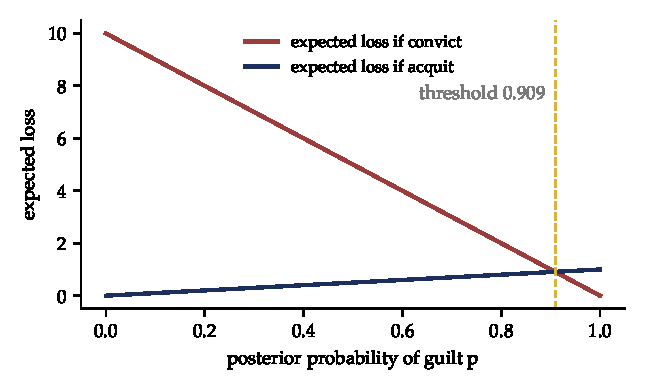
\includegraphics[width=\linewidth]{fig_threshold}
\caption{Expected loss of conviction and acquittal as functions of the posterior probability of guilt, when wrongful conviction is ten times as costly as wrongful acquittal. The two lines cross at the Blackstone threshold $10/11$.}
\label{fig:threshold1}
\end{figure}

\section{A short history of probability in the law}

\subsection{From Bernoulli to Poisson}

Probability and law grew up together. Jacob Bernoulli planned the fourth part of the \emph{Ars Conjectandi} as an application of the new calculus to civil, moral and economic affairs, and his discussion of how arguments combine was framed around legal examples: a man is found murdered, a suspect was seen nearby, he turned pale when questioned, and so on. Leibniz, trained as a lawyer, wrote of degrees of proof and wanted a logic of the probable to assist judges. Nicolas Bernoulli wrote a dissertation on the use of the art of conjecture in law, treating questions such as when a missing person may be presumed dead.\index{Bernoulli, Jacob}\index{Leibniz}

In 1785 Condorcet published his \emph{Essai} on the application of analysis to the probability of majority decisions. The result now called the Condorcet jury theorem says that if each of $n$ jurors independently reaches the correct verdict with probability $q > 1/2$, then the probability that a simple majority is correct tends to one as $n$ grows. If $q < 1/2$ it tends to zero. The theorem is a statement about the binomial distribution: with $n = 2m+1$ jurors, the probability that the majority is right is
\begin{equation}
\Prob(\text{majority correct}) = \sum_{k=m+1}^{n} \binom{n}{k} q^{k}(1-q)^{n-k},
\label{eq:condorcet}
\end{equation}
and the law of large numbers does the rest. Laplace took up the question of how large a majority should be required to convict, and Poisson's \emph{Recherches sur la probabilit\'e des jugements} of 1837 used conviction statistics from the French assize courts to estimate jurors' reliability and the prior probability that an accused was guilty \citep{poisson1837}. The Poisson distribution is named for its appearance in that book, as an approximation to the binomial, although de Moivre had derived the same limit more than a century earlier. It is still fitting that one of the most widely used distributions in science carries the name of an author whose book was about criminal justice.\index{Condorcet jury theorem}\index{Poisson, Sim\'eon Denis}

\begin{casebox}{Poisson and the French juries}
Poisson worked with published statistics on the outcomes of trials in the cours d'assises. Before 1831 a majority of seven to five sufficed to convict, and the law of 1831 required a stronger majority, eight to four. The change in conviction rates gave him leverage to estimate two unknowns: the chance that a juror judges correctly, and the prior probability that a person sent to trial is guilty. His estimates put that prior probability above one half, which is what one would expect if prosecutors screen cases before trial.
\end{casebox}

The nineteenth century then turned against the project. John Stuart Mill called the application of the calculus of probability to testimony and verdicts the real opprobrium of mathematics, and the frequentist revolution in statistics (Venn and Boole in the nineteenth century, Fisher and Neyman in the twentieth), with its insistence that probability is a long run frequency, made it hard to speak of the probability that a particular defendant is guilty. A single crime does not repeat. For much of the twentieth century the official philosophy of statistics had no vocabulary for the question every juror is asked.

\subsection{Wigmore, Turing and Good}

The revival came from two directions. John Henry Wigmore, the great American scholar of evidence, built charts of the logical relations among items of evidence and the propositions they support \citep{wigmore1913}. His charts are graphs in the modern sense, and when Schum, Kadane and others later attached probabilities to them \citep{kadane_schum1996} they became Bayesian networks, the subject of Chapter~\ref{ch:graphs}. At Bletchley Park, Alan Turing and I. J. Good developed the weight of evidence, the logarithm of the Bayes factor, as a practical tool for breaking the Enigma cipher. Good measured it in units Turing had called bans and decibans, and showed how independent items of evidence add on the log scale \citep{good1950,good1979}. After the war Good wrote extensively on the weight of evidence in law and in medicine, and his framework is the natural language for what a forensic scientist reports.\index{Wigmore, John Henry}\index{Turing, Alan}\index{Good, I. J.}\index{weight of evidence}

\subsection{Trial by mathematics}

In 1970 Michael Finkelstein and William Fairley proposed that juries in identification cases be shown how a probability of guilt would change under Bayes' rule for a range of prior probabilities \citep{finkelstein1970}. Laurence Tribe's reply, \emph{Trial by Mathematics}, became one of the most cited articles in American legal scholarship \citep{tribe1971}. Tribe argued that numbers would dwarf soft evidence, that juries could not be asked to state a prior probability of guilt without violating the presumption of innocence, and that a system that acknowledged a quantified risk of convicting the innocent would lose legitimacy. The debate has never quite ended. In England the Court of Appeal in \emph{R v Adams} told trial judges that introducing Bayes' theorem into a jury trial plunges the jury into inappropriate and unnecessary realms of theory and complexity, and in \emph{R v T} it restricted the use of likelihood ratios in footwear evidence where there was no firm statistical base \citep{donnelly2005,fenton2016}. Chapter~\ref{ch:odds} examines these cases closely.\index{Tribe, Laurence}\index{R v Adams}\index{R v T}

The academic response, led by Lindley, Fienberg, Kadane, Dawid, Aitken and Taroni, was to separate two questions that Tribe ran together. Whether a jury should be shown a formula is a question about communication and institutional design. Whether the jury's reasoning ought to obey the rules of probability is a question about rationality. A jury that convicts on evidence that should leave it in doubt is making an error whether or not anyone writes down a number. The value of the Bayesian framework is that it lets us find such errors, explain them, and design procedures that reduce them \citep{fienberg_kadane1983,aitken_taroni2004,dawid2002}.

\section{Lindley's challenge}

Lindley's 1991 paper in the \emph{Journal of the Royal Statistical Society}, \emph{Subjective Probability, Decision Analysis and Their Legal Consequences}, worked through what a court would look like if it took probability and expected utility seriously \citep{lindley1991}. Probability at the start of the trial represents what the fact finder knows before hearing evidence; probability at the end represents what is known after; and the verdict, or the sentence, should be the act that maximises expected utility given the final probability. Lindley showed that a court acting this way might impose some sanction even when the probability of guilt fell below the conventional threshold, because a graduated response can dominate the all or nothing choice between conviction and acquittal. He also offered a new solution to the gatecrasher problem, a puzzle about naked statistical evidence that we take up in Chapter~\ref{ch:standards}.

Lindley went further in conversation and in his later writing. If the task of a court is to combine probabilities with utilities in a coherent way, then that task is a computation, and computations are what machines do well. People would still be needed, he argued, to state the utilities, which express a society's values and cannot be delegated, and to supply the evidence. But the step from evidence and utilities to a verdict could in principle be made by a machine, and made more consistently than by twelve tired jurors or a single overworked judge. His view, as we understand it, was not that machines should replace judges tomorrow, but that the law should be decided by whoever, or whatever, reasons coherently, and that a properly built machine would be held to that standard more easily than a person.\index{Lindley's challenge}\index{artificial intelligence}

We call this Lindley's challenge. It was a provocation in 1991. It is a policy question in 2026, when large language models draft submissions, risk assessment tools inform bail and sentencing in many American states, and some courts experiment with automated triage of their dockets. Chapter~\ref{ch:lindleyai} returns to the challenge after we have built the tools to answer it. Our answer will be that Lindley was right about the structure and that the difficulty lies, as he said, in the utilities and in the evidence. A machine that maximises the wrong expected utility, or that learns its probabilities from biased data, is worse than a careful judge. A machine that is transparent about its probabilities and utilities, and whose computations can be verified, could be better.

\section{Objections and replies}

We state the main objections to Bayesian legal reasoning now, because they recur.

\paragraph{The presumption of innocence forbids a prior} The objection is that asking a fact finder for a prior probability of guilt presupposes that guilt is already somewhat probable, contrary to the presumption of innocence. The reply is that the presumption is a rule about burden and about the evidence that may be used, not a claim that the prior probability is zero. A prior of zero could never be moved by any evidence, so a literal reading would make conviction impossible. A natural Bayesian reading, which we develop in Chapter~\ref{ch:standards}, is that before evidence specific to the defendant is heard, he should be treated as no more likely to be guilty than any other member of the population who could have committed the crime. This gives a prior of the order of $1/N$ where $N$ is the size of that population, and it is the prior used by the defence in \emph{R v Adams}.\index{presumption of innocence}

\paragraph{Probabilities in law are not frequencies} The objection is that a probability of guilt for a single event is meaningless. The reply is that Bayesian probability is a degree of belief, made coherent by the three rules, and that the law already asks fact finders for degrees of belief when it speaks of the balance of probabilities or of proof beyond reasonable doubt. Frequencies enter as evidence about probabilities, through likelihoods and through exchangeability, but they do not exhaust them \citep{definetti1974,lindley2000}.

\paragraph{Numbers overwhelm soft evidence} Tribe's worry was that a precise statistical match probability would crowd out vague but important evidence such as an alibi. The reply is that this is a reason to quantify the soft evidence too, not to ignore the hard evidence. The Bayesian framework is a framework that tells us exactly how an alibi with a modest likelihood ratio should be weighed against a DNA match with an enormous one. In \emph{Adams} the defence did precisely that, and the arithmetic showed that the posterior probability of guilt was far lower than the raw match probability suggested (Figure~\ref{fig:adams1}).

\begin{figure}[t]
\centering
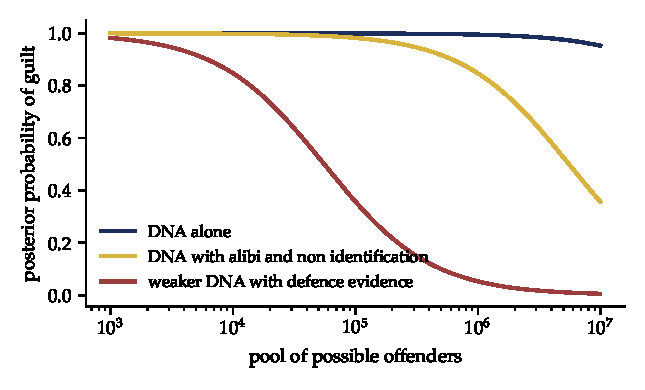
\includegraphics[width=\linewidth]{fig_adams}
\caption{Posterior probability of guilt as a function of the size of the pool of possible offenders, combining a DNA likelihood ratio with defence evidence of the kind presented in \emph{R v Adams}. The defence evidence, with a combined likelihood ratio of about one in thirty six, moves the posterior a long way when the pool is large.}
\label{fig:adams1}
\end{figure}

\paragraph{The law values reasons, not calculations} Courts give reasons, and a verdict that rests on a number may seem to lack them. The reply is that a likelihood ratio is a reason: it says how much more probable the evidence is if the claimant's story is true than if the defendant's is. The Bayesian framework disciplines reasons rather than replacing them. Chapter~\ref{ch:stories} shows how stories, the natural vehicle for legal reasons, can themselves be weighed by their likelihood ratios.

\paragraph{Juries cannot do the arithmetic} This is often true, and it is an argument for better presentation, for the use of verbal scales anchored to likelihood ratios, for graphical aids and for expert guidance, not an argument that the arithmetic is wrong. Fienberg and Kadane gave an early and careful treatment of how Bayesian analyses can be presented in legal proceedings \citep{fienberg_kadane1983}, and the forensic science community has since developed standards for reporting likelihood ratios \citep{aitken_taroni2004}.

\section{The economics of courts}

The Bayesian framework does not stop at the verdict. Courts are institutions with costs. Every hour a judge spends on one case is an hour not spent on another, and every adjournment imposes waiting costs on parties and witnesses. Gary Becker's economic approach to crime treats the probability and severity of punishment as policy instruments chosen to minimise the social cost of crime plus enforcement \citep{becker1968}. The law and economics movement, from Coase and Calabresi to Posner and Shavell, analyses rules of liability by their effects on incentives \citep{coase1960,calabresi1970,shavell1987,posner2014}. Learned Hand's formula in \emph{United States v Carroll Towing}, 159 F.2d 169 (2d Cir.\ 1947), that a party is negligent if the burden of precaution is less than the probability of harm times the gravity of the loss, is an expected cost calculation stated by a judge \citep{posner2014}. We develop these connections in Chapters~\ref{ch:tort} and~\ref{ch:becker}.

Bayesian decision theory supplies the common language. A rule of liability is a decision rule. A standard of proof is a threshold on a posterior probability. A procedural rule, such as a limit on discovery or a rule excluding evidence, is a choice about which information to collect, and its value can be measured by the expected value of sample information. Settlement is bargaining between parties with different posteriors, and the selection of disputes for trial depends on how those posteriors diverge \citep{priest_klein1984}. Even the design of a legal system, common law or civil law, adversarial or inquisitorial, can be read as a choice about how to aggregate information and how to allocate the costs of error.

\section{Machines in the courtroom}

Three technical developments make this book timely.

First, generative and deep learning methods can now approximate posterior distributions for models too complex for classical calculation. In our own work on generative Bayesian computation we train neural networks to map data directly to posterior quantiles, using simulations from the model as training data \citep{polson_sokolov_gbc}. Chapter~\ref{ch:pleadings} applies this approach to Gordon's formal model of civil pleading \citep{gordon1995}, and describes how a network trained on simulated pleadings could estimate the probability that an issue will be decided for the claimant.

Second, large language models can read and summarise legal texts at a scale no human team can match. They can also hallucinate authorities, misstate holdings and express confidence they have not earned. A Bayesian view of these systems asks whether their stated probabilities are calibrated, whether they update correctly on evidence, and whether their errors can be detected.

Third, interactive theorem provers such as Lean have changed what it means to check a proof. Mathematicians now formalise research level arguments so that every step is verified by a small trusted kernel. Lawyers and computer scientists have begun to encode statutes, notably US tax rules on the sale of a principal residence and French family benefits in the Catala language \citep{merigoux2021}, so that the computation of an entitlement can be checked against the text of the law. Chapter~\ref{ch:lean} asks how far this can go. Our view is that verification can certify the logical steps of a legal argument and the arithmetic of a Bayes factor, while leaving the probabilities and utilities, which are matters of judgment, open to argument in the ordinary way.

\section{Comparative perspectives}

The common law and the civil law reason about facts differently. In the English trial the parties control the evidence, the judge is an umpire, and the fact finder must reach a verdict on what the parties choose to present. In the French system the judge directs the inquiry, written evidence dominates, and the criminal court decides according to its \emph{intime conviction}, its inner conviction, a standard that the Code de proc\'edure p\'enale states without numbers. In Chapter~\ref{ch:commoncivil} we model these systems as different strategies for acquiring and aggregating information. The adversarial system is a pair of biased samplers whose biases are supposed to cancel; the inquisitorial system is a single sampler whose bias must be controlled by professional training and appellate review.

These differences have consequences beyond the courtroom. La Porta, Lopez de Silanes, Shleifer and Vishny argued that countries whose legal systems descend from English common law protect investors more strongly than those descended from French civil law, and that this shows up in the size of capital markets and the concentration of ownership \citep{llsv1997,llsv1998}. Their claim has been challenged and refined, but it put legal origin at the centre of development economics. In Africa, colonial history assigned common law to Ghana, Nigeria, Kenya and others, civil law to Senegal, C\^ote d'Ivoire and much of the Sahel, and both to Cameroon. Chapter~\ref{ch:africa} treats this history as a natural experiment and sets out a hierarchical Bayesian model for asking how much of the colonial legacy can be attributed to legal origin. Chapter~\ref{ch:india} turns to India, whose common law courts carry the largest backlog in the world.

\section{Order without the state}

Courts are one way to sustain cooperation. Reputations, kinship and private protection are others. Roger Gould's study of vendettas in nineteenth century Corsica, based on court records, found that revenge was rarer than the folklore suggests and that it was calibrated: it occurred mainly when the original attack involved collaboration or violence against nondisputants, and it was aimed at those who had displayed solidarity with the attacker \citep{gould2000}. Diego Gambetta's study of the Sicilian mafia treats it as an industry selling protection in a market where the state's guarantee of property was weak \citep{gambetta1993}. Both analyses are about signals and inference. A family that avenges a killing signals cohesion; a mafia boss whose threats are credible is one whose type has been revealed. Chapter~\ref{ch:gould} develops these ideas and connects them with Gould's broader argument that conflict is most likely where social rank is ambiguous \citep{gould2003}.

\section{How to read this book}

The book is in seven parts. Part I sets up the tools: decisions, probability and odds, classic cases, Bayes factors, the fallacies, the decision theoretic account of standards of proof, and the kinds of evidence. Part II applies them to English law: tort, mass torts and damages, misrepresentation, contract, family law, the Greensill affair and bankruptcy. Part III treats stories, graphical models and pleadings. Part IV, Statisticians in the Courtroom, covers Fienberg and Kadane and then applied chapters on discrimination, securities, medical evidence, intellectual property and digital evidence. Part V is comparative: common law and civil law, legal origins, Africa, India and arbitration. Part VI is about order without the state. Part VII covers costs and deterrence, antitrust, the costs of the legal system, litigation funding, sentencing and regulation, then verification, the question of artificial intelligence, explainable AI, Hume, a program for reform and the future.

Readers who want the mathematics can find a compact toolkit in Appendix~\ref{app:toolkit}, code for the main calculations in Appendix~\ref{app:code}, and a table of the principal cases in Appendix~\ref{app:cases}. Further appendices give solutions to the exercises, a glossary, a semester teaching plan and a sample examination. Each substantive chapter ends with Notes and Questions, and Appendix~\ref{app:solutions} gives solutions. Some are routine calculations; others are open questions on which we would welcome argument.

\section*{Notes and Questions}
\addcontentsline{toc}{section}{Notes and Questions}
\begin{enumerate}[label=\arabic*.]
\item Using \eqref{eq:threshold}, find the ratio of losses implied by a threshold of $0.95$, and by the civil threshold of $0.5$. What does the second imply about the relative costs of errors for claimants and defendants?
\item Compute the probability that at least seven of twelve jurors are correct, adapting \eqref{eq:condorcet} to $n = 12$, when each is right with probability $0.6$ and votes independently. Repeat for a unanimity rule, taking the probability that all twelve are correct. Why does the Condorcet theorem not apply when jurors deliberate?
\item A suspect is identified by a feature shared by one person in a thousand. The crime was committed in a city of one million adults. With a uniform prior over the city, what is the posterior probability that the suspect is the offender? What additional evidence would raise it above $0.95$?
\item State, in your own words, the difference between the probability of the evidence given innocence and the probability of innocence given the evidence. Construct a short example in which the first is one in a million and the second exceeds one half.
\item Read Tribe's \emph{Trial by Mathematics}. Which of his objections are about rationality and which about institutional design? Which do you find persuasive?
\item Lindley argued that a graduated sanction can dominate the binary choice between conviction and acquittal. Construct a three action example, convict, acquit and an intermediate order, with losses chosen so that the intermediate order is optimal for a range of posterior probabilities.
\end{enumerate}

\section*{Further reading}
Lindley's \emph{Understanding Uncertainty} is the clearest introduction to the Bayesian view \citep{lindley2006}. Aitken and Taroni give the standard treatment of forensic evidence \citep{aitken_taroni2004}. Fienberg's edited report remains the best guide to statistics in American courts \citep{fienberg1989}. Fenton, Neil and colleagues survey Bayes and the law \citep{fenton2016}. On the history, Hacking's \emph{The Emergence of Probability} and Daston's \emph{Classical Probability in the Enlightenment} are indispensable \citep{hacking1975,daston1988}.

\chapter{Bayesian Decisions for Lawyers}
\label{ch:decisions}

\section{Four questions}

Any legal decision, from a magistrate's bail order to a Supreme Court judgment, can be analysed by asking four questions. What are the possible actions? What are the possible states of the world? What is the consequence of each action in each state, and how good or bad is it? And how probable is each state, given the evidence? Bayesian decision theory answers the last question with Bayes' rule and combines the answers to all four with a single principle: choose the action with the smallest expected loss\index{expected loss}. This chapter sets out the method step by step, connects it to the language of Type I and Type II errors that lawyers meet in statistics and forensic science, and works through examples. Later chapters assume it.\index{decision theory}

\section{Objectives}

A decision needs an objective. In law, objectives are set by legislation, by precedent and by the purposes courts attribute to rules. The criminal law aims to punish and deter the guilty while protecting the innocent. Tort aims to compensate victims and to give actors incentives to take care. Contract aims to give effect to agreements and to make promises reliable. Procedure aims to resolve disputes accurately, quickly and at reasonable cost. Each objective implies a way of ranking outcomes, and the ranking is what decision theory calls a utility or, with the sign reversed, a loss.\index{objectives}

Two features of legal objectives matter for what follows. First, they are plural: a court wants accuracy, speed, low cost, fairness and legitimacy, and these conflict. A decision rule must trade them off, and the trade off should be stated. Second, they belong to society, not to the analyst. Decision theory does not tell a legislature how much worse a false conviction is than a false acquittal. It tells the legislature what its rules imply about that ratio, and what rules would implement any ratio it chooses.

\section{Actions, states and losses}

Let $\mathcal{A}$ be the set of actions open to the decision maker and $\Theta$ the set of states of the world. A loss function\index{loss function} $L(a,\theta)$ gives the loss from action $a$ when the state is $\theta$. For a criminal trial the simplest version has two actions, convict and acquit, two states, guilty and innocent, and a two by two table of losses (Table~\ref{tab:loss}). Correct decisions have zero loss; the two errors have losses $c_I$ and $c_{II}$. In the notation of Chapter~\ref{ch:why}, with $c$ for convict, $a$ for acquit, $G$ for guilt and $\bar G$ for not $G$, $c_I = L(c,\bar G)$ and $c_{II} = L(a,G)$; elsewhere in this chapter $a$ is a generic action.

\begin{table}[ht]
\centering\small
\begin{tabular}{lcc}
\toprule
& Innocent & Guilty\\
\midrule
Acquit & $0$ & $c_{II}$ (false acquittal)\\
Convict & $c_{I}$ (false conviction) & $0$\\
\bottomrule
\end{tabular}
\caption{The loss table for a criminal verdict.}
\label{tab:loss}
\end{table}

The loss table is the place where values enter. It is not a technicality. Whoever sets the criminal standard of proof, a constitutional court, the common law or a legislature, is choosing $c_I/c_{II}$, whether it says so or not.

\section{Type I and Type II errors}

\subsection{The classical vocabulary}

Classical hypothesis testing distinguishes two errors. A Type I error rejects a true null hypothesis; a Type II error fails to reject a false one. In criminal law the null hypothesis is innocence. A Type I error is convicting an innocent person; a Type II error is acquitting a guilty one. The Type I error rate, $\alpha$, is the probability of convicting given innocence; the power, $1-\beta$, is the probability of convicting given guilt, so $\beta$ is the Type II error rate.\index{Type I error}\index{Type II error}

\subsection{The trade off}

For given evidence, the two error rates trade off. A stricter standard of proof reduces $\alpha$ and raises $\beta$; a laxer one does the reverse. The receiver operating characteristic, or ROC curve, plots power against $\alpha$ as the threshold varies (Figure~\ref{fig:roc}). Better evidence moves the whole curve up and to the left, reducing both errors at once. Choosing a threshold is choosing a point on the curve; improving procedure, by better forensic science, better investigation or better presentation, is moving the curve.\index{ROC curve}

\begin{figure}[t]
\centering
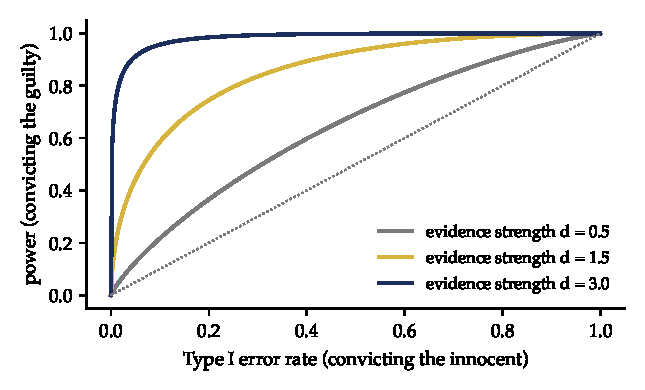
\includegraphics[width=\linewidth]{fig_roc}
\caption{ROC curves for evidence of three strengths. The standard of proof selects a point on a curve; better evidence moves the curve toward the top left corner, where both errors are small.}
\label{fig:roc}
\end{figure}

\subsection{From error rates to expected loss}

The classical approach fixes $\alpha$, conventionally at five per cent, and maximises power. The Bayesian approach minimises expected loss. If the prior probability of guilt in the cases that come to trial is $\pi$, the expected loss of a decision rule with error rates $\alpha$ and $\beta$ is
\begin{equation}
R = (1-\pi)\,\alpha\, c_I + \pi\,\beta\, c_{II}.
\label{eq:bayesrisk}
\end{equation}
Minimising $R$ over the rules on the ROC curve gives the point where the slope of the curve equals $(1-\pi)c_I/(\pi c_{II})$. The optimal $\alpha$ is not fixed at five per cent; it depends on the base rate and on the ratio of losses. In a population of defendants most of whom are guilty, a given threshold produces few false convictions in total; in a population most of whom are innocent, the same threshold produces many. This is why the Bayesian approach, which conditions on the evidence in each case, suits courts: it compares the posterior with a threshold set by the losses, and the base rate enters through the prior.\index{Bayes risk}

\subsection{Case by case: the posterior rule}

For an individual case, minimising expected loss gives the rule \eqref{eq:threshold} of Chapter~\ref{ch:why}, with $c_I = L(c,\bar G)$ and $c_{II} = L(a,G)$: convict if and only if
\begin{equation}
\Prob(\text{guilty}\given E) > \frac{c_I}{c_I + c_{II}} .
\end{equation}
This rule, applied case by case, also minimises the aggregate risk \eqref{eq:bayesrisk} across cases, provided the posteriors are computed with the same base rate and are calibrated. The two perspectives, the system's error rates and the individual posterior, are consistent: the posterior rule is the best way to run the system.

\begin{keybox}
Error rates and posteriors. A forensic test has a false positive rate of one per cent, used here as its Type I error rate, and power of ninety per cent. Of defendants tested, twenty per cent are guilty. Among positive results, the proportion from guilty defendants is $0.2\times 0.9/(0.2\times 0.9 + 0.8\times 0.01) = 0.957$. The test's error rate is one per cent, but about one positive in twenty three comes from an innocent person. If only two per cent of those tested were guilty, the proportion would fall to about $0.65$, and more than a third of positives would be innocent.
\end{keybox}

\section{Beyond two actions}

Real decisions have more than two actions. A sentencing judge chooses among discharge, fine, community order and custody of various lengths. A civil court chooses damages along a continuum. A regulator chooses among warning, fine and prosecution. Decision theory handles these by extending the loss table to each action and state, and by computing the expected loss of each action under the posterior.

\subsection{Continuous decisions and damages}

When the action is a number, such as an award of damages, and the state is the true loss $\theta$, a natural loss function is the squared error $(a-\theta)^2$ or the absolute error $|a-\theta|$. Under squared error the optimal award is the posterior mean of $\theta$; under absolute error it is the posterior median. If under compensation is worse than over compensation, an asymmetric absolute error loss leads to an award above the median, at a posterior quantile determined by the ratio of the losses. Chapter~\ref{ch:damages} develops this for the assessment of damages.\index{damages!as decision}

\subsection{Sequential decisions}

Some decisions come in sequences: whether to investigate, whether to charge, whether to accept a plea, whether to appeal. Each decision changes the information available for the next. Dynamic programming solves such problems backwards: the value of an early decision is the expected value of acting optimally afterwards. The value of information calculation of Chapter~\ref{ch:standards} is the simplest case: whether to gather more evidence before deciding.

\section{Costs of deciding}

Decisions have costs as well as consequences. A trial consumes judicial time, lawyers' fees, witnesses' time and the parties' attention. A complete objective adds the cost of the process to the expected loss of errors:
\begin{equation}
\text{total cost} = \text{cost of process} + \E[\text{loss from errors}].
\end{equation}
Spending more on a case usually reduces the expected loss from errors, by producing more and better evidence, but at a rising cost. The optimal investment equates the marginal cost of process with the marginal reduction in expected error cost. Louis Kaplow analysed this trade off in a classic article on the value of accuracy in adjudication \citep{kaplow1994}. Chapter~\ref{ch:systemcosts} applies it to the allocation of judges' time across a court system.\index{accuracy, value of}

\section{Objectives revisited: deterrence and incentives}

The losses in Table~\ref{tab:loss} describe the harm from errors in a single case. But legal decisions also shape behaviour. A rule that convicts too readily deters some innocent conduct; a rule that acquits too readily fails to deter crime. False convictions reduce deterrence, as Chapter~\ref{ch:becker} will show, because they impose sanctions whether or not one offends. The ex post loss from an error, what it costs the people in this case, and the ex ante effect of the rule on everyone's behaviour, can point in different directions. A full analysis includes both. In tort, for example, the ex post objective is to compensate the claimant accurately; the ex ante objective is to give defendants the right incentives to take care. Proportional liability for lost chances, taken up in Chapter~\ref{ch:tort}, is attractive partly because it serves both.

\section{A worked example: bail}

A magistrate must decide whether to release a defendant before trial. The actions are release and detain. The states are whether the defendant would, if released, fail to appear or commit an offence. Let the probability of such failure, given the risk assessment and the facts, be $r$. The loss from releasing a defendant who then fails is $H$, the harm to victims and the cost of recapture. The loss from detaining a defendant who would not have failed is $D$, the cost of detention to the defendant, the defendant's family and the state, which is proportional to the expected time to trial (taken here as twelve months). Release is optimal if $rH < (1-r)D$, that is if
\begin{equation}
r < \frac{D}{H + D}.
\end{equation}
If detention for the expected period costs one third as much as a failure, the threshold is one quarter: release anyone whose risk is below twenty five per cent. If delay doubles the cost of detention, the threshold rises to forty per cent. The analysis shows why delay in trials, the subject of Chapter~\ref{ch:india}, should change bail practice, and why risk assessment tools must be calibrated: the decision turns on the probability $r$, and a tool that overstates it detains people who should be released.

\section{A worked example: whether to sue}

A claimant must decide whether to bring a claim. The probability of winning is $p$, the damages if successful are $J$, the cost of litigating is $C$, and, under the English costs rule, the loser pays the winner's costs, so the claimant who loses pays the defendant's costs $C_D$ as well. A winner does not recover everything it spent: costs assessed on the standard basis usually fall well short of actual spend. Let $f$ be the fraction recovered, so that the claimant who wins recovers $fC$ and the claimant who loses pays $fC_D$. The expected value of suing under the English rule is
\begin{equation}
p\,J - C - (1-p)\,f\,C_D + p\,f\,C.
\end{equation}
The costs rules differ across systems, so it is worth comparing the common ones with the same $p$ and the same stakes. Take a claimant with a forty per cent chance of winning a hundred thousand pounds, with costs of thirty thousand on each side ($C = C_D = 30{,}000$). The recovery fraction is an assumption, not a fact about any case: we take $f = 2/3$, the figure commonly put as the typical recovery on a standard basis assessment, and apply it to both sides.

\begin{enumerate}[label=(\alph*)]
\item American rule: each side bears its own costs whatever the outcome. The claimant nets $70{,}000$ on winning and loses $30{,}000$ on losing, and the expected value is $40{,}000 - 30{,}000 = 10{,}000$.
\item English rule: costs follow the event (CPR 44.2(2)(a)). The claimant nets $100{,}000 - 30{,}000 + 20{,}000 = 90{,}000$ on winning and loses $30{,}000 + 20{,}000 = 50{,}000$ on losing. The expected value is $40{,}000 - 30{,}000 - 12{,}000 + 8{,}000 = 6{,}000$.
\item Qualified one-way costs shifting, which applies to English personal injury claims since April 2013 (CPR 44.13 to 44.17): a losing claimant ordinarily does not pay the defendant's costs, while a winning claimant still recovers part of its own. The claimant nets $90{,}000$ on winning and loses $30{,}000$ on losing, and the expected value is $40{,}000 - 30{,}000 + 8{,}000 = 18{,}000$.
\end{enumerate}

The claimant should sue if the expected value exceeds zero, adjusted for risk aversion. All three are positive here, but the rules differ in how much risk they impose. The spread between the winning and losing outcomes is $100{,}000$ under the American rule, $140{,}000$ under the English rule and $120{,}000$ under one-way shifting. The English rule gives the lowest expected value and the widest spread, so a risk averse claimant is the most likely to decline to sue, or to accept a settlement below the expected value, under it. A pre-action settlement offer, a topic Chapter~\ref{ch:becker} takes up, offers a certain amount instead. The break-even probability of winning is $0.30$ under the American rule, $5/14 \approx 0.36$ under the English rule and $0.25$ under one-way shifting, so the last encourages weak claims most. The English figures depend on the assumed recovery fraction: if $f = 1$ the English rule has expected value $40{,}000 - 30{,}000 - 18{,}000 + 12{,}000 = 4{,}000$. Litigation funding, the subject of Chapter~\ref{ch:funding}, changes this calculation by transferring risk.

\section{Summary}

Bayesian decision theory asks four questions and gives one answer. The questions are about actions, states, losses and probabilities. The answer is to minimise expected loss. Type I and Type II errors are the two ways of being wrong in a binary decision; their rates trade off along an ROC curve, and the standard of proof chooses a point on it according to the ratio of losses. Better evidence moves the curve. Costs of process, incentives and sequences of decisions extend the framework without changing its logic. The rest of the book applies it.

\section*{Notes and Questions}
\addcontentsline{toc}{section}{Notes and Questions}
\begin{enumerate}[label=\arabic*.]
\item Write down a loss table for a civil claim with actions judgment for claimant and judgment for defendant. What ratio of losses does the balance of probabilities imply?
\item For an ROC curve in which the evidence is a score that is normal with mean $0$ for the innocent and mean $d = 1.5$ for the guilty, both with standard deviation one, find the threshold that minimises expected loss when $\pi = 0.6$ and $c_I/c_{II} = 10$. What are $\alpha$ and $\beta$ at that threshold?
\item In the keybox example, find the base rate of guilt at which half of positive tests come from innocent people.
\item Under absolute error loss the optimal award is the posterior median. If under compensation is twice as bad as over compensation, at what posterior quantile should damages be set?
\item In the bail example, how should the threshold change if the expected time to trial falls from twelve months to three?
\item Recompute the English and one-way shifting expected values in the whether-to-sue example with $f = 1/2$. Which rule encourages weak claims?
\end{enumerate}

\section*{Further reading}
Lindley's \emph{Making Decisions} \citep{lindley1985}; Smith's \emph{Bayesian Decision Analysis} \citep{smith2010}; Kaplow on the value of accuracy \citep{kaplow1994}.

\chapter{Odds, Likelihood and the Weight of Evidence}
\label{ch:odds}

\section{The likelihood ratio as the currency of evidence}

The odds form of Bayes' rule, equation \eqref{eq:oddsform}, says that evidence acts on beliefs by multiplication. Whatever the prior odds of a proposition, evidence $E$ multiplies them by
\begin{equation}
\LR(E) = \frac{\Prob(E \given \Hp)}{\Prob(E \given \Hd)},
\end{equation}
where $\Hp$ and $\Hd$ are the propositions advanced by the prosecution and the defence, or by claimant and defendant. Three features of this formula explain why forensic scientists have adopted the likelihood ratio as the proper measure of the value of evidence \citep{aitken_taroni2004,evett1998}.\index{likelihood ratio}

First, the likelihood ratio is comparative. It does not ask how probable the evidence is in some absolute sense, but how much more probable it is under one account than under the other. Evidence that is equally probable under both accounts, however striking, has a likelihood ratio of one and should not move the fact finder at all. A defendant's nervousness under police questioning is common among the guilty and among the innocent who fear being disbelieved; its likelihood ratio may be close to one even though it feels incriminating.

Second, the likelihood ratio separates the role of the expert from the role of the fact finder. A DNA analyst can say how probable the observed profile is if the defendant left the stain and how probable it is if an unknown person did. The analyst cannot, without trespassing on the jury's function, say how probable it is that the defendant left the stain, because that depends on all the other evidence. The likelihood ratio is exactly the part the expert can speak to.

Third, likelihood ratios for independent items of evidence multiply, so their logarithms add. If $E_1$ and $E_2$ are conditionally independent given each hypothesis, then
\begin{gather}
\LR(E_1, E_2) = \LR(E_1)\,\LR(E_2),\\
\log \LR(E_1,E_2) = \log\LR(E_1) + \log \LR(E_2).
\end{gather}
Good, following Turing, called $10\log_{10}\LR$ the weight of evidence in decibans \citep{good1950,good1979}. A deciban is roughly the smallest change in belief a person can perceive. Ten decibans is a factor of ten, twenty is a factor of a hundred (Figure~\ref{fig:scale}). The additive scale makes it natural to think of a trial as a ledger in which each item of evidence adds or subtracts weight.\index{deciban}\index{weight of evidence}

\begin{figure}[ht]
\centering
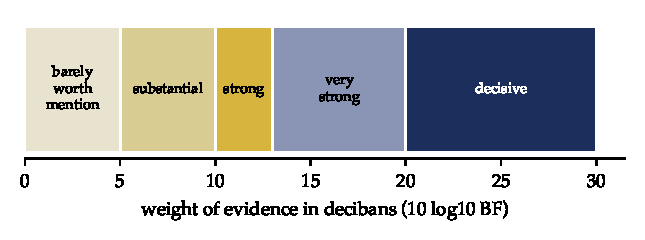
\includegraphics[width=\linewidth]{fig_scale}
\caption{A verbal scale for the weight of evidence, in decibans, in the tradition of Jeffreys and Good. The phrases used in forensic reporting differ in detail.}
\label{fig:scale}
\end{figure}

\section{The fallacies}

Most of the famous statistical errors in criminal trials are failures to distinguish $\Prob(E\given \Hd)$ from $\Prob(\Hd\given E)$, or failures to use the right $\Hd$.

\subsection{The prosecutor's fallacy}

The prosecutor's fallacy, a name due to Thompson and Schumann, is the transposition of the conditional \citep{thompson1987}. An expert testifies that the probability of a random person matching the crime stain is one in a million. Counsel, the judge or the jury then treats this as the probability that the defendant is innocent. The two are entirely different. In a city of ten million, about ten people would match. If there is no other evidence pointing to the defendant, the probability that he is the source is about one in ten, not one in a million.\index{prosecutor's fallacy}

Formally, let $N$ be the number of people who could have left the stain, let the defendant be one of them, and suppose the prior is uniform over the $N$. If the random match probability is $\gamma$ and the defendant matches, then
\begin{equation}
\Prob(\text{defendant is source} \given \text{match}) = \frac{1}{1 + (N-1)\gamma}.
\label{eq:island}
\end{equation}
This is sometimes called the island problem, because it is cleanest to imagine a crime on an island of $N$ inhabitants \citep{balding2005}. Figure~\ref{fig:population} plots \eqref{eq:island} for several match probabilities. When $N\gamma$ is small the match is close to conclusive; when $N\gamma$ is of order one or larger it is not.

\begin{figure}[t]
\centering
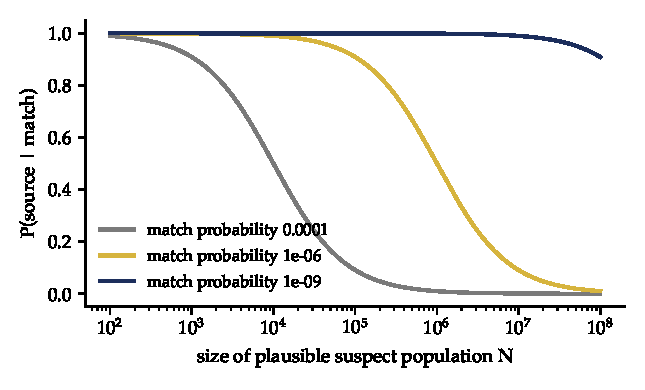
\includegraphics[width=\linewidth]{fig_population}
\caption{Probability that a person who matches a crime stain is its source, as a function of the number of possible sources, with a uniform prior and no other evidence. The prosecutor's fallacy consists in reading the match probability as the probability of innocence.}
\label{fig:population}
\end{figure}

\subsection{The defence fallacy}

The mirror image error is the defence fallacy (Thompson and Schumann's "defense attorney's fallacy"). Counsel argues that since ten people in the city match, the match shows only that the defendant is one of ten, and so it is nearly worthless. This ignores that the match has moved the defendant from being one of ten million to one of ten, a likelihood ratio of a million. Combined with substantial other evidence, such as being seen near the scene, the posterior may become high; with odds of one to ten after the match, other evidence with a likelihood ratio of about a hundred is needed to reach odds of ten to one. The match is highly relevant even though it is not conclusive by itself.\index{defence fallacy}

\subsection{The independence fallacy: People v Collins}

In 1964 a woman in Los Angeles was robbed by a young woman with a blond ponytail who fled in a yellow car driven by a black man with a beard and moustache. The prosecutor in \emph{People v Collins} called a mathematics instructor and invited him to assume probabilities for each characteristic: one in ten for a yellow car, one in four for a man with a moustache, one in ten for a girl with a ponytail, and so on. Multiplying gave one in twelve million, which the prosecutor presented as the probability that a randomly chosen couple would share all the features. The jury convicted. The Supreme Court of California reversed in 1968 \citep{collins1968}. The probabilities had no evidential foundation; the multiplication assumed independence between characteristics that are plainly correlated, such as a beard and a moustache; and even if the figure had been right, it was the probability of a random match, not the probability of innocence. The court's appendix computed, under the prosecutor's own assumptions, that the probability of at least one other matching couple in the Los Angeles area was substantial.\index{People v Collins}

\begin{casebox}{The Collins appendix}
Let $\gamma$ be the probability that a random couple has all the features and $N$ the number of couples in the area. Given that at least one couple matches, the probability that at least two match is
\[
\frac{1 - (1-\gamma)^N - N\gamma(1-\gamma)^{N-1}}{1 - (1-\gamma)^N}.
\]
With $\gamma = 1/12{,}000{,}000$ and $N = 12{,}000{,}000$, this is about $0.42$. Even on the prosecution's numbers, there was a good chance that the couple in the dock was not the only couple in the city that fitted the description.
\end{casebox}

\subsection{Sally Clark}

Sally Clark, an English solicitor, was convicted in 1999 of murdering her two infant sons, who had died suddenly in 1996 and 1998. A paediatrician testified that the chance of two sudden infant deaths in a family like hers was about one in seventy three million, obtained by squaring an estimate of one in 8{,}543 for a single death in an affluent non smoking family. The Royal Statistical Society wrote to the Lord Chancellor to point out the errors. Squaring assumed independence, ignoring genetic and environmental factors shared within a family. More fundamentally, the rarity of two cot deaths says nothing directly about guilt, because double infant murder is also extremely rare. What matters is the ratio of the two probabilities. Ray Hill's analysis of the data suggested that, conditional on two sudden deaths, the odds of natural causes against murder were between about 4.5 to 1 and 9 to 1 in favour of natural causes \citep{hill2004}. The conviction was quashed in 2003, after it emerged that the pathologist had withheld microbiological evidence that one child had a serious infection \citep{clark2003}. Sally Clark died in 2007. Her case is the clearest modern example of a prosecutor's fallacy and an independence fallacy combined, and of the human cost of statistical error.\index{Sally Clark}\index{R v Clark}

The correct comparison is between two rare events. Let $M$ denote double murder and $S$ double sudden infant death, and let $D$ be the observation that both children died suddenly with no obvious cause. Then
\[
\frac{\Prob(M \given D)}{\Prob(S\given D)} = \frac{\Prob(D\given M)}{\Prob(D \given S)} \cdot \frac{\Prob(M)}{\Prob(S)} .
\]
The first ratio may be close to one, since both explanations predict the observation. The second is the ratio of base rates, and on the available data the base rate of double sudden infant death exceeded that of double infant homicide. The figure of one in seventy three million was a poor estimate of $\Prob(S)$, and even a sound estimate of $\Prob(S)$ says nothing until it is set against $\Prob(M)$.

\section{R v Adams: Bayes in front of the jury}

Denis Adams was charged with a rape committed in 1991. The only evidence linking him to the crime was a DNA match, with a reported match probability of one in two hundred million. Everything else pointed the other way. The victim did not pick him out at an identification parade and said he did not resemble her attacker. He was older than the man she described. His girlfriend gave him an alibi. The defence called Peter Donnelly, a professor of statistics, to explain to the jury how to combine the evidence using Bayes' rule, with a questionnaire that led jurors through the calculation for their own chosen numbers \citep{donnelly2005}.\index{R v Adams}\index{Donnelly, Peter}

Adams was convicted. On appeal in 1996 the Court of Appeal ordered a retrial \citep{adams1996}, but it was hostile to the use of Bayes' theorem, saying that it trespassed on the jury's task of evaluating evidence as a whole. At the retrial the defence again led the jury through the method; Adams was again convicted; and on the second appeal in 1997 the Court of Appeal said that the method should not be used in a jury trial without special reason, while offering no alternative account of how the jury should combine the DNA evidence with the rest \citep{adams1998}.

The Adams calculation is worth doing. Suppose the pool of possible offenders is the adult male population within a plausible distance, perhaps one hundred and fifty thousand men. With a uniform prior the prior odds are about $1$ to $150{,}000$. The DNA likelihood ratio, taken at face value, is $2\times 10^8$, which raises the odds to about $1{,}300$ to $1$. The failure of the victim to identify Adams might have a likelihood ratio of around one in nine; the alibi, if given moderate weight, perhaps one in four. Together these give a factor of one in thirty six, bringing the odds to about $37$ to $1$, or a posterior probability of about $0.97$. With a larger pool, a weaker DNA likelihood ratio once laboratory error is considered, or stronger defence evidence, the posterior falls quickly below any plausible criminal threshold, as Figure~\ref{fig:adams1} shows. The point is not that Adams was innocent. The point is that the conclusion depends on judgments the jury was entitled to make, and that without the arithmetic it had no way to see how much those judgments mattered.

\section{R v Doheny and the guidance on DNA}

In \emph{R v Doheny and Adams}, decided in 1996 (reported in 1997; Gary Adams, a different Adams from the case above), the Court of Appeal gave guidance on presenting DNA evidence that is, on its face, Bayesian \citep{doheny1997}. The expert should explain the random match probability and may say how many people in the United Kingdom, or in a relevant subpopulation, would be expected to share the profile. The judge should direct the jury that if, say, four or five people in the country share the profile, the question is whether they are satisfied, in the light of all the evidence, that the defendant is the one who left the stain. This is the island problem expressed in words. The court accepted the logic of the likelihood ratio while rejecting the formula.\index{R v Doheny}

\section{R v T and the limits of likelihood ratios}

In \emph{R v T}, a 2010 murder appeal, the issue was footwear marks. The prosecution's expert had used a likelihood ratio approach, drawing on a database of shoe distribution data to estimate how common the pattern was, and had expressed his conclusion on a verbal scale corresponding to a likelihood ratio at the top of the moderate band (about a hundred). The Court of Appeal held that the likelihood ratio should not be used for footwear evidence where there was no reliable statistical basis for the underlying frequencies, and that the expert's report had not been transparent about how the conclusion was reached \citep{rvt2010}. Forensic statisticians responded that the court had misunderstood the role of the likelihood ratio, which is a framework for reasoning rather than a claim about the precision of the inputs, and that any expert opinion on the significance of a match implicitly makes the same comparison \citep{berger2011}.\index{R v T}

Both sides have a point. The court was right that numbers with no foundation should not be dressed in the authority of calculation, which was the lesson of \emph{Collins}. The statisticians were right that the alternative, an unquantified opinion that a mark could have been made by the shoe, hides the same reasoning without making it better. The constructive response is to require that every likelihood ratio presented in court come with an account of its inputs and their uncertainty, and that experts report ranges where the inputs are soft. We develop this in Chapter~\ref{ch:bf}.

\section{Relevance as a likelihood ratio}

The English law of evidence defines relevance loosely. In \emph{DPP v Kilbourne} Lord Simon said that evidence is relevant if it is logically probative or disprobative of some matter requiring proof \citep{kilbourne1973}. Rule 401 of the United States Federal Rules of Evidence says that evidence is relevant if it has any tendency to make a fact more or less probable than it would be without the evidence, and the fact is of consequence in determining the action. Both definitions have a natural Bayesian reading. Evidence $E$ makes $\Hp$ more probable exactly when $\LR(E) > 1$ and less probable when $\LR(E) < 1$. Irrelevant evidence is evidence with likelihood ratio one.\index{relevance}

This reading clarifies several doctrines. Evidence of a defendant's bad character is relevant if people who commit crimes of the kind charged are more likely to have such a history than people who do not. It may nonetheless be excluded because its probative value is outweighed by prejudice, which in Bayesian terms means, in part, that the jury is likely to overweight it, treating a likelihood ratio of three as if it were three hundred. The exclusionary rule then becomes a correction for a predictable cognitive error rather than a claim that the evidence is irrelevant.

Lord Hoffmann put the general point memorably in \emph{Re B (Children)}: if a legal rule requires a fact to be proved, a judge must decide whether or not it happened, and there is no room for a finding that it might have happened \citep{reb2008}. The law operates a binary system in which the only values are zero and one. The Bayesian reading is that the fact finder forms a posterior probability, compares it to a threshold, and then treats the fact as established or not for the purposes of the legal consequence. The binary system is about the decision, not about the belief.

\section{The weight of evidence as a sequential test}

Turing's use of the weight of evidence at Bletchley was sequential. Each new intercept added weight, and the decision to act was made when the cumulative weight crossed a threshold. Wald's sequential probability ratio test, developed at the same time in the United States, has the same structure. A trial can be read the same way. Each witness, each document, each forensic report adds a weight, positive or negative, and the verdict is reached when the total crosses a threshold. Figure~\ref{fig:decibans} shows simulated paths of cumulative weight for a guilty and an innocent defendant.\index{sequential test}

\begin{figure}[t]
\centering
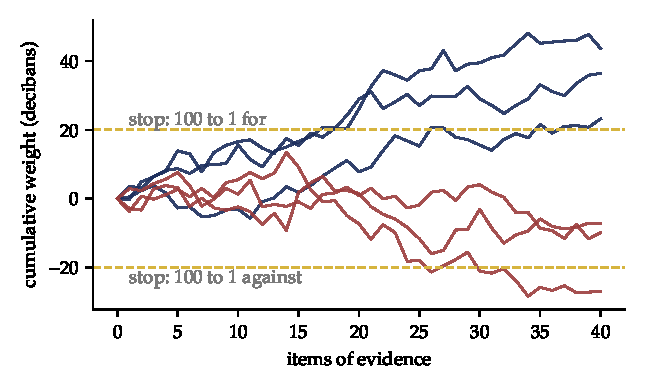
\includegraphics[width=\linewidth]{fig_decibans}
\caption{Simulated paths of cumulative weight of evidence in decibans. Paths generated under guilt drift upward (blue in the digital edition), paths generated under innocence drift downward (red). The dashed lines mark thresholds of twenty decibans, a factor of one hundred.}
\label{fig:decibans}
\end{figure}

The sequential view explains features of trial procedure. The prosecution goes first because it bears the burden; if the weight it adds does not reach a minimum, the judge may withdraw the case from the jury on a submission of no case to answer. The defence then adds its evidence, which typically has negative weight. The jury does not stop part way, because the rules require it to hear everything, but the order in which evidence is heard affects how people weigh it, and much of the craft of advocacy is about sequencing.

The additivity of weights holds only when items are conditionally independent. When they are not, as when two witnesses spoke to each other before testifying, or when a confession and the physical evidence both derive from a police theory, adding weights double counts. Graphical models, the subject of Chapter~\ref{ch:graphs}, are the tool for keeping track of dependence.

\section{Verbal scales and their dangers}

Where juries are not given numbers, as is usual for evidence other than DNA, forensic scientists in England and elsewhere often report likelihood ratios on a verbal scale: weak support, moderate support, moderately strong support, strong support, very strong support, extremely strong support, each corresponding to a range of likelihood ratios. The guidance of the European Network of Forensic Science Institutes is an example. Verbal scales have two dangers. People interpret the same phrase differently, so that strong support may be heard as almost conclusive by one juror and as fairly weak by another. And the phrases describe the evidence, not the hypothesis, but are easily heard as statements about guilt. Research on how lay people interpret such phrases shows wide variation, and some studies find that weak verbal expressions of inculpatory evidence can lower, rather than raise, belief in guilt. A reasonable compromise is to report the number and the phrase together, with an explanation that the number says how many times more probable the evidence is under one account than under the other, and with a reminder that it does not say how probable either account is.

\section{Bayes and the lay fact finder}

Experimental work on juries suggests that people are not hopeless Bayesians. They often update in the right direction, but by too little when evidence is statistical and by too much when it is vivid. Kahneman and Tversky's work on base rate neglect is directly relevant: told that a cab in a hit and run accident was identified as blue by a witness who is right eighty per cent of the time, in a city where fifteen per cent of cabs are blue, most people put the probability that the cab was blue near eighty per cent, while Bayes' rule gives about forty one per cent \citep{tversky1982}. The legal system's response to these biases is partly procedural, through rules of exclusion and judicial directions, and partly structural, through the use of professional judges, appellate review and reasons. A Bayesian analysis can inform each of these responses by identifying where the biases are likely to bite.\index{base rate neglect}

\begin{keybox}
The cab problem. Let $B$ be the event that the cab was blue and $W$ that the witness says blue. With $\Prob(B) = 0.15$, $\Prob(W\given B) = 0.8$ and $\Prob(W\given \bar B) = 0.2$,
\[
\Prob(B\given W) = \frac{0.8\times 0.15}{0.8 \times 0.15 + 0.2 \times 0.85} = \frac{0.12}{0.29} \approx 0.41.
\]
The likelihood ratio of the testimony is four, and the prior odds are about $0.18$, so the posterior odds are about $0.71$.
\end{keybox}

\section{The blue bus and naked statistics}

In \emph{Smith v Rapid Transit}, a Massachusetts case from 1945, the plaintiff was forced off the road at night by a bus she could not identify. The defendant company operated the only franchised bus line on that street. The court held that this was not enough: the probability that the bus belonged to the defendant might be high, but a verdict must rest on actual belief, not on a mathematical chance \citep{smith1945}. Philosophers have built a large literature on the hypothetical in which eighty per cent of the buses in a town are blue and belong to one company. Should a plaintiff hit by an unidentified bus recover against that company on the balance of probabilities? Many philosophers have argued that naked statistical evidence is inherently insufficient.\index{blue bus problem}\index{naked statistical evidence}

The Bayesian analysis distinguishes three issues. The first is whether the statistic is the right prior. Eighty per cent of buses is not the same as eighty per cent of buses on that road at that hour, and the plaintiff who has done no more is presenting a weak prior with no likelihood ratio at all. The second is the incentive effect. If plaintiffs could recover on market share alone, the dominant company would bear liability for its competitors' negligence, and neither firm would have the right incentive to take care. The third is the effect on investigation. A rule that rewards naked statistics discourages the collection of individual evidence, whose expected value of information may be large. Each of these is a reason, in decision theoretic terms, for refusing liability on naked statistics, and none of them requires the claim that statistical evidence is not evidence. Chapter~\ref{ch:standards} takes up the related gatecrasher problem and its solution by expected utility.

\section*{Notes and Questions}
\addcontentsline{toc}{section}{Notes and Questions}
\begin{enumerate}[label=\arabic*.]
\item Show that if $\LR(E) = 1$ then $\Prob(\Hp\given E) = \Prob(\Hp)$ for every prior. Show conversely that if the posterior equals the prior for some prior strictly between zero and one, then $\LR(E) = 1$.
\item In the island problem with $N = 10^6$ and $\gamma = 10^{-6}$, compute the posterior probability that the matching defendant is the source. Suppose a second, independent trait with frequency $1/50$ is also shared. What is the new posterior?
\item Reproduce the calculation in the Collins casebox. Then suppose the true frequency of the combination was one in a hundred thousand. How does the conclusion change?
\item In the Sally Clark case, suppose the probability of a second sudden infant death given a first is one in a hundred rather than one in 8{,}543. Recompute the probability of two deaths in such a family. What does this imply about the independence assumption?
\item Write down a defence argument in the style of \emph{Adams} for a case with a DNA likelihood ratio of $10^7$, a pool of $500{,}000$, a failed identification with likelihood ratio $1/5$, and an alibi with likelihood ratio $1/3$. What is the posterior probability of guilt?
\item Find an example of evidence that is relevant under Rule 401 but would plausibly be overweighted by a jury. Describe a direction that might correct the bias.
\end{enumerate}

\section*{Further reading}
Aitken and Taroni \citep{aitken_taroni2004} and Evett and Weir \citep{evett1998} are standard. Balding's book on DNA evidence is clear and careful \citep{balding2005}. Donnelly's account of \emph{Adams} \citep{donnelly2005} and Hill's analysis of cot deaths \citep{hill2004} reward close reading, and both are collected in Kadane's casebook \citep{kadane2008}.

\chapter{Classic Problems: Simpson, the Island and the Search}
\label{ch:classic}

\begin{quote}\itshape
The question is not the probability that a batterer goes on to murder his wife. The question is the probability that a batterer murdered his wife, given that she has been murdered.
\par\hfill\normalfont after I. J. Good, 1995
\end{quote}

This chapter collects three problems that every student of evidence should be able to work. The first is the argument made for the defence in the criminal trial of O. J. Simpson about the significance of prior domestic violence, which we use in our Booth course on Bayes and artificial intelligence as the cleanest example of conditioning on the wrong event. The second is the island problem, the canonical model of forensic identification, in the coherent form given by Philip Dawid and Julia Mortera. The third is the problem of search, which shows how the way a suspect was found changes the analysis. We close with the graphical tools that Dawid, Mortera and Jim Smith have developed for cases too complex to work by hand, and with their recent comparison of methods on the Kercher evidence. Later sections name the error in the Simpson argument as the Dershowitz fallacy and set out the work of Balding and Donnelly on DNA evidence. The level is that of a first year evidence class that is willing to do arithmetic.

\section{The Simpson argument}

\begin{casebox}{People v Simpson (Los Angeles Superior Court, 1995)}
On 12 June 1994 Nicole Brown Simpson and Ronald Goldman were stabbed to death outside her home in Brentwood. Her former husband, O. J. Simpson, was charged with both murders. The prosecution's case combined blood and DNA evidence, a glove found at his home, and a history of domestic violence: he had pleaded no contest to spousal battery in 1989, and there were recorded calls to the police. The defence attacked the collection and handling of the physical evidence and the credibility of a detective. On 3 October 1995 the jury acquitted. In a civil action brought by the victims' families, a jury in Santa Monica found him liable for wrongful death in 1997 and awarded damages of about thirty three million dollars. The two verdicts are consistent with a posterior probability between the civil and criminal thresholds, a point we return to below.
\end{casebox}

\subsection{Dershowitz's statistic}

Alan Dershowitz, a member of the defence team, argued in public and later in his book \emph{Reasonable Doubts} that the evidence of battering was nearly irrelevant to the question of murder \citep{dershowitz1996}. Roughly four million women are battered by their partners each year in the United States, he said, and only about fifteen hundred are murdered by them. So fewer than one battered woman in 2,500 is killed by her batterer in a given year. The prosecution's suggestion that battering is a prelude to murder was, on this view, statistically baseless.\index{Simpson, O. J.}\index{Dershowitz, Alan}

The figure may be roughly right. The inference is wrong. Let $B$ denote the event that a woman was battered by her partner, $K$ the event that she was killed by her partner, and $M$ the event that she was murdered by someone. Dershowitz computed
\[
\Prob(K \given B) \approx \frac{1}{2{,}500}.
\]
This answers the question: how likely is it that a battered woman will be killed by her partner? But Nicole Brown Simpson had been killed. The jury already knew $M$. The relevant question was
\[
\Prob(K \given B, M),
\]
the probability that a battered woman who has been murdered was murdered by her batterer.

\subsection{Good's correction}

I. J. Good wrote a short note in \emph{Nature} in 1995 making exactly this point \citep{good1995}, and Merz and Caulkins made a similar analysis with American homicide data \citep{merz1995}. The calculation is a direct application of Bayes' rule. A battered woman who is murdered was either killed by her batterer or by someone else. Over a year,
\[
\Prob(K \given B) \approx \frac{1}{2{,}500}
\]
on Dershowitz's own numbers, while the probability that a woman is murdered by someone other than her partner is roughly the general rate of homicide of women by non partners, of the order of
\[
\Prob(M\cap\bar K \given B) \approx \frac{1}{20{,}000}
\]
per year. Hence
\begin{equation}
\begin{split}
\Prob(K\given B, M) &= \frac{\Prob(K\given B)}{\Prob(K\given B) + \Prob(M \cap \bar K \given B)}\\
&\approx \frac{1/2{,}500}{1/2{,}500 + 1/20{,}000} = \frac{8}{9} \approx 0.89 .
\end{split}
\label{eq:simpson}
\end{equation}
Among battered women who are murdered, the large majority were murdered by their batterers. The history of battering, far from being irrelevant, is strong evidence once the murder is taken into account. The likelihood ratio of the battering for the proposition that the husband was the killer, comparing murdered women killed by partners with those killed by others, is large, because battering is far more common among the former.\index{Good, I. J.}

\begin{keybox}
The Simpson lesson. Conditioning on the wrong event is as dangerous as transposing the conditional. Dershowitz's figure was $\Prob(K\given B)$. The relevant figure was $\Prob(K\given B, M)$. The fact of the murder is part of the evidence, and it changes the reference class from all battered women to murdered battered women.
\end{keybox}

\subsection{Teaching the example}

In class we present Simpson in three steps. First students compute Dershowitz's figure and are asked whether it shows that the battering is irrelevant. Most say yes. Then we draw a tree: battered women, divided into those killed by their partner this year, those killed by someone else, and those not killed. The branch that matters is the union of the first two, because the woman is dead. Finally we ask students to state the likelihood ratio of the battering evidence for the hypothesis that the husband is the killer, using the base rates of partner and non partner homicide, and to see that it is of order ten or more. The tree is shown in Figure~\ref{fig:simpsontree}.

\begin{figure}[t]
\centering
\begin{tikzpicture}[grow=right, level distance=3.2cm, sibling distance=1.3cm,
  every node/.style={font=\small},
  edge from parent/.style={draw, -{Stealth[length=2mm]}, nightblue}]
\node[draw, rounded corners, fill=softgray] {Battered woman}
  child {node[draw, rounded corners] {Not murdered} edge from parent node[below, sloped, font=\scriptsize] {$\approx 0.99955$}}
  child {node[draw, rounded corners, fill=starlight!30] {Killed by other} edge from parent node[above, sloped, font=\scriptsize] {$1/20{,}000$}}
  child {node[draw, rounded corners, fill=starlight!60] {Killed by partner} edge from parent node[above, sloped, font=\scriptsize] {$1/2{,}500$}};
\end{tikzpicture}
\caption{The Simpson tree for one year. The evidence that the woman was murdered removes the bottom branch. Of the remaining probability, eight ninths lies on the branch in which the partner is the killer.}
\label{fig:simpsontree}
\end{figure}

\subsection{Two verdicts}

The criminal and civil verdicts in Simpson are often cited as contradictory. They are not. A jury that put the probability of guilt at $0.8$ should acquit under a criminal threshold of $0.9$ or more and find liability under the civil threshold of $0.5$. The civil trial also differed in its evidence: Simpson testified and was cross examined, and photographs emerged of him wearing shoes of the rare type whose prints were found at the scene, which he had denied owning. Different evidence and a different threshold can lead to different verdicts without inconsistency. Chapter~\ref{ch:standards} develops the standards of proof that the Simpson cases illustrate.

\subsection{Defence arguments about the laboratory}

The defence also argued that the blood evidence could have been contaminated or planted. In the language of Chapter~\ref{ch:odds}, the defence was attacking the denominator of the likelihood ratio. If there is a probability $c$ that an innocent defendant's blood ends up on an item through contamination or planting, the likelihood ratio of a match cannot exceed roughly $1/c$, however rare the profile. The prosecution's emphasis on vanishingly small match probabilities was beside the point if the jury believed $c$ was of order one in a hundred. A Bayesian analysis would have focused the trial on the right question: not how rare the profile was, but how likely it was that the profile could appear on the items for reasons other than the defendant's presence at the scene.

\section{The island problem}

\subsection{Statement}

A crime is committed on an island with $N+1$ inhabitants. The criminal is one of them. A trace left at the scene shows a characteristic, such as a DNA profile, that the criminal is known to have. Each inhabitant other than the criminal independently has the characteristic with probability $p$. A suspect $S$ is found, by means that are independent of the characteristic, and is found to have it. What is the probability that $S$ is the criminal?\index{island problem}

\subsection{The coherent solution}

Dawid gave a careful treatment of the problem in a volume in honour of Lindley \citep{dawid1994}, and Dawid and Mortera extended it to cover uncertainty about $p$ and different search strategies \citep{dawid1996}. Balding and Donnelly gave a parallel analysis in the same period \citep{balding1995}. With a uniform prior over the inhabitants, so that $\Prob(G) = 1/(N+1)$ where $G$ is the event that $S$ is guilty, the likelihood ratio of the match is $1/p$, and
\begin{equation}
\Prob(G\given \text{match}) = \frac{1}{1 + Np}.
\label{eq:islandsimple}
\end{equation}
This is equation~\eqref{eq:island} of Chapter~\ref{ch:odds}, except that here $N$ counts only the alternatives to $S$ (there it counted everyone, $S$ included) and the match probability is written $p$ rather than $\gamma$. Several features deserve emphasis. It depends on $N p$, the expected number of innocent people with the characteristic, and not on $p$ alone. The likelihood ratio $1/p$ is the same whether $S$ was chosen at random or identified by other evidence, provided that evidence is independent of the characteristic; but such evidence changes the prior, and then \eqref{eq:islandgeneral} below replaces \eqref{eq:islandsimple}. And it ignores the possibility that other inhabitants have been tested.

\subsection{Uncertainty about the match probability}

In practice $p$ is not known. It is estimated from a database, and different experts may disagree about the relevant population. Dawid and Mortera showed that the coherent answer replaces $p$ with a function of its distribution. Suppose $p$ has a prior distribution with mean $\mu$ and variance $\sigma^2$, and write $\E$ for expectation. The probability that an innocent inhabitant has the characteristic, given that the criminal does, is the predictive probability of a further match given one observed match, which is
\begin{equation}
\E(p\given \text{one match}) = \frac{\E(p^2)}{\E(p)} = \mu + \frac{\sigma^2}{\mu}.
\label{eq:dawidmortera}
\end{equation}
The relevant match probability is not the mean of $p$ but its size biased mean, which is always at least as large. Uncertainty about $p$ always weakens the identification evidence. Then
\begin{equation}
\Prob(G\given \text{match}) = \frac{1}{1 + N(\mu + \sigma^2/\mu)} .
\end{equation}
This is a striking and practically important result. A laboratory that reports only its best estimate of $p$ overstates the strength of a match when that estimate is uncertain. Equation \eqref{eq:dawidmortera} is also the reason the subpopulation correction, which Chapter~\ref{ch:bf} develops, raises the match probability: relatedness within a subpopulation makes allele frequencies uncertain from the point of view of the analyst.\index{Dawid, Philip}\index{Mortera, Julia}

\subsection{Search}

Now suppose $S$ was not found independently of the characteristic but by a search: inhabitants were tested in random order until one matched. Dawid and Mortera, and Balding and Donnelly, showed that the posterior probability of guilt is then larger than \eqref{eq:islandsimple}, because the search has eliminated those tested before $S$. If $k$ inhabitants were tested and excluded before $S$ matched, the effective population of alternatives falls from $N$ to $N - k$, and
\begin{equation}
\Prob(G\given \text{search}) = \frac{1}{1 + (N-k)p}.
\end{equation}
In the extreme case where all other inhabitants are tested and none match, $S$ is certainly guilty. This is the formal content of the Balding and Donnelly argument that a database search slightly strengthens the case against the person found. The intuition that searching through many people to find a match is a fishing expedition that should weaken the evidence is correct only for a different question: how probable it is that the search finds some innocent match. For the question the court must decide, whether this person is the criminal, the excluded inhabitants are evidence for guilt. Table~\ref{tab:island} gives numerical examples.\index{database search}

\begin{table}[t]
\centering\small
\begin{tabular}{lccc}
\toprule
Scenario & $N$ & effective $p$ & $\Prob(G\given\cdot)$\\
\midrule
Independent identification, $p$ known & $10^5$ & $10^{-6}$ & $0.909$\\
Same, $p$ uncertain, $\sigma = \mu$ & $10^5$ & $2\times 10^{-6}$ & $0.833$\\
Search, $50{,}000$ excluded & $10^5$ & $10^{-6}$ & $0.952$\\
Independent identification, larger island & $10^6$ & $10^{-6}$ & $0.500$\\
\bottomrule
\end{tabular}
\caption{Island problem variants. Uncertainty about the match probability weakens the evidence; search through a population that excludes others strengthens it; a larger island weakens it.}
\label{tab:island}
\end{table}

\subsection{Relatives and other complications}

The island model assumes that innocent inhabitants have the characteristic independently. For DNA this fails for relatives: a brother of the criminal has a far higher chance of sharing the profile than a stranger. If the suspect has a brother on the island who is not excluded, the posterior probability of guilt is substantially reduced, because the brother is a credible alternative. The coherent analysis sums over the population with individual match probabilities $p_i$:
\begin{equation}
\Prob(G\given \text{match}) = \frac{\pi_S}{\pi_S + \sum_{i\ne S} \pi_i\, p_i},
\label{eq:islandgeneral}
\end{equation}
where $\pi_i$ is the prior probability that inhabitant $i$ is the criminal. This general form, in which each alternative contributes its prior weight times its probability of matching, is the cleanest statement of how identification evidence should be weighed. It also shows that the law's habit of asking whether a match is unique to the defendant is the wrong question. What matters is the total weight $\sum_{i\ne S}\pi_i p_i$ of alternative explanations.

\section{Jim Smith and the structure of evidence}

Jim Smith of the University of Warwick has worked on Bayesian decision analysis for four decades, and his textbook sets out a careful methodology for eliciting probabilities and utilities from decision makers and checking their coherence \citep{smith2010}. In forensic and legal work his distinctive contribution is the chain event graph, a graphical model built from an event tree rather than from a set of variables \citep{smith2008,collazo2018}.\index{Smith, Jim Q.}\index{chain event graph}

\subsection{Why event trees}

A Bayesian network, the subject of Chapter~\ref{ch:graphs}, represents a problem as a set of variables with conditional independence relations encoded by a directed acyclic graph. It works best when every variable is defined in every scenario. Legal stories are not like that. If the defendant was at home all evening, the variable describing how he travelled to the scene is undefined. If the knife was never at the scene, the variable describing its contamination at the scene is meaningless. The prosecution and defence accounts have different shapes. Forcing them into a common set of variables introduces artificial states and obscures the structure.

An event tree describes the ways the story can unfold. Each path from the root is a possible history; each branching is a point of uncertainty, with probabilities on its edges. The prosecution's histories and the defence's histories are different subtrees, and evidence is a set of leaves. Chain event graphs compress the tree by merging nodes whose future development is probabilistically identical, so that conditional independence becomes visible as shared structure. Riccomagno and Smith showed how to represent causal manipulations on such graphs \citep{riccomagno2007}, which in legal terms means representing interventions, such as what would have happened had the defendant not acted.

\begin{figure}[t]
\centering
\begin{tikzpicture}[node distance=1.1cm and 1.9cm, every node/.style={font=\scriptsize},
 st/.style={circle, draw=nightblue, fill=softgray, minimum size=5mm, inner sep=1pt},
 sink/.style={rectangle, rounded corners, draw=nightblue, fill=starlight!35, inner sep=3pt},
 ar/.style={-{Stealth[length=1.6mm]}, nightblue}]
\node[st] (r) {$w_0$};
\node[st, above right=0.6cm and 1.8cm of r] (a) {$w_1$};
\node[st, below right=0.6cm and 1.8cm of r] (b) {$w_2$};
\node[st, right=of a] (c) {$w_3$};
\node[st, right=of b] (d) {$w_4$};
\node[sink, right=1.6cm of c] (p) {high trace found};
\node[sink, right=1.6cm of d] (q) {low trace found};
\draw[ar] (r) -- node[above, sloped] {handled drugs} (a);
\draw[ar] (r) -- node[below, sloped] {did not} (b);
\draw[ar] (a) -- node[above] {notes in pocket} (c);
\draw[ar] (b) -- node[below] {notes circulated} (d);
\draw[ar] (c) -- node[above] {high trace} (p);
\draw[ar] (c) -- node[pos=0.3, above, sloped] {low trace} (q);
\draw[ar] (d) -- node[below] {low trace} (q);
\draw[ar] (d) -- node[pos=0.3, below, sloped] {high trace} (p);
\end{tikzpicture}
\caption{A stylised chain event graph for an activity level question about drug traces on banknotes, in the spirit of Robertson, Wilson and Smith. Histories are routed to two sinks fixed by the finding. The likelihood ratio of a high trace compares the probability of reaching the high-trace sink from $w_1$ with the probability of reaching it from $w_2$.}
\label{fig:ceg}
\end{figure}

\subsection{Activity level propositions}

Forensic science distinguishes source level propositions, whose DNA is this, from activity level propositions, how did it get there. Most of the difficult questions in modern trials are at the activity level. Robertson, Wilson and Smith have applied chain event graphs to a drug trafficking case involving traces of drugs on banknotes, where the question was whether high levels of contamination indicated involvement in dealing or could be explained by general circulation \citep{robertson2024}. Their modification of the standard chain event graph introduces two sink nodes, one for each possible finding about the traces. The likelihood ratio is then the ratio of the probability of reaching the observed sink given the prosecution proposition (the suspect handled drugs), that is from $w_1$, to the probability of reaching it given the defence proposition, from $w_2$. Figure~\ref{fig:ceg} sketches the idea.\index{activity level propositions}

\section{Object oriented networks: Dawid and Mortera on DNA}

Dawid and Mortera, with Lauritzen, Pascali, van Boxel and Vicard, developed probabilistic expert systems for forensic genetics \citep{dawid2002pes,mortera2003,dawid2007oobn}. The building blocks are Bayesian networks for the inheritance of alleles at a genetic marker: nodes for the paternal and maternal genes of each person, for the genotype, and for observed typing results. These blocks are combined in object oriented networks in which a person, a marker or a mixture is a reusable class. The approach handles problems that are intractable by hand: disputed paternity with missing parents, identification of victims in mass disasters using relatives' profiles, mixtures with several contributors, and mutation.

The method illustrates a general principle. Complex evidence should be analysed by building a model from well understood components and letting the computer do the bookkeeping. The analyst's judgment goes into the structure and the parameters, which can be argued about; the arithmetic is mechanical and can be checked. This is the division of labour we will defend in Chapter~\ref{ch:lean} when we discuss formal verification.

\section{Three methods on one case: Kercher}

In 2024 Dawid, Dotto, Mortera, Graves, Kadane, Robertson, Smith and Wilson compared three graphical methods, Wigmore charts, Bayesian networks and chain event graphs, on part of the evidence in the first trial of Amanda Knox and Raffaele Sollecito for the murder of Meredith Kercher \citep{dawid2024kercher}. Their conclusion is that the methods serve different audiences. Wigmore charts suit lawyers, because they display the argumentative structure of the case, the chain from evidence to ultimate proposition, without requiring numbers. Bayesian networks suit forensic scientists, who need to compute likelihood ratios for specific items such as a DNA trace. Chain event graphs suit the police, because they show how events could have unfolded in time and which scenarios different findings would distinguish. A complete analysis of a case might use all three.

We return to the Kercher case in Chapter~\ref{ch:stories}, where it is the worked example for our theory of stories. The point here is that several of the leading Bayesian statisticians of the law, working together, reached a pluralist conclusion: there is no single correct picture of a case, but there is a single correct calculus for combining the pieces once they are drawn.

\section{The Dershowitz fallacy}

The error in the Simpson argument deserves its own name, and we call it the Dershowitz fallacy. It is a form of what Thompson and Schumann called the defense attorney's fallacy \citep{thompson1987}, and it is distinct from the prosecutor's fallacy of Chapter~\ref{ch:odds}. The prosecutor's fallacy transposes a conditional, reading $\Prob(E\given \bar G)$, with $E$ the evidence, as $\Prob(\bar G\given E)$. The Dershowitz fallacy conditions on too little: it computes a probability within a reference class that ignores part of what is known. In Simpson the omitted fact was the murder itself. The general form is
\[
\text{report } \Prob(H\given E_1) \quad\text{when the question is}\quad \Prob(H \given E_1, E_2),
\]
where $E_2$ is evidence that both sides accept and that changes the reference class. Because $E_2$ is uncontroversial, its omission is easy to miss.\index{Dershowitz fallacy}

The fallacy is persuasive because the reported number is true. Fewer than one battered woman in 2,500 is killed by her partner in a given year. A juror who checks the number will find it correct. The error lies in the question the number answers, and that error is invisible unless one asks what event the probability is conditioned on. This is why we teach students always to write down the conditioning event in full before interpreting any probability offered in court.

\subsection{Other instances}

The same structure appears in many settings.
\begin{description}
\item[{\mdseries Medical negligence}] An expert testifies that a particular complication follows a procedure in only one case in a thousand, so the surgeon's technique was probably not at fault. But the patient suffered the complication. The relevant question is the probability that a complication which has occurred was caused by poor technique, which depends on how often poor technique occurs and on the rate of complications with poor technique relative to the rate with good technique.
\item[{\mdseries Product liability}] A manufacturer shows that its product fails in only one unit in a million. The claimant's unit failed. The question is whether this failure was caused by a defect in manufacture, design or use, and the rarity of failure in general does not answer it.
\item[{\mdseries Fraud detection}] A bank shows that fewer than one in ten thousand accounts flagged by its system turn out to be fraudulent. A particular account has been found to have been used for fraud and was flagged. The question is whether the flag was informative given the fraud, not how often flags are followed by fraud.
\end{description}
In each case the defence quotes a true, small, unconditional or wrongly conditioned probability, and the correct analysis conditions on the event that brought the case to court.

\subsection{Why the jury may have been right anyway}

The Dershowitz fallacy does not show that the Simpson jury reached the wrong verdict. The battering evidence was relevant and strong, but the criminal standard is high, and the jury also had reasons, rightly or wrongly, to doubt the integrity of the physical evidence. A Bayesian analysis says how much weight each item should carry; it does not say the verdict was wrong. The fallacy concerns one argument, not the outcome.

\section{Balding and Donnelly}

David Balding and Peter Donnelly, working first together at Queen Mary and Westfield College, London, and then separately, did much to bring coherent Bayesian reasoning about DNA evidence into English courts. Their work has three strands.\index{Balding, David}\index{Donnelly, Peter}

\subsection{The prosecutor's fallacy and DNA}

In a 1994 article in the \emph{Criminal Law Review} Balding and Donnelly set out the prosecutor's fallacy in the specific form it took in DNA cases, where experts and counsel described a match probability of one in several million as the chance that the defendant was innocent, or as the chance that someone other than the defendant left the stain \citep{balding1994}. They showed how such statements arise naturally from the way experts summarised their results, and proposed forms of words that avoid the transposition. Their analysis influenced the Court of Appeal's guidance in \emph{Doheny}, discussed in Chapter~\ref{ch:odds}, that the expert should state the match probability and the number of people who might be expected to share the profile, leaving the jury to consider the rest of the evidence.

\subsection{Inference in forensic identification}

Their 1995 paper in the \emph{Journal of the Royal Statistical Society} gave a general Bayesian framework for identification evidence, treating the island problem and the protocols by which suspects are found \citep{balding1995}. The posterior probability that the defendant is the source, in the form of our equation \eqref{eq:islandgeneral}, is his prior weight divided by the sum over all possible sources of prior weight times match probability, and the framework rests on getting the terms of that sum right. The paper was read before the Society with a discussion that included many of the leading figures in the field, and it remains a clear account of why the question is never just how rare the profile is.

\subsection{Database searches}

The database controversy, to which Chapter~\ref{ch:bf} returns, pitted Balding and Donnelly against the second National Research Council report, which recommended that the match probability be multiplied by the number of profiles searched \citep{nrc1996}. Donnelly and Friedman restated the Bayesian position for an American legal audience in the \emph{Michigan Law Review} \citep{donnelly1999}. Stockmarr had argued that the relevant likelihood ratio after a search is divided by the database size, because the hypothesis is that the source is in the database \citep{stockmarr1999}. Balding and Donnelly's reply is that this changes the hypothesis: the court must decide whether this defendant is the source, not whether the source is somewhere in the database, and for that question the search, which excludes all other database members, slightly strengthens the evidence. The Dawid and Mortera treatment of search in the island problem reaches the same conclusion. On this point the coherent analysis is now generally accepted among forensic statisticians, though the frequentist correction persists in some courts.

\subsection{Adams and the courtroom}

Donnelly's role as an expert for the defence in \emph{R v Adams}, described in Chapter~\ref{ch:odds}, was the most direct attempt to put the framework before an English jury, and the Court of Appeal's reaction set limits on such attempts that remain in force. Balding's later book \emph{Weight of Evidence for Forensic DNA Profiles}, revised with Steele, explains for lawyers and scientists how to compute likelihood ratios for modern profiles, including mixtures and low template samples, and how to present them \citep{balding2005,balding2015}. Together their work defines the standard of coherent reasoning against which DNA evidence in English courts can be judged.

\begin{keybox}
Three questions to ask of any DNA statistic in court.
\begin{enumerate}[label=\arabic*.]
\item What is it conditioned on? A match probability is $\Prob(\text{match}\given \text{not source})$, not $\Prob(\text{not source}\given\text{match})$.
\item What are the alternatives? Relatives, members of the same subpopulation, and contamination each add terms to the Balding and Donnelly sum.
\item How was the defendant found? Independent investigation, a cold database hit and a search of a small local pool imply different priors, and a search excludes alternatives.
\end{enumerate}
\end{keybox}

\section{Summary}

The Simpson argument teaches that the evidence includes the event to be explained. The island problem teaches that identification evidence depends on the number and prior weight of alternative sources, that uncertainty about match probabilities weakens it, and that searches which exclude alternatives strengthen it. The work of Dawid, Mortera and Smith shows how to scale these ideas to real cases with networks and event trees. These are the foundations on which the rest of the book builds.

\section*{Notes and Questions}
\addcontentsline{toc}{section}{Notes and Questions}
\begin{enumerate}[label=\arabic*.]
\item Redo the Simpson calculation \eqref{eq:simpson} with a non partner homicide rate of one in ten thousand and with one in fifty thousand. How sensitive is the conclusion?
\item Dershowitz might reply that the jury should consider the probability that a batterer becomes a murderer, because that is the prosecution's theory of motive. Is there any legitimate use of $\Prob(K\given B)$ at trial?
\item In the island problem with $N = 10^5$ and $p$ having a beta distribution with mean $10^{-5}$ and standard deviation $2\times 10^{-5}$, compute the effective match probability and the posterior probability of guilt.
\item Use \eqref{eq:islandgeneral} for an island of $10^4$ unrelated people, each with $p = 10^{-6}$, plus one brother with $p = 1/100$, all with equal prior. What is the probability that the matching suspect is guilty?
\item Draw an event tree for the prosecution and defence accounts of a case in which a defendant's fingerprint is found on a glass at a party where a theft occurred. Which nodes could be merged in a chain event graph?
\item Read the Dawid et al.\ comparison of graphical methods in the Kercher case. Which method would you use to explain the evidence to a jury, and why?
\item The Simpson civil and criminal verdicts are said to be consistent with a single posterior. Give the range of posteriors consistent with both verdicts under thresholds of $0.5$ and $0.9$.
\end{enumerate}

\section*{Further reading}
Good's note is one page and worth reading in full \citep{good1995}. Dawid's island paper \citep{dawid1994}, Dawid and Mortera \citep{dawid1996} and Balding and Donnelly \citep{balding1995} are the essential trio. Smith's \emph{Bayesian Decision Analysis} \citep{smith2010} and the monograph on chain event graphs by Collazo, G\"orgen and Smith \citep{collazo2018} develop the graphical ideas.

\chapter{Bayes Factors in the Courtroom}
\label{ch:bf}

\section{From simple to composite hypotheses}

When both propositions specify the probability of the evidence completely, the Bayes factor is the likelihood ratio of Chapter~\ref{ch:odds}. Most legal propositions are not like that. The prosecution says the defendant is the source of a stain, but the probability of the observed profile under that proposition depends on laboratory error rates, on degradation and on the possibility of a mixture. The defence says some unknown person is the source, but the probability of the profile depends on the population that person comes from and on how related he might be to the defendant. In employment discrimination, the claimant says the employer's hiring rate for a protected group was lower than for others; the employer says any difference is chance. Each proposition is composite, a family of distributions indexed by unknown parameters.\index{Bayes factor!composite hypotheses}

The Bayes factor for composite hypotheses averages the likelihood over the parameters under each hypothesis, using a prior distribution for the parameters:
\begin{equation}
\BF_{pd} = \frac{\int \Prob(E\given \theta, \Hp)\,\pi(\theta\given\Hp)\,d\theta}{\int \Prob(E\given \phi,\Hd)\,\pi(\phi\given\Hd)\,d\phi} = \frac{m_p(E)}{m_d(E)} .
\label{eq:bfcomposite}
\end{equation}
The numerator and denominator are marginal likelihoods, the probability of the evidence predicted by each account once its internal uncertainty has been integrated out. The Bayes factor is the ratio of predictive success \citep{kass1995}. It still multiplies prior odds to give posterior odds, so all of the reasoning of Chapter~\ref{ch:odds} carries over. What changes is that the expert must now be explicit about the parameters and their priors, and about how sensitive the result is to them.

\section{DNA profiles with error}

Consider a single source DNA profile. Let $\gamma$ be the random match probability in the relevant population, and let $\epsilon$ be the probability that the laboratory reports a match when the defendant's profile differs from that of the trace, through contamination, sample mixing or interpretive error. Then under $\Hp$ the probability of a reported match is close to one, and under $\Hd$ it is approximately $\gamma + \epsilon$. The Bayes factor is
\begin{equation}
\BF \approx \frac{1}{\gamma + \epsilon}.
\label{eq:dnaerror}
\end{equation}
If $\gamma = 10^{-9}$ and $\epsilon = 10^{-3}$, the Bayes factor is about one thousand, not one billion. The error rate swamps the match probability. Jonathan Koehler and others have argued for decades that juries should be told laboratory error rates for exactly this reason, and that reporting astronomically small match probabilities without them misleads \citep{koehler1993,thompson2003}. The National Research Council's second report on DNA evidence took a different view, preferring to deal with error through retesting rather than by folding an error rate into the statistic \citep{nrc1996}. The Bayesian analysis shows why the issue cannot be avoided: whatever the procedure, the probability of the evidence under the defence hypothesis includes every way in which an innocent person could be reported as matching.\index{DNA evidence!laboratory error}

\section{Low template DNA and transfer}

Modern profiling can produce results from a few cells. With such low template samples, alleles may drop out, spurious alleles may drop in, and DNA may arrive by secondary transfer, carried by a handshake or a shared towel, rather than by direct contact with the crime. The probabilistic genotyping software now used in many jurisdictions computes Bayes factors from models of drop out, drop in and peak heights. These models answer the question of whose DNA is present. They do not answer how or when it got there, which is often the real issue.

A simple model makes the point. Let $c$ be the probability that DNA of the defendant would be found on the item through an innocent route such as transfer or contamination, and let $d$ be the probability of drop out of the defendant's profile if he did touch the item. Under $\Hp$ the probability of detecting the profile is $1-d$. Under $\Hd$ it is $c + (1-c)\gamma$ (a simplification, since drop out is not applied to a coincidental match). The Bayes factor is
\begin{equation}
\BF = \frac{1-d}{c + (1-c)\gamma}.
\label{eq:lowtemplate}
\end{equation}
Figure~\ref{fig:lowtemplate} plots \eqref{eq:lowtemplate}. When the innocent transfer probability is one in a hundred, the Bayes factor cannot exceed one hundred, however rare the profile. This is the central issue in the Kercher case taken up in Chapter~\ref{ch:stories}, where the significance of a trace on a knife and a bra clasp turned on contamination rather than on the rarity of the profile.\index{low template DNA}

\begin{figure}[t]
\centering
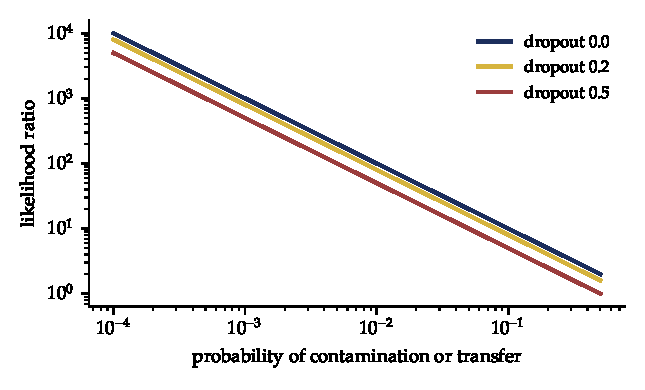
\includegraphics[width=\linewidth]{fig_lowtemplate}
\caption{Bayes factor for a low template DNA detection as a function of the probability of innocent transfer or contamination, for a profile with random match probability $10^{-9}$, at three drop out rates.}
\label{fig:lowtemplate}
\end{figure}

\section{The database search controversy}

Chapter~\ref{ch:classic} worked the search version of the island problem. When a suspect is found by searching a database of profiles, rather than by investigation, does the search weaken the evidence? The second National Research Council report recommended multiplying the match probability by $n$, the number of profiles in the database, on the analogy of a multiple comparisons correction \citep{nrc1996}. Balding and Donnelly argued the opposite, that a database search slightly strengthens the case against the matching individual, because it eliminates the other people in the database as possible sources \citep{balding2005}.\index{database search}

The Bayesian analysis clarifies the question, provided one is careful about the hypothesis. If the question is whether the matching individual is the source, the relevant likelihood ratio is still about $1/\gamma$, and the search has excluded $n-1$ people from the pool of alternatives, so the posterior odds rise slightly. If the question is whether the database contains the source at all, the probability of finding at least one match by chance is about $n\gamma$, and the frequentist correction answers that question. The two camps were answering different questions. What matters is the prior: a person found by trawling a database usually has no other evidence against him, so the prior is the uniform $1/N$ of the island problem of Chapter~\ref{ch:odds}, with $N$ the number of people who could be the source, the defendant included, while a person found by investigation may have a much higher prior. The danger in cold hit cases is not that the likelihood ratio is wrong but that the prior is low and the rest of the case is thin.

\section{Bayes factors and p values}

Statistical evidence in discrimination cases, in antitrust, and in many regulatory disputes is often presented through significance tests. In \emph{Castaneda v Partida} and \emph{Hazelwood School District v United States}, both decided by the United States Supreme Court in 1977, the Court suggested that a disparity of more than two or three standard deviations between the observed and expected numbers of a group would raise suspicion of discrimination \citep{castaneda1977,hazelwood1977}. Lower courts have since often treated a p value below five per cent as a threshold. Chapter~\ref{ch:fienberg} discusses \emph{Castaneda} in detail.\index{p value}\index{Castaneda v Partida}

A p value is not a Bayes factor and not a probability that the null hypothesis is true. For a point null hypothesis tested against a range of alternatives, the Bayes factor implied by a given p value depends on the sample size and on the prior for the alternative. Sellke, Bayarri and Berger showed that, under broad conditions, the Bayes factor in favour of the alternative cannot exceed
\begin{equation}
\overline{\BF}(p) = \frac{-1}{e\, p\log p}, \qquad p < 1/e,
\label{eq:sbb}
\end{equation}
with $\log$ the natural logarithm, which for $p = 0.05$ is about $2.5$ and for $p = 0.01$ is about $8$ \citep{sellke2001}. A result that just reaches conventional significance therefore provides at most modest evidence against the null, rarely enough by itself to meet even a civil standard unless the prior odds are close to even. Conversely, a small p value in a large sample can be paired with weak or even contrary Bayes factors, which is the phenomenon Lindley identified.\index{Sellke Bayarri Berger bound}

\section{Lindley's paradox}

Lindley's paradox concerns a point null hypothesis $H_0 : \theta = 0$ tested against $H_1 : \theta \sim N(0,\tau^2)$, with data summarised by a sample mean whose standard error is $1/\sqrt{n}$. Suppose the observed $z$ statistic is fixed at two, just significant at the five per cent level. The Bayes factor in favour of the null is
\begin{equation}
\BF_{01} = \sqrt{1 + n\tau^2}\,\exp\left(-\frac{z^2}{2}\frac{n\tau^2}{1+n\tau^2}\right),
\label{eq:lindleybf}
\end{equation}
which grows without bound as $n$ increases \citep{lindley1957}. A result that is significant at five per cent in a large sample becomes strong evidence for the null against a diffuse alternative as $n$ grows. Figure~\ref{fig:lindley} shows the Bayes factor as $n$ grows.\index{Lindley's paradox}

\begin{figure}[t]
\centering
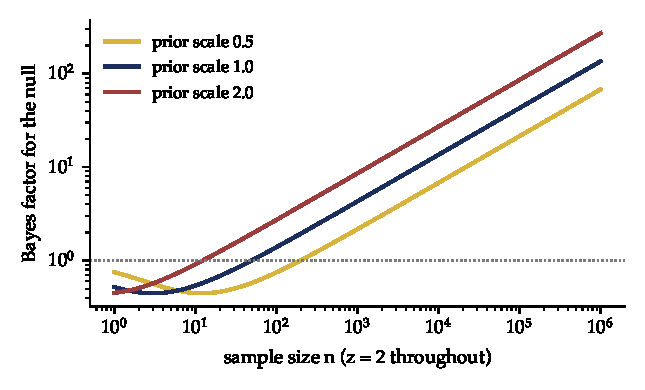
\includegraphics[width=\linewidth]{fig_lindley}
\caption{Lindley's paradox. With the $z$ statistic held at two, the Bayes factor in favour of the null hypothesis grows with the sample size, for each of three prior scales on the alternative.}
\label{fig:lindley}
\end{figure}

The paradox matters in litigation because modern cases often involve large data sets: millions of transactions in a price fixing case, every hiring decision of a national employer, all the trades in a market manipulation inquiry. In such cases trivial deviations from a null hypothesis become statistically significant. The question the court must answer is not whether the deviation is zero but whether it is large enough to matter, and whether the claimant's account predicts the data better than the defendant's. A Bayes factor comparing two substantively specified hypotheses, for instance a hiring rate equal to the qualified labour pool against a rate reduced by a meaningful margin, answers that question directly.

\section{Sensitivity and robustness}

The objection to Bayes factors most often heard in court is that they depend on priors for parameters, and so are subjective. The answer is that the dependence should be reported, not hidden. A forensic report or an expert's evidence should show the Bayes factor over a range of reasonable priors, and the conclusion should be stated in terms that hold across that range. If the Bayes factor exceeds one thousand for every prior an informed person could reasonably hold, the evidence is strong; if it ranges from two to two thousand, the report should say so, and the fact finder must weigh the expert's reasons for preferring one end.\index{robustness}

There is a formal theory of such ranges. Robust Bayesian analysis computes the infimum and supremum of the posterior or the Bayes factor over a class of priors, such as all priors within a given distance of a reference prior or all priors with specified quantiles \citep{berger1994}. For legal use the classes should be defined by what the parties can argue about: the population frequency of a feature, the error rate of a laboratory, the prior probability that a defendant had access to an item. The resulting interval of Bayes factors is a natural thing for an expert to report.

\begin{casebox}{A worked example: footwear marks}
A shoe print at a scene matches the defendant's shoe in pattern, size and two wear features. Suppose the pattern is shared by between one and five per cent of shoes in circulation, the size by about ten per cent of shoes of that pattern, and each wear feature by between five and twenty per cent of shoes of that pattern and size, independently. The Bayes factor lies between
\begin{gather*}
\frac{1}{0.05\times 0.1 \times 0.2 \times 0.2} = 5{,}000 \quad\text{and}\quad\\ \frac{1}{0.01\times 0.1\times 0.05\times 0.05} = 400{,}000 .
\end{gather*}
Even the lower bound is strong evidence that the shoe made the mark. In \emph{R v T} the expert gave a verbal conclusion that rested on an undisclosed likelihood ratio, computed from frequency data that the Court of Appeal found unreliable \citep{rvt2010}; Chapter~\ref{ch:odds} describes the case. Stating the inputs and their ranges answers the concern about transparency, while whether the footwear database can support any such figure remains a matter of argument \citep{berger2011}.
\end{casebox}

\section{Hierarchical models for forensic frequencies}

Many forensic frequencies are estimated from small databases. A glass fragment's refractive index, a fibre's dye, a toolmark's striations: each is compared with a reference collection of modest size. The uncertainty in the frequency is then substantial, and the Bayes factor should reflect it. If the observed count of a feature in a database of size $n$ is $k$, and the frequency $\gamma$ has a beta prior $\text{Beta}(a,b)$, the predictive probability that a new random item shares the feature is
\begin{equation}
\Prob(\text{match}\given k,n) = \frac{k + a}{n + a + b},
\label{eq:betapred}
\end{equation}
which for $k = 0$ gives $a/(n+a+b)$ rather than zero. This simple formula is the Bayesian answer to the frequent embarrassment of a feature never before seen in a database. With a uniform prior, $a = b = 1$, a feature unseen in a database of one hundred has predictive frequency about one per cent; once the suspect's own item is counted as a further observation the conditional match probability is $2/103$, and the Bayes factor is about fifty, not infinity.\index{hierarchical model}

When features come from several populations, a hierarchical model pools information across them while allowing each its own frequency. This is the structure of the subpopulation correction in DNA statistics, where the parameter $\theta$, often called $F_{ST}$, measures the excess relatedness within a subpopulation. The Balding and Nichols formula for the conditional match probability of a heterozygote,
\begin{equation}
\Prob(\text{match}) = \frac{2\,[\theta + (1-\theta)p_a][\theta + (1-\theta)p_b]}{(1+\theta)(1+2\theta)},
\end{equation}
is the predictive probability under a Dirichlet model for allele frequencies in the subpopulation \citep{balding2005}.

\section{Bayes factors for stories and theories}

The Bayes factor applies to any pair of hypotheses that make predictions, not just to forensic identification. In civil litigation the competing hypotheses are often whole theories of what happened: that a company knew of a defect and concealed it, or that it discovered the defect only later; that a trader manipulated a benchmark, or that his submissions reflected his honest view of the market. Each theory predicts the documents, emails and trading records, and the Bayes factor measures which theory predicts them better. Chapter~\ref{ch:stories} develops this idea as a theory of legal stories.

A useful way to think of a composite theory is as a mixture over subplots. The claimant's theory $\Hp$ is a set of possible histories, each with a prior weight; its marginal likelihood is the weighted average of the probability of the evidence under each history. A theory that fits the evidence only under a narrow set of improbable assumptions has a low marginal likelihood, because the assumptions carry little prior weight. This is the Bayesian form of Occam's razor, and it sits naturally with Lord Brandon's warning in \emph{The Popi M} that a judge is not bound to choose between two improbable explanations \citep{popim1985}. A court may conclude that neither party's account is probable enough to discharge the burden.

\section{Communicating Bayes factors}

Fienberg and Kadane, writing in 1983, set out principles for presenting Bayesian analyses in legal proceedings \citep{fienberg_kadane1983}. The analyst should state the model and the prior clearly, show the results under the priors that the opposing party is likely to favour, and avoid presenting a single posterior probability of guilt, which usurps the role of the fact finder. Over forty years later these principles remain sound. We would add three more. First, report the Bayes factor on the log scale as well as the natural scale, because people find additive weights easier to compare than multiplicative factors. Second, distinguish the source question, whose trace this is, from the activity question, how the trace got there, and report a Bayes factor only for the question it actually addresses. Third, give the fact finder a picture, such as Figure~\ref{fig:posterior} here and Figure~\ref{fig:population} of Chapter~\ref{ch:odds}, which show the posterior over a range of priors, so that the consequences of their own judgments are visible.

\begin{figure}[t]
\centering
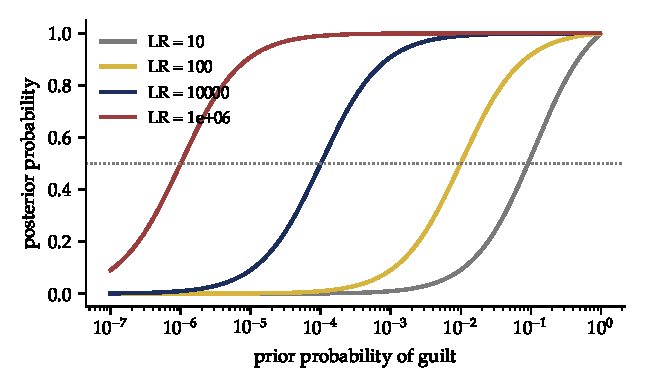
\includegraphics[width=\linewidth]{fig_posterior_odds}
\caption{Posterior probability as a function of the prior probability for four likelihood ratios. A Bayes factor of a million moves a prior of one in a hundred thousand to about $0.9$; a factor of one hundred leaves it close to zero.}
\label{fig:posterior}
\end{figure}

\section*{Notes and Questions}
\addcontentsline{toc}{section}{Notes and Questions}
\begin{enumerate}[label=\arabic*.]
\item Derive \eqref{eq:dnaerror} from a model in which a reported match occurs either because the profiles truly match or because of laboratory error. Under what conditions is the approximation poor?
\item Evaluate \eqref{eq:sbb} for $p = 0.05, 0.01, 0.001$. Compare these bounds with the posterior probabilities a court might mistakenly read off from the p values.
\item Using \eqref{eq:lindleybf} with $\tau = 1$, find the sample size at which a $z$ statistic of $2.5$ becomes evidence for the null.
\item A fibre type is absent from a database of $250$ garments. Using \eqref{eq:betapred}, with the suspect's own item counted as a further observation, and $a = b = 1$, compute the Bayes factor for a match. Repeat with $a = 0.5$, $b = 0.5$.
\item In the footwear casebox, suppose the two wear features are positively correlated, so that given the first the probability of the second doubles. Recompute the bounds.
\item Construct an example of two composite theories in a civil case, specify priors over their subplots, and compute the marginal likelihoods of a set of three documents. Explain how the Bayesian Occam factor appears.
\end{enumerate}

\section*{Further reading}
Kass and Raftery's review remains the best introduction to Bayes factors \citep{kass1995}. On robustness see Berger \citep{berger1994}. On DNA, Balding \citep{balding2005} and the NRC report \citep{nrc1996}. Thompson's work on laboratory error is essential reading \citep{thompson2003}.

\chapter{Fallacies of Classical Inference}
\label{ch:fallacies}

\section{Significance in the courtroom}

Most statistical evidence presented in courts is classical. Experts report p values, significance levels, confidence intervals and standard deviations, the vocabulary of the frequentist statistics that dominated the twentieth century. Michael Finkelstein, a lawyer who did much to bring statistics into American legal education, built his casebooks, \emph{Quantitative Methods in Law} and, with the biostatistician Bruce Levin, \emph{Statistics for Lawyers}, around this vocabulary, because it is the vocabulary courts encounter \citep{finkelstein2015}. Finkelstein was also, with William Fairley, the author of the 1970 proposal to show juries Bayesian calculations that provoked Tribe's reply, discussed in Chapter~\ref{ch:why} \citep{finkelstein1970}. His casebook is an essential companion to this one: it teaches the methods courts actually see, with hundreds of problems drawn from real cases. Our concern in this chapter is with what happens when those methods are misread, and with cases in which a Bayesian analysis of the same data leads to a different conclusion.\index{Finkelstein, Michael}\index{classical inference}

We identify ten fallacies, each common in litigation. For each we state the fallacy, explain why it is an error, and give an example in which a Bayesian analysis would overturn the classical reading. The examples are constructed to be realistic, and some follow the pattern of decided cases.

\section{1. The p value is the probability that the null is true}

\paragraph{The fallacy} An expert reports that a disparity has a p value of $0.01$, and counsel tells the court that there is only a one per cent chance the disparity is due to chance, so a ninety nine per cent chance of discrimination.

\paragraph{Why it is wrong} The p value is the probability, assuming the null hypothesis, of data at least as extreme as those observed. It is $\Prob(\text{data this extreme}\given H_0)$, not $\Prob(H_0\given\text{data})$. The error is the prosecutor's fallacy of Chapter~\ref{ch:odds} in a different setting. The posterior probability of the null depends on its prior probability and on how probable the data are under the alternatives, neither of which the p value addresses.

\paragraph{Bayes overturns} By the Sellke, Bayarri and Berger bound \citep{sellke2001} of Chapter~\ref{ch:bf} (equation~\eqref{eq:sbb}), a p value of $0.01$ corresponds to a Bayes factor against the null of at most about eight. If the prior probability of discrimination, given the employer's practices and the industry, is one in five, the posterior probability is at most $8\times 0.25/(1 + 8\times 0.25) = 2/3$, not ninety nine per cent. With a prior of one in twenty, the posterior is at most about thirty per cent. A finding that would be presented as near certain is, on a coherent reading, wrong at least one time in three, and with the lower prior more likely than not.

\section{2. Not significant means no effect}

\paragraph{The fallacy} A small study finds that patients taking a drug suffered a serious adverse event at three times the rate of controls, but the difference is not statistically significant. The defendant argues, and a court accepts, that there is no evidence the drug causes the event.

\paragraph{Why it is wrong} Failure to reject a null hypothesis is not evidence for it. A small study has low power; even a real and large effect will often fail to reach significance. Absence of significance is absence of a particular kind of proof, not proof of absence.

\paragraph{Bayes overturns} Suppose six of one hundred patients on the drug and two of one hundred controls suffered the event. Fisher's exact test gives a two sided p value of about $0.28$, far from significant. With uniform priors on the two event rates, the posterior probability that the rate on the drug exceeds the rate on placebo is about $0.91$, and the posterior probability that the relative risk exceeds two is about $0.62$. The data favour a harmful effect, substantially. A court asking whether the evidence makes harm more probable than not, the civil question, should answer yes, even though no significance test was passed.\index{statistical significance}

\begin{casebox}{Matrixx Initiatives v Siracusano, 563 U.S. 27 (2011)}
Investors sued a company that sold a zinc based cold remedy, alleging that it had failed to disclose reports that users had lost their sense of smell. The company argued that the reports were not material because they did not establish a statistically significant association. The Supreme Court unanimously rejected a bright line rule requiring statistical significance for materiality. Medical professionals and regulators, the Court observed, act on evidence that is not statistically significant and that suggests but does not prove causation, and reasonable investors would too. The decision is a judicial recognition of the second fallacy \citep{matrixx2011}.
\end{casebox}

The First Circuit's decision in \emph{Milward v Acuity Specialty Products}, which accepted an expert's weight of evidence methodology for inferring that benzene exposure can cause a rare leukaemia despite the paucity of statistically significant epidemiological studies, rests on the same insight \citep{milward2011}. Evidence accumulates from many sources, none of which need be significant on its own.

\section{3. Significant means important}

\paragraph{The fallacy} In a large employment dataset, the promotion rate for one group is $29.7$ per cent and for another $30.0$ per cent. With a million employees in each group, the difference is about four and a half standard errors from zero, highly significant. The claimant argues that the employer's promotion system is discriminatory.

\paragraph{Why it is wrong} Statistical significance measures whether a difference can be distinguished from zero, not whether it matters. With enough data, any nonzero difference becomes significant. The ratio of promotion rates here is $0.99$, far above the four fifths guideline, under which a group's selection rate below four fifths of the most favoured group's rate is taken as evidence of adverse impact; Chapter~\ref{ch:discrimination} returns to it.

\paragraph{Bayes overturns} A Bayesian analysis compares substantively specified hypotheses: no meaningful disparity, say a ratio above $0.95$, against meaningful disparity, a ratio below $0.95$. With a million observations per group, the posterior for the ratio is concentrated within a fraction of a per cent of $0.99$, and the posterior probability of a meaningful disparity is negligible. The same data that are highly significant against exact equality are overwhelming evidence against discrimination of any practical size. This is the large sample problem behind Lindley's paradox, discussed in Chapter~\ref{ch:bf}, applied to a discrimination claim.

\section{4. The confidence interval contains the parameter with ninety five per cent probability}

\paragraph{The fallacy} An expert reports a ninety five per cent confidence interval for damages of four to twelve million, and the court treats this as a ninety five per cent probability that damages lie in that range.

\paragraph{Why it is wrong} In classical theory, the parameter is fixed and the interval random. The ninety five per cent describes the procedure: in repeated samples, ninety five per cent of intervals so constructed would contain the parameter. It does not describe the probability that this interval does. In simple problems with flat priors the Bayesian credible interval and the confidence interval coincide numerically, and the misreading is harmless. In other problems they differ.

\paragraph{Bayes overturns} Suppose an overcharge is estimated from a small number of cartel transactions, with a confidence interval of minus two to ten per cent. A negative overcharge, a cartel that lowered prices, is economically implausible. A Bayesian analysis with a prior that puts negligible weight on negative overcharges gives a credible interval of perhaps one to ten per cent and a posterior median of five per cent, while the confidence interval, read naively, suggested that zero was a plausible value. The court that reads ``the interval contains zero'' as showing no overcharge, which is the error of the second fallacy, would wrongly conclude that the claimant had not shown an overcharge to be more likely than not. The gain here comes from the informative prior, not from reading the interval as a probability statement, which for a flat prior would be harmless.

\section{5. Multiple comparisons ignored}

\paragraph{The fallacy} An expert examines a company's pay data by department, job grade, year and protected characteristic, runs a hundred comparisons, and presents the five that are significant at the five per cent level as evidence of discrimination.

\paragraph{Why it is wrong} With a hundred independent comparisons and no discrimination at all, about five would be significant by chance. Selecting the significant ones and presenting them without the others is the Texas sharpshooter fallacy, drawing the target around the bullet holes after firing, to which Chapter~\ref{ch:clusters} returns. Classical corrections such as Bonferroni's divide the significance level by the number of tests; they are crude but recognise the problem.

\paragraph{Bayes overturns} A hierarchical model treats the hundred department level disparities as draws from a common distribution, estimates its mean and variance, and shrinks each department's estimate toward the mean. If the overall mean is close to zero and the between department variance is small, the five apparently significant departments are shrunk nearly to zero, and their posterior probabilities of real disparity are modest. If, instead, the model finds a negative overall mean with tight variance, the evidence is of a firm wide pattern, stronger than any single comparison. Either way, the hierarchical analysis answers the right question, whether there is discrimination and where, rather than whether some comparisons cross a threshold.\index{multiple comparisons}

\section{6. The stopping rule matters}

\paragraph{The fallacy} An auditor samples transactions until three errors are found, which happens after twelve transactions. A second auditor samples exactly twelve transactions and finds three errors. Classical analysis gives them different p values for the hypothesis that the error rate is one half or more: the first auditor's design yields one, the second auditor's another, because the probability of more extreme outcomes depends on what the auditor would have done.

\paragraph{Why it is wrong} The two auditors observed the same data. The likelihood function for the error rate is the same, proportional to $\theta^3(1-\theta)^9$, whichever design was used. The likelihood principle, which follows from Bayesian reasoning, says that inferences should depend on the data only through the likelihood. A legal conclusion that depends on what an auditor intended to do, rather than on what she observed, is hard to defend.

\paragraph{Bayes overturns} Take the textbook case of nine successes and three failures (the failures being the errors of the audit). Under a fixed sample of twelve, the one sided p value against a rate of one half is about $0.073$, not significant. Under sampling until three failures, it is about $0.033$, significant. Two experts could reach opposite conclusions from the same data. The Bayesian posterior for the rate, with any given prior, is the same in both cases. A court relying on the classical analysis would decide differently depending on an unrecorded intention; a Bayesian court would not.\index{likelihood principle}\index{stopping rule}

\section{7. Two or three standard deviations}

\paragraph{The fallacy} Following \emph{Castaneda} and \emph{Hazelwood} \citep{castaneda1977,hazelwood1977}, a court treats any disparity of more than two or three standard deviations as establishing a prima facie case of discrimination, and anything less as insufficient.

\paragraph{Why it is wrong} The number of standard deviations measures how surprising the data would be under random selection, but not how much more probable they are under discrimination. In a small sample, a substantial and real disparity may fall short of two standard deviations; in a large sample, a trivial one will exceed three.

\paragraph{Bayes overturns} A small employer has hired twenty people from a pool that is thirty per cent women and has hired two women. The expected number is six with a standard deviation of about two; two is just under two standard deviations below, borderline. With a prior that if the employer discriminates its effective rate of hiring women is uniformly distributed between zero and the pool share, the Bayes factor for discrimination is about five and a half. In combination with other evidence, such as remarks by the hiring manager, that may well carry a civil claim. Conversely, in a national dataset, a disparity of four standard deviations may correspond to a hiring ratio of $0.97$, with a Bayes factor favouring the absence of any meaningful discrimination. The standard deviation rule decides both cases wrongly.

\section{8. One tail or two}

\paragraph{The fallacy} An expert chooses a one tailed test, which halves the p value, after seeing which direction the data point, and reports significance.

\paragraph{Why it is wrong} The choice between one and two tailed tests is a choice about which alternatives are entertained, and it must be made before seeing the data. Choosing after the fact is a form of selection. Courts have argued about tails for decades, and Finkelstein and Levin discuss the cases \citep{finkelstein2015}.

\paragraph{Bayes overturns} In a Bayesian analysis the question does not arise. The prior over the alternatives says which directions are plausible; if a disparity favouring the protected group is implausible, the prior gives it low weight, and the analysis is in effect one sided, but openly so and fixed before the data. The Bayes factor does not change when an expert changes his mind about tails.

\section{9. Combining p values}

\paragraph{The fallacy} An expert combines evidence from several sources by multiplying their p values, or by Fisher's method, and reports an astronomically small combined p value.

\paragraph{Why it is wrong} Multiplying p values does not produce a p value; the product of uniformly distributed quantities is not uniform. Fisher's method correctly combines independent p values into a test of the global null, but it tests only whether at least one source departs from the null, not whether the combined evidence favours a particular alternative. Neither method accounts for dependence between sources or for how they were selected. The case of Lucia de Berk, a Dutch nurse convicted of murdering patients and later exonerated, to which Chapter~\ref{ch:clusters} returns, turned partly on an improper combination of p values across wards.

\paragraph{Bayes overturns} Bayes factors for independent items multiply; their logarithms add. This is the correct way to combine evidence, and it requires each item's likelihood ratio, not its p value. In the de Berk case, reanalyses of the association between the nurse's shifts and incidents, accounting for the selection of incidents and for the heterogeneity between wards, found far weaker evidence than the combined p value suggested \citep{meester2006,gill2018}. Those reanalyses were classical, recomputing corrected p values; a likelihood ratio analysis would go further.

\section{10. Testing without an alternative}

\paragraph{The fallacy} An analysis rejects the hypothesis of innocence because the evidence is improbable under it, without asking how probable the evidence is under guilt.

\paragraph{Why it is wrong} Every observation is improbable under some hypothesis. A particular shuffled deck of cards has probability one in $52!$, yet no one infers that the shuffle was rigged. Evidence supports guilt only if it is more probable under guilt than under innocence. A significance test that considers only the null cannot tell whether the data favour the alternative.

\paragraph{Bayes overturns} In \emph{People v Collins} \citep{collins1968}, treated in Chapter~\ref{ch:odds}, the prosecutor's probability of one in twelve million for the characteristics of a random couple was presented as if it showed guilt. A Bayesian analysis asks how probable it is that the guilty couple has those characteristics, near one if the description is accurate, and how many innocent couples share them, the island problem. The answer, as the California Supreme Court saw, did not support conviction. Every case in Chapter~\ref{ch:classic} is a case in which asking about the alternative changes the conclusion.

\section{Why the fallacies persist}

These fallacies are not the result of ignorance on the part of statisticians; most are discussed in most introductory textbooks. They persist in litigation for institutional reasons. Courts have adopted significance thresholds as rules of thumb, and experts who depart from them must explain why. Classical methods appear objective, because they do not require a prior, while Bayesian methods appear subjective. And the adversarial system rewards experts whose analyses favour their clients, which the flexibility of classical procedures, the choice of tests, tails, subgroups and stopping rules, makes easy to provide.

The Bayesian answer to the objectivity concern is that the prior is not hidden in classical methods but absent, and its absence is what produces the fallacies. A p value of five per cent means different things in a case where discrimination is common and in one where it is rare, and a method that ignores the difference is not objective but blind. The remedy is to make the prior explicit, show how the conclusion depends on it, and let the court judge. That is what Fienberg and Kadane recommended in 1983 \citep{fienberg_kadane1983}, and what Finkelstein and Fairley proposed in 1970. The courts have been slow to listen, but \emph{Matrixx} shows that they can abandon a rigid significance rule.

\section*{Notes and Questions}
\addcontentsline{toc}{section}{Notes and Questions}
\begin{enumerate}[label=\arabic*.]
\item Using the Sellke, Bayarri and Berger bound, find the maximum posterior probability of the alternative for a p value of $0.05$ when the prior probability is one half, one fifth and one twentieth.
\item In the adverse event example, compute the posterior probability that the relative risk exceeds two under a prior that puts half its mass on no effect and half on a uniform relative risk between one and five, and a uniform prior on the placebo rate.
\item Show that the likelihoods for nine successes and three failures under binomial and negative binomial sampling are proportional. Why does the classical p value differ?
\item Read \emph{Matrixx Initiatives v Siracusano}. Which other fallacies in this chapter does the Court's reasoning address?
\item Construct a dataset with a hundred department level comparisons in which a hierarchical model finds a firm wide disparity although no single department is significant.
\item Choose a problem from Finkelstein and Levin's \emph{Statistics for Lawyers}. Solve it classically and with Bayesian methods. Do the conclusions differ? Why?
\end{enumerate}

\section*{Further reading}
Finkelstein and Levin's \emph{Statistics for Lawyers} \citep{finkelstein2015}; Finkelstein and Fairley \citep{finkelstein1970}; Sellke, Bayarri and Berger \citep{sellke2001}; Lindley's paradox \citep{lindley1957}.

\chapter{Standards of Proof as Decision Rules}
\label{ch:standards}

\section{Two standards and one theory}

English law knows two standards of proof. In criminal cases the prosecution must make the jury sure of guilt, the modern form of proof beyond reasonable doubt. In civil cases the claimant must prove the facts on the balance of probabilities, which means that the fact is more probable than not. American law adds an intermediate standard, clear and convincing evidence, for matters such as fraud, civil commitment and the termination of parental rights. Civil law systems state their standards differently, as we shall see in Chapter~\ref{ch:commoncivil}, but they too distinguish criminal from civil proof.\index{standard of proof}

Decision theory explains these standards as thresholds on the posterior probability, each determined by the ratio of the losses from the two kinds of error. Equation \eqref{eq:threshold} gave the threshold, which we write here as $p^\ast = L_{FC}/(L_{FC} + L_{FA})$, where $L_{FC} = L(c,\bar G)$ is the loss from a false conviction, or more generally a false finding for the party bearing the burden, and $L_{FA} = L(a,G)$ the loss from a false acquittal. John Kaplan set out this analysis in 1968, and it has been refined many times since \citep{kaplan1968,kaye1999}. The civil standard corresponds to equal losses, $p^\ast = 1/2$. The criminal standard corresponds to a ratio of losses of perhaps ten or twenty to one, $p^\ast$ between about $0.9$ and $0.95$. The intermediate standard corresponds to an intermediate ratio.

The theory is simple. Its consequences are not. This chapter works through them: what the threshold implies about the meaning of reasonable doubt, how it interacts with the seriousness of the allegation, what it says about naked statistical evidence, and how Lindley used it to argue for graduated sanctions.

\section{What judges think reasonable doubt means}

Courts have generally refused to quantify reasonable doubt, and juries are told not to think in percentages. Yet when judges have been asked to translate the standard into a probability, their answers cluster. In \emph{United States v Fatico}, Judge Jack Weinstein reported an informal survey of his colleagues in the Eastern District of New York: their numerical equivalents for proof beyond reasonable doubt ranged from about three quarters to about ninety five per cent, with most near the upper end, and those for clear and convincing evidence clustered between about sixty and seventy five per cent \citep{fatico1978}. Surveys of jurors and students find wider dispersion and, worryingly, some respondents who place the criminal standard below the civil one. The dispersion matters. If one jury convicts at $0.75$ and another at $0.95$, the implied ratio of losses varies from three to nineteen, which is a large difference in the value the system places on avoiding false convictions.\index{reasonable doubt}

There is a principled reason courts avoid numbers: a fact finder who is told that ninety per cent suffices may treat a case at ninety per cent as a conviction, while one told only to be sure may hold out for more. Numbers can act as anchors. But the absence of numbers does not remove the threshold; it makes it invisible and variable. A Bayesian analysis cannot tell a society what ratio of losses to adopt. It can tell a society what ratio its procedures are in fact implementing, and whether that ratio is consistent across courts.

\section{The value of a correct decision depends on the stakes}

The simple threshold treats losses as fixed. In fact they vary with the seriousness of the charge, the severity of the sentence and the collateral consequences of conviction. A false conviction for murder is worse than a false conviction for shoplifting; so is a false acquittal. The threshold depends on their ratio, which need not change in any particular direction as seriousness increases. Some scholars argue, without agreement, that the criminal standard should rise with the sentence; others that it should fall for the gravest crimes, where the harm of a false acquittal is large. English law takes neither view for criminal cases: the standard is the same for all offences.\index{seriousness of allegation}

For civil cases the English courts went through a period of confusion. In \emph{Re H (Minors)} Lord Nicholls said that the more serious the allegation, the less likely it is that the event occurred, and hence the stronger the evidence needed before the court concludes that it is established on the balance of probabilities \citep{reh1996}. Lower courts read this as raising the standard for serious allegations. In \emph{Re B (Children)} the House of Lords corrected the reading: there is one civil standard, the balance of probabilities, and the seriousness of an allegation is relevant only so far as it bears on the inherent probability of the event \citep{reb2008}.

The Bayesian reading makes the distinction exact. Lord Nicholls was talking about the prior. Serious wrongdoing, such as the sexual abuse of a child or a fraud on a large scale, is usually rarer than minor wrongdoing, so its prior probability is lower, and more evidence is required to bring the posterior above one half. That is not a change in the threshold; it is a change in the starting point. Lady Hale in \emph{Re B} added that there is no necessary connection between seriousness and improbability, and Lord Hoffmann gave the example: if a child has been injured by one of only two people, it makes no sense to reason that injuring a child is serious and so neither is likely to have done it, since one of them did. The posterior threshold remains one half, and the prior is what it is. This is close to the Bayesian theory of the civil standard.

\section{Burden and prior}

The burden of proof says which party loses if the evidence leaves the fact finder at the threshold or below it. In decision terms it assigns the default action. The presumption of innocence is the criminal burden, but it has often been read as something stronger, a requirement that the fact finder begin with a prior probability of guilt of zero, or at least a small one. As we noted in Chapter~\ref{ch:why}, a prior of zero cannot be updated. The best Bayesian reading is that the defendant should be treated, before evidence specific to him is considered, as an exchangeable member of the population of people who could have committed the crime. If that population has $N$ members, his prior probability of guilt is $1/N$. Philip Dawid and others have defended this reading \citep{dawid2002}.\index{presumption of innocence}

The $1/N$ prior has attractive features. It does not depend on the fact that the defendant has been charged, which would be circular, since the charge reflects the evidence. It treats the defendant as an ordinary person. And it makes the role of evidence transparent: a conviction requires evidence whose combined Bayes factor exceeds roughly $N \cdot p^\ast/(1-p^\ast)$. For a crime that anyone in a city of a million could have committed and a threshold of $0.95$, this is about nineteen million, or seventy three decibans. A single DNA match with a random match probability of one in a billion and no error supplies ninety decibans and would suffice; on some estimates a single eyewitness supplies perhaps ten. Most convictions rest on many items of moderate weight that together cross the threshold.

\section{The gatecrasher and the expected utility solution}

Jonathan Cohen posed the gatecrasher problem in 1977 \citep{cohen1977}. At a rodeo 499 people pay for admission but 1{,}000 are counted in the seats; no tickets are issued, so nobody can show whether a given person paid. The organiser sues a randomly chosen attendee for the price of admission. With no other evidence, the probability that this person gatecrashed is $501/1000$, just over one half. On the balance of probabilities the organiser should win, and could win against every attendee, recovering $1{,}000$ admission fees when only $501$ are owed. Cohen used the example to argue that legal proof is not governed by the mathematical calculus of probability, and proposed an inductive, Baconian probability in its place.\index{gatecrasher paradox}

Several responses have been offered. One is that the probability is not really $0.501$, because, if tickets were issued (which departs from Cohen's stipulation), a ticket holder would usually keep the stub, and the defendant's failure to produce one is evidence. Another is that liability on naked statistics creates bad incentives, as in the blue bus case (Chapter~\ref{ch:odds}). Lindley took up the problem in his 1991 paper and offered a new solution within decision analysis \citep{lindley1991}. The solution we find most persuasive, in the spirit of that paper, starts from the observation that the paradox arises from forcing the court into an all or nothing choice. If the court could award damages equal to the probability of liability times the loss, it would award each attendee $0.501$ of the admission price, and the organiser would recover in total $501$ admission fees, exactly what it was owed. The expected utility solution reproduces the correct aggregate result, though not individual justice, since each of the 499 who paid is still charged $0.501$ of the fee. The paradox is a symptom of the binary system, not of probability.

The point generalises. Whenever the law insists on all or nothing remedies, it creates discontinuities at the threshold, and those discontinuities generate both injustice in individual cases and perverse incentives in the aggregate. Proportional remedies smooth the discontinuity (Figure~\ref{fig:losschance}). English law has accepted proportional damages in some contexts, notably loss of a chance in contract and professional negligence cases such as \emph{Allied Maples v Simmons and Simmons}, and refused it in others, notably in clinical negligence in \emph{Gregg v Scott} \citep{alliedmaples1995,gregg2005}. Chapter~\ref{ch:tort} examines these cases in detail.

\begin{figure}[t]
\centering
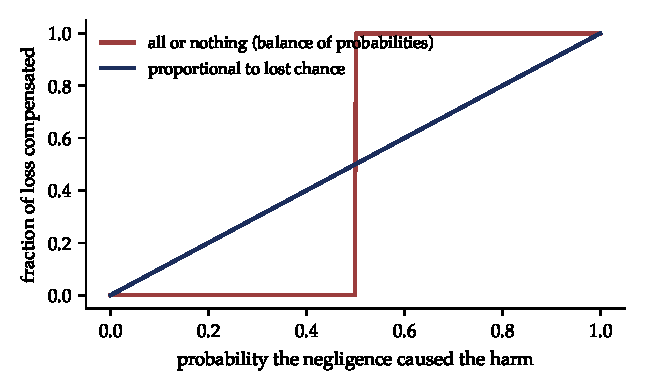
\includegraphics[width=\linewidth]{fig_loss_chance}
\caption{Compensation as a function of the probability that the defendant's breach caused the loss, under the all or nothing rule of the balance of probabilities and under proportional liability. The first has a jump at one half; the second is continuous.}
\label{fig:losschance}
\end{figure}

\section{Graduated sanctions}

Lindley also applied expected utility to criminal sentencing. Suppose the court can choose among acquittal, a light sentence and a heavy sentence, and suppose the losses are as in Table~\ref{tab:sanctions}. A light sentence imposed on an innocent person is a harm, but a smaller harm than a heavy one; a light sentence imposed on a guilty person is an under punishment, but less of a loss than an acquittal. Then for a middle range of posterior probabilities the light sentence minimises expected loss. In particular, there may be a range of probabilities below the conventional threshold for which some sanction is optimal \citep{lindley1991}.

\begin{table}[t]
\centering
\small
\begin{tabular}{lcc}
\toprule
Action & Loss if innocent & Loss if guilty\\
\midrule
Acquit & 0 & 10\\
Light sanction & 20 & 4\\
Heavy sanction & 100 & 0\\
\bottomrule
\end{tabular}
\caption{An illustrative loss table for three actions. Expected losses are $10p$, $20(1-p) + 4p$ and $100(1-p)$. Acquittal is optimal for $p < 0.77$, the light sanction for $0.77 < p < 0.95$, and the heavy sanction above.}
\label{tab:sanctions}
\end{table}

This conclusion is uncomfortable, and Lindley knew it. It conflicts with the principle that no one should be punished unless proved guilty, a principle that is constitutive of the criminal law rather than an instrumental rule. The Bayesian can respond that the principle is itself a statement about utilities: society may attach a large disutility to any punishment of a person not proved guilty, beyond the direct harm of the punishment, because such punishment undermines trust in law. If that disutility is large enough (in Table~\ref{tab:sanctions}, at least $100$), the light sanction disappears from the optimal set altogether. The framework accommodates the principle; it asks that its cost be made explicit. In practice the criminal law has many graduated responses that operate below the full criminal standard: bail conditions, protective orders, civil recovery, and regulatory sanctions. The decision theoretic view helps organise these and ask whether their thresholds are consistent.

\section{The value of information and when to stop}

A court does not only decide; it decides when to decide. Adjournments, further disclosure, expert reports and retrials all buy information at a cost. The expected value of sample information is the reduction in expected loss from the decision that the new information makes possible, before the information is seen. If the posterior is already far from the threshold, new evidence is unlikely to change the decision and is worth little. If the posterior is near the threshold, even modest evidence may tip it, and its value is high.\index{value of information}

Formally, let the current posterior be $p$ and suppose a further item of evidence would have Bayes factor $B$ with known distribution under each hypothesis. The value of obtaining it is
\begin{equation}
\mathrm{VOI}(p) = \min\{p L_{FA}, (1-p)L_{FC}\} - \E\left[\min\{p' L_{FA}, (1-p') L_{FC}\}\right],
\end{equation}
where $p'$ is the updated posterior and the expectation is taken under the current predictive distribution. This is always non negative and is largest near $p^\ast$. A court acting rationally would buy information when $\mathrm{VOI}(p)$ exceeds its cost, which includes delay. Chapter~\ref{ch:india} applies this idea to triage in an overloaded court system, where the cost of delay is high and the court must decide which cases to hear first.

\section{Multiple elements and the conjunction problem}

A claim usually has several elements, each of which must be proved. In negligence the claimant must prove duty, breach, causation and damage. If each element is proved to probability $0.7$ and they are independent, is the claim proved? Each element is more probable than not, but their conjunction has probability $0.7^4 \approx 0.24$. This is the conjunction paradox, another of Cohen's challenges \citep{cohen1977}.\index{conjunction paradox}

Courts in fact apply the standard element by element, and there are good reasons for this. The elements are rarely independent: evidence that the defendant drove carelessly also makes it more probable that the carelessness caused the collision. Even so, the decision theoretic threshold applies to the decision, and the decision whether the defendant is liable depends on the probability that all elements hold. A court that finds each element at $0.7$ and gives judgment for the claimant is, on a strict Bayesian view, deciding wrongly unless the elements are highly correlated. Legal scholars have proposed various resolutions, including Michael Pardo and Ronald Allen's view that the fact finder should infer the best explanation rather than apply a probability threshold, and Allen's relative plausibility theory, in which the fact finder compares the parties' stories \citep{allen2019}. We think the story based theories are best understood as Bayesian model comparison, which is the subject of Chapter~\ref{ch:stories}.

\section{Scotland's third verdict}

Scotland long allowed three verdicts in criminal trials: guilty, not guilty and not proven. Not proven had the same legal effect as not guilty but was widely understood to mean that the jury suspected guilt without being sure. Critics argued that it stigmatised acquitted defendants and confused juries, and the Scottish Parliament has abolished it, for trials beginning on or after 1 January 2026 (Victims, Witnesses, and Justice Reform (Scotland) Act 2025). In decision theoretic terms the third verdict did not create a third action, since its consequences were those of acquittal, but it communicated information about the posterior. It told the public that the jury's posterior lay in a middle band. A Bayesian could argue for keeping it as a signal while recognising that its legal effect was nil. The debate about it was a debate about whether courts should publish their posteriors, a question that will become more pressing when machines produce probabilities as a matter of course.

\section{Summary}

Standards of proof are decision thresholds. The civil standard is the threshold for equal losses; the criminal standard reflects a judgment that false convictions are much worse than false acquittals. In English civil law, the seriousness of an allegation affects the prior, not the threshold. Naked statistical evidence is problematic because of incentives and because of the binary system, not because probability is irrelevant. A proportional remedy, the expected utility solution, removes the aggregate overrecovery in the gatecrasher paradox and has analogues in the law of loss of a chance. And the value of information tells a court when it should seek more evidence before deciding.

\section*{Notes and Questions}
\addcontentsline{toc}{section}{Notes and Questions}
\begin{enumerate}[label=\arabic*.]
\item Find the ratio of losses implied by thresholds of $0.75$, $0.9$ and $0.95$. If juries in different courts apply these thresholds, how much does the implied value of avoiding a false conviction vary?
\item In the gatecrasher problem, suppose ticket holders keep their stubs with probability $0.8$ and the defendant cannot produce one. Compute the posterior probability that he gatecrashed.
\item Using Table~\ref{tab:sanctions}, find the expected loss of each action at $p = 0.8$. Add a disutility of $50$ to any sanction imposed on an innocent person and redo the analysis.
\item Show that the value of information is zero when the posterior is zero or one and is maximised at or near the threshold.
\item Suppose duty, breach, causation and damage are each proved to $0.8$ and are equally and positively correlated (a common pairwise correlation), with a joint distribution of your choice. What is the probability that all four hold? What common correlation would make it exceed one half?
\item Read the speeches in \emph{Re B (Children)}. Identify every passage that can be read as a statement about priors, likelihoods or thresholds.
\end{enumerate}

\section*{Further reading}
Kaplan's 1968 article is the starting point \citep{kaplan1968}. Kaye surveys Bayesian decision rules for the burden of persuasion \citep{kaye1999}. Lindley's 1991 paper should be read in full \citep{lindley1991}. Cohen's \emph{The Probable and the Provable} is the classic statement of the opposing view \citep{cohen1977}.

\chapter{The Law of Evidence Through Bayes}
\label{ch:evidence}

\section{Rules about information}

The law of evidence is a set of rules about information: which items a fact finder may hear, how they must be presented, and what directions the fact finder must be given about them. Many of these rules were developed for juries, and many have been relaxed as trials by judge alone became more common. They remain the core of every evidence course, and each can be read as a response to a problem of inference. Some rules exclude evidence whose likelihood ratio is close to one but which fact finders tend to overweight. Some require corroboration of evidence with a high or correlated error rate. Some govern the reliability of expert evidence, which supplies likelihood ratios that fact finders cannot assess for themselves. This chapter works through the main doctrines in English and American law and asks what a Bayesian account says about each.\index{evidence, law of}

The organising idea is simple. Let $E$ be an item of evidence and $H$ the proposition in issue. Evidence affects the fact finder's posterior through its likelihood ratio, $\LR = \Prob(E\given H)/\Prob(E\given\bar H)$. A fact finder may err in two ways: by misjudging the likelihood ratio, for instance treating a ratio of two as if it were twenty, or by misjudging the prior. Exclusionary rules, warnings and directions are tools for reducing these errors. A rule is justified, in decision terms, if the expected loss from errors with the rule is lower than without it, counting the information lost by exclusion.

\section{Relevance and probative value}

Chapter~\ref{ch:odds} showed that the legal definitions of relevance can be read in Bayesian terms: evidence is relevant if its likelihood ratio differs from one. Rule 403 of the Federal Rules of Evidence permits a court to exclude relevant evidence if its probative value is substantially outweighed by a danger of unfair prejudice, confusing the issues, misleading the jury, undue delay, wasting time or needlessly presenting cumulative evidence. English law has a similar general discretion in civil cases under the Civil Procedure Rules and, in criminal cases, section 78 of the Police and Criminal Evidence Act 1984 allows exclusion of prosecution evidence whose admission would have such an adverse effect on the fairness of the proceedings that it ought not to be admitted.\index{Rule 403}\index{probative value}

Probative value has a natural measure: the expected weight of evidence, or more usefully, the expected reduction in decision loss from hearing the evidence. Prejudice also has a natural measure: the expected increase in decision loss from the fact finder's misjudgment of the likelihood ratio. Suppose the true likelihood ratio is $\lambda$ but the jury treats it as $\lambda^\kappa$ with $\kappa > 1$, overweighting it. On the log scale the distortion is $(\kappa-1)\log\lambda$, which is proportional to the true weight of the evidence and vanishes as $\lambda\to 1$. In this model the distortion matters when $\kappa$ is large and the prior is close enough to the threshold that the true posterior falls below it while the distorted posterior rises above it. A Bayesian Rule 403 balance compares the value of information of the evidence, computed with the true $\lambda$, with the expected loss from distortion, computed with the jury's $\lambda^\kappa$. If instead the overweighting is an additive shift on the log scale, as in treating a ratio of two as if it were twenty, the distortion does not vanish as $\lambda\to 1$, and evidence with a small true likelihood ratio and a large tendency to be overweighted should be excluded.

\section{Character and bad character}

\subsection{The common law rule}

At common law the prosecution could not lead evidence of the defendant's bad character, such as previous convictions, to show that he was the kind of person likely to commit the offence charged. The rule had exceptions, notably for similar fact evidence whose probative force derived from striking similarity. In England, the Criminal Justice Act 2003 replaced the common law with a statutory scheme: bad character evidence is admissible through one of seven gateways, including where it is relevant to an important matter in issue between the defendant and the prosecution, such as his propensity to commit offences of the kind charged. Where it is admitted under the gateways for an important matter in issue or an attack on another person's character, the court must, on the defendant's application, exclude it if its admission would have such an adverse effect on the fairness of the proceedings that it ought not to be admitted. In \emph{R v Hanson} the Court of Appeal gave guidance on propensity evidence, emphasising that a single previous conviction will often not show propensity, and that the court should consider the similarity and number of previous offences and the time since \citep{hanson2005}.\index{bad character}\index{R v Hanson}

\subsection{The Bayesian analysis}

Is a previous conviction for burglary relevant to a charge of burglary? Let $C$ be the event that the defendant has a previous burglary conviction. The likelihood ratio is $\Prob(C\given G)/\Prob(C\given\bar G)$, where $G$ is guilt of the present burglary. The numerator is the proportion of burglars who have previous burglary convictions; the denominator is the proportion of people in the pool of possible offenders, who are innocent of this burglary, with such convictions. Because burglars reoffend at high rates and the general population has few burglary convictions, the ratio can be large, perhaps ten or more. Propensity evidence is often highly probative.

The case for excluding it, or admitting it only with caution, rests on three further considerations. First, the relevant comparison is not with the general population but with the pool of suspects, and if the police find suspects by looking at people with previous convictions, the denominator is the proportion of those suspects with convictions, which is high by construction. The likelihood ratio of a conviction among suspects identified by their record is close to one, because the record is then the reason the person is a suspect and adds little beyond it. This is a statement about how the pool was selected, not a dilution of the evidence by the search, which Chapter~\ref{ch:bf} shows does not occur for a database match. Second, juries may overweight character evidence, treating propensity as near proof. Third, admitting such evidence may encourage police to round up the usual suspects rather than investigate. The \emph{Hanson} guidance, which asks about the number and similarity of previous offences, is in effect asking whether the likelihood ratio is large among the relevant pool of suspects.

\section{Hearsay}

\subsection{The rule and its exceptions}

Hearsay is an out of court statement offered to prove the truth of what it asserts. At common law it was inadmissible unless within an exception, because the maker of the statement could not be cross examined, and so the fact finder could not test the four testimonial capacities: perception, memory, narration and sincerity. In England the Criminal Justice Act 2003 relaxed the rule in criminal proceedings, admitting hearsay in many circumstances subject to safeguards, and the Civil Evidence Act 1995 effectively abolished it in civil proceedings. In the United States the Federal Rules of Evidence retain the rule with many exceptions, and the Confrontation Clause of the Sixth Amendment limits the use of testimonial hearsay against criminal defendants, as the Supreme Court held in \emph{Crawford v Washington} \citep{crawford2004}.\index{hearsay}

\subsection{A Bayesian account}

A statement is a signal about the fact it asserts, with a likelihood ratio that depends on the declarant's perception, memory, narration and sincerity. Cross examination is a way of learning about these parameters, reducing the fact finder's uncertainty about the likelihood ratio. Without cross examination, the fact finder must integrate over its uncertainty about the declarant's reliability. Schum's analysis of the credibility of testimony decomposes the credibility of a report into three attributes, veracity, objectivity and observational sensitivity, which enter its likelihood ratio and overlap with these capacities \citep{schum1994}. Hearsay is not worthless, but its likelihood ratio is uncertain, and the uncertainty is wider when the declarant is unknown, the circumstances unrecorded and the motive unexamined.

The hearsay exceptions can be read as categories in which the likelihood ratio is likely to be large and reliably estimated without cross examination. Statements against interest are unlikely to be false, since people rarely make false statements that harm themselves. Excited utterances are made before there is time to fabricate. Business records are made routinely by people with no motive to falsify. Dying declarations, the oldest exception, were thought reliable because a dying person would not meet his maker with a lie, an assumption about sincerity that a modern court might doubt. Each exception is a prior about the reliability of a class of statements.

\section{Identification evidence}

\subsection{The Turnbull guidelines}

Mistaken eyewitness identification is a leading cause of wrongful convictions. In \emph{R v Turnbull} the Court of Appeal in 1976 laid down guidelines for cases depending wholly or substantially on disputed identification \citep{turnbull1977}. The judge must warn the jury of the special need for caution, explain that a mistaken witness can be a convincing one, and direct the jury to examine closely the circumstances of the identification: how long the witness observed the accused, at what distance, in what light, whether the view was impeded, whether the witness had seen the accused before, how long elapsed between the observation and the identification, and whether there were material discrepancies between the description and the accused. Where the quality of the identification is poor, the judge should withdraw the case unless there is supporting evidence.\index{Turnbull guidelines}\index{identification evidence}

\subsection{Identification as a noisy signal}

An eyewitness identification is a signal whose likelihood ratio depends on the conditions of observation. Let $I$ be the event that the witness identifies the defendant in a line up. Under guilt, $\Prob(I\given G)$ is the hit rate, which varies with conditions. Under innocence, with a fair line up of $k$ members, $\Prob(I\given\bar G)$ is the probability that the witness picks the innocent defendant, which is the false identification rate divided by $k$ if the line up is fair, and larger if the defendant stands out. Laboratory and field studies have estimated hit and false identification rates under different conditions. A good identification under good conditions, with a fair line up, may have a likelihood ratio of ten or more. A fleeting glimpse at night, with a suggestive procedure, may have a likelihood ratio close to one. The \emph{Turnbull} factors are the covariates that determine the likelihood ratio, and the guidelines are a verbal regression model.

The guidelines also illustrate the problem of confidence. Witnesses who are confident are believed more, but confidence at trial is weakly related to accuracy, because it grows with repetition and feedback \citep{wells1998}. Confidence at the time of the first identification, under uncontaminated procedures, is more informative \citep{wixted2017}. A Bayesian treatment would weight the identification by the confidence expressed at the first, uncontaminated procedure, not by the confidence displayed in court.

\section{Confessions}

Confessions are powerful evidence because people rarely confess to crimes they did not commit. Rarely is not never. The Innocence Project reports that between a quarter and nearly a third of the wrongful convictions in the United States later overturned by DNA evidence involved false confessions, and \citet{garrett2010} analyses the 40 false confessions among the first 250 DNA exonerations, many obtained after long interrogations of vulnerable suspects. The Police and Criminal Evidence Act 1984 excludes confessions obtained by oppression or in consequence of anything said or done likely to render them unreliable. The Kercher case of Chapter~\ref{ch:stories} involved statements obtained in a night interrogation that the European Court of Human Rights later found had violated the suspect's rights.\index{confessions}

The Bayesian analysis of a confession is that its likelihood ratio is $\Prob(\text{confess}\given G)/\Prob(\text{confess}\given\bar G)$, and the denominator depends on the interrogation. Long, isolating and coercive interrogations raise the probability that innocent people confess, sometimes dramatically, while raising the probability that the guilty confess less. A confession obtained under such conditions has a much smaller likelihood ratio than one volunteered. A confession that contains details only the perpetrator could know has a large likelihood ratio, provided the details were not supplied by the interrogators, which is why the recording of interrogations matters: it lets the court check whether the details originated with the suspect.

\section{Corroboration}

Historically English law required, or required a warning about the absence of, corroboration for certain kinds of evidence: the evidence of accomplices, of children, and of complainants in sexual cases. The requirements for children's evidence were removed by the Criminal Justice Act 1988, and the mandatory warnings for accomplices and complainants were abolished by the Criminal Justice and Public Order Act 1994, leaving a discretion. Scots law still requires corroboration in criminal cases as a general rule, so that no one may be convicted on the evidence of a single source, a requirement that has been the subject of repeated proposals for reform.\index{corroboration}

A corroboration requirement says that the posterior must be supported by at least two independent items. In Bayesian terms, it is a crude safeguard against overweighting a single item whose likelihood ratio is uncertain. If the fact finder's error in assessing a single item's likelihood ratio is large, requiring two independent items reduces the chance that a single overweighted item drives the decision. The cost is that some true cases supported by one strong item cannot be proved. The value of the requirement depends on how badly fact finders misjudge single items and how often true cases rest on one. Independence matters: two items that share a source, such as two accounts derived from one informant, are not corroboration in the Bayesian sense, as the Italian courts recognised for cooperating witnesses (Chapter~\ref{ch:gould}).

\section{Expert evidence}

\subsection{Admissibility}

In the United States, \emph{Daubert v Merrell Dow Pharmaceuticals} made the trial judge a gatekeeper for scientific evidence, directing courts to consider whether a theory or technique can be and has been tested, whether it has been subjected to peer review, its known or potential error rate, the existence of standards controlling its operation, and its general acceptance \citep{daubert1993}. Rule 702 was amended in 2000 to codify \emph{Daubert}, and again in 2023 to emphasise that the proponent must show it is more likely than not that the expert's opinion reflects a reliable application of reliable principles and methods. In England and Wales, the Criminal Procedure Rules and associated practice directions set out factors for assessing the reliability of expert evidence, following a Law Commission report.\index{Daubert}\index{expert evidence}

\subsection{Error rates}

Of the \emph{Daubert} factors, the known or potential error rate is the most directly Bayesian. An expert's conclusion is a signal, and its likelihood ratio is determined by its error rates. A forensic method that reports a match with probability $0.99$ when the samples share a source and $0.01$ when they do not supplies a likelihood ratio of ninety nine for a reported match. If the method's error rates are unknown, its likelihood ratio is highly uncertain, and a report of a match may be worth much less than it appears. The report of the President's Council of Advisors on Science and Technology in 2016 emphasised that many forensic feature comparison methods, such as bite mark analysis and firearms analysis and footwear comparisons, lacked empirical studies establishing their error rates, and argued that such studies were a precondition of scientific validity \citep{pcast2016}. In Bayesian terms, without validated error rates the likelihood ratio is highly uncertain and, as with any uncertain likelihood ratio, the fact finder should integrate over that uncertainty and discount the report heavily.

\subsection{Expert opinion on the ultimate issue}

Courts have long been wary of experts who express opinions on the ultimate issue, such as whether the defendant is guilty. The Bayesian framework explains why. The expert is qualified to assess the likelihood ratio of the evidence within her expertise, but not the prior or the other evidence, which belong to the fact finder. An expert who states a posterior probability of guilt has implicitly assumed a prior, usurping the fact finder's role. The reporting standards for forensic science that recommend likelihood ratios rather than posterior statements, discussed in Chapter~\ref{ch:odds}, and Fienberg and Kadane's principles for presenting Bayesian analyses, discussed in Chapter~\ref{ch:bf}, implement this division.

\section{Privileges and exclusionary rules}

Some rules exclude highly probative evidence for reasons unrelated to accuracy: legal professional privilege protects communications between lawyer and client; the privilege against self incrimination protects a person from being compelled to give evidence against himself; the exclusionary rule in American constitutional law excludes evidence obtained by unlawful searches. These rules accept a loss of accuracy for other values: the effective provision of legal advice, the dignity of the person, the deterrence of unlawful police conduct. A decision theoretic analysis treats them as constraints that change the information set available to the fact finder. Their cost can be measured, in principle, by the expected increase in decision loss from excluding the evidence, and their benefit by their effects on behaviour. The analysis does not settle whether the trade off is worth making, but it shows that it is a trade off.

\section{Directions to the jury}

Finally, the judge's directions to the jury are a means of correcting predictable errors. English judges are guided by the Crown Court Compendium, which provides model directions on the burden and standard of proof, on identification, on bad character, on lies, on the defendant's silence, and on many other matters. The direction on lies, for example, warns the jury that people lie for many reasons, such as panic or to conceal something embarrassing, and that a lie is not evidence of guilt unless the jury is sure it was not told for an innocent reason. In Bayesian terms, the direction warns the jury that the likelihood ratio of a lie may be close to one, because innocent people lie too. The lies of Sacco and Vanzetti at their arrest, taken up in Chapter~\ref{ch:graphs}, are an example: their fear of deportation as anarchists was an alternative explanation that reduced the weight of the lies.\index{jury directions}

A Bayesian compendium would add directions on conditioning and on base rates: on the difference between the probability of the evidence and the probability of guilt, on the effect of the size of the pool of possible offenders, and on the danger of adding the weights of dependent items. Chapter~\ref{ch:program} proposes the first of these.

\section*{Notes and Questions}
\addcontentsline{toc}{section}{Notes and Questions}
\begin{enumerate}[label=\arabic*.]
\item Suppose a jury treats a likelihood ratio $\lambda$ as $\lambda^2$. For a prior probability of $0.3$ and a threshold of $0.9$, find the range of true likelihood ratios for which the distortion changes the verdict. Use your answer to frame a Rule 403 balance.
\item A defendant charged with burglary has three previous burglary convictions. Estimate the likelihood ratio of this evidence if the pool of suspects is (a) all adult males in the town, (b) men identified by searching police records for burglars, so that the record is the reason they are suspects. Discuss \emph{Hanson} in light of your answer.
\item Using Schum's three attributes of credibility alongside the four testimonial capacities, describe how cross examination reduces uncertainty about each testimonial capacity. Which hearsay exceptions address which capacities?
\item An eyewitness identifies the defendant from a fair line up of six after a ten second view at night. Assume a hit rate of $0.5$ and a false identification rate of $0.3$ spread evenly over line up members. Compute the likelihood ratio. How would it change with a suggestive line up in which the defendant alone matches the description?
\item Should Scotland abolish the corroboration requirement? Frame your answer in terms of the expected loss from false convictions and false acquittals.
\item Draft a model direction to a jury on the prosecutor's fallacy, suitable for the Crown Court Compendium.
\end{enumerate}

\section*{Further reading}
Schum's \emph{The Evidential Foundations of Probabilistic Reasoning} \citep{schum1994}; the PCAST report on forensic science \citep{pcast2016}; and, on Bayesian decision rules for the burden of persuasion, \citet{kaye1999}.


\part{The English Common Law}
\chapter{Bayesian Interpretations of English Tort Law}
\label{ch:tort}

\section{Epistemic responsibility}

The law of negligence asks what a reasonable person would have known and done. This is a question about beliefs and actions under uncertainty, and so, we argue, a question with a Bayesian answer. In our paper on Bayesian interpretations of English tort law we proposed that the core doctrines of negligence can be read as constraints on two things: on what a defendant ought to have believed, given the information available, and on what a defendant ought to have done, given those beliefs and the stakes \citep{polson_sokolov_tort}. We call the first epistemic responsibility and the second decision responsibility. Negligence is a failure of either.\index{epistemic responsibility}\index{negligence}

This chapter develops that reading across the elements of the tort. Duty of care asks whether the defendant was in a relationship that made harm to the claimant a foreseeable consequence of carelessness, a question about the probability of harm. Breach asks whether the defendant's conduct fell below the standard of the reasonable person, which we read as whether the defendant's choice failed to minimise expected cost, given beliefs that a reasonable person would have held. Causation asks whether the breach made a difference to the harm, a counterfactual probability. Remoteness asks whether the kind of harm was foreseeable, again a probability. Damages measure the loss. Each element maps onto a part of Bayesian decision theory.

\section{The reasonable person as a Bayesian agent}

In \emph{Blyth v Birmingham Waterworks} in 1856, Baron Alderson defined negligence as the omission to do something which a reasonable man, guided upon those considerations which ordinarily regulate the conduct of human affairs, would do, or doing something which a prudent and reasonable man would not do \citep{blyth1856}. The reasonable person has never been given a formal definition, and English judges have resisted attempts to supply one. But every case that discusses the standard asks the same questions: how likely was harm, how serious would it be, how costly was precaution, and what was the social value of the activity. These are the inputs to an expected cost calculation.\index{reasonable person}

\subsection{Probability: Bolton v Stone}

In \emph{Bolton v Stone}, decided by the House of Lords in 1951, a woman standing outside her house was struck by a cricket ball hit out of the ground \citep{bolton1951}. Balls had been hit out of the ground perhaps six times in thirty years, and none had previously injured anyone. The House held the club not liable. Lord Reid said that the test was whether the risk of damage to a person on the road was so small that a reasonable man in the position of the defendants, considering the matter from the point of view of safety, would have thought it right to refrain from taking steps to prevent the danger. The risk was foreseeable in the sense that it was not impossible; it was not material enough to require action.\index{Bolton v Stone}

The Bayesian reading is direct. The club's information was a history of about six balls leaving the ground in thirty seasons and no injuries. A reasonable estimate of the annual probability that a ball would strike a person on that road is the product of the rate of balls leaving the ground and the probability that a ball leaving the ground strikes a person. With a gamma prior on the rate and a beta prior on the strike probability (both defined, with their updating rules, in Appendix~\ref{app:toolkit}), the posterior expected annual probability of injury is small, perhaps a few in a thousand. The expected annual harm is that probability times the severity of an injury. The question for breach is whether a precaution, such as a higher fence, would have cost less than the expected harm it prevented over its life. Lord Reid's speech in \emph{Bolton} looks at the size of the risk alone and expressly declines to weigh the cost of precautions; the balance of risk against cost was read into the case by Lord Reid himself in \emph{The Wagon Mound (No 2)}, discussed below. The calculation above is our reading of the decision, not the reasoning of the House.

\subsection{Severity: Paris v Stepney}

In \emph{Paris v Stepney Borough Council} the claimant, who was already blind in one eye, lost the sight of his good eye when a chip of metal struck it at work \citep{paris1951}. The employer had not provided goggles. The House of Lords held the employer liable, because the consequences of an eye injury were far more serious for a one eyed worker than for others, even if the probability of injury was the same. Severity enters the expected harm multiplicatively; a precaution not justified for most workers may be justified for one whose loss would be total.

\subsection{Cost of precaution: Latimer v AEC}

In \emph{Latimer v AEC}, a factory floor flooded and became slippery; the employer spread sawdust but did not have enough to cover the whole floor; a worker slipped \citep{latimer1953}. The House of Lords held that the employer was not negligent in failing to close the factory, because the cost of doing so was out of proportion to the risk. The burden of precaution is the other side of the ledger.

\subsection{Social value: Watt v Hertfordshire}

In \emph{Watt v Hertfordshire County Council} a fireman was injured by a heavy jack that shifted in a lorry not designed to carry it, during an emergency response to a woman trapped under a vehicle \citep{watt1954}. Denning LJ said that one must balance the risk against the end to be achieved, and that saving life justifies taking considerable risk. The Compensation Act 2006 later permitted courts, in considering what steps a defendant should have taken, to have regard to whether a requirement to take them might prevent a desirable activity from being undertaken. The benefit of the activity enters the expected utility alongside its risk.

\subsection{The Hand formula}

These factors are combined in the formula Judge Learned Hand stated in \emph{United States v Carroll Towing} in 1947 \citep{carroll1947}: a defendant is negligent if $B < PL$, where $B$ is the burden of adequate precautions, $P$ the probability of the harm, and $L$ the gravity of the resulting injury. The formula is an expected cost comparison. Its marginal version, which Posner and others have emphasised, says that care should be increased until the marginal cost of care equals the marginal reduction in expected harm \citep{posner2014}. Let $x$ be the level of care, so that $B$ is now a function $B(x)$ giving its cost, and $P(x)$ the probability of harm. Optimal care minimises $B(x) + P(x)L$, and satisfies
\begin{equation}
B'(x^\ast) = -P'(x^\ast) L .
\label{eq:hand}
\end{equation}
Figure~\ref{fig:hand} illustrates. English courts do not cite the Hand formula as authority, and some judges have been critical of its apparent precision. But the factors they weigh are its factors, and the balance they strike is its balance.\index{Hand formula}\index{United States v Carroll Towing}

\begin{figure}[t]
\centering
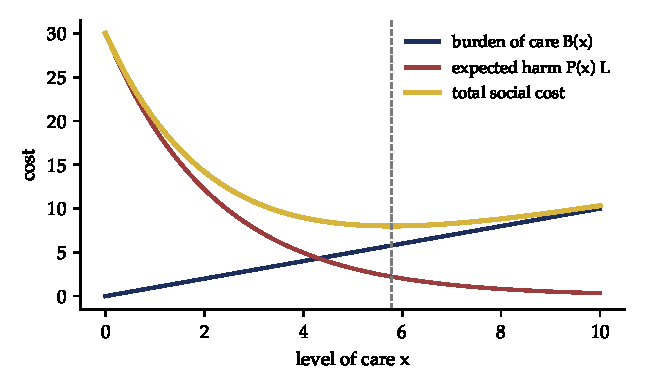
\includegraphics[width=\linewidth]{fig_hand}
\caption{The Hand formula in marginal form. The burden of care rises and the expected harm falls with the level of care. Total social cost is minimised where the slopes balance, marked by the dashed line.}
\label{fig:hand}
\end{figure}

\subsection{Where Bayes adds to Hand}

The Hand formula takes $P$ as given. Bayes asks where $P$ comes from. The reasonable person is not omniscient: the relevant probability is the one a reasonable person would have assessed using the information available, or reasonably obtainable, at the time. This has three consequences.

First, hindsight is excluded. After an accident, the probability that it would happen seems higher than it did before, because the accident has occurred. Courts warn against hindsight bias, and the Bayesian framework says precisely what is wrong with it: the accident is data that the defendant did not have, and the standard is the posterior given the defendant's information, not the information available after the accident.

Second, there is a duty to inquire. A defendant who could cheaply have obtained information that would have raised the assessed probability of harm is responsible for not obtaining it. This is a value of information calculation of the kind discussed in Chapter~\ref{ch:standards}. A manufacturer who fails to test a product, a landlord who fails to inspect wiring, an employer who ignores published research on an industrial disease, each has failed to buy information whose expected value exceeded its cost.

Third, the standard depends on the defendant's role. A professional is judged by the beliefs a reasonable member of the profession would hold. In \emph{Bolam v Friern Hospital Management Committee} the test was that a doctor is not negligent if he acted in accordance with a practice accepted as proper by a responsible body of medical opinion \citep{bolam1957}. In \emph{Bolitho} the House of Lords added that the body of opinion must be capable of withstanding logical analysis, in particular that the experts must have weighed the risks and benefits \citep{bolitho1998}. The Bayesian reading of \emph{Bolitho} is that professional practice is evidence about the reasonable posterior and the reasonable decision, but not conclusive evidence; a practice that does not reflect a coherent assessment of probabilities and utilities can be found wanting.

\section{Informed consent as expected utility}

In \emph{Montgomery v Lanarkshire Health Board} the Supreme Court held in 2015 that a doctor must take reasonable care to ensure that a patient is aware of any material risks involved in recommended treatment and of reasonable alternatives \citep{montgomery2015}. A risk is material if a reasonable person in the patient's position would be likely to attach significance to it, or if the doctor is or should be aware that this particular patient would. Nadine Montgomery, a diabetic woman of small stature, had not been told of the risk of shoulder dystocia in vaginal delivery, a risk of around nine to ten per cent for diabetic mothers, because her obstetrician judged that if told she would ask for a caesarean section.\index{Montgomery v Lanarkshire}

\emph{Montgomery} is an expected utility case. The patient, not the doctor, is the decision maker, and the patient's utilities govern. A risk is material if knowing it could change the patient's choice, which in decision terms means that the information has positive value of information for that patient. The doctor's duty is to supply information whose value to the patient exceeds the cost of supplying it, and the cost of a conversation is low. The obstetrician in \emph{Montgomery} effectively substituted her own utilities for the patient's, judging that a caesarean was worse than the patient would have judged it. The Supreme Court held that this was not her decision to make. Earlier, in \emph{Chester v Afshar}, the House of Lords had allowed recovery where a surgeon failed to warn of a small risk that then materialised, even though the patient might well have consented to the operation at a later date \citep{chester2004}. The case strains conventional causation, but it fits a view in which the patient's right to make an informed choice is itself protected.

\section{Causation}

\subsection{The but for test}

The claimant must prove that the breach caused the harm. The basic test is but for: would the harm have occurred if the defendant had not been negligent? In \emph{Barnett v Chelsea and Kensington Hospital Management Committee} a night watchman who had drunk tea laced with arsenic went to a casualty department and was sent home without examination \citep{barnett1969}. He died. The hospital was negligent, but the court found that he would probably have died even with proper treatment, because the antidote could not have been given in time. The claim failed on causation.\index{but for causation}

On the balance of probabilities the but for question becomes: is it more probable than not that the harm would not have occurred absent the breach? This is a counterfactual probability. Let $Y$ denote the harm, $Y(0)$ the harm that would have occurred without the breach and $Y(1)$ the harm with the breach. The claimant must show $\Prob(Y(0) = 0 \given Y(1) = 1, E) > 1/2$, where $E$ is the evidence. This probability is not identified by data in general, because we never observe both potential outcomes for the same person. It requires assumptions, and different assumptions give different answers. In the loss of a chance cases below, with $p_0$ the chance of a good outcome absent the breach, the all or nothing rule the courts applied is cruder than this: full recovery if $p_0 > 1/2$, nothing otherwise.

\subsection{Epidemiological evidence and the doubling of risk}

When causation must be inferred from population data, a common approach is the doubling of risk test. Suppose exposure to a substance multiplies the risk of a disease by $R$, the relative risk. Among exposed people who develop the disease, the fraction whose disease is attributable to the exposure is, under the assumption that exposure only adds cases and does not prevent or accelerate any,
\begin{equation}
\mathrm{PC} = 1 - \frac{1}{R}.
\label{eq:pc}
\end{equation}
This exceeds one half exactly when $R > 2$. Courts in England and the United States have used the test to decide whether epidemiology can establish causation on the balance of probabilities \citep{greenland1999}. Figure~\ref{fig:doubling} plots \eqref{eq:pc}.\index{doubling of risk}\index{probability of causation}

\begin{figure}[t]
\centering
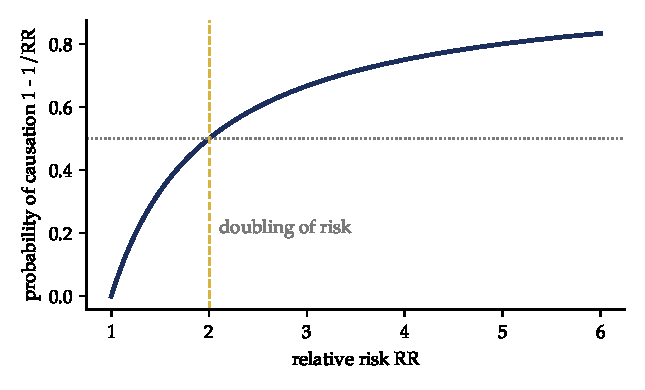
\includegraphics[width=\linewidth]{fig_doubling}
\caption{The probability of causation $1 - 1/R$ as a function of relative risk $R$. It crosses one half at $R = 2$, the doubling of risk.}
\label{fig:doubling}
\end{figure}

In \emph{Sienkiewicz v Greif} the Supreme Court considered the test in a mesothelioma case \citep{sienkiewicz2011}. Lord Phillips gave a careful account of the epidemiology, and several justices expressed doubt about deciding individual cases on statistical evidence alone. The court held that the doubling test is not a legal requirement for causation in mesothelioma cases. The Bayesian analysis explains the doubts. Equation \eqref{eq:pc} equals the probability of causation only under the assumption that exposure never prevents or accelerates disease, and is otherwise at best a lower bound (a lower bound if exposure can accelerate but never prevents disease); if exposure brings forward a disease that would have occurred later, the probability that the exposure was a cause, in the sense that the disease would not have occurred when it did, can be much larger. Greenland and Robins showed that the probability of causation is not identifiable from relative risks without further assumptions \citep{greenland1999}. The correct Bayesian response is to place a prior on the mechanism and report the posterior, recognising that the answer is assumption dependent. The court's discomfort can be read as a recognition of this dependence.

\subsection{Material contribution and Fairchild}

Mesothelioma is caused by asbestos fibres, but it is not known which fibre, or which exposure, triggers it, and a person exposed by several employers cannot prove which one caused the disease. In \emph{Fairchild v Glenhaven Funeral Services} the House of Lords held in 2002 that each employer whose negligence materially increased the risk was liable \citep{fairchild2002}. In \emph{Barker v Corus} it held that liability should be apportioned according to each employer's contribution to the risk \citep{barker2006}. Parliament promptly reversed \emph{Barker} for mesothelioma in section 3 of the Compensation Act 2006, restoring joint and several liability for the whole loss.\index{Fairchild v Glenhaven}\index{Barker v Corus}

The Bayesian analysis of \emph{Fairchild} is instructive. Suppose a worker was exposed by employers $A$, $B$, $C$ and $D$ in proportions $0.45, 0.30, 0.15, 0.10$ of total fibre dose, and suppose the risk of mesothelioma is proportional to cumulative dose. Then, given that the disease occurred, the posterior probability that it was caused by exposure from employer $j$ is proportional to that employer's dose (Figure~\ref{fig:fairchild}). No employer's probability exceeds one half, so none would be liable under the ordinary but for test, even though, if there is no background mesothelioma, it is certain that one of them caused the disease. The \emph{Fairchild} exception and the \emph{Barker} apportionment are two responses to this problem. \emph{Barker} is exactly the proportional, expected utility solution of Chapter~\ref{ch:standards}: each employer pays its expected share, and in aggregate the claimant is fully compensated if all are solvent. Section 3 of the 2006 Act chose instead to put the risk of insolvent defendants on the solvent ones.

\begin{figure}[t]
\centering
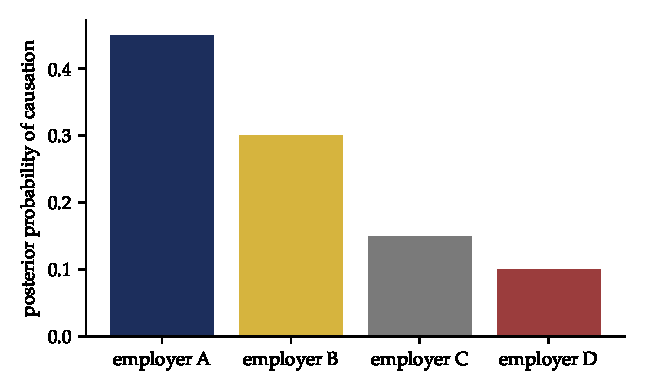
\includegraphics[width=\linewidth]{fig_fairchild}
\caption{Posterior probabilities of causation for four employers in a mesothelioma case, proportional to their shares of exposure. None exceeds one half, although their sum is one.}
\label{fig:fairchild}
\end{figure}

The earlier case of \emph{Wilsher v Essex Area Health Authority} illustrates the limits \citep{wilsher1988}. A premature baby developed retrolental fibroplasia; excess oxygen was one of five possible causes. The House of Lords refused to extend \emph{McGhee}, an earlier case about dermatitis that had allowed recovery on material increase in risk \citep{mcghee1973}, to a situation with several different possible agents. In Bayesian terms, \emph{Wilsher} involved competing causes with different mechanisms and unknown base rates, so the posterior probability that the oxygen was the cause could not be bounded away from small values. \emph{Fairchild} involved a single agent and several sources, so the probability that the agent was the cause was close to one, and only the allocation among sources was uncertain.

\section{Loss of a chance}

\subsection{Hotson and Gregg}

In \emph{Hotson v East Berkshire Area Health Authority} a boy fell from a tree and injured his hip; the hospital negligently failed to diagnose the injury for five days; he developed avascular necrosis \citep{hotson1987}. The trial judge found that even with prompt treatment there was a seventy five per cent chance he would have developed the condition, and awarded a quarter of the damages for the lost twenty five per cent chance. The House of Lords reversed: on the balance of probabilities the fall, not the delay, caused the necrosis, so the claim failed entirely.\index{loss of chance}\index{Hotson v East Berkshire}

In \emph{Gregg v Scott} a doctor negligently failed to refer a patient with a lump that turned out to be non Hodgkin lymphoma \citep{gregg2005}. The delay reduced his estimated chance of being cured, defined as surviving ten years disease free, from forty two per cent to twenty five per cent. A majority of the House of Lords held that he could not recover for the loss of a chance in a clinical negligence case. Since his chance of cure had never exceeded one half, it could not be shown that the negligence more probably than not caused the loss of a cure.\index{Gregg v Scott}

\subsection{The Bayesian analysis}

The majority in \emph{Gregg} treated the patient's outcome as determined, so that the question was whether he was one of the patients who would have been cured with prompt treatment. Lord Hoffmann put this sharply: the law regards the world as a deterministic place, and the question is what happened, not what the chances were. On that view, the forty two per cent was not a property of the patient but a statement of ignorance about which group he belonged to, and the claimant had to prove on the balance of probabilities that he was in the group who would have been cured and were not because of the delay.

The minority, Lord Nicholls and Lord Hope, held that the patient lost something of value, a chance of cure, and that he should be compensated for it. Lord Nicholls said that it would be irrational and indefensible for the law to recognise a forty five per cent chance as worth nothing when a fifty five per cent chance is worth the whole.

The Bayesian view is that the forty two per cent is the posterior probability of cure under prompt treatment, given everything known about the patient. Whether the world is deterministic is beside the point: the court must act on its probabilities, not on the unknown truth. The question is which remedy minimises expected loss across cases like this one. The all or nothing rule overcompensates claimants just above one half and undercompensates those below it. The proportional rule compensates each claimant by his expected loss and, aggregated across cases, compensates the class exactly. It also gives the right incentives to doctors: under the all or nothing rule a doctor whose negligence reduces patients' chances from forty to twenty per cent faces no liability at all, while one whose negligence reduces them from sixty to forty faces full liability. That is not a rational incentive structure. Our paper argues that the majority's reasoning in \emph{Gregg} rests on a mistaken view of what probability measures, and that proportional recovery is the coherent rule \citep{polson_sokolov_tort}.\index{proportional liability}

English law already accepts proportional recovery for lost chances in other settings. In \emph{Allied Maples v Simmons and Simmons} the claimant lost the chance of negotiating protection in a contract because of its solicitors' negligence \citep{alliedmaples1995}. The Court of Appeal held that where the outcome depended on the hypothetical action of a third party, the claimant need only show a substantial chance, and damages would be discounted by the probability. The distinction between clinical cases and cases depending on a third party's choice has never been convincingly explained. In French law, as Chapter~\ref{ch:commoncivil} discusses, \emph{perte de chance} is recognised in medical cases, and damages are proportional to the lost chance. The comparison is a good example of how two legal systems can reach different answers to a question that has a clear Bayesian solution.

\section{Remoteness and foreseeability}

In \emph{The Wagon Mound (No 1)} the Privy Council held that a defendant is liable only for damage of a kind that was reasonably foreseeable \citep{wagonmound1961}. Oil spilled from a ship in Sydney Harbour drifted to a wharf where welding was taking place, caught fire and damaged the wharf. The court found that fire was not a foreseeable consequence of the spill, because experts believed furnace oil on water could not be ignited. In \emph{The Wagon Mound (No 2)}, a different claimant on the same facts, with different evidence, the court found that a reasonable ship's engineer would have recognised a small but real risk of fire, and that since the risk could have been eliminated at no cost, the defendant was liable \citep{wagonmound1967}.\index{Wagon Mound}

The two cases differ in the evidence about the probability of fire and show that foreseeability is a probability judgment made on the evidence before the court. \emph{Wagon Mound (No 2)} also shows the Hand formula at work: a small probability suffices for liability when the precaution is costless. Lord Reid, reinterpreting \emph{Bolton v Stone}, distinguished it from the oil spill: there the risk was small and the precaution costly, here the risk was small and the precaution free. This balance of risk against cost is his gloss in \emph{Wagon Mound (No 2)}; the speech in \emph{Bolton} itself did not weigh cost.

\section{Duty of care}

The duty of care is the most normative element of negligence, and the one least amenable to a probabilistic reading. In \emph{Donoghue v Stevenson} Lord Atkin's neighbour principle said that one must take reasonable care to avoid acts or omissions which one can reasonably foresee would be likely to injure one's neighbour \citep{donoghue1932}. Foreseeability is again probability. In \emph{Caparo Industries v Dickman} the House of Lords added the requirements of proximity and that it be fair, just and reasonable to impose a duty \citep{caparo1990}. In \emph{Robinson v Chief Constable of West Yorkshire} the Supreme Court emphasised incremental development by analogy with established categories \citep{robinson2018}.\index{duty of care}\index{Caparo v Dickman}

Proximity and fairness are policy judgments, but they can be framed as judgments about incentives and about the allocation of losses, which brings them within decision theory. A duty that would expose auditors to indeterminate liability to anyone who reads their reports, the concern in \emph{Caparo}, would raise the cost of audits and might reduce their supply without improving their quality. The question is whether imposing the duty improves expected social welfare, a question that requires evidence about behaviour, not a fixed formula. Chapter~\ref{ch:misrep} develops this for the case of statements and advice.

\section{Contributory negligence and apportionment}

Under the Law Reform (Contributory Negligence) Act 1945, where a claimant suffers damage partly through his own fault, damages are reduced to the extent the court thinks just and equitable having regard to the claimant's share in the responsibility. Courts in practice apportion by a combination of causal potency and blameworthiness. A decision theoretic analysis suggests that apportionment should be chosen to give both parties efficient incentives, by reference to the incentives each party faces. In the standard bilateral care model of Shavell, however, negligence with a defence of contributory negligence, or comparative negligence, with due care standards set efficiently induces efficient care whatever the division of the loss \citep{shavell1987}. Apportionment therefore matters for incentives chiefly when the courts are uncertain about the standard, make errors, or when activity levels matter.

\section{Strict liability}

Some torts do not require negligence. Under \emph{Rylands v Fletcher}, a person who brings onto his land something likely to do mischief if it escapes is answerable for the damage it causes \citep{rylands1868}. Strict liability shifts the whole expected cost of an activity to the actor, who then chooses both the level of care and the level of activity efficiently (in the unilateral case; in the bilateral model, strict liability without a contributory negligence defence leaves the victim no incentive to take care). Negligence liability induces efficient care but not efficient activity levels, because the actor who takes due care escapes liability for the residual risk. Shavell's analysis of this distinction is a classic of law and economics \citep{shavell1987}. The Bayesian contribution is again about information: strict liability is attractive when the actor knows more than the court about the probability of harm, because it puts the decision in the hands of the party with the better posterior.

\section{Summary}

Negligence is a failure of epistemic or decision responsibility. Breach is a failure to minimise expected cost given reasonable beliefs; foreseeability and remoteness are probability judgments; causation is a counterfactual probability that requires modelling assumptions; and loss of a chance is a case where the all or nothing rule conflicts with the logic of expected loss. English tort law is more Bayesian than its judges usually admit, and where it departs from Bayesian reasoning, as in \emph{Gregg v Scott}, the departure is costly. Chapter~\ref{ch:misrep} applies the same framework to misrepresentation, where the defendant's beliefs, and what he said about them, are the subject of the claim.

\section*{Notes and Questions}
\addcontentsline{toc}{section}{Notes and Questions}
\begin{enumerate}[label=\arabic*.]
\item In \emph{Bolton v Stone}, suppose six balls left the ground in thirty seasons and that a ball leaving the ground strikes a person with probability $0.02$. With a gamma prior of shape one and rate one on the annual rate (Appendix~\ref{app:toolkit}), compute the posterior expected annual probability of injury. If an injury costs one hundred thousand pounds and a fence would cost fifty thousand pounds and last twenty years, was the club negligent on the Hand formula?
\item Show that if exposure can accelerate disease onset, the probability of causation can exceed $1 - 1/R$. Construct an example.
\item In the \emph{Fairchild} example, suppose employer $A$ is insolvent. Compare the claimant's recovery under \emph{Barker} apportionment and under section 3 of the Compensation Act 2006.
\item Under all or nothing and proportional rules, compute the expected liability of a doctor whose negligence reduces patients' chances of cure from $p_0$ to $p_1$, as functions of $p_0$ and $p_1$. Which rule gives incentives proportional to the harm done?
\item Write a short judgment in \emph{Gregg v Scott} adopting the Bayesian analysis. Address Lord Hoffmann's argument that the world is deterministic.
\item Explain why \emph{Montgomery} can be described as a value of information test.
\end{enumerate}

\section*{Further reading}
Our paper sets out the program of this chapter in more detail \citep{polson_sokolov_tort}. Shavell's \emph{Economic Analysis of Accident Law} remains the best economic treatment \citep{shavell1987}. On probability of causation, Greenland and Robins \citep{greenland1999}. Lord Phillips's speech in \emph{Sienkiewicz} is a rare judicial engagement with epidemiology \citep{sienkiewicz2011}.

\chapter{Mass Torts and Scientific Causation}
\label{ch:masstorts}

\section{Many claimants, one question}

A mass tort is a set of claims arising from a common cause: a drug, a medical device, a chemical, a consumer product. Thousands or hundreds of thousands of claimants allege that exposure caused their illness. The defendants deny that the product causes the illness at all, or that it caused it in particular claimants. The litigation turns on science: epidemiology, toxicology, pharmacology, and the interpretation of studies that often disagree. Courts must decide scientific questions under uncertainty, with enormous sums at stake and with experts on each side who read the same studies differently.\index{mass torts}

Mass torts raise two causal questions. General causation asks whether the product can cause the illness: does exposure raise the risk in the population? Specific causation asks whether it caused this claimant's illness. The first is a question about a population parameter, the relative risk, and is answered by epidemiology. The second is a question about an individual, answered, if at all, by combining the population evidence with facts about the claimant. Chapter~\ref{ch:tort} discussed the probability of causation and the doubling of risk. This chapter treats general causation as a problem of Bayesian evidence synthesis, examines how courts have managed scientific evidence in mass torts, and draws lessons from several major episodes.

\section{General causation as evidence synthesis}

\subsection{The evidence}

The evidence for general causation is a body of studies: randomised trials where they exist, cohort and case control studies, animal experiments and mechanistic research. Each study estimates a relative risk with uncertainty, and the estimates differ because of sampling error, differences in populations and exposures, and biases in design. The question for a court is what the body of evidence, taken together, says about the true relative risk.\index{general causation}

\subsection{Hierarchical meta analysis}

A Bayesian random effects meta analysis models each study's estimate $y_j$, on the log relative risk scale, as
\begin{equation}
y_j \sim N(\theta_j, s_j^2), \qquad \theta_j \sim N(\mu, \tau^2),
\label{eq:meta}
\end{equation}
where $s_j$ is the study's standard error (the uncertainty from sampling alone), $\theta_j$ its true effect, $\mu$ the average effect across studies, and $\tau^2$ the between study variance (how much true effects differ from one study to the next). The random effects in the name are the $\theta_j$, which vary across studies around $\mu$. Priors on $\mu$ and $\tau$ complete the model. The posterior for $\mu$ answers the general causation question: what is the probability that the typical relative risk, $e^{\mu}$, exceeds one (general causation) or two (the doubling threshold relevant to specific causation)? The posterior for $\tau$ says how much the effect varies across settings. Bias can be modelled explicitly, for instance by allowing observational studies a bias term with a prior reflecting how much confounding is plausible.\index{meta analysis}

This approach has two advantages over the way experts often present evidence in court. First, it combines all the studies coherently and makes any selection explicit, rather than leaving it hidden in favourable choices, which is the adversarial expert problem that Chapter~\ref{ch:fienberg} examines. Second, it reports a probability that the effect is real and of a given size, which is what a court needs, rather than a collection of p values.

\subsection{The Bradford Hill considerations}

Epidemiologists and courts often refer to the considerations set out by Austin Bradford Hill in 1965 for judging whether an association is causal: strength, consistency, specificity, temporality, biological gradient, plausibility, coherence, experiment and analogy \citep{hill1965}. Hill did not intend them as a checklist, and courts that apply them mechanically miss their point. Each consideration is a reason to update beliefs about causation. A strong association is harder to explain by confounding; a consistent association across settings makes chance and setting specific bias less likely; a dose response gradient is predicted by causation and less so by most biases; biological plausibility raises the prior. A Bayesian treatment turns the considerations into components of the likelihood and the prior, which can be combined rather than counted.\index{Bradford Hill}

\section{Daubert and the gatekeeper}

The Supreme Court's decision in \emph{Daubert} \citep{daubert1993}, discussed in Chapter~\ref{ch:evidence}, arose from mass tort litigation over Bendectin, a drug for morning sickness alleged to cause birth defects. By the early 1990s, many epidemiological studies had found no association, and the plaintiffs' experts relied on animal studies, chemical structure analysis and reanalyses of the published studies. The Court held that trial judges must assess the reliability of expert evidence, and on remand the Ninth Circuit excluded the plaintiffs' experts. In \emph{General Electric v Joiner} the Court held that a trial judge may exclude an expert whose conclusions do not follow from the studies on which he relies, because there is too great an analytical gap between the data and the opinion \citep{joiner1997}.\index{Daubert}\index{General Electric v Joiner}

The gatekeeping role asks judges to evaluate scientific reasoning, which most are not trained to do. The analytical gap of \emph{Joiner} is, in Bayesian terms, a gap between the likelihood the studies supply and the posterior the expert claims. An expert who infers a large relative risk from studies that, combined, are consistent with no effect has made an inference the evidence does not support. A judge equipped with a meta analytic posterior can see the gap directly.

\section{Court appointed experts}

In the breast implant litigation of the 1990s, hundreds of thousands of women claimed that silicone implants caused connective tissue and autoimmune diseases. Juries returned large verdicts, and the leading manufacturer filed for bankruptcy. Several courts appointed independent experts. In \emph{Hall v Baxter Healthcare}, Judge Robert Jones in Oregon appointed four technical advisors, in epidemiology, rheumatology, immunology and toxicology, and polymer chemistry, and after hearing them excluded the plaintiffs' expert evidence of causation \citep{hall1996}. A national panel appointed in the federal multidistrict litigation reported in 1998 that the evidence did not show an association between implants and the diseases alleged \citep{nationalsciencepanel1998}, and the Institute of Medicine concluded in 1999 that the evidence did not show that implants cause these diseases \citep{iom1999}.\index{breast implants}\index{court appointed experts}

The breast implant experience supports the recommendation of Fienberg's panel, which Chapter~\ref{ch:fienberg} discusses, that courts make more use of neutral experts. A neutral panel provides a draw from the unselected distribution of expert opinion, and in a mass tort, where the same scientific question arises in thousands of cases, its findings can be applied across them. One Bayesian view is that a neutral panel's synthesis is the court's best estimate of the posterior on general causation, to be updated by any new studies, rather than relitigated in every trial, although binding non-parties to a finding raises due process limits.

\section{Specific causation}

\subsection{From population to individual}

Once general causation is established, each claimant must show that the product caused her illness. If the relative risk is $R$ and nothing distinguishes the claimant from the exposed population in the studies, the probability of causation is $1 - 1/R$ under the assumptions of equation~\eqref{eq:pc} in Chapter~\ref{ch:tort}, and at least that if exposure can also accelerate onset. Individual facts can move this probability: a higher dose than average, a latency consistent with the known induction period, the absence of other risk factors, or a biomarker associated with the exposure raises it; a family history or another known cause lowers it. A Bayesian treatment updates the population probability of causation with the claimant's individual evidence, using likelihood ratios for each factor.\index{specific causation}

\subsection{Differential etiology}

Experts often address specific causation by differential etiology: listing possible causes of the claimant's illness and ruling them out until one remains. The method is legitimate only if the list is complete and the ruling out is evidence based. Many illnesses have no identifiable cause in most patients; ruling out known alternatives does not establish that the product was the cause if most cases are idiopathic. The Bayesian version makes this explicit: the posterior probability that the product was the cause is its prior weight times its likelihood, divided by the sum over all causes including unknown ones. If the unknown cause has a large prior weight, eliminating the other known causes leaves the product's probability well below one. This is the island formula, equation~\eqref{eq:islandsimple} of Chapter~\ref{ch:classic}, applied to causes rather than suspects.

\section{Episodes}

\subsection{Agent Orange}

Veterans of the Vietnam War sued the manufacturers of Agent Orange, a herbicide contaminated with dioxin, alleging that exposure caused cancers in themselves and birth defects in their children. Judge Jack Weinstein, whom we met in Chapter~\ref{ch:standards} and will meet again in Chapter~\ref{ch:kadane}, presided over the class action. In 1984 the parties settled for one hundred and eighty million dollars, reportedly the largest product liability class settlement up to that time. Weinstein later dismissed the claims of veterans who opted out, finding that the epidemiological evidence did not establish causation for the diseases claimed. Weinstein was explicit that he was making a probabilistic judgment about a population, and he favoured approaches that would compensate claimants in proportion to the probability of causation rather than all or nothing, the expected utility approach of Chapter~\ref{ch:standards}.

\subsection{Vioxx}

Vioxx, an anti inflammatory drug, was withdrawn from the market in 2004 after a randomised trial showed an increased risk of heart attacks and strokes. Unlike many mass torts, the evidence for general causation came from randomised trials, and the debate concerned the size of the risk, its dependence on duration of use, and when the manufacturer knew. The litigation settled in 2007 for about four point eight five billion dollars, under a programme that paid claimants according to criteria related to the strength of their individual evidence: duration of use, timing of the event and other risk factors. The settlement grid was, to a first approximation, a schedule of probabilities of causation applied to individuals, although the points also reflected injury severity and litigation risk.

\subsection{Glyphosate}

In 2015 the International Agency for Research on Cancer classified glyphosate, the active ingredient in the herbicide Roundup, as probably carcinogenic to humans, based on limited human evidence of an association with non Hodgkin lymphoma, sufficient evidence in experimental animals, and strong mechanistic evidence. The United States Environmental Protection Agency and the European Food Safety Authority concluded that glyphosate was not likely to be carcinogenic at realistic exposures. Juries in several trials returned large verdicts for plaintiffs, and in 2020 Bayer, which had acquired Monsanto, agreed to a settlement programme of up to about eleven billion dollars, with litigation continuing. The glyphosate episode shows how different bodies, applying different standards to the same evidence, can reach different conclusions. The IARC classification is a hazard assessment, asking whether a substance can cause cancer under some conditions; regulatory risk assessment asks whether it does at actual exposure levels; a jury asks whether it more probably than not caused a particular plaintiff's cancer. Each is a different question, with a different threshold, and conflating them is a source of confusion.

\section{Aggregation and its limits}

Mass torts strain the individual adjudication model of the common law. Trying hundreds of thousands of claims individually is impossible; class actions and multidistrict litigation aggregate them, and bellwether trials of selected cases inform global settlements. Statistically, bellwether trials are a sample used to estimate the value of the remaining claims, and their usefulness depends on how they are selected. If each side picks its strongest cases, the outcomes are biased in both directions, as with selected experts. Random selection of bellwether cases, which some judges have ordered, yields an unbiased sample, although randomly selected cases are often dismissed or settled before trial, so the tried cases may no longer be random, and allows the results to be extrapolated with stated uncertainty.

Aggregate approaches raise fairness questions. A claimant whose individual case is strong may receive less in a global settlement than she would at trial; one whose case is weak may receive more. A settlement grid that pays according to probability of causation is the Bayesian compromise: each claimant receives the expected harm the product caused her, given the evidence, without the cost of individual trial. This is the logic of proportional liability extended to an entire litigation.

\section*{Notes and Questions}
\addcontentsline{toc}{section}{Notes and Questions}
\begin{enumerate}[label=\arabic*.]
\item Five studies report log relative risks of $0.4, 0.1, 0.6, -0.1, 0.3$ with standard errors of $0.2, 0.15, 0.3, 0.25, 0.2$. Fit the model \eqref{eq:meta} with a flat (uniform, uninformative) prior on $\mu$ and $\tau$ fixed at $0.1$. What is the posterior probability that the typical relative risk, $e^{\mu}$, exceeds one (general causation), and that it exceeds two (the doubling threshold)? Contrast the two answers.
\item Explain how each Bradford Hill consideration would enter a Bayesian analysis as a likelihood or a prior.
\item A claimant was exposed to the product. Among exposed people with her illness, the product accounts for twenty per cent of cases, two other known causes for twenty per cent between them, and an unknown cause for the remaining sixty per cent. Experts rule out the two other known causes. What is the posterior probability that the product caused her illness?
\item Design a protocol for selecting bellwether cases in a mass tort. What statistical properties should it have?
\item Compare the questions answered by a hazard classification, a regulatory risk assessment and a jury verdict in the glyphosate litigation. Which threshold applies to each?
\item Should courts compensate mass tort claimants in proportion to the probability of causation? Consider incentives for manufacturers, fairness to claimants, and administrative cost.
\end{enumerate}

\section*{Further reading}
Hill's 1965 address \citep{hill1965}; the Federal Judicial Center's \emph{Reference Manual on Scientific Evidence}, especially its chapters on epidemiology and statistics \citep{fjc2011}; Greenland and Robins on the probability of causation \citep{greenland1999}.

\chapter{Assessing Damages Under Uncertainty}
\label{ch:damages}

\section{A number from a distribution}

Once liability is established, a court must put a number on the loss. The number is rarely known. A claimant injured at thirty will lose earnings over a working life whose length, wages and health are uncertain. A business whose contract was broken lost profits it might or might not have made. An investor misled into buying shares lost the difference between what she paid and what the shares would have been worth, a counterfactual price. In each case the court must turn a distribution of possible losses into a single award, usually a lump sum paid once and never revised. This chapter treats the assessment of damages as a Bayesian decision problem: form the posterior distribution of the loss, choose a loss function that reflects the law's objectives, and choose the award that minimises expected loss.\index{damages}

\section{The compensatory principle}

The basic principle in English and American law is that damages should put the claimant in the position she would have been in had the wrong not occurred, so far as money can. In contract, that is the position had the contract been performed; in tort, the position had the tort not been committed. Both are counterfactuals. Let $\theta$ be the claimant's loss, the difference in value between the counterfactual position and her actual position. The principle says the award should equal $\theta$. Since $\theta$ is uncertain, the court must estimate it.\index{compensatory principle}

\subsection{Which estimate?}

Decision theory says the right estimate depends on the loss function. If over compensation and under compensation by the same amount are equally bad, and badness grows with the square of the error, the optimal award is the posterior mean of $\theta$. If badness grows linearly, it is the posterior median. If under compensation is $k$ times as bad as over compensation, with linear loss, it is the posterior quantile at $k/(1+k)$. Each choice is defensible; the law rarely says which it is making.

The posterior mean has a special property: across many cases, awards equal to the mean compensate claimants as a class exactly on average, and defendants as a class pay, on average, the harm they caused. This aggregate accuracy matters for incentives, since defendants' expected liability then equals the expected harm, the condition for efficient care to which Chapter~\ref{ch:becker} returns, provided that every harm leads to a claim. For this reason we think the posterior mean is the default the law should adopt.

\section{Future losses}

\subsection{Lump sums and discounting}

Damages for future losses, such as lost earnings or the cost of care, are usually paid as a lump sum. The sum must be enough, invested, to provide the lost income over the relevant period. Two uncertain quantities determine it: the stream of future losses and the return on investment. English courts compute the lump sum using a multiplier\index{multiplier}, derived from actuarial tables known as the Ogden tables, applied to an annual loss, the multiplicand. The multiplier depends on the claimant's life expectancy or working life and on the discount rate, which is set by the Lord Chancellor under the Damages Act 1996. In \emph{Wells v Wells} the House of Lords held that the discount rate should reflect the return on index linked government stock, since claimants should not be required to take investment risk \citep{wells1999}. The rate has been changed several times since, including to a negative value in 2017, reflecting low real yields. The Civil Liability Act 2018 then departed from \emph{Wells}: the rate is now set on the assumption that the claimant invests in a low risk diversified portfolio, and on that basis it was set at minus one quarter of one per cent in 2019 and at plus one half of one per cent in 2025.\index{discount rate}\index{Ogden tables}

The discount rate matters a great deal. For a claimant with forty years of future loss, the multiplier for a fixed term of forty years, ignoring mortality, at a real rate of minus one quarter of one per cent is about forty two; at plus one half of one per cent it is about thirty six; at two and a half per cent it is about twenty five. A change in the rate of under three percentage points changes the award by more than a third. Setting the rate is a choice about who bears investment risk: a low rate protects claimants from poor returns, at a cost to defendants and their insurers.

\subsection{The predictive distribution}

A Bayesian assessment of future loss forms the predictive distribution of the present value of the loss, combining uncertainty about working life, wages and returns. Figure~\ref{fig:damages} shows a simulated example: a claimant with an expected remaining working life of twenty two years, with uncertainty, and an annual wage with uncertainty about its level, discounted at half of one per cent. The distribution is skewed: its mean exceeds its median, because high wages produce large losses. An award at the median would under compensate on average; an award at the mean would compensate the class exactly on average.

\begin{figure}[t]
\centering
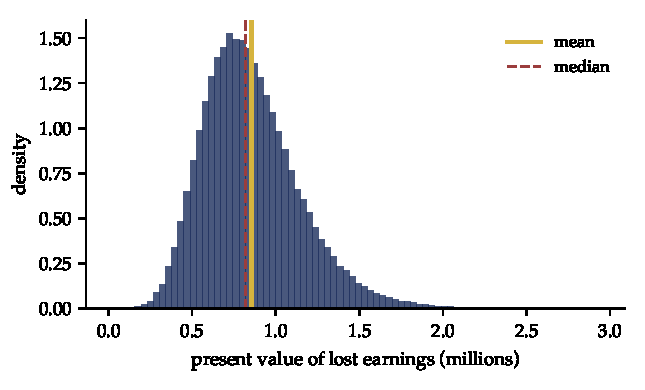
\includegraphics[width=\linewidth]{fig_damages}
\caption{Simulated predictive distribution of the present value of lost earnings, with uncertainty about working life and wages. The mean exceeds the median because the distribution is skewed to the right.}
\label{fig:damages}
\end{figure}

\subsection{Contingencies}

English courts adjust multipliers for contingencies other than mortality, such as unemployment, ill health and early retirement, using discounts in the Ogden tables that depend on the claimant's employment status, education and disability. These adjustments are expected value calculations: they reduce the award by the expected effect of events that would have reduced earnings in any case. Their basis is population data, and they can be individualised where the evidence supports it, by Bayesian updating of the population rates with evidence about the claimant.

\subsection{Periodical payments}

The Damages Act 1996, as amended by the Courts Act 2003, allows courts to order periodical payments\index{periodical payments} instead of a lump sum for future pecuniary loss, and requires them to consider whether such an order would be appropriate. Periodical payments, linked by default to the Retail Prices Index (earnings indexation, now usual for care costs, is available by a court order modifying the default, as in \emph{Thompstone v Tameside and Glossop Acute Services NHS Trust} \citep{thompstone2008}), transfer longevity and investment risk from the claimant to the defendant, who is usually an insurer or the National Health Service. In decision terms, they replace a point estimate of an uncertain quantity with a contract that pays the realised value. They remove the claimant's longevity risk, and they are used for the largest claims, such as those for catastrophic injury, where the uncertainty is greatest.

\section{Lost profits and the reasonable certainty rule}

\subsection{The rule}

American courts traditionally require that lost profits be proved with reasonable certainty, and have been reluctant to award profits for new businesses with no track record. In \emph{Story Parchment Co v Paterson Parchment Paper Co} the Supreme Court held in 1931 that where the fact of damage is certain, uncertainty about its amount does not bar recovery, and that the wrongdoer who created the uncertainty should bear its risk \citep{storyparchment1931}. English law follows similar principles: once loss is proved, the court must do its best to quantify it, and the difficulty of quantification is not a reason to award nothing.\index{lost profits}

\subsection{The Bayesian view}

The reasonable certainty rule conflates two questions. The first is whether there was a loss at all, a question of liability. The second is how large it was, a question of quantification. A Bayesian treats both as uncertain and integrates. If the probability that the business would have been profitable is $q$ and its expected profit if profitable is $\mu$, the expected loss is $q\mu$. A rule that awards nothing unless $q$ is high and awards $\mu$ if it is, is an all or nothing rule with the defects discussed in Chapter~\ref{ch:standards}. The proportional award $q\mu$ is the expected loss, and it gives the defendant the right incentives.

\subsection{Loss of a chance in contract}

English contract law has long accepted this logic. In \emph{Chaplin v Hicks} a theatre manager in breach of contract prevented the claimant from attending an interview in a beauty contest in which she was one of fifty finalists for twelve prizes; the Court of Appeal upheld an award for the loss of her chance, although it could not be known whether she would have won \citep{chaplin1911}. \emph{Allied Maples}, discussed in Chapter~\ref{ch:tort}, extended the principle to the hypothetical actions of third parties. Damages for a lost chance are the probability of success times the value of success, an expected value, discounted for any other contingencies.

\section{Damages against the wrongdoer}

\subsection{Evidential presumptions}

Where the defendant's wrong has made it impossible to measure the loss, courts often resolve uncertainty against the defendant. In \emph{Armory v Delamirie}, decided in 1722, a chimney sweep's boy found a jewel and took it to a goldsmith, whose apprentice removed the stones; the court directed the jury to presume the stones were of the finest water and assess damages accordingly, unless the goldsmith produced them \citep{armory1722}. The presumption is a rule about which posterior quantile to use: when the defendant has destroyed the evidence, the court uses a high quantile, shifting the cost of uncertainty to the party responsible for it.

In decision theoretic terms, the presumption serves an ex ante objective. If uncertainty were resolved at the posterior mean, a wrongdoer could profit from destroying evidence whenever the evidence would have shown a loss above the mean. Resolving uncertainty against the wrongdoer removes that incentive. The same logic underlies the adverse inference from a party's failure to call evidence it controls, and the rules on spoliation.

\subsection{Negotiating damages}

Where a defendant breaches a restrictive covenant over land or uses another's property without permission, courts may award damages measured by the sum the parties would reasonably have agreed for the release of the obligation. In \emph{Morris-Garner v One Step (Support) Ltd} the Supreme Court explained these negotiating damages\index{negotiating damages} as a measure of the value of the right lost, appropriate where that right was an asset with economic value \citep{morrisgarner2018}; the Court held that difficulty in proving financial loss is not by itself a reason to award them, and refused them on the facts, where the breach of non-compete covenants had caused ordinary financial loss. The hypothetical negotiation is a counterfactual bargaining problem: the court asks what two reasonable parties, with the information then available, would have agreed. A Bayesian treatment models each party's valuation and the bargaining outcome, such as the midpoint of the zone of agreement, using the information available at the date of the hypothetical negotiation.

\section{Hindsight in damages}

Should the assessment of damages use information that became available after the wrong? In \emph{Golden Strait Corporation v Nippon Yusen Kubishika Kaisha (The Golden Victory)} a charterer repudiated a charter with nearly four years to run, and the Second Gulf War, which would have entitled the charterer to cancel, broke out fifteen months later; the House of Lords held, by a majority, that damages should take account of the war, since the compensatory principle requires that the claimant receive no more than it would have received had the contract been performed \citep{goldenvictory2007}. The minority emphasised commercial certainty and the date of breach rule.

Chapter~\ref{ch:bankruptcy} returns to the same question in a different setting, the solvency of a firm judged after its failure. The Bayesian answer distinguishes the information set relevant to liability, which is fixed at the time of the act, from the information relevant to quantum, which can include later events because the loss itself unfolds over time. The posterior for the loss should condition on everything known at the date of assessment about events that would have affected the counterfactual position. \emph{The Golden Victory} is consistent with that principle; the minority's concern for certainty is a concern about the cost of uncertainty in commercial transactions, which is a legitimate input to the choice of rule.

\section{Experts and the combination of estimates}

Damages in commercial cases are often the subject of competing expert reports, using different models: discounted cash flows, comparable transactions, market prices. As Chapter~\ref{ch:fienberg} explains, experts are selected for favourable results, and the court sees two tails of the distribution of possible opinions. A Bayesian court treats each report as a signal, assesses its reliability, and combines them, rather than choosing one or splitting the difference. Where the experts agree on most inputs and disagree on a few, the court should focus on the disputed inputs and form its own posterior for each, then compute the damages implied. Judges do this informally when they accept one expert's discount rate and another's growth assumptions. Making the process explicit, with a table of inputs, the evidence for each and the resulting posterior, makes the judgment transparent and appealable on its merits.

\section{Interest and the time value of money}

A claimant compensated years after the loss has also lost the use of the money. Statutory and equitable interest compensate for this, at rates set by statute or by the court. The appropriate rate is a question about the claimant's counterfactual investment or borrowing, which is uncertain. In \emph{Sempra Metals v Inland Revenue Commissioners} the House of Lords allowed compound interest as restitutionary interest on tax paid under a mistake \citep{sempra2007}, though the Supreme Court has since held that no claim in unjust enrichment lies for compound interest on mistaken payments, so that this holding was overruled \citep{prudential2018}. Compound interest is the correct measure of the time value of money; simple interest systematically under compensates long delayed claims, a point of direct relevance to slow court systems such as those of Chapter~\ref{ch:india}.

\section{Damages in the age of data}

Data now inform damages more than ever. Earnings losses can be estimated from large panels of workers with similar characteristics; the costs of care from records of actual expenditure; the value of lost businesses from market data. Machine learning models can predict individual trajectories with uncertainty. These methods support the Bayesian approach of this chapter: they produce predictive distributions rather than point estimates, and they can be individualised by conditioning on the claimant's characteristics. The legal questions are which loss function to apply, whether to use the mean or another summary, and how to handle the risk that remains, by periodical payments, by insurance, or by accepting it.

\section*{Notes and Questions}
\addcontentsline{toc}{section}{Notes and Questions}
\begin{enumerate}[label=\arabic*.]
\item Compute the multiplier for forty years of annual loss at real discount rates of minus one quarter, plus one half and plus two and a half per cent. By what percentage does the award fall between the first and last?
\item A claimant's working life is uncertain, with mean twenty years and standard deviation five. Show by simulation that the expected present value is less than the present value at the expected working life when the discount rate is positive, and greater when it is negative. Why?
\item A start up's chance of becoming profitable was forty per cent, and its expected profits if profitable were five million. Under the reasonable certainty rule, what would a court likely award? Under the expected value approach?
\item In \emph{Chaplin v Hicks}, the claimant was one of fifty finalists for twelve prizes. What was her chance of a prize? How should the court value it?
\item Explain the presumption in \emph{Armory v Delamirie} as a choice of posterior quantile. What incentive does it create?
\item Should \emph{The Golden Victory} be followed in a market where contracts are routinely traded? Frame your answer in terms of the cost of uncertainty.
\end{enumerate}

\section*{Further reading}
\emph{Wells v Wells} on discounting \citep{wells1999}; \emph{Story Parchment} on uncertain damages \citep{storyparchment1931}; \emph{Morris-Garner} on negotiating damages \citep{morrisgarner2018}; \emph{The Golden Victory} on hindsight \citep{goldenvictory2007}; \emph{Chaplin v Hicks} on loss of a chance \citep{chaplin1911}; \emph{Armory v Delamirie} on evidential presumptions \citep{armory1722}; \emph{Sempra Metals} on interest \citep{sempra2007}.

\chapter{Misrepresentation as a Bayesian Constraint}
\label{ch:misrep}

\section{Statements as signals}

Much of commercial life consists of people telling other people what they believe. A seller describes a property, an auditor certifies accounts, a broker presents a risk to an insurer, a fund manager reports the assets in a fund. Each statement is a signal, and the recipient uses it to update beliefs and then to act: to buy, to lend, to insure, to invest. The law of misrepresentation governs these signals. It asks when a false statement gives the recipient a remedy, and what remedy.\index{misrepresentation}

In our tort paper we argued that the doctrines of misrepresentation are best understood as constraints on the relationship between what a speaker says and what the speaker's evidence warrants \citep{polson_sokolov_tort}. A statement of fact implicitly asserts that the speaker's posterior probability for the fact is high. Fraud is the assertion of a high probability when the speaker's actual posterior is low, or when the speaker has no posterior at all because he has not looked. Negligent misstatement is the assertion of a probability that the speaker's evidence does not warrant, because the speaker has failed to reason as a competent person in his position would. Innocent misrepresentation is the assertion of a probability that was warranted by the speaker's evidence, although the fact asserted turned out to be false. The remedies differ accordingly. This chapter develops the framework and applies it to the main English authorities and to insurance law, and closes with Bayesian persuasion and proper scoring rules as limits on what a statement may convey.

\section{A model of assertion}

Let $\theta$ be a fact about which the speaker makes a statement, and let $D_S$ be the speaker's information. A competent speaker in the speaker's position, reasoning correctly from $D_S$, would hold posterior $p_S = \Prob(\theta \given D_S)$. The speaker's actual belief, which may differ from $p_S$ because the speaker has reasoned badly or not at all, is $b_S$. The speaker makes a statement $s$, and a reasonable recipient interprets $s$ as conveying a probability $q(s)$ for $\theta$. For a flat assertion that $\theta$ is true, $q(s)$ is close to one; for an expression of opinion, such as the speaker believes $\theta$, it may be lower; for a statement hedged with qualifications, lower still.\index{assertion, model of}

The recipient's information is $D_R$, and after hearing $s$ the recipient's posterior becomes
\begin{equation}
\Prob(\theta\given D_R, s) \propto \Prob(s \given \theta, D_R)\,\Prob(\theta\given D_R).
\end{equation}
If the recipient trusts the speaker completely, $\Prob(\theta\given D_R,s) = q(s)$. More generally, the recipient's update depends on the likelihood ratio $\Prob(s\given\theta,D_R)/\Prob(s\given\bar\theta,D_R)$, which depends on the recipient's model of the speaker: how competent, how honest, how well informed.

In this model, the elements of an actionable misrepresentation become conditions on $b_S$, $p_S$, $q(s)$ and the recipient's update.
\begin{description}
\item[Falsity] $\theta$ is false.
\item[Fraud] The speaker knew $b_S$ was low, or did not care what it was, and yet made a statement with $q(s)$ high.
\item[Negligence] The speaker's actual belief was high, but a competent speaker with information $D_S$, or with information the speaker should have obtained, would have had $p_S$ low; the gap between $q(s)$ and the warranted $p_S$ is the measure of fault.
\item[Inducement] The statement moved the recipient's posterior, and the change in posterior changed the recipient's action.
\item[Materiality] A reasonable recipient's action would have been different under the posterior without the statement.
\end{description}
The rest of this chapter maps these conditions onto the authorities.

\section{Fraud: Derry v Peek}

In \emph{Derry v Peek} the directors of a tramway company issued a prospectus stating that the company had the right to use steam power \citep{derry1889}. In fact the right was subject to the consent of the Board of Trade, which was later refused. The directors believed consent would be a formality. The House of Lords held that they were not liable in deceit. Lord Herschell's speech defined fraud: a false representation made knowingly, or without belief in its truth, or recklessly, careless whether it be true or false. An honest belief, however unreasonable, is not fraud.\index{Derry v Peek}\index{fraud}

Lord Herschell's three limbs map onto the model. Knowingly means the speaker's actual posterior was low and the statement asserted a high one. Without belief means the speaker had not formed a belief from any evidence; the statement was made without any epistemic basis. Recklessly means the speaker was indifferent to the relationship between $q(s)$ and $b_S$: he would have made the statement whatever his evidence showed. All three are failures of sincerity, of the link between assertion and belief, rather than failures of reasoning. The directors in \emph{Derry v Peek} believed what they said; their belief was optimistic, but sincere. The law of deceit does not police optimism.

\section{Negligent misstatement: Hedley Byrne}

\emph{Derry v Peek} was understood for over seventy years to mean that there was no liability for careless but honest statements, absent a contract or fiduciary relationship \citep{nocton1914}. In \emph{Hedley Byrne v Heller} the House of Lords held in 1963 that a duty of care in making statements could arise where there was a special relationship, in which the speaker assumed responsibility for the accuracy of the statement and the recipient reasonably relied on it \citep{hedleybyrne1964}. On the facts the bank escaped liability because its reference was given without responsibility, but the principle was established.\index{Hedley Byrne v Heller}\index{negligent misstatement}

Negligent misstatement concerns the gap between the speaker's actual belief and the belief a competent speaker would have held. In our model, the speaker reports $q(s)$ equal to his actual belief $b_S$, but $b_S$ differs from $p_S$, the posterior warranted by $D_S$ under competent reasoning. The duty is a duty of epistemic competence: to reason correctly from one's information, and to obtain information that a competent person in one's position would obtain. This is the same epistemic responsibility we found in the law of negligence in Chapter~\ref{ch:tort}.

The special relationship requirement limits the class of recipients to whom the duty is owed. In \emph{Caparo Industries v Dickman} auditors were held to owe no duty to investors who relied on audited accounts in deciding to make a takeover bid \citep{caparo1990}. The statement was made for a statutory purpose, to inform the shareholders as a body in exercising their governance rights, not to inform investment decisions. Decision theory explains why the purpose matters. The value of a statement to a recipient depends on the decision the recipient uses it for. An auditor who tailors work to the statutory purpose cannot be expected to bear liability for every other decision someone might make using the accounts, because the loss function for those decisions is unknown to the auditor and potentially unbounded.

\section{The Misrepresentation Act 1967}

Section 2(1) of the Misrepresentation Act 1967 gives a claimant who has entered a contract after a misrepresentation by the other party a right to damages, unless the representor proves that he had reasonable grounds to believe and did believe up to the time the contract was made that the facts represented were true. The burden of proof is reversed: the representor must show reasonable belief, rather than the claimant having to show its absence. In \emph{Royscot Trust v Rogerson} the Court of Appeal held that damages under section 2(1) are assessed as if the representor had been fraudulent, the so called fiction of fraud (a fiction doubted in the House of Lords), so that all losses directly flowing from the misrepresentation are recoverable whether or not foreseeable \citep{royscot1991}.\index{Misrepresentation Act 1967}

The reversed burden has a Bayesian rationale. The representor knows $D_S$; the representee does not. The party with better access to the evidence about whether the belief was reasonable should bear the burden of producing it. This is an application of a general principle about the allocation of burdens (Chapter~\ref{ch:standards}): they should be placed where the cost of producing evidence is lowest, so that the fact finder's posterior is most informative per unit of cost.

Section 2(2) allows the court to award damages in lieu of rescission for non fraudulent misrepresentation, where it would be equitable. Rescission undoes the contract, returning both parties to their prior positions; damages compensate for the difference the misrepresentation made. The choice between them is a choice between remedies with different expected costs, and the court is directed to consider the nature of the misrepresentation, the loss that would be caused if the contract were upheld, and the loss rescission would cause the other party.

\section{Opinions, intentions and half truths}

\subsection{Opinions}

A statement of opinion is not a statement of fact, and a false opinion honestly held is not a misrepresentation. In \emph{Bisset v Wilkinson} a vendor of land in New Zealand said that it could carry two thousand sheep; neither party knew, since the land had never been used for sheep farming; the Privy Council held this was an honest opinion, not a statement of fact \citep{bisset1927}. But in \emph{Smith v Land and House Property Corporation} the Court of Appeal held that where the facts are not equally known to both sides, a statement of opinion by one who knows the facts best often involves a statement of a material fact, for he impliedly states that he knows facts which justify his opinion \citep{smithland1884}. A vendor who described a tenant as most desirable, when the tenant was in arrears, made a misrepresentation.\index{opinion, statements of}

In the model, a statement of opinion conveys a lower $q(s)$ than a flat assertion, and it conveys information about $D_S$. When the speaker and recipient share the same information, as in \emph{Bisset}, the opinion adds little to the recipient's posterior beyond the speaker's reasoning, which the recipient can evaluate. When the speaker knows more, as in \emph{Smith}, the opinion carries an implied statement that $D_S$ supports it, and the recipient updates on that implied statement. A false implied statement about $D_S$ is a misrepresentation of fact.

\subsection{Intentions}

In \emph{Edgington v Fitzmaurice} the directors of a company issued a prospectus inviting subscriptions for debentures and stating that the money would be used to improve the company's buildings and extend its business \citep{edgington1885}. In fact they intended to use it to pay off pressing debts. Bowen LJ said that the state of a man's mind is as much a fact as the state of his digestion. A misstatement of one's intention is a misstatement of fact. In the model, the speaker's intention is itself the fact $\theta$ the statement is about, known to the speaker with near certainty, and a statement about it carries a correspondingly high $q(s)$.

\subsection{Half truths and changes of circumstance}

A statement that is literally true but misleading by omission can be a misrepresentation. In \emph{Dimmock v Hallett} a vendor said that farms were fully let but did not say that the tenants had given notice to quit \citep{dimmock1866}. In \emph{With v O'Flanagan} a doctor selling his practice stated its income accurately at the start of negotiations, but by the time of the sale the practice had dwindled through his illness \citep{with1936}. The Court of Appeal held that a representation which was true when made but which becomes false before the contract is concluded must be corrected.

These cases establish that the content of a statement is what a reasonable recipient would infer from it, not its literal truth. In the model, $q(s)$ is the recipient's reasonable interpretation, which includes inferences about what has not been said. A statement that farms are fully let invites the inference that they will remain let; the recipient's posterior that they will remain let rises; and the statement is false in the relevant sense if the speaker knew of facts that should have kept that posterior low. A continuing representation is one whose $q(s)$ remains in force until corrected, so that a change in $D_S$ that reduces $p_S$ creates a duty to correct.

\section{Inducement and reliance}

The claimant must show that the misrepresentation induced the contract. In \emph{Redgrave v Hurd} a solicitor selling his practice misrepresented its income, and the buyer was given the opportunity to inspect the books but did not \citep{redgrave1881}. The Court of Appeal held that the buyer could still rescind: if a man is induced to enter into a contract by a false representation, it is not a sufficient answer to say that if he had used due diligence he would have found out its falsity. In \emph{Attwood v Small}, by contrast, buyers of a mine who relied on their own agents' investigation rather than on the vendor's statements could not rescind, because they had not relied on the statements \citep{attwood1838}.\index{inducement}\index{reliance}

The Bayesian reading of inducement is that the statement must have moved the recipient's posterior, and the move must have mattered to the decision. A recipient who commissions his own investigation and relies on it has, in effect, set the likelihood ratio of the speaker's statement to one: his posterior depends on his agents' findings, not on the statement. A recipient who could have checked but did not has relied on the statement; his failure to buy information that would have revealed the truth does not change the fact that the statement moved his posterior. \emph{Redgrave} rightly refuses to allow a misrepresentor to say that his victim should have been less trusting.

\section{Insurance and the duty of fair presentation}

Insurance contracts are the purest case of a decision made on another party's statements. The insurer must price a risk it cannot observe directly, using information the insured supplies. Lord Mansfield set out the principle in \emph{Carter v Boehm} in 1766: insurance is a contract upon speculation, the special facts upon which the contingent chance is to be computed lie most commonly in the knowledge of the insured only, and the underwriter trusts to his representation \citep{carter1766}. The insured's concealment of a material fact, even by mistake, voids the policy, because the risk run is really different from the risk understood and intended to be run.\index{insurance}\index{Carter v Boehm}\index{uberrima fides}

Lord Mansfield's words could serve as a summary of Bayesian decision theory applied to underwriting. The contingent chance is a probability; the special facts are the data; the insured's representation is a signal; and nondisclosure changes the risk run from the risk understood.

\subsection{The old law}

Section 18 of the Marine Insurance Act 1906 codified the duty of disclosure: the assured must disclose every material circumstance known to him, and a circumstance is material if it would influence the judgment of a prudent insurer in fixing the premium or determining whether he will take the risk. The remedy for breach was avoidance of the whole policy. In \emph{Pan Atlantic Insurance v Pine Top Insurance} the House of Lords held that, in addition to materiality, the insurer must show that the nondisclosure actually induced it to write the risk on the terms it did \citep{panatlantic1995}.

The old law had two defects from a decision theoretic standpoint. Materiality was judged by what would influence a prudent insurer, a low bar: almost anything might influence judgment without changing the decision. And the remedy was all or nothing: avoidance of the policy even if the insurer would have written the risk at a slightly higher premium. A small nondisclosure could deprive the insured of all cover.

\subsection{The Insurance Act 2015}

The Insurance Act 2015 replaced the duty of disclosure in non consumer insurance with a duty of fair presentation. The insured must disclose every material circumstance which it knows or ought to know, or give the insurer sufficient information to put a prudent insurer on notice that it needs to make further enquiries. Crucially, Schedule 1 of the Act introduced proportionate remedies. If the breach was deliberate or reckless, the insurer may avoid the contract. Otherwise the remedy depends on what the insurer would have done had the presentation been fair. If it would not have written the contract at all, it may avoid it and return the premium. If it would have written it on different terms, the contract is treated as if those terms applied. If it would have charged a higher premium, the claim is reduced proportionately: the insurer pays the fraction of the claim equal to the premium actually charged divided by the premium that would have been charged.\index{Insurance Act 2015}\index{proportionate remedies}

This is a Bayesian remedy. The insurer's decision is a function of its posterior on the risk, and the remedy asks what decision it would have made with the posterior that a fair presentation would have produced. If premiums are proportional to expected loss, the proportional reduction is the ratio of expected costs: if the true risk warranted a premium of $\pi^\ast$ and the insurer charged $\pi$, the insurer has in effect insured a fraction $\pi/\pi^\ast$ of the true risk. The 2015 Act aligns the remedy with the counterfactual decision, as the analysis of proportional remedies in Chapter~\ref{ch:standards} recommends.

\begin{casebox}{Proportionate reduction under the Insurance Act 2015}
An insured fails, through carelessness, to disclose that a key customer has missed payments. The insurer charges a premium of $\pi = 1.0$ per cent of the insured amount. With fair presentation, its underwriting model would have raised its estimate of the annual default probability from $0.8$ to $2.0$ per cent and charged $\pi^\ast = 2.5$ per cent. A claim of ten million pounds is made. Under Schedule 1 the insurer pays $10 \times 1.0/2.5 = 4$ million pounds. Under the pre 2015 law the insurer could have avoided the policy entirely and paid nothing. If the nondisclosure was deliberate or reckless, the insurer may still avoid the policy.
\end{casebox}

\section{Bayesian persuasion and the limits of liability}

Economists have recently studied Bayesian persuasion, in which a sender chooses an information structure, a rule mapping states to signals, to influence a receiver's action \citep{kamenica2011}. The sender cannot lie about the signal but can choose what to reveal. Kamenica and Gentzkow showed that a sender can often benefit by revealing partial information, pooling some bad states with good ones so that the receiver's posterior stays above an action threshold. The theory captures the choices of a company preparing a prospectus or a broker presenting a risk: neither may state falsehoods, but both choose what to emphasise and what to leave in general terms.\index{Bayesian persuasion}

The law of misrepresentation constrains Bayesian persuasion in two ways. First, half truths are actionable, so a sender cannot design a signal whose literal content is true but whose reasonable interpretation is false. Second, in insurance and in some other relationships there is a positive duty of disclosure, so the sender cannot choose to reveal nothing about a material circumstance. In other settings, such as ordinary sales, there is no general duty to disclose, and the law tolerates strategic silence. The boundary between permitted persuasion and actionable misrepresentation is a boundary on the information structures the sender may choose. Making the boundary precise is a project for the law and economics of information, and our model suggests a criterion: an information structure is impermissible if a reasonable recipient, applying Bayes' rule with a correct model of the sender's incentives, would be led to a posterior that the sender knew to be materially higher than the true probability.

\section{Scoring statements}

A proper scoring rule rewards a forecaster who reports a probability $q$ for an event with a score that is maximised in expectation by reporting his true belief. The logarithmic score $\log q$ if the event occurs and $\log(1-q)$ otherwise, and the Brier score $-(q - \mathbf{1}_{\theta})^2$, are examples. A forecaster whose reported $q$ differs from his true posterior $p$ suffers an expected loss relative to honest reporting, and for the logarithmic score that loss is the Kullback Leibler divergence between $p$ and $q$:
\begin{equation}
\mathrm{KL}(p \,\Vert\, q) = p\log\frac{p}{q} + (1-p)\log\frac{1-p}{1-q}.
\end{equation}
This suggests a measure of the gravity of a misrepresentation that is independent of outcomes: the divergence between the probability conveyed and the probability warranted. A statement that conveys $q = 0.99$ when the warranted probability is $p = 0.95$ is a mild overstatement; one that conveys $q = 0.99$ when $p = 0.5$ is a gross one. Courts do not use such measures, but they implicitly distinguish between puffery, overstatement and falsehood along similar lines, and the measure could help structure the assessment of culpability in regulatory proceedings.\index{proper scoring rule}\index{Kullback Leibler divergence}

\section{Summary}

The law of misrepresentation polices the relationship between assertion and evidence. Fraud is a failure of sincerity, negligence a failure of competence, and innocent misrepresentation a failure of luck. Opinions carry implied statements about the speaker's evidence; intentions are facts; half truths are judged by the inferences a reasonable recipient would draw. Inducement requires that the statement moved the recipient's posterior and that the move mattered. Insurance law, after the 2015 Act, adopts a counterfactual and proportionate remedy that approximates the counterfactual decision. Chapter~\ref{ch:greensill} applies this framework to the collapse of Greensill Capital, a case in which the representations made by a lender and its insurers, and to its investors, were tested by events.

\section*{Notes and Questions}
\addcontentsline{toc}{section}{Notes and Questions}
\begin{enumerate}[label=\arabic*.]
\item In the model of assertion, write down conditions on $b_S$, $p_S$ and $q(s)$ for each of Lord Herschell's three limbs of fraud.
\item A vendor states that a business has turnover of one and a quarter million a year. The buyer's prior for turnover is uniform between half a million and one and a half million. The buyer trusts the vendor's statements with probability $0.8$ and otherwise ignores them. Compute the buyer's posterior mean turnover after the statement.
\item Using the proportionate reduction formula, compute the payment on a five million claim where the premium charged was $0.6$ per cent and the fair premium would have been $0.9$ per cent.
\item Construct a Bayesian persuasion example in which a sender reveals partial information to induce a buyer to purchase with probability one half, although with full information the buyer would purchase with probability one quarter. Would the sender's strategy be actionable as a half truth?
\item Compute, using natural logarithms (so the answer is in nats), the Kullback Leibler divergence for $(p, q) = (0.95, 0.99)$, $(0.5, 0.99)$ and $(0.1, 0.99)$. Propose a scale of culpability based on these values.
\end{enumerate}

\section*{Further reading}
On the law, any modern text on contract or tort, and the Law Commission's work leading to the Insurance Act 2015. On Bayesian persuasion, Kamenica and Gentzkow \citep{kamenica2011}. On proper scoring rules, Gneiting and Raftery \citep{gneiting2007}.

\chapter{Contracts Under Uncertainty}
\label{ch:contract}

\section{Contracts as bets and as messages}

A contract allocates risk. A fixed price construction contract puts the risk of cost overruns on the builder; a cost plus contract puts it on the owner. An insurance policy transfers the risk of loss from the insured to the insurer for a premium. A futures contract fixes a price today for delivery tomorrow, so that each party bears the risk that the market moves against it. In each case the parties have beliefs about the uncertain future, and the terms reflect those beliefs and their attitudes to risk. Contracts are, among other things, bets.\index{contract law}

A contract is also a message. Its words are chosen by the parties to communicate their agreement, and when a dispute arises the court must infer what they meant. That inference is a problem of interpretation, and interpretation, we will argue, is Bayesian inference about intentions from text and context.

This chapter applies the tools of the book to four questions in English contract law: interpretation, implied terms, remoteness of damage and penalty clauses. It then turns to frustration, to the American Uniform Commercial Code and to machines. Each of the four has been the subject of leading decisions in the last thirty years, and each can be read as a judgment about probabilities and expected values.

\section{Interpretation as inference}

\subsection{The modern approach}

In \emph{Investors Compensation Scheme v West Bromwich Building Society} Lord Hoffmann restated the principles of contractual interpretation \citep{ics1998}. Interpretation is the ascertainment of the meaning which the document would convey to a reasonable person having all the background knowledge which would reasonably have been available to the parties in the situation in which they were at the time of the contract. The background, the matrix of fact, includes absolutely anything which would have affected the way in which the language would have been understood by a reasonable man, subject to exclusions such as the parties' previous negotiations. The meaning of a document is not the same as the meaning of its words: if something has gone wrong with the language, the law does not require judges to attribute to the parties an intention which they plainly could not have had.\index{interpretation}\index{Investors Compensation Scheme}

Later decisions qualified the emphasis on context. In \emph{Arnold v Britton} the Supreme Court held that the natural meaning of the words is of central importance, that commercial common sense should not be invoked to undervalue the language, and that the court should not rewrite a bargain that turned out badly for one party \citep{arnold2015}. In \emph{Wood v Capita Insurance Services} it described interpretation as a unitary exercise in which textualism and contextualism are tools, the balance between them depending on the circumstances, including the quality of drafting \citep{wood2017}.

\subsection{The Bayesian reading}

Let $m$ denote a possible meaning of a clause, an allocation of rights and obligations that the parties might have intended. Let $T$ be the text and $C$ the context. The court seeks the most probable meaning, or more precisely the meaning a reasonable person would attribute, which we read as the posterior mode (the single most probable meaning) or a meaning with high posterior probability:
\begin{equation}
\Prob(m\given T, C) \propto \Prob(T\given m, C)\,\Prob(m\given C).
\end{equation}
The likelihood $\Prob(T\given m, C)$ is the probability that parties intending $m$ would have written this text. A careful drafter intending $m$ would use words that express $m$ clearly, so the likelihood is high for meanings close to the natural meaning of the words and low for others. The prior $\Prob(m\given C)$ is the probability that parties in this commercial context would intend $m$, which reflects commercial common sense: meanings that make business sense have higher prior probability than meanings that would be absurd.\index{interpretation!as Bayesian inference}

This reading reconciles the cases. When the text is clear and was professionally drafted, the likelihood is sharply peaked, and it dominates the prior; the natural meaning prevails even if it seems commercially odd, as in \emph{Arnold v Britton}, where service charge clauses in leases produced escalating charges that became absurd over time but were clearly expressed. When the text is poorly drafted or ambiguous, the likelihood is flat across several meanings, and the prior, commercial common sense, decides. When something has plainly gone wrong with the language, as in Lord Hoffmann's examples, the text is not as improbable under the sensible meaning as it appears, because careful drafters make mistakes, so the likelihood ratio between the literal and the sensible meaning is modest, and the low prior of the absurd literal meaning decides. \emph{Wood v Capita}'s unitary exercise, in which the weight given to text and context depends on the quality of drafting, matches the Bayesian prescription: the precision of the likelihood depends on how carefully the text was written.

\begin{casebox}{Arnold v Britton [2015] UKSC 36}
Leases of chalets in a holiday park required lessees to pay a service charge of a fixed sum, increasing by ten per cent compound each year. When the leases were granted, at a time of high inflation, this seemed reasonable. By the 2010s, with low inflation, the charges had become large relative to the cost of services, and by the end of the leases they would be enormous. The lessees argued that the clause should be read as requiring a proportionate share of the costs, with the stated sum as a cap. The Supreme Court held that the words were clear and must be given effect, even though the result was unfavourable to the lessees. Lord Neuberger said that the purpose of interpretation is to identify what the parties agreed, not what the court thinks they should have agreed. In Bayesian terms, the text was precise, and its likelihood ratio between the literal meaning and the proposed alternative was overwhelming; the prior from commercial common sense could not overturn it, especially since the bargain had made sense when made.
\end{casebox}

\section{Implied terms}

Courts sometimes imply terms into contracts: terms the parties did not express but which the law treats as part of the agreement. In \emph{Marks and Spencer v BNP Paribas} the Supreme Court held that a term will be implied in fact only if it is necessary to give business efficacy to the contract, or so obvious that it goes without saying, and that the test is not one of reasonableness \citep{marks2015}. The officious bystander test asks whether, had a bystander suggested the term to the parties at the time of contracting, they would both have testily replied, of course.\index{implied terms}

The Bayesian reading is that a term is implied when the posterior probability that reasonable parties in their position would both have agreed to it, given the contract and its context, is close to one. The threshold is high because implying a term rewrites the bargain, and a court that implied terms whenever they were probable would substitute its judgment for the parties'. The high threshold protects the parties' freedom to leave matters unaddressed, perhaps deliberately. Reasonableness alone is not enough, because many reasonable terms are ones the parties might well have rejected.

\section{Remoteness and foreseeability}

\subsection{Hadley v Baxendale}

In \emph{Hadley v Baxendale} a mill's crankshaft broke, and the millers sent it to be copied by engineers in Greenwich, using a carrier who delayed delivery \citep{hadley1854}. The mill was idle for longer than it would have been, and the millers sued for lost profits. The court held that damages for breach of contract are recoverable only if they arise naturally from the breach, according to the usual course of things, or may reasonably be supposed to have been in the contemplation of both parties at the time they made the contract as the probable result of the breach. On the facts as the court took them, the carrier had not been told that the mill could not run without the shaft, and the loss of profits was not a natural consequence, since the millers might have had a spare shaft.\index{Hadley v Baxendale}\index{remoteness}

\subsection{Probability and the scope of assumed responsibility}

The rule in \emph{Hadley} is a probability test: a loss is recoverable if it was a probable result of breach, as contemplated by the parties. Later cases debated how probable. In \emph{The Heron II} the House of Lords required that the loss be of a kind that was not unlikely, a serious possibility, a real danger, a higher threshold than the foreseeability required in tort \citep{heron1969}. In \emph{The Achilleas} two of the Law Lords added that the question is also whether the defendant assumed responsibility for the kind of loss in question, as judged by the understanding in the market \citep{achilleas2008}. A charterer who returned a ship nine days late was liable only for the loss of the difference in hire for the nine days, not for the reduction in hire over the whole of a lucrative follow on fixture that the owners had to accept, because of the delay, to keep it. The reason was that the market understood that charterers did not assume responsibility for such losses.

The Bayesian and decision theoretic reading is this. At the time of contracting, each party has beliefs about the losses that breach might cause. The price is set on the basis of the losses the carrier expects to bear. If the carrier is liable for losses it could not foresee, it bears risks it has not priced, and in equilibrium it will charge all customers more, including those whose losses from delay are small. The rule in \emph{Hadley} gives the party with private information about unusual losses an incentive to disclose it, so that the carrier can price accordingly or take special care. Ayres and Gertner, whose term for such defaults is penalty defaults, described this as an information forcing effect \citep{ayres1989}. \emph{The Achilleas} adds that the allocation should reflect market understanding, which is the prior that a reasonable party in the market would hold about who bears which risks.

\section{Penalty clauses}

Contracts often stipulate the damages payable on breach. At common law a stipulated sum that was a genuine pre estimate of loss was enforceable as liquidated damages, while one that was a penalty, designed to deter breach rather than compensate, was not. In \emph{Cavendish Square Holding v Makdessi} the Supreme Court reformulated the test: a clause is penal if it is a secondary obligation imposing a detriment out of all proportion to any legitimate interest of the innocent party in the enforcement of the primary obligation \citep{cavendish2015}. The genuine pre estimate test was too narrow, because parties may have legitimate interests in performance beyond compensation for measurable loss.\index{penalty clauses}\index{Cavendish v Makdessi}

From an expected utility standpoint, a stipulated damages clause does several things. It reduces the cost of proving loss, which may be large and uncertain. It can signal the promisor's confidence: a builder who accepts large damages for delay signals that it expects to finish on time. And it allocates risk: a large stipulated sum transfers risk from the promisee to the promisor. A rational promisee would pay for these benefits through the price. The traditional suspicion of penalties assumed that large stipulated sums were extracted by superior bargaining power or reflected the promisor's overconfidence. \emph{Makdessi} narrowed the doctrine, recognising that commercial parties of comparable bargaining power can reasonably agree to strong incentives for performance. The remaining protection against oppressive clauses rests on proportionality to legitimate interests, which a decision theorist would assess by asking whether the clause plausibly increased the expected joint surplus of the parties at the time of contracting.

\section{Frustration and the allocation of unforeseen risk}

When an event occurs after contracting that makes performance impossible or radically different from what was contemplated, the contract may be frustrated, discharging both parties. In \emph{Taylor v Caldwell} a music hall burned down before a series of concerts, and the contract to hire it was discharged \citep{taylor1863}. In \emph{Krell v Henry} a room was hired to view the coronation procession of Edward VII, which was postponed when the King fell ill, and the hire contract was held frustrated because the viewing of the procession was the foundation of the contract \citep{krell1903}. In \emph{Davis Contractors v Fareham UDC} the House of Lords emphasised that frustration requires a change so fundamental that performance would be a thing radically different from that undertaken, and that mere hardship or expense is not enough \citep{davis1956}.\index{frustration}

Frustration allocates risks the contract did not address. The Bayesian question is which risks the parties contemplated and priced. An event that both parties regarded as negligible at the time of contracting, such as the postponement of a coronation, was not priced, and the contract's terms say nothing about it. Holding one party to the bargain would impose a loss that neither party anticipated or paid for. The doctrine's narrowness, refusing relief for events that merely made performance more costly and treating foreseeability as weighing against relief, reflects the view that commercial parties may be taken to have priced the risks they could have foreseen. Posner and Rosenfield argued that the efficient rule places the risk of an unforeseen event on the party that could have borne it at least cost, by prevention or insurance \citep{posner1977}. Their analysis supplements the Bayesian one: the prior governs whether the risk was contemplated, and the cost of bearing it governs who should bear it if not.

\section{The Uniform Commercial Code}

American sales law, codified in Article 2 of the Uniform Commercial Code, adopts several rules that are explicit about uncertainty. Section 2-615 of Article 2 excuses a seller from delay or non delivery when performance has been made impracticable by the occurrence of a contingency the non occurrence of which was a basic assumption on which the contract was made, a codification of commercial impracticability, the American counterpart of frustration, for sales. The Code's default rules on warranties, risk of loss and remedies are designed to reflect what most parties would agree to, which is a population prior over contract terms. Karl Llewellyn, the Code's principal architect, wanted rules that reflected commercial practice, and the Code's frequent references to usage of trade and course of dealing direct courts to the commercial context as the source of the prior for interpreting and filling gaps in contracts.

\section{Machines and contracts}

Contract drafting and review are among the tasks to which language models are most often applied. A model can draft clauses, compare a contract with a standard form, identify unusual terms and predict how courts might interpret ambiguous language. In the Bayesian framework, the model supplies estimates of the likelihood $\Prob(T\given m,C)$, how probable it is that parties intending a given meaning would have used this text, and of the prior, how commonly parties in this context agree to a given term. Both are learned from large collections of contracts. The danger, as elsewhere, is that the model's estimates are uncalibrated, or that it smooths over the unusual terms that matter most. The discipline is the same: report probabilities, explain them, and let human judgment decide what the parties agreed.

Smart contracts, programs on blockchains that execute automatically, represent the opposite extreme: contracts whose meaning is their code, with no interpretation. The collapse of the DAO in 2016, when an attacker exploited a feature of its code to drain funds, showed the cost of a contract that does exactly what it says. A legal system that interprets contracts in light of their purpose would not have enforced the exploit; a code that executes literally could not prevent it. The contrast is a reminder that interpretation by inference, with its prior from commercial sense, is a feature of contract law, not a defect.

\section*{Notes and Questions}
\addcontentsline{toc}{section}{Notes and Questions}
\begin{enumerate}[label=\arabic*.]
\item Construct a numerical example of interpretation with two meanings, a likelihood ratio from the text, and a prior from commercial common sense. Show how the result changes as the drafting becomes less precise.
\item In \emph{Arnold v Britton}, the bargain made sense when made but became absurd later. Should a court interpret the clause by the prior at the time of contracting or at the time of the dispute? Why?
\item Explain the officious bystander test as a posterior threshold. What threshold would you choose, and why is it higher than one half?
\item Using the information forcing analysis of \emph{Hadley v Baxendale}, explain why a rule allowing recovery of all losses would raise prices for low loss customers.
\item In \emph{Makdessi}, the clause deprived a seller of deferred consideration if he competed with the business. Assess the clause as an incentive mechanism. What legitimate interest did it protect?
\item Draft a short clause allocating the risk of a pandemic in a supply contract. What probabilities did you assume?
\end{enumerate}

\section*{Further reading}
Lord Hoffmann's speech in \emph{Investors Compensation Scheme} \citep{ics1998}; Ayres and Gertner on default rules \citep{ayres1989}; Posner and Rosenfield on impossibility \citep{posner1977}.

\chapter{Children, Families and Decisions About Risk}
\label{ch:family}

\section{The hardest decisions}

Some of the most consequential decisions courts make concern children. Should a child be removed from parents who may harm her? Should a care order be made, or an adoption order that permanently ends the legal relationship with the birth family? With which parent should a child live after separation, and how much contact should the other have? These decisions are made under uncertainty about past events, such as how an injury occurred, and about future risks, such as whether a parent will harm a child again. The losses from error are severe on both sides: a child left with an abusive parent may be injured or killed; a child wrongly removed loses her family. Family law is therefore a domain where the decision theory of this book applies with particular force, and where courts have, to a striking degree, articulated their reasoning in probabilistic terms, although that language appears in the tests for future harm and for the pool of possible perpetrators rather than in the finding of past facts, which remains binary.\index{family law}\index{care proceedings}

\section{The threshold criteria}

Under section 31 of the Children Act 1989, which governs England and Wales, a court may make a care or supervision order only if it is satisfied that the child is suffering, or is likely to suffer, significant harm, attributable to the care given to the child, or likely to be given if the order were not made, not being what it would be reasonable to expect a parent to give, or to the child being beyond parental control. In \emph{Re H (Minors)}, discussed in Chapter~\ref{ch:standards}, the House of Lords held that likely means a real possibility\index{real possibility}, a possibility that cannot sensibly be ignored, rather than more probable than not, but that any finding of likelihood must be based on facts proved on the balance of probabilities, not on suspicion \citep{reh1996}.\index{threshold criteria}

The structure has two levels. Past facts must be proved on the balance of probabilities: did this injury occur, and was it inflicted? Future harm need only be a real possibility given the proved facts. In decision terms, the first level is a threshold on a posterior about the past; the second is a lower threshold on a predictive probability about the future. The lower threshold for future harm reflects the severity of the harm the law seeks to prevent: if the loss from leaving a child at risk is very large relative to the loss from intervening, intervention is justified at a modest probability of harm, as is consistent with the analysis of Chapter~\ref{ch:decisions}. The requirement that the predictive probability rest on proved facts, not suspicion, protects families from intervention on speculation. It is not, however, a Bayesian rule. The court conditions the prediction only on the facts it has found proved on the balance of probabilities, and a past fact found at a probability of $0.4$ is treated as though it had probability zero, whereas a Bayesian predictive probability would average over the unproven facts in proportion to their probabilities. The rule discards probability, a point pressed by Lord Browne-Wilkinson in his dissent in \emph{Re H}, and it can be defended only on grounds outside the calculus, such as the danger of intervention on suspicion and the need for a fixed factual footing for the order. The threshold on the predictive probability is thus a threshold on a probability conditional on the proved facts alone.

\section{Uncertain perpetrators}

When a child has been injured and several adults had care of the child, the court may be unable to identify which of them caused the injury. In \emph{Lancashire County Council v B} the House of Lords held that the threshold could be satisfied where the harm was attributable to the care given by one of the carers, even if it could not be determined which \citep{lancashire2000}. In \emph{Re S-B (Children)} the Supreme Court held that a court should identify the perpetrator if it can on the balance of probabilities, but that if it cannot, it should identify the pool of possible perpetrators, those of whom there is a likelihood or real possibility that they were the perpetrator \citep{resb2009}.\index{uncertain perpetrator}

This is the island problem of Chapter~\ref{ch:classic} in a family court. The pool of possible perpetrators is the set of alternatives, each with a posterior probability. If one carer's posterior exceeds one half, that carer is found to be the perpetrator. If none does, but the posterior is spread over two or three people, each carer for whom there is a real possibility is in the pool. The analogy assumes that exactly one carer is the perpetrator, so that the alternatives are mutually exclusive. The subsequent decision, whether the child can safely return to one of them, depends on that person's posterior probability of having caused the injury and on the risk the person would pose in future, combined with the losses from each decision. A carer with a posterior of forty per cent is neither found to be the perpetrator nor excluded; the court must decide how to protect the child given that uncertainty.

\section{Expert evidence of abuse}

Many care cases turn on medical evidence that an injury was inflicted rather than accidental. Some patterns of injury, such as certain fractures in infants or the combination of findings once called shaken baby syndrome, have been treated as strongly indicative of abuse. The reliability of these inferences has been contested, and several criminal convictions based on them have been overturned. The Bayesian analysis is the one of Chapter~\ref{ch:evidence}: a finding is evidence of abuse to the extent that it is more probable in abused than in non abused children with similar presentations. The relevant comparison group matters, as does the possibility of rare medical conditions that mimic abuse. Experts who state that a finding is diagnostic of abuse are claiming a likelihood ratio close to infinity, which few medical findings can support. The Court of Appeal in \emph{Re U; Re B} held that the civil standard applies in care proceedings and warned judges to be on guard against the over-dogmatic expert \citep{reu2004}. That is a caution about how expert opinion is weighed, not a rule requiring experts to explain its basis, but it points the same way as the Royal Statistical Society's report on investigating suspected medical misconduct, to which Chapter~\ref{ch:clusters} returns.

\section{Proportionality and adoption}

In \emph{Re B (Care Proceedings: Appeal)} the Supreme Court held in 2013 that a care order with a plan for adoption, which severs the relationship between child and birth parents, is a very extreme thing, to be made only where nothing else will do \citep{reb2013}. The Court of Appeal in \emph{Re B-S (Children)} required courts to undertake a global, holistic evaluation of each realistic option, weighing the advantages and disadvantages of each, rather than a linear process that rejects options one by one \citep{rebs2013}.\index{adoption}

\emph{Re B-S} is a call for decision analysis. Each realistic option, return to a parent with support, placement with relatives, long term foster care, adoption, has an uncertain outcome for the child. A holistic evaluation compares their expected outcomes, taking account of the probabilities of success and failure for each and the severity of each kind of failure. The linear approach the court rejected is a sequence of threshold tests that discards options without comparing them, which can lead to adoption by default if each alternative has some risk. The holistic approach compares expected losses across all options at once, which is what minimising expected loss requires. The judgment in \emph{Re B-S} does not use the vocabulary of decision theory, but its method is a qualitative form of it.

\section{Private law: the welfare principle}

In disputes between parents about where a child should live and how much time she should spend with each, the child's welfare is the paramount consideration, guided by a checklist of factors in section 1 of the Children Act 1989. From 2014 the Act (section 1(2A)) included a presumption that the involvement of each parent in the child's life will further the child's welfare, unless the contrary is shown; the government announced in October 2025 that it would repeal the presumption. The presumption resembles a prior: in the absence of evidence of risk, the court starts from the view that both parents' involvement is good for the child. It is a prior with a gate, however: it is switched off, rather than updated, by some evidence of risk. Under section 1(6) the presumption does not apply to a parent where there is some evidence that the parent's involvement, in any form, would put the child at risk of harm, and the court must then assess the risk the parent poses. A review by the Ministry of Justice Harm Panel in 2020 raised the concern that the presumption could reinforce a culture favouring contact despite evidence of domestic abuse, and recommended that it be reviewed \citep{harmpanel2020}. A Bayesian treatment of such cases weighs the evidence of abuse, the predictive probability of future harm and the benefits of the relationship, and compares the expected welfare of the child under each arrangement.

\section{Risk assessment in child protection}

Child protection agencies have experimented with predictive risk models to help decide which reports of concern to investigate. A model developed for Allegheny County in Pennsylvania, which uses administrative data to score the risk that a child referred to the agency will later be removed from the home, has been studied extensively \citep{chouldechova2018,eubanks2018}. Such models raise the issues that Chapter~\ref{ch:lindleyai} takes up: calibration, disparate impact, the selective labels problem, since outcomes are observed only for children investigated, and the danger that the model reproduces patterns in past decisions rather than in children's actual risk. They also offer the possibility of more consistent screening decisions in a domain where workers face very high caseloads. The requirements for a Bayesian machine that Chapter~\ref{ch:lindleyai} will set out apply with special force when the decisions concern children.

\section*{Notes and Questions}
\addcontentsline{toc}{section}{Notes and Questions}
\begin{enumerate}[label=\arabic*.]
\item Explain the two level structure of the threshold criteria in section 31 as a pair of decision thresholds. Why is the threshold for future harm lower than that for past facts? Is the requirement that the prediction rest only on proved facts consistent with Bayesian updating?
\item An infant is injured while in the care of two parents and a babysitter. The court's posterior probabilities are $0.45$, $0.35$ and $0.20$. Who is in the pool of possible perpetrators? How should the court approach the question of returning the child to the first parent?
\item A skeletal finding occurs in thirty per cent of abused infants and one per cent of non abused infants with similar presentations. What is its likelihood ratio? With a prior of five per cent, what is the posterior probability of abuse?
\item Show how the holistic evaluation required by \emph{Re B-S} corresponds to comparing expected losses across options. Construct a numerical example with three options.
\item What would you require of a predictive risk model before using it to screen child protection referrals?
\end{enumerate}

\section*{Further reading}
\emph{Re H} \citep{reh1996}; \emph{Re S-B} \citep{resb2009}; \emph{Re B} (2013) \citep{reb2013}; \emph{Re B-S} \citep{rebs2013}.

\chapter{The Greensill Case}
\label{ch:greensill}

\section{Why Greensill}

Greensill Capital was a supply chain finance business founded in 2011 by Lex Greensill, an Australian former banker. By 2020 it was financing tens of billions of dollars of trade receivables, had attracted investment from SoftBank's Vision Fund, employed a former British prime minister as an adviser, and supplied the assets for a family of funds run by Credit Suisse that held about ten billion dollars of investors' money. In March 2021 it collapsed. Its trade credit insurance was not renewed, Credit Suisse froze its funds, the German regulator closed Greensill Bank in Bremen, and Greensill Capital's English companies entered administration. The fallout has occupied courts in England, Australia, Switzerland, Germany and the United States for five years.\index{Greensill Capital}

We use Greensill as a case study because it is a case about information. Investors relied on representations about the safety of the notes they bought. The notes were safe, it was said, because they were backed by receivables owed by creditworthy companies and insured against non payment. Insurers relied on representations about the risks they were insuring. Credit Suisse relied on Greensill's representations about the assets it originated. Each party had to form beliefs about default risk from information supplied by another, and each was later said to have been misled, or to have failed to ask the right questions. The doctrines of Chapters~\ref{ch:tort} and~\ref{ch:misrep}, epistemic responsibility, misrepresentation, inducement and the duty of fair presentation, were all engaged. Our tort paper used the case to show how those doctrines operate as Bayesian constraints \citep{polson_sokolov_tort}.

This chapter is not a narrative of the collapse, which has been told well by others, nor a judgment on contested allegations, many of which have never been tried. Where we describe events we rely on public statements, official reports and judgments; where matters are disputed we say so. Our aim is to show how a Bayesian analysis would frame the questions a court must answer.

\section{The business model}

\subsection{Supply chain finance}

In ordinary supply chain finance, also called reverse factoring, a large buyer arranges for a finance provider to pay its suppliers early, at a discount, and the buyer then pays the provider on the original due date. Suppliers get cash sooner; the buyer gets longer payment terms; the provider earns the discount. The credit risk is the risk that the buyer fails to pay, and since the buyer is typically a large, creditworthy company, the risk is low. The assets are short dated, typically ninety days or less, so the provider's exposure turns over quickly.\index{supply chain finance}

Greensill packaged such receivables into notes, which it sold to investors, principally the Credit Suisse supply chain finance funds. The funds marketed the notes as low risk, with the additional protection of trade credit insurance covering non payment by the obligors.

\subsection{Departures from the model}

As the business grew, it departed from the simple model in ways that matter for our analysis.

\paragraph{Concentration} A large share of Greensill's financing was extended to companies associated with a small number of clients, most notably the GFG Alliance group of companies controlled by Sanjeev Gupta. A diversified portfolio of receivables from many unrelated buyers has different risk from one in which a single group is a large share of the book.\index{GFG Alliance}

\paragraph{Future receivables} Greensill financed what it called prospective or future receivables: amounts that it expected to be owed in the future by companies that might buy from the client, rather than invoices for goods already delivered. These were in substance unsecured loans to the client, repayable from the client's future sales. The credit risk was the client's, not that of established buyers. In litigation brought by the coal company Bluestone Resources against Greensill in the federal court in New York, Bluestone alleged fraud and that Greensill had financed it on the strength of its long-term prospects rather than on existing receivables.

\paragraph{Insurance} The trade credit insurance was written largely through Bond and Credit Company, an Australian underwriter acquired by Tokio Marine in 2019, and its terms and the conduct of the underwriter became the subject of dispute. When the insurers declined to renew policies that expired at the start of March 2021, Greensill sought a mandatory injunction in the Supreme Court of New South Wales to compel Insurance Australia to renew two policies; the court refused the application on 1 March 2021. Without insurance the notes could not be sold, and the business stopped.

\paragraph{Related lending} The Credit Suisse funds lent money to companies in which SoftBank, an investor in Greensill, also held stakes, among them the construction company Katerra. Credit Suisse funds later sued SoftBank in the High Court in London over a 440 million dollar payment in November 2020, and lost (\emph{[2025] EWHC 2631 (Ch)}); the court found SoftBank had acted in good faith.

\begin{figure}[t]
\centering
\begin{tikzpicture}[node distance=1.2cm and 1.6cm, every node/.style={font=\scriptsize},
 box/.style={rectangle, rounded corners, draw=nightblue, fill=softgray, align=center, minimum width=2cm, inner sep=3pt},
 ar/.style={-{Stealth[length=1.6mm]}, nightblue}]
\node[box] (inv) {Investors in\\ Credit Suisse funds};
\node[box, right=of inv] (cs) {Credit Suisse\\ SCF funds};
\node[box, right=of cs] (gc) {Greensill\\ Capital};
\node[box, below=of gc] (cl) {Clients\\ (e.g. GFG, Bluestone)};
\node[box, below=of cs] (ins) {Trade credit\\ insurers};
\node[box, below=of inv] (ob) {Obligors\\ (actual or prospective)};
\draw[ar] (inv) -- node[above] {cash} (cs);
\draw[ar] (cs) -- node[above] {buys notes} (gc);
\draw[ar] (gc) -- node[right] {advances} (cl);
\draw[ar] (ob) -- node[above] {pay receivables} (cl);
\draw[ar] (ins) -- node[right] {cover} (cs);
\draw[ar, dashed] (gc) -- node[above, sloped] {presentation of risk} (ins);
\draw[ar, dashed] (gc.north) to[bend right=25] node[above] {representations about assets} (cs.north);
\end{tikzpicture}
\caption{The flows of money and of representations in the Greensill structure. Solid arrows carry money or cover; dashed arrows carry information on which other parties relied.}
\label{fig:greensillflows}
\end{figure}

\section{The chain of beliefs}

Figure~\ref{fig:greensillflows} shows the structure. Money flowed from investors through the funds to Greensill and its clients, and was supposed to flow back from obligors. Information flowed in the other direction. Investors relied on the funds' descriptions of the assets; the funds relied on Greensill's origination and on the insurance; the insurers relied on Greensill's presentation of the risks. At each link a party formed a posterior on default risk using information supplied by the next party along.

In Bayesian terms, each link is a channel with a likelihood, and information can only be lost, never gained, as it passes along the chain. Let $\theta$ denote the true default risk of the portfolio and $s_k$ the signal passed at link $k$. The investor's posterior depends on the composition of the channels,
\begin{equation}
\Prob(\theta\given s_1) \propto \Prob(\theta) \int\!\!\int \Prob(s_1\given s_2)\Prob(s_2\given s_3)\Prob(s_3\given \theta)\,ds_2\,ds_3,
\end{equation}
and the informativeness of $s_1$ about $\theta$ can be no greater than that of the least informative link, by the data processing inequality. A chain of trust is only as strong as its weakest link. If the insurer's assessment depended on an underwriter who was not independent, or if the funds' due diligence on assets relied on the originator's own descriptions, then the investor's apparently strong signal of safety, insured notes in a bank sponsored fund, carried much less information about $\theta$ than it appeared to.\index{data processing inequality}

\section{Concentration and tail risk}

The first quantitative question is what concentration does to the distribution of losses. Figure~\ref{fig:greensillloss} compares two simulated portfolios. In the first, two hundred obligors each represent half a per cent of the book, with an annual default probability of three per cent and a moderate default correlation. In the second, one obligor represents half the book and the other half is spread over one hundred and ninety nine obligors. The expected loss is the same in both. The tail is completely different. The concentrated portfolio has a roughly three per cent chance of losing half the fund in a year; the diversified one does so with a probability of about two in a hundred thousand.\index{concentration risk}

\begin{figure}[t]
\centering
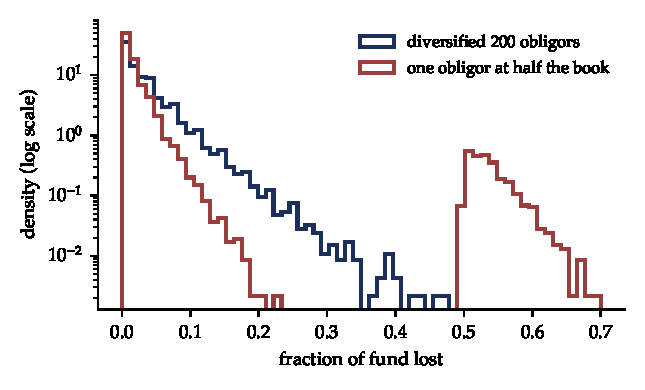
\includegraphics[width=\linewidth]{fig_greensill_loss}
\caption{Simulated distribution of annual losses for a diversified receivables portfolio and for one in which a single obligor accounts for half the book. Both have the same expected loss. Simulation with a one factor Gaussian copula, default probability three per cent and asset correlation $0.2$.}
\label{fig:greensillloss}
\end{figure}

The legal significance is that expected loss, the figure most easily stated, is not the figure an investor in a low risk fund cares about. A representation that a fund holds short dated, insured receivables of investment grade obligors conveys a belief about the whole distribution, in particular that the probability of a large loss is negligible. If the actual portfolio was concentrated, that implied belief was false even if the expected loss was correctly stated. This is a half truth in the sense of \emph{Dimmock v Hallett} \citep{dimmock1866}: the statement is literally consistent with the facts but conveys a posterior the speaker's information does not warrant.

\section{Future receivables as a change of hypothesis}

The second question concerns future receivables. A receivable is a claim on a buyer that has bought goods and promised to pay. A future receivable is an expectation that some buyer will do so. The default probability of a pool of existing receivables from large buyers is low because those buyers are creditworthy and have already incurred the obligation. The default probability of a loan repayable from future sales depends on whether the sales happen, which depends on the client's business, and on whether the proceeds reach the lender.

In the language of Chapter~\ref{ch:bf}, a pool of future receivables is a different hypothesis from a pool of existing receivables, with a different likelihood for repayment. Describing the former as the latter is not a small misstatement of a parameter but a misstatement of the model. The Kullback Leibler measure of Chapter~\ref{ch:misrep} makes this concrete. If the warranted probability of a large loss on a future receivables loan to a weak client is ten per cent and the conveyed probability is one tenth of one per cent, the divergence $D(p\,\|\,q)$ is about $0.37$ nats, nine times the mild overstatement of Chapter~\ref{ch:misrep} (about $0.04$ nats) though well short of its gross one (about $1.6$ nats).

\section{Updating on payment history}

The third question is what a lender or investor monitoring the portfolio should have inferred from its performance. Suppose an obligor's payments are observed over time and some are late or rolled over. A simple model treats each settlement as a Bernoulli trial with probability $\phi$ of difficulty. With a beta prior reflecting an initially favourable view, say $\text{Beta}(1,30)$ with mean about three per cent, a record of two late settlements in twelve moves the posterior mean to about seven per cent; six in twenty four moves it to about thirteen per cent (Figure~\ref{fig:greensillbeta}).

\begin{figure}[t]
\centering
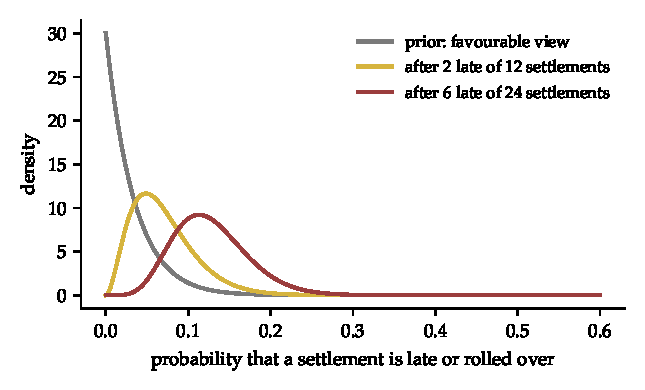
\includegraphics[width=\linewidth]{fig_greensill_beta}
\caption{Posterior distributions for the probability that an obligor's settlement is late or rolled over, as late or rolled settlements accumulate, starting from a favourable prior. Illustrative.}
\label{fig:greensillbeta}
\end{figure}

When a lender rolls over maturing receivables rather than collecting them, as can happen when a client cannot pay and the lender refinances, the observed record of defaults is censored: problems are concealed by refinancing. A Bayesian monitor should treat rollovers as partial evidence of distress, not as clean repayments. Investigations of Credit Suisse's handling of its Greensill relationship, including the Swiss regulator's 2023 finding that the bank had seriously breached its supervisory obligations \citep{finma2023}, describe internal warnings that were not acted on. The general lesson is that an institution's risk system should update on adverse signals, and that failure to update when the evidence warrants is a failure of epistemic responsibility.\index{Credit Suisse}\index{FINMA}

\section{The insurance questions}

The insurers' position in the litigation that followed was, in broad terms, that the policies were not valid or did not respond, because of non disclosure and other defences. Greensill and the Credit Suisse funds contended otherwise. Many of the principal claims were brought in the Federal Court of Australia. A large claim by Credit Suisse funds against the insurer Insurance Australia was reported settled before trial, in 2026 according to trade press reports. We do not express any view on the merits.

What the Bayesian framework offers is a way to organise the questions such a case raises, using the English law of fair presentation as the template.
\begin{enumerate}[label=(\alph*)]
\item What did the insured know or ought to have known about the risk, $D_S$ in the notation of Chapter~\ref{ch:misrep}?
\item Was that information presented fairly, so that a prudent insurer's posterior on loss would have been what $D_S$ warranted?
\item If not, what posterior would a prudent insurer have formed with a fair presentation, and what decision, premium or terms would it have made?
\item Was any failure deliberate or reckless, in which case the remedy is avoidance, or merely careless, in which case the remedy depends on what the insurer would have done?
\end{enumerate}
Question (c) is a counterfactual. It requires a model of the insurer's underwriting: how it priced risk as a function of concentration, obligor quality and the nature of receivables. The insurer's own underwriting guidelines, pricing models and correspondence are the evidence. A court applying the Insurance Act 2015 would ask the insurer to show the premium it would have charged, and would reduce the claim in proportion. This is an expected utility comparison of the kind Lindley advocated for courts \citep{lindley1991}.

There is a further layer. If the insurer's own underwriter had a relationship with the insured that compromised his independence, the insurer's posterior was formed through a corrupted channel. Whether the insured can rely on cover written by an agent who exceeded his authority, and whether the insurer is bound by what its agent knew, are questions of agency law. In Bayesian terms they ask whose information set defines the insurer's knowledge.

\section{The directors' responsibility}

In June 2026 the Insolvency Service announced that Lex Greensill had given a disqualification undertaking under which he may not act as a director of a company in the United Kingdom for nine years. The undertaking was given days before a six week trial of the Secretary of State's claim, which had sought a longer period; Greensill had earlier failed in an application to strike out the proceedings. An undertaking involves the director not disputing certain facts for the purposes of the disqualification proceedings only. The Insolvency Service's statement said, among other things, that he had caused Greensill companies to enter transactions in late 2020 that removed legal protections underpinning a Credit Suisse fund's investment.\index{director disqualification}

The Company Directors Disqualification Act 1986 requires the court to disqualify a director of an insolvent company whose conduct makes him unfit to be concerned in the management of a company. Unfitness is assessed on the civil standard, but the seriousness of the consequences has led courts to examine the evidence with care. In the language of Chapter~\ref{ch:standards}, the standard is a posterior threshold of one half, and the care reflects a low prior for the most serious allegations rather than a higher threshold. A disqualification undertaking is a settlement: the parties agree on a period in light of their posteriors about the likely outcome of trial and its costs, a subject we model in Chapter~\ref{ch:becker}.

\section{Political access and the value of information}

Greensill's lobbying of government ministers in 2020, on behalf of the company's access to emergency lending schemes, through the former prime minister David Cameron, led to a parliamentary inquiry and a government review. The House of Commons Treasury Committee concluded in 2021 that there had been a significant lack of judgment in the way the former prime minister lobbied, though it found no breach of the lobbying rules as then drafted \citep{treasury2021}. The episode is relevant here for a narrow reason. Access to decision makers is valuable because it lets a party supply information, and selected information, to someone whose decision affects it. The theory of Bayesian persuasion in Chapter~\ref{ch:misrep} applies: a sender who controls the information structure can move a receiver's posterior in its favour without stating a falsehood. Rules on lobbying are, in part, rules about which information structures are permitted.

\section{A Bayesian network for the case}

Figure~\ref{fig:greensillbn} is a simplified Bayesian network for the core inferential questions. The latent variables are the true quality of the asset pool, $Q$, the client concentration, $C$, and whether receivables were existing or prospective, $R$. These determine the default risk $\theta$. The signals are the fund documentation, the insurance cover, and the observed payment history. The insurer's decision to write cover depends on its posterior on $\theta$, which in turn depends on what was presented. The network makes explicit that the presence of insurance is not independent evidence of low risk if the insurance decision was itself based on the same, possibly incomplete, information. Treating the insurance as an additional, independent safety signal double counts.\index{double counting}

\begin{figure}[t]
\centering
\begin{tikzpicture}[node distance=1.0cm and 1.3cm, every node/.style={font=\scriptsize},
 lat/.style={circle, draw=nightblue, fill=softgray, minimum size=8mm, inner sep=1pt},
 obs/.style={rectangle, draw=nightblue, fill=starlight!30, minimum size=7mm, inner sep=2pt, align=center},
 ar/.style={-{Stealth[length=1.6mm]}, nightblue}]
\node[lat] (Q) {$Q$};
\node[lat, right=of Q] (C) {$C$};
\node[lat, right=of C] (R) {$R$};
\node[lat, below=of C] (th) {$\theta$};
\node[obs, below left=1.0cm and 0.6cm of th] (doc) {fund\\ documents};
\node[obs, below=1.0cm of th] (ins) {insurance\\ cover};
\node[obs, below right=1.0cm and 0.6cm of th] (pay) {payment\\ history};
\node[obs, left=1.6cm of th] (pres) {presentation\\ to insurer};
\draw[ar] (Q) -- (th); \draw[ar] (C) -- (th); \draw[ar] (R) -- (th);
\draw[ar] (th) -- (pay);
\draw[ar] (Q) -- (pres); \draw[ar] (C) to[bend right=35] (pres);
\draw[ar] (pres) -- (ins);
\draw[ar] (pres) -- (doc);
\draw[ar] (ins) -- (doc);
\end{tikzpicture}
\caption{A simplified Bayesian network for the Greensill inference problem. The insurance cover depends on the presentation, not directly on the true risk, so it is not an independent signal of low risk.}
\label{fig:greensillbn}
\end{figure}

\section{Loss and causation}

If a court were to find that investors were induced by misrepresentation to buy notes, it would need to assess loss. The measure in deceit, and under section 2(1) of the Misrepresentation Act 1967, is the loss flowing from entering the transaction, comparing the investor's position with where it would have been had it not invested. In negligent misstatement, after the Supreme Court's decision in \emph{Manchester Building Society v Grant Thornton}, the court asks about the scope of the duty: what risk the adviser was responsible for guarding against, and whether the loss falls within it \citep{mbs2021}. In Bayesian terms, scope of duty asks which component of the investor's posterior the defendant undertook to get right. A fund manager who undertook to describe the composition of the portfolio is responsible for losses that flow from its concentration; an insurer responsible only for paying claims under the policy is not responsible for losses from uninsured risks.

Proportionality arises again. Suppose investors would have invested in a fund correctly described as holding concentrated and partly prospective receivables, but at a higher yield. The loss attributable to the misrepresentation would then be, on a Bayesian view, not the whole loss but the difference between the outcome and what they would have accepted at a fair price. This is the counterfactual decision analysis of the Insurance Act applied to investment: the remedy should reflect the decision the claimant would have made with a correct posterior.

\section{Lessons}

Greensill teaches four lessons that recur in this book.

First, chains of reliance weaken information. Each additional party that passes on another's assessment adds noise and possibly bias, and the final recipient's posterior should reflect the weakest link. Legal doctrines of reliance and scope of duty allocate responsibility along such chains.

Second, the shape of the loss distribution matters as much as its mean. Representations about safety are representations about tails. The law of misrepresentation should judge them by what they imply about the probability of large losses, not only expected losses.

Third, signals that are not independent should not be added. Insurance written on the originator's presentation is not an independent check on the originator. Courts and regulators should ask what each signal adds given the others.

Fourth, the Bayesian remedy is counterfactual and proportional. English insurance law has adopted it. The law of misrepresentation in investment would benefit from doing the same. Chapter~\ref{ch:bankruptcy} turns to the bankruptcy courts, where the same questions about what was knowable at the time of a transaction arise in a different form.

\section*{Notes and Questions}
\addcontentsline{toc}{section}{Notes and Questions}
\begin{enumerate}[label=\arabic*.]
\item Using a one factor Gaussian copula, compute the probability that a portfolio with one obligor at fifty per cent of the book loses more than forty per cent in a year, for default probabilities of one, three and five per cent. Comment on the sensitivity.
\item Write a short representation that a fund manager might make about a supply chain finance fund. Identify the implied beliefs about the loss distribution. Which facts about the portfolio would make the representation a half truth?
\item In the beta model of this chapter, how many on time settlements would be needed after six late settlements in twenty four to bring the posterior mean back below five per cent?
\item An insurer charged $0.4$ per cent for cover; a fair presentation would have led it to charge $1.2$ per cent. A claim of fifty million pounds is made. What does the insurer pay under Schedule 1 of the Insurance Act 2015 if the breach was careless? If it was reckless?
\item Explain, using the network in Figure~\ref{fig:greensillbn}, why the presence of insurance should not be treated as independent evidence of low risk by an investor. When could it be?
\item Read the Insolvency Service's statement of June 2026 on the disqualification undertaking. Which of the facts stated bear on epistemic responsibility and which on decision responsibility?
\end{enumerate}

\section*{Further reading}
Our tort paper uses Greensill as its main example \citep{polson_sokolov_tort}. The House of Commons Treasury Committee report \emph{Lessons from Greensill Capital} (2021) and the Swiss regulator's 2023 statement on Credit Suisse are the main official accounts \citep{treasury2021,finma2023}.

\chapter{Bankruptcy, Solvency and Hindsight}
\label{ch:bankruptcy}

\section{The question bankruptcy courts ask}

When a firm fails, its creditors look backwards. A leveraged buyout two years earlier paid hundreds of millions of dollars to the old shareholders and loaded the company with debt. A dividend was paid shortly before the collapse. A parent company sold a subsidiary to the debtor at a high price, or took its assets for a low one. Bankruptcy law lets a trustee or creditors' committee claw back such transfers if they were fraudulent, either because they were made with actual intent to hinder, delay or defraud creditors, or because they were constructively fraudulent: made for less than reasonably equivalent value at a time when the debtor was insolvent, was left with unreasonably small capital, or intended or believed it would incur debts beyond its ability to pay. Section 548 of the United States Bankruptcy Code states these tests, and state law versions under the Uniform Fraudulent Transfer Act and its successor, the Uniform Voidable Transactions Act, are available to the trustee through section 544(b). English law has analogous provisions on transactions at an undervalue and preferences in the Insolvency Act 1986.\index{fraudulent transfer}\index{solvency tests}

Each of the financial tests is a statement about the future made at a moment in the past. Was the debtor insolvent on the date of the transfer, meaning that the fair value of its assets was less than its debts? Was its capital unreasonably small for the business it was about to conduct? Would it be able to pay its debts as they matured? None of these can be answered by looking at what later happened, since the firm's failure is the reason the question is being asked, and a court that reasons from the failure to the earlier insolvency commits the error of hindsight. Each must be answered with the information available at the time. That makes solvency a probability judgment conditioned on a past information set, and it makes bankruptcy litigation a natural home for Bayesian reasoning.

J. B. Heaton, a Chicago lawyer and financial economist with whom one of us has also written on deep learning in finance \citep{heaton2017}, has argued that legal solvency tests should be understood through financial economics, and that the right test depends on the context in which it is applied \citep{heaton2002,heaton2007}. This chapter develops his argument in Bayesian terms and works through the principal cases.

\section{Three tests as three posteriors}

\subsection{The balance sheet test}

The balance sheet test asks whether the fair value of the debtor's assets exceeded its liabilities. Fair value is not book value: it is what the assets would fetch in an orderly sale, or the value of the business as a going concern. For a firm whose assets are its future cash flows, fair value is the present value of those cash flows, which depends on forecasts. In financial economics the natural measure is the market value of the firm's enterprise, the sum of the market values of its debt and equity.\index{balance sheet test}

Heaton's first point is that the balance sheet test, read literally, asks the wrong question for a going concern. A firm whose enterprise value is slightly below the face value of its debt is not necessarily doomed. Its equity still has value as an option on the upside, and creditors may be paid in full if things go well. Conversely, a firm whose enterprise value exceeds its debt may face a high probability of default if its assets are volatile. What matters to creditors is the probability and severity of default, not a point comparison of two numbers.

\subsection{The Merton model}

Merton's structural model of credit risk makes this explicit \citep{merton1974}. Let $V_t$ be the value of the firm's assets at time $t$. Treat the firm's assets as following a geometric Brownian motion with volatility $\sigma$, and its debt as a single zero coupon bond with face value $D$ maturing at $T$. Equity is a call option on the assets with strike $D$. The probability, under the real world measure with drift $\mu$, that the firm defaults at $T$ is
\begin{equation}
\Prob(V_T < D) = \Phi\left(-\frac{\log(V_0/D) + (\mu - \sigma^2/2)T}{\sigma\sqrt{T}}\right).
\label{eq:merton}
\end{equation}
Here $\Phi$ is the standard normal cumulative distribution function, the probability that a standard normal variable falls below its argument. Figure~\ref{fig:merton} plots \eqref{eq:merton} as a function of leverage. In the parameterisation of the figure, with an asset drift of three per cent, a firm with debt equal to ninety per cent of asset value has a one year default probability of about one in five if its asset volatility is fifteen per cent, and of nearly one half if it is fifty per cent. The balance sheet test treats both as solvent.\index{Merton model}

\begin{figure}[t]
\centering
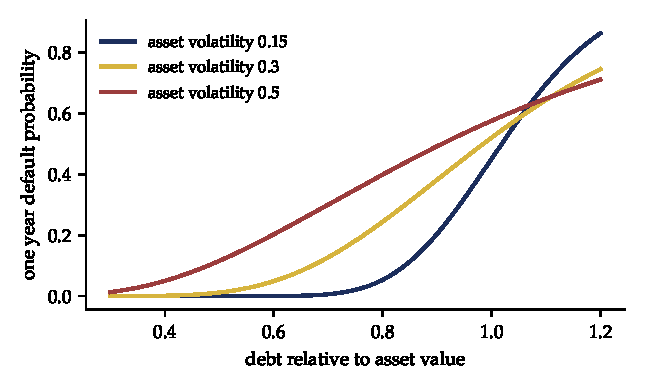
\includegraphics[width=\linewidth]{fig_merton}
\caption{One year default probability in the Merton model as a function of leverage, for three asset volatilities. The balance sheet test draws a line at leverage of one; the probability of default changes smoothly and depends heavily on volatility.}
\label{fig:merton}
\end{figure}

\subsection{Unreasonably small capital and ability to pay}

The unreasonably small capital test and the ability to pay test are forward looking by design. Courts have described the first as asking whether the debtor had sufficient capital to withstand reasonably foreseeable difficulties, and have said that it requires an assessment of the reasonableness of the debtor's projections at the time. In \emph{Moody v Security Pacific Business Credit}, the Third Circuit held that the test looks to the ability to generate sufficient profits to sustain operations, and that projections must be reasonable and prudent when made \citep{moody1992}. In Bayesian terms, both tests ask whether the posterior probability of failing to meet obligations over a relevant horizon, given information at the transfer date, was unacceptably high.

What is unacceptably high? The statute does not say. Heaton argues that this is the right place to recognise that the tests serve different purposes in different contexts. Fraudulent transfer law protects creditors against transfers that shift risk to them without their consent. A transfer that raises the probability of default from one per cent to two per cent harms creditors less than one that raises it from ten to forty. A Bayesian formulation would make the test a threshold on the probability of default, or better, on the expected loss to creditors caused by the transfer, with the threshold set by the purpose of the rule.

\section{Hindsight}

\subsection{The psychology}

Kamin and Rachlinski showed in a well known experiment that people asked to judge whether a precaution should have been taken assess the probability of the harm much higher, and are more ready to find that the precaution was required, when they know the harm occurred \citep{kamin1995}. Subjects who were told only the facts before a flood judged the risk low; subjects told that a flood occurred judged the same risk, on the same prior information, much higher, even when instructed to ignore the outcome. Hindsight bias is robust, and judges are not immune to it \citep{guthrie2001}.\index{hindsight bias}

In fraudulent transfer litigation hindsight pushes every assessor, including the court, towards insolvency. The case exists only because the debtor failed. The trustee's expert, retained after the failure, builds a valuation as of the transfer date, choosing among many reasonable assumptions about growth, margins and discount rates. It is easy, and not necessarily dishonest, to choose assumptions that look reasonable in light of what is now known. The defendant's expert leans the other way, for partisan reasons rather than hindsight. The court must choose between two valuations, each a sample from a distribution of possible expert opinions, both shaped by their authors' knowledge of the outcome.

\subsection{A model of hindsight}

Let $\pi$ be the true ex ante probability of default given the information at the transfer date, and $F$ the event that the firm later failed. An expert who forms an estimate after observing $F$ and who cannot fully disregard it reports
\begin{equation}
\hat\pi = \pi + \beta\,\mathbb{1}_F + \epsilon,
\end{equation}
where $\mathbb{1}_F$ is one if the firm failed and zero otherwise, with $\beta > 0$ measuring hindsight bias and $\epsilon$ noise. Because the cases that reach court are exactly those with $F = 1$, the court sees $\hat\pi = \pi + \beta + \epsilon$. There are two distortions. The estimate is biased upwards by $\beta$. And the distribution of $\pi$ among litigated cases is itself shifted upwards relative to all transactions, because failure is more likely when $\pi$ is high, which is a selection effect, not a bias: firms that failed did on average have higher ex ante risk. Figure~\ref{fig:hindsight} illustrates the first. A court needs to correct for the first without overcorrecting for the second.

\begin{figure}[t]
\centering
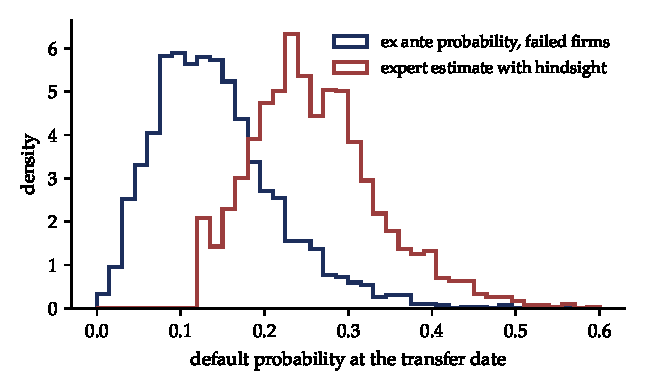
\includegraphics[width=\linewidth]{fig_hindsight}
\caption{Simulated ex ante default probabilities among firms that later failed, and expert estimates of those probabilities formed with knowledge of the failure. The second distribution is shifted to the right by hindsight bias.}
\label{fig:hindsight}
\end{figure}

\section{Market evidence}

\subsection{The market centred paradigm}

Market prices at the transfer date are formed by investors who did not know the outcome. They are free of hindsight bias by construction. If a firm's stock traded at a substantial positive value after the transaction, its bonds traded near par and its credit default swaps were cheap, then the market's posterior on default was low. Courts have increasingly relied on such evidence. Simkovic and Kaminetzky argue that courts should use market implied default probabilities, inferred from credit default swap prices, to assess solvency \citep{simkovic2011}.\index{market evidence}

\begin{casebox}{VFB LLC v Campbell Soup Co (3d Cir. 2007)}
In 1998 Campbell spun off a group of underperforming businesses as Vlasic Foods International, which paid Campbell about five hundred million dollars funded by new debt. Vlasic failed in 2001. Its successor sued Campbell, alleging that Vlasic was insolvent or inadequately capitalised at the spin off. The district court rejected the claim, relying heavily on the market's valuation of Vlasic: after the spin off, Vlasic's equity traded at a market capitalisation of over a billion dollars and its debt was placed with sophisticated lenders. The Third Circuit affirmed, holding that the market's contemporaneous assessment was the best evidence of value, even though Campbell had dressed up Vlasic's results before the spin off, because the market had not been shown to have been misled to the point of making its valuation unreliable \citep{vfb2007}.
\end{casebox}

\begin{casebox}{In re Iridium Operating LLC (Bankr. S.D.N.Y. 2007)}
Iridium launched a satellite telephone system in 1998 and filed for bankruptcy in 1999. The creditors' committee sued Motorola, alleging that Iridium had been insolvent during the period when it paid Motorola large sums. The bankruptcy court rejected the claim after a long trial, relying on Iridium's market capitalisation, the prices of its debt, and the willingness of sophisticated investors to fund it. The court observed that hindsight showed the business plan to have failed, but that the market at the time, with full access to the public information, valued the enterprise well above its debts \citep{iridium2007}.
\end{casebox}

\subsection{The Bayesian view of market evidence}

Market prices are not infallible. They can be distorted by fraud, as the plaintiffs argued in \emph{Campbell}, by thin trading, or by investors' own biases. The Bayesian question is not whether to use them but how much weight to give them relative to other evidence. A coherent approach treats the market implied default probability as one signal and the expert's fundamental analysis as another, each with its own error variance, and combines them. If $\pi_m$ is the market implied probability with error variance $s_m^2$ and $\pi_e$ the expert's uncorrected estimate (the $\hat\pi$ of the hindsight model above), with an assumed hindsight bias $\beta$ and error variance $s_e^2$, a normal approximation with a flat prior, and with the two errors independent, gives the posterior mean
\begin{equation}
\tilde\pi = \frac{\pi_m/s_m^2 + (\pi_e - \beta)/s_e^2}{1/s_m^2 + 1/s_e^2}.
\label{eq:solvencycombo}
\end{equation}
The weights reflect reliability. In a liquid market with no evidence of manipulation, $s_m^2$ is small and the market dominates. If the claimant can show that the market was misinformed, for instance by fraudulent accounts, $s_m^2$ rises, or the market signal must be corrected for the effect of the misinformation. The expert's estimate is discounted for hindsight. Equation \eqref{eq:solvencycombo} is a formal version of the reasoning the courts in \emph{Campbell} and \emph{Iridium} applied when they gave market evidence decisive weight.

\subsection{Credit default swaps}

A credit default swap pays the protection buyer the loss on a reference obligation if the obligor defaults. Its spread $s$, the annual premium, is approximately the risk neutral default intensity times the loss given default:
\begin{equation}
s \approx \lambda^{\mathbb{Q}} (1 - R),
\end{equation}
where $\lambda^{\mathbb{Q}}$ is the default intensity (the annual default rate) under the pricing, or risk neutral, measure $\mathbb{Q}$, and $R$ is the expected recovery rate. A spread of three hundred basis points with forty per cent recovery implies a risk neutral annual default intensity of about five per cent. Risk neutral probabilities exceed real world probabilities because investors demand compensation for bearing default risk, so the implied probability is an upper bound of sorts on the market's actual belief. A Bayesian analysis can model the risk premium explicitly, using historical relations between spreads and realised defaults, to recover a real world posterior. Simkovic and Kaminetzky's empirical work on equity and CDS prices as debtors approach bankruptcy provides the kind of data needed \citep{simkovic2011}.

\section{The leveraged buyout cases}

The largest fraudulent transfer cases arise from leveraged buyouts, in which a company's own assets secure the debt used to buy out its shareholders. If the company later fails, creditors argue that the buyout left it insolvent and that the payments to shareholders should be returned.

\subsection{Tribune}

The Tribune Company was taken private in 2007 in a two step buyout financed with about eleven billion dollars of new debt, and filed for bankruptcy in December 2008. Litigation against former shareholders who received buyout payments ran for more than a decade. In the multidistrict litigation the courts held that many of the claims against shareholders were barred by the safe harbour in section 546(e) of the Bankruptcy Code, which protects settlement payments made by or to financial institutions; the Second Circuit so held in 2019 even after the Supreme Court's decision in \emph{Merit Management v FTI Consulting} narrowed the safe harbour in other respects \citep{tribune2019,merit2018}. The safe harbour is itself a decision rule: Congress chose to protect the stability of securities settlement at the cost of leaving some fraudulent transfers unremedied.\index{Tribune}

\subsection{The decision problem for lenders and directors}

From the point of view of a board considering a leveraged transaction, fraudulent transfer law creates a contingent liability. If the posterior probability that a court will later find the company insolvent is $q$, and the amount clawed back would be $A$, the expected cost is $qA$. Solvency opinions from valuation firms are commissioned to reduce $q$, both by improving the board's information and by creating contemporaneous evidence for later litigation. A Bayesian analysis of a solvency opinion would ask how informative it is: what is the likelihood ratio of a favourable opinion for the proposition that the firm was in fact solvent? If opinion providers almost always give favourable opinions, the likelihood ratio is close to one and the opinion carries little information, whatever its length.

\section{Chapter 11 and the feasibility test}

Bankruptcy law contains other probability judgments. Section 1129(a)(11) of the Bankruptcy Code requires, for confirmation of a Chapter 11 plan, that confirmation is not likely to be followed by liquidation or the need for further financial reorganisation. Courts have said that the plan need not guarantee success, only offer a reasonable assurance of it. This is a posterior threshold. Studies of reorganised firms that later return to bankruptcy, so called Chapter 22 cases, show substantial refiling rates, especially among firms reorganised in Delaware \citep{lopucki2002}. Whether this shows that the threshold courts apply in practice is lenient, which might reflect a judgment about the losses from refusing confirmation, or optimism, is disputed.\index{Chapter 11!feasibility}

The cramdown interest rate is another probability judgment. When a plan is confirmed over the objection of a secured creditor, the plan may give the creditor deferred payments, and if it does they must have a present value equal to the allowed amount of its secured claim, in effect the value of its collateral, which requires a discount rate that reflects the risk of non payment. In \emph{Till v SCS Credit Corp}, a Chapter 13 case, the Supreme Court plurality adopted a formula approach: the prime rate plus a risk adjustment, typically one to three per cent, for the debtor's circumstances \citep{till2004}. A Bayesian would set the risk adjustment from a posterior on the debtor's default probability and the expected recovery, as in the credit spread formula above.

\section{Absolute priority and third party releases}

The absolute priority rule requires that in a cramdown, a dissenting class of unsecured creditors be paid in full before junior classes, including equity, receive anything. Valuation determines who is in the money, and valuation disputes are disputes about posteriors on future cash flows. Senior creditors argue for low valuations, which leave them owning the reorganised firm; junior creditors argue for high ones. The court must choose a value, and the choice transfers wealth. Proposals to replace judicial valuation with market mechanisms, such as auctions or options for junior claimants to buy out senior ones, are in part attempts to replace a judge's posterior with the market's.

In \emph{Harrington v Purdue Pharma} the Supreme Court held in 2024 that the Bankruptcy Code does not authorise a plan to release non debtors, such as the Sackler family, from claims by non consenting creditors \citep{purdue2024}. The decision is about the limits of the bankruptcy court's power rather than about probability, but it changed the expected value of litigation against non debtors and therefore the terms on which future mass tort settlements will be negotiated.

\section{Greensill revisited}

The administrators of Greensill Capital's English companies, and the Credit Suisse funds, have pursued claims arising from the collapse. Several of the issues are of the kind discussed here. Were transactions in late 2020 entered at a time when the companies were insolvent or close to it, and did they prejudice creditors? What was knowable then about the funding position and the insurance? The Insolvency Service's statement on the disqualification undertaking referred to transactions that removed protections for a fund's investment. English insolvency law asks, under section 238 of the Insolvency Act 1986, whether a transaction at an undervalue was entered at a relevant time when the company was unable to pay its debts, and under section 214 whether directors knew or ought to have concluded that there was no reasonable prospect of avoiding insolvent liquidation. Both are posterior probability tests with an information set fixed in the past, and both are exposed to hindsight bias. The methods of this chapter, market evidence where it exists, explicit correction for hindsight, and the combination of signals by their reliability, apply directly.\index{wrongful trading}

\section{Machine learning for solvency}

Altman's Z score, published in 1968, used discriminant analysis on accounting ratios to separate firms that later failed from those that did not, and remains in use. Modern machine learning methods, including deep networks, gradient boosted trees and survival models, predict default from accounting, market and text data often with better accuracy. Work by one of us with Heaton on deep learning in finance discussed how such architectures can learn nonlinear relations among many predictors \citep{heaton2017}. Could a court use them to assess solvency at a past date?

The attraction is obvious. A model trained on thousands of firms, using only information available at each date, is free of the hindsight bias of a litigation expert. It can be audited, and its inputs can be checked. The difficulties are equally real. The model's training data must be from the right population, and a model trained mostly on small firms may be poorly calibrated for a large leveraged buyout. Its output is a probability of default, and the legal tests are not phrased as probabilities, so the court must still choose a threshold. And the model's errors must be understood: a model that is accurate on average may be systematically wrong for unusual structures, such as supply chain finance or special purpose vehicles. A Bayesian approach treats the model's output as another signal in \eqref{eq:solvencycombo}, with an error variance estimated from its out of sample performance on comparable firms.

\section{Summary}

Solvency tests are probability judgments with an information set fixed in the past. Heaton's argument that they should be read through financial economics leads naturally to a Bayesian formulation: insolvency is a high posterior probability of default, or a large expected loss to creditors caused by the transfer, given what was knowable then. Hindsight bias and selection push expert evidence towards insolvency. Market prices are free of hindsight but not of other errors. The coherent response is to combine signals by their reliability, as the courts in \emph{Campbell} and \emph{Iridium} did when they gave market evidence decisive weight, and as machine learning models may soon allow them to do more systematically.

\section*{Notes and Questions}
\addcontentsline{toc}{section}{Notes and Questions}
\begin{enumerate}[label=\arabic*.]
\item Using \eqref{eq:merton} with $\mu = 0.05$, compute the one year default probability for a firm with assets of one hundred, debt of eighty five, and asset volatility of twenty and forty per cent. Would either firm fail the balance sheet test?
\item A firm's CDS spread at the transfer date was four hundred basis points and expected recovery was thirty per cent. Compute the implied risk neutral default intensity. If the real world default intensity is half the risk neutral one, what is the one year probability of default?
\item In \eqref{eq:solvencycombo}, suppose the market implied probability is four per cent with standard deviation two per cent and the expert's estimate is twenty per cent with standard deviation five per cent and an estimated hindsight bias of eight percentage points. Compute the combined estimate. How does it change if fraud doubles the standard deviation of the market signal?
\item Read \emph{VFB v Campbell Soup}. The court relied on market prices even though Campbell had manipulated Vlasic's pre spin off results. Under what conditions should market evidence be discounted for fraud? Express your answer in terms of $s_m^2$.
\item Design a jury or bench instruction on hindsight bias for a fraudulent transfer trial. Would it work? What does the psychological evidence suggest?
\item Section 1129(a)(11) asks whether confirmation is likely to be followed by liquidation. Propose a probability threshold, and justify it by a ratio of losses in the manner of Chapter~\ref{ch:standards}.
\end{enumerate}

\section*{Further reading}
Heaton's articles on solvency tests \citep{heaton2002,heaton2007}; Simkovic and Kaminetzky on market implied default probabilities \citep{simkovic2011}; Kamin and Rachlinski on hindsight \citep{kamin1995}; and the opinions in \emph{Campbell} and \emph{Iridium} \citep{vfb2007,iridium2007}.


\part{Stories, Graphs and Pleadings}
\chapter{Bayesian Stories}
\label{ch:stories}

\section{Why stories}

Trials are won and lost on stories. Counsel open by telling the jury what happened; witnesses are examined to fill in episodes; closing speeches weave the evidence into a narrative that makes sense of it all. Psychological research supports what advocates know. Pennington and Hastie's story model of juror decision making found that jurors construct a narrative from the evidence, evaluate competing narratives by their coverage of the evidence, their coherence and their uniqueness, and choose the verdict that best fits the story they accept \citep{pennington1991}. Wagenaar, van Koppen and Crombag argued that Dutch criminal courts reason by anchored narratives, stories whose episodes are anchored in common sense generalisations \citep{wagenaar1993}. Ronald Allen and Michael Pardo have argued that the law's standards of proof are best understood as comparisons of the relative plausibility of the parties' explanations, rather than as probability thresholds \citep{allen2019}.\index{story model}\index{relative plausibility}

To many lawyers, stories and probabilities seem opposed. Probability is atomistic, treating each item of evidence separately, while stories are holistic. Probability needs numbers, while stories need sense. In our paper with Shiva Maharaj, \emph{Bayesian Stories: Turning Narratives into Evidence}, we argued that the opposition is false \citep{polson_maharaj_stories}. A story is a generative model: a hypothesis about how the evidence came to be. Comparing stories is Bayesian model comparison, and the criteria of the story model, coverage, coherence and uniqueness, correspond to the likelihood, the prior and the concentration of the posterior. This chapter develops the theory and applies it to the murder of Meredith Kercher.

\section{Stories as generative models}

A story $S$ specifies a sequence of events and the causal relations among them. Given $S$, the evidence $E$ has a probability $\Prob(E\given S)$, which may be high if the story predicts the evidence or low if it requires coincidences. Stories have free parameters: the precise times of events, the routes people took, the motives that drove them. Let $\phi$ denote these. Then
\begin{equation}
\Prob(E\given S) = \int \Prob(E\given S, \phi)\,\pi(\phi\given S)\,d\phi .
\end{equation}
Given two stories, the weight of evidence for one over the other, in decibans as in Chapter~\ref{ch:odds}, is ten times the base ten log of the Bayes factor,
\begin{equation}
W(S_1/S_2 : E) = 10\log_{10} \frac{\Prob(E\given S_1)}{\Prob(E\given S_2)},
\end{equation}
and the posterior odds of the stories are the prior odds, based on how plausible each story is before the evidence, multiplied by the Bayes factor.\index{story!as generative model}

This simple formulation captures the three criteria of the story model.

\paragraph{Coverage} A story that explains more of the evidence has higher likelihood. Evidence the story does not explain must be attributed to coincidence, error or some side process, each of which has low probability. A story that leaves a bloodstain unexplained pays for it with a factor equal to the probability of the stain arising by chance.

\paragraph{Coherence} A story whose episodes fit together, whose actors behave in ways consistent with their motives and with common sense, has high prior probability. A story that requires a person to act against his interests, or events to happen in an unusual order, has low prior probability. Coherence is a property of $\pi(S)$ and of $\pi(\phi\given S)$.

\paragraph{Uniqueness} If two stories explain the evidence equally well, neither should be accepted with confidence. In Bayesian terms, the posterior is spread across stories, and the probability of any one of them is limited by the existence of the others. Uniqueness is the requirement that the posterior concentrate on one story.

The Bayesian theory adds two things the psychological model lacks. It gives a common scale on which coverage and coherence trade off: a story that explains one more item at the cost of one more improbable assumption gains or loses depending on the ratio of the probabilities involved. And it penalises stories with many free parameters, through the integral over $\phi$. A story that can be adjusted to fit any evidence has a diffuse prior over its parameters, and its marginal likelihood is low because most of its versions do not fit. This is the Bayesian Occam's razor applied to narratives.\index{Occam's razor}

\section{Stories and the burden of proof}

How do stories relate to the standards of proof? In a criminal case the prosecution offers a story $S_p$ in which the defendant is guilty. The defence need not offer any story, but usually offers one or more, $S_{d,1}, S_{d,2},\ldots$, in which he is innocent. The posterior probability of guilt is
\begin{equation}
\Prob(G\given E) = \frac{\sum_{S \in \mathcal{G}} \Prob(E\given S)\pi(S)}{\sum_{S\in \mathcal{G}\cup\mathcal{I}} \Prob(E\given S)\pi(S)},
\end{equation}
where $\mathcal{G}$ is the set of all stories in which the defendant is guilty and $\mathcal{I}$ those in which he is innocent. This shows why the defence need not prove any story: it suffices that the innocent stories collectively carry enough weight. It also shows the danger of comparing only the stories the parties present. If the prosecution's story is improbable and the defence's story is more improbable still, a naive comparison favours conviction, while a full analysis, including stories nobody told, might not. Lord Brandon's warning in \emph{The Popi M} that a court need not choose between two improbable explanations applies here \citep{popim1985}.

Allen and Pardo's relative plausibility theory says the fact finder should compare the best explanation offered by each side. In a civil case, find for the party whose explanation is more plausible; in a criminal case, convict only if the prosecution's explanation is plausible and there is no plausible explanation consistent with innocence. This is close to the Bayesian theory when one story on each side dominates. It departs from it when the probability is spread across many stories, because the sum over stories can favour one side even when the single best story favours the other.

\section{Hybrid theories}

Bex, van Koppen, Prakken and Verheij developed a hybrid theory combining stories with arguments, in which stories explain the evidence and arguments support or attack the generalisations on which stories depend \citep{bex2010}. Vlek and colleagues proposed building Bayesian networks from scenarios, using idioms for common narrative structures \citep{vlek2014}. Our view is complementary: arguments are claims about likelihoods and priors, and a full Bayesian analysis requires both a set of stories and a set of arguments about their probabilities. The Bayesian theory says how the arguments should be weighed once they are made.

\section{The murder of Meredith Kercher}

\begin{casebox}{The Perugia case}
Meredith Kercher, a British exchange student, was found dead in her locked bedroom in a house she shared in Perugia, Italy, on 2 November 2007. She had been sexually assaulted and stabbed. Her housemate Amanda Knox, an American student, and Knox's boyfriend Raffaele Sollecito were arrested within days, as was Patrick Lumumba, a bar owner whom Knox named during a night interrogation; Lumumba was released when his alibi was confirmed. Rudy Guede, a local man whose DNA and bloody prints were found in the room, was arrested in Germany. Guede, tried separately under a fast track procedure, was convicted and eventually sentenced to sixteen years. Knox and Sollecito were convicted in December 2009, acquitted on appeal in October 2011 after court appointed experts criticised the DNA evidence, had the acquittal annulled by the Court of Cassation in 2013, were convicted again in Florence in 2014, and were definitively acquitted by the Court of Cassation in March 2015, which cited serious flaws in the investigation. Knox's conviction for falsely accusing Lumumba was later the subject of proceedings in Strasbourg, where in 2019 the European Court of Human Rights found that Italy had violated her rights during the interrogation \citep{knox2019}. After that judgment the calunnia conviction was retried in Florence, where Knox was reconvicted in June 2024 (a three year sentence, already served), and the Court of Cassation upheld it on 23 January 2025, ending the case.
\end{casebox}

The Kercher case is ideal for a theory of stories for three reasons. It produced multiple fully reasoned judgments, because Italian courts must give written reasons (\emph{motivazione}) for their verdicts, and these reasons are in effect competing stories. The physical evidence was abundant, contested and subject to independent expert review, so the likelihood ratios of key items can be discussed with some care. And it has been analysed by statisticians, most recently in the comparison of Wigmore charts, Bayesian networks and chain event graphs by Dawid, Kadane, Mortera, Smith and colleagues discussed in Chapter~\ref{ch:classic} \citep{dawid2024kercher}.

\subsection{The stories}

We consider three families of stories.
\begin{description}
\item[$S_1$: Guede alone] Guede entered the house, possibly through the window of another room after breaking it with a rock, encountered Kercher, assaulted and killed her, and left. Knox and Sollecito were at Sollecito's flat.
\item[$S_2$: Guede with Knox and Sollecito] All three were in the house; the assault and killing involved all three; afterwards Knox and Sollecito cleaned some traces and staged the broken window to suggest a burglary.
\item[$S_3$: Knox and Sollecito without Guede] Included for completeness; the extensive evidence of Guede's presence gives it negligible likelihood, and no court accepted it.
\end{description}
The prosecution's story in the trials was a member of $S_2$; the defence's was $S_1$. Within each family the stories differ in detail: the motive offered for $S_2$ changed over the course of the proceedings, and the timing of the attack varied between versions.

\subsection{The evidence}

We focus on the items most discussed. For each we ask how probable it is under $S_1$ and under $S_2$, and report an illustrative weight of evidence in decibans. These numbers are not findings; they are the kind of numbers a careful analyst might defend, and their purpose is to show how the theory structures the argument. Readers will disagree with some of them, and the exercises invite that disagreement.

\paragraph{Guede's traces} Guede's DNA was found inside the victim and on her bag and clothing, and his bloody hand and shoe prints were in the room. This evidence is expected under both $S_1$ and $S_2$, since both have Guede in the room. Its weight for $S_1$ versus $S_2$ is about zero. It decisively excludes $S_3$.

\paragraph{Absence of Knox's traces in the bedroom} Despite extensive testing, no reliable trace of Knox was identified in the room where the murder occurred, which was full of Guede's traces. Under $S_2$, with three people involved in a violent struggle, one would expect some trace of each participant; under $S_1$ none is expected. The probability of finding no trace of a participant in such a room after such an attack, if she were there, is low, though not negligible if she was careful or the collection was poor. A weight of perhaps ten to fifteen decibans for $S_1$ is defensible.

\paragraph{The kitchen knife} A knife from Sollecito's kitchen was found to have Knox's DNA on the handle, expected since she used his kitchen, and on the blade a trace that the police laboratory attributed to Kercher. The court appointed experts on appeal (Conti and Vecchiotti) found that the testing did not follow the internationally recommended precautions for low copy number samples and concluded that the result was unreliable and that contamination could not be excluded. The knife did not match some of the wounds or a bloody imprint on the bed sheet. In the terms of equation~\eqref{eq:lowtemplate} in Chapter~\ref{ch:bf}, the likelihood ratio is bounded by the reciprocal of the probability of contamination or misattribution, $1/c$. If $c$ is one in fifty, the weight for $S_2$ is at most about seventeen decibans; if the result is unreliable, it is close to zero. The question is how likely the reported result is under $S_1$, and given a low copy number sample tested without the standard controls in a laboratory that processed many items from the same victim, it is not negligible.

\paragraph{The bra clasp} A clasp cut from the victim's bra was collected from the floor of the room forty six days after the murder, having been moved and left in place during earlier searches, and was found to carry a trace attributed to Sollecito among a mixture of several contributors. The appeal experts emphasised the long delay, the evident disturbance of the scene and the handling of the item. Under $S_1$, the probability of a trace attributed to Sollecito appearing on an item collected so late from a heavily disturbed scene, where he had been present as the boyfriend of a housemate, is again bounded below by the contamination probability. Its weight for $S_2$ is modest and uncertain.

\paragraph{The broken window} The prosecution argued that the window of a second bedroom had been broken from inside to stage a burglary, citing glass on top of scattered clothing and the height and difficulty of the climb. The defence argued that Guede had a history of entering buildings by breaking windows, and that the climb was feasible. Under $S_1$ the broken window is part of the burglary; under $S_2$ it is staging. Each side's argument concerns the likelihood of details given each story. A weight near zero, with wide uncertainty, seems fair.

\paragraph{Knox's statements} During a long night interrogation, without a lawyer and with a police interpreter, Knox signed statements placing herself in the house and naming Lumumba, an innocent man, as the killer. She retracted them within hours in writing. The statements are the most contested evidence in the case. Knox was denied a lawyer at the 5:45am interview; in April 2008 the Court of Cassation ruled that the statements could not be used against her on the murder charge, though they remained usable on the charge of falsely accusing Lumumba, and the European Court later found a violation on the same ground; we keep them in the analysis to show how such evidence would be weighed. Under $S_2$, a statement placing her at the scene is a partial confession. Under $S_1$, it is a false statement produced by interrogation pressure, a phenomenon well documented in the literature on false confessions (Chapter~\ref{ch:evidence}). The fact that the statement named an innocent man with an alibi, that is, that it was false in a central particular, is evidence about its reliability. Its weight is a matter of judgment; a careful analyst would discount it heavily, and the European Court's later finding about the interrogation supports that discount.

\paragraph{Behaviour} Much was made at trial of Knox's demeanour: doing cartwheels at the police station, kissing Sollecito outside the house. Behaviour of this kind is common among innocent and guilty people under stress, and its likelihood ratio is close to one. Its prominence at trial is an example of the vivid evidence that people overweight (Chapter~\ref{ch:evidence}).

\paragraph{Mixed DNA in the bathroom} Mixed DNA of Knox and the victim was found in the bathroom the two shared. Under both stories this is expected; its weight is near zero.

\begin{table}[t]
\centering\small
\begin{tabular}{p{4.6cm}r}
\toprule
Item & Weight for $S_1$ over $S_2$ (db)\\
\midrule
Guede's traces & $0$\\
No reliable Knox trace in bedroom & $+10$ to $+15$\\
Kitchen knife trace & $-17$ to $0$\\
Bra clasp trace & $-10$ to $0$\\
Broken window & $-5$ to $+5$\\
Interrogation statements & $-5$ to $0$\\
Demeanour & $0$\\
Mixed DNA in shared bathroom & $0$\\
\midrule
Total & $-27$ to $+20$\\
\bottomrule
\end{tabular}
\caption{Illustrative weights of evidence for the lone assailant story against the joint story in the Kercher case. Ranges reflect uncertainty about contamination and reliability. The total adds the weights, which assumes the items are conditionally independent given each story. Not findings of fact.}
\label{tab:kercher}
\end{table}

\subsection{The prior}

The prior compares the plausibility of the stories before the specific evidence. $S_1$ is a burglary that turned into sexual assault and murder by a man whom the defence and press reports described as having a history of breaking into buildings (alleged break-ins, not a burglary conviction). $S_2$ is a joint sexual assault and murder by a young woman with no history of violence, her boyfriend of one week with no history of violence, and a man the woman barely knew, with no clear motive for the two students. The base rate of violent crimes committed jointly by previously non violent young people with a near stranger is low. We take the prior odds of $S_1$ against $S_2$ at more than ten to one, ten decibans or more.

\subsection{The posterior}

Combining a prior of ten decibans with Table~\ref{tab:kercher}, the posterior weight for $S_1$ over $S_2$ ranges from about $-17$ to $+30$ decibans, depending on how one assesses the knife and the clasp. The posterior probability of $S_2$ ranges from about one in a thousand to about ninety eight per cent. This is a large range, and that is the point. The case turned almost entirely on the reliability of two DNA results, the knife trace (a low copy number result) and the bra clasp trace (a mixture), which the appeal experts criticised for contamination, handling and mixture interpretation. Both were processed by the same laboratory, so their weights share a contamination mechanism and are not independent; the sum of the weights is a rough guide only. If they were reliable, the joint story is plausible. If they were not, the evidence for it largely disappears. A trial that focused on the probability of contamination, rather than on the rarity of the profiles or on the defendants' demeanour, would have been addressing the question on which everything depended.

The Italian courts' trajectory can be read in these terms. The first trial court accepted the DNA results and placed weight on behaviour; its posterior favoured $S_2$. The appeal court in 2011, having heard independent experts, concluded that the DNA results were unreliable, which collapsed the case. The Court of Cassation in 2013 criticised the appeal court for, among other things, its treatment of the evidence and its refusal to test a further trace, and sent the case back. The Florence court in 2014 accepted the prosecution's story again. The Court of Cassation in 2015 acquitted definitively, emphasising failures in the investigation. Each court was implicitly assigning different values to the same few likelihood ratios. A Bayesian analysis cannot say which court was right without settling the contamination question, but it can say exactly which question needed settling.

\section{Lessons from Perugia}

Three lessons generalise.

First, the theory of stories identifies the pivotal evidence. Most of the evidence in Perugia was neutral between the stories, however dramatic it seemed. The analysis shows that two items carried the case and that their weight depended on the probability of contamination. A court, or an investigator, should direct resources to the pivotal parameter.

Second, the theory exposes the asymmetric treatment of evidence. Evidence of presence in the shared house, a mixed trace in the bathroom or Knox's DNA on a knife from her boyfriend's kitchen, was presented as incriminating, though it was predicted equally by innocence. Evidence of absence, the lack of Knox's traces in the murder room, was given little weight, though it was predicted far better by innocence. A likelihood ratio analysis treats presence and absence symmetrically.

Third, the theory shows how procedure shapes inference. Under the civil law system, judges and lay assessors deliberate together and must give reasons. The reasons make the implied likelihoods visible and open to appellate review, which is why we can analyse the case at all. The repeated reversals suggest both the value of that transparency and the danger of a system in which each level of court can reweigh the evidence. We return to the comparison with the common law jury in Chapter~\ref{ch:commoncivil}.

\section{Stories and machines}

Large language models are, among other things, story machines. Given a set of facts, they can generate fluent narratives that explain them. This raises an obvious possibility and an obvious danger. The possibility is that a model could generate the set of stories $\mathcal{G}\cup\mathcal{I}$ more completely than human advocates, including stories neither side thought to tell, and so help guard against the error of comparing only two improbable explanations. The danger is that fluent narratives are persuasive in proportion to their coherence, not their likelihood, and a model optimised to produce plausible text is not optimised to produce probable explanations. The Bayesian theory of stories suggests a discipline: every machine generated story should be scored by its likelihood for each item of evidence, with the scores made explicit and open to challenge. Chapter~\ref{ch:pleadings} develops a related generative approach for civil pleadings and Chapter~\ref{ch:lindleyai} for adjudication more generally.

\section*{Notes and Questions}
\addcontentsline{toc}{section}{Notes and Questions}
\begin{enumerate}[label=\arabic*.]
\item Show that if a story $S$ has a free parameter $\phi$ with a uniform prior on an interval of length $L$, and the evidence is consistent with $S$ only for $\phi$ in a subinterval of length $\ell$, then the marginal likelihood is reduced by the factor $\ell/L$. Interpret this as an Occam penalty for a flexible story.
\item Recompute the Kercher posterior with your own weights for each item in Table~\ref{tab:kercher}. Which item is most influential for your conclusion?
\item The knife trace was a low copy number result and was not retested. Suppose a retest would have confirmed the result with probability $0.9$ if it were genuine and with probability $0.2$ if it were contamination. What is the value of information of the retest, in the sense of Chapter~\ref{ch:standards}, for a court with threshold $0.95$?
\item Pennington and Hastie list coverage, coherence and uniqueness. Map each onto the marginal likelihood, the prior or the posterior.
\item Write a short closing speech for each side in a case of your choice, then score each speech by the weights it implicitly assigns to the evidence. Are the speeches coherent?
\item Is there a case in which the relative plausibility theory and the Bayesian theory give different verdicts? Construct one.
\end{enumerate}

\section*{Further reading}
Our paper sets out the theory in more detail \citep{polson_maharaj_stories}. Pennington and Hastie \citep{pennington1991} and Allen and Pardo \citep{allen2019} are the main alternatives. The Dawid et al.\ comparison is the best recent statistical treatment of the Kercher evidence \citep{dawid2024kercher}.

\chapter{Graphical Models of Evidence}
\label{ch:graphs}

\begin{quote}\itshape
Wheresoever there is a cause, there an effect must be produced; this necessity cannot be resisted.
\par\hfill\normalfont Swami Vivekananda, \emph{Karma Yoga}
\end{quote}

\section{From Wigmore to Pearl}

In 1913 John Henry Wigmore published \emph{The Principles of Judicial Proof}, in which he proposed a method for analysing a mass of evidence by drawing a chart \citep{wigmore1913}. Each proposition, whether an item of evidence or an inference from it, was a numbered node; arrows showed which propositions supported which; special symbols marked the force of belief and whether a proposition was offered by the prosecution or defence. Wigmore's charts were neglected for decades, but were revived by Terence Anderson, David Schum and William Twining, whose \emph{Analysis of Evidence} made chart construction a core skill in evidence teaching \citep{anderson2005}.\index{Wigmore chart}

Wigmore's charts are graphs, and since the 1980s graphs have become the organising structure of probabilistic reasoning. Judea Pearl's Bayesian networks represent a joint probability distribution over many variables by a directed acyclic graph together with a conditional probability table for each node given its parents \citep{pearl1988}. The graph encodes conditional independence: each variable is independent of its non-descendants given its parents. This makes inference tractable in large problems and, as important for law, makes the assumptions of an analysis visible. Pearl later extended the framework to causal reasoning, so that a graph can represent not just associations but the effects of interventions and the answers to counterfactual questions \citep{pearl2009}.\index{Bayesian network}\index{Pearl, Judea}

This chapter introduces Bayesian networks for legal evidence, describes Kadane and Schum's analysis of the Sacco and Vanzetti case, catalogues the common patterns or idioms that recur in legal networks, and shows how causal graphs clarify the law of causation in tort.

\section{Bayesian networks in brief}

A Bayesian network on variables $X_1, \ldots, X_n$ is a directed acyclic graph $\mathcal{G}$ and a factorisation
\begin{equation}
\Prob(X_1,\ldots,X_n) = \prod_{i=1}^n \Prob(X_i \given \mathrm{pa}(X_i)),
\label{eq:bnfactor}
\end{equation}
where $\mathrm{pa}(X_i)$ are the parents of $X_i$ in $\mathcal{G}$. Three elementary structures (Figure~\ref{fig:structures}) determine how information flows.

\begin{figure}[t]
\centering
\begin{tikzpicture}[node distance=0.6cm and 0.9cm, every node/.style={font=\small},
 v/.style={circle, draw=nightblue, fill=softgray, minimum size=7mm, inner sep=1pt},
 ar/.style={-{Stealth[length=1.6mm]}, nightblue}]
\node[v] (a1) {$A$}; \node[v, right=of a1] (b1) {$B$}; \node[v, right=of b1] (c1) {$C$};
\draw[ar] (a1) -- (b1); \draw[ar] (b1) -- (c1);
\node[below=0.15cm of b1, font=\scriptsize] {chain};
\node[v, right=1.1cm of c1] (b2) {$B$}; \node[v, below left=0.7cm and 0.3cm of b2] (a2) {$A$}; \node[v, below right=0.7cm and 0.3cm of b2] (c2) {$C$};
\draw[ar] (b2) -- (a2); \draw[ar] (b2) -- (c2);
\node[below=1.15cm of b2, font=\scriptsize] {fork};
\node[v, right=1.9cm of b2] (b3) {$B$}; \node[v, above left=0.7cm and 0.3cm of b3] (a3) {$A$}; \node[v, above right=0.7cm and 0.3cm of b3] (c3) {$C$};
\draw[ar] (a3) -- (b3); \draw[ar] (c3) -- (b3);
\node[below=0.15cm of b3, font=\scriptsize] {collider};
\end{tikzpicture}
\caption{The three elementary structures. In a chain and a fork, $A$ and $C$ may be dependent unless $B$ is observed. In a collider, $A$ and $C$ are independent unless $B$, or a descendant of $B$, is observed.}
\label{fig:structures}
\end{figure}

In a chain $A\to B\to C$, $A$ influences $C$ through $B$; observing $B$ blocks the influence. A motive leads to an act, which leads to a trace; once the act is established, the motive tells us nothing more about the trace. In a fork $A \leftarrow B \to C$, a common cause makes $A$ and $C$ dependent; observing $B$ makes them independent. Two witnesses' reports both depend on what happened; given what happened, they are independent, unless they spoke to each other. In a collider $A \to B \leftarrow C$, two independent causes become dependent when their common effect is observed. If a stain could have come from the defendant or from a contaminated sample, learning that the sample was contaminated lowers the probability that the defendant left the stain. This is explaining away, and it is the structure behind every alternative explanation offered by the defence.\index{explaining away}\index{d-separation}

The general rule, d-separation, says when two sets of variables are independent given a third. A path between them is blocked if it contains a chain or fork node that is observed, or a collider node that is not observed and has no observed descendant. If every path is blocked, the sets are conditionally independent. Lawyers who learn this rule acquire a precise test for whether two items of evidence are independent given the hypothesis, which is the usual condition for adding their weights.

\section{Sacco and Vanzetti}

\begin{casebox}{Commonwealth v Sacco and Vanzetti}
On 15 April 1920 a paymaster and a guard carrying a shoe factory's payroll in South Braintree, Massachusetts, were shot dead by two men who escaped by car with accomplices. Nicola Sacco, a shoe worker, and Bartolomeo Vanzetti, a fish peddler, both Italian immigrants and anarchists, were arrested in May 1920. They were armed when arrested and lied to the police about their associations. They were tried and convicted in 1921 and, after years of motions, appeals and an advisory committee's review, executed in August 1927. The case became an international cause, and debate about their guilt has never ended. In 1977 the Governor of Massachusetts issued a proclamation that the trial had been permeated by prejudice.
\end{casebox}

Joseph Kadane and David Schum's \emph{A Probabilistic Analysis of the Sacco and Vanzetti Evidence} is one of the most thorough Bayesian analyses of a historical trial \citep{kadane_schum1996}. They constructed Wigmore-style charts of the entire body of trial and post-trial evidence, nearly four hundred items, organised around the ultimate propositions that Sacco fired the fatal shot into the guard and that Vanzetti was present. They then converted the charts into inference networks and assessed the required conditional probabilities. Crucially, they did not produce a single answer. Each author assessed the probabilities separately, and they reported both sets, along with sensitivity analyses showing which judgments drove the conclusions.\index{Sacco and Vanzetti}\index{Kadane, Joseph}\index{Schum, David}

The central item against Sacco was the fatal bullet, known as Bullet III, which the prosecution's experts linked to Sacco's pistol: Van Amburgh testified that he was inclined to believe it had been fired from that pistol, while Proctor's testimony was only that it was consistent with having been fired from it; tests by Calvin Goddard in 1927, after the trial, matched it to the pistol. The defence suggested that the bullet in evidence had been substituted. Kadane and Schum's analysis shows how the conclusion depends on the probability of substitution and on the reliability of the ballistic comparison. If one accepts the integrity of Bullet III and the ballistic identification, the evidence against Sacco is strong; if one has serious doubts about either, it is much weaker. The evidence against Vanzetti was much thinner throughout, resting heavily on eyewitness identification and on his possession, when arrested, of a revolver that may or may not have belonged to the dead guard.

Figure~\ref{fig:sacco} is a highly simplified network for the bullet evidence. The ultimate proposition $G_S$, that Sacco fired the fatal bullet, influences whether the bullet recovered from the victim came from Sacco's pistol. The bullet in evidence equals the recovered bullet unless there was a substitution, which may itself depend on whether Sacco was guilty. The expert's report depends on the bullet in evidence and on the reliability of the comparison. Consciousness of guilt evidence, the lies at arrest, depends on guilt but also on Sacco's fear, as an anarchist, of deportation, which provides an alternative explanation.

\begin{figure}[t]
\centering
\begin{tikzpicture}[node distance=0.9cm and 0.7cm, every node/.style={font=\scriptsize},
 v/.style={ellipse, draw=nightblue, fill=softgray, minimum height=6mm, inner sep=2pt, align=center},
 o/.style={rectangle, draw=nightblue, fill=starlight!35, minimum height=6mm, inner sep=3pt, align=center},
 ar/.style={-{Stealth[length=1.6mm]}, nightblue}]
\node[v] (G) {$G_S$: Sacco\\fired};
\node[v, below left=of G] (rec) {recovered bullet\\from Sacco gun};
\node[v, below right=of G] (sub) {substitution};
\node[v, below=1.4cm of G] (evb) {bullet in\\evidence from gun};
\node[v, right=0.6cm of sub] (rel) {comparison\\reliable};
\node[o, below=of evb] (rep) {expert report:\\match};
\node[v, left=1.0cm of G] (fear) {fear of\\deportation};
\node[o, below=of fear] (lies) {lies at\\arrest};
\draw[ar] (G) -- (rec); \draw[ar] (G) -- (sub);
\draw[ar] (rec) -- (evb); \draw[ar] (sub) -- (evb);
\draw[ar] (evb) -- (rep); \draw[ar] (rel) |- (rep);
\draw[ar] (G) -- (lies); \draw[ar] (fear) -- (lies);
\end{tikzpicture}
\caption{A simplified network for the bullet and consciousness of guilt evidence against Sacco. The lies at arrest are a collider: once fear of deportation is established, they say less about guilt.}
\label{fig:sacco}
\end{figure}

\section{Idioms for legal networks}

Building a network for a real case from scratch is laborious. Fenton, Neil and Lagnado proposed a small set of idioms, reusable fragments that capture recurring patterns of legal reasoning \citep{fenton2013}. We describe the most useful.

\subsection{Evidence and accuracy}

An item of evidence $E$ is a report about a hypothesis $H$, and its accuracy $A$ is a separate variable. $E$ depends on both $H$ and $A$. This idiom makes explicit that a witness's testimony is not the fact itself, and that challenges to accuracy are challenges to a parent of $E$, not to $H$. A cross-examination that shows the witness was drunk changes $\Prob(A)$, which changes the likelihood ratio of $E$ for $H$.

\subsection{Cause and consequence}

A hypothesis $H$ causes several observable consequences $E_1, \ldots, E_k$. If the consequences are independent given $H$, their weights add. If they share another common cause, such as a single investigation that produced all of them, they are dependent, and adding their weights double counts.

\subsection{Alternative explanation}

Evidence $E$ has two possible causes, $H$ and an alternative $A$. This is the collider, and it supports explaining away. Every defence of the form that evidence was planted, contaminated or produced by coercion instantiates this idiom.

\subsection{Opportunity and motive}

Opportunity and motive are parents of the act. They raise its prior probability but are not consequences of it. Motive is sometimes treated as evidence of the act in the same way as forensic traces; in the network, motive enters the prior, while traces enter the likelihood.

\subsection{Witness dependence}

Two witnesses who discussed events before testifying are not independent given what happened. In the network there is an edge between them, or a latent variable representing their conversation (Figure~\ref{fig:witness}), and their combined weight is usually less than the sum of their weights. The law's concern with collusion, and the practice of separating witnesses, are attempts to preserve conditional independence.

\begin{figure}[t]
\centering
\begin{tikzpicture}[node distance=0.9cm and 1.2cm, every node/.style={font=\scriptsize},
 v/.style={circle, draw=nightblue, fill=softgray, minimum size=8mm, inner sep=1pt, align=center},
 o/.style={rectangle, draw=nightblue, fill=starlight!35, minimum size=7mm, inner sep=2pt},
 ar/.style={-{Stealth[length=1.6mm]}, nightblue}]
\node[v] (H) {$H$};
\node[o, below left=of H] (W1) {$W_1$};
\node[o, below right=of H] (W2) {$W_2$};
\node[v, below=1.6cm of H] (T) {talk};
\draw[ar] (H) -- (W1); \draw[ar] (H) -- (W2);
\draw[ar] (T) -- (W1); \draw[ar] (T) -- (W2);
\node[v, right=3.4cm of H] (H2) {$H$};
\node[o, below left=of H2] (W3) {$W_1$};
\node[o, below right=of H2] (W4) {$W_2$};
\draw[ar] (H2) -- (W3); \draw[ar] (H2) -- (W4);
\end{tikzpicture}
\caption{Witness idioms. On the right, two witnesses are independent given the event $H$ and their weights add. On the left, a conversation creates dependence, and the combined weight is less than the sum.}
\label{fig:witness}
\end{figure}

\section{Object-oriented networks}

Real cases contain repeated structures: many witnesses, many traces, many suspects. Object-oriented Bayesian networks let the analyst define a class once, such as a witness with its accuracy and testimony, and instantiate it many times. Dawid, Mortera and Vicard used this approach to handle complex DNA problems with many individuals and markers \citep{dawid2007oobn}. The same approach suits legal arguments generally. A class for a document might include its authenticity, its author's knowledge, and its content; a class for an expert might include her qualifications, her methods, and her report.

\section{Graphs for causation in tort}

The law of causation, discussed in Chapter~\ref{ch:tort}, is a natural application of causal graphs. A structural causal model represents each variable as a function of its parents and an independent error term. The intervention $\mathrm{do}(X = x)$ replaces the equation for $X$ with the constant $x$ and propagates the change through the model. The but for question, whether the harm would have occurred without the breach, is a counterfactual (Figure~\ref{fig:twin}): given that the breach and the harm occurred, what would the harm have been under $\mathrm{do}(\text{no breach})$?

Pearl's method for counterfactuals has three steps \citep{pearl2009}. Abduction: update the distribution of the error terms using the evidence of what actually happened. Action: modify the model by the intervention. Prediction: compute the probability of the outcome in the modified model with the updated errors. This makes the but for test computable whenever the model is specified, and it shows why the probability of causation discussed in Chapter~\ref{ch:tort} depends on more than the relative risk: it depends on the joint distribution of the error terms, which data on populations do not fully identify.

\begin{figure}[t]
\centering
\begin{tikzpicture}[node distance=0.8cm and 1.4cm, every node/.style={font=\scriptsize},
 v/.style={circle, draw=nightblue, fill=softgray, minimum size=8mm, inner sep=1pt, align=center},
 u/.style={circle, draw=starlight, fill=white, minimum size=6mm, inner sep=1pt},
 ar/.style={-{Stealth[length=1.6mm]}, nightblue}]
\node[u] (U) {$U$};
\node[v, below left=of U] (X) {breach};
\node[v, below right=of U] (Y) {harm};
\node[v, right=2.6cm of X] (Xc) {no\\breach};
\node[v, right=of Xc] (Yc) {harm\\(cf.)};
\draw[ar] (U) -- (X); \draw[ar] (U) -- (Y); \draw[ar] (X) -- (Y);
\draw[ar] (U) to[bend left=20] (Yc); \draw[ar] (Xc) -- (Yc);
\end{tikzpicture}
\caption{A twin network for the but for test. The left side is the actual world; the right is the counterfactual world in which the breach is removed. Both share the background factors $U$, which are updated by what actually happened.}
\label{fig:twin}
\end{figure}

\subsection{Overdetermination and the NESS test}

Some cases have more than one sufficient cause. Two fires, each sufficient to destroy a house, merge and destroy it. Neither is a but for cause, since the house would have burned without either one. Richard Wright's NESS test treats a condition as a cause if it was a necessary element of a set of conditions sufficient for the outcome \citep{wright1985}. Halpern and Pearl's definition of actual causation formalises a similar idea in structural models, allowing contingencies in which other causes are held fixed \citep{halpern2005}. These definitions address the classic puzzles of overdetermination and pre-emption, and they suggest that the law's departures from the but for test in such cases are principled, although both remain contested.

\subsection{Material contribution as a collider problem}

The mesothelioma cases have a simple graph: the disease has a single trigger, and a latent node records which exposure triggered it, with probability proportional to each employer's dose. Given the disease, the exposures are the parents of that collider, and evidence that one exposure was the trigger explains away the others, consistent with the model of Chapter~\ref{ch:tort}. The posterior probability that a given employer's fibres were responsible is proportional to its share, as in Figure~\ref{fig:fairchild} of Chapter~\ref{ch:tort}. The \emph{Fairchild} exception can be described as a rule for decision when the posterior over causes is spread across several defendants none of whom individually crosses one half.

\section{Graphs as tools of advocacy and judgment}

Graphs are not neutral. Which nodes to include, which edges to draw and which to omit, are choices that reflect a theory of the case. A prosecution graph that omits the possibility of contamination has already decided the most important question. The value of graphical analysis is that these choices are visible, so they can be contested. A court that receives competing graphs from the parties can see where they disagree, and can focus the trial on those points.

The comparison by Dawid and colleagues of Wigmore charts, Bayesian networks and chain event graphs on the Kercher evidence found that each method suits a different user \citep{dawid2024kercher}. Wigmore charts are best for lawyers organising argument; Bayesian networks for forensic scientists computing likelihood ratios; chain event graphs, introduced in Chapter~\ref{ch:classic}, for investigators thinking about how events unfolded.

\section*{Notes and Questions}
\addcontentsline{toc}{section}{Notes and Questions}
\begin{enumerate}[label=\arabic*.]
\item In the collider $A \to B \leftarrow C$ with $A$ and $C$ independent binary variables each with probability $0.1$, and $B = A \lor C$, compute $\Prob(A \given B = 1)$ and $\Prob(A\given B = 1, C = 1)$. Interpret as explaining away.
\item Two witnesses each identify the defendant with likelihood ratio ten: each identifies him with probability 0.9 if he is guilty and 0.09 if he is not. If they spoke to each other, so that the second witness repeats the first with probability one half regardless of what she saw, what is the combined likelihood ratio?
\item Draw a network for the Simpson evidence of Chapter~\ref{ch:classic}, including the battering, the murder, the DNA and the possibility of contamination. Which nodes are colliders?
\item Using the network of Figure~\ref{fig:sacco}, explain why establishing that Sacco feared deportation reduces the weight of his lies at arrest. What would increase it?
\item Construct a structural causal model for \emph{Barnett v Chelsea and Kensington Hospital Management Committee} (Chapter~\ref{ch:tort}). Show how the counterfactual probability of death without the negligence is computed.
\item Explain the difference between the but for test and the NESS test using the two fires example. Which test does English law apply?
\end{enumerate}

\section*{Further reading}
Pearl's \emph{Causality} \citep{pearl2009}; Taroni, Biedermann and colleagues on Bayesian networks in forensic science \citep{taroni2014}; Fenton, Neil and Lagnado on idioms \citep{fenton2013}; Kadane and Schum on Sacco and Vanzetti \citep{kadane_schum1996}; Anderson, Schum and Twining on Wigmore charts \citep{anderson2005}.

\chapter{The Pleadings Game and Generative Bayesian Computation}
\label{ch:pleadings}

\section{Pleading as a game}

Before a civil case reaches trial, the parties exchange written statements of their positions. The claimant states the facts on which the claim rests and the relief sought; the defendant admits, denies or puts the claimant to proof on each allegation, and may raise affirmative defences; the claimant may reply. The purpose of this exchange, in the common law tradition, is to identify the issues: the questions of fact and law on which the parties genuinely disagree and which the court must decide. Everything admitted drops out. Everything denied becomes an issue. A well run pleading process narrows a sprawling dispute to a handful of questions.\index{pleading}

Thomas Gordon's \emph{The Pleadings Game} formalised this process as a dialogue game between two players \citep{gordon1995}. Each player can make moves: assert a claim, concede an opponent's claim, deny it, or offer an argument consisting of premises and a defeasible rule that supports a conclusion. Rules can have exceptions, and a player can challenge a rule by asserting an exception or by arguing that a more specific rule applies. The game ends when no player can make a further relevant move. Its outcome is the set of issues: claims that have been asserted and denied, and that are relevant to the ultimate question, together with the arguments for and against each. Gordon grounded the logic in conditional entailment, a nonmonotonic logic due to Geffner and Pearl, and the procedure in Rescher's formal theory of disputation. His aim was a model of procedural justice: a fair procedure for identifying what is in dispute.\index{Gordon, Thomas F.}\index{Pleadings Game}

In our paper on the Pleadings Game we asked what happens if one adds probabilities to Gordon's structure, and how a modern deep learning system could be built on it \citep{polson_sokolov_pleadings}. The answer leads to generative Bayesian computation, a method for approximating posterior distributions by training neural networks on simulated data. This chapter explains the idea and illustrates it with the pleading standards of English and American law.

\section{From issues to probabilities}

Gordon's game identifies issues but does not say how they will be decided. For a party deciding whether to bring or defend a claim, and for a court managing a case, the next question is how probable each outcome is. Each issue $I_j$ will be resolved for the claimant or the defendant, and the claim succeeds if the issues are resolved in a combination that satisfies the elements of the cause of action. Let $Z_j \in\{0,1\}$ indicate resolution for the claimant. The probability that the claim succeeds is
\begin{equation}
\Prob(\text{success}) = \sum_{z \in \mathcal{S}} \Prob(Z = z),
\end{equation}
where $\mathcal{S}$ is the set of combinations that make out the claim. The structure of $\mathcal{S}$ comes from the substantive law; the joint distribution of $Z$ comes from the evidence the parties expect to adduce and from the way courts decide such questions. A Bayesian network whose structure mirrors Gordon's argument graph, with issues as nodes and rules as edges, gives a natural model for the joint distribution.

\section{Pleading standards as posterior thresholds}

\subsection{Twombly and Iqbal}

In the United States, Rule 8 of the Federal Rules of Civil Procedure requires a short and plain statement of the claim showing that the pleader is entitled to relief. For half a century after \emph{Conley v Gibson} in 1957, this was read as permitting dismissal only if it appeared beyond doubt that the plaintiff could prove no set of facts entitling him to relief. In \emph{Bell Atlantic Corp v Twombly} the Supreme Court in 2007 retired that formula in an antitrust case alleging a conspiracy among telephone companies, holding that a complaint must contain enough facts to state a claim to relief that is plausible on its face \citep{twombly2007}. Allegations of parallel conduct, consistent with conspiracy but equally consistent with independent responses to common market conditions, were not enough. In \emph{Ashcroft v Iqbal} in 2009 the Court extended the plausibility standard to all civil actions and instructed judges to draw on judicial experience and common sense in assessing it \citep{iqbal2009}.\index{Twombly}\index{Iqbal}\index{plausibility pleading}

\begin{casebox}{Bell Atlantic Corp v Twombly, 550 U.S. 544 (2007)}
Subscribers sued the regional telephone companies formed after the breakup of AT\&T, alleging that they had conspired not to compete in each other's territories and to exclude new entrants. The complaint alleged parallel conduct and a statement by one executive, quoted in both the majority opinion and Justice Stevens's dissent, that competing in another company's territory might be a good way to turn a quick dollar but that doesn't make it right. The Supreme Court held the complaint insufficient: parallel conduct is consistent with conspiracy but just as much in line with a wide swath of rational and competitive business strategy unilaterally prompted by common perceptions of the market. The plaintiffs had not nudged their claims across the line from conceivable to plausible.
\end{casebox}

\emph{Twombly}'s reasoning is a likelihood ratio argument. Parallel conduct has roughly equal probability under conspiracy and under independent action in a concentrated market, so its likelihood ratio is near one. Allegations that would move the posterior, such as evidence of meetings or communications, were absent. The Court said that plausibility is not a probability requirement: asking for plausible grounds ``does not impose a probability requirement at the pleading stage'' (\emph{Twombly}), and the standard ``is not akin to a `probability requirement,' but it asks for more than a sheer possibility'' (\emph{Iqbal}). We read the standard nonetheless as an implicit threshold on the posterior probability of the claim given the pleaded facts, taken as true, with the judge's experience and common sense supplying the prior and the likelihoods. The Court's disclaimer denies that a numerical probability must be computed or that the claim must be more likely than not; it does not deny that a complaint whose allegations have a likelihood ratio near one, and so leave the posterior near a low prior, is implausible, and that is all the threshold reading needs. The threshold is lower than the trial standard, since discovery may yet uncover evidence, but higher than the bare possibility contemplated by \emph{Conley}.

The decision theoretic justification for such a threshold is the cost of discovery. In \emph{Twombly} the Court noted that antitrust discovery can be expensive, and that the threat of it can push defendants to settle weak claims. If the cost of discovery is $c$, the value of a successful claim is $V$, and $p$ is the probability of success given the pleaded facts, then on a simple expected value rule the case should proceed when $pV > c$, that is, when $p > p^\ast = c/V$. This threshold rises with $c$ and falls with $V$. A full value of information criterion would also credit discovery with sorting meritorious from unmeritorious claims. The plausibility standard is a rough implementation of the simpler rule, applied without numbers.

\subsection{English strike out and summary judgment}

English procedure reaches similar questions through different routes. Under the Civil Procedure Rules a court may strike out a statement of case that discloses no reasonable grounds for bringing or defending the claim, and may give summary judgment where a party has no real prospect of succeeding and there is no other compelling reason for a trial. In \emph{Swain v Hillman} Lord Woolf said that real prospect means a realistic as opposed to a fanciful prospect \citep{swain2001}. In \emph{Three Rivers District Council v Bank of England (No 3)}, a claim by depositors of the collapsed bank BCCI against the Bank of England for misfeasance in public office, the House of Lords by a majority refused to strike out the claim, holding that the question was whether the claim had no real prospect of succeeding at trial, and that a claim involving disputed facts and serious allegations should generally go to trial \citep{threerivers2001}. The claimants discontinued the action in November 2005, after years of hearings and enormous costs, and were ordered to pay costs on an indemnity basis \citep{threerivers2006}.\index{summary judgment}\index{Three Rivers}

\emph{Three Rivers} is a cautionary example for the decision theorist. The majority's reasoning was that a claim of bad faith against a regulator could not be assessed without hearing the evidence, which is a statement that the value of information from trial was high. The outcome is at least consistent with a low posterior on success and a large cost of the information, though one outcome cannot establish either. A Bayesian assessment at the strike out stage would have had to estimate both. It is not obvious that it would have done better than the House of Lords, but it would at least have made the trade off explicit.

\section{Generative Bayesian computation}

\subsection{The problem}

Suppose we want to compute the posterior probability of success for a pleaded claim, using a model of how disputes of that kind unfold. The model has parameters $\theta$, such as the strength of each issue, the reliability of the evidence each party is likely to have, and the tendencies of courts, and it generates observable data $y$, such as the pleaded facts, the admissions and denials, and the eventual outcome. Bayesian inference requires the posterior $\Prob(\theta \given y)$ and the predictive probability of outcomes. For realistic models these are intractable: the likelihood $\Prob(y\given\theta)$ cannot be written down, because the process that generates pleadings and outcomes is too complex.\index{generative Bayesian computation}

Approximate Bayesian computation and likelihood free inference address this problem by simulation. If we can simulate $y$ from the model for any $\theta$, we can learn the posterior without evaluating the likelihood. Generative Bayesian computation, which we have developed \citep{polson_sokolov_gbc}, does this with neural networks.

\subsection{The method}

The idea is to learn the inverse map from data to parameters directly. Draw $\theta^{(i)}$ from the prior and simulate $y^{(i)}$ from the model, for $i = 1,\ldots, N$, with $N$ large. Then train a neural network $f_w(y, \tau)$, indexed by a quantile level $\tau \in (0,1)$, to minimise the quantile loss for a scalar target $\phi(\theta)$, such as one component of $\theta$ or the probability of success $\Prob(\text{success}\given\theta)$ (the network is trained on one such target at a time)
\begin{equation}
\begin{gathered}
\mathcal{L}(w) = \frac{1}{N}\sum_{i=1}^N \rho_\tau\left(\phi^{(i)} - f_w(y^{(i)},\tau)\right),\\
\rho_\tau(u) = u(\tau - \mathbb{1}\{u < 0\}), \qquad \phi^{(i)} = \phi(\theta^{(i)}),
\end{gathered}
\label{eq:quantileloss}
\end{equation}
with $\tau$ drawn at random for each training example. The minimiser of the expected quantile loss is the conditional quantile function, so after training $f_w(y,\tau)$ approximates the $\tau$ quantile of the posterior of $\phi(\theta)$ given $y$ \citep{polson_sokolov_gbc}. Given a new case with data $y^\ast$, we obtain its posterior by evaluating $f_w(y^\ast, \tau)$ over a grid of $\tau$, or generate posterior draws by evaluating it at uniform random $\tau$. The network approximates Bayesian inference for any data the model could generate, so the cost of training is spread over all future cases, a property called amortisation.

\begin{keybox}
Generative Bayesian computation in four steps.
\begin{enumerate}[label=\arabic*.]
\item Specify a generative model of the dispute: priors on parameters and a simulator for pleadings, evidence and outcomes.
\item Simulate a large training set of parameter and data pairs.
\item Train a quantile network to map data and a quantile level to the corresponding posterior quantile.
\item Apply the trained network to the data of a real case to obtain its posterior.
\end{enumerate}
\end{keybox}

\subsection{A simulator for pleadings}

For the Pleadings Game the simulator generates a dispute in stages. First, latent facts are drawn: what actually happened, encoded as truth values of propositions. Second, each party's knowledge is drawn as a noisy view of the facts. Third, the parties play Gordon's game: the claimant asserts propositions it believes and that support its claim; the defendant concedes those it believes true and whose denial would be costly, denies others, and raises exceptions; the result is a set of issues. Fourth, evidence on each issue is drawn as a noisy signal of the latent facts, with noise depending on the type of issue. Fifth, the court resolves each issue by Bayesian updating on the evidence with a threshold, and the outcome follows from the substantive rules. Parameters $\theta$ include the base rates of the latent facts, the noise levels, and the cost structure that governs concessions.

Training the network on millions of such simulated disputes teaches it to map the observable pleadings, the pattern of assertions, admissions, denials and exceptions, to the posterior distribution of the probability of success, taking $\phi(\theta)=\Prob(\text{success}\given\theta)$ as the target. Admissions are informative because a rational defendant admits what it expects to lose; denials are less informative, because they are cheap; exceptions are informative about which issues the defendant expects to be pivotal. The network learns these regularities from the simulation, and the quality of its inferences depends on the realism of the simulator.

\begin{lstlisting}[language=Python, caption={A sketch of the quantile network for pleadings (the simulator and training loop are omitted).}]
import torch, torch.nn as nn

class QuantileNet(nn.Module):
    def __init__(self, d_in, d_hidden=128):
        super().__init__()
        self.body = nn.Sequential(
            nn.Linear(d_in + 1, d_hidden), nn.ReLU(),
            nn.Linear(d_hidden, d_hidden), nn.ReLU(),
            nn.Linear(d_hidden, 1))
    def forward(self, y, tau):
        return self.body(torch.cat([y, tau], dim=1))

def quantile_loss(theta, pred, tau):
    u = theta - pred
    return torch.mean(u * (tau - (u < 0).float()))

# theta (here the scalar target phi), y simulated from the pleadings model
# for each batch: tau = torch.rand(batch, 1)
# loss = quantile_loss(theta, net(y, tau), tau)
\end{lstlisting}

\section{Case law as training data}

Simulation is only as good as the simulator. The obvious complement is data from real cases: pleadings, motions and outcomes. Large collections of judgments and filings are now available in electronic form in many jurisdictions. Such data can be used in two ways. They can calibrate the simulator, by choosing parameters so that simulated outcomes match observed outcome frequencies for cases with similar pleadings. And they can train a network directly, mapping features of real pleadings to outcomes. The second approach is what commercial litigation analytics products do, typically with discriminative models rather than generative ones.

The Bayesian approach has an advantage over pure prediction from case data: it separates the components of the problem. A discriminative model trained on outcomes learns that certain kinds of claims usually fail, but cannot say why, or how the answer would change if the law changed. A generative model specifies the mechanism, so that one can ask how a change in the pleading standard, or in the cost of discovery, would change outcomes. Since the cases that reach a reported judgment are a selected sample, as the Priest and Klein theory, to which Chapter~\ref{ch:becker} returns, explains, a model that represents the selection process explicitly is needed to learn from them without bias.

\section{Worked example: a negligent misstatement claim}

Consider a claim for negligent misstatement under \emph{Hedley Byrne}, of the kind discussed in Chapter~\ref{ch:misrep}. The elements are a statement, its falsity, an assumption of responsibility, reasonable reliance, breach of the duty of care in making the statement, and loss within the scope of the duty. A simplified pleading exchange might run as follows.
\begin{enumerate}[label=(\alph*)]
\item The claimant pleads that the defendant, its financial adviser, stated that a fund invested only in short dated receivables of investment grade obligors; that the defendant knew the claimant would rely on the statement in deciding to invest; that the statement was false; that a competent adviser would have known it was false; and that the claimant lost money when the fund collapsed.
\item The defendant admits making the statement and knowing the claimant's purpose, does not contest assumption of responsibility or reasonable reliance, denies that it was false when made, denies that a competent adviser would have known otherwise, and pleads that the loss was caused by an unforeseeable event outside the scope of its duty.
\item The claimant replies that the fund held concentrated and prospective receivables at the time of the statement.
\end{enumerate}
The Pleadings Game identifies three issues: falsity at the time of the statement, breach of the standard of care, and scope of duty. A generative model assigns each a prior based on the type of statement and adviser, and a likelihood for the evidence each side is likely to produce. The admission of the statement and of knowledge of reliance, and the decision not to contest assumption of responsibility and reliance, remove three of the six elements from dispute; the specific reply on concentration raises the probability of falsity. A trained network would output a posterior distribution for the probability of success, perhaps centred around one half with substantial spread, reflecting uncertainty about breach and scope. Such an output would help a court decide whether to give summary judgment, and help the parties decide whether to settle.

\section{What the machine adds and what it cannot}

A system of this kind could change civil litigation in three ways. It could make early case assessment cheaper and more consistent, reducing the cost of deciding whether to sue or settle. It could help courts manage dockets by identifying cases likely to settle and issues likely to be pivotal. And it could make the reasoning behind pleading standards more transparent, by showing what posterior a given standard implies.

It cannot replace the judgment of what the law is. The substantive rules that determine $\mathcal{S}$, the combinations of issues that make out a claim, are inputs, not outputs. When the law is uncertain, as it often is at the frontier, the model must represent that uncertainty, and the prior on legal questions is a matter for lawyers. Nor can it guarantee that its simulator captures the world. A network trained on a simulator that omits an important mechanism will be confidently wrong about cases where that mechanism matters. Chapters~\ref{ch:lindleyai} and~\ref{ch:xai} discuss how such systems should be validated and governed.

Gordon called his book a model of procedural justice. Procedural justice requires that parties be heard, that their arguments be considered, and that the decision follow from the arguments in a way they can understand. A Bayesian network built on Gordon's game, and a generative model trained on it, can meet these requirements better than an opaque predictive model, because every probability in the Bayesian network and the simulator can be traced to issues, rules and evidence that the parties themselves put forward.

\section*{Notes and Questions}
\addcontentsline{toc}{section}{Notes and Questions}
\begin{enumerate}[label=\arabic*.]
\item Express the \emph{Conley} standard and the \emph{Twombly} standard as thresholds on a posterior probability, bearing in mind the Court's statement that plausibility is not a probability requirement. What would the threshold have to be for the \emph{Twombly} complaint to survive?
\item Show that the minimiser over $q$ of $\E[\rho_\tau(\theta - q)]$ is the $\tau$ quantile of $\theta$.
\item In the pleading exchange of the worked example, which admissions are most informative about the defendant's own assessment of the case? Model the defendant's decision to admit or deny as an expected cost minimisation.
\item Read \emph{Three Rivers (No 3)}. Write a short opinion applying a value of information test to the strike out application.
\item Design a simulator for a simple contract dispute with two issues, formation and breach. Specify priors and noise levels. What features of the simulated pleadings would a network need to learn the posterior?
\item What biases would a model trained on reported judgments inherit? How could a generative model correct for selection?
\end{enumerate}

\section*{Further reading}
Gordon's \emph{The Pleadings Game} \citep{gordon1995}; our papers on the Pleadings Game and on generative Bayesian computation \citep{polson_sokolov_pleadings,polson_sokolov_gbc}; and the opinions in \emph{Twombly} and \emph{Iqbal} \citep{twombly2007,iqbal2009}.

\chapter{Pleadings in Practice: Worked Cases}
\label{ch:pleadingscases}

\section{From the game to the file}

Chapter~\ref{ch:pleadings} described Gordon's Pleadings Game and our proposal to build a deep generative Bayesian network on it. This chapter applies the method to worked examples drawn from leading cases in five areas: negligence, contract, misrepresentation, employment discrimination and competition. For each we set out the pleaded positions, the issues the exchange produces and, where the facts allow, the probabilities a reasoned analysis would attach to each issue, and the resulting probability of success and value of the claim. The numbers are illustrative, chosen to be defensible on the reported facts; their purpose is to show the method, not to second guess the courts. Each example ends with the step the analysis supports, such as settling, mediating, proceeding to discovery or appealing on a point of law.

The general recipe has six steps.
\begin{enumerate}[label=\arabic*.]
\item List the elements of the cause of action and the available defences.
\item Map the pleadings onto the elements: which are admitted, which denied, which not addressed.
\item For each issue in dispute, assign a prior probability of resolution for the claimant, based on the type of claim and the pleaded facts.
\item Identify dependencies between issues, so that correlated issues are not treated as independent.
\item Compute the probability that the claim succeeds, and the expected recovery.
\item Compare the expected value of continuing with the alternatives, using the costs of each.
\end{enumerate}
The worked examples follow this recipe.

\section{Negligence: a product injury}

\begin{casebox}{The facts, after Donoghue v Stevenson}
A consumer is made ill by a contaminated drink bought by a friend from a retailer. She sues the manufacturer in negligence. She pleads that the manufacturer owed her a duty of care, that it breached the duty by failing to keep its bottling process clean, that the contamination caused her illness, and that she suffered loss.
\end{casebox}

\paragraph{The exchange} The manufacturer admits that it manufactured the drink and that the claimant was ill. It denies that it owed a duty to a consumer with whom it had no contract, denies breach, and denies causation, pleading that the illness may have had another source.

\paragraph{Issues} Duty, breach and causation are in issue; loss is not seriously disputed. After \emph{Donoghue v Stevenson} \citep{donoghue1932}, the duty question is a question of law resolved in the claimant's favour with probability close to one. Breach depends on evidence of the bottling process: the manufacturer controls that evidence, and contamination of a sealed bottle is itself evidence of carelessness. With an inference akin to \emph{res ipsa loquitur}, a prior of about $0.75$ is reasonable. Causation depends on medical evidence: if the illness is of a kind the contaminant produces and the timing fits, about $0.8$.

\paragraph{Dependence} Breach and causation are positively related: evidence that the contaminant was in the bottle supports both. Treating them as independent gives a success probability of $1.0\times 0.75\times 0.8 = 0.6$; allowing positive correlation raises it, perhaps to $0.65$.

\paragraph{Decision} With damages of twenty thousand pounds and costs of fifteen thousand each side under the English rule, the expected value of proceeding is positive for the claimant and the expected cost of defending is high for the manufacturer. A settlement around twelve thousand is in the zone where both gain relative to trial.

\section{Contract: an exclusion clause}

\begin{casebox}{The facts, after Photo Production v Securicor}
A factory owner contracts with a security firm for night patrols. The firm's patrolman, on duty, starts a fire that destroys the factory. The contract contains a clause excluding the firm's liability for any injurious act or default by any employee unless it could have been foreseen and avoided by due diligence on the firm's part. The owner sues for the loss.
\end{casebox}

\paragraph{The exchange} The firm admits the contract, the patrolman's act and the loss. It pleads the exclusion clause. The owner replies that the clause cannot apply to a breach so fundamental, and that it does not on its true construction cover deliberate acts.

\paragraph{Issues} The issue is the construction and effect of the clause. In \emph{Photo Production v Securicor} the House of Lords rejected the doctrine that a fundamental breach automatically defeats an exclusion clause, holding that the question is one of construction, and that between commercial parties of equal bargaining power the clause should be given effect \citep{photo1980}. Before that decision, the owner's argument had substantial support in the Court of Appeal. The probability of the owner succeeding therefore depends on the state of the law: contested while the Court of Appeal applied a rule of law, low after the House of Lords spoke.

\paragraph{The lesson} Pleadings analysis must represent uncertainty about the law as well as the facts. A prior on the legal question, informed by the authorities and the composition of the appellate court, is part of the model. When the law is unsettled, the value of an appeal is high, and the expected value of a claim depends on the probability that the higher court will adopt one view or the other. This is where judgment about precedent enters the Bayesian calculation.

\section{Misrepresentation: an adviser's statement}

\paragraph{The facts} An investment advisory firm tells a client that a fund holds only short dated receivables of investment grade companies. The client invests. The fund collapses, and it emerges that it held concentrated and prospective receivables. The client sues the adviser in negligent misstatement, after \emph{Hedley Byrne} \citep{hedleybyrne1964}. Section 2(1) of the Misrepresentation Act 1967 is not available, since the client contracts with the fund and not with the adviser.

\paragraph{The exchange} The adviser admits the statement and the investment. It denies that the statement was false when made, pleads that it relied on the fund manager's documents, and pleads that the loss was caused by events outside the scope of its duty.

\paragraph{Issues} Falsity at the time of the statement; breach, that is, whether the adviser had reasonable grounds for its belief; and scope of duty and causation. The Greensill analysis of Chapter~\ref{ch:greensill} bears directly. Falsity is likely if the fund's holdings were concentrated at the time, perhaps $0.8$. Breach depends on what a competent adviser would have checked, and the burden is on the claimant; the probability of establishing it might be $0.6$. Scope of duty, after \emph{Manchester Building Society v Grant Thornton} \citep{mbs2021}, depends on whether the adviser undertook responsibility for the composition of the fund, which the statement suggests; $0.7$.

\paragraph{Decision} The claim requires falsity, breach and scope: $0.8\times 0.6\times 0.7\approx 0.34$. With loss of one million pounds, the expected value is about one third of a million before costs. A strike out application by the adviser would fail; summary judgment for either side is inappropriate. Mediation is indicated.

\section{Employment: pleading discrimination}

\begin{casebox}{Swierkiewicz v Sorema N.A., 534 U.S. 506 (2002)}
A Hungarian employee alleged that he was demoted and dismissed because of his national origin and age. The lower courts dismissed his complaint because it did not plead facts establishing a prima facie case under \emph{McDonnell Douglas}. The Supreme Court unanimously reversed, holding that the prima facie case is an evidentiary standard, not a pleading requirement, and that the complaint need only give fair notice of the claim and its grounds \citep{swierkiewicz2002}.
\end{casebox}

\paragraph{After Twombly} \emph{Twombly} \citep{twombly2007} and \emph{Iqbal} \citep{iqbal2009} raised the pleading standard to plausibility\index{plausibility pleading} without overruling \emph{Swierkiewicz}. A discrimination complaint must now plead facts making discrimination plausible, though not a full prima facie case. In Bayesian terms, the complaint must raise the posterior above a threshold given the pleaded facts, taken as true.

\paragraph{An example} A complaint alleges that the claimant, aged fifty eight, was dismissed and replaced by a thirty year old, that her performance reviews were good, and that her manager made remarks about the need for fresh energy. The base rate of age discrimination among dismissals of older workers is modest, perhaps one in ten. The replacement by a much younger worker has a likelihood ratio of perhaps two; good reviews, two; the remarks, three. Treating the three facts as independent given the hypothesis, the posterior odds are $1/9\times 2\times 2\times 3 \approx 1.3$, a posterior probability of about $0.57$. The claim is plausible, clearing any plausibility threshold at or below one half, and should survive a motion to dismiss. Discovery will reveal whether the employer has a documented, non discriminatory reason, which would carry a likelihood ratio favouring the employer.

\section{Competition: pleading conspiracy}

\paragraph{The facts} After \emph{Twombly}, a complaint alleging a price fixing conspiracy must plead more than parallel conduct. Suppose a complaint alleges that four suppliers raised prices by the same percentage within a week, that the increase was not explained by costs, and that senior executives attended an industry meeting shortly before.

\paragraph{The analysis} Parallel price increases in a concentrated market have a likelihood ratio close to one, as the Supreme Court recognised in \emph{Twombly} \citep{twombly2007}. The absence of a cost explanation raises it, perhaps to two. The meeting, which provided an opportunity to agree, multiplies it again, by perhaps three, though meetings are common in many industries. With a prior of one in twenty for collusion in such markets, treating the facts as independent given the hypothesis, the posterior odds are $1/19\times 2\times 3\approx 0.32$, a probability of about one quarter. Whether this suffices depends on the plausibility threshold, which, as Chapter~\ref{ch:pleadings} argued, should depend on the cost of discovery and the value of the claim. A court applying a threshold of one third would dismiss; one applying a threshold of one fifth, in light of the value of the claim, would not. Plus factors such as communications about prices, which have much larger likelihood ratios, are what typically carry such complaints past the motion to dismiss.

\section{A table of decisions}

Table~\ref{tab:pleadingdecisions} summarises the worked examples. The point of the table is not the particular numbers but the structure: each claim reduces to a small number of issues, each issue has a probability, and the decision follows from the combination of probabilities with values and costs. A court managing a docket, a lawyer advising a client and a funder assessing a portfolio all need the same table.

\begin{table}[ht]
\centering\small
\begin{tabular}{p{2.3cm}p{2.9cm}cp{2.0cm}}
\toprule
Claim & Issues in dispute & Success & Indicated step\\
\midrule
Product negligence & breach, causation & $0.65$ & settle\\
Exclusion clause & construction & law dependent & appeal on law\\
Misstatement & falsity, grounds, scope & $0.34$ & mediate\\
Age discrimination & intent & $0.57$ at pleading & proceed to discovery\\
Price fixing & agreement & $0.25$ & depends on threshold\\
\bottomrule
\end{tabular}
\caption{Worked pleadings examples and the decisions they support. Illustrative.}
\label{tab:pleadingdecisions}
\end{table}

\section{Training the network}

The worked examples show what a Bayesian pleadings network must learn: the mapping from the pattern of assertions, admissions, denials and exceptions to probabilities on issues, and from issues to outcomes. Our paper proposes to learn it by simulation from a generative model of disputes, calibrated to data from real cases \citep{polson_sokolov_pleadings}. Each worked example above is one training case, labelled by an expert. A network trained on many thousands of such cases, simulated and real, could produce the table for a new case in seconds, with uncertainty. That is the practical promise: early, consistent and explicit case assessment, available to courts and to parties who cannot afford teams of lawyers to produce it.

\section*{Notes and Questions}
\addcontentsline{toc}{section}{Notes and Questions}
\begin{enumerate}[label=\arabic*.]
\item In the product injury example, construct a joint distribution for breach and causation with marginals $0.75$ and $0.8$ and correlation $0.3$. What is the probability both are found?
\item Before \emph{Photo Production}, what probability would you have attached to the owner's argument? How should a claimant price a claim whose success depends on an unsettled question of law?
\item Recompute the age discrimination posterior with a base rate of one in twenty. Does the claim remain plausible?
\item Identify plus factors that would raise the likelihood ratio of a price fixing complaint above ten. Which could be pleaded before discovery?
\item Take a reported case of your choice and produce a row of Table~\ref{tab:pleadingdecisions} for it.
\end{enumerate}

\section*{Further reading}
Gordon's \emph{The Pleadings Game} \citep{gordon1995}; our paper on the Pleadings Game \citep{polson_sokolov_pleadings}; \emph{Photo Production} \citep{photo1980}; \emph{Swierkiewicz} \citep{swierkiewicz2002}.


\part{Statisticians in the Courtroom}
\chapter{Fienberg and the Evolving Role of Statistics in the Courts}
\label{ch:fienberg}

\section{A statistician in public life}

Stephen Fienberg spent most of his career at Carnegie Mellon University, where he worked on categorical data analysis, log linear models, Bayesian methods, privacy and the census. He also spent an unusual amount of time on the problems of courts and government. He analysed the December 1969 draft lottery (for 1970 induction) and showed that it had not been random \citep{fienberg1971}. He co-chaired the National Research Council's Panel on Statistical Assessments as Evidence in the Courts, whose report, \emph{The Evolving Role of Statistical Assessments as Evidence in the Courts}, appeared in 1989 under his editorship \citep{fienberg1989}. He chaired the Council's committee on the polygraph, whose 2003 report remains the most comprehensive scientific assessment of lie detection \citep{nrc2003}. With Margo Anderson he wrote \emph{Who Counts?}, a history and analysis of the political and legal fights over adjusting the United States census \citep{anderson1999}. And with Jay Kadane he wrote one of the first careful discussions of how Bayesian analyses should be presented in legal proceedings \citep{fienberg_kadane1983}.\index{Fienberg, Stephen}

This chapter is organised around Fienberg's report and the themes it established: how statistical evidence enters litigation, the problems of the adversarial expert, the use of court appointed experts, and the special difficulties of evidence about groups. We then look at four of the domains where Fienberg's own work had legal consequences: jury selection, the draft lottery and the census, and the polygraph.

\section{The 1989 report}

\subsection{Origins and method}

The panel was convened in the mid-1980s, when statistical evidence had become common in American litigation, especially in employment discrimination and antitrust, but when courts and lawyers had little guidance on how to evaluate it. The panel included statisticians, lawyers and judges. Its method was empirical: it studied a set of cases in which statistical evidence had played a large role, examining the expert reports, the testimony and the courts' opinions, and drew lessons from them. The case studies covered employment discrimination litigation, an antitrust price fixing case in which damages were estimated by regression, an environmental dispute in which the evidence concerned risks to health, and identification evidence in a criminal case.

\subsection{Findings}

The panel's main findings, stated in our own words, were these.
\begin{enumerate}[label=(\roman*)]
\item Statistical evidence was becoming more common and more complex, and courts were often ill equipped to evaluate it.
\item The adversarial system tended to produce opposing experts whose analyses differed less in method than in assumptions, and courts found it hard to decide between them.
\item Courts frequently misinterpreted significance tests, treating p values as probabilities that a hypothesis was true and statistical significance as legal significance.
\item The quality of statistical work presented in court varied widely, and professional standards for expert statisticians were weak.
\item Court appointed experts, under Rule 706 of the Federal Rules of Evidence, were underused, and could help courts understand technical disputes.
\item Bayesian methods had a natural place in legal reasoning but required care in presentation.
\end{enumerate}
Each finding remains relevant. The second deserves particular attention.\index{expert witnesses!adversarial}

\section{The adversarial expert}

In a common law trial each party selects and pays its own experts. An expert who reaches conclusions unfavourable to the party that retained her is unlikely to be called. The experts the court hears are therefore a selected sample from the population of possible expert opinions, selected by the parties for favourability. This is a statistical problem, and the panel recognised it as such.

Model it as follows. Let $\theta$ be the true answer to a technical question, such as the damages caused by a price fixing conspiracy. A competent expert, making reasonable choices of method and assumptions, reports $\theta + \epsilon$, where $\epsilon$ reflects those choices and has a distribution with mean zero and standard deviation $\sigma$. Each party consults $k$ experts and calls the one whose report is most favourable. The claimant calls the expert with the largest report, the defendant the one with the smallest. The court sees two order statistics. With normal errors, the expected gap between them grows, to leading order, like $2\sigma\sqrt{2\log k}$ for large $k$, though convergence is slow and the formula overstates the gap at small $k$. A court that splits the difference recovers $\theta$ on average, if the parties search equally hard, but cannot tell from the reports how much of the gap reflects $\sigma$ and how much the parties' search over $k$, and the reports exaggerate the real uncertainty about $\theta$.\index{selection of experts}

The panel's recommendations address this problem in several ways. Requiring experts to disclose their methods and data allows the court to see how much of the disagreement is about assumptions. Court appointed experts provide a draw from the unselected distribution. And professional standards can narrow $\sigma$ by ruling out unreasonable choices. In English procedure, the Civil Procedure Rules state that an expert's overriding duty is to the court (CPR 35.3), allow the court to direct that evidence be given by a single joint expert (CPR 35.7), and permit concurrent evidence (Practice Direction 35, paragraph 11), in which experts give evidence together and respond to each other. Each of these reforms reduces the effect of selection. A Bayesian court would go further and ask each expert to report not a point estimate but a distribution, and to state which assumptions drive it.

\section{Significance and the courts}

The panel found that courts often misread significance tests. Chapter~\ref{ch:bf} explained why: a p value is not the probability that the null hypothesis is true, and the Bayes factor implied by a p value of five per cent is modest. These errors matter most in discrimination cases, where the claim is that an employer's decisions disadvantaged a protected group, and the evidence is a comparison of the group's representation among those hired, promoted or retained with its representation among those eligible.

\subsection{Castaneda v Partida}

\begin{casebox}{Castaneda v Partida, 430 U.S. 482 (1977)}
Rodrigo Partida, a Mexican American, was convicted of burglary with intent to rape in Hidalgo County, Texas. He challenged the composition of the grand jury that indicted him, arguing that Mexican Americans had been systematically excluded. Census data showed that Mexican Americans made up about $79.1$ per cent of the county's population. Over an eleven year period, of $870$ persons summoned to serve on grand juries, only $339$, about $39$ per cent, were Mexican American. The Supreme Court held that this disparity established a prima facie case of discrimination, which the State had not rebutted \citep{castaneda1977}. In a footnote the Court explained that under random selection the expected number would be about $688$ with a standard deviation of about twelve, so the observed number was about twenty nine standard deviations below expectation, and observed that a difference of more than two or three standard deviations would make the hypothesis of random selection suspect.
\end{casebox}

The Castaneda footnote launched the two or three standard deviation rule in American discrimination law. Figure~\ref{fig:castaneda} shows the binomial distribution of Mexican American grand jurors under random selection, with the observed count far in the left tail. In this case the conclusion is not in doubt; the probability of so few Mexican Americans under random selection is astronomically small. The difficulty arises in closer cases.\index{Castaneda v Partida}

\begin{figure}[t]
\centering
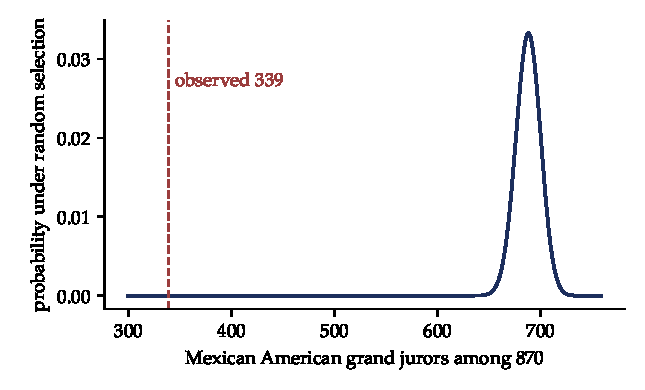
\includegraphics[width=\linewidth]{fig_castaneda}
\caption{The distribution of the number of Mexican American grand jurors among $870$ under random selection from a population that is $79.1$ per cent Mexican American, with the observed count of $339$ marked. The observed count lies about twenty nine standard deviations below the mean.}
\label{fig:castaneda}
\end{figure}

\subsection{The Bayesian analysis}

The binomial test compares the observed count with the distribution under a single hypothesis, random selection. It does not consider any alternative. A Bayesian analysis compares random selection with a hypothesis of discrimination, which must be specified. Suppose under discrimination the probability that a selected juror is Mexican American is $q$, unknown, with a prior distribution on $(0, 0.791)$. The Bayes factor for discrimination against random selection is
\begin{equation}
\BF = \frac{\int_0^{0.791} q^{339}(1-q)^{531}\,\pi(q)\,dq}{0.791^{339}\,(0.209)^{531}}.
\end{equation}
With a uniform prior on $q$, the numerator is dominated by values of $q$ near $0.39$, and the Bayes factor is of the order of $10^{141}$. Any reasonable prior gives an overwhelming result. In a closer case, say $650$ Mexican American jurors out of $870$, about $75$ per cent, which is about three standard deviations below expectation, the Bayes factor depends heavily on the prior for $q$. If discrimination is expected to produce large shortfalls, the modest shortfall is evidence against discrimination; if it is expected to produce small ones, the evidence favours it. This is Lindley's paradox in a discrimination case, and it is why the three standard deviation rule cannot be a complete test.

The Bayesian approach also addresses an issue the binomial test ignores: the relevant population. In \emph{Hazelwood School District v United States} the Court emphasised that the comparison should be with the qualified labour pool, not the general population \citep{hazelwood1977}. For grand juries, eligibility requirements such as literacy and citizenship may differ across groups. Uncertainty about the relevant base rate, as in the Dawid and Mortera analysis of uncertain match probabilities in Chapter~\ref{ch:classic}, should be represented by a prior on the base rate, and it weakens the evidence of discrimination in close cases.

\section{Jury selection and the fair cross section}

The Sixth Amendment guarantees a jury drawn from a fair cross section of the community. In \emph{Duren v Missouri} the Supreme Court set out the test: the excluded group must be distinctive, its representation in venires must be unfair and unreasonable relative to its numbers in the community, and the under representation must be due to systematic exclusion in the selection process \citep{duren1979}. Lower courts measure under representation in several ways, among them absolute disparity, the difference between the group's share in the community and in the venires, and comparative disparity, that difference divided by the group's share in the community. Each has known defects. Absolute disparity understates the problem for small groups; comparative disparity overstates it.

A Bayesian measure avoids these defects by asking a different question: how much does the observed composition of venires change the probability that the process systematically excludes the group, relative to a process that does not? Kadane, in his own work on jury challenges, analysed jury selection data in this way \citep{kadane2008}. The answer depends on the size of the samples, the plausible size of systematic effects, and the base rate, and it can be stated as a Bayes factor, which has the same meaning for large and small groups.

\section{The draft lottery}

In December 1969 the United States Selective Service held a lottery to determine the order in which men born between 1944 and 1950 would be called for military service in the Vietnam War. The 366 days of the year were written on slips, placed in capsules, and drawn from a container. Fienberg showed that the lottery was not random: men born late in the year received systematically lower, and therefore earlier, draft numbers \citep{fienberg1971}. The capsules had apparently been added to the container month by month and not adequately mixed, so December dates, added last, sat near the top. The average draft number for December birthdays was much lower than for January ones, and a simple rank correlation test rejected randomness decisively. The procedure was changed for the next lottery.\index{draft lottery}

The draft lottery is a legal case in the broadest sense. The state was allocating a heavy burden, potentially death, by a procedure whose legitimacy rested on its fairness, and fairness was defined as randomness. A Bayesian treatment would compare the hypothesis of a fair lottery with a family of alternatives in which inadequate mixing produces a trend, and would quantify the evidence for the alternative. More important than the test is the lesson: procedures that are supposed to be random, such as jury selection, case assignment to judges or the allocation of scarce public goods, must be checked, because physical randomisation is harder than it looks.

\section{The census}

The United States Constitution requires an actual enumeration of the population every ten years for the apportionment of seats in the House of Representatives. The census misses some people and double counts others, and the net undercount is larger for some groups than for others. From the 1980s onwards there were proposals to adjust the census using a post enumeration survey, a large sample survey whose results could be used to estimate and correct the undercount by dual system estimation, a capture recapture method. The proposals were fought out in Congress and in the courts.\index{census adjustment}

Anderson and Fienberg's \emph{Who Counts?} tells the story of the 1990 census and the fight over plans for 2000 \citep{anderson1999}. In \emph{Department of Commerce v United States House of Representatives} the Supreme Court held in 1999 that the Census Act prohibits the use of statistical sampling to determine the population for the purpose of apportioning representatives among the states. Sampling remained permitted for other purposes. The legal outcome turned on statutory interpretation, but the underlying dispute was about whether a statistical estimate, with known sampling error and model assumptions, was more or less accurate than an enumeration with known coverage error. A Bayesian analysis would compare the expected loss from each, with the loss defined by errors in apportionment. Fienberg's work showed how such comparisons could be made, and how political interests shaped the willingness to make them.

\section{The polygraph}

The polygraph measures physiological responses (heart rate, blood pressure, breathing and skin conductance) while a subject answers questions, on the theory that deception produces detectable arousal. It has long been excluded as evidence in most American courts, but it is widely used in security screening by government agencies. The National Research Council committee that Fienberg chaired reviewed the scientific evidence and concluded, in 2003, that polygraph testing could discriminate lying from truth telling at rates well above chance but well below perfection, in specific incident investigations with naive subjects, and that the evidence for its use in screening was much weaker \citep{nrc2003}.\index{polygraph}

The committee's most important argument was Bayesian. In employee screening, the base rate of spies among those tested is low. Even a test with high accuracy produces many more false positives than true positives when the base rate is low. Suppose a test detects ninety per cent of spies and clears ninety per cent of non spies, and one employee in a thousand is a spy. In a population of ten thousand, there are ten spies, of whom nine fail the test, and $9{,}990$ non spies, of whom $999$ fail. Of the $1{,}008$ who fail, only nine are spies, less than one per cent. Raising the threshold for failure to reduce false positives also reduces the detection rate. The committee concluded that the polygraph's accuracy in screening was insufficient to justify reliance on it for security decisions. This is the base rate argument of the cab problem in Chapter~\ref{ch:odds}, applied to national security, and it is a model of how Bayesian reasoning should inform public policy on evidence.

\section{Fienberg and Kadane on presentation}

Fienberg and Kadane's 1983 paper in \emph{The Statistician} addressed the question that Tribe had raised: how should a Bayesian analysis be presented in a legal proceeding \citep{fienberg_kadane1983}? Their answer, in brief, was that an expert should present the likelihood function, or the Bayes factor, for the evidence, and show how the posterior would vary over a range of priors, so that the fact finder can supply its own prior. They emphasised that the expert should not present a posterior probability of guilt or liability, because the prior belongs to the fact finder and because a single posterior hides the sensitivity of the conclusion. They also discussed the presentation of uncertainty about the model itself.

\section{Legacy}

Fienberg died in 2016. His work on the courts showed that statisticians could improve legal decisions not by replacing lawyers' reasoning with formulas but by making the structure of the reasoning explicit, testing whether procedures did what they claimed, and insisting on base rates. Chapter~\ref{ch:kadane} turns to his collaborator Jay Kadane, whose work as an expert witness gives a closer view of Bayesian statistics in the courtroom.

\section*{Notes and Questions}
\addcontentsline{toc}{section}{Notes and Questions}
\begin{enumerate}[label=\arabic*.]
\item Verify the Castaneda footnote: compute the mean and standard deviation of the binomial distribution with $n = 870$ and $p = 0.791$, and the number of standard deviations by which $339$ falls short.
\item Compute the Bayes factor for discrimination in a close case of $650$ out of $870$, with a uniform prior on $q$ over $(0.5, 0.791)$ and over $(0.7, 0.791)$. Discuss.
\item In the adversarial expert model, suppose each party consults five experts and calls the most favourable. With $\sigma = 1$, compute by simulation the expected gap between the reports. What would a court learn from a single joint expert?
\item In the polygraph example, find the base rate at which half of those who fail the test are spies.
\item Read \emph{Duren v Missouri}. Propose a Bayesian test for the second element and compare it with absolute and comparative disparity on a small and a large group.
\item The December 1969 draft lottery used physical randomisation. Propose a test of randomness that a court could apply to the assignment of cases to judges. What alternatives should it be powerful against?
\end{enumerate}

\section*{Further reading}
Fienberg's report \citep{fienberg1989}; Fienberg and Kadane on presentation \citep{fienberg_kadane1983}; Anderson and Fienberg on the census \citep{anderson1999}; the polygraph report \citep{nrc2003}; and Finkelstein and Levin's \emph{Statistics for Lawyers} for many worked cases \citep{finkelstein2015}.

\chapter{Kadane on Skill, Chance and the Expert Witness}
\label{ch:kadane}

\section{The working Bayesian}

Joseph Kadane, for many years at Carnegie Mellon, is a Bayesian statistician who has spent a substantial part of his career as an expert witness and consultant in litigation. His casebook \emph{Statistics in the Law} collects many of these engagements with the court documents and commentary: whether electronic draw poker requires skill, the composition of juries, an allegation of copying in an examination, sampling in tax audits, crossing lines in a patent case, the New Jersey Turnpike stops, and others \citep{kadane2008}. His textbook \emph{Principles of Uncertainty} sets out the subjective Bayesian foundations he applies \citep{kadane2011}. With David Schum he produced the probabilistic analysis of the Sacco and Vanzetti evidence discussed in Chapter~\ref{ch:graphs} \citep{kadane_schum1996}.\index{Kadane, Joseph}

Kadane's legal work is instructive because it shows a Bayesian statistician doing the ordinary work of an expert: defining the question in a way the law can use, collecting data, choosing a model the court can understand, and defending conclusions under cross examination. It shows that Bayesian analysis is not only a philosophy of evidence but a practical tool. This chapter concentrates on his work on games of skill and chance, which raises a legal question with a clean statistical structure, and then surveys his other engagements.

\section{Skill and chance in the law}

Gambling is regulated or prohibited in most jurisdictions, and the definition of gambling usually turns on chance. A wager on a game of chance is gambling; a contest of skill with a prize is not. Most games involve both. Courts have adopted several tests to classify them.\index{games of skill}

\begin{description}
\item[Dominant factor test] A game is gambling if chance predominates over skill in determining the outcome. Most American states use some form of this test.
\item[Material element test] A game is gambling if chance is a material element in determining the outcome, even if skill predominates. Some states use this stricter test.
\item[Any chance test] A game is gambling if chance plays any part. Few jurisdictions apply this literally, since almost every contest has some element of luck.
\end{description}
None of these tests says how to measure the contributions of skill and chance. That is a statistical question, and it was the question Kadane was asked in a case about electronic draw poker machines in the 1980s.

\section{Electronic draw poker}

An electronic draw poker machine deals a player five cards; the player chooses which to hold and which to discard; the machine replaces the discards; and the final hand determines the payout according to a fixed table. The cards are dealt at random. The player's only decisions are which cards to hold. Is this a game of skill?

Kadane's approach, described in his contribution to the volume \emph{Statistics and the Law} and reproduced in his casebook, was to compare the results of two strategies \citep{kadane1986,kadane2008}. A dumb strategy, representing a player with no skill, makes the choice of cards to hold at random or by a naive rule. A smart strategy chooses the hold that maximises expected payout. If skill matters, the smart strategy should do much better than the dumb one. Kadane computed, for the payout table at issue, the expected return of each strategy, and found that the smart strategy's expected return was far better than the dumb one's. Choices made a large difference to outcomes, so the game involved substantial skill.

John Lehoczky's comment, and Kadane's rejoinder, both reproduced in the casebook, debated whether this comparison answered the legal question. Even the smart strategy might lose money on average, since the machines are designed to favour the house. Does a game in which skill reduces losses but cannot produce gains count as a game of skill? Kadane's position was that the dominant factor test asks whether skill or chance determines the outcome, not whether a player can win, and that a large difference between strategies shows that outcomes depend substantially on skill. Ware and Kadane developed the analysis further \citep{kadane2008}.

\section{Measuring skill: a Bayesian framework}

The skill question can be put in terms of variance. Let $Y_{ij}$ be the result of player $i$ in hand $j$. A simple random effects model writes
\begin{equation}
Y_{ij} = \mu + \alpha_i + \epsilon_{ij}, \qquad \alpha_i \sim N(0, \sigma_\alpha^2), \quad \epsilon_{ij}\sim N(0,\sigma_\epsilon^2),
\label{eq:skillmodel}
\end{equation}
where $\alpha_i$ is player $i$'s skill and $\epsilon_{ij}$ is luck. In a single hand, the share of variance due to skill is $\sigma_\alpha^2/(\sigma_\alpha^2 + \sigma_\epsilon^2)$. Over $m$ hands, the variance of a player's average result due to luck falls to $\sigma_\epsilon^2/m$, so the share due to skill rises to
\begin{equation}
s(m) = \frac{\sigma_\alpha^2}{\sigma_\alpha^2 + \sigma_\epsilon^2/m}.
\label{eq:skillshare}
\end{equation}
Skill accounts for half the variance when $m = \sigma_\epsilon^2/\sigma_\alpha^2$.
Figure~\ref{fig:skill} plots $s(m)$ for several values of skill variance. Under this model every game with $\sigma_\alpha^2 > 0$ becomes predominantly a game of skill if played long enough. Whether a game is predominantly skill or chance therefore depends on the horizon over which the outcome is judged: a single hand, a session, or a career.\index{skill share}

\begin{figure}[t]
\centering
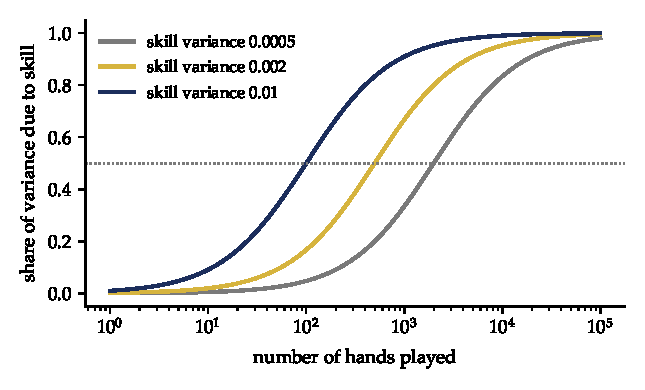
\includegraphics[width=\linewidth]{fig_skill}
\caption{Share of the variance of a player's average result attributable to skill, as a function of the number of hands played, for three levels of skill variance relative to unit luck variance per hand.}
\label{fig:skill}
\end{figure}

This is the crux of many legal disputes over poker. In a single hand of Texas Hold'em, luck plays a large role; a weak player with a strong hand beats a strong player with a weak one. Over thousands of hands, the stronger player wins reliably. Courts that have asked whether chance swamps skill in a single hand have often found poker a game of chance, as the North Carolina Court of Appeals did in \emph{Joker Club v Hardin} in 2007; analyses that look at repeated play find it a game of skill, and Judge Weinstein reached that view in \emph{DiCristina}, discussed below. Courts have split. Miles, Levitt and Rosenfield argued in the \emph{Georgetown Law Journal} that the single hand conception is unduly narrow \citep{miles2013}. Levitt and Miles, using data from the World Series of Poker, showed that players identified in advance as highly skilled earned substantially higher returns than others \citep{levitt2014}.

The Bayesian contribution is to estimate $\sigma_\alpha^2$ and the individual $\alpha_i$ with appropriate uncertainty, using a hierarchical model, and to report the posterior distribution of $s(m)$ for the horizon the law considers relevant. A court can then choose the horizon, which is a legal question, and the statistician can report the skill share for that horizon, which is a factual one.

\section{Simplified poker and the theory of skill}

Larkey, Kadane, Austin and Zamir studied skill in a simplified poker game using computer tournaments among strategies of different sophistication \citep{larkey1997}. A strategy that played randomly, representing zero skill, performed worst; more sophisticated strategies, which took account of the opponent's likely holdings and betting, performed progressively better. Their paper made a conceptual point that is easy to miss: skill in games is relative. A strategy's success depends on the strategies of the other players. A game can reward skill even when no strategy guarantees a profit against every opponent, because a skilled player profits against unskilled ones. In poker, the house takes a fee and players play against each other, so the distribution of skill among players determines who wins.

\section{United States v DiCristina}

\begin{casebox}{United States v DiCristina}
Lawrence DiCristina operated a poker room in Staten Island and was charged under the federal Illegal Gambling Business Act, which applies to businesses that conduct illegal gambling under state law. In 2012 Judge Jack Weinstein of the Eastern District of New York, after hearing extensive expert testimony on skill in poker, including statistical analysis of a large number of online hands, held that poker was predominantly a game of skill and was not gambling within the meaning of the federal statute, and set aside the conviction \citep{dicristina2012}. In 2013 the Second Circuit reversed, holding that the statute covered any business that violated state gambling law, and that poker games of the kind at issue violated New York law, without needing to decide whether poker was a game of skill \citep{dicristina2013}.
\end{casebox}

\emph{DiCristina} shows both the power and the limits of statistical evidence on skill. Judge Weinstein, whose survey of his colleagues on reasonable doubt we met in Chapter~\ref{ch:standards}, engaged with the evidence in detail and was persuaded. The appellate court decided the case on statutory grounds that made the evidence irrelevant. The statistician can answer the factual question, but the legal question of which factual question matters belongs to the courts.

\section{Fantasy sports and online games}

The same issues arose with daily fantasy sports in the 2010s. Operators argued that selecting a fantasy team requires skill and pointed to evidence that a small fraction of players won most of the prizes. Regulators and some courts argued that the outcome of any single contest depends heavily on the unpredictable performance of athletes. In New York, the legislature authorised and regulated interactive fantasy sports in 2016; in 2022 the state's highest court, by a 4 to 3 vote, upheld that legislation against a constitutional challenge, accepting the legislature's judgment that such contests are not gambling within the meaning of the state constitution \citep{white2022}. Three judges dissented. The statistical evidence on skill was relevant but not decisive.

India illustrates a different path. Indian law has long distinguished games of skill from gambling. The Supreme Court held in 1968 that rummy is a game mainly and preponderantly of skill \citep{satyanarayana1968}, and in 1996 that horse racing is a game of skill, so that wagering on it is not gambling \citep{lakshmanan1996}. These decisions were relied on by the online gaming industry, which grew rapidly. In 2025 Parliament enacted legislation prohibiting online money games regardless of whether they involve skill or chance, while promoting other forms of online gaming. The legislature replaced a factual test that courts had applied case by case with a categorical rule. In decision theoretic terms, the legislature can be read as judging that the cost of classification errors and the social harms of money games outweighed the benefit of permitting skill games for money.\index{India!online gaming}

\section{Kadane's other engagements}

\subsection{Jury challenges and peremptory strikes}

Kadane's casebook includes an analysis of a jury challenge in Indiana, \emph{Azania v State}, decided by the Indiana Supreme Court in 2002 on a successive post-conviction petition in a death sentence case, in which the defendant argued that the county jury pool systematically excluded black jurors. The analysis compared the observed representation of black jurors with the expected representation under the selection procedure, taking account of the stages of selection at which under representation could arise \citep{kadane2008}. With Roth and DeGroot, Kadane earlier analysed the sequential game of peremptory challenges, in which prosecution and defence alternately strike prospective jurors without cause, and derived optimal strategies under assumptions about each side's beliefs about jurors' leanings \citep{roth1977}. The analysis showed that the order and number of strikes interact with the parties' information in ways that can be modelled as a Bayesian sequential decision problem. The Supreme Court's later decision in \emph{Batson v Kentucky}, forbidding race based peremptory strikes, created a further statistical question: how to infer discriminatory intent from a pattern of strikes.\index{peremptory challenges}

\subsection{Driving while black}

In \emph{State v Soto}, a New Jersey trial court in 1996 granted motions to suppress evidence obtained in stops of black motorists on the New Jersey Turnpike, finding a pattern of racial targeting \citep{soto1996}. The evidence included surveys of the racial composition of motorists on the turnpike and of those who were speeding, compared with the composition of those stopped. A difficulty was missing data: the race of many stopped motorists was not recorded. Kadane and Terrin analysed the problem of missing data in this context, showing how assumptions about the missing records affected the conclusion and how a Bayesian analysis could represent uncertainty about them \citep{kadane1997}. Their analysis found that the conclusion of disproportionate stops was robust across a wide range of assumptions about the missing data, which is exactly the kind of sensitivity analysis Fienberg and Kadane had recommended in 1983 \citep{fienberg_kadane1983} (Chapter~\ref{ch:fienberg}).\index{State v Soto}

\subsection{Hierarchical models for employment}

Kadane and Woodworth developed hierarchical Bayesian models for employment discrimination cases, in which decisions such as promotions or terminations are made by many decision makers in many units of a firm \citep{kadane2004}. A hierarchical model lets the analyst estimate the effect of a protected characteristic while allowing for variation across units, and can distinguish a firm wide policy from the actions of particular managers. This matters legally, because disparate treatment by a few managers may support individual claims but not a pattern or practice claim. The Supreme Court's decision in \emph{Wal Mart Stores v Dukes}, which rejected class certification in a nationwide sex discrimination case because the plaintiffs had not shown significant proof of a general policy of discrimination, as Rule 23(a)(2) commonality required, turned on exactly this question of whether the variation was firm wide or local.

\subsection{Tax audits and sampling}

With Bright and Nagin, Kadane analysed the use of statistical sampling in tax audits, where an auditor examines a sample of a taxpayer's transactions and extrapolates the error rate to the whole \citep{bright1988}. The legal question is how much the taxpayer should owe given sampling uncertainty. A point estimate overcharges about half the time; a lower confidence bound protects the taxpayer at the cost of undercollection. The decision theoretic answer depends on the relative losses of over and under collection, which is a policy question, but the analysis makes the trade off explicit.

\section{Lessons for the expert witness}

Kadane's career suggests several lessons for statisticians who give evidence.

First, define the question in the law's terms. The court does not need a posterior probability of guilt. It needs an answer to a specific question that the law makes relevant, such as whether skill predominates or whether a disparity is likely due to chance. The statistician's first job is to translate.

Second, use simple models the court can follow, and show that the conclusion is robust to reasonable departures from them. Kadane's poker analysis compared two strategies; his turnpike analysis varied the treatment of missing data. For the turnpike the robustness check carried as much weight as the main result.

Third, be open about the prior. Kadane and Schum reported their separate assessments in the Sacco and Vanzetti analysis. An expert who reports only one prior invites the cross examiner to ask why that one.

Fourth, accept that the law may decide the case on other grounds. \emph{DiCristina} was reversed on the statute; the census case in Chapter~\ref{ch:fienberg} was decided on statutory interpretation. Statistical evidence informs legal decisions but does not dictate them.

\section*{Notes and Questions}
\addcontentsline{toc}{section}{Notes and Questions}
\begin{enumerate}[label=\arabic*.]
\item Using \eqref{eq:skillshare} with $\sigma_\epsilon^2 = 1$ per hand, find the number of hands at which skill accounts for half the variance when $\sigma_\alpha^2 = 0.002$. Should a court assess skill over one hand, one session of three hundred hands, or a year?
\item Design a study to measure skill in a fantasy sports contest. What data would you need, and what model would you fit?
\item In electronic draw poker the house may have an edge even against the optimal strategy. Does this matter under the dominant factor test? Under the material element test?
\item The Indian Supreme Court found rummy to be a game of skill. If you were asked to give evidence, how would you measure skill in rummy?
\item In a pattern of peremptory strikes, a prosecutor strikes four of five black venire members and two of twenty white ones. Formulate a Bayesian test of the hypothesis that race influenced the strikes. What alternative explanations should the model include?
\item Read the casebook materials on electronic draw poker, including Lehoczky's comment and Kadane's rejoinder. Whose argument do you find more persuasive, and why?
\end{enumerate}

\section*{Further reading}
Kadane's \emph{Statistics in the Law} \citep{kadane2008} and \emph{Principles of Uncertainty} \citep{kadane2011}; Larkey, Kadane, Austin and Zamir on skill in games \citep{larkey1997}; Levitt and Miles on poker \citep{levitt2014}.

\chapter{Discrimination, Regression and the Burden of Proof}
\label{ch:discrimination}

\section{Statistics as proof of intent}

Discrimination law asks about the reasons for decisions: whether an employer refused to hire, a lender refused to lend, or a university refused to admit a person because of race, sex or another protected characteristic. Reasons are states of mind, and states of mind are rarely documented. Decision makers do not usually write down that they rejected an applicant because of race. Courts therefore infer intent from patterns. If an employer's hiring of women is far below what the qualified pool would predict, and the employer offers no adequate explanation, the pattern is evidence of discrimination. Statistics have been central to discrimination litigation since the 1970s, and the cases have produced some of the most extended judicial engagements with statistical method in any field of law.\index{discrimination}

This chapter examines that engagement through three questions: how disparities should be measured, how regression analysis should be used to control for legitimate factors, and how the burden of proof structures the inference. It then turns to the litigation over admissions at Harvard, decided by the Supreme Court in 2023, in which the competing regression analyses of two leading economists were at the centre of the trial.

\section{Disparate treatment and disparate impact}

American law distinguishes two theories. Disparate treatment is intentional discrimination: treating a person differently because of a protected characteristic. Disparate impact, recognised in \emph{Griggs v Duke Power} in 1971, is liability for practices that are neutral on their face but fall more harshly on a protected group and cannot be justified by business necessity \citep{griggs1971}. In \emph{Griggs} the employer required a high school diploma and passing scores on aptitude tests for jobs that did not need them, and the requirements excluded black applicants at much higher rates.\index{disparate impact}\index{Griggs v Duke Power}

English law has parallel concepts. Direct discrimination under section 13 of the Equality Act 2010 is treating a person less favourably because of a protected characteristic. Indirect discrimination under section 19 is applying a provision, criterion or practice that puts persons sharing a protected characteristic at a particular disadvantage and cannot be shown to be a proportionate means of achieving a legitimate aim. In \emph{Essop v Home Office} the Supreme Court held that a claimant need not show why the practice disadvantaged the group, only that it did, and that the disadvantage could be established by statistics \citep{essop2017}.

The two theories correspond to two statistical questions. Disparate treatment asks whether the protected characteristic causally affected decisions, holding qualifications fixed: a question about a conditional effect. Disparate impact asks whether a practice produces different outcomes for groups: a question about a marginal difference, followed by a question about justification.

\section{Measuring disparity}

\subsection{The four fifths rule}

The Uniform Guidelines on Employee Selection Procedures, adopted by American federal agencies in 1978, state that a selection rate for any group that is less than four fifths of the rate for the group with the highest rate will generally be regarded as evidence of adverse impact. If seventy per cent of white applicants and fifty per cent of black applicants pass a test, the ratio is $0.71$, below four fifths, and adverse impact is indicated.\index{four fifths rule}

The rule is easy to apply and ignores sampling variation. With small numbers of applicants, a ratio below four fifths can easily occur by chance; with large numbers, a ratio of $0.9$ may be highly significant but not substantively important. Courts have therefore combined the four fifths rule with significance tests, following the standard deviation analysis of \emph{Castaneda} and \emph{Hazelwood} discussed in Chapter~\ref{ch:fienberg}.

\subsection{A Bayesian measure}

A Bayesian approach models the selection rates of the two groups, $\theta_1$ and $\theta_2$, with prior distributions, updates them with the observed counts, and reports the posterior distribution of the ratio $\theta_2/\theta_1$. The posterior probability that the ratio is below four fifths answers the question the rule is trying to ask, while accounting for sampling uncertainty. With beta priors and binomial data the posterior is easily computed. For small samples the posterior is wide, and the probability that the ratio is below four fifths may be modest even when the observed ratio is well below it. For large samples it concentrates near the observed ratio. This measure has the same interpretation at every sample size, although at small samples the posterior depends materially on the prior.

\section{Regression and its discontents}

\subsection{Controlling for qualifications}

Raw disparities do not establish discrimination if groups differ in relevant qualifications. Regression analysis estimates the effect of the protected characteristic on outcomes while controlling for qualifications. In \emph{Bazemore v Friday} the Supreme Court held that a regression analysis need not include every measurable variable to be admissible; the omission of some variables goes to its weight, not its admissibility \citep{bazemore1986}. Since then, regression has been the standard tool in pattern and practice cases.\index{regression evidence}\index{Bazemore v Friday}

\subsection{Omitted variables}

A regression coefficient on a protected characteristic estimates discrimination only if the controls capture all legitimate factors correlated with the characteristic. If a relevant qualification is omitted and is correlated with group membership, the coefficient is biased. Defendants routinely argue that the plaintiff's regression omits important variables; plaintiffs reply that the omitted variables would not change the result. A sensitivity analysis can quantify the dispute: how strongly would an omitted variable have to be related to both the outcome and group membership to explain away the estimated effect? Methods developed by Rosenbaum and, more recently, by Cinelli and Hazlett report the strength of confounding needed to change a conclusion \citep{cinelli2020}. A court can then ask whether a confounder of that strength is plausible, a question about priors.

\subsection{Included variables}

The opposite problem is equally important and less recognised. Including a variable that is itself affected by discrimination removes from the coefficient the part of the effect that runs through that variable, which usually biases it toward zero, and can bias it in either direction if that variable also depends on unmeasured qualifications. If an employer discriminates in assigning initial job grades, and a regression of pay on sex controls for grade, the regression will find little pay discrimination, because the discrimination has been absorbed into the grade. Statisticians call such a variable a mediator, and controlling for it a bad control. Whether to include a variable depends on whether it is a legitimate qualification determined independently of the decision under review, or a product of the same process. This is a causal question, best represented with a graph of the kind discussed in Chapter~\ref{ch:graphs}. The variable lies on a path from the protected characteristic to the outcome; controlling for it blocks part of the effect.

\section{SFFA v Harvard}

\begin{casebox}{Students for Fair Admissions v President and Fellows of Harvard College}
Students for Fair Admissions sued Harvard in 2014, alleging that its undergraduate admissions process discriminated against Asian American applicants. The case was tried in 2018 in the District of Massachusetts. The central evidence consisted of Harvard's admissions data for several cohorts, analysed by two economists: Peter Arcidiacono for SFFA and David Card for Harvard. Both estimated logistic regression models of admission on applicant characteristics. Arcidiacono's models found a statistically significant penalty for Asian American applicants relative to white applicants with similar characteristics. Card's models found no significant penalty. The district court, after a three week trial, found that Harvard had not intentionally discriminated against Asian American applicants \citep{sffa2019}, and the First Circuit affirmed. In 2023 the Supreme Court, deciding this case together with a challenge to the University of North Carolina's admissions, held that race conscious admissions programmes at both universities violated the Equal Protection Clause (and, for Harvard, Title VI, which the Court read to impose the same standard), on grounds that did not depend on resolving the dispute between the experts \citep{sffa2023}.
\end{casebox}

\subsection{Where the experts disagreed}

The disagreement between the experts turned on a few modelling choices, each of which is a judgment about which variables are legitimate controls and how to pool the data.\index{SFFA v Harvard}

The personal rating was the most important. Harvard's admissions officers rated applicants on several dimensions, including a personal rating reflecting qualities such as likeability, courage and kindness. Asian American applicants received lower personal ratings on average than white applicants with similar academic and extracurricular ratings. If the personal rating is a legitimate measure of qualities Harvard may value, it should be controlled for, and controlling for it reduces the estimated Asian American penalty. If it is itself influenced by bias, it is a bad control in the sense above, and including it masks discrimination. Arcidiacono excluded it from his preferred models; Card included it.

A second choice concerned special categories of applicants: recruited athletes, children of alumni, applicants on the dean's interest list and children of faculty and staff. These applicants were admitted at much higher rates and were disproportionately white. Arcidiacono excluded them from his baseline sample, arguing that they were admitted through a different process; Card included them with controls. A third choice concerned pooling across years and the inclusion of parental occupation and other background variables.

\subsection{A Bayesian reading}

From a Bayesian standpoint, the experts were reporting posteriors under different models, and the court's task was model comparison and averaging. Each modelling choice corresponds to a prior over causal structures: whether the personal rating lies on a path from race to admission or is a parallel measure of qualities correlated with race; whether special categories are part of the same decision process. The data alone could not settle these questions, because the personal rating's relation to race is consistent with both bias and real differences. The district court weighed testimony about how ratings were assigned, admissions officers' training, and the absence of direct evidence of animus, and concluded that, on the record, the rating was not shown to be infected by bias, while acknowledging that implicit bias could have affected Asian American applicants' personal ratings. That was a judgment about the prior on causal structure, informed by non statistical evidence.

A fully Bayesian presentation would have shown the posterior for the Asian American penalty under each model, the posterior probability of each model given all the evidence, and the model averaged posterior. Such a presentation would not have resolved the disagreement, which was about the prior, but it would have made clear exactly where the disagreement lay and how much it mattered. The Supreme Court's decision, which turned on the constitutional permissibility of considering race at all, made the statistical dispute moot for the law, but the case remains a detailed example of competing regression evidence in American litigation.

\section{The burden of proof as a prior allocation}

American disparate treatment law allocates burdens in stages. Under \emph{McDonnell Douglas v Green}, a plaintiff establishes a prima facie case by showing membership of a protected group, application for and qualification for a job the employer was seeking to fill, rejection and that the position remained open \citep{mcdonnell1973}. The employer must then articulate a legitimate, non discriminatory reason. The plaintiff must then show that the reason is a pretext. In pattern and practice cases, under \emph{Teamsters v United States}, statistical evidence of a gross disparity can establish a prima facie case that shifts to the employer the burden of rebutting the inference \citep{teamsters1977}. The Court noted that the inexorable zero, a complete absence of minority employees, was especially telling.\index{McDonnell Douglas}

These frameworks can be read as procedures for structuring Bayesian updating under adversarial conditions. The prima facie case is evidence sufficient to move the posterior above a threshold in the absence of explanation. The employer's articulated reason is an alternative hypothesis that, if credible, explains the observed pattern. The plaintiff's evidence of pretext lowers the credibility of the alternative. The employer, who has better access to the relevant evidence, bears the burden of producing it: it knows its reasons and must state them. That burden is one of production only. The burden of persuasion stays with the plaintiff throughout, so the plaintiff, who suspects the stated reasons, must show why they should be disbelieved. The employer's burden of production follows the principle discussed in Chapter~\ref{ch:misrep}: burdens of production should fall where evidence is cheapest to produce.

\section{Algorithms and disparate impact}

Discrimination law now confronts decisions made or assisted by algorithms: hiring screens, credit scores, tenant screening and risk assessments. An algorithm trained on historical decisions may reproduce historical discrimination; one trained on outcomes such as arrests may reproduce the biases of the processes that generated them, as Chapter~\ref{ch:lindleyai} discusses. Disparate impact doctrine applies naturally: a practice, the algorithm, produces a disparity, and the question is whether it is justified by business necessity and whether a less discriminatory alternative exists.

The Bayesian framework adds two points. First, an algorithm's disparity should be measured with uncertainty, as above, and its justification assessed by its calibration and accuracy within each group. Second, the search for less discriminatory alternatives is now feasible in a way it was not for human decision makers: one can train many models and compare their accuracy and disparities, mapping the frontier of achievable trade offs. A court could ask whether the defendant's model lies on that frontier. This can make the less discriminatory alternative requirement an empirical question, within the model class searched and what the defendant could reasonably have built.

\section*{Notes and Questions}
\addcontentsline{toc}{section}{Notes and Questions}
\begin{enumerate}[label=\arabic*.]
\item Of fifty white applicants, thirty five pass a test; of twenty black applicants, ten pass. Compute the four fifths ratio. With uniform beta priors, compute the posterior probability that the ratio of pass rates is below four fifths.
\item Draw a causal graph for the Harvard admissions case including race, academic qualifications, personal rating and admission. Under what graph is the personal rating a legitimate control? Under what graph is it a bad control?
\item Using the Cinelli and Hazlett framework, explain how a court could decide whether an omitted variable plausibly explains away an estimated disparity.
\item Explain the \emph{McDonnell Douglas} framework as a sequence of Bayesian updates. Where is the burden of production allocated and why?
\item An employer has no women among its fifty engineers in a labour market where twenty per cent of qualified engineers are women. Compute the probability of zero women under random hiring. Is this an inexorable zero?
\item A lender uses a credit model that produces approval rates of sixty per cent for one group and forty per cent for another. Describe how you would test whether a less discriminatory alternative exists.
\end{enumerate}

\section*{Further reading}
Finkelstein and Levin's \emph{Statistics for Lawyers} \citep{finkelstein2015}; Kadane and Woodworth on hierarchical models \citep{kadane2004}; the district court's opinion in \emph{SFFA v Harvard} \citep{sffa2019}; Cinelli and Hazlett on sensitivity analysis \citep{cinelli2020}.

\chapter{Securities Fraud, Event Studies and Prices as Evidence}
\label{ch:securities}

\section{Markets as witnesses}

In securities litigation, the market is a witness. When a company makes a false statement about its business, investors who trade on the market price are affected even if they never read the statement, because the price reflects it. When the truth emerges, the price falls, and the fall measures, at least approximately, the value of the misinformation. Courts in the United States have built the law of securities fraud class actions around this idea, and the statistical tool that implements it, the event study, has become one of the most frequently litigated statistical methods in American courts. This chapter explains the legal framework, the method and its Bayesian reinterpretation, and then turns to an English case that raised related questions in a different procedural setting: the Autonomy litigation, whose central figure built a company on Bayesian inference.\index{securities fraud}\index{event study}

\section{Fraud on the market}

\subsection{Basic v Levinson}

Rule 10b-5 under the Securities Exchange Act of 1934 prohibits material misstatements in connection with the purchase or sale of securities. A private plaintiff must prove, among other things, reliance on the misstatement. In a class action involving thousands of investors, individual proof of reliance would be impossible. In \emph{Basic Inc v Levinson} the Supreme Court in 1988 adopted the fraud on the market presumption: in an efficient market, the price reflects all public information, including misstatements, so an investor who trades at the market price relies on the misstatement through the price \citep{basic1988}. The presumption can be rebutted by showing that the misstatement did not affect the price.\index{Basic v Levinson}\index{fraud on the market}

\subsection{Price impact}

In \emph{Halliburton Co v Erica P. John Fund}, the second time the case reached the Supreme Court, the Court in 2014 declined to overrule \emph{Basic} but held that defendants may rebut the presumption at the class certification stage by showing that the alleged misrepresentation had no price impact \citep{halliburton2014}. In \emph{Goldman Sachs Group v Arkansas Teacher Retirement System} the Court in 2021 held that courts must consider the generic nature of a misrepresentation in assessing price impact, and that when a generic statement such as a commitment to integrity is alleged to have maintained an inflated price, which then fell on a specific corrective disclosure, the mismatch between the generic statement and the specific disclosure undermines the inference of price impact \citep{goldman2021}. Price impact is now a central battleground, and it is fought with event studies.\index{price impact}

\subsection{Loss causation}

A plaintiff must also prove loss causation: that the misrepresentation, not other factors, caused the loss. In \emph{Dura Pharmaceuticals v Broudo} the Court held in 2005 that an inflated purchase price alone does not establish loss; the plaintiff must show that the misrepresentation caused an economic loss, ordinarily by showing that the price fell when the truth was revealed \citep{dura2005}. Again the evidence is an event study around the corrective disclosure.

\section{The event study}

\subsection{The method}

An event study estimates how much of a stock's return on a given day is attributable to company specific news. The analyst estimates a model of normal returns, typically a market model relating the stock's return to the return on a market index and perhaps an industry index, over a period without unusual events:
\begin{equation}
r_t = \alpha + \beta\, m_t + \epsilon_t, \qquad \epsilon_t\sim N(0,\sigma^2).
\end{equation}
On the event date, the abnormal return is the difference between the actual return and the return predicted by the model, $a_0 = r_0 - \hat\alpha - \hat\beta m_0$. Its significance is assessed by dividing by $\hat\sigma$, giving approximately a $t$ statistic; a value beyond about two is conventionally treated as statistically significant. Cumulative abnormal returns sum abnormal returns over a window. Figure~\ref{fig:event} shows a simulated corrective disclosure against a background of normal variation.

\begin{figure}[t]
\centering
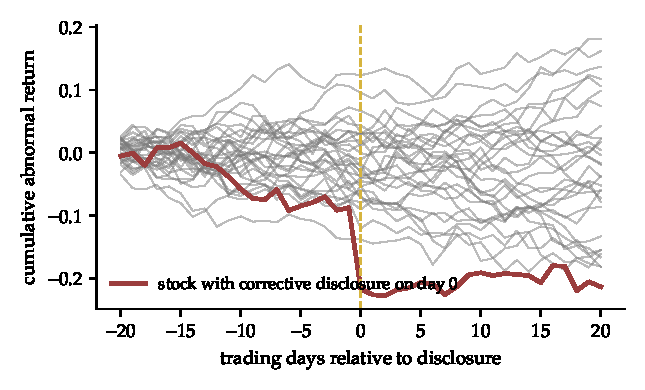
\includegraphics[width=\linewidth]{fig_event}
\caption{Cumulative abnormal returns for a simulated stock with a corrective disclosure on day zero, against thirty simulated paths with no event. Illustrative.}
\label{fig:event}
\end{figure}

\subsection{Problems in court}

Event studies in litigation face well known problems. Single firm, single day tests have low power: a stock with daily volatility of two per cent cannot reliably reveal a price impact of less than about five or six per cent. Volatility changes around news, so the estimation period's $\sigma$ may understate the event day's. Multiple pieces of news on the same day must be disentangled. And the significance threshold, borrowed from academic practice, has no legal warrant: a p value of five per cent is a convention, not a standard of proof. Fisch, Gelbach and Klick have argued that courts misuse significance tests in this context, treating failure to reject the null of no impact as proof of no impact, and treating the five per cent threshold as if it were the civil standard \citep{fox2018}.

\section{A Bayesian event study}

\subsection{From significance to probability}

The legal question in a price impact dispute is whether the misrepresentation or the corrective disclosure moved the price. A Bayesian answer gives the posterior probability that the abnormal return on the event day reflects a genuine price reaction, and the posterior distribution of its size. Let $\delta$ be the true price impact. The observed abnormal return is $a_0 = \delta + \epsilon_0$. With a prior on $\delta$ and the normal model for $\epsilon_0$, the posterior follows directly. To obtain a probability that there was any reaction at all, the prior must place positive probability $p$ on $\delta=0$ (no impact) and spread the remaining $1-p$ over nonzero impacts, as in Question 1; under a purely continuous prior the posterior probability of exactly zero impact is itself zero, and the useful summary is instead the posterior probability that $|\delta|$ exceeds a legally material size. The prior should reflect what is known about price reactions to comparable disclosures: most company news days produce small abnormal returns, and a minority produce large ones.

\subsection{Heavy tailed priors}

The shape of the prior matters. A normal prior shrinks every estimate toward zero by the same proportion, so a large observed abnormal return is shrunk as much, proportionally, as a small one. A heavy tailed prior (a continuous prior, so the question it answers is about the size of the impact), such as a Cauchy or a horseshoe, shrinks small estimates strongly toward zero while leaving large ones nearly untouched \citep{carvalho2010}. Figure~\ref{fig:heavytail} compares the two. For event studies, a heavy tailed prior is a natural modelling choice, since news day returns are mostly small with a few large ones (event day returns are reported to be fat tailed), and it gives answers that match the intuition, given the prior: a large drop on a corrective disclosure day almost certainly reflects a genuine reaction of material size, while a small drop is likely noise.\index{heavy tailed prior}\index{horseshoe prior}

\begin{figure}[t]
\centering
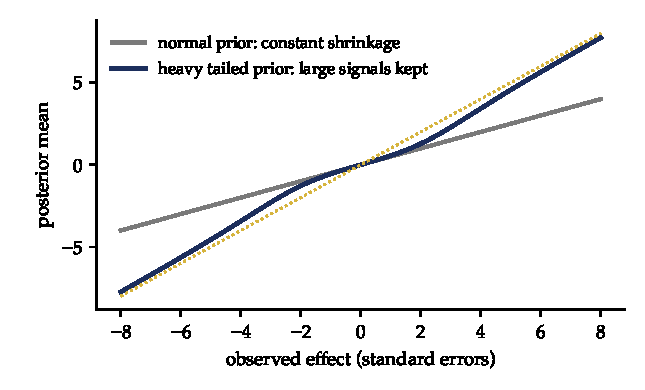
\includegraphics[width=\linewidth]{fig_heavytail}
\caption{Posterior mean of a true effect as a function of the observed effect, under a normal prior and under a heavy tailed (Cauchy) prior, with unit noise. The heavy tailed prior shrinks small observations strongly and large ones hardly at all.}
\label{fig:heavytail}
\end{figure}

Polson and Scott used the same reasoning to screen firms for sustained superior performance, in \emph{Good, great, or lucky?} \citep{polson_scott_lucky}. When many firms are evaluated, most have true excess performance near zero, and a few may be genuinely superior. A heavy tailed prior on performance shrinks the many lucky records toward zero while preserving the few that are too large to be luck. The legal parallels are direct: the same method separates genuine price reactions from noise in event studies, and genuine skill from chance in the games of Chapter~\ref{ch:kadane}.

\subsection{Combining evidence across events}

Price impact often turns on several dates: the original misstatement, partial corrections, and a final disclosure. A hierarchical model treats the impacts on these dates as related, sharing information about the size of the inflation, and estimates them jointly. If the inflation was introduced by a misstatement and removed by several partial disclosures, the impacts should sum, approximately, to the total inflation. This constraint, imposed through the model, strengthens inference about each date. It also addresses the \emph{Goldman} mismatch problem: if a generic statement is alleged to have maintained inflation that a specific disclosure removed, the model must explain why the generic statement carried the specific information, and the prior for that link can be argued about explicitly.

\section{Damages}

Damages in a fraud on the market case are typically measured by the inflation in the price at each purchase date, the difference between the price paid and the price that would have prevailed without the fraud, limited by the decline when the truth emerged. The inflation ribbon, the path of inflation over the class period, is estimated from the event study. Its uncertainty is substantial, and Bayesian methods report it as a posterior distribution rather than a point estimate. In settlement negotiations, which resolve almost all such cases, the posterior distribution of damages, combined with the probability of liability, gives each side's expected value of trial; Chapter~\ref{ch:becker} develops the settlement model that uses it.

\section{Autonomy: Bayes on trial}

\begin{casebox}{ACL Netherlands v Lynch [2022] EWHC 1178 (Ch)}
In 2011 Hewlett Packard acquired Autonomy, a British software company founded by Mike Lynch, for about eleven billion dollars. Autonomy's technology for searching unstructured information was built on Bayesian inference and Shannon's information theory. A year later HP wrote down the value of Autonomy by about nine billion dollars, attributing much of the write down to accounting improprieties. HP's subsidiaries sued Lynch and Autonomy's former finance director in the English High Court under the Financial Services and Markets Act 2000 and in deceit. After a trial that ran from March 2019 to January 2020 and that the judge described as amongst the longest and most complex in English legal history, Mr Justice Hildyard found in 2022 that the defendants had fraudulently inflated Autonomy's reported revenues and that the claimants had succeeded in substantial part \citep{autonomy2022}. Damages were later assessed in a separate judgment at about \pounds 646 million, far below HP's original claim of up to \$5 billion \citep{autonomy2025}. In the United States, Lynch was tried on criminal fraud charges and acquitted by a jury in June 2024. Two months later he died when his yacht, named \emph{Bayesian}, sank off Sicily.
\end{casebox}

\subsection{Different courts, different standards}

The Autonomy litigation shows, like Simpson in Chapter~\ref{ch:classic}, how different standards and procedures can produce different outcomes on overlapping facts. The English civil court applied the balance of probabilities, after a trial in which a single judge heard months of evidence and gave a reasoned judgment of great length. The American criminal jury applied proof beyond reasonable doubt and gave an unreasoned verdict. A posterior probability of fraud somewhere between one half and the criminal threshold would produce exactly these outcomes. The cases also differed in their evidence and in what had to be proved: the English claim under section 90A of the Financial Services and Markets Act turned on the knowledge of persons discharging managerial responsibilities and on the claimants' reliance on published information, while the American prosecution had to prove criminal intent in respect of particular counts.

\subsection{Section 90A and reliance}

Section 90A and Schedule 10A of the Financial Services and Markets Act create liability of an issuer for misleading statements in published information, where a person discharging managerial responsibilities knew the statement was untrue or misleading or was reckless as to that, and the claimant acquired securities in reliance on the information. Unlike American law, English law has not adopted a fraud on the market presumption, and claimants must show reliance on the published information. Claimants in several recent English securities actions have argued that reliance on the market price should suffice, and defendants that individual reliance must be proved. The point is unsettled: in \emph{Allianz Funds v Barclays} the High Court held that reliance under section 90A is the common law deceit test and struck out claims based on reliance on the market price \citep{allianz2024}, but in \emph{Persons Identified in Schedule 1 v Standard Chartered} another High Court judge declined to follow that approach and allowed passive investor claims to go to trial \citep{stanchart2025}. In Bayesian terms, the question is whether the misstatement's effect on the claimant's decision ran through the claimant's own reading of the information, which must be shown individually, or through the price, which can be shown for all buyers at once with an event study. The answer bears on whether securities class actions are viable in England on the American scale, together with the absence of an opt-out regime and the funding and costs rules.

\subsection{The valuation question}

The deeper Bayesian question in Autonomy was what HP would have paid had it known the truth. That is a counterfactual decision, like the insurer's counterfactual premium under the Insurance Act in Chapter~\ref{ch:misrep}. The claimants' loss under the Act was the difference between what they were persuaded to pay and what they would have been persuaded to pay with accurate information, not the whole write down, which also reflected HP's own management of the business after acquisition and changes in market conditions. Separating the effect of the misrepresentation from these other causes required a model of how a buyer values a software company from its revenues, margins and growth, and of how the restated figures would have changed that valuation. The gap between the headline write down and the loss recoverable on this measure illustrates how much of a headline loss can be attributed to causes other than the fraud once the counterfactual is modelled.

\section{Prices as evidence elsewhere}

Market prices are evidence in many other legal contexts. Chapter~\ref{ch:bankruptcy} showed their use in solvency disputes. In appraisal proceedings in Delaware, which determine the fair value of shares of dissenting shareholders in a merger, the Delaware Supreme Court has emphasised the probative value of the deal price when the sale process was sound, and has said that the unaffected market price may be informative in an efficient market but is not necessarily an exclusive indicator \citep{aruba2019}. In antitrust, prices before and during an alleged cartel are compared to estimate overcharges. Prediction market prices are increasingly cited as evidence of expectations. In each case the Bayesian questions are the same: what information does the price aggregate, how reliable is that aggregation, what else moves the price, and how should the price be combined with other evidence?

\section*{Notes and Questions}
\addcontentsline{toc}{section}{Notes and Questions}
\begin{enumerate}[label=\arabic*.]
\item A stock has daily residual volatility of two and a half per cent. On a corrective disclosure date, its abnormal return is minus four per cent. Compute the $t$ statistic. With a prior that ninety per cent of disclosure days have no impact and ten per cent have an impact distributed normally with standard deviation eight per cent, compute the posterior probability of a genuine impact.
\item Explain why a single firm event study has low power, and why failure to find a significant abnormal return does not prove absence of price impact.
\item Compare a normal and a Cauchy prior for a disclosure that produced an abnormal return of ten standard errors. What does each imply about the true impact?
\item In \emph{Goldman}, the alleged misstatements were generic statements about conflicts of interest. Formalise the mismatch argument as a statement about the likelihood that a generic statement carried the information later disclosed.
\item Should English law adopt a fraud on the market presumption for claims under section 90A? Frame your answer in terms of the cost of proving individual reliance and the accuracy of price based inference.
\item Why might a civil court find fraud on the balance of probabilities and a criminal jury acquit on overlapping facts? Use the Autonomy litigation to illustrate.
\end{enumerate}

\section*{Further reading}
The Supreme Court's decisions in \emph{Basic}, \emph{Halliburton} and \emph{Goldman} \citep{basic1988,halliburton2014,goldman2021}; Fisch, Gelbach and Klick on event studies in court \citep{fox2018}; Carvalho, Polson and Scott on the horseshoe prior \citep{carvalho2010}; Polson and Scott on screening firms for sustained performance \citep{polson_scott_lucky}.

\chapter{Clusters, Coincidence and Medical Murder Cases}
\label{ch:clusters}

\section{When deaths cluster around a carer}

A recurring kind of criminal case begins with a cluster. On a hospital ward, more patients than usual die or suffer sudden collapses, and colleagues notice that a particular nurse was on duty for many of them. Suspicion grows, a review is commissioned, the police are called, and eventually the nurse is charged with murder. Some such cases have revealed real killers: Beverley Allitt in England in the early 1990s and Harold Shipman, a general practitioner who killed many of his patients, were convicted on overwhelming evidence. Others have produced miscarriages of justice. The Dutch nurse Lucia de Berk was convicted in 2003 of several murders and attempted murders of patients, partly on the strength of a statistical argument about her presence at incidents, and was exonerated in 2010 after the statistical argument and the medical evidence were reexamined.\index{medical murder cases}\index{Lucia de Berk}

These cases are among the most difficult in criminal law, and they are statistical at their core. The fact that a nurse was present at many incidents is evidence only if her presence is more probable under the hypothesis that she caused the incidents than under the hypothesis that they arose naturally. Assessing that likelihood ratio requires understanding how incidents are identified, how shifts are allocated, how often natural clusters occur, and how suspicion itself shapes the data. The Royal Statistical Society's Statistics and the Law Section published a report in 2022 on statistical issues in the investigation of suspected medical misconduct, setting out these problems and recommending safeguards \citep{rss2022}. This chapter draws on that report and on the cases.

\section{The Lucia de Berk case}

\begin{casebox}{The Lucia de Berk case (Netherlands)}
Lucia de Berk was a nurse in The Hague who worked at a children's hospital and, in the period examined, on adult wards of another hospital. After the unexpected death of a child in her care in 2001, hospital staff reviewed earlier incidents and identified a number in which she had been on duty. A statistician, Henk Elffers, whom the court consulted, calculated that the probability of her being present at so many incidents by chance was about one in three hundred and forty two million. She was convicted in 2003 of several murders and attempted murders, and on appeal she was convicted again, on more counts (seven murders and three attempted murders), though the appeal court said it did not rely on the statistics. After campaigning by scientists, including the statistician Richard Gill, and a reexamination of the medical evidence showing that the death that triggered the investigation was likely natural, the case was reopened, and she was acquitted of all charges in 2010.
\end{casebox}

The one in three hundred and forty two million figure illustrates nearly every error discussed in this book. It was a p value, the probability, under a hypothesis of chance, of data at least as extreme as those observed, presented in a way that invited the prosecutor's fallacy. The incidents were identified after suspicion had fallen on her, so incidents during her shifts were more likely to be recorded as suspicious than similar events during others' shifts. The calculation combined data from several wards by multiplying p values, which is not a valid way to combine evidence. And it ignored the base rate: even if the coincidence was unusual, the prior probability that a nurse is a serial killer is small, and many nurses in many hospitals will by chance be present at clusters of deaths. Gill and colleagues' reanalysis, using more defensible methods, found that the evidence of an unusual association was far weaker than claimed \citep{meester2006,gill2018}.

\section{The statistics of clusters}

\subsection{Clusters happen}

Deaths and collapses on a hospital ward are not evenly spread. They come in clusters because illnesses cluster, because admissions vary, and because chance produces clusters. If a hospital has many wards and each ward has many nurses, then in any year some nurse somewhere will be on duty for an unusually large share of a ward's incidents. The probability that a particular nurse, chosen in advance, is present at a given number of incidents may be small, but the probability that some nurse is present at that many is much larger. This is the multiple comparisons problem, sometimes called the Texas sharpshooter fallacy after the marksman who fires at a barn and then draws a target around the bullet holes (Chapter~\ref{ch:fallacies} treats multiple comparisons and the combining of p values among the fallacies).\index{clusters}\index{Texas sharpshooter fallacy}

Let $n$ nurses work on a ward over a period with $k$ incidents, and suppose nurse $i$ works a fraction $f_i$ of the shifts. Under the hypothesis that incidents occur independently of who is on duty, the number of incidents during nurse $i$'s shifts is binomial with parameters $k$ and $f_i$. The probability that the maximum over nurses exceeds a threshold is the relevant chance probability when the nurse was identified because of her count, and when the nurses work similar shares of the shifts it can be up to about $n$ times larger than the probability for a nurse chosen in advance, and larger by orders of magnitude when the search also ranges over wards, hospitals and periods.

\subsection{Selection of incidents}

The second problem is that the incidents themselves are selected. Whether an event is classified as suspicious, as unexpected, or as an incident at all depends on the judgment of clinicians, and once suspicion has fallen on a nurse, events during her shifts are more likely to be reexamined and reclassified. This creates an association between her presence and the recorded incidents even if she did nothing. In Bayesian terms, the likelihood of the data under innocence must include the probability that an innocent nurse's shifts are subjected to closer scrutiny. If the reviewers knew who was on duty when they classified events, the classifications are contaminated, and their likelihood ratio cannot be estimated reliably without blind review.

\subsection{Shift charts}

A common presentation in such cases is a chart showing, for each suspicious event, which staff were on duty, with the accused nurse's presence at every event highlighted. Such charts are visually powerful and statistically misleading if the events were selected with knowledge of who was on duty, or if events when the accused was absent were excluded as not suspicious. A chart that shows only the events attributed to the defendant will by construction show her present at all of them. The relevant evidence is a comparison of the rate of genuinely unexplained events during her shifts with the rate during others', with events classified by reviewers blind to the rota.\index{shift charts}

\section{The Bayesian analysis}

\subsection{Prior}

The prior probability that a given nurse is deliberately harming patients is small. Healthcare serial killers exist, but they are rare relative to the number of healthcare workers. Any sensible analysis starts from a prior of the order of one in tens or hundreds of thousands, adjusted for anything specific known about the nurse before the investigation.

\subsection{Likelihood of the cluster}

The likelihood ratio of the cluster is the probability of observing the association under the hypothesis of deliberate harm divided by its probability under the hypothesis of natural causes, including the selection and multiple comparison effects. Under deliberate harm, a strong association is expected. Under natural causes, the probability of an association as strong as observed, for some nurse, given how the incidents were identified, may be modest rather than tiny. The likelihood ratio may then be in the tens or hundreds rather than in the millions, which against a prior of one in a hundred thousand leaves a low posterior. The cluster is a reason to investigate, not by itself a reason to convict.

\subsection{Medical evidence}

The decisive evidence in these cases is usually medical: evidence that particular events could only have been caused by deliberate acts, such as the administration of a drug that was not prescribed. Such evidence, if reliable, can have a large likelihood ratio, because natural explanations are excluded. But the reliability of medical evidence of deliberate harm depends on the tests used, their error rates, and whether alternative explanations were considered. In the de Berk case, the reexamination of the medical evidence showed that natural explanations had been wrongly excluded. The Bayesian principle is that each item of medical evidence must be assessed with its own likelihood ratio, including the probability of misinterpretation, and that the items should not be assumed independent when the same experts, aware of the suspicion, interpreted them.

\section{Lucy Letby}

Lucy Letby, a neonatal nurse at the Countess of Chester Hospital, was convicted in 2023 of murdering seven babies and attempting to murder others, and in 2024 of a further attempted murder after a retrial. She received whole life orders. The Court of Appeal refused permission to appeal against the 2023 convictions in 2024, and a separate challenge to the 2024 conviction was also refused. The prosecution case included evidence of her presence at the events, medical evidence that some babies had been harmed by air embolism or by the administration of insulin, notes she had written, and other circumstantial evidence. After the trials, a number of clinicians and statisticians publicly questioned aspects of the evidence, and an international panel of neonatal experts, whose findings were submitted by her legal team, concluded that natural causes and deficiencies in care could explain the events. Her lawyers applied to the Criminal Cases Review Commission in February 2025, and the Commission's review was continuing at the time of writing. In January 2026 the Crown Prosecution Service decided not to bring further charges relating to other babies, and that decision was upheld on review.\index{Lucy Letby}

We express no view on whether the convictions are safe; that is for the Commission and, if the case is referred, the Court of Appeal. What a Bayesian analysis can do is identify the questions on which the safety of such convictions turns, and they are those discussed above. Was the association between the nurse's shifts and the events established with incidents classified blind to the rota? What is the likelihood ratio of the medical findings, including the probability of misdiagnosis of air embolism or of insulin administration, given the tests performed? Were the items of medical evidence interpreted independently, or by experts who knew the hypothesis? How should the circumstantial evidence, including the notes, be weighed, given that its likelihood under innocence depends on the psychological state of a person under suspicion? These are questions about likelihood ratios and their dependence, and they can be framed, and in part bounded, by the methods of this book.

\section{Safeguards}

The Royal Statistical Society's report recommended safeguards for investigations of suspected medical misconduct \citep{rss2022}. In summary, and in our own words:
\begin{enumerate}[label=(\roman*)]
\item Investigations should define incidents and classify them before, and independently of, any knowledge of who was on duty.
\item Statistical analyses should account for multiple comparisons and for how the suspect came to be identified.
\item Comparisons should use the rates of incidents per shift for the suspect and for comparable colleagues, with uncertainty, rather than counts of incidents attended.
\item Medical evidence should be reviewed by experts blind to the suspicion where possible, and the possibility of natural causes should be explicitly assessed.
\item Courts should be presented with likelihood ratios for the evidence, not with p values or probabilities of coincidence.
\item Expert statistical evidence should come from qualified statisticians, with independent review.
\end{enumerate}
Each safeguard addresses a source of bias in the likelihood ratio. Together they would make the evidence in such cases more reliable, whichever way it points.

\section{Wrongful convictions more generally}

Medical murder cases are one class of wrongful conviction. Studies of exonerations in the United States, many documented by the National Registry of Exonerations and the Innocence Project, have identified common contributing factors: mistaken eyewitness identification, false confessions, invalid or misleading forensic evidence, unreliable informants and official misconduct. Each factor corresponds to an error in a likelihood ratio: an identification given more weight than its conditions warranted, a confession whose denominator was raised by coercion, a forensic method without established error rates, an informant with motives to lie, evidence suppressed or fabricated. The Bayesian framework does not prevent wrongful convictions, but it identifies where they come from and what kinds of procedural safeguards address each source.

In England, Wales and Northern Ireland, the Criminal Cases Review Commission, established in 1997, investigates possible miscarriages of justice and may refer cases to the Court of Appeal if there is a real possibility that the conviction would not be upheld. A real possibility is a probability judgment about another court's judgment, a posterior about a posterior. The Commission's caseload and the time it takes have been criticised, and the Post Office Horizon cases taken up in Chapter~\ref{ch:lean} showed how slowly the system can respond to systematic error. A Bayesian triage of applications, of the kind Chapter~\ref{ch:india} proposes for India, could help direct the Commission's resources to the cases with the highest probability of error and the highest cost of delay.

\section*{Notes and Questions}
\addcontentsline{toc}{section}{Notes and Questions}
\begin{enumerate}[label=\arabic*.]
\item A ward has twenty nurses who each work five per cent of shifts. Over a year there are twenty incidents. What is the probability that a nurse chosen in advance is on duty for eight or more? What is the probability that some nurse is?
\item Explain why multiplying p values from several wards, as in the de Berk calculation, does not give a valid measure of evidence. What would?
\item Design a blind classification protocol for incidents in an investigation of a suspected healthcare killer.
\item Suppose the prior probability that a nurse is deliberately harming patients is one in fifty thousand, the cluster evidence has likelihood ratio two hundred, and a toxicology finding has likelihood ratio one thousand if reliable (treat the two items as independent, although the chapter warns that they may not be) but a ten per cent chance of being a laboratory or interpretive error. Compute the posterior.
\item The Criminal Cases Review Commission refers a case when there is a real possibility the conviction would not be upheld. Express this as a threshold on a probability. What threshold would you choose, and why?
\item Shift charts are visually compelling. Draft a direction to a jury on how to interpret a shift chart.
\end{enumerate}

\section*{Further reading}
The Royal Statistical Society report on medical misconduct investigations \citep{rss2022}; Gill's work on the de Berk case \citep{meester2006,gill2018}; and, on wrongful convictions generally, the National Registry of Exonerations.

\chapter{Intellectual Property: Surveys, Obviousness and Machines}
\label{ch:ip}

\section{Property in information}

Intellectual property law grants exclusive rights in inventions, creative works, brands and designs. Its central questions are probabilistic. Would a person skilled in the art have found an invention obvious? Are consumers likely to be confused between two marks? How much of a defendant's profit is attributable to the infringing feature? Would the patentee have made the infringer's sales but for the infringement? Each question asks a court to estimate a probability or a counterfactual from imperfect evidence, and each has generated its own statistical methods. And intellectual property is where artificial intelligence presents the law with its most direct questions: can a machine be an inventor, and can a machine learn from protected works without permission? This chapter treats these questions with the tools of the book.\index{intellectual property}

\section{Consumer confusion and surveys}

\subsection{The legal question}

Trade mark infringement in many cases turns on whether there is a likelihood of confusion on the part of the public: whether an average consumer, reasonably well informed and reasonably observant and circumspect, would be likely to believe that goods bearing the defendant's sign come from the claimant or a connected undertaking. In the United States, the Lanham Act asks whether a use is likely to cause confusion. Likelihood is a probability, and courts in both systems have used consumer surveys as evidence of it.\index{trade marks}\index{consumer confusion}

\subsection{Surveys as evidence}

A confusion survey\index{survey evidence} shows respondents the defendant's product and asks questions designed to reveal whether they associate it with the claimant. The proportion who do is compared with the proportion in a control group shown a product that differs in the allegedly infringing feature. The difference estimates the confusion caused by the feature. Survey design matters greatly: leading questions, unrepresentative samples and inappropriate controls can produce any result the sponsor wants. English courts have been sceptical of surveys, and in \emph{Interflora v Marks and Spencer} the Court of Appeal emphasised that permission to adduce survey evidence should be given only where the evidence is likely to be of real value and its cost justified \citep{interflora2012,interflora2013}. American courts admit surveys more readily and weigh their methodological quality.

In Bayesian terms, a survey is an estimate of a population proportion with sampling error and possible bias. The legal question is not whether the proportion exceeds zero but whether it exceeds a threshold that would make confusion likely in the relevant sense, a threshold courts have rarely stated. A Bayesian analysis reports the posterior distribution of the net confusion rate, after subtracting the control, with priors on bias informed by the survey's design, and asks the court what level of confusion matters. Stating the threshold, even approximately, would make survey evidence more useful and decisions more consistent.

\section{Obviousness}

\subsection{The test}

A patent is invalid if the invention was obvious to a person skilled in the art at the priority date, having regard to the state of the art. UK courts apply a structured approach, following \emph{Pozzoli v BDMO}, asking what the skilled person would have known, what the inventive concept is, what the differences are between the prior art and the invention, and whether those differences would have been obvious steps \citep{pozzoli2007}. American courts apply \emph{Graham v John Deere} and, since \emph{KSR v Teleflex}, a flexible test that asks whether a person of ordinary skill would have had reason to combine prior art elements with a reasonable expectation of success \citep{ksr2007}.\index{obviousness}

\subsection{A probabilistic reading}

Obviousness has a natural probabilistic reading: an invention is obvious if a skilled person, starting from the prior art, would have arrived at it with high probability without inventive effort. The phrase reasonable expectation of success, which the Federal Circuit applies alongside \emph{KSR}, is explicitly probabilistic. Courts sometimes speak of an invention being obvious to try, where there were a finite number of identified, predictable solutions; that corresponds to a high probability that routine experimentation would find the answer.

The difficulty is hindsight, the same difficulty as in Chapter~\ref{ch:bankruptcy}. Once an invention is known, the path to it looks obvious. Courts warn against hindsight, but the warning is hard to follow. Secondary considerations, such as long felt need, the failure of others and commercial success, are evidence about the ex ante probability that a skilled person would have found the invention: if many skilled people tried and failed, the probability was low. A Bayesian court treats them as likelihood ratios for the hypothesis that the invention was obvious, weighing them against the expert's reconstruction of the path from prior art, which is vulnerable to hindsight bias.

\section{Damages in patent cases}

\subsection{Lost profits}

A patentee can recover the profits it would have made but for the infringement. In the United States the \emph{Panduit} factors ask about demand for the product, the absence of acceptable non infringing substitutes, the patentee's capacity, and the amount of profit. Each is an input to a counterfactual: what sales the patentee would have made had the infringer been absent. The counterfactual requires a model of demand and substitution, of the kind Chapter~\ref{ch:antitrust} discusses later for merger simulation, and its answer is uncertain. A Bayesian assessment produces a posterior distribution for lost profits, and the award should, by default, be its mean, for the reasons given in Chapter~\ref{ch:damages}.

\subsection{Reasonable royalties}

Where lost profits cannot be shown, the patentee recovers a reasonable royalty\index{reasonable royalty}, often assessed by a hypothetical negotiation between a willing licensor and a willing licensee at the time infringement began, considering factors listed in \emph{Georgia Pacific}. The hypothetical negotiation is the counterfactual bargaining problem of negotiating damages in Chapter~\ref{ch:damages}. Comparable licences provide evidence, as do the infringer's expected profits from using the invention. The apportionment problem, how much of a product's value is due to the patented feature among many, has been a central issue in cases involving complex products with thousands of patents. Apportionment is a causal question: what is the marginal contribution of the feature to demand? Conjoint surveys, which estimate consumers' valuation of features from their choices among hypothetical products, are increasingly used to answer it, with the strengths and weaknesses of all survey evidence.

\section{Machines as inventors}

\subsection{DABUS}

Stephen Thaler filed patent applications in several countries naming as inventor an AI system he had built, called DABUS, and claiming the right to the patents as its owner. The applications were refused in the United Kingdom, the United States, the European Patent Office and elsewhere. South Africa granted a patent in 2021 without substantive examination, and an Australian judge at first instance allowed the application in 2021, but the Full Federal Court reversed that decision in 2022. In \emph{Thaler v Comptroller General of Patents} the UK Supreme Court held in 2023 that an inventor under the Patents Act 1977 must be a natural person, so that DABUS could not be an inventor, and that Thaler was not entitled to the patents merely by owning the machine \citep{thaler2023}. The American Federal Circuit had reached a similar conclusion in \emph{Thaler v Vidal}.\index{DABUS}\index{AI inventorship}

The decisions leave open the more practical question: what happens when a human uses an AI system to help make an invention? The United States Patent and Trademark Office's revised guidance of November 2025 treats an AI system as a tool: only natural persons can be inventors, and a human who conceives the invention under the ordinary conception standard is the inventor even if AI assisted \citep{uspto2025}. Whether the human conceived the invention can be read as a question about the counterfactual: would the invention have been made without the human? In a world where AI systems can generate candidate inventions in large numbers, the obviousness standard itself may shift: if a skilled person equipped with standard AI tools would have found the invention with high probability, it is obvious. The person skilled in the art, a legal fiction, may soon be a person with a machine.

\section{Machines learning from works}

Generative AI systems are trained on large collections of text, images and other works, many protected by copyright. Whether such training infringes copyright, and whether the outputs infringe, are being litigated in several jurisdictions. The issues include whether training involves copying, whether any copying is excused by fair use in the United States or by text and data mining exceptions in the European Union and the United Kingdom, whether outputs reproduce protected expression, and how damages should be measured. Several cases have settled, some for large sums: the class claim against Anthropic over pirated copies of books it downloaded to build a training library settled for \$1.5 billion, with final approval granted in July 2026, after the court had held that training on the books was itself fair use \citep{bartz2026}. Others continue.

The Bayesian contribution to these disputes is evidential and remedial. Whether a model's output reproduces a protected work is a question with a likelihood ratio: how probable is the similarity if the model memorised the work, against the probability of similarity arising independently from the general distribution of works? The second probability is the analogue of the random match probability in Chapter~\ref{ch:odds}, and it can be estimated by comparing outputs with many works. Damages, if liability is found, raise the apportionment problem again: how much of a model's value derives from any particular work in a training set of billions? The answer is small for most works and the method of estimation, perhaps by the marginal contribution of a work or a class of works to model performance, is an open research problem with legal consequences.

\section*{Notes and Questions}
\addcontentsline{toc}{section}{Notes and Questions}
\begin{enumerate}[label=\arabic*.]
\item A confusion survey finds that twenty two per cent of the test group and eight per cent of the control group associate the defendant's product with the claimant, with samples of two hundred each. Compute the posterior distribution of the net confusion rate. What threshold would you propose for likely confusion?
\item Explain why secondary considerations such as the failure of others are evidence about obviousness. Express each as a likelihood ratio.
\item In a hypothetical negotiation, the patentee's minimum royalty is two per cent of sales and the infringer's maximum is six per cent. What royalty would a court award? How should uncertainty about these bounds affect the award?
\item Should a person skilled in the art be assumed to use AI tools? How would that change the obviousness of inventions in a field where AI design tools are standard?
\item Propose a method for estimating the contribution of a single work to the value of a generative model trained on billions of works.
\end{enumerate}

\section*{Further reading}
\emph{KSR v Teleflex} \citep{ksr2007}; \emph{Thaler v Comptroller} \citep{thaler2023}; \emph{Interflora v Marks and Spencer} on survey evidence \citep{interflora2012,interflora2013}.

\chapter{Digital Evidence, Surveillance and Privacy}
\label{ch:digital}

\section{Evidence at scale}

Much evidence in modern litigation is digital. Emails, messages, location records, financial transactions, social media posts, video from cameras, logs from devices: the record of a person's life is now largely kept by machines. Investigators search it with tools that operate at scale, matching faces against databases of millions, collecting the identities of every phone near a crime scene, scanning communications for keywords. Each tool produces signals with error rates, and because they operate at scale, small error rates produce large numbers of false matches. This chapter applies the base rate reasoning of Chapters~\ref{ch:odds} and~\ref{ch:classic} to digital evidence and surveillance, and examines how the law of privacy constrains the information available to courts.\index{digital evidence}

\section{Facial recognition}

\subsection{Matching at scale}

Automated facial recognition compares a probe image, such as a still from a camera, with a database of known faces and returns candidate matches above a similarity threshold. Its accuracy has improved greatly, but every system has a false match rate: the probability that an image of one person is matched to another. When the probe is compared with a database of $N$ people, the expected number of false matches is approximately $N$ times the false match rate. With a database of ten million and a false match rate of one in a million, ten false candidates are expected for every search, in addition to the true match if the person is in the database.\index{facial recognition}\index{Bridges, R v Chief Constable of South Wales Police}

This is the island problem in its purest form. The posterior probability that a returned candidate is the person in the probe image depends on whether the person is in the database at all, the prior, and on the number of false candidates, which grows with the database. A candidate returned by a search of a large database, with no other evidence, has a modest posterior probability of being the right person, however impressive the similarity score. Several wrongful arrests in the United States have followed facial recognition matches treated as identifications rather than as leads. The Bayesian lesson is that a match from a large database search is a reason to investigate, with a likelihood ratio that must be combined with a prior, not an identification.

\subsection{Live deployment and the law}

In \emph{R (Bridges) v Chief Constable of South Wales Police} the Court of Appeal held in 2020 that the police's use of live automated facial recognition in public places was unlawful, not as a blanket ban but because the interference was not in accordance with the law, since the legal framework left too much discretion to individual officers about who could be placed on watch lists and where the technology could be deployed, because the data protection impact assessment was deficient, and because the force had not taken reasonable steps to satisfy itself that the software did not have an unacceptable bias on grounds of race or sex \citep{bridges2020}. The last point is a requirement to measure error rates by group, the analysis of error rates by group in Chapter~\ref{ch:lindleyai}. A system whose false match rate is higher for some groups produces more false stops of members of those groups, a disproportionate effect that the public sector equality duty requires the authority to investigate. The court did not find the interference disproportionate.

\section{Location data}

\subsection{Cell site records}

Mobile phones register with nearby cell towers, and network operators keep records of which towers a phone used and when. These records place a phone, approximately, at a location at a time. In \emph{Carpenter v United States} the Supreme Court held in 2018 that acquiring historical cell site location information covering a substantial period is a search under the Fourth Amendment, generally requiring a warrant \citep{carpenter2018}. The Court reasoned that such records provide an intimate window into a person's life, revealing not only movements but associations.\index{location data}\index{Carpenter v United States}

\subsection{What location evidence proves}

Location records are evidence of the phone's location, not the person's. The likelihood ratio of a record placing the defendant's phone near a crime scene depends on how precise the location is, how many other phones were in the same area, how probable it is that the defendant's phone would be there for innocent reasons, and how probable it is that someone else had the phone. A tower that serves a dense urban area covers thousands of people; one in a rural area may cover few. A record that places a phone in a large sector of a city at a time when the defendant lived there has a likelihood ratio close to one. One that places it at a remote location where the defendant had no reason to be may have a large likelihood ratio. Experts who present location evidence must explain these factors, and courts should be wary of maps that display coverage areas as points.

\subsection{Geofence warrants}

A geofence\index{geofence warrants} warrant asks a provider to identify all devices present in a defined area during a defined time. It reverses the usual order of investigation: instead of identifying a suspect and then seeking his location, it collects everyone present and then narrows down. Courts in the United States have divided on whether such warrants are constitutional. The Bayesian analysis is the database search of Chapter~\ref{ch:classic}: everyone in the geofence is a candidate, the prior for each is roughly one over the number of people who could have committed the crime, before the geofence results are seen, and further evidence must do the work of identifying the offender. The constitutional concern is about the privacy of the many innocent people swept up; the evidential concern is that a person identified only by presence in a geofence has a low posterior probability of guilt.

\section{Communications and keyword searches}

Investigators and litigants search large collections of communications for relevant material, using keywords, technology assisted review and, increasingly, language models. Chapter~\ref{ch:lindleyai} discusses the acceptance of technology assisted review in disclosure. In criminal investigations, the failure to disclose relevant material found in digital records has led to prosecutions collapsing. In England, the rape trial of Liam Allan collapsed at Croydon Crown Court in December 2017, when messages on the complainant's phone that undermined the prosecution case came to light after not being disclosed; a joint review by the Metropolitan Police and the Crown Prosecution Service attributed the failure to a combination of error, lack of challenge, and lack of knowledge \citep{metcps2018}. The problem is partly one of volume, since a single phone may hold hundreds of thousands of messages, and partly one of incentives. A disclosure process is a search with recall and precision, and its error rates should be measured: what fraction of relevant material does the process find, and what fraction of what it finds is relevant? A process with low recall fails defendants.

\section{Authentication}

Digital evidence can be altered, and generative AI now makes fabrication easy, as Chapter~\ref{ch:lindleyai} discusses. Courts have long required evidence to be authenticated, that is shown to be what it purports to be. For digital evidence, authentication\index{authentication} involves metadata, chains of custody, hash values that detect alteration, and expert examination. The likelihood ratio of a digital record for the fact it records is bounded by the reciprocal of the probability that such a record would exist, fabricated or altered, if the fact it records were false. As fabrication becomes cheaper, that probability rises for evidence whose provenance is not established, and the evidential value of unauthenticated recordings falls. Cryptographic provenance standards, which sign content at the point of capture, offer a way to restore it. Courts may come to distinguish sharply between evidence with verifiable provenance and evidence without.

\section{Privacy as a constraint on evidence}

Privacy law limits the information available to courts and investigators. Data protection law in the United Kingdom and the European Union governs the processing of personal data, including by law enforcement, and requires that processing be necessary and proportionate. Constitutional protections, such as the Fourth Amendment in the United States and Article 8 of the European Convention on Human Rights, limit searches and surveillance. These limits have costs in lost evidence, which a decision theoretic analysis can estimate as the expected increase in decision loss from excluding the information, and benefits in protecting the privacy of the many people whose data would otherwise be collected, most of whom have done nothing wrong.

The scale of digital surveillance changes the balance. A tool that searches the data of millions to find one offender imposes a privacy cost on millions and produces many false candidates. The base rate argument and the privacy argument point the same way: mass searches produce low posterior probabilities for the individuals they flag and large intrusions on everyone. Targeted searches, based on prior evidence that raises the probability for a particular person, produce higher posterior probabilities and smaller intrusions. The requirement of individualised suspicion, which runs through the law of search and seizure, is in Bayesian terms a requirement that the prior be raised by evidence specific to the person before the search, not after.

\section*{Notes and Questions}
\addcontentsline{toc}{section}{Notes and Questions}
\begin{enumerate}[label=\arabic*.]
\item A facial recognition system with a false match rate of one in a million searches a database of twelve million. The person in the probe image is in the database with probability one half, and if so the true match is always returned. If the system returns one candidate above threshold, what is the probability that the candidate is the person in the image?
\item A cell site record places the defendant's phone in a sector covering forty thousand residents at the time of a crime. The defendant lives in the sector. Estimate the likelihood ratio of the record for the hypothesis that the defendant committed the crime.
\item Explain why a geofence warrant is a database search in the sense of Chapter~\ref{ch:classic}. What is the prior for each device identified?
\item A disclosure process for a phone with two hundred thousand messages has recall of seventy per cent. If ten messages would undermine the prosecution case, what is the probability that at least one is missed? Assume each message is found independently with probability seven tenths.
\item Express the requirement of individualised suspicion as a condition on the prior before a search. Why does it protect both privacy and the accuracy of evidence?
\end{enumerate}

\section*{Further reading}
\emph{Carpenter v United States} \citep{carpenter2018}; \emph{R (Bridges) v Chief Constable of South Wales Police} \citep{bridges2020}.


\part{Comparative Law}
\chapter{Common Law and Civil Law: England and France}
\label{ch:commoncivil}

\begin{quote}\itshape
By law is meant the tendency of a series to repeat itself.
\par\hfill\normalfont Swami Vivekananda, \emph{Karma Yoga}
\end{quote}

\section{Two traditions}

The legal systems of the modern world descend mainly from two traditions. The common law grew in England from the decisions of royal judges after the Norman conquest, developed through precedent and the jury, and spread with the British Empire to the United States, India, much of Africa, Australia and elsewhere. The civil law descends from Roman law as revived in the medieval universities, was codified in France under Napoleon and in Germany at the end of the nineteenth century, and spread through conquest, colonisation and imitation to continental Europe, Latin America, much of Africa and the Middle East, and parts of Asia. The two traditions differ in their sources of law, the role of judges, the procedure of trials and the treatment of evidence. Comparative lawyers have long debated how deep these differences go. Economists, as Chapter~\ref{ch:llsv} discusses, have argued that they matter for financial development and growth.\index{common law}\index{civil law}

This chapter compares English and French law through a Bayesian lens. We ask how each system acquires information about facts, how it aggregates information about law across cases, and how it decides under uncertainty. The comparison is not meant to rank the systems, each of which has strengths, but to show that their differences can be understood as different solutions to the same inference and decision problems.

\section{Sources of law: precedent and code}

\subsection{Stare decisis}

In the common law, the decisions of higher courts bind lower courts, and courts generally follow their own earlier decisions. The binding part of a decision is its ratio decidendi, the principle necessary to the result; other statements are obiter dicta. A court faced with a precedent can follow it, or distinguish it by finding a material difference in the facts. The House of Lords in its 1966 Practice Statement announced that it would depart from its own previous decisions when it appeared right to do so, a power the Supreme Court inherited.\index{stare decisis}

\subsection{The code}

In the French tradition, the primary source of law is legislation, above all the codes. Article 5 of the Code civil forbids judges to pronounce by way of general and regulatory disposition on the cases submitted to them; a judgment decides the dispute between the parties and does not make law for others. The Revolution's distrust of the old \emph{parlements}, which had used their judicial power to resist royal reform, shaped this rule. In practice, the decisions of the Cour de cassation are followed by lower courts, and a consistent line of decisions, \emph{jurisprudence constante}, carries great authority. But the theory is that the code is the law, and judges apply it.\index{Code civil}\index{Cour de cassation}

\subsection{A Bayesian reading}

Think of the law on a given question as an unknown function $f$ mapping facts to legal consequences. A legal system is a procedure for estimating $f$ and applying the estimate to new cases. In the civil law, the legislature supplies an explicit specification of $f$ in the code, a strong prior, and courts apply it, refining its interpretation as cases arise. In the common law, $f$ is learned from cases: each decision is a data point, and the body of precedent is the posterior. Distinguishing a precedent is adding a covariate: the court finds that the earlier decision applies to a region of fact space different from the present case.

A hierarchical model captures both systems. Let $\beta_c$ denote the rule applied in case $c$, and suppose
\begin{equation}
\beta_c = \beta_0 + \eta_{g(c)} + \epsilon_c,
\end{equation}
where $\beta_0$ is a general principle, $\eta_g$ is a refinement for a category $g$ of cases, and $\epsilon_c$ is case specific variation. In a code system, $\beta_0$ and many $\eta_g$ are fixed by legislation with small prior variance; courts estimate the residual variation. In a precedent system, $\beta_0$ is weakly specified, and the $\eta_g$ are learned from the decisions in each category, with shrinkage toward $\beta_0$ that depends on how many cases have been decided. New categories, where few cases exist, are close to the general principle; mature categories have their own well estimated rules.

This reading explains familiar features of both systems. Codes are clear and predictable in their core but can be slow to adapt to new circumstances, since changing the prior requires legislation. Precedent adapts to new facts case by case but can be unpredictable in new areas and can accumulate inconsistent decisions that must be reconciled. Gennaioli and Shleifer modelled the evolution of the common law as a process in which judges distinguish precedents to reach preferred outcomes, and showed that this can make the law more refined over time even when judges are biased \citep{gennaioli2007}. Earlier, Priest and Rubin had argued that the common law tends toward efficiency because inefficient rules are litigated more often and so are more often overturned \citep{priest1977,rubin1977}. Each of these is a theory of how a learning process converges, or fails to.

\section{Procedure: adversarial and inquisitorial}

\subsection{The English trial}

In the English trial the parties control the case. They decide which issues to raise, which witnesses to call and which documents to disclose, subject to rules of disclosure. The judge is an umpire who rules on admissibility and directs the jury on the law. Witnesses are examined orally and cross examined by the opposing party. In Crown Court trials the jury decides the facts and gives a general verdict without reasons. In civil trials the judge almost always decides alone and gives reasons.\index{adversarial procedure}

\subsection{The French trial}

In French criminal procedure a serious case is investigated by a \emph{juge d'instruction}, an examining magistrate, who gathers evidence for and against the accused and compiles a written dossier. The trial court, for the most serious crimes the \emph{cour d'assises} composed of professional judges and lay jurors, has the dossier before it. The presiding judge questions the accused and witnesses; the prosecutor and counsel may put questions directly with the president's leave, and the accused and the civil party may put questions through the president. Written evidence plays a larger role than in England. In civil procedure, the judge has wider powers to order measures of investigation, and oral testimony is less central.\index{inquisitorial procedure}\index{juge d'instruction}

\subsection{Information acquisition}

A Bayesian model of procedure asks how each system acquires and aggregates information. In the adversarial system there are two information gatherers, each with an incentive to find evidence favourable to its side and to present it persuasively. The fact finder hears two selected samples. Dewatripont and Tirole showed that advocacy can produce more information than a single neutral investigator, because each advocate has strong incentives to search for evidence on its side, and the competition between them ensures that both sides are explored \citep{dewatripont1999}. The cost is that each side presents only favourable evidence, so the fact finder must discount for selection, and unfavourable evidence may never be found if neither side has an incentive to seek it.

In the inquisitorial system there is one information gatherer, who is supposed to be neutral. If the investigator is genuinely neutral and well resourced, the sample is unbiased. If the investigator forms a hypothesis early and seeks confirming evidence, a pattern documented in the psychology of investigation, the sample is biased toward that hypothesis and there is no opposing advocate to correct it. The Kercher case of Chapter~\ref{ch:stories}, tried under Italy's mixed system, shows how a theory adopted early in an investigation can shape the evidence collected.

Suppose each item of evidence is a signal with likelihood ratio $\lambda_k$. An unbiased investigator collects items at random; their expected log likelihood ratio is the Kullback Leibler divergence between the distributions under the true and false hypotheses, positive under the true one. An advocate collects items selectively: from a pool of $n$ available items it presents those with $\lambda_k$ favourable to its side. If both advocates search the same pool, the fact finder sees both tails, and the sum of log likelihood ratios across both presentations has, when the log likelihood ratios are symmetrically distributed, an expected value proportional to the total log likelihood ratio of the pool (with $m$ items presented by each side from a pool of $n$, it is $2m/n$ times the expected total), though it is noisy and the proportionality fails for skewed pools. If one side has more resources, it searches more of the pool, and the sum is biased toward it. The adversarial system thus works best when the parties are evenly matched, which is a Bayesian argument for legal aid and for equality of arms.

\section{Evidence and the standard of proof}

\subsection{Free proof and inner conviction}

French criminal law follows the principle of free proof: offences may be proved by any mode of proof, and the judge decides according to his inner conviction. Article 353 of the Code de proc\'edure p\'enale states that the law does not ask judges to account for the means by which they were convinced, and does not prescribe rules by which they must assess the fullness and sufficiency of a proof; it asks them only whether they have an inner conviction, the \emph{intime conviction}. The formula, read aloud to the \emph{cour d'assises} before deliberation, is a statement in the spirit of subjective Bayesianism: the court's posterior is what matters, and no rule fixes how it must be formed.\index{intime conviction}

Until 2012, the \emph{cour d'assises} gave no reasons for its verdicts, like an English jury. After the European Court of Human Rights held in \emph{Taxquet v Belgium} that, although jurors need not give reasons, the accused must be able to understand why he was convicted, which requires procedural safeguards such as precise questions put to the jury \citep{taxquet2010}, France required the \emph{cour d'assises} to state the main elements that convinced it, in a reasoned statement annexed to the verdict. England has not followed: the jury's verdict remains unreasoned, and the Court of Appeal reviews the safety of convictions on the evidence and the judge's directions.

\subsection{Written evidence in civil cases}

French civil law requires written proof for juridical acts above a modest threshold, now set by decree at fifteen hundred euros: a contract above that value must in principle be proved by a written instrument, and oral testimony cannot contradict a written instrument. English law has no general rule of this kind, although some contracts, such as those for the sale of land, must be in writing. The French rule is a prior on the reliability of evidence types: written evidence is presumed more reliable than oral testimony, and the law fixes the weight in advance rather than leaving it to the judge. In Bayesian terms it imposes a likelihood ratio of one on oral evidence contradicting a writing, so that such evidence cannot move the posterior, a strong form of regularisation.

\subsection{Standards of proof}

The English civil standard, the balance of probabilities, has no exact French counterpart. French civil judges are said to decide on their conviction, and French scholars debate whether a standard more demanding than preponderance applies. Empirical comparisons are difficult because French judgments are short and do not usually state the degree of belief reached. Kevin Clermont and Emily Sherwin argued that civil law systems apply a higher civil standard, close to the criminal one, and that the high standard conveys an impression of accuracy and certainty that boosts the legitimacy of decisions \citep{clermont2002}. If they are right, the French system implies a ratio of losses in civil cases that favours defendants, and the English one treats the parties symmetrically.

\section{Loss of a chance in France}

Chapter~\ref{ch:tort} discussed the English refusal, in \emph{Gregg v Scott}, to award damages for loss of a chance of recovery in clinical negligence. French law takes the opposite view. Since the 1960s the Cour de cassation has accepted that a patient whose chance of recovery or survival was reduced by a doctor's fault may recover for the lost chance, with damages equal to a fraction of the loss corresponding to the probability lost. The doctrine of \emph{perte de chance} is applied across many fields: a candidate deprived of the chance to sit an examination, a litigant whose lawyer missed a deadline, a patient whose diagnosis was delayed.\index{perte de chance}

The French approach is the proportional rule that expected utility recommends and that our tort paper defends \citep{polson_sokolov_tort}. Its adoption in France and rejection in England is instructive. It suggests that the English majority in \emph{Gregg} was not compelled by the logic of tort law, since another developed legal system reached the opposite result, but made a policy choice, one that we argued in Chapter~\ref{ch:tort} produces worse incentives and less accurate compensation.

\section{Tort: general clause and strict liability}

The French law of delict rests on general clauses. Article 1240 of the Code civil, formerly Article 1382, provides that any act whatever of man which causes damage to another obliges the one by whose fault it occurred to compensate it. Article 1242, formerly Article 1384, makes a person liable for damage caused by things in his custody. In the \emph{Jand'heur} decision of 1930 the Cour de cassation interpreted this provision as establishing a presumption of liability for damage caused by things, rebuttable only by proof of an external cause, which became a general regime of strict liability for things. The Badinter law of 1985 created a special regime of near strict liability for road traffic accidents, under which victims other than drivers recover except in narrow cases of their own inexcusable fault.\index{Jand'heur}\index{Loi Badinter}

English law has no general clause. It recognises specific torts, of which negligence is the most general, and strict liability is exceptional, as in \emph{Rylands v Fletcher}. In decision terms, the French regime places more of the expected cost of accidents on those who control dangerous things, and so gives them incentives both to take due care and to moderate their activity levels, as Shavell's analysis predicts \citep{shavell1987}. The English regime requires the claimant to prove fault, which reduces liability costs for defendants and raises the cost of proving claims.

\section{Machines and judges in France}

France has taken a distinctive position on the use of data about judges. Article 33 of the 2019 law reforming the justice system (Loi no 2019-222 of 23 March 2019, \emph{Journal officiel} no 0071 of 24 March 2019), the open data provision on court decisions, prohibits the reuse of the identity data of magistrates and court clerks for the purpose of evaluating, analysing, comparing or predicting their actual or alleged professional practices, on pain of criminal penalties. The provision was a response to commercial products that analysed judges' decisions to predict outcomes, and to concern that such analysis would encourage forum shopping and pressure on individual judges.\index{judicial analytics}

The French ban reflects a view that judges should be seen as applying the law, not as individuals with predictable tendencies, a view rooted in Article 5 of the Code civil. The common law tradition, in which individual judges write signed opinions and are known by their reasoning, takes a different view, and judge level analytics are lawful and widely sold in the United States. A Bayesian perspective would note that the information exists whether or not it is analysed: parties and their lawyers form beliefs about judges in any case. The question is whether formal analysis makes those beliefs more accurate, and whether accuracy about judges is desirable. If outcomes depend heavily on which judge hears a case, that is a defect in the system, and analysis that reveals it is valuable for reform. If outcomes depend little on the judge, analysis will reveal that too.

At the same time, France has been a leader in the formal representation of law. The Catala programming language, developed by researchers at Inria, has been used to encode US tax rules on the sale of a principal residence and French family benefits rules, so that the computation of entitlements can be checked against the text \citep{merigoux2021}. Chapter~\ref{ch:lean} discusses this work. It fits naturally with a code based system, in which the law is a text that can be translated into another formal language.

\section{Convergence}

The two traditions have moved toward each other. English civil procedure, after the Woolf reforms (the Civil Procedure Rules 1998, in force from 1999), gives judges active case management powers that resemble the inquisitorial model. The Civil Procedure Rules encourage single joint experts. Statutes now govern large areas of English law once left to the common law. French courts have become more open about their reasoning, the Cour de cassation has reformed the drafting of its judgments to give fuller reasons, and the European courts have imposed common standards on both systems. Mixed jurisdictions such as Scotland, Quebec, Louisiana and South Africa combine features of both. Cameroon, as Chapter~\ref{ch:africa} discusses, contains both within one state.

The Bayesian reading suggests why convergence is natural. Both systems face the same inference problems, and each has learned from the other's solutions. Precedent systems have adopted codes where predictability matters, and code systems have accepted the authority of consistent case law where codes are silent. Adversarial systems have added neutral experts to reduce selection bias, and inquisitorial systems have strengthened the rights of the defence to reduce confirmation bias. The optimal procedure, in a given context, depends on the costs of information, the incentives of the participants and the losses from error, not on tradition.

\section*{Notes and Questions}
\addcontentsline{toc}{section}{Notes and Questions}
\begin{enumerate}[label=\arabic*.]
\item In the hierarchical model of this chapter, suppose $\beta_0$, $\sigma^2$ and $\tau^2$ are known, $\beta_c \sim N(\beta_0 + \eta_g, \sigma^2)$ for a case in category $g$, and $\eta_g \sim N(0,\tau^2)$. After $n_g$ decided cases in category $g$, what is the posterior mean of $\eta_g$? Interpret the shrinkage factor as the weight of precedent.
\item In the adversarial information model, suppose a pool of twenty items has log likelihood ratios drawn from $N(0.5, 1)$ under the true hypothesis. Each advocate presents the five items most favourable to its side. Compute by simulation the expected sum of presented log likelihood ratios and compare it with the expected total for the pool. What happens if one advocate can search only half the pool?
\item Compare the reasons given by a French \emph{cour d'assises} since 2012 with the directions given to an English jury. Which provides more information about the court's posterior?
\item Read the speeches in \emph{Gregg v Scott} and a French decision on \emph{perte de chance}. Is the difference in outcome principled?
\item Should England follow France in prohibiting analytics about individual judges? Frame your answer in terms of the value of information to litigants and to reformers.
\item Explain the French rule requiring written proof of contracts above a threshold as a choice of prior. What are its costs?
\end{enumerate}

\section*{Further reading}
Zweigert and K\"otz's \emph{Introduction to Comparative Law} is the standard text \citep{zweigert1998}. Dewatripont and Tirole on advocates \citep{dewatripont1999}; Gennaioli and Shleifer on the evolution of the common law \citep{gennaioli2007}; Clermont and Sherwin on standards of proof \citep{clermont2002}.

\chapter{Legal Origins and Finance}
\label{ch:llsv}

\section{Law and finance}

In 1997 and 1998 Rafael La Porta, Florencio L\'opez-de-Silanes, Andrei Shleifer and Robert Vishny published two papers that changed how economists think about law \citep{llsv1997,llsv1998}. Robert Vishny, a colleague at Chicago Booth, and his coauthors asked a simple question: do the legal rules that protect outside investors differ across countries, and if so, do the differences explain why some countries have large capital markets and dispersed ownership while others have small markets and concentrated ownership? Their answer was yes, and the differences were organised by legal origin. Countries whose commercial law descends from English common law protected shareholders and creditors more strongly than those whose law descends from French civil law, with German and Scandinavian civil law countries in between. Strong protection was associated with larger equity markets, more initial public offerings and more dispersed ownership.\index{La Porta, L\'opez-de-Silanes, Shleifer and Vishny}\index{legal origins}

The papers launched a literature of thousands of articles, influenced the World Bank's \emph{Doing Business} reports, and provoked fierce criticism. This chapter explains what the authors found, how they measured it, what the critics said, and how a Bayesian approach to the evidence clarifies what we can and cannot conclude.

\section{Measuring investor protection}

\subsection{The antidirector rights index}

\emph{Law and Finance} coded the company and bankruptcy laws of forty-nine countries. For shareholders, the authors constructed an antidirector rights index by adding one point for each of six provisions that strengthen minority shareholders against managers and controlling shareholders: shareholders can vote by mail; shares are not blocked before a shareholders' meeting; cumulative voting or proportional representation of minorities on the board is allowed; there is a legal mechanism for oppressed minorities to challenge directors' decisions; shareholders have pre-emptive rights to new issues; and the share of capital needed to call an extraordinary meeting is ten per cent or less. The index ranges from zero to six. Common law countries averaged about four, French civil law countries about two and a third.\index{antidirector rights index}

\subsection{Creditor rights}

For creditors, the index added one point for each of four provisions: restrictions on entering reorganisation, such as creditor consent; no automatic stay on secured assets; secured creditors paid first in liquidation; and management does not stay in control during reorganisation. Common law countries again scored higher on average, though the pattern was less clean; German origin countries also protected creditors strongly.

\subsection{Enforcement}

Laws on the books matter only if enforced. The authors used survey-based measures of the efficiency of the judicial system, the rule of law, corruption, the risk of expropriation and the quality of accounting standards. Here the ranking was different: Scandinavian and German origin countries scored highest, French origin countries lowest, with common law countries in between but closer to the top.

\section{The findings}

The central empirical results can be summarised in three statements.
\begin{enumerate}[label=(\roman*)]
\item Legal origin predicts investor protection: common law countries have stronger protections than French civil law countries, controlling for income per capita.
\item Investor protection predicts financial development: countries with stronger protection have larger stock markets relative to GDP, more listed firms per capita and more initial public offerings.
\item Weak protection is associated with concentrated ownership: where minority shareholders are poorly protected, large shareholders hold larger stakes, plausibly as a substitute for legal protection.
\end{enumerate}
In a 2008 survey in the \emph{Journal of Economic Literature}, La Porta, L\'opez-de-Silanes and Shleifer extended the argument, proposing that legal origin represents a style of social control of economic life \citep{lls2008}. The common law supports private market outcomes and resolves disputes; the civil law implements state policy and regulates. They reported that legal origin predicts not only financial rules but labour regulation, the formalism of judicial procedure, government ownership of banks, entry regulation and government ownership of the media.

\subsection{Courts}

Djankov, La Porta, L\'opez-de-Silanes and Shleifer's paper \emph{Courts} in 2003 studied the procedures for two simple disputes, evicting a tenant for non-payment of rent and collecting a bounced cheque, in one hundred and nine countries \citep{djankov2003}. They constructed an index of procedural formalism from the requirements for written submissions, professional lawyers, legal justification of decisions, statutory regulation of evidence and appeals. Formalism was systematically higher in civil law countries, and higher formalism was associated with longer expected duration of proceedings, less consistency, less honesty and less fairness in judicial decisions as assessed by survey respondents. The paper connects directly to Chapter~\ref{ch:commoncivil}: the civil law's preference for written evidence and its fixed rules of proof are measured components of formalism.\index{formalism}

\subsection{Why origins differ}

Glaeser and Shleifer offered a historical explanation for the divergence \citep{glaeser2002}. Their mechanism is the level of peace and order. In medieval England, a relatively peaceful country with weaker local magnates, it was possible to entrust disputes to local juries, independent of the king. In France, a more violent environment with powerful local magnates led to a centralised system of royal judges applying written law, which protected litigants from local coercion. Each system was efficient for its environment, and each was transplanted to colonies where the original rationale no longer applied.

\section{The critics}

\subsection{Measurement}

Holger Spamann recoded the antidirector rights index from primary legal sources and found many coding errors in the original \citep{spamann2010}. With the corrected index, the difference between common law and civil law countries was substantially smaller and the relation between the index and financial development weaker. The authors had revised the index in later work. The episode illustrates a general problem: legal rules are complex, and translating them into binary indicators requires judgments about what counts, judgments that can be made differently by competent lawyers.

\subsection{Identification}

Legal origin was not randomly assigned. Countries acquired their legal systems through colonisation, conquest or imitation, and the same historical processes brought language, religion, institutions, settlers and trading relationships. Acemoglu, Johnson and Robinson argued that the institutions colonisers established depended on the disease environment and on whether they settled or extracted \citep{acemoglu2001}. Klerman, Mahoney, Spamann and Weinstein showed that once colonial history is controlled for, legal origin explains much less: British colonies differ from French ones in many ways besides law \citep{klerman2011}. Rajan and Zingales documented that financial development was not monotonic over the twentieth century; in 1913 France had a larger stock market relative to GDP than the United States, and the reversal came later \citep{rajan2003}. If legal origin were the dominant cause, such reversals would be hard to explain.

\subsection{Politics}

Mark Roe argued that the political economy of the twentieth century, in particular the strength of social democracy and labour after the World Wars, explains ownership concentration better than legal origin \citep{roe2003}. Where politics favoured employees, managers aligned with labour against shareholders, and concentrated owners were needed to discipline managers.

\section{A Bayesian assessment}

How should one weigh this evidence? The question is a classic case of inference with a small sample, measurement error and confounding.

\subsection{The sample}

There are about fifty countries in the original studies and perhaps one hundred and fifty in later ones. Legal origin takes a few values. Within each origin, countries vary enormously in income, history and institutions. Many plausible confounders are correlated with origin. With so few observations and so many potential confounders, any single regression is fragile, and the reported standard errors understate uncertainty about the model.

\subsection{Model uncertainty}

Bayesian model averaging addresses model uncertainty directly. Rather than choosing one set of controls, the analyst places a prior over models, each defined by a set of included variables, computes the posterior probability of each model given the data, and averages the estimated effect of legal origin across models weighted by their posterior probabilities. Sala-i-Martin, Doppelhofer and Miller applied a version of this approach to cross-country growth regressions and found that only 18 of 67 proposed determinants of growth were robust \citep{sala2004}. A similar exercise for financial development would report a posterior distribution for the effect of legal origin that accounts for uncertainty about which confounders matter. If the posterior probability that origin matters, given colonial history, settler mortality and the other candidates, is high, the legal origins thesis survives. If the effect's posterior mass straddles zero across plausible models, the evidence is weaker than the original papers suggested.\index{Bayesian model averaging}

\subsection{Measurement error}

Spamann's recoding suggests that the indices contain substantial error. In a Bayesian measurement model, the observed index is a noisy indicator of a latent level of protection, with error variance estimated from the disagreement between codings. The effect of latent protection on financial development is then estimated with appropriate attenuation corrections. Classical measurement error in a single regressor biases its coefficient toward zero, so correcting for it could strengthen the estimated effect of protection on development, even as recoding weakens the association between protection and origin.

\subsection{Hierarchical shrinkage}

Within each legal origin family, country estimates of protection or of its effects vary. A hierarchical model pools information within families while allowing each country its own value. Figure~\ref{fig:shrinkage} illustrates the effect on simulated data: raw country estimates, which are noisy, are pulled toward their family means, more strongly for countries with less precise estimates. The family means themselves are usually estimated more precisely than any single country. This approach, standard in Bayesian analysis of grouped data, is well suited to comparative law, where the groups are legal families and the units are countries. It also allows the data to tell us how different the families really are: if the between-family variance is small relative to within-family variance, legal origin explains little.

\begin{figure}[t]
\centering
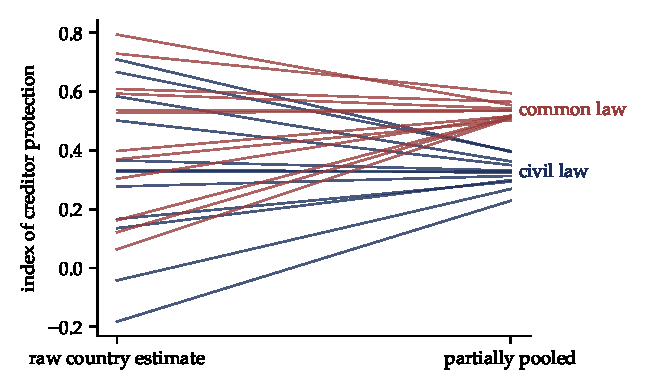
\includegraphics[width=\linewidth]{fig_shrinkage}
\caption{Partial pooling of country level estimates of creditor protection within two legal families, using simulated data. Raw estimates on the left are shrunk toward their family means, giving the partially pooled estimates on the right.}
\label{fig:shrinkage}
\end{figure}

\section{What we can conclude}

Taking the evidence as a whole, a reasonable posterior is roughly as follows. Legal rules protecting outside investors matter for financial development; this is supported by within country evidence from legal reforms as well as cross-country comparisons. Legal origin is correlated with those rules, but much less sharply than the original codings suggested, and it is confounded with other features of colonial history. The broader claim that legal origin represents a style of social control with wide consequences is plausible but less firmly established. And the mechanisms by which law affects finance, through courts, regulators, private enforcement and political economy, are only partly understood.

Two points from the debate are especially relevant to this book. First, enforcement matters as much as rules, and enforcement depends on courts. A rule protecting minority shareholders is worth little if courts take years to decide cases or decide them inconsistently. The procedural formalism documented in \emph{Courts} is a direct measure of how hard it is to obtain a decision. Second, the information that courts generate, in the form of reasoned decisions, is a public good that shapes behaviour. A system whose decisions are predictable reduces litigation and makes contracting cheaper. The Bayesian view of precedent in Chapter~\ref{ch:commoncivil} explains why: precedent is accumulated data about the law, and its value depends on its volume and consistency.

\section{From legal origin to legal technology}

The legal origins literature studied systems as they were in the late twentieth century. Technology is now changing how both traditions operate. Electronic filing, online dispute resolution and machine analysis of judgments reduce the cost of information about law and about cases. If formalism is costly because it slows proceedings and raises the cost of legal services, technology may reduce the penalty for formalism; if precedent is valuable because it accumulates information, machine learning may extract that information more effectively. The comparative advantage of each tradition may shift. Statute based rules are easier to formalise, as Catala shows; precedent based systems produce more data for learning. Chapter~\ref{ch:india} examines how a common law system under extreme load is responding with technology, and Chapter~\ref{ch:lean} how formal verification fits each tradition.

\section*{Notes and Questions}
\addcontentsline{toc}{section}{Notes and Questions}
\begin{enumerate}[label=\arabic*.]
\item List the six components of the antidirector rights index. For one country you know well, code each component and compare your coding with that in the original paper.
\item Suppose the observed index $I_c$ equals latent protection $P_c$ plus error with variance $\sigma^2$, and two independent codings differ by one point in mean squared difference. Estimate $\sigma^2$. By how much would the coefficient of $I_c$ in a regression of market size on $I_c$ be attenuated if the variance of $P_c$ were two?
\item Design a Bayesian model averaging exercise for the effect of legal origin on stock market capitalisation. Which candidate controls would you include? What prior over models?
\item Rajan and Zingales's great reversal shows that France's stock market was relatively large in 1913. Is this evidence against the legal origins thesis? What would a defender say?
\item The \emph{Courts} paper measured formalism for eviction and cheque collection. Propose a similar measure for the speed and consistency of decisions on commercial contracts, and explain how you would estimate it.
\item Explain why a hierarchical model with legal families as groups can reveal whether legal origin matters. What would you conclude if the posterior for between-family variance were concentrated near zero?
\end{enumerate}

\section*{Further reading}
The original papers \citep{llsv1997,llsv1998}; the 2008 survey \citep{lls2008}; \emph{Courts} \citep{djankov2003}; Spamann's recoding \citep{spamann2010}; Klerman and colleagues on colonial history \citep{klerman2011}; Roe on politics \citep{roe2003}.

\chapter{Africa as a Natural Experiment}
\label{ch:africa}

\section{A continent of transplanted law}

At the Berlin Conference of 1884 and 1885 and in the decades that followed, European powers divided Africa among themselves along lines that often cut across existing political, ethnic and economic boundaries. Each colonial power brought its own law. British colonies received the common law, statutes of general application and English procedure, administered alongside customary law through systems of indirect rule. French colonies received the Napoleonic codes and French administrative law, administered more directly. Belgian, Portuguese, German, Spanish and Italian colonies received their own versions of civil law. In southern Africa, Roman Dutch law, the law of the Cape Colony before British rule, persisted as a mixed system. Islamic law governed personal matters, and in places criminal matters, across the Sahel and the north. Customary law, in hundreds of local varieties, continued to govern land, marriage and succession for most of the population.\index{Africa!legal systems}

Independence, mostly in the 1950s and 1960s and later in Portuguese and southern Africa, left these systems largely in place. Ghana, Nigeria, Kenya, Uganda, Tanzania, Zambia and Sierra Leone remained common law countries; Senegal, C\^ote d'Ivoire, Mali, Burkina Faso, Niger, Gabon and others remained civil law countries; South Africa, Botswana, Zimbabwe, Namibia and Lesotho retained mixed systems. This history makes Africa, as many scholars have noted, a natural laboratory for the legal origins thesis of Chapter~\ref{ch:llsv}. Neighbouring countries with similar geography, peoples and pre colonial institutions received different legal systems for reasons that had little to do with local conditions. If legal origin matters for economic outcomes, Africa is where we should be able to see it most clearly.

The laboratory is imperfect. Colonial powers differed in much besides law: in their education policies, their use of indirect rule, their investment in infrastructure, their treatment of missionaries, their extraction of resources and their exit. Separating law from everything else that came with it is the central challenge, and it is a problem of Bayesian inference with confounding \citep{klerman2011}.

\section{Borders as experiments}

\subsection{The idea}

When a colonial border divides a homogeneous area, the populations on either side were similar before colonisation and differ afterwards mainly in what the colonisers did. Comparing outcomes close to the border, where geography and pre colonial institutions are nearly identical, isolates the effect of colonial rule. This is a regression discontinuity design: outcomes are modelled as smooth functions of distance from the border, with a jump at the border measuring the effect.\index{regression discontinuity}

Michalopoulos and Papaioannou used the partition of ethnic homelands by colonial borders to study the effects of national institutions on development across Africa. They found that within partitioned ethnic homelands, differences in national institutions on either side of a border had surprisingly little effect on local economic development except near the capitals, measured by night time light density \citep{michalopoulos2014}, while in companion work they found that pre colonial ethnic institutions are strongly associated with development today \citep{michalopoulos2013}. Their result is a caution for any theory that attributes African development mainly to national institutions inherited from colonisers.

\subsection{Cameroon}

Cameroon offers the sharpest experiment, because the border runs inside a single country. Germany colonised Kamerun in the 1880s. After the First World War Britain and France divided it, and the League of Nations confirmed the division as a larger French mandate and a smaller British mandate along the Nigerian border. At independence in 1960 and 1961 the French territory and the southern part of the British territory united to form a federal republic, later a unitary state. The Anglophone regions in the north west and south west retained the common law, English language courts and English procedure; the Francophone regions retained the civil law. The country is bijural.\index{Cameroon}

Lee and Schultz used the former boundary between the British and French mandates as a discontinuity, comparing rural areas on either side within a single country, so that national institutions after reunification are held fixed \citep{lee2012}. They reported that areas on the formerly British side had higher levels of some measures of household wealth and access to public goods such as piped water. Figure~\ref{fig:rd} illustrates the design with simulated data. The design separates colonial legacy from national policy, but it cannot separate law from the other legacies of British rule, such as language, education and local administration. A difference at the border is the effect of the colonial package.

\begin{figure}[t]
\centering
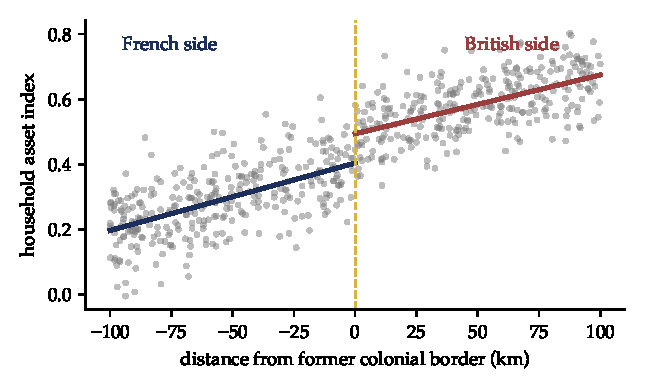
\includegraphics[width=\linewidth]{fig_rd}
\caption{A regression discontinuity across a former colonial border, with simulated data. The estimated jump at the border is the effect of the colonial package, of which the legal system is one component.}
\label{fig:rd}
\end{figure}

\subsection{A Bayesian border model}

A Bayesian analysis of border designs adds three things. First, it represents uncertainty about the functional form of the outcome as a function of distance, for instance with a flexible prior over smooth functions (a Gaussian process), so that the estimated jump does not depend on an arbitrary choice of polynomial. Second, it pools information across many borders with a hierarchical model, so that the effect at each border is estimated with the help of the others and the average effect of, say, British versus French rule is estimated with appropriate uncertainty. Third, it carries the uncertainty in each step through to the decomposition of the effect, using auxiliary data, into components attributable to different channels.

Let $y_{bi}$ be the outcome for location $i$ near border $b$, $x_{bi}$ its signed distance from the border, and $z_{bi}$ an indicator for the British side. A model is
\begin{equation}
y_{bi} = f_b(x_{bi}) + \delta_b z_{bi} + \epsilon_{bi}, \qquad \delta_b \sim N(\delta_0 + \gamma^\top w_b, \tau^2),
\label{eq:bordermodel}
\end{equation}
where $f_b$ is a smooth function, $\delta_b$ the jump at border $b$, $w_b$ border level covariates such as the difference in colonial education spending or in the share of indirect rule, and $\gamma$ their effects on the jump. If, after accounting for $w_b$, the residual jump $\delta_0$ is near zero, the evidence attributes the colonial effect to the measured channels rather than to law as such. If a legal variable, such as the presence of common law courts, has a large coefficient in $\gamma$, that is evidence for a legal channel.

\section{OHADA: harmonised business law}

In 1993, at Port Louis in Mauritius, a group of mainly Francophone African states signed a treaty establishing the Organisation for the Harmonisation of Business Law in Africa, known by its French acronym OHADA. Its members, now seventeen states mostly in West and Central Africa, adopt uniform acts that apply directly in each member state on subjects including general commercial law, company law, secured transactions, debt recovery, insolvency, arbitration and accounting. A Common Court of Justice and Arbitration in Abidjan serves as the supreme court for questions arising under the uniform acts, displacing national supreme courts in those matters.\index{OHADA}

OHADA is one of the largest experiments in legal harmonisation outside Europe. Its premise is that investors are deterred by fragmented, outdated and unpredictable business law, and that a single modern code applied by a common court would reduce uncertainty. In the terms of Chapter~\ref{ch:commoncivil}, OHADA strengthened the prior: it replaced many national rules with one set, and it created a court whose decisions accumulate across states, so that precedent, though formally not binding, is pooled. A hierarchical model of how courts apply the uniform acts would treat each state's courts as a group, with partial pooling toward the common court's interpretations.

Cameroon is an OHADA member, which raised a difficult question for its Anglophone regions: uniform acts drafted in the French civil law tradition had to be applied by common law courts. English translations of the acts were initially unavailable or unofficial, and common law lawyers objected to applying a civil law code in a common law jurisdiction. The tension was one strand of a wider grievance.

\section{The Anglophone crisis and the courts}

In late 2016 lawyers in Cameroon's Anglophone regions went on strike, protesting among other things the appointment of Francophone magistrates trained in the civil law to courts in the common law regions, the use of French in court proceedings there, and the failure to provide official English versions of OHADA acts. Teachers joined with parallel grievances about education. The protests were met with force, and the conflict escalated into an armed separatist insurgency and a humanitarian crisis that has continued for years.\index{Anglophone crisis}

The government's responses included the creation in 2017 of a common law division within the Supreme Court and, in 2018, a common law section at the national school for magistrates. These were attempts to preserve the bijural system by strengthening the institutions of the minority tradition. Whatever one thinks of the wider political conflict, its legal origins illustrate a point that cross country regressions cannot capture: legal systems are not only rules but communities of practitioners with shared training, language and expectations. A judge trained in one tradition, applying the procedural intuitions of that tradition in a court of the other, produces decisions that the parties perceive as illegitimate. In Bayesian terms, the judge's prior about how evidence should be presented and weighed does not match the parties', and the resulting decisions have high variance relative to what the parties can predict.

\section{Customary law and evidence}

For most Africans, customary law governs the most important matters in their lives: access to land, marriage, inheritance and the resolution of local disputes. British colonial regimes recognised customary law subject to a repugnancy clause, under which customs repugnant to natural justice, equity and good conscience would not be enforced. Post independence constitutions generally recognise customary law subject to fundamental rights.\index{customary law}

Customary law poses a distinctive evidence problem. Its content is not written in a code or in reported cases but held in the memory of elders and communities. In many jurisdictions courts must find it as a matter of fact, through the testimony of experts or assessors, unless it is notorious enough for judicial notice; a few, such as Ghana, treat it as a question of law. In Bayesian terms, the content of a customary rule is an unknown parameter about which the court receives noisy testimony, and the testimony may be shaped by the interests of the witnesses, since the rule on, say, women's inheritance rights affects who receives land. A coherent approach would treat each witness's account as a signal with an estimated reliability and a possible bias, and combine them as in Chapter~\ref{ch:graphs}, with the court mindful that the most authoritative witnesses may be those with the greatest stake.

\section{Election petitions: evidence at the highest stakes}

African courts have been asked to decide some of the highest stakes evidential questions any court faces: whether a presidential election was conducted so irregularly that it must be annulled. In September 2017 the Supreme Court of Kenya annulled the presidential election of the previous month, finding that the electoral commission had failed to conduct it in accordance with the constitution and the law, in particular in the transmission and verification of results. It was widely reported as the first time a supreme court in Africa had annulled a presidential election. In February 2020 the Constitutional Court of Malawi annulled the 2019 presidential election on the basis of widespread irregularities, and the Supreme Court of Appeal upheld the decision; the rerun election was won by the opposition candidate.\index{election petitions}

These cases raise in sharp form the questions of this book. What is the standard of proof for annulment? Most courts require the petitioner to show irregularities that affected the result, or that the conduct of the election so departed from the law that its result cannot be trusted. The first is a counterfactual question: would the result have been different without the irregularities? The second is a question about the integrity of a process. A Bayesian analysis of the first would model the vote counts at each polling station, the probability and size of irregularities, and the resulting uncertainty about the margin. If the margin is large relative to the plausible effect of irregularities, the posterior probability that they changed the result is small. If the margin is narrow, or the irregularities are widespread and unquantifiable, the posterior may be close to one half, and the decision must turn on the relative losses (the threshold of \eqref{eq:threshold}) of annulling a valid result and confirming an invalid one. Statistical methods for detecting anomalies in election returns, such as tests on the distribution of digits or of turnout and vote shares, are evidence of irregularity, but each has false positive rates that a court must understand.

The Kenyan and Malawian courts reasoned primarily about process: whether the law had been followed. A process based standard has the advantage that it does not require the court to estimate a counterfactual vote count, which may be impossible. It has the disadvantage that it can annul elections whose results were not in doubt. The decision theoretic framework does not choose between these standards, but it shows what each implies about the losses the court is weighing.

\section{Courts, contracts and development}

The \emph{Courts} study of Chapter~\ref{ch:llsv} \citep{djankov2003} found that procedural formalism is higher in civil law countries and associated with slower and less consistent decisions. Many African countries, both common law and civil law, have slow courts and large backlogs. For a small business, the expected value of a contract claim is the probability of winning times the amount, minus costs, discounted for delay. If a commercial case takes several years to resolve, the discounted value of a claim may be small, and the threat of litigation provides weak incentives to perform. Businesses respond by contracting only with those they know, relying on reputation and relationships rather than courts, which is the subject of Chapter~\ref{ch:gould}.

Technology offers some hope. Several African judiciaries have introduced electronic case management, filing and virtual hearings, especially since the pandemic. Specialised commercial courts, small claims procedures and arbitration centres aim to provide faster resolution for commercial disputes. The question for evaluation is whether these reforms change the posterior that a businessperson holds about the likely outcome and timing of a dispute, and thereby change behaviour. Randomised and quasi experimental evaluations, analysed with hierarchical Bayesian models that pool across courts and countries, are the natural tool.

\section{Lessons}

Africa shows that legal origin is one of many colonial legacies, and that its effects cannot be read off cross country regressions. Border designs isolate colonial effects but not the legal component of them. Bijural states such as Cameroon show that legal systems are communities of practice, and that the coexistence of traditions requires institutions that respect both. OHADA shows the attractions and the difficulties of harmonisation. Customary law and election petitions pose evidential problems of their own. Throughout, a Bayesian approach clarifies what the evidence can and cannot establish and what decisions under uncertainty require.

\section*{Notes and Questions}
\addcontentsline{toc}{section}{Notes and Questions}
\begin{enumerate}[label=\arabic*.]
\item In the border model \eqref{eq:bordermodel}, suppose there are ten borders with estimated jumps and standard errors of your choice. Compute the partially pooled estimates and the posterior for $\delta_0$ under a normal prior, treating $\tau$ as fixed and then as given a prior of your choice.
\item Lee and Schultz compare areas within Cameroon. What advantages does this have over comparing Nigeria and Cameroon at their international border? What does it not control for?
\item Design an evidentiary procedure for finding the content of a customary rule of inheritance, given that the most knowledgeable witnesses may have an interest in the outcome.
\item In a presidential election with ten million votes cast and a winning margin of two hundred thousand, irregularities are found at five per cent of polling stations. Under what assumptions about the size and direction of the irregularities would the posterior probability that they changed the result exceed one half?
\item OHADA's uniform acts apply directly in member states and are interpreted by a common court. In what sense does this pool precedent? What are the risks for a common law region within a member state?
\item Is a process based standard for annulling elections better than an outcome based standard? Answer in terms of the losses from each kind of error.
\end{enumerate}

\section*{Further reading}
Michalopoulos and Papaioannou on national institutions and partitioned ethnic groups \citep{michalopoulos2014}; Lee and Schultz on Cameroon \citep{lee2012}; Klerman and colleagues on colonial history \citep{klerman2011}.

\chapter{The Indian Court System}
\label{ch:india}

\begin{quote}\itshape
Law is the method, the manner in which our mind grasps a series of phenomena; it is all in the mind.
\par\hfill\normalfont Swami Vivekananda, \emph{Karma Yoga}
\end{quote}

\section{A common law system at scale}

India inherited the common law from British rule and has developed it into one of the world's most important legal systems. Its Supreme Court is among the most powerful constitutional courts anywhere; its High Courts have broad original and writ jurisdiction; its district and subordinate courts handle tens of millions of matters. It also carries the largest judicial backlog in the world. In July 2026 the Law Minister told Parliament, citing the National Judicial Data Grid, that more than $4.99$ crore cases were pending in subordinate courts, about $64.67$ lakh in the High Courts and about ninety three thousand in the Supreme Court (the last figure as on 28 July 2026), some $5.6$ crore, or fifty six million, in all. Parliamentary replies the same month put the High Court cases pending for more than thirty years at over seventy thousand (71,204 as on 24 July, 80,634 as on 28 July).\index{India!pendency}

This chapter describes the structure of the Indian courts, the evidence law that governs them, the causes and consequences of delay, and the use of data and technology to manage it. Its main argument is that delay is a decision problem: a court system with fixed capacity must decide which cases to hear, in what order, and how much time to give each, and Bayesian decision theory gives a principled way to make those choices.

\section{Vivekananda on law}

Swami Vivekananda, lecturing in America and England in the 1890s, gave an account of law that a Bayesian will find congenial. In his lectures on Karma Yoga he defined law as the tendency of a series to repeat itself, and argued that our idea of law arises from association: when phenomena recur in a regular order, the mind forms the expectation that they will recur, and that expectation is what we call a law. He connected this with the notion that the Nyaya school of Indian logic called \emph{vyapti}, the invariable concomitance on which inference rests \citep{vivekananda1896}. Law, he concluded, is the method, the manner in which our mind grasps a series of phenomena.\index{Vivekananda, Swami}\index{vyapti}

Vivekananda was speaking of natural and spiritual law, not of statutes. But his account describes the common law closely. A rule of the common law is the regularity a court perceives in a series of decided cases; precedent is the expectation that like cases will be decided alike; and a judge who distinguishes a precedent is recognising that the series does not extend to the case before her. In the hierarchical model of Chapter~\ref{ch:commoncivil}, the rule is the posterior summary of many decisions, the unity found in their variety. The Nyaya theory of inference, which required that the concomitance on which an inference rests be established by repeated observation and checked against counterexamples, is a theory of induction from cases of the kind the common law practises. India's courts, which apply a common law inherited from England in a country whose own traditions of logic and law are far older, are a natural place to notice the connection.

\section{Structure}

\subsection{The courts}

The Supreme Court, established by Article 124 of the Constitution, hears appeals from the High Courts and petitions for the enforcement of fundamental rights under Article 32. Under Article 136 it may grant special leave to appeal from any judgment of any court or tribunal, a discretionary jurisdiction that brings a large number of petitions to the Court. Under Article 142 it may pass any decree or order necessary for doing complete justice in any cause before it. The High Courts, twenty five in number, have supervisory jurisdiction under Article 227 and writ jurisdiction under Article 226 that is wider than the Supreme Court's, since it extends to the enforcement of legal rights generally. Below them, district courts and subordinate courts, civil and criminal, handle the great majority of cases.\index{Supreme Court of India}

\subsection{Public interest litigation}

From the late 1970s the Supreme Court relaxed rules of standing and procedure to allow public interest litigation. Letters to judges were treated as petitions; the Court appointed commissions to gather facts; and it issued continuing orders supervising government action. In \emph{Hussainara Khatoon v Home Secretary, State of Bihar}, a 1979 case brought on the basis of newspaper reports, the Court held that the right to a speedy trial is part of the right to life and personal liberty under Article 21 and ordered the release of undertrial prisoners who had been detained for longer than the maximum sentence for the offences charged \citep{hussainara1979}. Public interest litigation gave the Court a role in governance unmatched by most courts, and it also added to the Court's load.\index{public interest litigation}

\subsection{Lok Adalats}

The Legal Services Authorities Act 1987 gave statutory status to Lok Adalats, people's courts, which resolve disputes by conciliation and compromise. An award of a Lok Adalat is deemed a decree of a civil court and is final, with no appeal. National Lok Adalats held on single days across the country dispose of large numbers of matters, both pending cases and disputes at the pre litigation stage, especially in motor accident claims, cheque dishonour, family disputes and bank recovery. They are a parallel disposal channel that relies on the parties' willingness to settle.\index{Lok Adalat}

\section{The law of evidence}

\subsection{Stephen's definition of proof}

The Indian Evidence Act 1872 was drafted by James Fitzjames Stephen, who sought to codify the English law of evidence in a form that Indian judges, many of them not trained in English law, could apply. Section 3 defined proof in terms that a decision theorist would recognise:
\begin{quote}
A fact is said to be proved when, after considering the matters before it, the Court either believes it to exist, or considers its existence so probable that a prudent man ought, under the circumstances of the particular case, to act upon the supposition that it exists.
\end{quote}
The definition has two parts. The first is belief. The second is probability combined with action: the fact is proved when its probability is high enough that a prudent person ought to act on it under the circumstances. That is the decision theoretic standard of Chapter~\ref{ch:standards}: a posterior threshold that depends on the consequences of acting, which differ from case to case. Stephen wrote, nearly a century before Kaplan, a definition of proof that ties the threshold to the stakes.\index{Indian Evidence Act}\index{Stephen, James Fitzjames}

The Indian courts have read the definition as permitting different standards in criminal and civil cases, with proof beyond reasonable doubt required in the former, and as emphasising the prudent man's judgment in the circumstances. In 2023 Parliament replaced the Indian Penal Code, the Code of Criminal Procedure and the Evidence Act with three new statutes, the Bharatiya Nyaya Sanhita, the Bharatiya Nagarik Suraksha Sanhita and the Bharatiya Sakshya Adhiniyam, which came into force in July 2024. The new evidence statute retains Stephen's definitions of proved, disproved and not proved, while modernising provisions on electronic records.

\subsection{Presumptions}

Stephen's Act also codified presumptions, including the court's power under section 114 to presume the existence of any fact it thinks likely to have happened, having regard to the common course of natural events, human conduct and public and private business. The illustrations to the section are a catalogue of prior probabilities: that a man in possession of stolen goods soon after the theft is either the thief or has received the goods knowing them to be stolen, unless he can account for his possession; that an accomplice is unworthy of credit unless corroborated in material particulars; that a bill of exchange was accepted for good consideration. Each presumption is a default probability given the basic fact, which serves as the prior for any rebutting evidence. The Bayesian framework explains why presumptions are useful: they economise on proof by fixing the prior where experience supports it, and they place the burden of producing contrary evidence on the party best placed to produce it.

\section{Delay}

\subsection{Causes}

Many causes of delay have been identified: too few judges relative to population and caseload, vacancies in sanctioned posts, frequent adjournments, the government's role as the largest litigant and its tendency to appeal adverse decisions, procedural complexity, the volume of minor cases such as cheque dishonour prosecutions, and inadequate infrastructure. The Law Commission recommended in its 1987 report a ratio of fifty judges per million population; the actual ratio has remained a fraction of that.\index{judge population ratio}

\subsection{Consequences}

Delay imposes direct costs on litigants and indirect costs on the economy. For criminal defendants held in custody awaiting trial, delay is punishment without conviction. Undertrial prisoners make up a large majority of India's prison population, and many are poor and unable to meet bail conditions. For commercial parties, delay reduces the value of contracts, as Chapter~\ref{ch:africa} described for African courts, and encourages reliance on relationships rather than law. For the legitimacy of the courts, delay undermines the belief that rights can be enforced.

\section{A queueing model}

A court system is a queue. Cases arrive, wait, are served and leave. Let $B_t$ be the number of pending cases at the start of year $t$, $A_t$ the number filed during the year and $D_t$ the number disposed of. Then
\begin{equation}
B_{t+1} = B_t + A_t - D_t .
\end{equation}
If arrivals exceed disposals, the backlog grows without bound. If disposals exceed arrivals, it shrinks. Little's law, a basic result of queueing theory, says that in a steady state (arrivals equal to disposals, which only roughly describes India) the average time a case spends in the system equals the average number pending divided by the throughput:
\begin{equation}
\bar W = \frac{\bar B}{\bar D}.
\end{equation}
With a backlog of about $5.6$ crore and annual disposals of the order of two to two and a half crore, the average time in the system is two to three years, and the distribution is highly skewed, with some cases pending for decades.\index{queueing model}\index{Little's law}

Figure~\ref{fig:indiabacklog} shows stylised backlog paths under different disposal rates, holding arrivals fixed. The point is the sensitivity: a small excess of arrivals over disposals produces steady growth, and even a disposal rate a sixth above arrivals takes fourteen years to clear the backlog. Raising disposals requires more judges, fewer adjournments, simpler procedures or diversion of cases to other channels such as Lok Adalats.

\begin{figure}[t]
\centering
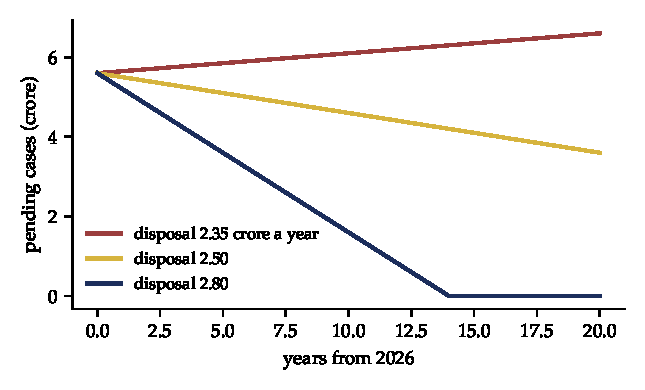
\includegraphics[width=\linewidth]{fig_india_backlog}
\caption{Stylised paths of the total pending caseload under three annual disposal rates, starting from $5.6$ crore with arrivals fixed at $2.4$ crore a year. Illustrative values, not forecasts.}
\label{fig:indiabacklog}
\end{figure}

\section{Bayesian triage}

\subsection{Which cases first}

If a court cannot hear every case promptly, it must decide which to hear first. The default in most courts is first come, first served, modified by statutory priorities and judicial discretion. Queueing theory offers a better rule when cases differ in the cost of delay and in the time needed to decide them. The $c\mu$ rule says that to minimise the total cost of waiting, when delay costs are linear in time and there is a single server, a server should give priority to the class of jobs with the highest product of the cost of delay per unit time, $c$, and the service rate, $\mu$, the reciprocal of the expected service time. Short cases with high costs of delay go first; long cases with low costs of delay wait.\index{c mu rule}

In a court, the cost of delay depends on the case: an undertrial prisoner's detention, a family without access to its land, a business with funds frozen. The service time depends on the complexity of the case and the likelihood of adjournment. Neither is known exactly at filing. A Bayesian triage system would estimate both from the case's features, using a hierarchical model trained on past cases, and would update the estimates as the case progresses. The priority index for case $j$ is then
\begin{equation}
\pi_j = \frac{\E[c_j \given \text{data}]}{\E[1/\mu_j \given \text{data}]},
\end{equation}
the expected cost of delay divided by the expected service time, or, taking account of uncertainty, a quantity such as the Gittins index, which values a case by the best long-run rate of return from working on it and so rewards learning about uncertain cases.

\subsection{Value of information}

Some cases can be resolved quickly once a single question is answered: whether a cheque was presented within time, whether a notice was served, whether the parties are willing to compromise. The value of information calculation of Chapter~\ref{ch:standards} identifies cases where a small investment of judicial time would likely produce a disposal. A triage system that screens cases for such questions, perhaps referring them to a short hearing or to a Lok Adalat, could raise disposals without new judges.

\subsection{Adjournments}

Adjournments are a major cause of delay. Each adjournment is a decision by the court to postpone, often at a party's request. A model of adjournments would estimate the probability that a hearing results in adjournment as a function of the case, the stage, the parties and the court, and would identify where adjournments are concentrated. Reforms such as costs on parties who seek adjournments, limits on their number, or case management conferences that fix timetables, can then be targeted. The data to estimate such models exist in the National Judicial Data Grid.

\section{Data and technology}

\subsection{The National Judicial Data Grid}

The eCourts project, a mission mode programme of the government and the judiciary, has computerised the district courts and created the National Judicial Data Grid, a public platform that reports pending and disposed cases by court, case type and age, updated continuously. The Grid makes Indian court data among the most accessible in the world. It allows researchers, journalists and the courts themselves to see where backlogs are concentrated and how they change. It is the foundation for any data driven approach to court management.\index{National Judicial Data Grid}

\subsection{Artificial intelligence}

The Supreme Court has introduced artificial intelligence tools for translation of judgments into Indian languages and for assisting judges with research. The use of such tools raises the questions to which Chapter~\ref{ch:lindleyai} returns: accuracy, bias, transparency and the proper division of labour between the machine and the judge. For a court system under the load India's carries, the potential benefits of automation in routine tasks, such as scheduling, translation, document review and the identification of similar cases, are large. The risks are greatest where machines would make or shape decisions on liberty or rights, and there the Bayesian requirements of calibration and explicit uncertainty are most important.

\section{Bail as expected utility}

The bail decision illustrates the use of probability in an Indian court under load. A magistrate deciding whether to release an accused before trial must weigh the risk that the accused will abscond, tamper with evidence or commit further offences against the cost of detention to the accused, who is presumed innocent and may wait years for trial. Let $r$ be the probability of a harmful event if released, $H$ the harm, and $C$ the cost of detention (the loss called $D$ in Chapter~\ref{ch:decisions}, renamed here because $D_t$ denotes disposals) over the expected time to trial $T$. Release is the better decision if
\begin{equation}
r\,H < (1-r)\,C(T),
\end{equation}
as in Chapter~\ref{ch:decisions}, and $C(T)$ grows with $T$. In a system where trials take years, $C(T)$ is large, and release should be the norm for all but high risk accused. In \emph{State of Rajasthan v Balchand} (1977) the Supreme Court put the basic rule as \textquotedblleft bail, not jail\textquotedblright, and it has repeated since that bail is the rule and jail the exception. The decision theoretic analysis supports that principle, and shows that it becomes stronger as delay increases. Risk assessment tools that estimate $r$ could help magistrates, but they must be calibrated on Indian data and checked for bias, as Chapter~\ref{ch:lindleyai} explains.

\section{Lessons}

India shows that the common law's reliance on courts to resolve disputes and make law requires courts with capacity to match demand. When capacity falls short, delay becomes the dominant feature of the system, and the theoretical virtues of adversarial procedure and precedent are swamped. Stephen's Evidence Act, with its decision theoretic definition of proof, shows that decision theoretic ideas were built into Indian evidence law from 1872. The National Judicial Data Grid shows what transparency about the state of the courts can achieve. The next step is to use those data for decisions: which cases to hear, which to divert, how to schedule, and when to release. Each is a decision under uncertainty, and each can be improved by explicit probabilities and costs.

\section*{Notes and Questions}
\addcontentsline{toc}{section}{Notes and Questions}
\begin{enumerate}[label=\arabic*.]
\item Read section 3 of the Indian Evidence Act and section 2 of the Bharatiya Sakshya Adhiniyam. Express the definition of proved as a decision rule. What role does the phrase under the circumstances of the particular case play?
\item Using Little's law, compute the average time to disposal for a court with a backlog of two hundred thousand cases and annual disposals of eighty thousand. What disposal rate would halve it?
\item A court has two classes of case: bail applications with an expected hearing time of ten minutes and a cost of delay of one unit per day, and civil suits with an expected hearing time of three hours and a cost of delay of two units per day. Apply the $c\mu$ rule.
\item Section 114 of the Evidence Act allows courts to presume facts likely to have happened. Choose three illustrations to the section and state the prior probability each implicitly assumes.
\item Design a Bayesian model of adjournments using data of the kind available in the National Judicial Data Grid. What variables would you include, and how would you use the model to target reform?
\item Using the bail inequality, find the maximum risk of absconding at which release is optimal if the harm from absconding is ten units, the cost of detention is one unit per month and the expected time to trial is two years.
\end{enumerate}

\section*{Further reading}
The National Judicial Data Grid is the primary source for data. Stephen's own \emph{Digest of the Law of Evidence} explains his approach. On public interest litigation, \emph{Hussainara Khatoon} \citep{hussainara1979}.

\chapter{Arbitration, Mediation and Private Adjudication}
\label{ch:arbitration}

\section{Choosing a forum}

Courts are not the only adjudicators. Commercial parties routinely agree to resolve disputes by arbitration, choosing their arbitrators, procedure, seat and governing law. Investors and states arbitrate under bilateral investment treaties. Consumers and employees, particularly in the United States, are often bound by arbitration clauses in standard contracts. Mediation, in which a neutral helps the parties reach their own agreement, has become a routine step in civil litigation in many systems. Each of these forums makes decisions under uncertainty, and the choice among them is itself a decision. This chapter applies the framework of the book to private adjudication and to the choice of forum.\index{arbitration}\index{mediation}

\section{Why parties arbitrate}

Parties choose arbitration for several reasons: neutrality, especially in international disputes where neither party trusts the other's courts; expertise, since arbitrators can be chosen for knowledge of the industry; confidentiality; speed and finality, since grounds for setting aside an award are narrow; and enforceability, since the New York Convention\index{New York Convention} of 1958 makes arbitral awards enforceable in more than one hundred and fifty countries. Each reason can be expressed in the terms of this book. Neutrality and expertise affect the accuracy of the decision, the location of the ROC curve in Chapter~\ref{ch:decisions}. Speed reduces the cost of delay. Finality trades the error correcting value of appeals, taken up in Chapter~\ref{ch:systemcosts}, for lower cost and certainty. Enforceability raises the probability that a favourable decision produces a recovery.

\section{Arbitrator selection as a game}

In a three member tribunal, each party appoints one arbitrator and the two, or an institution, choose the chair. In international arbitration, party appointed arbitrators are required to be independent and impartial, but each party will appoint someone it expects to be receptive to its arguments. The setting resembles the adversarial expert problem of Chapter~\ref{ch:fienberg}: each side selects from a distribution of possible arbitrators, and the outcome depends heavily on the chair. Research on investment arbitration has examined whether arbitrators' prior decisions predict their votes, and whether repeat appointments create incentives to favour the parties who appoint. A Bayesian analysis treats each arbitrator's tendencies as a parameter estimated from past decisions, with shrinkage toward the mean for arbitrators with few decisions, and asks how much the composition of a tribunal changes the predicted outcome.

\section{Consumer and employment arbitration}

In the United States, the Supreme Court has enforced arbitration clauses in consumer and employment contracts, including clauses that waive class actions, under the Federal Arbitration Act, in decisions such as \emph{AT\&T Mobility v Concepcion} and \emph{Epic Systems v Lewis} \citep{concepcion2011,epic2018}. Critics argue that such clauses suppress small claims, which are uneconomic to arbitrate individually, and so reduce the deterrent effect of consumer and employment law. The analysis developed in Chapter~\ref{ch:funding} explains why: aggregation is what makes small claims viable, and a class waiver removes it. In decision theory terms, if individual claims have expected value below their cost, none is brought, and the expected liability of a firm that causes many small harms falls toward zero, weakening its incentive to avoid them, as in the Becker framework developed in Chapter~\ref{ch:becker}.

\section{Mediation and the zone of agreement}

Mediation succeeds when the parties' settlement ranges overlap and fails when they do not. The settlement model developed in Chapter~\ref{ch:becker} shows that the range exists when the parties' disagreement about the outcome, multiplied by the stakes, is less than their combined costs of continuing. A mediator can create or widen the zone in three ways: by narrowing the parties' disagreement about the probability of success, often by testing each side's view of the evidence in private sessions; by adding terms that create value for both, which enlarges the joint gain from agreement; and by making the costs of continuing salient. The first is Bayesian updating guided by a neutral: a mediator who shows each party the weaknesses in its case moves its posterior toward the other's.

The English courts have encouraged mediation through costs sanctions for unreasonable refusal, and in \emph{Churchill v Merthyr Tydfil County Borough Council} the Court of Appeal held in 2023 that courts may lawfully order parties to engage in non court based dispute resolution \citep{churchill2023}. The decision theoretic justification is that mediation is cheap relative to trial and has a real chance of producing settlement, so its expected value is positive in many cases even if it often fails.

\section{Investment arbitration and states}

Investment treaty arbitration allows foreign investors to bring claims against states for expropriation and unfair treatment before international tribunals. Awards can be very large, and states have criticised the system for inconsistency and for the influence of arbitrators who also act as counsel. Reforms under discussion include an appellate mechanism and a permanent investment court. The analysis of appeals developed in Chapter~\ref{ch:systemcosts} applies: an appellate body would reduce inconsistency, a form of noise, and correct errors, at the cost of finality and delay. Whether the trade off is worthwhile depends on the size of the errors and inconsistency in the current system, which can be estimated from the record of awards.

\section{Online dispute resolution}

For small disputes, online dispute resolution\index{online dispute resolution} offers faster and cheaper resolution than courts. Marketplaces resolve millions of disputes between buyers and sellers each year through online processes, mostly automated. Public bodies have adopted similar approaches, such as British Columbia's Civil Resolution Tribunal taken up in Chapter~\ref{ch:lindleyai}. These systems are where machine assisted adjudication is most advanced, because the stakes per case are small and volumes large. They show what is possible and what must be guarded against: decisions that are fast but opaque, consistent but not contestable. The requirements that Chapter~\ref{ch:lindleyai} sets out for machine adjudication, transparency and contestability among them, apply here first.

\section*{Notes and Questions}
\addcontentsline{toc}{section}{Notes and Questions}
\begin{enumerate}[label=\arabic*.]
\item A commercial party estimates that a court would decide its dispute correctly with probability $0.85$ after three years and costs of two million, and an arbitral tribunal with probability $0.80$ after eighteen months and costs of one and a half million, with no appeal. Which forum should it prefer for a claim of twenty million with a true probability of success of $0.7$?
\item Explain why class action waivers in consumer arbitration clauses can reduce deterrence. Use the expected value of an individual claim.
\item In a mediation, the claimant believes it will win with probability $0.7$ and the defendant believes $0.4$, with stakes of one million and costs of one hundred thousand each. Is there a zone of agreement? What must the mediator change to create one?
\item Should investment arbitration have an appellate body? Frame your answer as a value of information calculation.
\end{enumerate}

\section*{Further reading}
\emph{AT\&T Mobility v Concepcion} \citep{concepcion2011}; \emph{Churchill v Merthyr Tydfil} \citep{churchill2023}.


\part{Order Without the State}
\chapter{Vendetta, Honour and the Mafia}
\label{ch:gould}

\section{Order without courts}

Courts are one solution to the problem of social order. When a person is wronged, the state hears the claim, finds the facts and enforces a remedy. Where courts are absent, distant, slow or untrusted, people find other solutions. Families avenge their members. Communities ostracise wrongdoers. Merchants trade only with those whose reputations they know. Private organisations sell protection. These alternatives are not merely primitive versions of law. They are institutions with their own logic, and that logic is in large part a logic of signals and inference: of revealing and learning who can be trusted, who will retaliate and who is strong.\index{social order}

This chapter examines two bodies of work on order without effective state courts. Roger Gould, a sociologist who taught at the University of Chicago and Yale before his early death in 2002, studied vendetta in nineteenth century Corsica and developed a general theory of interpersonal conflict \citep{gould2000,gould2003}. Diego Gambetta studied the Sicilian mafia as an industry selling private protection \citep{gambetta1993}. Gould's empirical work was on Corsica, the French Mediterranean island whose clan structure, honour culture and weak state presence closely resembled those of Sicily, and Gambetta's on Sicily itself. Together they show how Bayesian ideas about signals, reputations and uncertain rank illuminate societies where the courts do not settle disputes.

\section{Gould on Corsican vendetta}

\subsection{The puzzle}

Corsica was famous in the nineteenth century for vendetta. Novels such as Prosper M\'erim\'ee's \emph{Colomba} portrayed a society in which families were bound by an iron duty to avenge their dead, and in which feuds persisted for generations. Social scientists attributed vendetta to a culture of collective honour and collective responsibility: an injury to one was an injury to the whole kin group, and any member of the offender's group was a legitimate target.\index{Corsica}\index{vendetta}

Gould tested this account against evidence. He used French court records of violent incidents in Corsica in the second half of the nineteenth century, which recorded the relationships between offenders, victims and others involved \citep{gould2000}. From these he could estimate how often killings were avenged, what predicted revenge, and who was targeted.

\subsection{Findings}

Gould's findings contradicted the cultural account in several respects. Vengeance was rare: most killings were not avenged at all. When vengeance occurred, it typically followed incidents in which the original attack had involved collaboration among several members of the offender's group, or violence against people who were not parties to the dispute. Vengeance rarely extended beyond the nuclear family; when it did, correspondingly distant kin of the victim acted as avengers. And the targets of revenge were selected on the basis of specific acts of solidarity with the original offender, such as participating in the attack or sheltering the killer, not on abstract collective responsibility.

Gould concluded that vengeance was a purposeful sanction against collective aggression, calibrated to demonstrate that the aggrieved family's cohesiveness matched that displayed by the offender's group. Vendettas were strategic yet altruistic acts: strategic because they responded to specific displays and were scaled to them, altruistic because the avenger bore risk on behalf of the group.

\subsection{A Bayesian reading}

Gould's account is naturally expressed in terms of signals. When a group acts together in violence, it reveals its cohesion: its members are willing to bear risk for each other. Other groups update their beliefs about the group's strength. A family that is attacked by a cohesive group and does not respond reveals, or is taken to reveal, that it lacks the cohesion to defend itself, and its posterior strength in the eyes of others falls. Further aggression against it becomes more attractive. Revenge restores the family's reputation by matching the signal: it demonstrates cohesion of the same degree.\index{costly signalling}

When the original attack was by a single individual acting alone, it revealed nothing about the cohesion of his group, and failure to respond carried no reputational cost to the victim's family as a group. Revenge was then unnecessary from the point of view of reputation, and the costs of violence, including prosecution by the French state, dominated. This would explain why revenge was rare after individual attacks and more common after collective ones. Figure~\ref{fig:vendetta} illustrates the pattern with a stylised model in which the probability of revenge rises with the size of the victim's kin group and with the degree of collaboration in the original attack.

\begin{figure}[t]
\centering
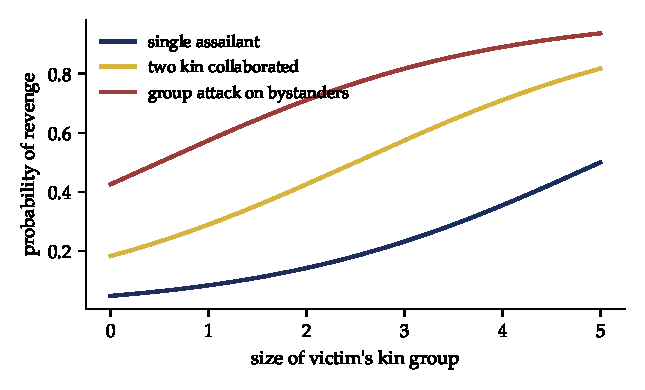
\includegraphics[width=\linewidth]{fig_vendetta}
\caption{A stylised model of the probability of revenge as a function of the size of the victim's kin group, for three kinds of original attack: a single assailant, two kin collaborating, and a group attack on bystanders. Collective attacks and attacks on bystanders, which signal the offender group's cohesion, make revenge more likely. Illustrative, not estimated from Gould's data.}
\label{fig:vendetta}
\end{figure}

The selection of targets follows the same logic. An avenger who killed an arbitrary member of the offender's kin would signal only a willingness to kill. One who killed a person who had displayed solidarity with the offender, by joining the attack or hiding him, signalled that the family would respond precisely to acts of solidarity, raising the cost of such acts in the future. Revenge was a sanction, and sanctions deter only if they are targeted at the conduct to be deterred.

\subsection{Vendetta and the state}

Gould's Corsica was not stateless. It was a French department with courts, prosecutors and gendarmes, and the records he used were produced by them. But the state's reach was limited, its legitimacy contested, and its procedures slow. Families could not rely on the courts to protect them or to deter aggressors. Vendetta coexisted with prosecution: an avenger might be prosecuted, and the prosecution might itself be part of the feud, as families used the courts against each other. Stephen Wilson's history of feuding and banditry in nineteenth century Corsica documents the complex interplay between local sanctions and the French judicial system \citep{wilson1988}. The Bayesian point is that families acted on their beliefs about the probability and speed of state enforcement. Where those beliefs were pessimistic, private enforcement filled the gap.

\section{Gould on ambiguous rank}

\subsection{Collision of Wills}

In \emph{Collision of Wills}, published posthumously in 2003, Gould developed a general theory of interpersonal conflict \citep{gould2003}. His central claim was that conflict is most likely in relationships where social rank is ambiguous. In clearly hierarchical relationships, such as parent and young child or employer and employee, each party knows its place, and disputes are resolved by deference. Relationships between equals or near equals are the hardest case, because symmetry leaves relative rank open: neither party has a ready claim to the other's deference. Violence arises when the relative standing of the parties is uncertain or contested: when each believes it is entitled to the other's deference, or when a challenge to one's standing cannot be ignored without accepting a lower position. Gould drew on evidence from homicide records in Corsica and elsewhere, showing that many killings arose from trivial disputes between people of similar status, in which the stakes were not the trivial object but the relationship.\index{Collision of Wills}\index{ambiguous rank}

\subsection{Rank as a posterior}

Gould's theory has a direct Bayesian interpretation. Each party holds a belief about the relative standing of the two: the probability that, if the matter came to a contest, the other would yield. Call party $A$'s belief $p_A$ that $B$ would yield, and $B$'s belief $p_B$ that $A$ would yield. If one belief is near one and the other near zero, so that both agree who would yield, there is no conflict: the subordinate yields. If the beliefs are inconsistent, each expecting the other to yield, both stand firm, and conflict follows. Inconsistent beliefs are most likely when the evidence about relative standing is weak or ambiguous, that is, when the posterior is near one half and each party's prior or interpretation, assumed to be self-serving, pushes it in its own favour.

The same structure appears in theories of litigation and war. Priest and Klein, whose model Chapter~\ref{ch:becker} develops, showed that cases go to trial when the parties' estimates of the outcome diverge, and that this happens most often when the case is close \citep{priest_klein1984}. James Fearon argued that wars occur when states have private information about their strength and incentives to misrepresent it, so that their estimates of the outcome of a war diverge \citep{fearon1995}. Gould's theory applies the same logic to individuals. Conflict is the product of disagreement about a posterior, and disagreement is most likely when the evidence is ambiguous.

The implication for law is that clarifying rights reduces conflict. Where property boundaries are uncertain, disputes are frequent; where they are surveyed and registered, disputes are rare. Where the hierarchy of a workplace is clear, there are fewer personal conflicts than where roles overlap. Legal rules that make entitlements clear move the posterior away from one half and reduce the scope for collisions of will. This is a Bayesian argument for clear rules, complementary to the economic argument from transaction costs.

\section{Gambetta on the Sicilian mafia}

\subsection{An industry of protection}

Diego Gambetta's \emph{The Sicilian Mafia: The Business of Private Protection} argued that the mafia is best understood not as a criminal organisation that engages in many illegal activities, but as a set of firms that sell a single product, protection \citep{gambetta1993}. In a market economy, people need assurance that their trading partners will honour agreements, that their property will not be stolen, and that competitors will not use violence against them. Where the state provides these assurances reliably, through courts and police, the demand for private protection is small. Where it does not, people will pay for protection from whoever can supply it credibly. In western Sicily after Italian unification, the state was weak and distrusted, property rights were in flux following the abolition of feudalism, and a market for private protection developed.\index{Gambetta, Diego}\index{mafia}

The product is trust. A mafioso guarantees transactions: he ensures that a buyer of cattle receives the animals promised, that a cartel of contractors keeps to its agreement, that a merchant is not robbed. His guarantee is credible because he can and will use violence against those who break the agreement. His customers pay for this guarantee, and sometimes they are coerced into paying, since the protector who can punish cheats can also punish those who decline his services.

\subsection{Reputation as a posterior}

The mafioso's capital is his reputation for violence. Reputation is a posterior: others' belief about whether he will carry out his threats. A credible reputation allows him to protect without using violence, since threats suffice. Violence is costly and attracts the attention of the state, so a protector with a strong reputation uses it rarely. But reputation decays if never tested, and imitators can claim a reputation they have not earned. The mafia's elaborate signals, its rituals of initiation, its codes of conduct and its restrictions on membership, can be read as ways of making the signal of membership hard to fake, so that the reputation of the organisation attaches credibly to its members. Gambetta's later book \emph{Codes of the Underworld} analysed how criminals signal to each other in a world where they cannot rely on courts to enforce agreements or on ordinary signals to be honest \citep{gambetta2009}.\index{reputation}

\subsection{Origins: land, sulphur and lemons}

Economists have tested theories of the mafia's origins using variation across Sicilian towns in the nineteenth century. Bandiera argued that the breakup of feudal estates and the resulting fragmentation of land ownership increased the demand for protection, and showed that mafia presence was associated with land fragmentation \citep{bandiera2003}. Buonanno, Durante, Prarolo and Vanin found that mafia presence in the 1880s was associated with the location of sulphur mines, a valuable resource in a weak state environment \citep{buonanno2015}. Dimico, Isopi and Olsson argued that the mafia arose where the export of citrus fruit, highly profitable and vulnerable to theft, created a strong demand for protection \citep{dimico2017}. Each theory identifies a source of demand for protection where the state's supply was deficient. A Bayesian comparison of these theories would ask which predicts the pattern of mafia presence across towns best, accounting for the correlation between the proposed causes and for spatial correlation among neighbouring towns.

\section{The state strikes back: the maxi trial}

\subsection{Evidence from the inside}

The mafia's power rested in part on \emph{omert\`a}, the code of silence that made witnesses unwilling to testify. Without witnesses, prosecutions failed. In 1982 Italy introduced the crime of mafia type association, Article 416 bis of the penal code, which made membership in an organisation using intimidation and subjection to commit crimes or acquire control of economic activities an offence, and allowed confiscation of assets. In 1984 Tommaso Buscetta, a senior mafioso whose brother, son-in-law, nephews and other relatives had been killed in a war between mafia factions, began cooperating with the investigating magistrate Giovanni Falcone. His testimony, and that of other cooperating witnesses known as \emph{pentiti}, described the structure of Cosa Nostra, including its commission, and identified hundreds of members.\index{maxi trial}\index{Falcone, Giovanni}

The maxi trial in Palermo in 1986 and 1987 tried four hundred and seventy five defendants. Most were convicted, and in 1992 the Court of Cassation upheld the convictions, accepting the existence of the commission and the responsibility of its members for crimes it ordered. Falcone was murdered in May 1992 and his colleague Paolo Borsellino in July. The trial and the killings changed Italian public attitudes toward the mafia and the law.

\subsection{The weight of accomplice testimony}

The evidential problem in the maxi trial was the weight to give to cooperating witnesses. They had every reason to lie: to reduce their own sentences, to settle scores with rivals, to protect allies. Many legal systems require corroboration of accomplice testimony, and Stephen's Evidence Act, discussed in Chapter~\ref{ch:india}, includes among its illustrations of presumptions that an accomplice is unworthy of credit unless corroborated in material particulars.

In Bayesian terms, an accomplice's statement that $X$ is a member of the commission has a likelihood ratio equal to the probability he would say this if it were true divided by the probability he would say it if it were false. The denominator is large if he has motives to accuse falsely. Corroboration helps because independent evidence of the same fact multiplies likelihood ratios, provided the corroborating evidence is truly independent, which it is not if one cooperating witness has learned his story from another. Under Article 192(3) of the Italian code of criminal procedure (1988, in force after the maxi trial), a co-defendant's accusation must be assessed first for intrinsic credibility and then for external corroboration, as the Court of Cassation (joint sections) set out in the Marino judgment of 21 October 1992 \citep{cassazione1992}. These rules are Bayesian rules of thumb for evidence with high and correlated error rates.

\section{Networks}

Gould's earlier work studied mobilisation in the Paris Commune of 1871 through networks of neighbourhood and military enlistment, showing that overlapping networks shaped who fought \citep{gould1991}. Padgett and Ansell's study of the Medici used marriage and business networks among Florentine families to explain how the Medici built a party whose position in the network gave them flexibility that others lacked \citep{padgett1993}. Network methods are now standard in the study of organised crime and in its prosecution, where investigators reconstruct networks from communications data.

A Bayesian network analysis treats the observed ties, such as calls, meetings and transactions, as noisy indicators of latent relationships such as membership in a family or a commission. Stochastic block models infer latent groups from patterns of ties. For prosecutors, the inference is of membership and role; for defendants, the question is whether the observed ties have innocent explanations, a collider structure in the language of Chapter~\ref{ch:graphs}. The legal use of network inference raises the issues of false positives familiar from the polygraph discussion in Chapter~\ref{ch:fienberg}: when the base rate of membership in a population is low, even accurate inference will flag many non members.

\section{Lessons for law}

The societies studied by Gould and Gambetta show what the law replaces and what it must offer to succeed. Private enforcement, whether by families or by protection firms, works by building and maintaining reputations, which are posteriors held by others. It is calibrated, strategic and often effective in its own terms, but it is costly, violent and arbitrary. Courts succeed when they offer a better product: faster, cheaper and more predictable resolution, with credible enforcement. Where courts are slow, as in the backlogged systems of Chapters~\ref{ch:africa} and~\ref{ch:india}, private alternatives regain their appeal. And where rights are ambiguous, as Gould showed, conflict is likely whatever the forum. Clear entitlements, credible enforcement and prompt decisions are the conditions under which people choose courts over vengeance.

\section*{Notes and Questions}
\addcontentsline{toc}{section}{Notes and Questions}
\begin{enumerate}[label=\arabic*.]
\item Formalise Gould's account of Corsican revenge as a signalling game. Show that in equilibrium revenge is more likely after collective than individual attacks.
\item In the collision of wills model, suppose $A$ and $B$ each observe a noisy signal of their relative strength, and each stands firm if its posterior that the other would yield exceeds one half. Show that conflict is most likely when the true relative strength is close to equal.
\item Compare Gould's theory of conflict with the Priest and Klein model of litigation. In what sense are both about disagreement over a posterior?
\item A cooperating witness accuses a defendant of mafia membership. His likelihood ratio, allowing for motives to lie, is two. A second witness who has spoken with the first makes the same accusation. Under what conditions does the second accusation add weight?
\item Gambetta argues that the mafia sells protection. What features of the market for protection explain why it tends toward monopoly in a territory?
\item Using the competing theories of the mafia's origins, describe a Bayesian model comparison exercise using town level data. What would make the comparison credible?
\end{enumerate}

\section*{Further reading}
Gould's Corsica paper \citep{gould2000} and \emph{Collision of Wills} \citep{gould2003}; Gambetta's \emph{The Sicilian Mafia} \citep{gambetta1993} and \emph{Codes of the Underworld} \citep{gambetta2009}; Wilson on Corsican feuding \citep{wilson1988}.


\part{Costs, Verification and Machines}
\chapter{Costs, Expected Utility and Deterrence}
\label{ch:becker}

\section{Becker's question}

In 1968 Gary Becker published \emph{Crime and Punishment: An Economic Approach}, which treated criminal behaviour as a choice made in response to expected costs and benefits, and the design of criminal law as a problem of minimising social loss \citep{becker1968}. The idea began, by Becker's own account in his Nobel lecture \citep{becker1993}, with a decision about whether to park illegally on the way to an oral examination: he weighed the probability of a ticket and its cost against the inconvenience of finding a legal space, and parked illegally. If he reasoned that way, he thought, perhaps criminals did too, and perhaps the law should be designed with that in mind.\index{Becker, Gary}\index{deterrence}

Becker's approach, extended with Kevin Murphy and others at Chicago, is expected utility theory applied to the law. The potential offender maximises expected utility, choosing whether to offend given the probability of conviction and the severity of punishment. The state chooses the probability and severity, through spending on police and courts and through the sentencing law, to minimise the sum of the harm from crime and the costs of enforcement and punishment. This chapter sets out Becker's model and its main implications, the extension by Becker, Murphy and Grossman to markets for illegal goods, and the economics of litigation and settlement, which is where the costs of the courts themselves enter.

\section{The model}

\subsection{The offender}

A potential offender gains $g$ from an offence. If caught and convicted, which happens with probability $p$, he suffers a sanction $f$, measured in money or its equivalent. With utility function $u$ over wealth $w$, he offends if
\begin{equation}
p\,u(w + g - f) + (1-p)\,u(w+g) > u(w).
\end{equation}
For a risk neutral offender this reduces to $g > pf$: he offends when the gain exceeds the expected sanction. The supply of offences in a population is the number of people for whom this inequality holds, $O(p, f)$, decreasing in both $p$ and $f$.

\subsection{Social loss}

The state chooses $p$ and $f$ to minimise
\begin{equation}
L(p,f) = D(O) + C(p, O) + b\,p\,f\,O,
\label{eq:beckerloss}
\end{equation}
where $D(O)$ is the net harm from $O$ offences, $C(p,O)$ the cost of apprehending and convicting with probability $p$, and $b\,p\,f\,O$ the social cost of punishment, with $b$ measuring how costly a unit of sanction is to society. For a fine, $b$ is near zero, since a fine is a transfer; for imprisonment, $b$ is large, since prison is costly to run and destroys the prisoner's productivity.\index{social loss}

\subsection{Implications}

Several implications follow.

\paragraph{High sanctions, low probabilities} Raising $p$ is costly, since it requires more police and courts. Raising $f$ is cheap when the sanction is a fine. A risk neutral offender responds to $pf$, so the same deterrence can be achieved with a lower $p$ and a higher $f$ at lower cost. Becker concluded that, for fines, the optimal policy sets $f$ as high as the offender's wealth permits and $p$ correspondingly low. Figure~\ref{fig:becker} shows curves of constant expected sanction in the $(p,f)$ plane; the cheapest point on each curve has low $p$.

\begin{figure}[t]
\centering
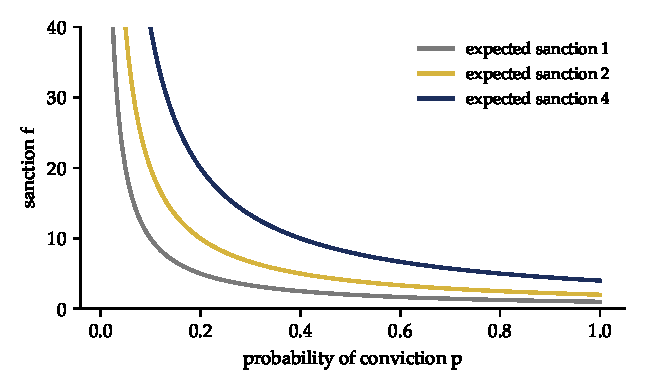
\includegraphics[width=\linewidth]{fig_becker}
\caption{Combinations of the probability of conviction and the sanction that give the same expected sanction. If raising the probability is costly and the sanction is cheap, the efficient point on each curve lies to the left.}
\label{fig:becker}
\end{figure}

\paragraph{Limits} The conclusion is limited by wealth, since fines cannot exceed what the offender can pay; by attitudes to risk, since a risk averse offender is deterred more by severity than by certainty but bears a real cost from an uncertain sanction, while a risk preferring offender is deterred more by certainty than by severity; by the cost of imprisonment when fines are infeasible; and by marginal deterrence, the point, developed by Stigler, that if minor crimes are punished as severely as major ones, offenders have no incentive to stop at the minor crime \citep{stigler1970}. It is also limited by error. Chapter~\ref{ch:standards} showed that the losses from false convictions shape the standard of proof. When sanctions are severe, the loss from a false conviction rises, so the threshold for conviction should rise, which lowers $p$ further for the guilty. Severe sanctions and a high standard of proof interact.\index{marginal deterrence}

\paragraph{Error and deterrence} Errors reduce deterrence. If the probability of conviction for the guilty is $p_G$ and for the innocent is $p_I$, then the difference in expected sanction between offending and not offending is $(p_G - p_I)f$ \citep{kaplow1994}. False convictions of the innocent reduce the deterrent effect of punishment, because they impose sanctions whether or not one offends. Accurate fact finding therefore has deterrent value beyond its fairness value. A more accurate court that reduces $p_I$ while holding $p_G$ fixed increases deterrence at no cost in sanctions.

\section{Enforcers' incentives}

Becker and Stigler extended the analysis to the incentives of those who enforce the law \citep{becker1974}. Police, prosecutors and regulators can be bribed, and an enforcer who takes bribes undermines deterrence. They proposed paying enforcers above market wages, with a bond forfeited on discovery of malfeasance, so that honest service is worth more than a bribe. The analysis applies to the expert witnesses and court officials of earlier chapters: their reports are signals, and their incentives determine the signals' reliability. The selection of favourable experts discussed in Chapter~\ref{ch:fienberg} is a version of the enforcer problem.

\section{The market for illegal goods}

\subsection{Becker, Murphy and Grossman}

In 2006 Becker, Murphy and Grossman analysed the market for illegal goods, using drugs as their example \citep{bmg2006}. Enforcement against suppliers raises their costs: they must evade detection, pay for violence and accept the risk of punishment. Higher costs raise prices and reduce consumption. The question is how much enforcement is optimal, and the answer depends on the elasticity of demand.

Suppose enforcement raises the price of the illegal good. If demand is elastic, with absolute elasticity greater than one, consumption falls proportionately more than price rises, and total spending on the good falls. If demand is inelastic, consumption falls proportionately less, and total spending rises. Since much of the cost of an illegal market is the resources suppliers spend on evasion and violence, and these scale with revenue, enforcement against an inelastically demanded good can increase the social costs of the market while reducing consumption only modestly. Figure~\ref{fig:bmg} shows the sign change at unit elasticity.\index{illegal goods}\index{drugs, market for}

\begin{figure}[t]
\centering
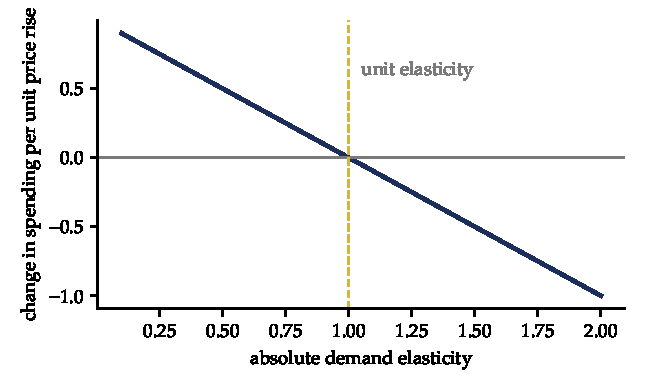
\includegraphics[width=\linewidth]{fig_bmg}
\caption{The change in total spending on an illegal good per unit increase in its price, relative to quantity, as a function of the absolute elasticity of demand. Below unit elasticity, enforcement that raises the price raises total spending.}
\label{fig:bmg}
\end{figure}

Becker, Murphy and Grossman showed that optimal enforcement is lower when demand is less elastic, and that, for goods with inelastic demand, a legal market with a tax could reduce consumption more cheaply than prohibition, because a tax raises the price without inducing the costly evasion and violence that enforcement does. Their analysis did not depend on any particular view of the morality of drug use; it took the reduction of consumption as the goal and asked how to achieve it at least cost.

\subsection{Rational addiction}

Becker and Murphy's earlier theory of rational addiction modelled addictive consumption as a choice by forward looking individuals whose current consumption raises the marginal utility of future consumption \citep{becker1988}. Addicts in the model respond to expected future prices, so permanent price increases reduce consumption more than temporary ones, and announced future enforcement affects current behaviour. Whether addicts are as forward looking as the model assumes is debated, but the empirical evidence that cigarette consumption responds to expected future prices supports at least part of the theory \citep{becker1994}. For legal policy the implication is that the credibility and persistence of enforcement matter: a temporary crackdown has less effect than a durable change.

\subsection{Social interactions}

Becker and Murphy's \emph{Social Economics} studied how individuals' choices depend on those of others through norms, peer effects and social multipliers \citep{becker2000}. Crime is a leading example. Glaeser, Sacerdote and Scheinkman showed that the variance of crime rates across American cities is far larger than individual characteristics can explain, and attributed the excess to social interactions in which one person's offending raises the probability that others offend \citep{glaeser1996}. With social multipliers, a policy that deters some offenders has indirect effects on others, and the total effect of enforcement exceeds its direct effect. Estimation of social multipliers is difficult, because peers' choices are correlated for many reasons, but it is necessary for any honest estimate of the effect of enforcement.

\section{Valuing life and harm}

Damages in tort and the harm from crime must be measured. For injuries to life and health, economists use the value of a statistical life, inferred from the wages workers accept for risky jobs and the prices people pay for safety. Murphy and Topel estimated the social value of improvements in health and longevity in the United States and found them enormous: longevity gains from 1970 to 2000 were worth about 3.2 trillion dollars a year, and the gains of the twentieth century over 1.2 million dollars per person \citep{murphy2006}. The value of a statistical life used by American regulatory agencies is of the order of ten to fourteen million dollars: the Department of Transportation's current figure is about \$14.2 million (base year 2025) \citep{dot2025}. Courts generally do not use these figures directly, but the method, which infers a valuation from choices under risk, is the expected utility approach applied to the measurement of loss.

\section{Punitive damages and the multiplier}

If a defendant who causes harm $H$ is held liable with probability $q < 1$, then compensatory damages of $H$ impose an expected cost of $qH$, less than the harm. The defendant underinvests in care. Polinsky and Shavell argued that punitive damages should make up the difference, so that total damages equal $H/q$: if only one in four injured parties sues and wins, damages should be four times the harm \citep{polinsky1998}. This is Becker's logic applied to tort. It implies that punitive damages should depend on the probability of escaping liability, not on the reprehensibility of the conduct as such, which is the factor American courts emphasise. The Supreme Court in \emph{State Farm v Campbell} suggested that few awards exceeding a single digit ratio between punitive and compensatory damages would satisfy due process \citep{statefarm2003}. In the Polinsky and Shavell framework, a ratio of nine to one corresponds to a probability of liability of one in ten.\index{punitive damages}

\section{The economics of litigation}

\subsection{Why cases settle}

Most civil disputes settle. A trial costs both parties money and time, and if they agreed on the probable outcome they could split the savings. The basic model, due to Landes, Gould (the economist John P. Gould, not the sociologist Roger Gould) and Posner \citep{landes1971,gould1973,posner1973}, says that a case goes to trial only if the parties' expectations diverge enough to overcome the costs. Let the claimant (the plaintiff, in the language of the next subsection) believe it will win with probability $p_P$ and the defendant believe the claimant will win with probability $p_D$. The judgment if the claimant wins is $J$, and the parties' trial costs are $C_P$ and $C_D$. The claimant will accept any settlement above $p_P J - C_P$, and the defendant will pay up to $p_D J + C_D$. Settlement is possible if
\begin{equation}
p_P J - C_P \le p_D J + C_D, \quad\text{that is}\quad (p_P - p_D)\,J \le C_P + C_D .
\label{eq:settle}
\end{equation}
Trials occur when the parties' optimism, $p_P - p_D$, multiplied by the stakes, exceeds the combined costs. Figure~\ref{fig:settlement} shows the settlement zone shrinking as the gap between beliefs grows.\index{settlement}

\begin{figure}[t]
\centering
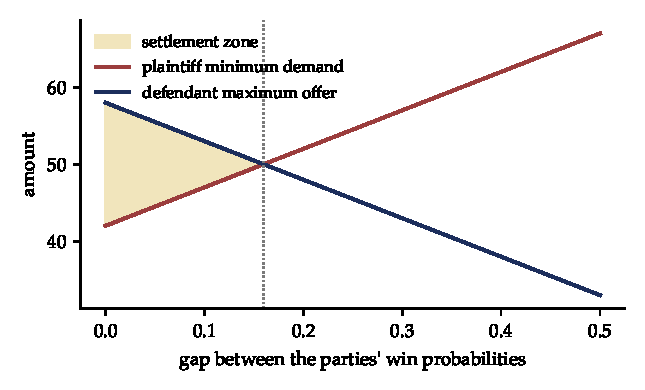
\includegraphics[width=\linewidth]{fig_settlement}
\caption{The claimant's minimum acceptable settlement and the defendant's maximum offer, as functions of the gap between their estimates of the claimant's chance of winning, with stakes of one hundred and costs of eight each. A settlement zone exists only to the left of the dotted line.}
\label{fig:settlement}
\end{figure}

\subsection{Priest and Klein}

Priest and Klein drew a striking implication \citep{priest_klein1984}. If both parties form estimates of the outcome with noise, and cases go to trial only when the estimates diverge, then the cases that are tried are disproportionately those close to the decision standard, where small errors in estimation lead to large disagreements. Cases far from the standard, which one side will clearly win, settle. Among tried cases, plaintiffs should therefore win about half the time, regardless of the underlying distribution of case quality, when the stakes are symmetric. Figure~\ref{fig:priestklein} shows a simulation in which plaintiff win rates at trial approach one half as the noise in the parties' forecasts falls.\index{Priest and Klein}\index{selection of disputes}

\begin{figure}[t]
\centering
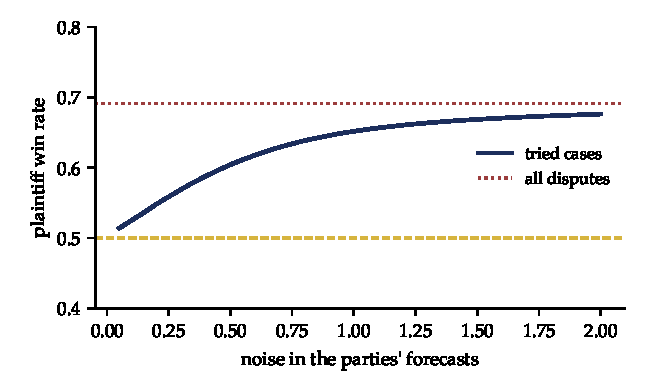
\includegraphics[width=\linewidth]{fig_priest_klein}
\caption{Plaintiff win rate among tried cases as a function of the noise in the parties' forecasts, in a simulation of the Priest and Klein model. Case quality is normal with mean $0.5$ and unit variance, the plaintiff wins if quality is positive, and a case is tried when the parties' estimated win probabilities differ by more than $0.3$, the ratio of combined costs to stakes. Plaintiffs win $69$ per cent of all disputes (dotted line), but the win rate at trial falls toward one half as forecasts become accurate.}
\label{fig:priestklein}
\end{figure}

The Priest and Klein hypothesis has an important implication for any attempt to learn the law from decided cases, including the machine learning approaches of Chapter~\ref{ch:pleadings}. Decided cases are a selected sample of disputes, enriched for close cases. A model trained on them will overestimate how uncertain the law is and will misjudge the outcomes of cases that typically settle. A Bayesian model that represents the selection process explicitly can correct for this; one that ignores it cannot.

\subsection{Asymmetric information}

Bebchuk modelled settlement when one party has private information about the case, in his model the defendant knows the plaintiff's chance of winning and the uninformed plaintiff makes a take-it-or-leave-it demand \citep{bebchuk1984}. The uninformed party makes an offer that some informed types accept and others reject, and trials occur because of the screening, not only because of optimism. In this model trials are a cost of asymmetric information. Discovery reduces asymmetry and so promotes settlement, which is one rationale for broad discovery rules, offset by their cost, as \emph{Twombly} emphasised \citep{twombly2007}.

\subsection{Who pays the costs}

Under the American rule each party bears its own legal costs; under the English rule the loser pays the winner's reasonable costs. The English rule raises the stakes of trial for both sides and makes the outcome matter more. In the optimism model it makes settlement less likely for parties who are both optimistic, because each expects the other to pay its costs, and it deters weak claims, since a claimant with a low probability of success faces paying the defendant's costs. Empirical comparisons are difficult, but the analysis \citep{shavell1982} shows that cost rules are instruments that change the distribution of disputes that reach trial.

\section{Plea bargaining}

In the United States the great majority of criminal convictions result from guilty pleas, typically in exchange for reduced charges or sentences. In a Becker style model, the defendant accepts a plea if the certain sentence $s_{\text{plea}}$ is less than the expected sentence at trial, $\Prob(\text{convict})\,s_{\text{trial}}$, adjusted for risk aversion. The prosecutor offers a plea to economise on trial costs. The problem is that an innocent defendant with a modest probability of conviction may rationally plead guilty if the trial sentence is severe enough. If the probability of wrongful conviction at trial is twenty per cent and the trial sentence is ten years, an innocent defendant who is risk neutral would accept a plea to any sentence below two years.\index{plea bargaining}

A Bayesian view of plea bargaining emphasises that the plea offer reveals information. A prosecutor who offers a large discount signals that her case is weak, and a defendant who rejects a generous offer signals confidence in his innocence or his defence. Grossman and Katz analysed plea bargaining as a screening device that sorts defendants by guilt \citep{grossman1983}. Whether the sorting is good depends on the size of the trial penalty. When the penalty for going to trial is large, the screening breaks down, because innocent and guilty defendants alike plead. Reforms that limit the gap between plea and trial sentences protect the innocent at the cost of more trials.

\section{The cost of the courts}

The Becker framework treats courts as a cost of producing $p$, the probability of conviction. Much of this book has been concerned with reducing that cost or improving the accuracy of what it buys. Chapter~\ref{ch:india} showed what happens when the cost is not met: delay becomes a tax on all litigants and a punishment of the accused. The Bayesian contribution to Becker's program is to model the production of $p$ explicitly, as the result of evidence gathering and inference, so that improvements in inference, such as better forensic statistics, explicit likelihood ratios and machine triage, can be valued in the same units as more police or harsher sentences. A reform that raises the accuracy of verdicts raises deterrence and reduces the harm of false convictions at the same time. That is a strong economic argument for Bayesian courts.

\section*{Notes and Questions}
\addcontentsline{toc}{section}{Notes and Questions}
\begin{enumerate}[label=\arabic*.]
\item In Becker's model with risk neutral offenders, suppose $D(O) = O$, $C(p) = c\,p^2$ with $c = 4$, $O$ is the fraction of the population that offends, fines are costless ($b = 0$) and offenders' gains are uniform on $[0, 10]$. If the maximum fine is $20$, what $p$ minimises social loss?
\item Show that if offenders are risk averse, increasing $f$ while holding $pf$ constant increases deterrence. What does this imply for the optimal mix of $p$ and $f$?
\item In the Becker, Murphy and Grossman analysis, explain why enforcement against a good with inelastic demand can increase the resources devoted to the illegal market.
\item Using \eqref{eq:settle}, with $J = 100$, $C_P = C_D = 10$, find the largest optimism gap at which settlement is possible. How does the English rule change the analysis if the loser pays both parties' costs?
\item A defendant believes there is a thirty per cent chance of conviction at trial, where the sentence would be eight years. What plea offers would a risk neutral defendant accept? How does your answer change if he is risk averse?
\item Explain the Priest and Klein hypothesis in your own words. What does it imply about using appellate decisions to estimate the probability that a type of claim will succeed?
\end{enumerate}

\section*{Further reading}
Becker's 1968 paper \citep{becker1968}; Becker, Murphy and Grossman on illegal goods \citep{bmg2006}; Polinsky and Shavell on public enforcement and on punitive damages \citep{polinsky2000,polinsky1998}; Priest and Klein on the selection of disputes \citep{priest_klein1984}.

\chapter{Antitrust Under Uncertainty}
\label{ch:antitrust}

\section{Predicting harm}

Antitrust law asks courts and agencies to predict. Will this merger raise prices? Did this pattern of prices result from a cartel or from competition? Would this conduct by a dominant firm exclude rivals who would otherwise have competed? The answers depend on counterfactuals that can never be observed: the prices that would have prevailed without the merger, without the agreement, without the conduct. Antitrust is therefore a field of law that leans heavily on statistics, and one in which the Chicago tradition of Becker, Stigler and Posner (Chapter~\ref{ch:becker} treats Becker and Stigler on enforcement) has been influential. This chapter treats antitrust as decision making under uncertainty, examines the statistical methods used to detect cartels, estimate damages and predict merger effects, and argues that a Bayesian framework clarifies both the economics and the law.\index{antitrust}

\section{Error costs}

Frank Easterbrook argued in 1984 that antitrust should be designed with error costs in mind \citep{easterbrook1984}. Courts will sometimes condemn conduct that was in fact procompetitive, false positives, and sometimes permit conduct that was anticompetitive, false negatives. Easterbrook claimed that false positives are more costly, because a mistaken prohibition is enforced by precedent across the economy and persists, while a mistaken permission is eroded by market entry, since monopoly profits attract competitors. He concluded that antitrust rules should be cautious, intervening only where harm is clear.\index{error costs}

This is the decision theory of Chapter~\ref{ch:standards} (the threshold of Equation~\eqref{eq:threshold}) applied to antitrust. The threshold for intervention depends on the ratio of the losses from the two errors. Easterbrook's argument is a claim about that ratio. Critics have argued that conservative error cost reasoning of this kind underestimates the persistence of market power \citep{baker2015}, especially in digital markets with network effects, where entry may not erode dominance for decades. The disagreement is about a ratio of losses and about the prior probability that conduct of a given type is harmful. It can be informed by evidence: studies of the effects of past mergers, of the durability of dominant positions, and of the consequences of past interventions.

\section{Detecting cartels}

\subsection{The problem}

Cartels are secret. Their members agree to fix prices or divide markets, and they conceal their agreements because they are criminal in many jurisdictions. Many cartels are discovered through leniency programmes, which offer immunity to the first member to confess, or through complaints from customers. Statistical screens offer a third route: patterns in prices, bids or market shares that are more probable under collusion than under competition.\index{cartels}

\subsection{Screens as likelihood ratios}

A screen is a statistic computed from market data, with a threshold above which the market is flagged for investigation. Abrantes Metz and colleagues proposed a variance screen: prices under collusion tend to be less variable than under competition, because cartel members avoid price changes that might trigger a price war, so an unusual reduction in price variance is a signal \citep{abrantes2006}. Bid rigging screens look for patterns in procurement auctions: losing bids that are suspiciously close to each other or consistently far above the winning bid (cover bids), rotation of winners, and bidders who never compete in each other's territories.

In Bayesian terms, a screen is a test with a likelihood ratio: the probability of a flag under collusion divided by its probability under competition. As with the polygraph of Chapter~\ref{ch:fienberg}, what a flag implies about a given market depends on the base rate of collusion in the markets screened. If collusion is rare and the screen's false positive rate is not tiny, most flags will be false. Screens are useful for directing investigative resources, not for proving guilt. A flagged market should be investigated, and the investigation should look for evidence with much larger likelihood ratios, such as communications between competitors.

\subsection{LIBOR}

The London Interbank Offered Rate was set by a trimmed average of the rates at which panel banks reported they could borrow. In 2008 journalists, notably in a Wall Street Journal article of 29 May 2008, noted that some banks' submissions seemed implausibly low relative to other measures of their credit risk, such as credit default swap spreads. Statistical work found some anomalous individual submissions but concluded that the evidence was inconsistent with a material manipulation of one month dollar LIBOR, and that statistical methods alone do not prove manipulation \citep{abrantes2012}. Regulatory investigations later established that traders at several banks had sought to manipulate submissions for profit, and that during the financial crisis some banks had submitted low rates to appear healthier. Banks paid billions in fines, and several traders were prosecuted, with mixed results on appeal. The statistical evidence was an early signal; the decisive evidence was messages between traders and submitters, whose likelihood ratio for manipulation was overwhelming.

\section{Damages}

\subsection{The overcharge}

A purchaser injured by a cartel can recover damages equal to the overcharge: the difference between the price paid and the price that would have prevailed without the cartel, multiplied by the quantity purchased. In the United States, damages are trebled. Estimating the counterfactual price is the central problem. Common methods compare prices before, during and after the cartel period; compare prices in the cartelised market with prices in a similar market that was not cartelised, the yardstick method; and fit a regression of prices on cost and demand variables with an indicator for the cartel period.\index{overcharge}

Each method produces an estimate with uncertainty, and each depends on assumptions: that nothing else changed when the cartel began and ended, that the yardstick market is comparable, that the regression captures the determinants of price. A Bayesian approach combines the methods, weighting each by its credibility, and reports a posterior distribution for the overcharge. Where the methods disagree, a model that allows each method its own bias gives a wide posterior, which is a fact the court should know; simple precision weighting, which assumes every method is unbiased, does not.

\subsection{Class certification}

In \emph{Comcast Corp v Behrend} the Supreme Court held in 2013 that a plaintiff seeking class certification must show that damages are capable of measurement on a class wide basis, and that the damages model must measure only the damages attributable to the theory of liability accepted for class action treatment \citep{comcast2013}. The plaintiffs' expert had estimated damages from four theories of antitrust impact, but only one had been accepted, and his model did not separate its effect. The case illustrates a general point: a damages model must correspond to the causal structure of the claim. In the language of Chapter~\ref{ch:graphs}, the model must estimate the effect of the specific intervention alleged, not a combination of effects.

\subsection{Pass on}

When a direct purchaser passes some of the overcharge on to its own customers, who has been injured? In the United States, \emph{Illinois Brick} held that indirect purchasers generally cannot recover under federal law, and \emph{Hanover Shoe} that defendants cannot reduce direct purchasers' damages by showing pass on. In the United Kingdom and the European Union, pass on is a defence and indirect purchasers can sue. The Supreme Court of the United Kingdom considered the issues in the interchange fee litigation against card schemes. The estimation of pass on rates is another counterfactual exercise, and the Bayesian approach of combining evidence with stated uncertainty applies.

\section{Mergers}

\subsection{The prediction problem}

Merger control requires agencies to predict, before a merger, whether it will substantially lessen competition. The prediction is made under uncertainty about demand, costs, the response of rivals and the likelihood of entry. Agencies in the United States, the United Kingdom and the European Union use a combination of market definition, measures of concentration, and direct predictions of price effects.

\subsection{Market definition and the hypothetical monopolist}

Market definition asks what products and areas constrain the merging firms' prices. The hypothetical monopolist test asks whether a hypothetical monopolist of a candidate set of products could profitably impose a small but significant and non transitory increase in price, conventionally five or ten per cent. If so, the set is a relevant market; if not, it must be widened. The test is a thought experiment that requires estimates of demand elasticities and margins, and its answer is uncertain when those estimates are.

\subsection{Upward pricing pressure}

Farrell and Shapiro proposed upward pricing pressure as an alternative to market definition for differentiated products \citep{farrell2010}. When two firms merge, each firm's price increase diverts some customers to the other, whose sales now benefit the merged firm. The incentive to raise price depends on the diversion ratio, the fraction of lost sales captured by the partner, and on the partner's margin. For firm 1, upward pricing pressure is $\mathrm{UPP}_1 = D_{12}(P_2 - C_2) - E_1 C_1$, where $D_{12}$ is the diversion ratio from firm 1 to firm 2, $P_2 - C_2$ is the partner's margin in money terms, and $E_1$ is the efficiency gain expressed as a fraction of firm 1's marginal cost $C_1$. Gross upward pricing pressure, GUPPI, is the first term alone divided by firm 1's price, $D_{12}(P_2 - C_2)/P_1$, the pressure before any efficiency credit. Upward pricing pressure is positive when the value of diverted sales exceeds the efficiency gain. The measure uses quantities that can be estimated from data on customer switching and from margins, and it avoids the binary choice of market definition.

\subsection{Merger simulation and Bayesian demand}

Merger simulation goes further: it estimates a model of demand and supply, simulates the post merger equilibrium, and predicts price changes. The standard demand model for differentiated products is the random coefficients logit model of Berry, Levinsohn and Pakes \citep{blp1995}, which allows consumers to differ in their tastes and so produces realistic substitution patterns. Estimating it is demanding, and estimates can be sensitive to choices of instruments and specification.

Bayesian estimation of such models, as in the work of Jiang, Manchanda and Rossi \citep{jiang2009} and in our own work on a Bayesian version of the Berry, Levinsohn and Pakes framework for antitrust \citep{polson_sokolov_blp}, produces a posterior distribution for the demand parameters and therefore for the predicted price effects of a merger. Instead of a single predicted price increase, the agency obtains a distribution: the probability that prices rise by more than five per cent, the probability that they fall. This is exactly what the decision requires. If the agency's losses from blocking a beneficial merger and from clearing a harmful one are known, the optimal decision is the one that minimises expected loss under the posterior, as in Chapter~\ref{ch:standards}. Bayesian merger simulation can turn the substantial lessening of competition test into an explicit decision rule once the losses are stated.\index{merger simulation}\index{Berry Levinsohn Pakes}

\begin{keybox}
A merger decision as a Bayesian problem. Let $\Delta$ be the post merger change in average price. The agency's posterior for $\Delta$ comes from a demand model estimated with Bayesian methods. Let $L_B(\Delta)$ be the loss from blocking, which is large if $\Delta$ is negative because consumers lose efficiencies, and $L_C(\Delta)$ the loss from clearing, which is large if $\Delta$ is positive. Block if $\E[L_C(\Delta)] > \E[L_B(\Delta)]$ under the posterior. Uncertainty about $\Delta$ enters directly, rather than being replaced by a single point prediction.
\end{keybox}

\subsection{Retrospectives}

The most useful evidence for setting priors in merger control comes from retrospective studies of past mergers, which compare post merger prices with what a control group suggests would have happened. Such studies have found that a meaningful share of mergers that were cleared led to price increases, which suggests that agencies' priors or thresholds may have been too permissive in some industries. A Bayesian agency would use retrospective evidence to update its priors on the effects of mergers of different types, in a hierarchical model across industries.

\section{Dominance in digital markets}

The largest antitrust cases of the 2020s have concerned digital platforms. In the United States, the government's case against Google over search distribution led a federal court in 2024 to find that Google had unlawfully maintained a monopoly in general search, with remedies decided in September 2025 that stopped short of requiring divestiture of the Chrome browser, barred exclusive distribution contracts, and required Google to share certain search data with rivals. In the United Kingdom, the Competition and Markets Authority's review of Microsoft's acquisition of Activision Blizzard initially blocked the deal on cloud gaming grounds in 2023, then cleared a restructured transaction in which cloud streaming rights were sold to a third party. The European Union's Digital Markets Act imposes ex ante obligations on designated gatekeepers rather than relying on case by case enforcement.

These cases raise in acute form the question of error costs. If dominance in digital markets is durable because of network effects and data advantages, false negatives are more costly than Easterbrook supposed. If digital markets are dynamic and today's dominant firm can be displaced by a new technology, intervention risks false positives. The arrival of generative AI, which has created new competition in search and threatens to reshape several platforms, is a test case for this question. A Bayesian approach would treat the durability of dominance as an uncertain parameter, update it with evidence from such episodes, and let the posterior inform the threshold for intervention.

\section*{Notes and Questions}
\addcontentsline{toc}{section}{Notes and Questions}
\begin{enumerate}[label=\arabic*.]
\item A variance screen flags ten per cent of competitive markets and sixty per cent of cartelised ones. If one market in fifty is cartelised, what fraction of flagged markets are cartelised?
\item Three methods estimate a cartel overcharge at eight, twelve and twenty per cent, with standard errors of three, four and eight per cent. Combine them by precision weighting. What does the spread of the estimates suggest about the assumptions?
\item Explain the holding in \emph{Comcast Corp v Behrend} in terms of the causal structure of a damages model.
\item Two merging firms have equal prices, a diversion ratio of thirty per cent from each to the other and margins of forty per cent. Compute the gross upward pricing pressure as a fraction of price. What efficiency gain would offset it?
\item Formulate the merger decision as in the keybox with a posterior for $\Delta$ that is normal with mean two per cent and standard deviation three per cent, and losses linear in $\Delta$ on each side, with slopes $c_C$ for clearing and $c_B$ for blocking. For what ratio $c_C/c_B$ should the agency block?
\item Easterbrook argued that false positives are costlier than false negatives in antitrust. What evidence would you collect to test this claim for digital markets?
\end{enumerate}

\section*{Further reading}
Easterbrook on the limits of antitrust \citep{easterbrook1984}; Farrell and Shapiro on upward pricing pressure \citep{farrell2010}; Berry, Levinsohn and Pakes \citep{blp1995}; Jiang, Manchanda and Rossi on Bayesian random coefficients logit \citep{jiang2009}; Abrantes Metz and colleagues on the variance screen \citep{abrantes2006}; our Bayesian version of the Berry, Levinsohn and Pakes framework \citep{polson_sokolov_blp}.

\chapter{Judges, Costs and the Justice System}
\label{ch:systemcosts}

\section{Justice is a scarce resource}

Courts cost money. Judges are paid, court buildings maintained, staff employed, records kept. Parties pay lawyers and experts, and they and their witnesses give up time. Delay imposes further costs: a claimant waiting for compensation, a business with capital tied up, an accused person on remand. Every hour a judge spends on one case is an hour not spent on another. A legal system is therefore an allocation problem: how to spend limited resources to produce the most justice. This chapter applies the decision theory of Chapter~\ref{ch:decisions} to that problem. It asks how much accuracy is worth, how judges' time should be allocated, what appeals are for, and how the rules on legal costs shape the cases that reach court.\index{costs of justice}

\section{The value of accuracy}

\subsection{Kaplow's question}

Louis Kaplow asked why the legal system should value accuracy at all \citep{kaplow1994}. On Kaplow's view, accuracy in adjudication has no value in itself; its value lies in its effects. Accurate determinations of liability improve incentives, because people who know they will be held liable only if they cause harm, and will be held liable if they do, take appropriate care. Accurate determinations of damages improve incentives in the same way. Accuracy also matters for fairness and for the legitimacy of the courts. But each of these benefits has limits, and accuracy is costly. The optimal level of accuracy balances its marginal benefit against its marginal cost.\index{Kaplow, Louis}\index{accuracy, value of}

\subsection{The trade off}

Figure~\ref{fig:accuracy} shows the trade off for a single case. As resources devoted to the case increase, the cost of process rises and the expected cost of errors falls, quickly at first and then more slowly. Total cost is minimised where the marginal cost of process equals the marginal reduction in error cost. The optimum depends on the stakes. A case where an error would cost a great deal (a murder trial, a dispute over a large business) justifies more process; a small claim justifies less. This is why legal systems have tracks: small claims procedures, fast, intermediate and multi tracks in England, magistrates' courts and the Crown Court, summary and plenary procedures elsewhere. Each track is a point on the trade off appropriate to a class of cases.

\begin{figure}[t]
\centering
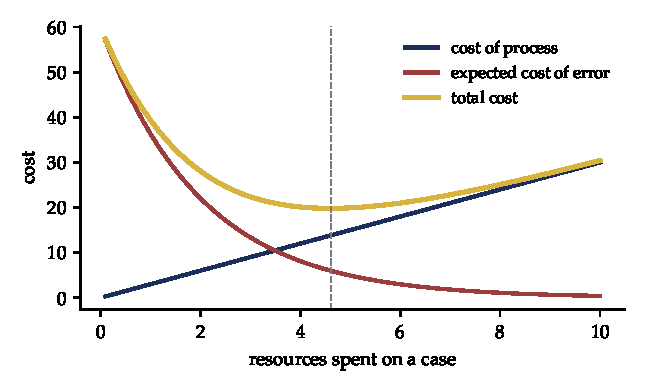
\includegraphics[width=\linewidth]{fig_accuracy}
\caption{The cost of process, the expected cost of error and their sum, as functions of the resources spent on a case. The dashed line marks the optimum. Illustrative.}
\label{fig:accuracy}
\end{figure}

\subsection{Accuracy about what?}

Kaplow emphasised that the value of accuracy differs across issues. Accuracy about whether a defendant was negligent matters for incentives because it determines whether careless people pay; accuracy about the exact amount of damages matters less if errors are unbiased, since risk-neutral potential defendants care about expected liability, and matters only to the extent that they can foresee the harm they might cause when choosing precautions \citep{kaplowshavell1996}. Courts might therefore spend more on liability and less on quantum, or use rough schedules for damages in routine cases, such as the tariffs for injuries in the Judicial College guidelines in England, while reserving full assessment for large claims.

\section{Allocating judges' time}

\subsection{The docket as a portfolio}

A judge or a court has a docket of cases and a fixed amount of time. Each case would benefit from more time, in the sense of a lower expected error cost, but the benefit varies. The efficient allocation gives each case time until the marginal reduction in expected error cost per hour is equal across cases. Cases near the decision threshold, where the posterior is close to the standard of proof, benefit most from additional evidence and argument, as the value of information analysis of Chapter~\ref{ch:standards} showed. Cases far from the threshold benefit little and can be decided quickly.\index{docket management}

This principle supports active case management. Under the Civil Procedure Rules introduced after Lord Woolf's reforms, English courts must seek to give effect to the overriding objective\index{overriding objective} of dealing with cases justly and at proportionate cost, including by allotting to each case an appropriate share of the court's resources while taking into account the need to allot resources to other cases. The phrase is a statement of the allocation principle. A Bayesian approach would make it operational, by estimating for each case the probability of each outcome and the value of further process, and allocating time accordingly.

\subsection{Judges as a cost of the system}

Judges' time is the scarcest resource in most court systems. In England and Wales, shortages of judges and recorders have contributed to large backlogs in the Crown Court, with some trials listed long after charge. In India, as Chapter~\ref{ch:india} showed, the judge to population ratio is a fraction of what the Law Commission recommended. In the United States, judicial vacancies and rising caseloads have lengthened federal civil dockets. The marginal value of an additional judge is the value of the cases that judge would decide, plus the reduction in delay for all cases. Where delay is long, that value is large: each year of delay for a remanded defendant costs the defendant their liberty and the state the cost of custody, and each year of delay in a civil case reduces the value of the claim and of the incentive the law provides.

\subsection{The cost of delay}

The cost of delay can be estimated. For a civil claim of value $J$ with probability of success $p$, a delay of $t$ years at a discount rate $r$ reduces the present value of the expected recovery from $pJ$ to $pJ e^{-rt}$, and if interest awarded does not fully compensate for delay, the claimant bears the difference. Delay also reduces accuracy, as memories fade and evidence is lost, which raises the expected error cost. For a remanded defendant, the cost is the value of liberty lost, which the law recognises by crediting time on remand against any sentence, but which is not compensated if the defendant is acquitted. In a system with long delays, these costs can dwarf the direct costs of courts.

\section{Appeals as error correction}

Steven Shavell analysed appeals as a means of correcting errors \citep{shavell1995}. If trial courts make errors and appellate courts can detect some of them, an appeal system reduces the expected error cost at the price of appellate resources and further delay. Appeals are efficient when the parties who appeal are disproportionately those who suffered errors, so that the appellate courts' resources are concentrated on the cases most likely to be wrong. Parties have private information about whether the trial court erred, and the cost of appealing deters those with weak grounds; the appeal process works as a screen.\index{appeals}

In Bayesian terms, the decision to appeal is a decision under uncertainty about the appellate outcome, and the permission stage, which requires a real prospect of success or some other compelling reason in England, is a threshold on that probability. Permission to appeal economises on appellate time by excluding appeals with low posterior probability of success. The threshold should depend on the stakes and on the value of the appeal for clarifying the law, since appellate decisions are public goods that guide future cases. A case with a modest probability of success but a large question of law may warrant permission because of its value as precedent, a benefit that accrues to people other than the parties.

\section{Who pays: costs rules}

\subsection{The English and American rules}

Under the English rule the losing party pays the winner's reasonable costs, assessed by the court. Under the American rule each party bears its own costs, subject to exceptions. Chapter~\ref{ch:becker} discussed how these rules affect settlement. Here we consider their effect on access and on the composition of cases. The English rule raises the stakes of litigation, deterring claims with a low probability of success, since a losing claimant pays two sets of costs, and encouraging claims with a high probability, since a winning claimant recovers most of its costs. The American rule makes small claims with a high probability of success uneconomic, since the claimant's costs eat into the recovery, and allows weak claims with large stakes to be brought, since the defendant cannot recover its costs.\index{costs rules}

\subsection{Proportionality and costs management}

In England, Lord Justice Jackson's review of civil litigation costs led to reforms in 2013 that made proportionality a central test for recoverable costs, introduced costs budgeting, under which the court approves each party's budget in advance, and changed the rules on conditional fee agreements and after the event insurance. From October 2023 fixed recoverable costs\index{fixed recoverable costs} were extended to most civil claims of up to one hundred thousand pounds. These reforms implement the principle that the cost of process should be proportionate to what is at stake, the principle illustrated in Figure~\ref{fig:accuracy}.

Fixed costs trade accuracy for predictability. A party knows in advance what it will recover or pay if it wins or loses, which makes the expected value calculations of Chapter~\ref{ch:decisions} easier and settlement more likely. The cost is that cases requiring more work than the fixed amount allows may be under resourced. The decision theoretic view supports fixed costs for routine cases with predictable demands and budgeted costs for complex ones, the structure the English reforms adopted.

\subsection{Legal aid}

When one party cannot afford representation, the adversarial system of Chapter~\ref{ch:commoncivil} loses its main safeguard: the fact finder hears only one side's evidence searched with vigour. Legal aid, by funding representation, restores the competition between information gatherers that makes adversarial procedure work. Cuts to civil legal aid\index{legal aid} in England under the Legal Aid, Sentencing and Punishment of Offenders Act 2012 led to a large increase in litigants in person, notably in family cases, who may take more court time per case and may be less able to present meritorious claims. The decision theoretic analysis suggests that the savings from legal aid cuts should be weighed against the increased error cost and the increased cost of court time, both of which fall on the system.

\section{Measuring the system}

A court system that wants to allocate resources well needs data: the number and type of cases, their duration, outcomes, appeals and reversals, and costs. Reversal rates on appeal are a rough measure of error, though they understate it, since most errors are not appealed and appellate courts defer to trial courts on findings of fact and reverse them only for clear error. Delay statistics measure one cost. Surveys of court users measure perceived fairness. The Indian National Judicial Data Grid of Chapter~\ref{ch:india} shows what public data on a court system can look like. A Bayesian court administrator would use such data to estimate the value of information and the cost of delay by case type, and allocate judges, courtrooms and support accordingly.

\section{Judges as decision makers}

Finally, judges are themselves decision makers with objectives and constraints. They seek to decide correctly, to avoid reversal, to manage their dockets, and in many systems to advance in their careers. Their incentives shape their decisions. Richard Posner, a judge as well as a scholar, wrote about judges as economic actors who maximise a utility that includes leisure, reputation and the satisfaction of deciding well. Research has documented effects of caseload pressure on decisions, and the noise between judges to which Chapter~\ref{ch:hume} returns. A system that measures judges' performance risks distorting it, as France feared when it banned judge analytics (Chapter~\ref{ch:commoncivil}); a system that does not measure it cannot improve it. The Bayesian response is to measure error and delay at the level of the court and the case type, where the purpose is allocation and reform, and to protect individual judges' independence in deciding the merits.

\section*{Notes and Questions}
\addcontentsline{toc}{section}{Notes and Questions}
\begin{enumerate}[label=\arabic*.]
\item In Figure~\ref{fig:accuracy}, the cost of process is $3e$ and the expected error cost $60e^{-0.5e}$. Find the optimal $e$. How does it change if the stakes, and hence the error cost, double?
\item A court has two kinds of case: those with posterior near one half, where an hour of hearing reduces expected error cost by ten units, and those with posterior near zero or one, where it reduces it by one unit. How should a judge with ten hours allocate time between five cases of each kind?
\item Compute the present value lost by a claimant with a fifty per cent chance of recovering one hundred thousand pounds if trial is delayed by two years at a discount rate of five per cent (continuous compounding) and interest is awarded at two per cent.
\item Explain Shavell's argument that appeals can be an inexpensive way to correct errors, because litigants' private knowledge of whether the trial court erred screens which cases reach the appellate court.
\item Under fixed recoverable costs, a claimant knows it will recover a fixed sum if it wins. How does this change the decision whether to sue, compared with assessed costs?
\item Should a court system publish statistics on the reversal rates of individual judges? Weigh the value of the information against its costs.
\end{enumerate}

\section*{Further reading}
Kaplow on the value of accuracy \citep{kaplow1994}; Shavell on appeals \citep{shavell1995}; and the reports of Lord Woolf and Lord Justice Jackson on civil justice in England and Wales.

\chapter{Litigation Funding, Class Actions and Claims as Assets}
\label{ch:funding}

\section{Claims are assets}

A legal claim is a risky asset. Its owner holds a right to a payment that will be made only if the claim succeeds, after a delay, net of costs. Like any risky asset it has an expected value, a variance and a correlation with other assets, and it can be bought, sold, financed and insured. For most of the history of the common law, the doctrines of maintenance and champerty forbade strangers from funding litigation in return for a share of the proceeds, on the ground that it encouraged speculative and oppressive suits. Those doctrines have been relaxed or abolished in most of the common law world, and third party litigation funding is now an industry measured in billions. This chapter applies the decision theory of this book to the funding, aggregation and valuation of claims, which are among the most important developments in modern litigation.\index{litigation funding}

\section{Valuing a claim}

The expected value of a claim to its owner is
\begin{equation}
V = \sum_k \Prob(\text{outcome } k)\,\big(\text{recovery}_k - \text{costs}_k\big)\,e^{-r t_k},
\end{equation}
summed over the possible outcomes, including settlement at various stages, judgment for the claimant at various amounts, and judgment for the defendant. The probabilities come from the analysis of issues described in Chapters~\ref{ch:pleadings} and~\ref{ch:pleadingscases}; the recoveries from the damages analysis of Chapter~\ref{ch:damages}; the costs from the rules of Chapter~\ref{ch:systemcosts}; and the timings from the court's calendar. Each input is uncertain, and a Bayesian valuation reports a distribution, not a number.

\section{The funder's decision}

\subsection{A single claim}

A funder that pays a claimant's costs in exchange for a share of the recovery faces a bet. If the claim succeeds, the funder typically receives historically a multiple of its investment or a percentage of the damages, whichever is greater; if it fails, the funder loses its investment and, under the English costs rule, may be liable for the defendant's costs, usually covered by after the event insurance\index{after the event insurance}. With probability of success $p$, return multiple $m$ on success and loss of the stake on failure, the expected return per unit invested is $pm - 1$. A funder requiring an expected return of fifty per cent over the life of the claim on a claim with a sixty per cent chance needs $m \ge 2.5$. In the net odds $b = m - 1$ of the Kelly example below, the portfolio example ($m = 3$) and the Kelly example ($b = 2$) are the same claim.

\subsection{Portfolios}

A single claim is a highly risky asset: the funder either multiplies its money or loses it all. Funders reduce risk by holding portfolios of claims whose outcomes are not strongly correlated. Figure~\ref{fig:funding} shows the distribution of returns for a funder holding one, five and twenty independent claims, each with a sixty per cent chance of returning three times the stake. The expected return is the same; the variance falls with the number of claims. A funder with twenty independent claims almost never loses money overall. Correlation matters: claims against the same defendant, or turning on the same question of law, can fail together, and a portfolio built from them is riskier than its size suggests.\index{portfolio of claims}

\begin{figure}[t]
\centering
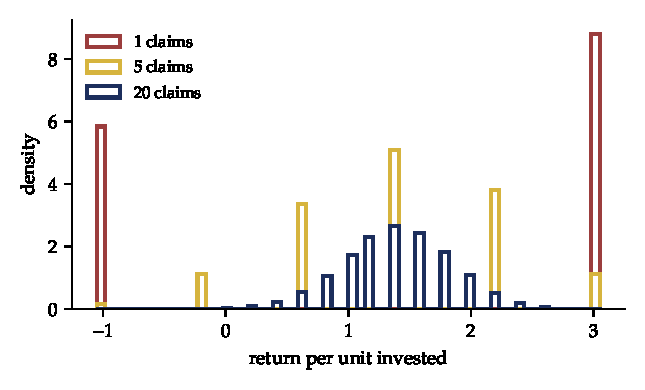
\includegraphics[width=\linewidth]{fig_funding}
\caption{Simulated return per unit invested for a funder holding one, five and twenty independent claims, each succeeding with probability $0.6$ and returning three times the stake. Diversification narrows the distribution without changing its mean.}
\label{fig:funding}
\end{figure}

\subsection{How much to invest}

How much of its capital should a funder commit to a single claim? The Kelly criterion, which maximises the expected logarithm of wealth and so the long run growth rate, gives the answer for a sequence of independent bets: invest a fraction
\begin{equation}
f^\ast = \frac{p\,b - (1-p)}{b}
\end{equation}
of capital, where $b$ is the net odds, the profit per unit staked on success. With $p = 0.6$ and $b = 2$, the Kelly fraction is $0.4$. This is the criterion of \citet{kelly1956}. In practice funders bet much less than the full Kelly fraction, because their estimates of $p$ are optimistic and overestimating $p$ leads to overbetting, which lowers long run growth and can make it negative, because their utility is more risk averse than the logarithm, and because they face limits on drawdowns. Fractional Kelly betting is the standard response \citep{maclean2011}. Posterior uncertainty about $p$ does not by itself reduce the fraction: expected log wealth is linear in $p$, so only the posterior mean of $p$ enters, and the optimal fraction is the Kelly fraction at that mean.\index{Kelly criterion}

\section{The law of funding}

\subsection{England after PACCAR}

In \emph{R (PACCAR Inc) v Competition Appeal Tribunal} the Supreme Court held in 2023 that litigation funding agreements under which the funder's return was calculated as a percentage of damages were damages based agreements within the meaning of the statute regulating them, and so were unenforceable unless they complied with the regulations, which most did not \citep{paccar2023}. The decision threatened the enforceability of a large number of existing agreements, particularly in collective proceedings in the Competition Appeal Tribunal. Funders restructured their agreements to calculate returns as multiples of the investment, and the Civil Justice Council recommended legislation to reverse the effect of the decision and to introduce light touch regulation of funding.\index{PACCAR}

\subsection{Funder control and conflicts}

Funding raises conflicts. The funder's interest is in the expected value of its return; the claimant's is in its own recovery. They may disagree about whether to settle. A funder with a large return multiple may prefer to reject a settlement that would leave little after its share, even if the settlement is in the claimant's interest. The decision theoretic analysis makes the conflict explicit: the funder's expected utility and the claimant's expected utility are different functions of the same settlement offer, and their preferred thresholds for acceptance differ. Agreements, regulation and the courts must allocate control.

\begin{casebox}{The Post Office litigation}
In \emph{Bates v Post Office}, to which Chapter~\ref{ch:lean} returns, a group of hundreds of sub postmasters, funded by a litigation funder, sued the Post Office over the Horizon accounting system \citep{bates2019}. After the claimants won the Common Issues judgment in 2019 \citep{bates2019common}, the case settled for about fifty eight million pounds. Most of the settlement went to the funder and the lawyers, leaving the claimants a small fraction, and the government later established compensation schemes that paid far more. The case showed both the value of funding, without which the litigation could not have been brought against a well resourced defendant, and the problem of distribution, when the costs of a long case consume most of its proceeds.
\end{casebox}

\section{Class and collective actions}

\subsection{Aggregation}

Many wrongs cause small losses to many people: overcharges from a cartel, misleading fees, data breaches. Individually, the claims are too small to litigate. Aggregated, they are large. Class actions in the United States under Rule 23 of the Federal Rules of Civil Procedure, and collective proceedings in the Competition Appeal Tribunal under the Competition Act 1998 as amended by the Consumer Rights Act 2015, allow a representative to sue on behalf of a class. On an opt out basis, the class includes everyone affected unless they choose to leave.\index{class actions}\index{collective proceedings}

\subsection{Merricks v Mastercard}

The largest UK collective action, brought by Walter Merricks on behalf of some forty six million consumers, alleged that Mastercard's interchange fees had raised the prices of goods. Its certification was the subject of a Supreme Court decision in 2020 that set a relatively low bar for certification and recognised that the tribunal could estimate aggregate damages\index{aggregate damages} without assessing each class member's loss \citep{merricks2020}. The claim was eventually settled for two hundred million pounds, far below the original claim of about fourteen billion, and the tribunal approved the settlement over the objection of the funder, which argued that it was too low.

The case illustrates the decision problems of collective actions. The class representative must decide whether to settle on behalf of millions of absent class members who cannot be consulted. The tribunal must decide whether the settlement is fair, which requires it to estimate the expected value of continuing, including the probability of success on liability, the distribution of damages, the time to judgment and the costs. And the distribution of the settlement between class members, funder and lawyers must be decided, which requires a view of the funder's risk and the reasonable return on it. Each of these is a Bayesian decision, made explicit or not.

\subsection{Aggregate damages}

Aggregate damages, estimated for the class as a whole rather than for each member, are a natural application of the posterior mean of Chapter~\ref{ch:damages}. If the overcharge per transaction has a posterior distribution and the number of transactions is known, the expected aggregate loss is the number of transactions times the posterior mean overcharge, and its uncertainty can be computed. The defendant is liable for the expected harm caused, which gives the right incentives, while individual class members receive a share that may differ from their individual loss. The trade off between accuracy for individuals and feasibility for the class is the trade off of Chapter~\ref{ch:systemcosts} at the scale of millions.

\section{Claims in sovereign and commercial disputes}

Funding is now common in international arbitration and in claims against states. The most prominent example is the litigation over Argentina's expropriation of the oil company YPF, in which a funder acquired the claims of former shareholders and a federal court in New York entered a judgment of more than sixteen billion dollars against Argentina in 2023, which the Second Circuit reversed on appeal in 2026, with further review sought. Such claims have very skewed payoff distributions: a small probability of a very large recovery, uncertain timing and the risk that a judgment cannot be enforced against a sovereign. Their valuation requires probabilities for each stage, liability, quantum, appeal and enforcement, and markets in which such claims are traded reveal investors' posteriors on them.

\section{Insurance and the pricing of legal risk}

After the event insurance covers a claimant's liability for the defendant's costs if the claim fails, and its premium is a price for legal risk. Insurers price it from their estimate of the probability of failure and the expected adverse costs. Judgment preservation insurance, a newer product, insures a judgment against reversal on appeal. These markets are informative: an insurer that will underwrite a judgment against reversal at a low premium has assessed a low probability of reversal. A Bayesian court administrator, or an academic studying courts, can learn from these prices, as from market prices in Chapter~\ref{ch:securities}.

\section{Policy}

The decision theory of this book supports three conclusions about funding and aggregation. First, funding improves access to justice when the claimant's alternative is not to sue at all, because it transfers risk to a party better able to bear it through diversification. Second, the terms of funding should be transparent to the court, which must be able to assess whether a settlement serves the class or the funder. Third, aggregate procedures are justified when the cost of individual adjudication exceeds the value of individual accuracy, the trade off of Chapter~\ref{ch:systemcosts} applied to the class. Each conclusion can be made quantitative with the tools of this book, and courts approving settlements and funding arrangements would benefit from doing so.

\section*{Notes and Questions}
\addcontentsline{toc}{section}{Notes and Questions}
\begin{enumerate}[label=\arabic*.]
\item A claim has a fifty five per cent chance of success, a recovery of ten million if successful, costs of two million and a duration of three years. At a discount rate of eight per cent, what is its expected present value, taking the costs as paid when the claim resolves? What return multiple must a funder receive to earn twenty per cent a year?
\item For a funder holding twenty claims, each with $p = 0.6$ and a return of three times the stake, compute the probability of losing money overall if the claims are independent. Repeat with pairwise correlation $0.3$.
\item Compute the Kelly fraction for $p = 0.55$ and net odds of two. If the posterior for $p$ is uniform between $0.45$ and $0.65$, what fraction maximises expected log wealth?
\item Explain the conflict between funder and claimant over a settlement offer, using expected utility for each. How should a court approving a collective settlement resolve it?
\item In \emph{Merricks}, the claim was for about fourteen billion and the settlement two hundred million. What probability of success and expected damages would make that settlement fair, allowing for costs and delay?
\item Should litigation funding be regulated? Frame your answer in terms of the information the court needs and the incentives of funders.
\end{enumerate}

\section*{Further reading}
\emph{PACCAR} \citep{paccar2023}; \emph{Merricks v Mastercard} \citep{merricks2020}; and, on Kelly betting, \citet{kelly1956} and \citet{maclean2011}.

\chapter{Sentencing, Bail and Parole as Decisions}
\label{ch:sentencing}

\section{After the verdict}

A conviction is not the end of the decisions a criminal justice system makes about a person. Before trial, a court decides whether to release or detain. After conviction, it chooses a sentence. During custody, a parole board decides whether to release early. After release, probation officers decide whether to recall. Each decision is made under uncertainty about the person's future conduct, and each has costs on both sides: the cost of detention to the person, their family and the state, and the cost to potential victims of release. These are the clearest examples in law of decisions with explicit Type I and Type II errors, and they are where risk assessment\index{risk assessment} tools and machine learning have entered the courts most directly. This chapter applies the framework of Chapter~\ref{ch:decisions}.\index{sentencing}\index{parole}

\section{Objectives of sentencing}

Sentencing serves several purposes. Section 57 of the Sentencing Act 2020 in England and Wales lists them: the punishment of offenders, the reduction of crime including by deterrence, the reform and rehabilitation of offenders, the protection of the public, and the making of reparation. American statutes list similar purposes. These objectives conflict. Punishment proportional to culpability may be shorter or longer than protection of the public requires; rehabilitation may be better served in the community than in custody; whether deterrence depends more on the certainty or the severity of punishment turns on the offender's attitude to risk, as Chapter~\ref{ch:becker} discussed.\index{objectives}

Decision theory does not resolve these conflicts, which are matters of value. It makes them explicit by asking the sentencer to state the loss from each outcome. A sentence that is too lenient, relative to culpability, imposes a loss on the value of proportionate punishment; one that is too severe imposes a loss on the offender and the state. A sentence that releases a dangerous offender too soon imposes a loss on future victims; one that holds a person who would not reoffend imposes a loss on that person. Separating the retributive component, which depends on the offence, from the incapacitative component, which depends on predicted risk, clarifies which decisions turn on probabilities and which do not.

\section{Guidelines as decision rules}

In England and Wales, courts must follow sentencing guidelines issued by the Sentencing Council unless it would be contrary to the interests of justice to do so. The guidelines specify categories of harm and culpability, starting points and ranges, and aggravating and mitigating factors. In the United States, the federal Sentencing Guidelines were mandatory until \emph{United States v Booker} made them advisory in 2005 \citep{booker2005}. Guidelines are decision rules: they map features of the case to a recommended action. Their purpose is to reduce noise, the unwarranted variation between sentencers that Chapter~\ref{ch:hume} examines, while preserving the sentencer's ability to depart in unusual cases.\index{sentencing guidelines}

A Bayesian view of guidelines treats them as priors: the guideline range is the default, and the sentencer departs when the specific facts provide strong enough evidence that the default is wrong for this case. This is one way to read the English statutory test. It also suggests how guidelines should be revised: by comparing outcomes, such as reoffending, across sentences for similar cases, and updating the guideline when the evidence shows that a different sentence would better serve the purposes.

\section{Bail}

\subsection{The decision}

Chapter~\ref{ch:decisions} worked a bail example: release if the probability of failure $r$ is below $D/(H+D)$, where $D$ is the cost of detention for the expected time to trial and $H$ the cost of a failure. The threshold rises with delay, since detention costs more the longer it lasts. In systems with long delays, such as the Crown Court backlog in England or the Indian courts of Chapter~\ref{ch:india}, the threshold for detention should be high. In practice, remand populations grow as trials are postponed, though much of that growth is the same detainees being held longer, which says nothing about whether the threshold has moved. The decision theory says the threshold for detention should rise with delay.\index{bail}

\subsection{Type I and Type II errors in bail}

For bail, the Type I error, taking the null hypothesis to be no failure, is detaining someone who would not have failed; the Type II error is releasing someone who does. Type II errors are visible: a released defendant who commits a serious offence makes headlines, and the decision maker may be blamed. Type I errors are invisible: a detained defendant who would not have failed cannot show it. This asymmetry in visibility pushes decision makers toward detention, beyond what the costs justify. A Bayesian bail system makes both error rates visible, by estimating the failure probability of detained defendants from comparable released ones, as Kleinberg and colleagues did with the quasi random assignment of judges \citep{kleinberg2018}.

\subsection{Reform}

Several American jurisdictions have reformed bail to rely less on money and more on risk assessment. New Jersey's reform, effective in 2017, largely eliminated cash bail and required courts to use a risk assessment in deciding release, with a presumption of release for most defendants. Pretrial detention fell sharply, and the state judiciary's reports found small increases in failure to appear and in new criminal activity, which officials said did not amount to the spike that had been feared. The New Jersey experience is evidence that the previous system was making many Type I errors: detaining people who would not have failed. It also shows, as a general point, the importance of the decision rule as well as the risk estimate: the same tool, with different thresholds, produces very different detention rates.

\section{Parole and recall}

Parole boards decide whether a prisoner serving an indeterminate sentence, or one eligible for discretionary release, may be released. In England and Wales, the Parole Board must be satisfied that it is no longer necessary for the protection of the public that the prisoner be confined. The test is a threshold on risk, which the Court of Appeal has said is not to be treated as a matter of burden of proof \citep{sim2003}, but which reflects a view that releasing a dangerous person is worse than detaining a safe one. The ratio of losses implied by the test, and its consequences for the number of people held beyond their tariff, have been controversial, particularly for those serving sentences of imprisonment for public protection, which were abolished prospectively in 2012 but left thousands in custody long after their minimum terms.\index{parole}

A Bayesian parole decision would estimate the prisoner's risk with a calibrated model, combine it with the board's assessment of the individual, and compare the posterior with a threshold set by the stated ratio of losses. The board's reasons would show each step. The model's calibration would be monitored by following released prisoners. As with bail, the visibility asymmetry matters: a released prisoner who reoffends is a public failure, a detained prisoner who would not have reoffended is not, and the system drifts toward over detention unless both errors are measured.

\section{The cost of custody}

Imprisonment is expensive. In England and Wales the direct cost of a prison place runs to tens of thousands of pounds a year, and the indirect costs, lost earnings, effects on families, reduced employment after release, are by some estimates several times the direct costs across a whole system, though such estimates are rough and are not per place figures. These costs belong in the loss function. A sentencing system that ignores them treats custody as free to society, which biases decisions toward it. Several jurisdictions now require or encourage courts to consider the cost and effectiveness of sentences. A Bayesian sentencer would weigh the expected reduction in crime from incapacitation, the deterrent effect of the sentence on others, and the retributive value of proportionate punishment against these costs, with the probabilities estimated from evidence on reoffending and deterrence.

\section{Evidence on what works}

The probabilities in sentencing decisions should come from evidence. Randomised and quasi experimental studies have estimated the effects of incarceration, probation, drug courts, electronic monitoring and other interventions on reoffending. Many find that short custodial sentences have little or no benefit in reducing reoffending compared with community sentences, and some find harm. An Independent Sentencing Review in England and Wales, reporting in 2025, recommended legislation so that custodial sentences of twelve months or less are used only in exceptional circumstances, and expanding alternatives, drawing on such evidence \citep{gauke2025}. A Bayesian sentencing policy would update its estimates as studies accumulate, using hierarchical models to combine evidence across settings, as in the meta analysis of Chapter~\ref{ch:masstorts}.

\section{Machines in sentencing}

Risk assessment tools are the most common use of statistical prediction in criminal courts. Chapter~\ref{ch:lindleyai} discusses their fairness and the impossibility results, and Chapter~\ref{ch:xai} their explanation. The decision theoretic point of this chapter is that a risk tool supplies only one input, the probability of failure, and that the decision depends equally on the losses, through the threshold. A tool that is accurate and calibrated can still produce bad decisions if the threshold is wrong, and a mediocre tool used with a well chosen threshold can improve on unaided judgment. Debates about risk tools that focus only on their accuracy miss half of the problem.

\section*{Notes and Questions}
\addcontentsline{toc}{section}{Notes and Questions}
\begin{enumerate}[label=\arabic*.]
\item A bail decision has $H = 30$ and $D = 1$ per month of detention. Find the release threshold if the expected time to trial is three months, and if it is eighteen months.
\item Explain why the visibility of Type II errors in bail and parole pushes decision makers toward detention. How could a system measure Type I errors?
\item A guideline recommends a starting point of two years. Under what evidence should a sentencer depart? Express the answer as a Bayesian update.
\item New Jersey's reform reduced pretrial detention with only small increases in failures. What does this imply about the previous system's error rates?
\item Write a parole decision for a hypothetical prisoner that states the estimated risk, the threshold and the reasons for each, in the style recommended in this chapter.
\end{enumerate}

\section*{Further reading}
Kleinberg and colleagues on bail \citep{kleinberg2018}; \emph{United States v Booker} \citep{booker2005}; the reports of the Sentencing Council; and the Independent Sentencing Review \citep{gauke2025}.

\chapter{Regulators, Deference and Cost Benefit Analysis}
\label{ch:regulation}

\section{The administrative state as a decision maker}

Much of modern law is made and applied not by courts but by agencies: environmental protection agencies setting emission limits, securities regulators writing disclosure rules, financial conduct authorities enforcing standards of conduct, health regulators approving drugs. Agencies make decisions under uncertainty about the effects of their rules, and courts review those decisions. The questions this book has asked of courts apply equally to agencies: what are the objectives, what are the probabilities, what are the losses, and is the decision coherent? This chapter examines cost benefit analysis as the agency's version of expected utility, the judicial review of agency decisions, and the Supreme Court's 2024 decision ending the doctrine of deference to agency interpretations of statutes, which can be read as a change in the weight given to one source of evidence about the meaning of law.\index{administrative law}\index{regulation}

\section{Cost benefit analysis}

\subsection{Expected value in government}

Since 1981, American executive orders (Executive Order 12291, then Executive Order 12866) have required executive agencies (Cabinet departments and independent agencies; independent regulatory agencies such as the SEC were excluded until Executive Order 14215 of 2025 extended review to them) to assess the costs and benefits of significant regulations, and since 1993 Executive Order 12866 has directed agencies to propose or adopt a regulation only upon a reasoned determination that its benefits justify its costs. Cost benefit analysis is expected value calculation (expected utility with a linear utility, that is, risk neutrality, which the precaution discussion below relaxes): the agency estimates the probability distribution of each effect, monetises it, and compares the expected net benefits of alternatives. The value of a statistical life\index{value of a statistical life}, discussed in Chapter~\ref{ch:becker}, converts reductions in mortality risk into money. Discounting converts future effects into present values.\index{cost benefit analysis}

\subsection{Uncertainty}

Many regulatory effects are deeply uncertain: the health effects of low doses of a chemical, the systemic risk reduced by a capital requirement, the climate damages avoided by an emissions limit. Cost benefit analysis under deep uncertainty requires distributions, not point estimates (subjective or elicited distributions where none is agreed), and the choice of distribution can drive the result. The Office of Management and Budget's Circular A-4 asks agencies to characterise uncertainty, and requires a formal quantitative analysis of it for rules with annual effects of one billion dollars or more \citep{omb2003a4}. (The 2023 revision of the circular was rescinded in 2025, which reinstated the 2003 version.) A Bayesian analysis reports the posterior distribution of net benefits and the probability that a rule's benefits exceed its costs, and it can incorporate expert elicitation where data are thin, in the manner of Smith's decision analysis \citep{smith2010}.

\subsection{The precautionary principle}

European law has given a prominent place to the precautionary principle, under which uncertainty about serious harm is not a reason to postpone measures to prevent it. Critics argue that the principle, taken literally, is incoherent, since both action and inaction carry risks, and that it can justify any regulation \citep{sunstein2005}. A decision theoretic reading makes it coherent: when the loss from an irreversible harm is very large relative to the cost of precaution, the expected loss from inaction can exceed that of action even at a modest probability of harm, which is the Hand formula of Chapter~\ref{ch:tort} at the scale of a society. Read this way, precaution is not an alternative to cost benefit analysis but a statement about the shape of the loss function, in particular about the weight on catastrophic and irreversible outcomes.

\section{Judicial review of costs and benefits}

Courts review agency decisions for reasonableness. In \emph{Business Roundtable v SEC} the District of Columbia Circuit in 2011 vacated a Securities and Exchange Commission rule giving shareholders access to company proxy materials to nominate directors, holding that the Commission had acted arbitrarily by failing adequately to assess the rule's economic effects \citep{businessroundtable2011}. In \emph{Michigan v EPA} the Supreme Court held in 2015 that the Environmental Protection Agency had acted unreasonably in deciding to regulate power plant emissions without considering cost, since reasonable regulation ordinarily requires "paying attention to the advantages and the disadvantages of agency decisions" \citep{michiganepa2015}.

These decisions require agencies to attend to costs and benefits, though \emph{Michigan v EPA} expressly declined to require a formal analysis in which every effect is monetised, and they put courts in the position of assessing the quality of that reasoning. A Bayesian standard of review would ask whether the agency identified the relevant effects, characterised their uncertainty, used defensible probabilities and values, and chose the alternative with the highest expected net benefit, or explained why it did not. This is a standard of coherence, not of correctness: the court does not substitute its own probabilities for the agency's, but asks whether the agency's decision follows from its stated probabilities and values.

\section{Deference after Loper Bright}

\subsection{Chevron and its end}

For forty years, under \emph{Chevron v Natural Resources Defense Council} \citep{chevron1984}, American courts deferred to an agency's reasonable interpretation of an ambiguous statute that the agency administered. In \emph{Loper Bright Enterprises v Raimondo} the Supreme Court in 2024 overruled \emph{Chevron}, holding that the Administrative Procedure Act requires courts to exercise their independent judgment in deciding whether an agency has acted within its statutory authority, and that courts may not defer to an agency interpretation merely because a statute is ambiguous \citep{loperbright2024}. Courts may still give weight to an agency's views, under the older doctrine of \emph{Skidmore v Swift}, according to the thoroughness evident in its consideration, the validity of its reasoning, its consistency and other factors that give it power to persuade \citep{skidmore1944}.\index{Loper Bright}\index{Chevron}

\subsection{A Bayesian reading}

Interpretation of a statute, like interpretation of a contract in Chapter~\ref{ch:contract}, is inference about meaning from text and context. Let $m$ range over possible meanings. The court forms a posterior $\Prob(m\given\text{text},\text{context})$ and adopts the meaning that minimises expected loss, often the most probable one, or one with high posterior probability. An agency's interpretation is evidence about meaning: the agency has expertise in the subject, may have participated in drafting, and has experience administering the statute. How much weight should that evidence receive?

Under \emph{Chevron}, the answer was, in effect, that the agency's view decided the question whenever the court's own posterior was not concentrated on one meaning: if the statute was ambiguous, the agency's reasonable reading prevailed. That is a rule of decision, not of belief: whenever the court was uncertain, it adopted the agency's reasonable reading whatever its own posterior. Under \emph{Skidmore}, as reaffirmed in \emph{Loper Bright}, the agency's interpretation is a signal with a likelihood ratio that depends on its quality: thorough, well reasoned and consistent interpretations carry more weight; hasty, poorly reasoned or shifting ones carry less. That is ordinary Bayesian updating on expert testimony, with the weight of the testimony depending on the expert's reliability, as for any expert in Chapter~\ref{ch:evidence}.

The Bayesian reading clarifies what changed. \emph{Loper Bright} did not make agency views irrelevant; it changed their status from a rule of decision to a source of evidence. The practical consequences depend on how much weight courts give agency interpretations as evidence, which will vary with the quality of the agency's reasoning. Agencies that explain their interpretations thoroughly, with attention to text, purpose and consequences, will continue to persuade; those that rely on authority are less likely to. The decision also increases uncertainty about the law, since meanings once settled by deference may now be relitigated, and that uncertainty has costs for regulated parties that the theory of Chapter~\ref{ch:systemcosts} would count.

\section{Enforcement as a decision}

Agencies also enforce. A securities or conduct regulator decides which firms to investigate, which cases to bring, and whether to settle. Each decision is the subject of the economics of Chapter~\ref{ch:becker}: the probability of detection and the sanction together determine deterrence, and enforcement resources are limited. In the United Kingdom, the Financial Conduct Authority's Consumer Duty, in force from 2023, requires firms to act to deliver good outcomes for retail customers, a standard expressed in terms of outcomes rather than processes, which invites evidence about outcomes, such as complaint rates, value for money and customer understanding, and therefore invites statistical monitoring. A regulator monitoring outcomes faces the screening problem of the cartel screens in Chapter~\ref{ch:antitrust}: a flag has a likelihood ratio, the posterior probability of misconduct it yields depends on the base rate, and most flags in a low base rate population will be false unless the false positive rate is very small.

\section{Regulating AI in law}

The regulation of artificial intelligence, to which Chapters~\ref{ch:lindleyai} and~\ref{ch:xai} return, is itself an example of regulatory decision making under deep uncertainty. The European Union's AI Act \citep{euaiact2024} classifies systems by risk and imposes obligations proportional to it; other jurisdictions have chosen lighter or sectoral approaches. The choice depends on probabilities that are poorly known, about the harms and benefits of systems that do not yet exist, and on values about innovation, safety and rights. Cost benefit analysis of AI regulation is hard, but the framework still applies: state the objectives, characterise the uncertainty, compare the alternatives, and revise as evidence accumulates. Rules that build in review and revision, adapting as posteriors change, are preferable under such uncertainty to rules that assume the answers are known.

\section*{Notes and Questions}
\addcontentsline{toc}{section}{Notes and Questions}
\begin{enumerate}[label=\arabic*.]
\item A regulation costs one hundred million dollars a year and reduces annual mortality risk by one in a million for a population of thirty million. At a value of a statistical life of ten million, do its benefits exceed its costs? By how much would the risk reduction have to be overestimated for the answer to change?
\item Formalise the precautionary principle as a statement about the loss function. Under what conditions does it imply action at a low probability of harm?
\item Compare \emph{Chevron} deference and \emph{Skidmore} weight. Which is a rule for updating a court's posterior on the meaning of a statute, and which is a rule of decision? What difference does that make when the court's posterior is spread over two meanings?
\item Read \emph{Business Roundtable v SEC}. What would a coherent cost benefit analysis of the proxy access rule have required?
\item A conduct regulator's outcome monitoring flags five per cent of firms; misconduct occurs at one per cent of firms; the monitor catches eighty per cent of misconduct. What fraction of flagged firms have engaged in misconduct?
\end{enumerate}

\section*{Further reading}
\emph{Loper Bright} \citep{loperbright2024}; \emph{Skidmore} \citep{skidmore1944}; \emph{Michigan v EPA} \citep{michiganepa2015}; \emph{Business Roundtable v SEC} \citep{businessroundtable2011}; Smith on decision analysis \citep{smith2010}.

\chapter{Verification: Lean, Catala and Machine Checked Law}
\label{ch:lean}

\section{What it means to check an argument}

A mathematical proof is an argument that a conclusion follows from premises by steps each of which is valid. For most of history proofs were checked by people, and errors survived in published work for years. In the last two decades interactive theorem provers have changed this. In a system such as Lean, a proof is written in a formal language and checked step by step by a small program, the kernel, whose correctness can itself be scrutinised \citep{demoura2021}. The community library mathlib contains a large and growing body of formalised mathematics \citep{mathlib2020}. Research mathematicians have used Lean to verify new results whose informal proofs were difficult to check, and large collaborative projects formalise major theorems, such as the Liquid Tensor Experiment, completed in Lean in July 2022 (its first half was announced in May 2021) \citep{lte2022}. Machine learning systems that propose proof steps, checked by Lean, have reached silver-medal level at the 2024 International Mathematical Olympiad: AlphaProof, working in Lean, solved three of the six problems, and a separate geometry system, AlphaGeometry 2, solved a fourth \citep{deepmind2024}. The model of work that emerges is a division of labour: humans, or machines, propose arguments, and a verifier checks them.\index{Lean}\index{theorem proving}

This chapter asks whether the same division of labour can be applied to legal decisions. A judgment is also an argument from premises, the facts found and the law, to a conclusion, the order. Parts of that argument are logical or arithmetical: the application of a statutory formula, the satisfaction of the elements of a claim, the computation of damages or of a likelihood ratio. Other parts are not: the finding of facts, the interpretation of open textured words, the weighing of competing values. Our thesis is that verification can certify the first kind of step, and that doing so would make legal decisions more accurate and more transparent, while the second kind remains for human judgment, made explicit as premises.

\section{Lean in brief}

Lean is a functional programming language and a proof assistant based on dependent type theory. Propositions are types, and a proof of a proposition is a term of that type (a small piece of code); the kernel checks that the term has the claimed type. Users write proofs interactively, using tactics (commands that build the term step by step), and the system reports what remains to be proved. Definitions, theorems and proofs live in files that can be compiled and checked by anyone.

A simple example shows the flavour. The following defines when a precaution is required under the Hand formula of Chapter~\ref{ch:tort}, and proves that in a stylised version of \emph{Carroll Towing} the precaution was required.

\begin{lstlisting}[language=Lean, caption={The Hand formula as a Lean proposition.}]
def handNegligent (B P L : ℚ) : Prop := B < P * L

theorem carroll_example :
    handNegligent 50 (1/10) 1000 := by
  unfold handNegligent
  norm_num
\end{lstlisting}

The theorem says that a burden of fifty is less than a probability of one tenth times a loss of one thousand, and \texttt{norm\_num} checks the arithmetic. Nothing here is deep. The point is that once the premises are stated, the conclusion is certified by a checker that does not care who wins.

\section{Rules as code}

\subsection{Statutes as logic programs}

The idea of writing statutes as programs is old. In 1986 Sergot, Sadri, Kowalski and colleagues translated much of the British Nationality Act 1981 into Prolog, a logic programming language, and showed that the program could answer questions about who was a British citizen \citep{sergot1986}. The exercise exposed ambiguities and gaps in the statute that drafters had not noticed: cases in which the rules did not determine an answer, or determined conflicting ones. Translating law into a formal language is a way of finding its bugs.\index{rules as code}\index{British Nationality Act}

Sarah Lawsky has argued that statutes, especially tax statutes, are naturally written in default logic, in which general rules are subject to exceptions that are themselves subject to exceptions \citep{lawsky2017}. A deduction is allowed unless an exception applies, unless the exception is itself excepted. Ordinary programming languages express this structure awkwardly, and translations that do not respect it introduce errors.

\subsection{Catala}

Catala is a programming language designed by Denis Merigoux, Nicolas Chataing and Jonathan Protzenko for writing law as code \citep{merigoux2021}. Its central feature is default logic: a Catala program mirrors the structure of the statute, with each article translated into code placed next to the text, and exceptions written as exceptions. Catala has been used to encode parts of the US tax code and French family benefits law. The French public finance administration has worked with its developers. When the Catala translation of a provision disagreed with the existing implementation used by the administration, the discrepancy revealed an error in the implementation.\index{Catala}

Catala illustrates the affinity between code based legal systems and formalisation discussed in Chapter~\ref{ch:commoncivil}. A code is a text with a structure that can be mirrored. A body of precedent is a collection of decisions whose principles must first be extracted, a task closer to machine learning than to translation.

\subsection{Verified computation of entitlements}

For the many legal decisions that consist of applying a formula, the computation of a tax liability, a benefit entitlement, a child support amount, a pension, formal encoding offers a clear gain. The citizen can see the rules applied, the administration can test its systems against the law, and errors in software that silently deny entitlements can be detected. The scandal in the Netherlands over the childcare benefits system, in which automated risk assessment and rigid rules led to thousands of families being wrongly accused of fraud and required to repay benefits, is a warning of what happens when rules are coded badly and their outputs are not challengeable \citep{hadwick2022}.

\section{Verifying legal arguments}

\subsection{The structure of a claim}

A cause of action has elements, all of which must be proved. A judgment for the claimant asserts that each element was found. A formalisation of the cause of action as a proposition, the conjunction of its elements, allows a checker to verify that the findings support the judgment. If the court found duty, breach and damage but made no finding on causation, a checker would refuse to certify a judgment for the claimant.

\begin{lstlisting}[language=Lean, caption={Elements of negligence as a structure; a judgment requires every element.}]
structure Findings where
  duty : Prop
  breach : Prop
  causation : Prop
  damage : Prop

def liable (f : Findings) : Prop :=
  f.duty ∧ f.breach ∧ f.causation ∧ f.damage

theorem liable_of_findings (f : Findings)
    (h1 : f.duty) (h2 : f.breach)
    (h3 : f.causation) (h4 : f.damage) :
    liable f := ⟨h1, h2, h3, h4⟩
\end{lstlisting}

The example is trivial, but real causes of action come with exceptions and defences, and real judgments in complex cases make hundreds of findings. Appellate courts spend much of their time checking whether a trial judge's findings support the order made. A machine check of the logical structure would not decide whether the findings were right, but would catch judgments that do not follow from their own findings.

\subsection{Defeasibility}

Legal rules are defeasible: a general rule yields to an exception when the exception's conditions are met. Gordon's Pleadings Game of Chapter~\ref{ch:pleadings} was built on a nonmonotonic logic for exactly this reason. In a proof assistant, defeasibility can be represented by making exceptions explicit hypotheses: the theorem says that the rule applies provided no listed exception holds, and a proof must establish that each exception fails. The burden of proof is represented by which party must supply which proofs. This is more cumbersome than default logic, but it makes the structure explicit.

\section{Verifying Bayes factors}

The Bayesian arguments of this book have the same two layer structure. The premises are probabilities and utilities: a random match probability, a contamination rate, a prior based on the size of a population, a ratio of losses. These are matters of judgment and evidence. The conclusions are computed: a likelihood ratio, a posterior, a decision. The computation can be verified.\index{Bayes factor!verification}

\begin{lstlisting}[language=Lean, caption={Odds form of Bayes and a decision certificate.}]
def postOdds (priorOdds bf : ℚ) : ℚ := priorOdds * bf

def convict (priorOdds bf threshOdds : ℚ) : Prop :=
  postOdds priorOdds bf > threshOdds

theorem island_example :
    ¬ convict (1/100000) (1/(1/1000000 + 1/1000)) 19 := by
  unfold convict postOdds
  norm_num
\end{lstlisting}

The theorem states that, with prior odds of one in one hundred thousand, a Bayes factor computed as the reciprocal of a random match probability of one in a million plus a laboratory error rate of one in a thousand, and a criminal threshold at odds of nineteen to one, a conviction would not be warranted. (The Bayes factor $1/(p+e)$ used here is an approximation to $1/(p+e(1-p))$, where $p$ is the random match probability and $e$ the error rate; see the DNA-with-error discussion in Chapter~\ref{ch:bf}.) Lean proves this negation, because the posterior odds are about one in a hundred, far below nineteen. Had we stated the positive claim, the proof would have failed, and a failed proof certifies nothing by itself; it is the proof of the negation that certifies that, on these premises, the evidence does not reach the standard. A prosecutor who claimed otherwise would have to change a premise, and the change would be visible.

More useful than point calculations are interval certificates. If the premises are given as ranges, for instance a contamination probability between one in ten thousand and one in a hundred, a verified computation can establish bounds on the posterior over the whole range. A theorem of the form \emph{for every value of the contamination rate in this interval, the posterior odds exceed nineteen} is a robust conclusion of the kind Chapter~\ref{ch:bf} recommended, with the robustness itself verified.

\section{What cannot be verified}

\subsection{Facts}

Verification certifies that conclusions follow from premises. It cannot certify the premises. Whether the witness was telling the truth, whether the sample was contaminated, whether the defendant knew of the risk, these are questions of fact, answered by evidence and judgment. A verified judgment built on false findings is a verified falsehood. The Bayesian framework at least makes the factual premises explicit, as probabilities and likelihoods, so that they can be contested; verification ensures that the contest is about those premises and not about the arithmetic.

\subsection{Open texture}

H. L. A. Hart observed that legal rules have a core of settled meaning and a penumbra of uncertainty \citep{hart1961}. A rule forbidding vehicles in the park clearly applies to cars, and its application to bicycles, roller skates or airplanes is uncertain. Whether a case falls within the penumbra is a question of interpretation, which depends on the purpose of the rule and on values. Formalisation cannot settle such questions. It can only take an interpretation as a premise. A formal system that forces every term to have a crisp definition will either be wrong in penumbral cases or will need to leave terms undefined, to be filled in by a judge.\index{open texture}

\subsection{Discretion and values}

Many legal decisions involve discretion: sentencing within a range, the award of costs, the exercise of equitable remedies, the balancing of rights. These are decisions under uncertainty with utilities that reflect values. Lindley's view, to which Chapter~\ref{ch:lindleyai} returns, was that utilities are the part of the decision that people must supply. Verification can check that a decision maximises expected utility given stated probabilities and utilities, but the utilities themselves are premises.

\section{Machines that propose and machines that check}

The success of formal mathematics with machine learning suggests a model for law. A language model, trained on legal texts, proposes an argument: the relevant rules, the findings needed, the inference to a conclusion. A formal system checks the logical and arithmetical steps against encoded law. A human judge supplies and takes responsibility for the factual findings, the interpretation of open textured terms and the utilities. Each component does what it does well. Language models are fluent but unreliable; formal checkers are reliable but narrow; judges are accountable but slow and expensive. Combining them could make legal reasoning faster without making it less trustworthy.\index{autoformalisation}

The main obstacle is the translation of law into formal language, autoformalisation, which is difficult and error prone. Errors in translation are errors in the premises, and they are hard to detect because the formal version looks authoritative. The Dutch benefits scandal and the British Post Office Horizon scandal, in which faulty accounting software led to the wrongful prosecution of hundreds of sub postmasters on the presumption that the computer was right, show the danger of trusting computer outputs without scrutiny of how they were produced \citep{bates2019,hamilton2021}. A verified system is only as good as its specification. The English common law presumption that computer evidence is reliable, which the Horizon cases made notorious, is itself a prior that should be revisited: the reliability of a system is an empirical question, and the likelihood ratio of its output depends on its error rate.\index{Post Office Horizon}

\section{A proposal}

We propose three modest uses of verification in legal decision making, each of which could be adopted now.

First, statutory computations that determine entitlements or liabilities should be published as code, in a language such as Catala, alongside the statute, with the administration's software tested against the published code. Citizens and their advisers could run the code on their own facts.

Second, forensic likelihood ratios and posterior calculations presented in court should be accompanied by a machine checkable specification of their inputs and computation, so that the other side, or the court, can verify the arithmetic and explore the effect of changing the inputs. This is a formal version of the transparency the Court of Appeal required in \emph{R v T}, a judgment otherwise sceptical of likelihood ratios built on weak data (Chapter~\ref{ch:odds}).

Third, appellate courts could use structural checks of the kind sketched above to confirm that trial judgments make every finding the order requires. The check would not replace appellate review but would remove one class of error.

None of these proposals asks a machine to find facts or to make value judgments. Each asks a machine to do what it does reliably, to check that conclusions follow from premises, and leaves the premises to people.

\section*{Notes and Questions}
\addcontentsline{toc}{section}{Notes and Questions}
\begin{enumerate}[label=\arabic*.]
\item Write a Lean definition of the civil and criminal standards of proof as predicates on a posterior probability and a threshold. State and prove that the criminal standard implies the civil one when the criminal threshold is higher.
\item Encode a simple statutory rule with one exception and one exception to the exception, in Catala style pseudocode. Give a case in which the exception applies and one in which it is defeated.
\item Show that the island conviction proposition is false even with a laboratory error rate of zero. What prior odds would be needed to make it true with an error rate of one in a hundred thousand?
\item Hart's vehicles in the park example shows the limits of formalisation. Choose a statute you know and identify a term with open texture. How should a formal encoding handle it?
\item The Horizon cases relied on a presumption that computer evidence is reliable. Express the presumption as a prior on the error rate of a system. What evidence should be required to rebut it?
\item Could a judgment be fully verified? Identify, for a reported case of your choice, which steps are logical, which arithmetical, which factual and which evaluative.
\end{enumerate}

\section*{Further reading}
On Lean, de Moura and Ullrich \citep{demoura2021} and the mathlib paper \citep{mathlib2020}; on Catala, Merigoux, Chataing and Protzenko \citep{merigoux2021}; on statutes and logic, Sergot and colleagues \citep{sergot1986} and Lawsky \citep{lawsky2017}; Hart's \emph{The Concept of Law} \citep{hart1961}.

\chapter{Should Machines Decide? Lindley's Challenge}
\label{ch:lindleyai}

\section{The challenge restated}

Chapter~\ref{ch:why} introduced Lindley's challenge: if the task of a court is to combine probabilities and utilities coherently, then the task is a computation, and a machine could perform it at least as well as a person, leaving to people the statement of utilities and the supply of evidence. Lindley did not live to see large language models, but he saw enough of computing to understand that the question would become practical. It has. This chapter asks how artificial intelligence is already changing court decisions, how it is likely to change them over the next decade, and what a Bayesian view implies about how it should be governed.\index{Lindley's challenge}\index{artificial intelligence!in courts}

We begin with what is already happening, then describe ten channels through which AI will change decisions, then examine the fairness questions raised by risk assessment, and close with Lindley's own answer, restated as a set of requirements.

\section{What machines already do}

\subsection{Risk assessment}

Many American jurisdictions use actuarial risk assessment tools to inform decisions on pretrial release, sentencing and parole. Such tools estimate the probability that a person will fail to appear or be rearrested, using criminal history, age and other factors. In \emph{State v Loomis} the Wisconsin Supreme Court held in 2016 that a sentencing court's consideration of a proprietary risk score did not violate due process, provided the score was not determinative and the court was warned of its limitations, including that its methodology was a trade secret and that it had been criticised for treating groups differently \citep{loomis2016}. The same year, a ProPublica investigation of one such tool reported that black defendants who did not reoffend were more likely than white defendants who did not reoffend to have been labelled high risk \citep{angwin2016}. The debate that followed, discussed below, produced important results about what fairness can and cannot mean for a probabilistic predictor.\index{risk assessment}\index{State v Loomis}

\subsection{Prediction of decisions}

Researchers have built models that predict the outcomes of court decisions from case features or texts. Aletras and colleagues predicted decisions of the European Court of Human Rights from the text of its judgments' factual sections with accuracy well above chance \citep{aletras2016}. Katz, Bommarito and Blackman built a model that predicted decisions of the United States Supreme Court over two centuries with accuracy around seventy per cent \citep{katz2017}. Kleinberg, Lakkaraju, Leskovec, Ludwig and Mullainathan compared machine predictions of pretrial misconduct with the bail decisions of judges in New York City and estimated that a machine learning rule could reduce crime substantially at the same detention rate, or reduce detention substantially at the same crime rate \citep{kleinberg2018}. Their study confronted the selective labels problem: outcomes are observed only for defendants judges released, so the model's predictions for those detained cannot be checked directly. They used the quasi random assignment of cases to judges with different release rates to address it. The problem is one of missing data, and its careful treatment is what made the study credible.

\subsection{Documents and discovery}

In large civil cases, the review of documents for disclosure is now routinely assisted by machine learning. In \emph{Da Silva Moore v Publicis Groupe} a federal magistrate judge in New York approved the use of technology assisted review in 2012 \citep{dasilva2012}, and in \emph{Pyrrho Investments v MWB Property} the English High Court approved predictive coding for disclosure in 2016 \citep{pyrrho2016}. The courts reasoned that the method's recall and precision could be measured and were at least as good as human review at far lower cost. This is an argument from measured error rates, and it has been accepted.

\subsection{Language models}

Since 2023, lawyers and litigants have used large language models to draft submissions, with mixed results. In \emph{Mata v Avianca}, a federal judge in New York sanctioned lawyers who had filed a brief citing cases that did not exist, invented by a language model \citep{mata2023}. In 2025 the Divisional Court in England, in \emph{Ayinde v London Borough of Haringey}, warned that lawyers who put fictitious citations before the court face serious professional consequences, and set out the duties of lawyers who use such tools \citep{ayinde2025}. Judicial guidance in England and Wales, first issued in December 2023 and updated since, accepts that judges may use AI tools to assist with some tasks, while warning against reliance on them for legal research or analysis and insisting that they cannot replace the judge's direct engagement with the evidence \citep{judguidance2025}. The European Union's AI Act classifies AI systems intended to assist judicial authorities in researching and interpreting facts and law as high risk, subject to requirements of risk management, data quality, transparency and human oversight \citep{euaiact2024}.

\subsection{Online courts}

Richard Susskind has argued for online courts that resolve disputes without hearings, with judges deciding on written submissions supplemented by online tools that help parties understand their rights and options \citep{susskind2019}. British Columbia's Civil Resolution Tribunal, which began operating in July 2016 with strata property claims and took small claims from June 2017, handles such disputes largely online. Such systems are not yet machine judges, but they move many steps of dispute resolution to software.

\section{Ten ways AI will change court decisions}

We now describe the channels through which AI is changing and will change the decisions courts make. Some are already visible; others are plausible extrapolations. Each can be analysed with the tools of this book.

\subsection{Triage and scheduling}

Courts under load, as Chapter~\ref{ch:india} showed, face a scheduling problem. Machine learning can estimate the time a case will take, the probability of settlement or adjournment, and the cost of delay to the parties, and so support priority rules such as the $c\mu$ rule. This changes decisions indirectly, by changing which cases are heard and when, and directly, since delay itself determines outcomes for detained defendants and for parties whose claims lose value. The Bayesian requirement is that the estimates be calibrated and that their errors not fall systematically on particular groups.

\subsection{Drafting and summarising}

Language models already summarise bundles, draft chronologies and propose orders. For judges with heavy caseloads, this may be the most immediate change. The risk is that the summary shapes the decision: a judge who reads the machine's account of the evidence may not notice what it omitted. The Bayesian discipline is to treat the summary as a signal with an error rate, and to require that summaries be checked against sources, as the courts in \emph{Mata} and \emph{Ayinde} required for citations.

\subsection{Evidence analysis}

Machines will analyse more of the evidence: documents, communications, financial records, video and audio. Technology assisted review is the first example. Network analysis of communications, as in the organised crime cases of Chapter~\ref{ch:gould}, and anomaly detection in financial records, as in the bankruptcy cases of Chapter~\ref{ch:bankruptcy}, will become routine. Each produces outputs with error rates that must be reported as likelihood ratios, not as conclusions. A machine that flags a transaction as suspicious provides evidence whose weight depends on the machine's true and false positive rates, and whose effect on the posterior depends also on the base rate of suspicious transactions, exactly as for the polygraph in Chapter~\ref{ch:fienberg}.

\subsection{The authenticity of evidence}

AI also changes the evidence itself. Generative models can produce realistic images, audio and video of events that did not happen. This changes the likelihood ratio of every recording. Before such tools, a video showing the defendant at the scene usually had a large likelihood ratio, because the probability of such a video existing if he was not there was small. Now that probability includes the probability of fabrication, which is no longer negligible. By the logic of equation \eqref{eq:lowtemplate}, the likelihood ratio of a recording is bounded by the reciprocal of the fabrication probability. Courts will need methods of authentication, such as cryptographic provenance, and expert evidence on the probability of fabrication. There is also a converse effect, sometimes called the liar's dividend: a party confronted with genuine evidence can claim it is fabricated, and the claim is more plausible than it used to be. Both effects push courts toward evidence with verifiable chains of custody.\index{deepfakes}

\subsection{Prediction and settlement}

If parties can predict outcomes more accurately, the Priest and Klein model of Chapter~\ref{ch:becker} predicts that more disputes will settle, since disagreement about the outcome is what drives trials. The cases that remain will be those where prediction is genuinely hard: novel legal questions, close factual disputes, and, in other models, cases where one party has private information. Courts will see fewer easy cases and more hard ones. This changes the work of judges and the development of law. Precedent will be generated by a sample even more selected toward the frontier. A Bayesian legal system would track this selection and correct for it when learning from decided cases.

\subsection{Decision support with probabilities}

Judges will increasingly receive probabilities: of reoffending, of a party's success, of a document's authenticity, of a contamination event. How they use them matters. Experimental evidence suggests that people underuse algorithmic advice after seeing it err \citep{dietvorst2015}, and the literature on automation bias suggests that people can also accept machine outputs without scrutiny. The Bayesian framework says how a probability should be used: as an input to an expected utility calculation, weighed against other evidence according to its likelihood ratio and reliability. Training judges in this use is as important as building the tools.

\subsection{Consistency}

Machines can detect inconsistency. A system that compares a judge's sentence with those given in similar cases, or an appellate court's ruling with its precedents, can flag outliers for review. Inconsistency is a form of noise in the sense of Kahneman, Sibony and Sunstein: unwanted variability in judgments that should be the same \citep{kahneman2021}. Studies of asylum decisions have found large differences between adjudicators on similar cases \citep{ramji2007}, and studies of sentencing report similar disparities. Reducing noise is valuable, but it raises the question France answered in its 2019 ban on judge analytics (Chapter~\ref{ch:commoncivil}): should the performance of individual judges be measured? A Bayesian view is that noise is a cost, measurable as the expected loss from inconsistent decisions, and that measuring it is the first step to reducing it.

\subsection{Access to justice}

Most people with legal problems never see a lawyer or a court. Machine guidance, through online tools that explain rights, prepare documents and suggest outcomes, may bring legal information to many who now go without. This could be the largest change of all, and the hardest to see in court statistics, since its effect is on disputes that never reach court. The risk is that poor quality guidance misleads people about their rights; the remedy is evaluation, with randomised trials where possible, of whether guidance improves outcomes.

\subsection{Verification and transparency}

As Chapter~\ref{ch:lean} argued, formal verification can certify the logical and arithmetical parts of legal reasoning. Combined with language models that propose arguments, it could make routine decisions, such as the computation of benefits or the application of sentencing guidelines, faster and checkable. This changes decisions by removing a class of error.

\subsection{The role of the judge}

Taken together, these changes shift the judge's role toward the parts of decision that machines cannot perform: finding contested facts, interpreting open textured law, weighing values and taking responsibility. Lindley's division, machines compute and people supply utilities, describes the direction of change, though the boundary will move as machines improve.

\section{Fairness and calibration}

\subsection{The impossibility results}

The debate over risk assessment produced a mathematical result with direct legal consequences. A risk score can be calibrated, meaning that among people given a score of $s$, a fraction $s$ reoffend, within each group. It can also be balanced: those who go on to reoffend can receive the same average score in each group, and so can those who do not. Kleinberg, Mullainathan and Raghavan showed that when base rates of reoffending differ between groups, no score other than a perfect predictor can be calibrated within groups and balanced for both the positive and the negative class \citep{kleinberg2017}. For a yes or no classification the corresponding result, due to Chouldechova, is that equal positive predictive values across groups with different base rates $p$ force the error rates apart, by the identity $\mathrm{FPR}=\frac{p}{1-p}\,\frac{1-\mathrm{PPV}}{\mathrm{PPV}}\,(1-\mathrm{FNR})$: the false positive rate or the false negative rate must differ, unless the positive predictive value is zero or one \citep{chouldechova2017}.\index{calibration}\index{fairness}

\begin{figure}[t]
\centering
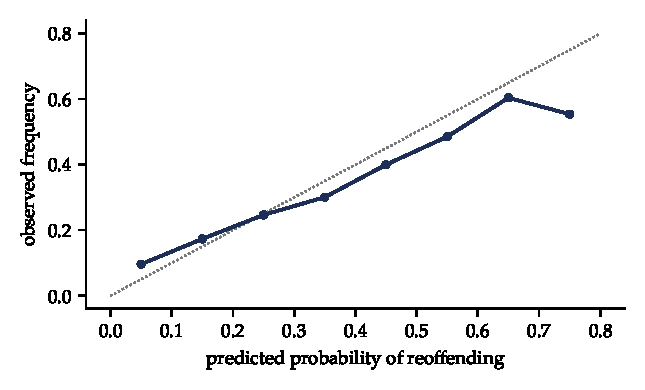
\includegraphics[width=\linewidth]{fig_calibration}
\caption{A calibration plot for a simulated risk tool. Predicted probabilities are grouped into bins, and the observed frequency of the outcome in each bin is plotted against the average prediction. A well calibrated tool lies on the diagonal.}
\label{fig:calibration}
\end{figure}

\subsection{The Bayesian view}

From a Bayesian standpoint, calibration is the natural requirement for a probability that will be used in a decision. A decision maker who maximises expected utility needs the probability that the event will occur, and only a calibrated score supplies it. Figure~\ref{fig:calibration} shows a calibration check. Error rate parity is a property of a decision rule, not of a probability. If society wants to move the error rates across groups, it can change the decision thresholds by group while keeping the probabilities calibrated, which is a choice about utilities. One threshold per group can in general equalise only one error rate, not both, and equalising both would need randomisation. Group-specific thresholds also raise legal problems: a threshold that depends on race is an explicit racial classification, which in the United States invites equal protection scrutiny and in England and Wales claims of direct discrimination under the Equality Act 2010. Separating the probability from the decision, as Lindley would, clarifies what the fairness debate is about: whether the utilities used in a decision should differ across groups, a question of values as much as of statistics, and one the law constrains.

There is a further point. A calibrated score may be calibrated on biased data. If arrests, not offences, are the outcome, and if policing is more intensive in some neighbourhoods, then the score predicts arrests, and its calibration reproduces the bias of policing. The Bayesian remedy is to model the measurement process, the relation between offences and arrests, explicitly, rather than to treat the observed outcome as the truth. This is the same lesson as the selective labels problem: a model is only as good as its account of how its data were generated.

\section{Lindley's answer}

We can now state what we take to be Lindley's answer to his own challenge, translated into requirements for machines in courts.

\begin{keybox}
Requirements for a Bayesian machine in court.
\begin{enumerate}[label=\arabic*.]
\item Probabilities, not verdicts. The machine reports calibrated probabilities with stated uncertainty, not bare conclusions.
\item Explicit utilities. The losses used in any decision rule are stated, set by legislatures or courts, and open to challenge.
\item Separation. The probability model and the decision rule are separate, so that each can be examined and changed independently.
\item Calibration checks. The machine's probabilities are tested for calibration, overall and within groups, on data from the population where it is used.
\item A model of the data. The machine's account of how its training data were generated, including selection and measurement, is documented.
\item Verifiable computation. The arithmetic from inputs to outputs can be checked by the parties.
\item Contestability. A party can challenge any input, and the effect of the challenge on the output is shown.
\item Human responsibility. A person, identified and accountable, adopts the decision and gives reasons.
\end{enumerate}
\end{keybox}

These requirements are demanding, and few current systems meet them. The proprietary risk tool in \emph{Loomis} met almost none: its model was secret, its utilities implicit, and its fairness disputed. ProPublica challenged its error rates across race, while its developer \citep{dieterich2016} and Flores, Bechtel and Lowenkamp argued that it was calibrated and satisfied predictive parity \citep{flores2016}. A tool built to these requirements would be more transparent than most human decision making, which is the point Lindley would have made. A judge does not state her probabilities or utilities, and her calibration is rarely checked. The question is not whether machines are perfect but whether a machine held to these standards, and overseen by a judge, would make better decisions than a judge alone. For many routine decisions, we think the answer is yes. For the hardest decisions, those that turn on contested facts, open texture and values, the machine can inform but should not decide.

Lindley's own view, as we understand it, was characteristically blunt: coherence is coherence, whoever achieves it. A court that reasons incoherently does injustice whether it is staffed by people or by machines. The opportunity that AI offers is to make the structure of legal reasoning explicit, so that incoherence can be seen and corrected. The danger is that it will be used to hide the structure further, behind proprietary models and fluent text. Which of these happens depends on choices that lawyers, judges and legislators are making now.

\section*{Notes and Questions}
\addcontentsline{toc}{section}{Notes and Questions}
\begin{enumerate}[label=\arabic*.]
\item Read \emph{State v Loomis}. Which of the eight requirements did the risk tool satisfy? What would the court have had to require to satisfy the rest?
\item Show that if two groups have different base rates and a yes or no classification has the same positive predictive value and the same false negative rate in each group, then its false positive rates differ unless its positive predictive value is zero or one. (Hint: write the false positive rate in terms of the base rate, the positive predictive value and the false negative rate.)
\item A video purports to show the defendant at the scene. An expert estimates that, if the defendant was not at the scene, the probability that a fabricated video of this quality would exist is one in a thousand. What is the maximum likelihood ratio of the video? How should the court proceed if authenticity is disputed?
\item Kleinberg and colleagues faced the selective labels problem. Explain it, and explain how quasi random assignment of judges helps.
\item Using the Priest and Klein model, predict how better outcome prediction would change the composition of cases reaching trial and the plaintiff win rate.
\item Draft a practice direction for the use of language models by judges in your jurisdiction. Which of the ten channels in this chapter does it address?
\item Should France's ban on analytics about individual judges be adopted elsewhere? Argue both sides in terms of noise, value of information and judicial independence.
\end{enumerate}

\section*{Further reading}
Kleinberg and colleagues on bail \citep{kleinberg2018}; Chouldechova \citep{chouldechova2017} and Kleinberg, Mullainathan and Raghavan \citep{kleinberg2017} on fairness; Susskind on online courts \citep{susskind2019}; Kahneman, Sibony and Sunstein on noise \citep{kahneman2021}.

\chapter{Verifying AI, Explaining AI and the Ethics of Legal Machines}
\label{ch:xai}

\section{Three questions}

Chapter~\ref{ch:lean} asked how formal verification could check the logical and arithmetical steps of legal decisions. Chapter~\ref{ch:lindleyai} described how artificial intelligence is changing court decisions and set out requirements for a Bayesian machine in court. This chapter takes up three questions that bridge the two. How can the outputs of AI systems, especially language models, be verified before courts and lawyers rely on them? How can the reasoning of an AI system be explained to the people its decisions affect? And what ethical principles should govern the use of AI in legal decision making? Each question has a Bayesian answer, and each answer connects to an emerging body of law.

\section{Verification with AI}

\subsection{The verification problem}

A language model asked a legal question produces fluent text. Some of it is correct, some is subtly wrong, and some, as \emph{Mata v Avianca} showed \citep{mata2023}, is invented. The model's fluency is not evidence of its accuracy; the likelihood ratio of a fluent answer, for the proposition that it is correct, may be little more than one. Verification is the process of raising that likelihood ratio by checking the output against sources and constraints that the model did not control.\index{verification!of AI outputs}

We distinguish four layers of verification, from the most mechanical to the most judgmental.

\paragraph{Existence and citation} Every authority cited must exist and say what the output claims. This can be checked automatically against databases of judgments and statutes. A citation that does not resolve to a real document is a certain error. A citation that resolves but does not support the proposition requires reading. Tools that retrieve the cited passage and display it next to the claim make the second check fast.

\paragraph{Logical structure} The output's argument must have the form required by the law: the elements of a claim addressed, the exceptions considered, the conclusion following from the findings. This is the layer that formal verification addresses. A language model that proposes an argument and a checker that verifies its structure against an encoding of the rules form a loop now increasingly used in mathematics, where models propose proof steps and Lean checks them.

\paragraph{Arithmetic and probability} Any computation in the output, a damages figure, a limitation period, a likelihood ratio, must be recomputed by a trusted tool. Language models are unreliable at arithmetic, and their errors can be large. The interval certificates of Chapter~\ref{ch:lean} apply.

\paragraph{Judgment} Finally, the output's characterisation of facts, its interpretation of open textured terms and its weighing of considerations must be assessed by a person. Verification cannot replace this layer, but by removing errors in the first three it lets the person concentrate on it.

\subsection{Retrieval and grounding}

The most common technical response to invented authority is retrieval augmented generation: the model is given relevant documents retrieved from a trusted database and instructed to answer from them, citing passages. Grounding reduces but does not eliminate error, because the model may misread or misrepresent the retrieved text, and the retrieval may miss the most relevant authority. A Bayesian evaluation of such systems measures their error rates on realistic tasks: the probability that a cited passage does not support the claim, the probability that a controlling authority is missed. These rates determine the likelihood ratio of the system's output and therefore how much a lawyer may rely on it without independent checking.

\subsection{Calibration and conformal guarantees}

A system that reports its confidence is more useful than one that does not, provided its confidence is calibrated: among answers given with ninety per cent confidence, about ninety per cent should be correct. Language models are often poorly calibrated, expressing high confidence in wrong answers. Calibration can be measured and improved, and it should be reported for any system used in legal work, as Chapter~\ref{ch:lindleyai} required for risk tools.\index{calibration}

Conformal prediction offers a stronger guarantee under mild assumptions. Given a set of past cases with known answers, a conformal procedure constructs, for a new case, a set of possible answers that contains the correct one with a specified probability, such as ninety five per cent, whatever the underlying model \citep{angelopoulos2023}. The guarantee holds on average over cases, not for each case separately. For legal classification tasks, such as predicting which of several issues will be decisive or which category a document belongs to, conformal sets give the user a guarantee of coverage: if the set contains several answers, the system is uncertain and the user knows to look harder. The guarantee depends on the new case being exchangeable with the calibration cases, an assumption that fails when the law changes or the case is unusual, so conformal methods must be recalibrated as the law develops.\index{conformal prediction}

\subsection{Adversarial checking}

The adversarial system of the common law is itself a verification procedure: each side checks the other's claims. AI can be used the same way. A second model, or the same model prompted differently, can be asked to find errors in an output, to argue the opposite position, or to identify authorities the first output missed. Agreement between independent checks raises confidence; disagreement flags a point for human attention. The Bayesian caution is that two models trained on similar data are not independent, so their agreement is weaker evidence than agreement between independent human reviewers. Independence must be engineered, by using different models, different sources or different prompts, and its degree estimated.

\subsection{Audit trails}

Verification after the fact requires a record. A system used in legal decision making should keep a log of its inputs, the documents it retrieved, its outputs and the checks performed, so that a party challenging a decision can see how it was produced. The European Union's AI Act requires high risk systems, including those intended to assist judicial authorities, to keep logs enabling traceability \citep{euaiact2024}. Logs also make it possible to measure error rates in practice, closing the loop between deployment and evaluation.

\section{Explainable AI}

\subsection{What an explanation is for}

A person affected by a decision is entitled, in most legal systems, to reasons. Reasons serve several purposes: they let the person understand why the decision was made, assess whether it was correct, and challenge it if not; they discipline the decision maker, who must articulate a justification; and they let others learn from the decision, which in the common law is how precedent is made. An AI system that produces decisions without reasons, or with reasons that do not reflect how the decision was actually reached, defeats all of these purposes.\index{explainable AI}

Explainable AI is the field that seeks to make the outputs of machine learning models understandable. It is useful to distinguish explanations of a model in general, which describe how it uses its inputs across all cases, from explanations of an individual decision, which describe why this case received this output. Legal reasons are mostly of the second kind.

\subsection{Feature attribution}

The most widely used methods attribute an individual prediction to the input features. LIME fits a simple local model to perturbed samples around the case and reports its coefficients \citep{ribeiro2016}. SHAP assigns each feature a contribution based on Shapley values from cooperative game theory, so that the contributions sum to the difference between the prediction and a baseline \citep{lundberg2017}. These methods are general and widely implemented. They also have limitations: attributions can change with the choice of baseline, can be unstable for correlated features, and describe the model's behaviour, not the world. An attribution that says a defendant's postcode contributed heavily to a high risk score explains the model, and may reveal that the model is using a proxy for race, but it does not justify the score.

\subsection{Counterfactual explanations}

Wachter, Mittelstadt and Russell proposed counterfactual explanations: statements of the smallest change to the input that would have changed the decision, such as (our illustration) your loan would have been approved if your income had been five thousand pounds higher \citep{wachter2018}. Counterfactual explanations have attractive legal properties. They tell the person what would have made a difference, which is what they need to contest or act on the decision, and they do not require disclosing the model. They correspond closely to the but for reasoning of causation discussed in Chapter~\ref{ch:tort}. Their weakness is that many counterfactuals may exist, and the one reported may not be the most useful or the most realistic.\index{counterfactual explanations}

\subsection{Weight of evidence as explanation}

A Bayesian model offers a native form of explanation that predates the field of explainable AI by decades. When a decision depends on a posterior, and the posterior is built from a prior and likelihood ratios for items of evidence, the explanation is the ledger of weights. Good's weight of evidence, introduced in Chapter~\ref{ch:odds}, decomposes the log posterior odds into a prior term and a sum of contributions, one for each item:
\begin{equation}
\label{eq:woe-ledger}
10\log_{10}\odds(H\given E_1,\ldots,E_k) = 10\log_{10}\odds(H) + \sum_{i=1}^k W(H : E_i \given E_1,\ldots,E_{i-1}),
\end{equation}
where $W(H : E_i \given E_1,\ldots,E_{i-1})$ is ten times the base ten logarithm of the likelihood ratio for $E_i$ given the earlier items, in decibans as in Chapter~\ref{ch:odds}. For conditionally independent items the conditioning drops away and the weights are those of the items taken one at a time. Such an explanation is faithful by construction: it is the computation the model performed, not an approximation to it. It is also in a form lawyers can engage with: each weight is a claim about how much more probable an item is under one hypothesis than the other, which can be contested with evidence. Good and Card studied the expected weight of evidence as a quasi-utility in the analysis of diagnostic error \citep{goodcard1971}, and the case made here for weights as the language of explanation applies with equal force in law.\index{weight of evidence!as explanation}

This is a strong reason to prefer, for high stakes legal decisions, models whose structure is Bayesian and interpretable over black box models explained after the fact. Cynthia Rudin has argued that for high stakes decisions one should use inherently interpretable models rather than attempt to explain black boxes \citep{rudin2019}, and work on certifiably optimal rule lists reports that for recidivism prediction an interpretable model can match a complex one in accuracy \citep{angelino2018}. The Bayesian networks of Chapter~\ref{ch:graphs}, the hierarchical models of Chapters~\ref{ch:llsv} and~\ref{ch:africa}, and the weight of evidence ledgers of Chapter~\ref{ch:stories} are interpretable in this sense.

\subsection{The legal right to an explanation}

Article 22 of the European Union's General Data Protection Regulation gives individuals a right not to be subject to decisions based solely on automated processing that produce legal or similarly significant effects, subject to exceptions with safeguards. Whether the regulation also confers a right to an explanation of such decisions was debated for years. The AI Act now provides, in Article 86, that a person subject to a decision taken by a deployer on the basis of the output of a high risk AI system listed in Annex III (other than the systems in point 2 of that Annex), which produces legal effects or similarly significantly affects the person in a way they consider adverse to their health, safety or fundamental rights, has the right to obtain clear and meaningful explanations of the role of the AI system in the decision procedure and the main elements of the decision taken, unless Union or national law provides otherwise \citep{euaiact2024}. Article 13 requires high risk systems to be designed so that deployers can interpret their output, and Article 14 requires effective human oversight.\index{right to explanation}

These provisions do not specify a method of explanation. A Bayesian reading of the requirement of clear and meaningful explanations of the main elements of the decision suggests that a weight of evidence ledger, or a counterfactual statement of what would have changed the outcome, satisfies it, while a list of feature attributions from a post hoc approximation may not, if it does not faithfully reflect the decision. Courts will have to decide.

\section{Ethics of legal AI}

\subsection{Principles}

Many bodies have issued principles for the ethical use of AI. For courts specifically, the European Commission for the Efficiency of Justice of the Council of Europe adopted in 2018 a European Ethical Charter on the use of artificial intelligence in judicial systems, setting out five principles: respect for fundamental rights; non discrimination; quality and security, including the use of certified sources and secure environments; transparency, impartiality and fairness, including making methods accessible and understandable; and user control, meaning that users must be informed actors in control of their choices \citep{cepej2018}. UNESCO's 2021 Recommendation on the Ethics of Artificial Intelligence and the Council of Europe's 2024 Framework Convention on Artificial Intelligence and Human Rights, Democracy and the Rule of Law state broader principles applicable to all public uses.\index{ethics of AI}\index{CEPEJ ethical charter}

These principles converge on a few themes: fairness, transparency, accountability, human oversight, privacy and respect for rights. They are stated at a high level of generality, and their application to particular systems requires judgment. A Bayesian framework helps by translating several of them into measurable requirements.

\subsection{Fairness as calibration and as utility}

Chapter~\ref{ch:lindleyai} explained the impossibility results. Kleinberg, Mullainathan and Raghavan showed that a risk score cannot simultaneously be calibrated within groups and balanced for the positive class and for the negative class (equal mean score among actual reoffenders, and among non-reoffenders, across groups) unless prediction is perfect or base rates are equal \citep{kleinberg2017}. Chouldechova showed that a yes or no classification with equal positive predictive value across groups cannot also have equal false positive and equal false negative rates when prevalences differ, unless its positive predictive value is zero or one \citep{chouldechova2017}. The ethical question is which property to prioritise, and the Bayesian answer is to separate the two. Probabilities should be calibrated, because only calibrated probabilities support coherent decisions. Error rates are properties of decisions, determined by thresholds, which are determined by utilities. If society judges that the costs of errors differ across groups, for instance because historical disadvantage makes detention more harmful for some, it can set different thresholds, and must say so openly; as Chapter~\ref{ch:lindleyai} noted, one threshold per group cannot in general equalise both error rates, and a threshold that depends on race invites equal protection scrutiny in the United States and claims of disparate treatment elsewhere. Fairness then becomes a matter of explicit utilities, debated and decided by legitimate institutions, not of hidden adjustments to probabilities.

\subsection{Accountability}

When an AI system contributes to a wrong decision, who is responsible? The deployer, the developer, the judge who relied on it? Legal accountability requires that some person be answerable. The requirement in Chapter~\ref{ch:lindleyai} that a human adopt the decision and give reasons is partly an accountability requirement. It must not become a formality, in which a judge rubber stamps machine output. Automation bias, the tendency to defer to automated recommendations, is well documented \citep{parasuraman2010}, and, in our reading, its strength grows as systems become more accurate in ordinary cases, since people learn to trust them. An ethical deployment must therefore include measures that keep human judgment active: requiring the judge to record her own assessment before seeing the machine's, periodically auditing cases where the judge followed the machine, and training judges in the system's failure modes.\index{automation bias}

\subsection{Dignity and the right to a human judge}

Some argue that there is a right to be judged by a human being, independent of accuracy, grounded in human dignity: a person facing a court is entitled to be heard by someone who can understand his situation as a fellow person. Lindley's challenge confronts this argument directly. If a machine decides more accurately and more consistently, is the insistence on a human judge a preference for ritual over justice? There are several answers. The right to be heard by a person may be part of what makes a decision legitimate in the eyes of those subject to it, and legitimacy has consequences for compliance and for trust in law. A human judge can recognise circumstances outside the model, the novel fact that no training data anticipated. And the values that determine utilities, as Lindley said, must come from people. A reasonable synthesis is that machines may compute and recommend, while persons must decide, hear and take responsibility, at least where liberty, family or fundamental rights are at stake.

\subsection{Privacy and data}

Legal AI is trained on legal data: judgments, filings, records of proceedings. These contain personal information, often sensitive. Using them for training raises questions of data protection, confidentiality and consent. The French restriction on analytics about judges, discussed in Chapter~\ref{ch:commoncivil}, is one response; anonymisation of published judgments is another. The Bayesian perspective adds a point about information: the value of legal data for learning is high, and restrictions on its use impose a cost in less accurate systems. The trade off between privacy and accuracy should be made explicitly, with techniques such as differential privacy used where they allow useful learning with formal privacy guarantees.

\subsection{Ethics as expected utility}

Finally, it is worth saying what a Bayesian ethics of legal AI is not. It is not the claim that every ethical question reduces to a calculation. It is the claim that once a society has stated its values, as utilities, and its knowledge, as probabilities, coherent action follows, and that departures from coherence are errors. Many ethical failures of AI systems, in the law and elsewhere, are failures of this kind: systems whose implied utilities were never stated or examined, whose probabilities were never calibrated, whose decisions could not be explained because no one knew what they were maximising. Making the structure explicit is itself an ethical act, because it subjects the system to scrutiny. That, again, was Lindley's point.

\section*{Notes and Questions}
\addcontentsline{toc}{section}{Notes and Questions}
\begin{enumerate}[label=\arabic*.]
\item Design a verification protocol for a law firm's use of a language model to draft research memoranda. Which of the four layers can be automated, and what error rates would you require before relying on each?
\item Explain the difference between a feature attribution and a counterfactual explanation for a bail decision. Which better serves a defendant wishing to challenge the decision?
\item Write the weight of evidence ledger for the Adams case of Chapter~\ref{ch:odds}. Is it a sufficient explanation of the posterior?
\item Article 86 of the AI Act requires clear and meaningful explanations of the main elements of a decision. Would a SHAP plot satisfy it? A weight of evidence ledger?
\item Assess a risk assessment tool used in your jurisdiction against the five principles of the CEPEJ charter.
\item Is there a right to be judged by a human being? Argue both sides, and say how your answer depends on the kind of decision.
\end{enumerate}

\section*{Further reading}
Rudin on interpretable models \citep{rudin2019}; Wachter, Mittelstadt and Russell on counterfactual explanations \citep{wachter2018}; Lundberg and Lee on SHAP \citep{lundberg2017}; Angelopoulos and Bates on conformal prediction \citep{angelopoulos2023}; the CEPEJ charter \citep{cepej2018}.

\chapter{Intuition, Miracles and the Limits of Human Judgment}
\label{ch:hume}

\begin{quote}\itshape
A wise man, therefore, proportions his belief to the evidence.
\par\hfill\normalfont David Hume, \emph{Of Miracles}, 1748
\end{quote}

\section{Odds, not opinions}

Courts are full of opinions. Witnesses believe they saw the defendant; experts are of the opinion that the injury was not accidental; counsel submit that a story is implausible; judges find that a witness was credible. Opinions are the raw material of adjudication, and the law could not function without them. But an opinion is not a probability, and a fact finder who adopts the most confident opinion, or the most eloquent, is not reasoning. The task is to weigh: to ask how probable the evidence would be if each account were true, and to combine that with how probable each account was to begin with. This chapter argues that this weighing is exactly what unaided human intuition does badly, that two and a half centuries of thought from Hume to Lindley explain why, and that the empirical evidence on human and mechanical judgment supports Lindley's view that coherent procedures, including machines, will often do better than people left to themselves.

\section{Hume on miracles}

\subsection{The argument}

In the tenth section of his \emph{Enquiry Concerning Human Understanding}, published in 1748, David Hume considered what testimony could establish the occurrence of a miracle. His answer has become one of the most famous arguments in philosophy. A miracle is a violation of the laws of nature, and those laws are established by uniform experience. Testimony, too, derives its authority from experience: we trust witnesses because we have found that people usually report truly. When testimony asserts a miracle, the two kinds of experience conflict, and we must weigh them. Hume's conclusion was a maxim:
\begin{quote}
No testimony is sufficient to establish a miracle, unless the testimony be of such a kind, that its falsehood would be more miraculous, than the fact, which it endeavours to establish.
\end{quote}
And he summarised the method in a phrase: a wise man proportions his belief to the evidence.\index{Hume, David}\index{miracles}

\subsection{Hume as a Bayesian}

Hume did not use Bayes' theorem, which was published by Richard Price only in 1763, partly, it has been suggested, as a reply to Hume. But his maxim is a statement about posterior odds. Let $M$ be the proposition that the miracle occurred and $T$ the testimony that it did. Then
\begin{equation}
\frac{\Prob(M\given T)}{\Prob(\bar M\given T)} = \frac{\Prob(T\given M)}{\Prob(T\given \bar M)}\cdot\frac{\Prob(M)}{\Prob(\bar M)} .
\end{equation}
The prior odds of a miracle are tiny, since it violates laws established by uniform experience. The testimony establishes the miracle, in the sense of making it more probable than not, only if the likelihood ratio exceeds the reciprocal of the prior odds: only if $\Prob(T\given\bar M)$, the probability that such testimony would be given though the miracle did not occur, is smaller than $\Prob(T\given M)\,\Prob(M)/\Prob(\bar M)$, which for a tiny prior is essentially $\Prob(M)$ times $\Prob(T\given M)$. Equivalently, $\Prob(T\text{ and }\bar M)<\Prob(T\text{ and }M)$: the falsehood of the testimony must be less probable, more miraculous, than the miracle itself. Hume's maxim is the condition that the posterior odds exceed one.\index{Hume's maxim}

John Earman criticised Hume's argument as an abject failure, on the central ground that Hume did not see how independent witnesses can combine to overcome a small prior \citep{earman2000}. If each of many independent witnesses has a likelihood ratio of ten, then twenty of them supply a combined likelihood ratio of $10^{20}$, enough to overcome even small priors. Whether Hume missed this is debated. For our purposes the important point is that the Bayesian framework both vindicates Hume's maxim and shows its limits: it is correct as a condition on a single body of testimony, and it correctly implies that sufficiently many independent witnesses could establish an extraordinary event. The key word is independent. Witnesses who share a source, a motive or an enthusiasm are not independent, and their combined weight is far less than the product.

\subsection{Hume in court}

Hume's argument applies to law with little change. Courts are regularly asked to find that extraordinary things happened: that a respectable professional committed a grave fraud, that a parent harmed a child, that a nurse murdered patients, that a company knowingly concealed a lethal defect. Each allegation has a low prior, because such conduct is rare. Each is supported by testimony and other evidence whose falsehood or misleadingness has some probability. Hume's maxim tells the fact finder what to ask: is the evidence of such a kind that its being misleading would be more improbable than the allegation itself?

This is exactly the reasoning of Lord Nicholls in \emph{Re H} \citep{reh1996}, discussed in Chapter~\ref{ch:standards}: the more serious the allegation, the less likely it is that the event occurred, and hence the stronger the evidence needed. Lord Nicholls was applying Hume's maxim to the civil standard of proof. Lady Hale's correction in \emph{Re B} (2008) \citep{reb2008}, that seriousness does not always imply improbability, is also Humean: the prior depends on the circumstances, and, as Lord Hoffmann observed in the same case, where a child was injured by one of only two people, one of them certainly did, so seriousness says nothing about which.

The medical murder cases of Chapter~\ref{ch:clusters} are the most direct application. The prior that a particular nurse is a serial killer is small. The evidence typically includes a statistical association and expert medical opinion. Hume would ask: what is the probability that such an association and such opinions would arise if the nurse were innocent, given how the cases were identified and how the experts were instructed? If that probability is not much smaller than the prior probability of murder, the evidence does not establish guilt, however confident the experts.

\section{Human intuition}

\subsection{Heuristics and biases}

Kahneman and Tversky's research program showed that people reasoning about uncertainty rely on heuristics, mental shortcuts that are often useful and sometimes systematically wrong \citep{tversky1974}. The representativeness heuristic leads people to judge probability by resemblance, neglecting base rates, as in the cab problem of Chapter~\ref{ch:odds}. The availability heuristic leads them to judge frequency by how easily examples come to mind, so that vivid evidence is overweighted. Anchoring leads them to adjust insufficiently from an initial value, even an irrelevant one. The studies below document anchoring, framing, hindsight bias and related effects in legal decision makers.\index{heuristics and biases}

\subsection{Judges are human}

Studies of experienced judges confirm that expertise does not immunise against these effects. Englich, Mussweiler and Strack asked experienced German legal professionals to sentence a hypothetical shoplifting case after rolling dice that had been loaded to produce a high or a low number, presented as the prosecutor's demand; participants who rolled higher numbers gave longer sentences \citep{englich2006}. Guthrie, Rachlinski and Wistrich found that American federal magistrate judges were susceptible to anchoring, hindsight bias and egocentric bias, though they did better than lay people on framing and representativeness \citep{guthrie2001}. Studies of asylum adjudication in the United States found large differences in grant rates between judges in the same court hearing similar cases, a phenomenon its authors called refugee roulette \citep{ramji2007}. A widely cited study of Israeli parole boards reported that favourable decisions fell over the course of each session and recovered after food breaks \citep{danziger2011}; the finding has been disputed, on the ground that the order of cases was not random, and is best treated as illustrating the questions rather than settling them. Kahneman, Sibony and Sunstein collected evidence that unwanted variability, which they call noise, is pervasive in professional judgment, including sentencing \citep{kahneman2021}.\index{anchoring}\index{noise}

\subsection{When intuition works}

Intuition is not always unreliable. Kahneman and Klein, who had long disagreed about expert intuition, agreed in a joint paper on the conditions under which it can be trusted: the environment must be regular enough to be predictable, and the expert must have had extensive practice with rapid and accurate feedback \citep{kahneman2009}. Chess masters, firefighters and anaesthetists meet these conditions. Judges deciding facts usually do not. A judge who finds a witness credible rarely learns whether the witness was in fact telling the truth. Appellate review is built to correct legal errors and defers heavily to findings of fact, and wrongful convictions are discovered years later, if ever. In an environment without feedback, intuition does not calibrate, and confidence becomes unrelated to accuracy. This is the core of the case for structured, explicit reasoning in fact finding.

\section{Clinical versus statistical judgment}

\subsection{Meehl's disturbing little book}

In 1954 the psychologist Paul Meehl published \emph{Clinical versus Statistical Prediction}, comparing the accuracy of predictions made by trained clinicians using their judgment with predictions made by simple statistical formulas using the same information \citep{meehl1954}. In study after study the formulas did at least as well as the clinicians, and often better. Meehl called it his disturbing little book. Half a century later, Grove and colleagues conducted a meta analysis of over a hundred studies comparing clinical and mechanical prediction across medicine, psychology, education and criminal justice; mechanical prediction was about as accurate or more accurate in the great majority, and clinical prediction was substantially better in only a small minority \citep{grove2000}.\index{Meehl, Paul}\index{clinical versus statistical prediction}

Robyn Dawes added a striking result: even improper linear models, with weights chosen arbitrarily, such as equal weights on standardised predictors, outperform clinical judgment in many settings, because the main advantage of the formula is its consistency \citep{dawes1979}. A human expert knows which variables matter but applies them inconsistently, distracted by irrelevant detail, swayed by vivid cases and influenced by mood. The formula applies the same weights to every case.

\subsection{Bail and sentencing}

The Kleinberg study of bail decisions in New York, discussed in Chapter~\ref{ch:lindleyai}, is Meehl's comparison applied to a legal decision with careful attention to the selective labels problem \citep{kleinberg2018}. The machine learning rule, using only information available to the judges, could have reduced crime substantially at the same detention rate. The judges' errors appeared to reflect responding to noise, including unobservable features of the case, as if it were signal.

\section{Lindley's point}

Lindley's point is the ground of the challenge set out in Chapter~\ref{ch:why}. He drew the conclusion that the evidence of Meehl, Kahneman and Tversky invites. People are not coherent; they do not reason according to the rules of probability, nor act to maximise expected utility. In \emph{Understanding Uncertainty} he acknowledged the descriptive evidence that people are not rational in the economist's sense, and responded not by revising the normative theory but by arguing that everyone should be taught probability, utility and the maximisation of expected utility, and should act accordingly \citep{lindley2006}. His view of the law, as we understand it, followed. A court that decided by the rules of coherent reasoning would do better than one that relied on intuition, and since machines can be built to follow those rules exactly, while people cannot, a properly designed machine would in many respects be a better judge of facts than a person.\index{Lindley, Dennis}

We should be precise about what this point claims. It does not claim that machines understand the world better than people, or that they should decide what society values. It claims that, given the same information and the same utilities, a procedure that combines them coherently will on average make better decisions (higher expected utility under the stated probabilities and utilities) than a procedure that combines them incoherently, and that unaided human judgment is demonstrably incoherent in predictable ways. The evidence from Meehl onwards supports this claim for prediction tasks with clear outcomes. Legal fact finding is harder, because outcomes are rarely observed, but the biases that make human prediction inferior are the same ones that operate in fact finding.

The practical upshot is not to replace judges with machines but to change what judges do. Judges should state their probabilities and their reasons in a form that can be checked; they should use structured tools, such as likelihood ratio ledgers and decision thresholds, where the stakes justify the effort; and they should use machines to compute, check and flag, while reserving to themselves the tasks that require understanding and values. A judge who weighs odds rather than opinions, aided by tools that keep the arithmetic straight, combines the strengths of each.

\section{Weighing testimony: a procedure}

Hume's maxim and Lindley's point suggest a procedure that any fact finder can follow, with or without numbers.
\begin{enumerate}[label=\arabic*.]
\item State the propositions in issue and their alternatives, including alternatives no party has advanced.
\item For each, ask how probable it was before the specific evidence, considering base rates for conduct of this kind in circumstances of this kind.
\item For each item of evidence, ask how probable it would be under each proposition, including the probability that it would be misleading if the proposition were false: that a witness would be mistaken or lying, that a test would err, that an expert would be wrong.
\item Ask which items share sources, so that their likelihood ratios must not be multiplied as if independent.
\item Combine, and ask whether the result crosses the threshold the law sets, given the consequences of error.
\item Ask, with Hume, whether the falsehood of the evidence would be more improbable than the fact it is offered to prove. This is the balance-of-probabilities test; for a criminal standard it is necessary but not sufficient, and step 5 still governs.
\end{enumerate}
This procedure is the Bayesian method stated in words. It is what this book has recommended throughout. Its value lies less in any particular number than in the discipline of asking each question explicitly, so that intuition is checked at each step rather than trusted at the end.

\section*{Notes and Questions}
\addcontentsline{toc}{section}{Notes and Questions}
\begin{enumerate}[label=\arabic*.]
\item Express Hume's maxim as an inequality between $\Prob(M)$, $\Prob(T\given M)$ and $\Prob(T\given \bar M)$, keeping the factor $1/\Prob(\bar M)$. Show that it is exactly equivalent to the posterior odds exceeding one, and say when it reduces to $\Prob(T\given\bar M)<\Prob(M)\Prob(T\given M)$.
\item Ten independent witnesses each testify to an event with prior probability $10^{-6}$. Each witness has a likelihood ratio of five. What is the posterior probability? What if the witnesses all heard the story from one person?
\item Apply Hume's maxim to an allegation of fraud against a long serving and well regarded professional. What kind of evidence would satisfy it?
\item Design an experiment, in the manner of Englich, Mussweiler and Strack, to test whether a likelihood ratio direction reduces anchoring in civil damages awards.
\item Kahneman and Klein identify conditions under which intuition is reliable. Which legal tasks, if any, meet them?
\item Is Lindley's point an argument for machine judges? State the strongest version of the argument and the strongest objection.
\end{enumerate}

\section*{Further reading}
Hume's \emph{Of Miracles}, section ten of the \emph{Enquiry}; Earman's \emph{Hume's Abject Failure} \citep{earman2000}; Meehl \citep{meehl1954} and Grove and colleagues \citep{grove2000}; Kahneman, Sibony and Sunstein on noise \citep{kahneman2021}; Lindley's \emph{Understanding Uncertainty} \citep{lindley2006}.

\chapter{A Bayesian Program for the Law}
\label{ch:program}

\section{What we have argued}

This book has made a single argument in many settings. Legal decisions are decisions under uncertainty. The coherent way to make such decisions is to measure uncertainty by probability, to update probabilities by Bayes' rule, to measure consequences by utility, and to choose the action that maximises expected utility. The law already does much of this implicitly. Standards of proof are posterior thresholds set by ratios of losses. Relevance is a likelihood ratio different from one. Negligence is a failure to minimise expected cost given reasonable beliefs. Misrepresentation is a gap between conveyed and warranted belief. Stories are generative models compared by their marginal likelihoods. Solvency is a probability of default at a past date. Skill is a share of variance. Procedure is a strategy for acquiring information. Courts are queues. Deterrence is expected sanction. And machines are useful in courts exactly to the extent that they make these structures explicit and checkable.

Where the law departs from coherent reasoning, it pays a price. Statistical fallacies, the prosecutor's fallacy among them, helped convict Sally Clark. The Dershowitz fallacy misdirected public argument in Simpson. The all or nothing rule in \emph{Gregg v Scott} denies compensation for real losses and gives doctors the wrong incentives. Hindsight bias distorts fraudulent transfer litigation. The refusal to quantify the effect of contamination left the Kercher courts reweighing the same two items for more than seven years. Delay in India punishes the presumed innocent. Each departure has an identifiable cost, and each can be reduced.

\section{Ten proposals}

We close with ten proposals, each of which follows from earlier chapters and could be adopted without changing the fundamental structure of any legal system.

\paragraph{1. Report likelihood ratios with ranges} Every forensic report presented in court should state a likelihood ratio, or range of likelihood ratios, for the propositions in issue, with the inputs and their sources, including laboratory error rates and transfer probabilities. Verbal scales may accompany the numbers but should not replace them. (Chapters~\ref{ch:odds},~\ref{ch:classic} and~\ref{ch:bf}.)

\paragraph{2. Direct juries on conditioning} Judicial directions should explain the difference between the probability of the evidence given innocence and the probability of innocence given the evidence, and should warn against conditioning on the wrong event. Model directions could use the island problem and the Simpson argument as illustrations. (Chapters~\ref{ch:odds},~\ref{ch:classic} and~\ref{ch:fallacies}.)

\paragraph{3. Separate activity from source} Courts should require experts to address separately whose trace was found and how it got there, and should recognise that the second question, which turns on transfer and contamination, often determines the case. (Chapters~\ref{ch:bf} and~\ref{ch:stories}.)

\paragraph{4. Proportionate remedies where causation is probabilistic} English law should extend proportionate recovery for lost chances to clinical negligence, as French law and the English law of lost commercial chances already do, and as the Insurance Act 2015 does for breaches of the duty of fair presentation that are neither deliberate nor reckless. (Chapters~\ref{ch:tort},~\ref{ch:misrep} and~\ref{ch:commoncivil}.)

\paragraph{5. Judge representations by their implied distributions} Representations about the safety of investments should be assessed by what they imply about the probability of large losses, not only by expected values, and chains of reliance should be analysed for their weakest link. (Chapter~\ref{ch:greensill}.)

\paragraph{6. Combine market and expert evidence of solvency} In fraudulent transfer and wrongful trading cases, courts should combine contemporaneous market evidence with expert analysis, weighting each by its reliability and correcting expert evidence for hindsight. (Chapter~\ref{ch:bankruptcy}.)

\paragraph{7. Use single joint experts and require distributions} Courts should make greater use of single joint or court appointed experts, and should require all experts to report distributions and sensitivity analyses rather than point estimates. (Chapters~\ref{ch:fienberg} and~\ref{ch:kadane}.)

\paragraph{8. Triage by expected cost of delay} Overloaded court systems should schedule cases using estimates of the cost of delay and the time to decision, published and open to challenge, and should recognise in bail decisions that the cost of detention grows with expected delay. (Chapter~\ref{ch:india}.)

\paragraph{9. Publish law as code where it is computation} Statutory rules that compute entitlements and liabilities should be published in a formal language alongside the text, and administrative software should be tested against them. Computations presented in court should be machine checkable. (Chapter~\ref{ch:lean}.)

\paragraph{10. Hold machines to Bayesian standards} Machine tools used in courts should report calibrated probabilities, separate probability from decision, state their utilities, document their data, allow verification and contestation, and leave responsibility with an accountable person. (Chapter~\ref{ch:lindleyai}.)

\section{Objections revisited}

The objections to Bayesian legal reasoning set out in Chapter~\ref{ch:why} have been addressed throughout. The presumption of innocence is consistent with a prior of $1/N$. Probabilities of single events are degrees of belief, made coherent by the rules of probability and informed by frequencies. Numbers need not overwhelm soft evidence if the soft evidence is quantified too. To the objection that the law values reasons, not calculations, the reply is that a likelihood ratio is a reason. And the difficulty juries have with arithmetic is an argument for better presentation and better tools, not for abandoning coherence.

One objection deserves a final word. It is said that the law is a human practice, embedded in history, culture and politics, and that a mathematical theory of it misses what matters. We agree that the law is a human practice, and the chapters on comparative law, on Corsica and Sicily, on Cameroon and India, have tried to show how much of legal life lies outside any model. But a theory of rational belief and action is not a theory of everything. It is a discipline that applies wherever people must decide under uncertainty, which in law is almost everywhere. It does not tell us what to value; it tells us how to act consistently with what we value, given what we know. That is a modest claim, and it is enough to justify the program.

\section{The future}

Lindley expected that we would all be Bayesian by 2020. The law has been slower, for good reasons: its institutions are old, its practitioners are trained in words rather than numbers, and its legitimacy depends on public understanding. But the pressures are building. Forensic guidance in Europe has moved to likelihood ratios. Insurance law has adopted proportionate remedies. Courts weigh market evidence of solvency. Machine learning is entering every stage of litigation, and its outputs are probabilities. The question is no longer whether the law will use probability but whether it will use it well. Chapter~\ref{ch:future} returns to this question in closing.

We hope this book helps lawyers, statisticians and policy makers to use it well. The tools are old: Bayes' rule, expected utility, the weight of evidence. The settings are new: deepfakes, overloaded courts, global supply chains, machine judges. What remains constant is the obligation to reason coherently about what we do not know when the stakes are someone's liberty, property or life.

\section*{Notes and Questions}
\addcontentsline{toc}{section}{Notes and Questions}
\begin{enumerate}[label=\arabic*.]
\item Choose one of the ten proposals and draft a rule of court or statutory provision implementing it. What objections would you expect, and how would you answer them?
\item Which proposal would have changed the outcome of a case discussed in this book? Explain how.
\item Rank the ten proposals by their expected benefit relative to cost in your jurisdiction. What evidence would you need to make the ranking reliable?
\item Is there a domain of law in which Bayesian reasoning is inappropriate? Make the strongest case you can.
\end{enumerate}

\chapter{The Future and Promise of AI in Law}
\label{ch:future}

\section{A profession built on reasoning}

Law is a profession of reasoning under uncertainty. Lawyers predict what courts will do, judges decide what probably happened, legislators guess how people will respond to rules. For centuries these tasks were done by trained human judgment, aided by books, precedent and argument. Artificial intelligence is now able to perform parts of them: reading and summarising documents, finding authorities, drafting submissions, predicting outcomes, estimating risks. This final chapter looks forward. It asks what the profession will look like in ten to twenty years, what AI can promise, what it cannot, and why a lawyer trained in Bayesian reasoning will be better placed than one who is not to use it well.

\section{What will change}

\subsection{The cost of legal information will fall}

The most likely change is that legal information will become cheap. Questions that once required a junior lawyer's week, what the law is on a point, what the documents show, how similar cases came out, will be answered in minutes. The price of routine legal work will fall, and so will the price of access to legal advice for individuals and small businesses who cannot now afford it. The economic consequences are large: legal services are a substantial industry, and much of their cost is in tasks that could be automated; one industry study estimates that up to 74 percent of hourly billable tasks could be automated \citep{clio2024}.

\subsection{Prediction will become explicit}

Lawyers have always predicted, but implicitly: an experienced litigator's view that a claim has good prospects is a probability that is never stated. AI systems produce explicit probabilities. Clients, funders, insurers and courts will increasingly expect them. When probabilities are explicit, they can be checked against outcomes, and lawyers whose predictions are poorly calibrated will be found out. This is a large change in professional accountability, and it rewards exactly the skills this book teaches: understanding what a probability means, how it should be updated, and how to combine it with values to reach a decision.

\subsection{Disputes will be selected differently}

As Chapter~\ref{ch:becker} and Chapter~\ref{ch:lindleyai} explained, better prediction should lead to more settlements, since disputes go to trial when the parties disagree about the outcome. Courts will see a higher proportion of genuinely hard cases: novel questions of law, close questions of fact, and cases where one party has private information. The work of judges will become, on average, harder, and the cases that make precedent will be more concentrated at the frontier.

\subsection{Evidence will change}

AI changes evidence itself. Deepfakes pull the likelihood ratio of a recording toward one; machine analysis of communications produces new kinds of evidence with their own error rates; algorithmic decisions by employers, lenders and governments become the subject of litigation, with the algorithm's behaviour as the evidence. Courts will need experts who can explain the likelihood ratios of machine outputs, and lawyers who can cross examine them.

\subsection{Courts will triage}

Overloaded courts, from the Crown Court in England and Wales to the district courts of India, will use AI to schedule, triage and manage cases, as Chapter~\ref{ch:india} described for India and Chapter~\ref{ch:systemcosts} for the costs of delay. Online dispute resolution for small claims will expand. The routine end of the justice system will become faster and cheaper; the question is whether it will also become more accurate and fair, which depends on how the systems are built and governed.

\section{What AI can promise}

\subsection{Consistency}

Human judgment is noisy. Similar cases receive different outcomes depending on the judge and irrelevant anchors, as Chapter~\ref{ch:hume} discussed (the evidence on the time of day is disputed). A deterministic system gives the same output for the same input. Consistency is not justice, since a consistently wrong system is worse than an inconsistently right one, but in domains where the right answer is reasonably well understood, reducing noise is a large gain. Sentencing ranges, damages tariffs and benefit calculations are candidates.

\subsection{Coherence}

A machine can be built to reason coherently: to update by Bayes' rule, to combine evidence without double counting, to apply decision thresholds that match stated losses. Lindley's challenge, the subject of Chapter~\ref{ch:lindleyai}, was that such a machine would decide at least as well as an unaided person. The promise of AI in law is the promise of coherence at scale.

\subsection{Access}

In California, for example, the 2024 Justice Gap Study found that 85 percent of civil legal problems received no or inadequate legal help \citep{calbar2024}. AI can provide information, prepare documents and guide people through procedures at a cost close to zero. If it is accurate, this could be the largest expansion of access to justice\index{access to justice} in history. The Bayesian discipline of calibration and explanation, discussed in Chapter~\ref{ch:xai}, is what makes the difference between a guide people can trust and one that misleads them.

\subsection{Verification}

As Chapter~\ref{ch:lean} argued, formal verification can check the logical and arithmetical parts of legal reasoning. Combined with language models that propose arguments, it offers a model of legal work in which machines draft, verifiers check and people judge. In mathematics this model is already producing verified formal results to which both people and machines contribute. Law may be next.

\section{What AI cannot promise}

\subsection{Values}

AI cannot tell a society what to value. The ratio of losses that sets a standard of proof, the purposes of sentencing, the weight given to liberty against safety, are choices that belong to legitimate institutions. A machine can implement any choice coherently, and can show the consequences of each, but it cannot make the choice. Lindley said the utilities must come from people; that remains true.

\subsection{Facts not in the data}

A model trained on past cases knows only what the past contains. A new kind of fraud, a new technology, a new social arrangement, may lie outside its experience, and it may not know that it does not know. Human judges, with their general understanding of the world, may be better at recognising novelty. A well designed system flags cases that look unlike its training data; a poorly designed one confidently misclassifies them.

\subsection{Legitimacy}

People accept legal decisions partly because they are made by persons accountable to them, through processes they recognise as fair. Whether people will accept decisions made or shaped by machines is an empirical question, and the answer may depend on how the machines are used: as tools of transparent human judgment, or as opaque substitutes for it. The requirements set out in Chapter~\ref{ch:lindleyai}, among them probabilities rather than verdicts, explicit utilities, verifiable computation, contestability and human responsibility, are designed to preserve legitimacy.

\section{The lawyer of the future}

What should a lawyer trained today know? We believe the answer includes the subject of this book. A lawyer who understands likelihood ratios can read a forensic report and cross examine its author. One who understands base rates will not be misled by a striking statistic, by the prosecutor's fallacy or the Dershowitz fallacy. One who understands decision theory can advise a client whether to sue, settle or appeal in terms the client can act on, and can explain to a court what a standard of proof implies about the costs of error. One who understands calibration can evaluate an AI tool's outputs and know when to trust them. One who understands hierarchical models can read the empirical literature that increasingly shapes policy. These are not specialist skills. They are the core competence of a profession whose daily work is reasoning under uncertainty.

This is why we wrote the book for students. Our goal, as stated at the front of the book, is this: ``Every student at the University of Chicago Law School who takes the course built on this book should leave it well versed in Bayes: able to state a prior, compute a likelihood ratio, set a decision threshold from the costs of error, spot the fallacies, and explain each to a client, a jury and a judge.'' The tools are simple; the habits take practice. The cases in this book, from \emph{Collins} and \emph{Simpson} to Greensill and Letby, are the practice.

\section{A closing argument}

Laplace wrote that probability theory is common sense reduced to calculus. Hume wrote that a wise person proportions belief to the evidence. Lindley wrote that we should all be taught probability, utility and the maximisation of expected utility, and act accordingly. These are not new ideas. What is new is that the law can now act on them at scale, with machines that compute and verify, and with data that let us check whether our probabilities are right. The future of law will be shaped by whether lawyers understand these tools well enough to use them wisely. We hope this book helps.

\section*{Notes and Questions}
\addcontentsline{toc}{section}{Notes and Questions}
\begin{enumerate}[label=\arabic*.]
\item Which tasks in your area of law are most likely to be automated in the next decade? Which least? Explain using the distinctions drawn in this chapter between what AI can and cannot promise.
\item A client asks you for the probability of winning. What do you need to know to answer, and how would you explain your answer?
\item Design a calibration study for a law firm's predictions of case outcomes. What would you do with the results?
\item Will better prediction make courts' work harder or easier? Use the Priest and Klein model.
\item Write a short essay on the proposition that the law should be decided by whoever, or whatever, reasons most coherently.
\end{enumerate}


\appendix
\chapter{A Probability Toolkit for Lawyers}
\label{app:toolkit}

This appendix collects the definitions and results used in the book, with short proofs or derivations where they are instructive. It is meant as a reference, not a course; readers who want a fuller treatment should consult \citet{lindley2006}, \citet{kadane2011} or \citet{aitken_taroni2004}.

\section{Probability}

\subsection{The three rules}

For propositions $A$, $B$ and background information $K$:
\begin{enumerate}[label=(\roman*)]
\item Convexity: $0 \le \Prob(A\given K) \le 1$, and $\Prob(A\given K) = 1$ if $K$ implies $A$.
\item Addition: if $A$ and $B$ are mutually exclusive given $K$, $\Prob(A \text{ or } B\given K) = \Prob(A\given K) + \Prob(B\given K)$.
\item Multiplication: $\Prob(A\text{ and } B\given K) = \Prob(A\given K)\,\Prob(B\given A, K)$.
\end{enumerate}
Everything else follows. The complement rule $\Prob(\bar A\given K) = 1 - \Prob(A\given K)$ follows from (i) and (ii). The law of total probability,
\[
\Prob(E\given K) = \sum_i \Prob(E\given H_i, K)\,\Prob(H_i\given K)
\]
for mutually exclusive and exhaustive $H_i$, follows from (ii) and (iii).

\subsection{Bayes' rule}

Applying the multiplication rule in both orders to $\Prob(H\text{ and }E\given K)$ gives
\[
\Prob(H\given E, K) = \frac{\Prob(E\given H, K)\,\Prob(H\given K)}{\Prob(E\given K)} .
\]
In odds form, for two hypotheses $\Hp$ and $\Hd$,
\[
\frac{\Prob(\Hp\given E,K)}{\Prob(\Hd\given E,K)} = \frac{\Prob(E\given\Hp,K)}{\Prob(E\given \Hd, K)}\times \frac{\Prob(\Hp\given K)}{\Prob(\Hd\given K)} .
\]
Posterior odds equal the likelihood ratio times the prior odds. When $\Hp$ and $\Hd$ are complements, odds $o$ convert to probability $o/(1+o)$.

\subsection{Independence}

$A$ and $B$ are independent given $K$ if $\Prob(A\given B, K) = \Prob(A\given K)$. Independence is always relative to background information: two witnesses' reports are dependent unconditionally, since both depend on what happened, but may be independent given what happened. One error in \emph{Collins} and in \emph{Sally Clark} was to multiply probabilities of features that are dependent.

\section{Evidence}

\subsection{Likelihood ratio and weight}

The likelihood ratio of evidence $E$ for $\Hp$ against $\Hd$ is $\LR = \Prob(E\given\Hp)/\Prob(E\given\Hd)$ (the background information $K$ is suppressed from here on). The weight of evidence in decibans is $10\log_{10}\LR$. Items that are independent given $\Hp$ and given $\Hd$ add their weights. Table~\ref{tab:decibans} gives conversions.

\begin{table}[ht]
\centering\small
\begin{tabular}{rrr}
\toprule
Likelihood ratio & Decibans & Posterior from prior $1/2$\\
\midrule
$1$ & $0$ & $0.500$\\
$2$ & $3$ & $0.667$\\
$10$ & $10$ & $0.909$\\
$100$ & $20$ & $0.990$\\
$1{,}000$ & $30$ & $0.999$\\
$10^{6}$ & $60$ & $0.999999$\\
\bottomrule
\end{tabular}
\caption{Likelihood ratios, weights in decibans, and posterior probabilities from even prior odds.}
\label{tab:decibans}
\end{table}

\subsection{Composite hypotheses}

When a hypothesis has unknown parameters $\theta$ with prior $\pi(\theta\given H)$, its marginal likelihood is $m(E\given H) = \int \Prob(E\given\theta,H)\pi(\theta\given H)\,d\theta$, and the Bayes factor is the ratio of marginal likelihoods (written $m_p(E)$ and $m_d(E)$ in Chapter~\ref{ch:bf}).

\subsection{The island formula}

If $N$ people, including the suspect $S$, could have left the stain, with prior probabilities $\pi_i$ of being the source and random match probabilities $\gamma_i$, and $S$ matches, then
\[
\Prob(S \text{ is the source}\given\text{match}) = \frac{\pi_S}{\pi_S + \sum_{i\ne S}\pi_i \gamma_i}.
\]
With uniform priors and a common $\gamma$ this is $1/(1 + (N-1)\gamma)$, as in Chapter~\ref{ch:odds}.

\subsection{Uncertain match probabilities}

If the random match probability $\gamma$ is uncertain with mean $\mu$ and variance $\sigma^2$, the effective match probability given one observed match is $\E(\gamma^2)/\E(\gamma) = \mu + \sigma^2/\mu$.

\subsection{Beta binomial prediction}

If a feature has frequency $\gamma \sim \text{Beta}(a,b)$ and has been seen $k$ times in $n$ items, the predictive probability that the next item has it is $(k+a)/(n+a+b)$.

\section{Decisions}

\subsection{Expected utility}

Given actions $d$, states $\theta$ with posterior $\Prob(\theta\given E)$, and utility $U(d,\theta)$, the optimal action maximises $\E[U(d,\theta)\given E] = \sum_\theta U(d,\theta)\Prob(\theta\given E)$. Equivalently it minimises expected loss.

\subsection{Thresholds}

With two actions and two states, and zero loss for correct decisions, act for $\Hp$ (convict, decision $c$) when $\Prob(\Hp\given E) > p^\ast = L(c,\bar G)/(L(c,\bar G) + L(a,G))$, where $G$ is $\Hp$, $\bar G$ is not $G$, $L(c,\bar G)$ is the loss from acting for $\Hp$ when $\Hd$ is true (in a criminal case, a false conviction) and $L(a,G)$ the loss from acquitting (decision $a$) when $\Hp$ is true. This is \eqref{eq:threshold}; Table~\ref{tab:thresholds} gives values.

\begin{table}[ht]
\centering\small
\begin{tabular}{lcc}
\toprule
Threshold $p^\ast$ & Loss ratio $L(c,\bar G)/L(a,G)$ & Threshold odds\\
\midrule
$0.50$ & $1$ & $1$\\
$0.75$ & $3$ & $3$\\
$0.90$ & $9$ & $9$\\
$0.95$ & $19$ & $19$\\
$0.99$ & $99$ & $99$\\
\bottomrule
\end{tabular}
\caption{Posterior thresholds and the loss ratios they imply. The loss ratio equals the threshold odds $p^\ast/(1-p^\ast)$, which is why the last two columns coincide.}
\label{tab:thresholds}
\end{table}

\subsection{Value of information}

The expected value of information from observing $X$ before deciding is the expected maximum expected utility after observing $X$ minus the maximum expected utility now. It is never negative, and it is largest when the current posterior is near the decision threshold.

\section{Distributions}

\subsection{Binomial}

The number of successes in $n$ independent trials with probability $p$ has $\Prob(X = k) = \binom{n}{k}p^k(1-p)^{n-k}$, mean $np$ and variance $np(1-p)$. It is used in the jury and discrimination cases of later chapters.

\subsection{Poisson}

For rare events, the number in a period has $\Prob(X = k) = e^{-\lambda}\lambda^k/k!$, with mean and variance $\lambda$. Poisson derived it in his study of jury verdicts \citep{poisson1837}; see the box ``Poisson and the French juries'' in Chapter~\ref{ch:why}.

\subsection{Beta and gamma}

The beta distribution $\text{Beta}(a,b)$ on $(0,1)$ has density proportional to $\theta^{a-1}(1-\theta)^{b-1}$ and mean $a/(a+b)$. It is conjugate to the binomial: after $k$ successes in $n$ trials the posterior is $\text{Beta}(a+k, b+n-k)$. The gamma distribution with shape $\alpha$ and rate $\beta$ is conjugate to the Poisson: after $k$ events in time $t$ the posterior for the rate is gamma with shape $\alpha + k$ and rate $\beta + t$.

\subsection{Normal}

The normal distribution with mean $\mu$ and variance $\sigma^2$ is conjugate to a normal likelihood with known variance: if $\theta \sim N(m, v)$ and $y\given\theta \sim N(\theta, s^2)$, then $\theta\given y \sim N(m', v')$ with $1/v' = 1/v + 1/s^2$ and $m' = v'(m/v + y/s^2)$. Precisions add and means are precision weighted. This is the formula behind the combination of market and expert evidence in Chapter~\ref{ch:bankruptcy} and the shrinkage in Chapter~\ref{ch:llsv}.

\section{Fallacies}

\begin{description}
\item[Prosecutor's fallacy] Reading $\Prob(E\given\Hd)$ as $\Prob(\Hd\given E)$.
\item[Defence fallacy] Treating evidence as irrelevant because it does not single out the defendant, ignoring its likelihood ratio.
\item[Dershowitz fallacy] Reporting a probability conditioned on less than what is known, such as $\Prob(K\given B)$, the probability that a battered woman is killed by her batterer, when $\Prob(K\given B, M)$, which also conditions on her having been murdered, is required (here $K$ is an event, not background information).
\item[Independence fallacy] Multiplying probabilities of dependent events.
\item[Base rate neglect] Ignoring the prior when interpreting evidence.
\item[Double counting] Adding the weights of items that share a common source.
\item[Hindsight bias] Assessing an ex ante probability using knowledge of the outcome.
\item[Selection neglect] Treating a selected sample, such as tried cases or favourable experts, as representative.
\end{description}

\section{Graphical models}

A Bayesian network factorises a joint distribution as $\prod_i\Prob(X_i\given\mathrm{pa}(X_i))$. In a chain or fork, observing the middle node blocks dependence; in a collider, observing the middle node or a descendant creates it. Two sets of variables are conditionally independent given a third if every path between them is blocked (d-separation).

\chapter{Code for the Main Calculations}
\label{app:code}

This appendix lists a short Python program that reproduces the principal calculations in the book. It uses only NumPy and SciPy. Readers are encouraged to change the inputs and see how the conclusions move; that sensitivity is the point of most of the examples. The figures in the book were produced by a companion script, distributed with the source files, that uses the same functions together with Matplotlib.

\section{The program}

\lstinputlisting[language=Python, caption={Calculations from the book.}]{code/bayes_law.py}

\section{Output}

Running the program prints the following.

\lstinputlisting[caption={Output of the program.}]{code/output.txt}

\section{Notes on the calculations}

\paragraph{Simpson} The function \texttt{simpson} computes $\Prob(K\given B, M)$ from the annual probabilities that a battered woman is killed by her partner and by someone else, as in equation \eqref{eq:simpson}. The default inputs are those of Chapter~\ref{ch:classic}.

\paragraph{Island} The function \texttt{island} gives the posterior for a uniform prior and common match probability, as in \eqref{eq:islandsimple}. Here $N$ counts the people other than the suspect, as in Chapter~\ref{ch:classic}, so it is one less than the $N$ of Chapter 2. The function \texttt{island\_general} implements the Balding and Donnelly sum \eqref{eq:islandgeneral} \citep{balding1995}, allowing each alternative source its own prior weight and match probability. The example with a brother, an island of $10^4$ unrelated inhabitants with $p = 10^{-6}$ plus one brother with $p = 1/100$, shows how a single close relative reduces the posterior: from about $0.990$ without him to $0.980$ with him, since the brother alone carries as much weight as all the other inhabitants together.

\paragraph{Thresholds and Bayes factors} \texttt{threshold} implements \eqref{eq:threshold}. \texttt{sbb\_bound} gives the Sellke, Bayarri and Berger bound \eqref{eq:sbb} \citep{sellke2001}. \texttt{lindley\_bf01} gives the Bayes factor for the null in Lindley's paradox, \eqref{eq:lindleybf}.

\paragraph{Castaneda} \texttt{castaneda\_log10\_bf} \citep{castaneda1977} computes the base ten logarithm of the Bayes factor for discrimination versus random selection, with a uniform prior on the selection probability below the population share, using the incomplete beta function. The result, about $141.6$, means the Bayes factor is of the order of $10^{141}$.

\paragraph{Solvency} \texttt{merton\_pd} gives the one year default probability in Merton's model. \texttt{combine} gives the precision weighted combination of two normal signals, as in \eqref{eq:solvencycombo}, here used with a market implied probability of four per cent and an expert estimate of twenty per cent corrected for eight points of hindsight bias.

\paragraph{Insurance} \texttt{proportionate\_payment} implements the proportionate reduction of Schedule 1 of the Insurance Act 2015 used in the casebox of Chapter~\ref{ch:misrep}.

\section{Extending the code}

Three extensions make good projects. First, implement the beta binomial predictive probability and use it to compute Bayes factors for forensic features observed in small databases. Second, build the Bayesian network of Figure~\ref{fig:sacco} using a library for discrete networks, assign conditional probabilities, and compute the posterior for Sacco's guilt as the probability of substitution varies. Third, implement the quantile network of Chapter~\ref{ch:pleadings} with a simple simulator for a two issue contract dispute and check that its quantiles match those computed by exact enumeration.

\chapter{Table of Principal Cases}
\label{app:cases}

The cases below are those discussed in the text, arranged by jurisdiction, with the chapter in which each is principally discussed and the point for which it is cited. Readers should consult the reports for full statements of facts and reasoning.

\small
\renewcommand{\arraystretch}{1.15}

\section*{England and Wales, the United Kingdom and the Privy Council}
\begin{longtable}{>{\raggedright\arraybackslash}p{3.7cm} >{\raggedright\arraybackslash}p{5.6cm} r}
\toprule
Case & Point & Ch.\\
\midrule
ACL Netherlands v Lynch [2022] & claims over the Autonomy acquisition & \ref{ch:securities}\\
Allianz Funds v Barclays [2024] & reliance under section 90A is the deceit test & \ref{ch:securities}\\
Allied Maples v Simmons and Simmons [1995] & proportional recovery for lost commercial chance & \ref{ch:tort}\\
Armory v Delamirie (1722) & presumption against defendant who destroyed the evidence & \ref{ch:damages}\\
Arnold v Britton [2015] & natural meaning of the words is central & \ref{ch:contract}\\
Attwood v Small (1838) & no reliance where buyer relied on own inquiry & \ref{ch:misrep}\\
Ayinde v Haringey [2025] & duties of lawyers using AI; fictitious citations & \ref{ch:lindleyai}\\
Barker v Corus [2006] & apportionment by share of risk & \ref{ch:tort}\\
Barnett v Chelsea and Kensington HMC [1969] & but for causation & \ref{ch:tort}\\
Bates v Post Office (No 6) [2019] & reliability of Horizon computer system & \ref{ch:lean}, \ref{ch:funding}\\
Bisset v Wilkinson [1927] & honest opinion not misrepresentation & \ref{ch:misrep}\\
Blyth v Birmingham Waterworks (1856) & the reasonable man & \ref{ch:tort}\\
Bolam v Friern HMC [1957] & professional standard of care & \ref{ch:tort}\\
Bolitho v City and Hackney HA [1998] & professional opinion must withstand logical analysis & \ref{ch:tort}\\
Bolton v Stone [1951] & small probability of harm & \ref{ch:tort}\\
Caparo Industries v Dickman [1990] & duty of care for statements & \ref{ch:tort}, \ref{ch:misrep}\\
Carter v Boehm (1766) & insurance and disclosure & \ref{ch:misrep}\\
Cavendish Square Holding v Makdessi [2015] & test for penalty clauses & \ref{ch:contract}\\
Chaplin v Hicks [1911] & loss of a chance in contract & \ref{ch:damages}\\
Chester v Afshar [2004] & failure to warn & \ref{ch:tort}\\
Churchill v Merthyr Tydfil [2023] & courts may order non court dispute resolution & \ref{ch:arbitration}\\
Davis Contractors v Fareham UDC [1956] & frustration requires a radical change & \ref{ch:contract}\\
Derry v Peek (1889) & definition of fraud & \ref{ch:misrep}\\
Dimmock v Hallett (1866) & half truths & \ref{ch:misrep}\\
Donoghue v Stevenson [1932] & neighbour principle & \ref{ch:tort}\\
DPP v Kilbourne [1973] & relevance & \ref{ch:odds}\\
Edgington v Fitzmaurice (1885) & misstatement of intention & \ref{ch:misrep}\\
Essop v Home Office [2017] & disadvantage may be shown by statistics & \ref{ch:discrimination}\\
Fairchild v Glenhaven [2002] & material increase in risk & \ref{ch:tort}\\
Golden Strait v Nippon Yusen Kubishika Kaisha (The Golden Victory) [2007] & damages take account of later events & \ref{ch:damages}\\
Gregg v Scott [2005] & no recovery for lost chance in clinical negligence & \ref{ch:tort}\\
Hadley v Baxendale (1854) & remoteness of damage & \ref{ch:contract}\\
Hedley Byrne v Heller [1964] & negligent misstatement & \ref{ch:misrep}\\
Hotson v East Berkshire AHA [1987] & no recovery for lost chance; all or nothing on the balance of probabilities & \ref{ch:tort}\\
Interflora v Marks and Spencer [2012] & permission for survey evidence & \ref{ch:ip}\\
Investors Compensation Scheme v West Bromwich [1998] & principles of contractual interpretation & \ref{ch:contract}\\
Krell v Henry [1903] & frustration of purpose & \ref{ch:contract}\\
Lancashire CC v B [2000] & threshold satisfied where the carer is unidentified & \ref{ch:family}\\
Latimer v AEC [1953] & cost of precautions & \ref{ch:tort}\\
Manchester Building Society v Grant Thornton [2021] & scope of duty & \ref{ch:greensill}\\
Marks and Spencer v BNP Paribas [2015] & implied terms and business efficacy & \ref{ch:contract}\\
Mastercard v Merricks [2020] & certification of collective proceedings & \ref{ch:funding}\\
Montgomery v Lanarkshire HB [2015] & material risks and informed consent & \ref{ch:tort}\\
Morris Garner v One Step [2018] & negotiating damages & \ref{ch:damages}\\
Pan Atlantic v Pine Top [1995] & inducement in insurance & \ref{ch:misrep}\\
Paris v Stepney BC [1951] & severity of harm & \ref{ch:tort}\\
Persons Identified in Schedule 1 v Standard Chartered [2025] & passive investor claims allowed to proceed & \ref{ch:securities}\\
Photo Production v Securicor [1980] & fundamental breach and exclusion clauses & \ref{ch:pleadingscases}\\
Pozzoli v BDMO [2007] & test for obviousness & \ref{ch:ip}\\
Pyrrho Investments v MWB [2016] & predictive coding in disclosure & \ref{ch:lindleyai}\\
R (Bridges) v Chief Constable of South Wales Police [2020] & live facial recognition & \ref{ch:digital}\\
R (PACCAR) v Competition Appeal Tribunal [2023] & damages based agreements & \ref{ch:funding}\\
R v Adams [1996], [1998] & Bayes' theorem before the jury & \ref{ch:odds}, \ref{ch:classic}\\
R v Clark [2003] & cot deaths and statistical error & \ref{ch:odds}\\
R v Doheny and Adams [1997] & presentation of DNA evidence & \ref{ch:odds}\\
R v Hanson [2005] & propensity evidence & \ref{ch:evidence}\\
R v T [2010] & likelihood ratios for footwear restricted & \ref{ch:odds}\\
R v Turnbull [1977] & guidelines on identification evidence & \ref{ch:evidence}\\
Re B (Care Proceedings: Appeal) [2013] & adoption only where nothing else will do & \ref{ch:family}\\
Re B (Children) [2008] & single civil standard; binary system & \ref{ch:standards}, \ref{ch:odds}\\
Re B-S (Children) [2013] & holistic evaluation of options & \ref{ch:family}\\
Re H (Minors) [1996] & inherent probabilities & \ref{ch:standards}, \ref{ch:family}\\
Re S-B (Children) [2009] & uncertain perpetrator & \ref{ch:family}\\
Re U; Re B [2004] & civil standard in care proceedings & \ref{ch:family}\\
Redgrave v Hurd (1881) & reliance despite opportunity to check & \ref{ch:misrep}\\
Rhesa Shipping v Edmunds (The Popi M) [1985] & no need to choose between improbable explanations & \ref{ch:bf}, \ref{ch:stories}\\
Robinson v CC West Yorkshire [2018] & incremental development of duty & \ref{ch:tort}\\
Royscot Trust v Rogerson [1991] & fiction of fraud & \ref{ch:misrep}\\
Rylands v Fletcher (1868) & strict liability & \ref{ch:tort}\\
Sempra Metals v IRC [2007] & compound interest (since overruled) & \ref{ch:damages}\\
Sienkiewicz v Greif [2011] & doubling of risk & \ref{ch:tort}\\
Smith v Land and House Property (1884) & opinion implying facts & \ref{ch:misrep}\\
Swain v Hillman [2001] & real prospect of success & \ref{ch:pleadings}\\
Taylor v Caldwell (1863) & frustration & \ref{ch:contract}\\
Thaler v Comptroller General of Patents [2023] & inventor must be a natural person & \ref{ch:ip}\\
Thompstone v Tameside [2008] & periodical payments & \ref{ch:damages}\\
Three Rivers DC v Bank of England (No 3) [2001] & strike out and summary judgment & \ref{ch:pleadings}\\
Wagon Mound (No 1) [1961], (No 2) [1967] & foreseeability; costless precaution & \ref{ch:tort}\\
Watt v Hertfordshire CC [1954] & social value of activity & \ref{ch:tort}\\
Wells v Wells [1999] & discount rate & \ref{ch:damages}\\
Wilsher v Essex AHA [1988] & multiple possible causes & \ref{ch:tort}\\
With v O'Flanagan [1936] & change of circumstances & \ref{ch:misrep}\\
Wood v Capita [2017] & interpretation as a unitary exercise & \ref{ch:contract}\\
\bottomrule
\end{longtable}

\section*{United States}
\begin{longtable}{>{\raggedright\arraybackslash}p{3.7cm} >{\raggedright\arraybackslash}p{5.6cm} r}
\toprule
Case & Point & Ch.\\
\midrule
Ashcroft v Iqbal (2009) & plausibility in all civil actions & \ref{ch:pleadings}\\
AT\&T Mobility v Concepcion (2011) & class action waivers in arbitration & \ref{ch:arbitration}\\
Azania v State (2002) & jury pool exclusion of black jurors & \ref{ch:kadane}\\
Basic Inc v Levinson (1988) & fraud on the market presumption & \ref{ch:securities}\\
Batson v Kentucky (1986) & race based peremptory strikes & \ref{ch:kadane}\\
Bazemore v Friday (1986) & regression need not include every variable & \ref{ch:discrimination}\\
Bell Atlantic v Twombly (2007) & plausibility pleading & \ref{ch:pleadings}\\
Business Roundtable v SEC (2011) & rule vacated for inadequate economic assessment & \ref{ch:regulation}\\
Carpenter v United States (2018) & cell site location information & \ref{ch:digital}\\
Castaneda v Partida (1977) & grand jury discrimination; standard deviations & \ref{ch:bf}, \ref{ch:fienberg}\\
Chevron v Natural Resources Defense Council (1984) & deference to agencies (overruled) & \ref{ch:regulation}\\
Comcast v Behrend (2013) & class wide damages model & \ref{ch:antitrust}\\
Conley v Gibson (1957) & no set of facts formula & \ref{ch:pleadings}\\
Crawford v Washington (2004) & testimonial hearsay and confrontation & \ref{ch:evidence}\\
Da Silva Moore v Publicis (2012) & technology assisted review & \ref{ch:lindleyai}\\
Daubert v Merrell Dow (1993) & judge as gatekeeper for scientific evidence & \ref{ch:evidence}\\
Department of Commerce v US House of Representatives (1999) & statistical sampling in the census & \ref{ch:fienberg}\\
Dura Pharmaceuticals v Broudo (2005) & loss requires a price fall & \ref{ch:securities}\\
Duren v Missouri (1979) & fair cross section & \ref{ch:fienberg}\\
Epic Systems v Lewis (2018) & class action waivers in arbitration & \ref{ch:arbitration}\\
General Electric v Joiner (1997) & analytical gap in expert opinion & \ref{ch:masstorts}\\
Goldman Sachs v Arkansas Teacher Retirement System (2021) & generic statements and price impact & \ref{ch:securities}\\
Graham v John Deere (1966) & obviousness & \ref{ch:ip}\\
Griggs v Duke Power (1971) & disparate impact & \ref{ch:discrimination}\\
Hall v Baxter Healthcare (1996) & court appointed technical advisors & \ref{ch:masstorts}\\
Halliburton v Erica P. John Fund (2014) & rebuttal of price impact & \ref{ch:securities}\\
Harrington v Purdue Pharma (2024) & non consensual third party releases & \ref{ch:bankruptcy}\\
Hazelwood School District v US (1977) & relevant labour pool & \ref{ch:bf}, \ref{ch:fienberg}\\
In re Iridium Operating (2007) & market evidence of solvency & \ref{ch:bankruptcy}\\
In re Tribune Co Fraudulent Conveyance Litigation (2019) & section 546(e) safe harbour & \ref{ch:bankruptcy}\\
Joker Club v Hardin (2007) & poker as a game of chance & \ref{ch:kadane}\\
KSR v Teleflex (2007) & flexible obviousness test & \ref{ch:ip}\\
Loper Bright v Raimondo (2024) & Chevron overruled & \ref{ch:regulation}\\
Mata v Avianca (2023) & sanctions for fictitious citations & \ref{ch:lindleyai}\\
Matrixx Initiatives v Siracusano (2011) & materiality without statistical significance & \ref{ch:fallacies}\\
McDonnell Douglas v Green (1973) & burden shifting in discrimination cases & \ref{ch:discrimination}\\
Merit Management v FTI Consulting (2018) & scope of safe harbour & \ref{ch:bankruptcy}\\
Michigan v EPA (2015) & cost must be considered in regulation & \ref{ch:regulation}\\
Milward v Acuity Specialty Products (2011) & weight of evidence methodology & \ref{ch:fallacies}\\
Moody v Security Pacific (1992) & unreasonably small capital & \ref{ch:bankruptcy}\\
People v Collins (1968) & independence fallacy & \ref{ch:odds}\\
People v Simpson (Cal. Super. Ct. 1995) & battering evidence; Dershowitz fallacy & \ref{ch:classic}\\
Skidmore v Swift (1944) & weight of agency interpretation & \ref{ch:regulation}\\
Smith v Rapid Transit (1945) & naked statistical evidence & \ref{ch:odds}\\
State Farm v Campbell (2003) & ratio of punitive damages & \ref{ch:becker}\\
State v Loomis (2016) & risk assessment at sentencing & \ref{ch:lindleyai}\\
State v Soto (1996) & racial targeting of stops & \ref{ch:kadane}\\
Story Parchment v Paterson Parchment (1931) & uncertainty of amount does not bar recovery & \ref{ch:damages}\\
Students for Fair Admissions v Harvard (2019) & regression evidence in admissions & \ref{ch:discrimination}\\
Swierkiewicz v Sorema (2002) & prima facie case not a pleading requirement & \ref{ch:pleadingscases}\\
Teamsters v United States (1977) & gross disparity as prima facie case & \ref{ch:discrimination}\\
Thaler v Vidal (2022) & AI inventorship & \ref{ch:ip}\\
Till v SCS Credit (2004) & cramdown interest rate & \ref{ch:bankruptcy}\\
United States v Booker (2005) & sentencing guidelines advisory & \ref{ch:sentencing}\\
United States v Carroll Towing (1947) & Hand formula & \ref{ch:tort}\\
United States v DiCristina (2012, 2013) & poker as a game of skill & \ref{ch:kadane}\\
United States v Fatico (1978) & judges' quantification of standards & \ref{ch:standards}\\
VFB v Campbell Soup (2007) & market evidence of solvency & \ref{ch:bankruptcy}\\
Wal-Mart v Dukes (2011) & class certification denied & \ref{ch:kadane}\\
White v Cuomo (2022) & fantasy sports and gambling & \ref{ch:kadane}\\
\bottomrule
\end{longtable}

\section*{France, Italy, India, Kenya, Malawi and the European Court of Human Rights}
\begin{longtable}{>{\raggedright\arraybackslash}p{3.7cm} >{\raggedright\arraybackslash}p{5.6cm} r}
\toprule
Case & Point & Ch.\\
\midrule
Hussainara Khatoon v Home Secretary, State of Bihar (1979) & speedy trial & \ref{ch:india}\\
Jand'heur (Cass. 1930) & strict liability for things & \ref{ch:commoncivil}\\
K R Lakshmanan v State of Tamil Nadu (1996) & horse racing as skill & \ref{ch:kadane}\\
Kenya presidential election petition (2017) & annulment for irregularities & \ref{ch:africa}\\
Kercher trials (Perugia 2009 to Cass. 2015) & stories and low template DNA & \ref{ch:classic}, \ref{ch:stories}\\
Knox v Italy (ECtHR 2019) & interrogation rights & \ref{ch:stories}\\
Malawi presidential election case (2020) & annulment for irregularities & \ref{ch:africa}\\
Maxi trial (Palermo 1986 to 1987; Cass. 1992) & cooperating witnesses & \ref{ch:gould}\\
State of Andhra Pradesh v K Satyanarayana (1968) & rummy as skill & \ref{ch:kadane}\\
Taxquet v Belgium (ECtHR 2010) & reasons for criminal verdicts & \ref{ch:commoncivil}\\
\bottomrule
\end{longtable}
\normalsize

\chapter{Solutions to Selected Questions}
\label{app:solutions}

This appendix gives worked answers to the computational questions at the ends of chapters, and brief guidance on some discussion questions. Numbers are rounded, and for some questions only part of the question is answered. Readers should check them with the code of Appendix~\ref{app:code}.

\section*{Chapter~\ref{ch:why}}
\paragraph{Question 1} A threshold $p^\ast = L(c,\bar G)/(L(c,\bar G)+L(a,G))$ of $0.95$ implies $L(c,\bar G)/L(a,G) = p^\ast/(1-p^\ast) = 19$. A threshold of one half implies equal losses: the civil law treats a wrong judgment for the claimant and a wrong judgment for the defendant as equally bad.
\paragraph{Question 2} With twelve jurors each correct with probability $0.6$, a strict majority requires at least seven correct votes, with probability $\sum_{k=7}^{12}\binom{12}{k}0.6^k0.4^{12-k}\approx 0.67$; ties are possible with an even number. Unanimity in the correct direction has probability $0.6^{12}\approx 0.002$, and a hung jury is the usual outcome. The theorem assumes independent votes; deliberation makes them dependent, so the binomial calculation does not apply.
\paragraph{Question 3} With a uniform prior over one million and a feature shared by one in a thousand, about one thousand people match. The posterior that the matching suspect is the offender is $1/(1 + 999{,}999/1{,}000)\approx 0.001$. To reach $0.95$ requires additional evidence with a combined likelihood ratio of about $0.95/0.05 \times 1{,}000 = 19{,}000$.
\paragraph{Question 4} With prior odds of $10^{-7}$ and a likelihood ratio of $10^6$, the posterior odds are $0.1$ and the posterior probability about $0.09$; then $\Prob(E\given\bar G) = 10^{-6}$ while $\Prob(\bar G\given E)\approx 0.91$.
\paragraph{Question 6} Take losses: acquit $(0, 10)$, intermediate order $(3, 4)$, convict $(20, 0)$, listed as (loss if innocent, loss if guilty). Expected losses are $10p$, $3 + p$ and $20(1-p)$. The intermediate order is optimal when $3 + p < 10p$ and $3 + p < 20 - 20p$, that is for $1/3 < p < 17/21\approx 0.81$.

\section*{Chapter~\ref{ch:odds}}
\paragraph{Question 1} If $\LR = 1$ the odds are unchanged. Conversely, posterior odds equal $\LR$ times prior odds; if they equal the prior odds for some prior strictly between zero and one, then $\LR = 1$ (one prior suffices).
\paragraph{Question 2} $1/(1 + (10^6-1)\times 10^{-6})\approx 0.5$. A second independent trait with frequency $1/50$ makes the effective match probability $2\times 10^{-8}$, so the posterior is $1/(1 + 0.02)\approx 0.98$.
\paragraph{Question 4} With a conditional probability of one in a hundred for a second death given a first, the probability of two deaths is $1/8{,}543\times 1/100 \approx 1/854{,}300$, about eighty five times larger than the squared figure. Independence understated it by nearly two orders of magnitude.
\paragraph{Question 5} Prior odds $1/499{,}999$; times $10^7$, times $1/5$, times $1/3$, gives posterior odds of about $1.33$ and a posterior probability of about $0.57$, well short of any criminal threshold.

\section*{Chapter~\ref{ch:classic}}
\paragraph{Question 1} With a non partner rate of one in ten thousand, $\Prob(K\given B, M) = (1/2{,}500)/(1/2{,}500 + 1/10{,}000) = 0.8$. With one in fifty thousand, it is about $0.95$. The conclusion that the battering evidence is strongly incriminating is robust.
\paragraph{Question 3} For a beta distribution with mean $\mu = 10^{-5}$ and standard deviation $2\times 10^{-5}$, the effective match probability is $\mu + \sigma^2/\mu = 10^{-5} + 4\times 10^{-5} = 5\times 10^{-5}$. With $N = 10^5$, the posterior probability of guilt is $1/(1 + 5) \approx 0.17$, compared with $0.5$ if uncertainty were ignored.
\paragraph{Question 4} The sum over alternatives is $10^4\times 10^{-6} + 0.01 = 0.02$, so the posterior is $1/1.02\approx 0.98$. The brother contributes as much doubt as all ten thousand strangers together.
\paragraph{Question 7} Posteriors between the civil threshold of $0.5$ and the criminal threshold of $0.9$ are consistent with both verdicts, provided the evidence did not change; if the civil trial heard different evidence, the two posteriors are conditional on different information and need not be compared.

\section*{Chapter on Bayes factors}
\paragraph{Question 2} The bounds are $2.46$, $7.99$ and $53.3$ for $p = 0.05, 0.01, 0.001$. Even at $p = 0.001$ the Bayes factor is at most about fifty, so a prior probability of one in a hundred for the alternative yields a posterior of at most about $0.35$.
\paragraph{Question 3} With $\tau = 1$ and $z = 2.5$, the Bayes factor for the null is $\sqrt{1+n}\,e^{-3.125 n/(1+n)}$, which exceeds one when $n$ is greater than about $500$.
\paragraph{Question 4} Counting the suspect's own item as a further observation, the conditional match probability is $(k+a+1)/(n+a+b+1)$ with $k=0$ and $n=250$. With $a = b = 1$ it is $2/253$, so the Bayes factor is $253/2\approx 127$. With $a = b = 0.5$ it is $1.5/252$, giving a Bayes factor of $252/1.5 = 168$. The choice of prior matters for unseen features.
\paragraph{Question 5} If the second wear feature has double the probability given the first, its frequency range becomes ten to forty per cent, and the bounds become $2{,}500$ and $200{,}000$.

\section*{Chapter on standards of proof}
\paragraph{Question 1} Thresholds of $0.75$, $0.9$ and $0.95$ imply loss ratios of three, nine and nineteen, a more than sixfold range.
\paragraph{Question 2} This question departs from the facts of Cohen's rodeo case by supposing that tickets were issued and that ticket holders keep their stubs. If ticket holders keep stubs with probability $0.8$ and gatecrashers have none, the probability that a randomly chosen attendee is a gatecrasher with no stub is $0.501\times 1 = 0.501$, and that he is a ticket holder with no stub $0.499\times 0.2 = 0.0998$, so the posterior that the defendant gatecrashed is $0.501/(0.501 + 0.0998) \approx 0.83$.
\paragraph{Question 3} At $p = 0.8$, the expected losses are $8$, $7.2$ and $20$; the light sanction is best. Adding fifty to the loss of any sanction on an innocent person raises the light sanction's expected loss to $70(1-p) + 4p = 17.2$, and the heavy sanction's to $150(1-p) = 30$; acquittal, with loss $8$, becomes optimal.

\section*{Chapter on the law of evidence}
\paragraph{Question 4} The hit rate is $0.5$; an innocent defendant in a fair line up of six is picked with probability $0.3/6 = 0.05$. The likelihood ratio is ten. If the defendant alone matches the description, an innocent defendant may be picked with probability near $0.3$, and the likelihood ratio falls to about $1.7$.

\section*{Chapter on tort}
\paragraph{Question 1} With a gamma prior of shape one and rate one on the annual rate of balls leaving the ground, after six events in thirty years the posterior is gamma with shape seven and rate thirty one, with mean $0.23$ a year. The annual probability of injury is about $0.23\times 0.02\approx 0.0045$, and the expected annual harm about four hundred and fifty pounds. Over twenty years the expected harm is about nine thousand pounds, less than the fence's cost of fifty thousand. The club was not negligent on the Hand formula, consistent with \emph{Bolton v Stone}.
\paragraph{Question 4} Under the all or nothing rule, an uncured patient recovers the full loss $L$ if $p_0 > 1/2$, the rule stated in Chapter~\ref{ch:tort}, and nothing otherwise, so the doctor's expected liability per patient is $(1 - p_1)L$ or zero. Under the proportional rule each uncured patient recovers $(p_0 - p_1)/(1 - p_1)$ of the loss, an expected liability of $(p_0 - p_1)L$ per patient, proportional to the harm done in every case.

\section*{Chapter on mass torts}
\paragraph{Question 3} The two other known causes are ruled out, so the remaining shares are twenty and sixty per cent, and the posterior probability that the product caused her illness is $0.2/(0.2+0.6) = 0.25$.

\section*{Chapter on misrepresentation}
\paragraph{Question 2} If the buyer trusts the statement with probability $0.8$, the posterior for turnover is a mixture: with probability $0.8$ it is one and a quarter million, and with probability $0.2$ it is uniform between half a million and one and a half million, with mean one million. The posterior mean is $0.8\times 1.25 + 0.2\times 1 = 1.2$ million: the statement raises the mean by two hundred thousand and reduces uncertainty.
\paragraph{Question 3} The payment is $5\times 0.6/0.9 \approx 3.33$ million.
\paragraph{Question 5} The divergences are about $0.04$, $1.61$ and $3.82$ nats, suggesting a scale in which values below about $0.1$ are a mild overstatement and values above one are gross misstatement.

\section*{Chapter on Greensill}
\paragraph{Question 3} After six late of twenty four, the posterior is $\text{Beta}(7, 48)$. To bring the mean below five per cent requires $7/(55 + m) < 0.05$, so $m > 85$ further on time settlements.
\paragraph{Question 4} A careless breach yields $50\times 0.4/1.2 \approx 16.7$ million. A reckless breach allows the insurer to avoid the policy and pay nothing.

\section*{Chapter on bankruptcy}
\paragraph{Question 1} With assets of one hundred, debt of eighty five and $\mu = 0.05$, the one year default probabilities are about $0.17$ at twenty per cent volatility and $0.37$ at forty per cent. Neither firm fails the balance sheet test.
\paragraph{Question 2} The risk neutral intensity is $0.04/0.7\approx 5.7$ per cent a year. Halving gives a real world probability of about $2.8$ per cent.
\paragraph{Question 3} The expert estimate corrected for hindsight is twelve per cent. The precision weighted combination with the market's four per cent is about $5.1$ per cent, with standard deviation about $1.9$ per cent. If the market signal's standard deviation doubles to four per cent, the combination rises to about $7.1$ per cent.

\section*{Chapter on graphical models}
\paragraph{Question 2} The second witness repeats the first with probability one half and otherwise reports independently. Both identify him with probability $0.9\times(0.5 + 0.5\times 0.9) = 0.855$ if he is guilty and $0.09\times(0.5 + 0.5\times 0.09) = 0.04905$ if he is not, so the combined likelihood ratio is $\approx 17.4$, against $100$ for independent witnesses.

\section*{Chapter on Fienberg}
\paragraph{Question 1} The mean is $688.2$, the standard deviation $12.0$, and the observed count is $29.1$ standard deviations below the mean.
\paragraph{Question 4} With detection rate $0.9$ and false positive rate $0.1$, half of those who fail are spies when $0.9\pi = 0.1(1-\pi)$, so $\pi = 0.1$: one employee in ten would have to be a spy.

\section*{Chapter on Kadane}
\paragraph{Question 1} Skill accounts for half the variance when $\sigma_\alpha^2 = 1/m$, that is $m = 500$ hands.

\section*{Chapter on discrimination}
\paragraph{Question 1} Pass rates are $0.7$ and $0.5$, a ratio of $0.71$. With uniform priors the posteriors are $\text{Beta}(36,16)$ and $\text{Beta}(11,11)$; simulation gives a posterior probability of about $0.68$ that the ratio is below four fifths.
\paragraph{Question 5} The probability of no women among fifty hires from a pool that is twenty per cent women is $0.8^{50}\approx 1.4\times 10^{-5}$.

\section*{Chapter on securities}
\paragraph{Question 1} The $t$ statistic is $-1.6$. Under the prior, the prior probability times the density of the observation is $0.9\,\phi(4/2.5)/2.5$ under no impact and $0.1\,\phi(4/\sqrt{2.5^2+8^2})/\sqrt{2.5^2+8^2}$ under impact. Computing, the posterior probability of a genuine impact is about $0.096$: the observation is slightly less probable under impact than under noise (likelihood ratio about $0.96$), so the posterior is a little below the prior of $0.1$.

\section*{Chapter on medical clusters}
\paragraph{Question 1} For a nurse chosen in advance, the number of incidents on her shifts is binomial with parameters twenty and $0.05$; the probability of eight or more is about $3\times 10^{-6}$. Across twenty nurses, the probability that some nurse has eight or more is about twenty times larger, still small, but the selection of incidents can raise it by orders of magnitude.
\paragraph{Question 4} Effective likelihood ratio of the toxicology finding, assuming the finding is certain under deliberate harm and that an error always produces it: $1/(0.1 + 0.9/1000)\approx 9.9$. Posterior odds $= 200\times 9.9/50{,}000\approx 0.04$, a posterior probability of about four per cent.

\section*{Chapter on India}
\paragraph{Question 2} The average time to disposal is $200{,}000/80{,}000 = 2.5$ years. Halving it at the same backlog requires disposals of one hundred and sixty thousand a year.
\paragraph{Question 3} For bail applications $c\mu = 1/(10/1440)$ per day, about $144$; for civil suits $2/(180/1440) = 16$. Bail applications have priority.
\paragraph{Question 6} Release is optimal when $10r < 24(1-r)$, that is for $r < 0.71$: with two years of expected delay, only defendants whose risk of absconding exceeds about seventy per cent should be detained on these numbers.

\section*{Chapter on Becker}
\paragraph{Question 1} With $D(O) = O$ and $C(p) = 4p^2$, an offender with gain $g$ offends when $g > 20p$, so for $p\le 1/2$ the offending fraction is $O = 1 - 2p$ and the social loss is $1 - 2p + 4p^2$. It is minimised at $p = 1/4$, where $O = 1/2$ and the loss is $3/4$.
\paragraph{Question 4} Settlement is possible when $(p_P - p_D)\times 100\le 20$, so the optimism gap must be at most $0.2$. Under the English rule each party's expected payment of costs depends on its own estimate, which raises the stakes and narrows the zone for optimistic parties. With $J = 100$ and costs of ten each, settlement then requires $(p_P - p_D)\times 120\le 20$, a gap of at most about $0.17$.
\paragraph{Question 5} A risk neutral defendant accepts any plea below $0.3\times 8 = 2.4$ years.

\section*{Chapter on Hume}
\paragraph{Question 2} Ten independent witnesses each with likelihood ratio five supply $5^{10}\approx 9.8\times 10^6$; with prior odds of about $10^{-6}$, the posterior odds are about ten, a posterior probability of about $0.91$. If all heard the story from one person, the combined likelihood ratio is closer to five, and the posterior is about $5\times 10^{-6}$.

\section*{Chapter on Lean}
\paragraph{Question 3} With zero error the posterior odds are $10^{-5}\times 10^6 = 10 < 19$, so the conviction proposition is false. With an error rate of $10^{-5}$ the likelihood ratio is about $90{,}900$, and prior odds above $19/90{,}900\approx 2.1\times 10^{-4}$ are needed.

\section*{Chapter on Bayesian decisions}
\paragraph{Question 3} Half of positives are innocent when $0.9\pi = 0.01(1-\pi)$, so $\pi \approx 0.011$: about one defendant in ninety.
\paragraph{Question 4} With linear losses and under compensation twice as bad as over compensation, set the award at the posterior quantile $2/3$.
\paragraph{Question 6} With $f = 1/2$ the English rule gives $40{,}000 - 30{,}000 - 9{,}000 + 6{,}000 = 7{,}000$ and one-way costs shifting gives $40{,}000 - 30{,}000 + 6{,}000 = 16{,}000$. The break-even probability of winning is $45/130 \approx 0.35$ under the English rule, $0.30$ under the American rule and $30/115 \approx 0.26$ under one-way shifting, so one-way shifting encourages weak claims most.

\section*{Chapter on damages}
\paragraph{Question 1} The multipliers are about $42.1$, $36.2$ and $25.1$; the award falls by about forty per cent from the first to the last.
\paragraph{Question 3} Under a strict reasonable certainty rule a court might award nothing for a start up; the expected value approach awards $0.4\times 5 = 2$ million, before discounting.
\paragraph{Question 4} Twelve prizes among fifty finalists gives a chance of $0.24$, ignoring differences in merit; damages are about a quarter of the value of a prize.

\section*{Chapter on family law}
\paragraph{Question 3} The likelihood ratio is thirty. Prior odds of $5/95$ become $1.58$, a posterior probability of about $0.61$.

\section*{Chapter on digital evidence}
\paragraph{Question 1} With twelve expected false candidates, a search that returns exactly one candidate is far more likely to have returned a false one than the true person alone. Treating false candidates as Poisson with mean twelve, and assuming the true person is always returned when in the database, the posterior probability that the single candidate is the person is $1/13$, about eight per cent.
\paragraph{Question 4} The probability that at least one of ten undermining messages is missed is $1 - 0.7^{10}\approx 0.97$.

\section*{Chapter on funding}
\paragraph{Question 3} The Kelly fraction is $(0.55\times 2 - 0.45)/2 = 0.325$. With a uniform posterior on $[0.45, 0.65]$, expected log wealth depends on $p$ only through its posterior mean $0.55$, so the optimal fraction is again $0.325$.

\section*{Chapter on regulation}
\paragraph{Question 1} The rule saves thirty statistical lives a year, worth three hundred million at ten million each, against costs of one hundred million: benefits exceed costs unless the risk reduction is less than a third of the estimate.
\paragraph{Question 5} Flagged firms with misconduct: $0.01\times 0.8 = 0.008$ of all firms; flagged in total $0.05$; so sixteen per cent of flagged firms have engaged in misconduct.

\chapter{Glossary}
\label{app:glossary}

\begin{description}[style=nextline,leftmargin=1.2em,itemsep=4pt]
\item[Absolute priority rule] The rule in cramdowns under Chapter 11 of the US Bankruptcy Code that a dissenting class must be paid in full before junior classes receive anything.
\item[Activity level proposition] A proposition about how a trace came to be where it was found, as distinct from whose trace it is.
\item[Adversarial procedure] A trial procedure in which the parties gather and present evidence and the judge acts as umpire.
\item[Balance of probabilities] The civil standard of proof: a fact is proved if it is more probable than not.
\item[Base rate] The frequency of an event or characteristic in a reference population, used to form a prior.
\item[Bayes factor] The ratio of the probabilities of the evidence under two hypotheses, averaged over any unknown parameters; the factor by which evidence multiplies prior odds.
\item[Bayes risk] The expected loss of a decision rule, averaged over states and data.
\item[Bayes' rule] The theorem that posterior probability is proportional to likelihood times prior.
\item[Bayesian network] A directed acyclic graph with conditional probability tables, representing a joint distribution and its conditional independences.
\item[Bellwether trial] A trial of a selected case in mass litigation, used to inform the valuation of others.
\item[Beyond reasonable doubt] The criminal standard of proof; in England, the jury must be sure of guilt.
\item[Burden of proof] The allocation to a party of the risk of losing if the evidence does not reach the standard.
\item[But for test] The test of causation that asks whether the harm would have occurred without the defendant's breach.
\item[Calibration] The property of a probability forecaster that events forecast with probability $p$ occur with frequency close to $p$.
\item[Chain event graph] A graphical model built from an event tree, suited to asymmetric scenarios.
\item[Collider] A node on a path at which two arrows meet, as in $A\to B\leftarrow C$; observing it, or one of its descendants, can make $A$ and $C$ dependent.
\item[Conditional independence] Two quantities are conditionally independent given a third if, once the third is known, learning one says nothing about the other.
\item[Conformal prediction] A method that produces prediction sets with guaranteed marginal coverage under exchangeability.
\item[Corroboration] Independent evidence supporting a proposition already supported by other evidence.
\item[Cost benefit analysis] The comparison of the expected costs and benefits of a regulation or decision, in money terms.
\item[Counterfactual] A statement about what would have happened under conditions different from those that held.
\item[Decibans] Units of weight of evidence: ten times the base ten logarithm of the likelihood ratio.
\item[Defence fallacy] The error of treating evidence as worthless because it does not single out the defendant.
\item[Deference] The weight a court gives to an agency's interpretation of a statute; after \emph{Loper Bright}, a matter of persuasive weight rather than a rule of decision.
\item[Dershowitz fallacy] The error of quoting a probability conditioned on less than what is known, such as quoting the probability that a batterer kills his partner when the partner is known to have been killed.
\item[Disparate impact] Liability for a neutral practice that disproportionately disadvantages a protected group without adequate justification.
\item[Event study] A statistical method for estimating the effect of news on a security's price.
\item[Expected utility] The probability weighted average of the utilities of possible consequences of an action.
\item[Explaining away] The reduction in the probability of one cause when another cause of the same effect is established.
\item[Fixed recoverable costs] A schedule of legal costs recoverable by a winning party, fixed in advance by rules of court.
\item[Fraud on the market] The presumption that investors rely on public misstatements through the market price.
\item[Generative Bayesian computation] Approximation of posterior distributions by training neural networks on simulated parameter and data pairs.
\item[Hand formula] The rule that a defendant who fails to take a precaution is negligent if its burden is less than the probability of harm times its gravity.
\item[Hierarchical model] A model in which parameters for groups are drawn from a common distribution, producing partial pooling.
\item[Hindsight bias] The tendency to judge an outcome as more foreseeable after it has occurred.
\item[Inquisitorial procedure] A procedure in which a judge directs the investigation and gathers evidence.
\item[Intime conviction] The inner conviction of the judge or jury, the standard of French criminal procedure.
\item[Island problem] The model of forensic identification in which a criminal is one of a finite population, some of whom share a characteristic.
\item[Kelly criterion] The rule for sizing a sequence of independent bets that maximises the long run growth rate of wealth.
\item[Likelihood ratio] The probability of evidence under one hypothesis divided by its probability under another.
\item[Lindley's paradox] The phenomenon that a result just significant at a fixed level gives increasing Bayesian support to a point null hypothesis, against a diffuse alternative, as sample size grows.
\item[Litigation funding] Payment of a party's legal costs by a third party in return for a share of the recovery.
\item[Loss function] A function giving the loss from each action in each state of the world.
\item[Loss of a chance] A head of damages for the reduction in the probability of a favourable outcome.
\item[Marginal likelihood] The probability of the data under a model, averaged over its parameters.
\item[Material contribution] A basis of causation where the defendant's breach materially contributed to the harm or the risk of it.
\item[Multiplier] In English damages for future loss, the factor applied to an annual loss to give a lump sum, reflecting duration and discounting.
\item[Naked statistical evidence] Evidence consisting only of a base rate, without individual evidence about the case.
\item[NESS test] The test that treats a condition as a cause if it was a necessary element of a sufficient set.
\item[Noise] Unwanted variability in judgments that should be the same.
\item[Objective] The aim a decision serves, expressed through a utility or loss function.
\item[Odds] The ratio of the probability of a proposition to the probability of its negation.
\item[Open texture] The indeterminacy of general terms in penumbral cases.
\item[Periodical payments] Damages paid in instalments over the claimant's life rather than as a lump sum.
\item[Plausibility pleading] The American standard requiring a complaint to state a claim that is plausible on its face.
\item[Posterior] The probability of a proposition after taking account of evidence.
\item[Power] The probability that a test or procedure correctly rejects a false null hypothesis; in criminal terms, the probability of convicting the guilty.
\item[Price impact] The effect of a misstatement or disclosure on a security's price.
\item[Prior] The probability of a proposition before taking account of the evidence in question.
\item[Probability of causation] The probability that an exposure caused a harm in an individual who was exposed and harmed.
\item[Proper scoring rule] A rule for rewarding probability forecasts that is maximised in expectation by honest reporting.
\item[Proportionate remedy] A remedy scaled to a probability or to the ratio of the actual to the counterfactual position.
\item[Prosecutor's fallacy] The error of reading the probability of the evidence given innocence as the probability of innocence given the evidence.
\item[Random match probability] The probability that a person unrelated to the source shares a forensic profile.
\item[Regression discontinuity] A design that estimates effects by comparing units just on either side of a threshold or border.
\item[Relevance] The property of evidence whose likelihood ratio differs from one.
\item[ROC curve] A curve showing the trade off between the Type I error rate and power as a decision threshold varies.
\item[Selection effect] Bias arising because the cases observed are not a random sample of those of interest.
\item[Standard of proof] The posterior probability a fact finder must reach before acting on a fact.
\item[Stare decisis] The doctrine that courts follow precedent.
\item[Type I error] Rejecting a true null hypothesis; in criminal law, convicting an innocent person.
\item[Type II error] Failing to reject a false null hypothesis; in criminal law, acquitting a guilty person.
\item[Value of information] The expected improvement in a decision from observing further evidence before deciding.
\item[Weight of evidence] The logarithm of the likelihood ratio, in this book ten times its base ten logarithm, measured in decibans; additive for conditionally independent items.
\item[Wigmore chart] A diagram of the inferential relations among items of evidence and propositions.
\end{description}

\chapter{Using This Book in a Course}
\label{app:teaching}

This book was written to be taught. It can support a semester course in a law school or a statistics or economics department, and parts of it can be used in shorter courses or in continuing education for judges and practitioners. We suggest three paths.

\section{A law school seminar on evidence and probability}

A fifteen week seminar for law students, at the level of an upper year law school course, might proceed as follows. Each week combines a chapter with one or two leading cases, which students read in full, and a set of Notes and Questions on which they write short memoranda.
\begin{enumerate}[label=Week \arabic*.,leftmargin=4.6em]
\item Why the law needs Bayes; decisions, objectives, Type I and Type II errors (Chapters~\ref{ch:why} and~\ref{ch:decisions}).
\item Odds, likelihood ratios and the fallacies; \emph{Collins}, \emph{Clark}, \emph{Adams} (Chapter~\ref{ch:odds}).
\item Simpson, the island problem, Balding and Donnelly (Chapter~\ref{ch:classic}).
\item Bayes factors and the fallacies of classical inference; \emph{Matrixx} (Chapters~\ref{ch:bf} and~\ref{ch:fallacies}).
\item Standards of proof; \emph{Re B}, the gatecrasher (Chapter~\ref{ch:standards}).
\item The law of evidence; \emph{Turnbull}, \emph{Hanson}, \emph{Daubert} (Chapter~\ref{ch:evidence}).
\item Tort, mass torts and damages; \emph{Gregg v Scott}, \emph{Fairchild}, \emph{Wells v Wells} (Chapters~\ref{ch:tort}, \ref{ch:masstorts} and~\ref{ch:damages}).
\item Misrepresentation, contracts and Greensill (Chapters~\ref{ch:misrep}, \ref{ch:contract} and~\ref{ch:greensill}).
\item Stories, graphs and pleadings; the Kercher case, \emph{Twombly} (Chapters~\ref{ch:stories} to~\ref{ch:pleadingscases}).
\item Statisticians in court: Fienberg and Kadane; discrimination (Chapters~\ref{ch:fienberg}, \ref{ch:kadane} and~\ref{ch:discrimination}).
\item Clusters and wrongful convictions (Chapter~\ref{ch:clusters}).
\item Comparative law: England, France, Africa and India (Chapters~\ref{ch:commoncivil} to~\ref{ch:india}).
\item Costs, funding, sentencing and regulation (Chapters~\ref{ch:systemcosts} to~\ref{ch:regulation}).
\item Verification and machines (Chapters~\ref{ch:lean} and~\ref{ch:lindleyai}).
\item Explanation, intuition, reform and the future (Chapters~\ref{ch:xai}, \ref{ch:hume}, \ref{ch:program} and~\ref{ch:future}).
\end{enumerate}
No prior statistics is assumed beyond what Appendix~\ref{app:toolkit} supplies. Students who want more mathematics should work the computational questions using the code of Appendix~\ref{app:code}.

\section{A course for statisticians and economists}

For students with a quantitative background, the emphasis shifts to models and computation: Bayes factors and robustness (Chapters~\ref{ch:bf} and~\ref{ch:fallacies}), graphical models and chain event graphs (Chapters~\ref{ch:classic} and~\ref{ch:graphs}), generative Bayesian computation (Chapter~\ref{ch:pleadings}), event studies and heavy tailed priors (Chapter~\ref{ch:securities}), solvency and the Merton model (Chapter~\ref{ch:bankruptcy}), hierarchical models of legal origins (Chapters~\ref{ch:llsv} and~\ref{ch:africa}), queues and triage (Chapter~\ref{ch:india}), the economics of enforcement and antitrust (Chapters~\ref{ch:becker} and~\ref{ch:antitrust}), and verification (Chapter~\ref{ch:lean}). A project might build a Bayesian network for a reported case, reanalyse a published event study, or implement a quantile network for a simulated dispute.

\section{A short course for judges and practitioners}

A two day course for judges, prosecutors and practitioners can be built from Chapters~\ref{ch:odds}, \ref{ch:classic}, \ref{ch:standards}, \ref{ch:evidence}, \ref{ch:clusters}, \ref{ch:hume} and~\ref{ch:lindleyai}, focusing on the fallacies, the reading of forensic reports, the presentation of likelihood ratios to juries, and the use of AI tools in practice. The six step procedure for weighing testimony at the end of Chapter~\ref{ch:hume} makes a good closing exercise: participants apply it to a case from their own experience.

\section{Assessment}

We have found three forms of assessment effective. Short memoranda answering selected Notes and Questions test understanding of the tools. A case analysis, in which students choose a reported case, identify its propositions, evidence and implicit likelihood ratios, and assess whether the court reasoned coherently, tests application. And a reform proposal, in which students draft a rule, direction or practice note implementing one of the proposals of Chapter~\ref{ch:program}, tests judgment. Appendix~\ref{app:exam} gives a sample examination with notes on strong answers.

\chapter{A Sample Examination}
\label{app:exam}

This appendix gives a sample three hour examination for a law school course built on this book, with notes on what a strong answer contains. The questions are original and the facts are invented.

\section*{Instructions}
Answer all three questions. Where a question asks for probabilities, state your assumptions and show your arithmetic. Credit is given for clear reasoning and for identifying the questions on which the answer depends, not only for the final number.

\section*{Question 1: The courier}
A courier is charged with importing drugs. Customs officers found a package of cocaine hidden in the lining of a suitcase he carried off a flight. He says a stranger asked him to carry the suitcase and paid him for doing so, and that he did not know what it contained. The prosecution relies on four items: (a) he had travelled on the same route three times in six months; (b) he was paid in cash; (c) he appeared nervous when questioned; (d) his phone contained messages from an unregistered number arranging the trip.

\begin{enumerate}[label=(\alph*)]
\item State the propositions in issue and the alternative the defence advances.
\item For each item, explain whether it is relevant and estimate a likelihood ratio, stating your reasoning.
\item Which items are not conditionally independent? How does this affect their combined weight?
\item With a prior probability of knowledge of your choosing, justified by reference to the population of couriers stopped at the border, compute the posterior. Would you convict?
\item Draft a direction to the jury on the nervousness evidence.
\end{enumerate}

\paragraph{Notes on a strong answer} The proposition is knowledge, not carriage, which is admitted. Repeat travel and cash payment are more probable for knowing couriers but common among unwitting ones recruited by the same networks; likelihood ratios of perhaps two each. Nervousness has a likelihood ratio near one, since innocent travellers questioned by customs are nervous too, and the direction should say so. The messages are the strongest item, depending on their content; arranging a trip with an unregistered number is consistent with both accounts unless the messages refer to the contents. Repeat travel, cash payment and the messages share a source, the recruiter, so their likelihood ratios should not simply be multiplied. A careful answer computes a range of posteriors and identifies that the conviction turns on the content of the messages.

\section*{Question 2: The delayed diagnosis}
A patient attends a hospital with chest pain and is sent home without an electrocardiogram. She returns two days later with a heart attack and suffers permanent damage to her heart. Expert evidence is that prompt investigation would have led to treatment that, in patients like her, reduces the risk of permanent damage from sixty per cent to thirty five per cent.

\begin{enumerate}[label=(\alph*)]
\item Advise the patient on her prospects of recovering damages under English law (Chapter~\ref{ch:tort}), with reference to \emph{Barnett}, \emph{Hotson} and \emph{Gregg v Scott}.
\item Compute the probability that the delay caused the permanent damage, stating your assumptions.
\item How would the claim be assessed in French law (Chapter~\ref{ch:commoncivil})?
\item Argue for or against proportional recovery in English clinical negligence.
\item If her claim for loss of earnings is assessed at four hundred thousand pounds on full liability, what would she recover under each approach?
\end{enumerate}

\paragraph{Notes on a strong answer} Under the but for test the claimant must show that the delay more probably than not caused the damage. With the stated risks, the probability that she would have avoided damage with prompt treatment, given that she suffered it, is $(0.60 - 0.35)/0.60 \approx 0.42$, under the assumption that treatment only prevents damage. This is below one half, so the but for claim fails, and \emph{Gregg v Scott} rules out recovery for the lost chance. French law would award damages for \emph{perte de chance}, about a quarter of the loss on one natural reading, since her chance of avoiding damage fell by twenty five percentage points, or about forty two per cent of the loss on a proportional rule based on the probability of causation. A strong answer distinguishes these, explains the incentive effects of the all or nothing rule, and computes that she recovers nothing in England and about one hundred thousand or one hundred and sixty seven thousand pounds under proportional approaches.

\section*{Question 3: The algorithm}
A county court introduces a machine learning tool that predicts the probability that a defendant will fail to appear for trial, and recommends release if the probability is below twenty per cent. After a year, data show that among released defendants the tool's predictions were well calibrated overall, but that defendants from one neighbourhood were detained at twice the rate of others with similar charges.

\begin{enumerate}[label=(\alph*)]
\item Explain what calibration means and why it matters for the decision.
\item Explain why the tool might detain one group more often even if it were calibrated within each group.
\item What is the selective labels problem in this setting, and how could it be addressed?
\item Using the decision theory of Chapter~\ref{ch:decisions}, explain what the twenty per cent threshold implies about the ratio of the losses from failure to appear and from unnecessary detention. Is the threshold defensible?
\item Advise the court on whether its use of the tool meets the requirements set out in Chapter~\ref{ch:lindleyai}.
\end{enumerate}

\paragraph{Notes on a strong answer} Calibration means that among defendants predicted at $p$, a fraction $p$ fail; it matters because the decision rule compares $p$ with a threshold. A calibrated tool detains more people from a group whose base rate of failure is higher, or whose predicted risks are more spread out when the threshold lies above most predictions; whether that is fair depends on whether the higher predicted risk reflects genuine differences or biased inputs, such as arrest records shaped by policing. Outcomes are observed only for released defendants; quasi random assignment of judges or careful modelling can help. A twenty per cent threshold implies that unnecessary detention is one quarter as costly as a failure to appear, which seems to undervalue liberty, particularly when trials are delayed. A strong answer works through each requirement: probabilities rather than verdicts, explicit utilities, separation, calibration checks by group, a model of the data, verifiable computation, contestability and human responsibility.


\backmatter
\renewcommand{\bibname}{References}
\begingroup
\small
\setlength{\bibsep}{3pt}
\begin{thebibliography}{999}
\addcontentsline{toc}{chapter}{References}

\bibitem[Abrantes Metz et~al.(2006)]{abrantes2006} Abrantes Metz, R. M., Froeb, L. M., Geweke, J. and Taylor, C. T. (2006). A variance screen for collusion. \emph{International Journal of Industrial Organization} 24, 467 to 486.
\bibitem[Abrantes Metz et~al.(2012)]{abrantes2012} Abrantes Metz, R. M., Kraten, M., Metz, A. D. and Seow, G. S. (2012). Libor manipulation? \emph{Journal of Banking and Finance} 36, 136 to 150.
\bibitem[Acemoglu et~al.(2001)]{acemoglu2001} Acemoglu, D., Johnson, S. and Robinson, J. A. (2001). The colonial origins of comparative development: An empirical investigation. \emph{American Economic Review} 91, 1369 to 1401.
\bibitem[ACL Netherlands v Lynch(2022)]{autonomy2022} \emph{ACL Netherlands BV v Lynch} [2022] EWHC 1178 (Ch).
\bibitem[Aitken and Taroni(2004)]{aitken_taroni2004} Aitken, C. G. G. and Taroni, F. (2004). \emph{Statistics and the Evaluation of Evidence for Forensic Scientists}, 2nd edition. Wiley, Chichester.
\bibitem[Aletras et~al.(2016)]{aletras2016} Aletras, N., Tsarapatsanis, D., Preo\c{t}iuc Pietro, D. and Lampos, V. (2016). Predicting judicial decisions of the European Court of Human Rights: A natural language processing perspective. \emph{PeerJ Computer Science} 2, e93.
\bibitem[Allen and Pardo(2019)]{allen2019} Allen, R. J. and Pardo, M. S. (2019). Relative plausibility and its critics. \emph{International Journal of Evidence and Proof} 23, 5 to 59.
\bibitem[Allianz v Barclays(2024)]{allianz2024} \emph{Allianz Funds Multi-Strategy Trust and others v Barclays plc} [2024] EWHC 2710 (Ch) (Leech J, 25 October 2024).
\bibitem[Allied Maples(1995)]{alliedmaples1995} \emph{Allied Maples Group Ltd v Simmons and Simmons} [1995] 1 WLR 1602 (CA).
\bibitem[Anderson and Fienberg(1999)]{anderson1999} Anderson, M. J. and Fienberg, S. E. (1999). \emph{Who Counts? The Politics of Census Taking in Contemporary America}. Russell Sage Foundation, New York.
\bibitem[Anderson et~al.(2005)]{anderson2005} Anderson, T., Schum, D. and Twining, W. (2005). \emph{Analysis of Evidence}, 2nd edition. Cambridge University Press.
\bibitem[Angelino et~al.(2018)]{angelino2018} Angelino, E., Larus-Stone, N., Alabi, D., Seltzer, M. and Rudin, C. (2018). Learning certifiably optimal rule lists for categorical data. \emph{Journal of Machine Learning Research} 18(234), 1 to 78.
\bibitem[Angelopoulos and Bates(2023)]{angelopoulos2023} Angelopoulos, A. N. and Bates, S. (2023). Conformal prediction: A gentle introduction. \emph{Foundations and Trends in Machine Learning} 16, 494 to 591.
\bibitem[Angwin et~al.(2016)]{angwin2016} Angwin, J., Larson, J., Mattu, S. and Kirchner, L. (2016). Machine bias. \emph{ProPublica}, 23 May 2016.
\bibitem[Armory v Delamirie(1722)]{armory1722} \emph{Armory v Delamirie} (1722) 1 Str 505.
\bibitem[Arnold v Britton(2015)]{arnold2015} \emph{Arnold v Britton} [2015] UKSC 36.
\bibitem[Ashcroft v Iqbal(2009)]{iqbal2009} \emph{Ashcroft v Iqbal}, 556 U.S. 662 (2009).
\bibitem[AT\&T Mobility v Concepcion(2011)]{concepcion2011} \emph{AT\&T Mobility LLC v Concepcion}, 563 U.S. 333 (2011).
\bibitem[Attwood v Small(1838)]{attwood1838} \emph{Attwood v Small} (1838) 6 Cl and F 232 (HL).
\bibitem[Autonomy v Lynch(2025)]{autonomy2025} \emph{Autonomy Corporation Ltd and others v Lynch and others} [2025] EWHC 1877 (Ch) (Hildyard J, 22 July 2025).
\bibitem[Ayinde(2025)]{ayinde2025} \emph{R (Ayinde) v London Borough of Haringey; Al Haroun v Qatar National Bank} [2025] EWHC 1383 (Admin).
\bibitem[Ayres and Gertner(1989)]{ayres1989} Ayres, I. and Gertner, R. (1989). Filling gaps in incomplete contracts: An economic theory of default rules. \emph{Yale Law Journal} 99, 87 to 130.
\bibitem[Baker(2015)]{baker2015} Baker, J. B. (2015). Taking the error out of ``error cost'' analysis: What's wrong with antitrust's right. \emph{Antitrust Law Journal} 80(1), 1 to 38.
\bibitem[Balding and Donnelly(1994)]{balding1994} Balding, D. J. and Donnelly, P. (1994). The prosecutor's fallacy and DNA evidence. \emph{Criminal Law Review}, 711 to 721.
\bibitem[Balding and Donnelly(1995)]{balding1995} Balding, D. J. and Donnelly, P. (1995). Inference in forensic identification (with discussion). \emph{Journal of the Royal Statistical Society A} 158, 21 to 53.
\bibitem[Balding and Steele(2015)]{balding2015} Balding, D. J. and Steele, C. D. (2015). \emph{Weight of Evidence for Forensic DNA Profiles}, 2nd edition. Wiley, Chichester.
\bibitem[Balding(2005)]{balding2005} Balding, D. J. (2005). \emph{Weight of Evidence for Forensic DNA Profiles}. Wiley, Chichester.
\bibitem[Bandiera(2003)]{bandiera2003} Bandiera, O. (2003). Land reform, the market for protection, and the origins of the Sicilian mafia: Theory and evidence. \emph{Journal of Law, Economics, and Organization} 19, 218 to 244.
\bibitem[Barker v Corus(2006)]{barker2006} \emph{Barker v Corus UK Ltd} [2006] UKHL 20.
\bibitem[Barnett(1969)]{barnett1969} \emph{Barnett v Chelsea and Kensington Hospital Management Committee} [1969] 1 QB 428.
\bibitem[Bartz v Anthropic(2026)]{bartz2026} Order granting final approval of class settlement, \emph{Bartz v Anthropic PBC} (N.D. Cal., 20 July 2026), \$1.5 billion; reported at \url{https://www.jurist.org/news/2026/07/judge-approves-record-1-5-billion-settlement-involving-anthropic/}
\bibitem[Basic v Levinson(1988)]{basic1988} \emph{Basic Inc. v Levinson}, 485 U.S. 224 (1988).
\bibitem[Bates v Post Office (No 3)(2019)]{bates2019common} \emph{Bates v Post Office Ltd (No 3: Common Issues)} [2019] EWHC 606 (QB).
\bibitem[Bates v Post Office(2019)]{bates2019} \emph{Bates v Post Office Ltd (No 6: Horizon Issues)} [2019] EWHC 3408 (QB).
\bibitem[Bazemore v Friday(1986)]{bazemore1986} \emph{Bazemore v Friday}, 478 U.S. 385 (1986).
\bibitem[Bebchuk(1984)]{bebchuk1984} Bebchuk, L. A. (1984). Litigation and settlement under imperfect information. \emph{RAND Journal of Economics} 15, 404 to 415.
\bibitem[Becker and Murphy(1988)]{becker1988} Becker, G. S. and Murphy, K. M. (1988). A theory of rational addiction. \emph{Journal of Political Economy} 96, 675 to 700.
\bibitem[Becker and Murphy(2000)]{becker2000} Becker, G. S. and Murphy, K. M. (2000). \emph{Social Economics: Market Behavior in a Social Environment}. Harvard University Press.
\bibitem[Becker and Stigler(1974)]{becker1974} Becker, G. S. and Stigler, G. J. (1974). Law enforcement, malfeasance, and compensation of enforcers. \emph{Journal of Legal Studies} 3, 1 to 18.
\bibitem[Becker et~al.(1994)]{becker1994} Becker, G. S., Grossman, M. and Murphy, K. M. (1994). An empirical analysis of cigarette addiction. \emph{American Economic Review} 84(3), 396 to 418.
\bibitem[Becker et~al.(2006)]{bmg2006} Becker, G. S., Murphy, K. M. and Grossman, M. (2006). The market for illegal goods: The case of drugs. \emph{Journal of Political Economy} 114, 38 to 60.
\bibitem[Becker(1968)]{becker1968} Becker, G. S. (1968). Crime and punishment: An economic approach. \emph{Journal of Political Economy} 76, 169 to 217.
\bibitem[Becker(1993)]{becker1993} Becker, G. S. (1993). Nobel lecture: The economic way of looking at behavior. \emph{Journal of Political Economy} 101(3), 385 to 409.
\bibitem[Bell Atlantic v Twombly(2007)]{twombly2007} \emph{Bell Atlantic Corp. v Twombly}, 550 U.S. 544 (2007).
\bibitem[Berger et~al.(2011)]{berger2011} Berger, C. E. H., Buckleton, J., Champod, C., Evett, I. W. and Jackson, G. (2011). Evidence evaluation: A response to the court of appeal judgment in R v T. \emph{Science and Justice} 51, 43 to 49.
\bibitem[Berger(1994)]{berger1994} Berger, J. O. (1994). An overview of robust Bayesian analysis (with discussion). \emph{Test} 3, 5 to 124.
\bibitem[Berry et~al.(1995)]{blp1995} Berry, S., Levinsohn, J. and Pakes, A. (1995). Automobile prices in market equilibrium. \emph{Econometrica} 63, 841 to 890.
\bibitem[Bex et~al.(2010)]{bex2010} Bex, F. J., van Koppen, P. J., Prakken, H. and Verheij, B. (2010). A hybrid formal theory of arguments, stories and criminal evidence. \emph{Artificial Intelligence and Law} 18, 123 to 152.
\bibitem[Bisset v Wilkinson(1927)]{bisset1927} \emph{Bisset v Wilkinson} [1927] AC 177 (PC).
\bibitem[Blyth(1856)]{blyth1856} \emph{Blyth v Birmingham Waterworks Co} (1856) 11 Ex 781.
\bibitem[Bolam(1957)]{bolam1957} \emph{Bolam v Friern Hospital Management Committee} [1957] 1 WLR 582.
\bibitem[Bolitho(1998)]{bolitho1998} \emph{Bolitho v City and Hackney Health Authority} [1998] AC 232 (HL).
\bibitem[Bolton v Stone(1951)]{bolton1951} \emph{Bolton v Stone} [1951] AC 850 (HL).
\bibitem[Bondurant et~al.(1999)]{iom1999} Bondurant, S., Ernster, V. and Herdman, R. (eds.) (1999). \emph{Safety of Silicone Breast Implants}. Institute of Medicine. National Academy Press.
\bibitem[Bright et~al.(1988)]{bright1988} Bright, J. C., Kadane, J. B. and Nagin, D. S. (1988). Statistical sampling in tax audits. \emph{Law and Social Inquiry} 13, 305 to 338.
\bibitem[Buonanno et~al.(2015)]{buonanno2015} Buonanno, P., Durante, R., Prarolo, G. and Vanin, P. (2015). Poor institutions, rich mines: Resource curse in the origins of the Sicilian mafia. \emph{Economic Journal} 125, F175 to F202.
\bibitem[Business Roundtable v SEC(2011)]{businessroundtable2011} \emph{Business Roundtable v Securities and Exchange Commission}, 647 F.3d 1144 (D.C. Cir. 2011).
\bibitem[Calabresi(1970)]{calabresi1970} Calabresi, G. (1970). \emph{The Costs of Accidents}. Yale University Press.
\bibitem[Caparo(1990)]{caparo1990} \emph{Caparo Industries plc v Dickman} [1990] 2 AC 605 (HL).
\bibitem[Carpenter v US(2018)]{carpenter2018} \emph{Carpenter v United States}, 585 U.S. 296 (2018).
\bibitem[Carroll Towing(1947)]{carroll1947} \emph{United States v Carroll Towing Co.}, 159 F.2d 169 (2d Cir. 1947).
\bibitem[Carter v Boehm(1766)]{carter1766} \emph{Carter v Boehm} (1766) 3 Burr 1905.
\bibitem[Carvalho et~al.(2010)]{carvalho2010} Carvalho, C. M., Polson, N. G. and Scott, J. G. (2010). The horseshoe estimator for sparse signals. \emph{Biometrika} 97, 465 to 480.
\bibitem[Cassazione(1992)]{cassazione1992} Corte di Cassazione, Sezioni Unite penali, 21 October 1992, \emph{Marino}, Rv. 192465.
\bibitem[Castaneda v Partida(1977)]{castaneda1977} \emph{Castaneda v Partida}, 430 U.S. 482 (1977).
\bibitem[Cavendish v Makdessi(2015)]{cavendish2015} \emph{Cavendish Square Holding BV v Makdessi; ParkingEye Ltd v Beavis} [2015] UKSC 67.
\bibitem[CEPEJ(2018)]{cepej2018} European Commission for the Efficiency of Justice (2018). \emph{European Ethical Charter on the Use of Artificial Intelligence in Judicial Systems and their Environment}. Council of Europe, Strasbourg.
\bibitem[Chaplin v Hicks(1911)]{chaplin1911} \emph{Chaplin v Hicks} [1911] 2 KB 786 (CA).
\bibitem[Chester v Afshar(2004)]{chester2004} \emph{Chester v Afshar} [2004] UKHL 41.
\bibitem[Chevron v NRDC(1984)]{chevron1984} \emph{Chevron U.S.A. Inc. v Natural Resources Defense Council, Inc.}, 467 U.S. 837 (1984).
\bibitem[Chouldechova et~al.(2018)]{chouldechova2018} Chouldechova, A., Benavides-Prado, D., Fialko, O. and Vaithianathan, R. (2018). A case study of algorithm-assisted decision making in child maltreatment hotline screening decisions. \emph{Proceedings of Machine Learning Research} 81, 134 to 148 (Conference on Fairness, Accountability and Transparency).
\bibitem[Chouldechova(2017)]{chouldechova2017} Chouldechova, A. (2017). Fair prediction with disparate impact: A study of bias in recidivism prediction instruments. \emph{Big Data} 5, 153 to 163.
\bibitem[Churchill v Merthyr Tydfil(2023)]{churchill2023} \emph{Churchill v Merthyr Tydfil County Borough Council} [2023] EWCA Civ 1416.
\bibitem[Cinelli and Hazlett(2020)]{cinelli2020} Cinelli, C. and Hazlett, C. (2020). Making sense of sensitivity: Extending omitted variable bias. \emph{Journal of the Royal Statistical Society B} 82, 39 to 67.
\bibitem[Clermont and Sherwin(2002)]{clermont2002} Clermont, K. M. and Sherwin, E. (2002). A comparative view of standards of proof. \emph{American Journal of Comparative Law} 50, 243 to 275.
\bibitem[Clio(2024)]{clio2024} Clio (2024). \emph{Legal Trends Report 2024} (AI adoption by legal professionals study). \url{https://www.lawnext.com/2024/10/ai-adoption-by-legal-professionals-jumps-from-19-to-79-in-one-year-clio-study-finds}..
\bibitem[Coase(1960)]{coase1960} Coase, R. H. (1960). The problem of social cost. \emph{Journal of Law and Economics} 3, 1 to 44.
\bibitem[Cohen(1977)]{cohen1977} Cohen, L. J. (1977). \emph{The Probable and the Provable}. Clarendon Press, Oxford.
\bibitem[Collazo et~al.(2018)]{collazo2018} Collazo, R. A., G\"orgen, C. and Smith, J. Q. (2018). \emph{Chain Event Graphs}. Chapman and Hall/CRC, Boca Raton.
\bibitem[Comcast v Behrend(2013)]{comcast2013} \emph{Comcast Corp. v Behrend}, 569 U.S. 27 (2013).
\bibitem[Courts and Tribunals Judiciary(2025)]{judguidance2025} Courts and Tribunals Judiciary (2025). \emph{Artificial Intelligence (AI) Judicial Guidance}, first issued December 2023, updated October 2025. \url{https://www.judiciary.uk/guidance-and-resources/artificial-intelligence-ai-judicial-guidance-october-2025/}
\bibitem[Crawford v Washington(2004)]{crawford2004} \emph{Crawford v Washington}, 541 U.S. 36 (2004).
\bibitem[Da Silva Moore(2012)]{dasilva2012} \emph{Da Silva Moore v Publicis Groupe}, 287 F.R.D. 182 (S.D.N.Y. 2012).
\bibitem[Danziger et~al.(2011)]{danziger2011} Danziger, S., Levav, J. and Avnaim Pesso, L. (2011). Extraneous factors in judicial decisions. \emph{Proceedings of the National Academy of Sciences} 108, 6889 to 6892.
\bibitem[Daston(1988)]{daston1988} Daston, L. (1988). \emph{Classical Probability in the Enlightenment}. Princeton University Press.
\bibitem[Daubert(1993)]{daubert1993} \emph{Daubert v Merrell Dow Pharmaceuticals, Inc.}, 509 U.S. 579 (1993).
\bibitem[Davis Contractors(1956)]{davis1956} \emph{Davis Contractors Ltd v Fareham Urban District Council} [1956] AC 696 (HL).
\bibitem[Dawes(1979)]{dawes1979} Dawes, R. M. (1979). The robust beauty of improper linear models in decision making. \emph{American Psychologist} 34, 571 to 582.
\bibitem[Dawid and Mortera(1996)]{dawid1996} Dawid, A. P. and Mortera, J. (1996). Coherent analysis of forensic identification evidence. \emph{Journal of the Royal Statistical Society B} 58, 425 to 443.
\bibitem[Dawid et~al.(2002)]{dawid2002pes} Dawid, A. P., Mortera, J., Pascali, V. L. and van Boxel, D. (2002). Probabilistic expert systems for forensic inference from genetic markers. \emph{Scandinavian Journal of Statistics} 29, 577 to 595.
\bibitem[Dawid et~al.(2007)]{dawid2007oobn} Dawid, A. P., Mortera, J. and Vicard, P. (2007). Object oriented Bayesian networks for complex forensic DNA profiling problems. \emph{Forensic Science International} 169, 195 to 205.
\bibitem[Dawid et~al.(2024)]{dawid2024kercher} Dawid, A. P., Dotto, F., Mortera, J., Graves, M., Kadane, J. B., Robertson, G., Smith, J. Q. and Wilson, A. L. (2024). A comparison of graphical methods in the case of the murder of Meredith Kercher. arXiv 2403.16628.
\bibitem[Dawid(1994)]{dawid1994} Dawid, A. P. (1994). The island problem: Coherent use of identification evidence. In Freeman, P. R. and Smith, A. F. M. (eds), \emph{Aspects of Uncertainty: A Tribute to D. V. Lindley}, 159 to 170. Wiley, Chichester.
\bibitem[Dawid(2002)]{dawid2002} Dawid, A. P. (2002). Bayes's theorem and weighing evidence by juries. In Swinburne, R. (ed.), \emph{Bayes's Theorem}, Proceedings of the British Academy 113, 71 to 90.
\bibitem[de Finetti(1974)]{definetti1974} de Finetti, B. (1974). \emph{Theory of Probability}, Volume 1. Wiley, London. Foreword by D. V. Lindley.
\bibitem[de Moura and Ullrich(2021)]{demoura2021} de Moura, L. and Ullrich, S. (2021). The Lean 4 theorem prover and programming language. In \emph{Automated Deduction, CADE 28}, Lecture Notes in Computer Science 12699, 625 to 635.
\bibitem[Derry v Peek(1889)]{derry1889} \emph{Derry v Peek} (1889) 14 App Cas 337 (HL).
\bibitem[Dershowitz(1996)]{dershowitz1996} Dershowitz, A. M. (1996). \emph{Reasonable Doubts: The O. J. Simpson Case and the Criminal Justice System}. Simon and Schuster, New York.
\bibitem[Dewatripont and Tirole(1999)]{dewatripont1999} Dewatripont, M. and Tirole, J. (1999). Advocates. \emph{Journal of Political Economy} 107, 1 to 39.
\bibitem[Diamond et~al.(1998)]{nationalsciencepanel1998} Diamond, B. A., Hulka, B. S., Kerkvliet, N. I. and Tugwell, P. (1998). \emph{Silicone Breast Implants in Relation to Connective Tissue Diseases and Immunologic Dysfunction}. Report of the National Science Panel to Judge Sam C. Pointer Jr., \emph{In re Silicone Gel Breast Implants Products Liability Litigation}, MDL 926. Federal Judicial Center.
\bibitem[DiCristina(2012)]{dicristina2012} \emph{United States v DiCristina}, 886 F. Supp. 2d 164 (E.D.N.Y. 2012).
\bibitem[DiCristina(2013)]{dicristina2013} \emph{United States v DiCristina}, 726 F.3d 92 (2d Cir. 2013).
\bibitem[Dieterich et~al.(2016)]{dieterich2016} Dieterich, W., Mendoza, C. and Brennan, T. (2016). \emph{COMPAS Risk Scales: Demonstrating Accuracy Equity and Predictive Parity}. Northpointe Inc. Research Department. Published online as ``Response to ProPublica.
\bibitem[Dietvorst et~al.(2015)]{dietvorst2015} Dietvorst, B. J., Simmons, J. P. and Massey, C. (2015). Algorithm aversion: People erroneously avoid algorithms after seeing them err. \emph{Journal of Experimental Psychology: General} 144(1), 114 to 126.
\bibitem[Dimico et~al.(2017)]{dimico2017} Dimico, A., Isopi, A. and Olsson, O. (2017). Origins of the Sicilian mafia: The market for lemons. \emph{Journal of Economic History} 77, 1083 to 1115.
\bibitem[Dimmock v Hallett(1866)]{dimmock1866} \emph{Dimmock v Hallett} (1866) LR 2 Ch App 21.
\bibitem[Djankov et~al.(2003)]{djankov2003} Djankov, S., La Porta, R., Lopez-de-Silanes, F. and Shleifer, A. (2003). Courts. \emph{Quarterly Journal of Economics} 118, 453 to 517.
\bibitem[Donnelly and Friedman(1999)]{donnelly1999} Donnelly, P. and Friedman, R. D. (1999). DNA database searches and the legal consumption of scientific evidence. \emph{Michigan Law Review} 97, 931 to 984.
\bibitem[Donnelly(2005)]{donnelly2005} Donnelly, P. (2005). Appealing statistics. \emph{Significance} 2, 46 to 48.
\bibitem[Donoghue v Stevenson(1932)]{donoghue1932} \emph{Donoghue v Stevenson} [1932] AC 562 (HL).
\bibitem[DPP v Kilbourne(1973)]{kilbourne1973} \emph{DPP v Kilbourne} [1973] AC 729 (HL).
\bibitem[Dura v Broudo(2005)]{dura2005} \emph{Dura Pharmaceuticals, Inc. v Broudo}, 544 U.S. 336 (2005).
\bibitem[Duren v Missouri(1979)]{duren1979} \emph{Duren v Missouri}, 439 U.S. 357 (1979).
\bibitem[Earman(2000)]{earman2000} Earman, J. (2000). \emph{Hume's Abject Failure: The Argument Against Miracles}. Oxford University Press.
\bibitem[Easterbrook(1984)]{easterbrook1984} Easterbrook, F. H. (1984). The limits of antitrust. \emph{Texas Law Review} 63, 1 to 40.
\bibitem[Edgington(1885)]{edgington1885} \emph{Edgington v Fitzmaurice} (1885) 29 Ch D 459 (CA).
\bibitem[Englich et~al.(2006)]{englich2006} Englich, B., Mussweiler, T. and Strack, F. (2006). Playing dice with criminal sentences: The influence of irrelevant anchors on experts' judicial decision making. \emph{Personality and Social Psychology Bulletin} 32, 188 to 200.
\bibitem[Epic Systems v Lewis(2018)]{epic2018} \emph{Epic Systems Corp. v Lewis}, 584 U.S. 497 (2018).
\bibitem[Essop v Home Office(2017)]{essop2017} \emph{Essop v Home Office (UK Border Agency)} [2017] UKSC 27.
\bibitem[Eubanks(2018)]{eubanks2018} Eubanks, V. (2018). \emph{Automating Inequality: How High-Tech Tools Profile, Police, and Punish the Poor}. New York: St. Martin's Press.
\bibitem[European Union(2024)]{euaiact2024} European Union (2024). Regulation (EU) 2024/1689 laying down harmonised rules on artificial intelligence (Artificial Intelligence Act). \emph{Official Journal of the European Union}.
\bibitem[Evett and Weir(1998)]{evett1998} Evett, I. W. and Weir, B. S. (1998). \emph{Interpreting DNA Evidence}. Sinauer, Sunderland.
\bibitem[Fairchild(2002)]{fairchild2002} \emph{Fairchild v Glenhaven Funeral Services Ltd} [2002] UKHL 22.
\bibitem[Farrell and Shapiro(2010)]{farrell2010} Farrell, J. and Shapiro, C. (2010). Antitrust evaluation of horizontal mergers: An economic alternative to market definition. \emph{B.E. Journal of Theoretical Economics} 10, article 9.
\bibitem[Fearon(1995)]{fearon1995} Fearon, J. D. (1995). Rationalist explanations for war. \emph{International Organization} 49, 379 to 414.
\bibitem[Federal Judicial Center(2011)]{fjc2011} Federal Judicial Center and National Research Council (2011). \emph{Reference Manual on Scientific Evidence}, 3rd edition. National Academies Press, Washington.
\bibitem[Fenton et~al.(2013)]{fenton2013} Fenton, N., Neil, M. and Lagnado, D. A. (2013). A general structure for legal arguments about evidence using Bayesian networks. \emph{Cognitive Science} 37, 61 to 102.
\bibitem[Fenton et~al.(2016)]{fenton2016} Fenton, N., Neil, M. and Berger, D. (2016). Bayes and the law. \emph{Annual Review of Statistics and Its Application} 3, 51 to 77.
\bibitem[Fienberg and Kadane(1983)]{fienberg_kadane1983} Fienberg, S. E. and Kadane, J. B. (1983). The presentation of Bayesian statistical analyses in legal proceedings. \emph{The Statistician} 32, 88 to 98.
\bibitem[Fienberg(1971)]{fienberg1971} Fienberg, S. E. (1971). Randomization and social affairs: The 1970 draft lottery. \emph{Science} 171, 255 to 261.
\bibitem[Fienberg(1989)]{fienberg1989} Fienberg, S. E. (ed.) (1989). \emph{The Evolving Role of Statistical Assessments as Evidence in the Courts}. Springer, New York.
\bibitem[Finkelstein and Fairley(1970)]{finkelstein1970} Finkelstein, M. O. and Fairley, W. B. (1970). A Bayesian approach to identification evidence. \emph{Harvard Law Review} 83, 489 to 517.
\bibitem[Finkelstein and Levin(2015)]{finkelstein2015} Finkelstein, M. O. and Levin, B. (2015). \emph{Statistics for Lawyers}, 3rd edition. Springer, New York.
\bibitem[FINMA(2023)]{finma2023} Swiss Financial Market Supervisory Authority (2023). FINMA concludes Greensill proceedings against Credit Suisse. Press release, 28 February 2023.
\bibitem[Fisch et~al.(2018)]{fox2018} Fisch, J. E., Gelbach, J. B. and Klick, J. (2018). The logic and limits of event studies in securities fraud litigation. \emph{Texas Law Review} 96, 553 to 632.
\bibitem[Flores et~al.(2016)]{flores2016} Flores, A. W., Bechtel, K. and Lowenkamp, C. T. (2016). False positives, false negatives, and false analyses: A rejoinder to ``Machine Bias''. \emph{Federal Probation} 80(2), 38 to 46.
\bibitem[Gambetta(1993)]{gambetta1993} Gambetta, D. (1993). \emph{The Sicilian Mafia: The Business of Private Protection}. Harvard University Press.
\bibitem[Gambetta(2009)]{gambetta2009} Gambetta, D. (2009). \emph{Codes of the Underworld: How Criminals Communicate}. Princeton University Press.
\bibitem[Garrett(2010)]{garrett2010} Garrett, B. L. (2010). The substance of false confessions. \emph{Stanford Law Review} 62(4), 1051 to 1119.
\bibitem[Gauke(2025)]{gauke2025} Independent Sentencing Review (chaired by David Gauke) (2025). \emph{Independent Sentencing Review: Final Report}. Ministry of Justice, London, 22 May 2025. \url{https://www.gov.uk/government/publications/independent-sentencing-review-final-report}
\bibitem[GE v Joiner(1997)]{joiner1997} \emph{General Electric Co. v Joiner}, 522 U.S. 136 (1997).
\bibitem[Gennaioli and Shleifer(2007)]{gennaioli2007} Gennaioli, N. and Shleifer, A. (2007). The evolution of common law. \emph{Journal of Political Economy} 115, 43 to 68.
\bibitem[Gill et~al.(2018)]{gill2018} Gill, R. D., Groeneboom, P. and de Jong, P. (2018). Elementary statistics on trial: the case of Lucia de Berk. \emph{CHANCE} 31(4).
\bibitem[Glaeser and Shleifer(2002)]{glaeser2002} Glaeser, E. L. and Shleifer, A. (2002). Legal origins. \emph{Quarterly Journal of Economics} 117, 1193 to 1229.
\bibitem[Glaeser et~al.(1996)]{glaeser1996} Glaeser, E. L., Sacerdote, B. and Scheinkman, J. A. (1996). Crime and social interactions. \emph{Quarterly Journal of Economics} 111, 507 to 548.
\bibitem[Gneiting and Raftery(2007)]{gneiting2007} Gneiting, T. and Raftery, A. E. (2007). Strictly proper scoring rules, prediction, and estimation. \emph{Journal of the American Statistical Association} 102, 359 to 378.
\bibitem[Goldman Sachs v Arkansas Teacher(2021)]{goldman2021} \emph{Goldman Sachs Group, Inc. v Arkansas Teacher Retirement System}, 594 U.S. 113 (2021).
\bibitem[Good and Card(1971)]{goodcard1971} Good, I. J. and Card, W. I. (1971). The diagnostic process with special reference to errors. \emph{Methods of Information in Medicine} 10, 176 to 188.
\bibitem[Good(1950)]{good1950} Good, I. J. (1950). \emph{Probability and the Weighing of Evidence}. Griffin, London.
\bibitem[Good(1979)]{good1979} Good, I. J. (1979). A. M. Turing's statistical work in World War II. \emph{Biometrika} 66, 393 to 396.
\bibitem[Good(1995)]{good1995} Good, I. J. (1995). When batterer turns murderer. \emph{Nature} 375, 541.
\bibitem[Google DeepMind(2024)]{deepmind2024} Google DeepMind (2024). AI achieves silver-medal standard solving International Mathematical Olympiad problems. DeepMind blog, 25 July 2024. \url{https://deepmind.google/discover/blog/ai-solves-imo-problems-at-silver-medal-level}
\bibitem[Gordon(1995)]{gordon1995} Gordon, T. F. (1995). \emph{The Pleadings Game: An Artificial Intelligence Model of Procedural Justice}. Kluwer, Dordrecht.
\bibitem[Gould(1973)]{gould1973} Gould, J. P. (1973). The economics of legal conflicts. \emph{Journal of Legal Studies} 2, 279 to 300.
\bibitem[Gould(1991)]{gould1991} Gould, R. V. (1991). Multiple networks and mobilization in the Paris Commune, 1871. \emph{American Sociological Review} 56, 716 to 729.
\bibitem[Gould(2000)]{gould2000} Gould, R. V. (2000). Revenge as sanction and solidarity display: An analysis of vendettas in nineteenth century Corsica. \emph{American Sociological Review} 65, 682 to 704.
\bibitem[Gould(2003)]{gould2003} Gould, R. V. (2003). \emph{Collision of Wills: How Ambiguity about Social Rank Breeds Conflict}. University of Chicago Press.
\bibitem[Greenland and Robins(1999)]{greenland1999} Greenland, S. and Robins, J. M. (1999). Epidemiology, justice, and the probability of causation. \emph{Jurimetrics} 40, 321 to 340.
\bibitem[Gregg v Scott(2005)]{gregg2005} \emph{Gregg v Scott} [2005] UKHL 2.
\bibitem[Griggs v Duke Power(1971)]{griggs1971} \emph{Griggs v Duke Power Co.}, 401 U.S. 424 (1971).
\bibitem[Grossman and Katz(1983)]{grossman1983} Grossman, G. M. and Katz, M. L. (1983). Plea bargaining and social welfare. \emph{American Economic Review} 73, 749 to 757.
\bibitem[Grove et~al.(2000)]{grove2000} Grove, W. M., Zald, D. H., Lebow, B. S., Snitz, B. E. and Nelson, C. (2000). Clinical versus mechanical prediction: A meta analysis. \emph{Psychological Assessment} 12, 19 to 30.
\bibitem[Guthrie et~al.(2001)]{guthrie2001} Guthrie, C., Rachlinski, J. J. and Wistrich, A. J. (2001). Inside the judicial mind. \emph{Cornell Law Review} 86, 777 to 830.
\bibitem[Hacking(1975)]{hacking1975} Hacking, I. (1975). \emph{The Emergence of Probability}. Cambridge University Press.
\bibitem[Hadley v Baxendale(1854)]{hadley1854} \emph{Hadley v Baxendale} (1854) 9 Ex 341.
\bibitem[Hall v Baxter(1996)]{hall1996} \emph{Hall v Baxter Healthcare Corp.}, 947 F. Supp. 1387 (D. Or. 1996).
\bibitem[Halliburton(2014)]{halliburton2014} \emph{Halliburton Co. v Erica P. John Fund, Inc.}, 573 U.S. 258 (2014).
\bibitem[Halpern and Pearl(2005)]{halpern2005} Halpern, J. Y. and Pearl, J. (2005). Causes and explanations: A structural model approach. Part I: Causes. \emph{British Journal for the Philosophy of Science} 56, 843 to 887.
\bibitem[Hamilton v Post Office(2021)]{hamilton2021} \emph{Hamilton and Others v Post Office Ltd} [2021] EWCA Crim 577.
\bibitem[Harrington v Purdue(2024)]{purdue2024} \emph{Harrington v Purdue Pharma L.P.}, 603 U.S. 204 (2024).
\bibitem[Hart(1961)]{hart1961} Hart, H. L. A. (1961). \emph{The Concept of Law}. Clarendon Press, Oxford.
\bibitem[Hazelwood(1977)]{hazelwood1977} \emph{Hazelwood School District v United States}, 433 U.S. 299 (1977).
\bibitem[Heaton et~al.(2017)]{heaton2017} Heaton, J. B., Polson, N. G. and Witte, J. H. (2017). Deep learning for finance: Deep portfolios. \emph{Applied Stochastic Models in Business and Industry} 33, 3 to 12.
\bibitem[Heaton(2002)]{heaton2002} Heaton, J. B. (2002). Legal solvency tests and financial economics. \emph{Journal of Risk Finance} 4, 57 to 62.
\bibitem[Heaton(2007)]{heaton2007} Heaton, J. B. (2007). Solvency tests. \emph{The Business Lawyer} 62, 983 to 1005.
\bibitem[Hedley Byrne(1964)]{hedleybyrne1964} \emph{Hedley Byrne and Co Ltd v Heller and Partners Ltd} [1964] AC 465 (HL).
\bibitem[Hill(1965)]{hill1965} Hill, A. B. (1965). The environment and disease: Association or causation? \emph{Proceedings of the Royal Society of Medicine} 58, 295 to 300.
\bibitem[Hill(2004)]{hill2004} Hill, R. (2004). Multiple sudden infant deaths: Coincidence or beyond coincidence? \emph{Paediatric and Perinatal Epidemiology} 18, 320 to 326.
\bibitem[Hotson(1987)]{hotson1987} \emph{Hotson v East Berkshire Area Health Authority} [1987] AC 750 (HL).
\bibitem[Hussainara Khatoon(1979)]{hussainara1979} \emph{Hussainara Khatoon v Home Secretary, State of Bihar} (1980) 1 SCC 81 (decided 1979).
\bibitem[ICS v West Bromwich(1998)]{ics1998} \emph{Investors Compensation Scheme Ltd v West Bromwich Building Society} [1998] 1 WLR 896 (HL).
\bibitem[In re Iridium(2007)]{iridium2007} \emph{In re Iridium Operating LLC}, 373 B.R. 283 (Bankr. S.D.N.Y. 2007).
\bibitem[In re Tribune(2019)]{tribune2019} \emph{In re Tribune Co. Fraudulent Conveyance Litigation}, 946 F.3d 66 (2d Cir. 2019).
\bibitem[Interflora v Marks and Spencer(2012)]{interflora2012} \emph{Interflora Inc and another v Marks and Spencer plc} [2012] EWCA Civ 1501 (Court of Appeal).
\bibitem[Interflora v Marks and Spencer(2013)]{interflora2013} \emph{Interflora Inc v Marks and Spencer plc} [2013] EWCA Civ 319.
\bibitem[Jiang et~al.(2009)]{jiang2009} Jiang, R., Manchanda, P. and Rossi, P. E. (2009). Bayesian analysis of random coefficient logit models using aggregate data. \emph{Journal of Econometrics} 149, 136 to 148.
\bibitem[Kadane and Schum(1996)]{kadane_schum1996} Kadane, J. B. and Schum, D. A. (1996). \emph{A Probabilistic Analysis of the Sacco and Vanzetti Evidence}. Wiley, New York.
\bibitem[Kadane and Terrin(1997)]{kadane1997} Kadane, J. B. and Terrin, N. (1997). Missing data in the forensic context. \emph{Journal of the Royal Statistical Society A} 160, 351 to 357.
\bibitem[Kadane and Woodworth(2004)]{kadane2004} Kadane, J. B. and Woodworth, G. G. (2004). Hierarchical models for employment decisions. \emph{Journal of Business and Economic Statistics} 22, 182 to 193.
\bibitem[Kadane(1986)]{kadane1986} Kadane, J. B. (1986). Does electronic draw poker require skill to play? In DeGroot, M. H., Fienberg, S. E. and Kadane, J. B. (eds), \emph{Statistics and the Law}, 333 to 343. Wiley, New York.
\bibitem[Kadane(2008)]{kadane2008} Kadane, J. B. (ed.) (2008). \emph{Statistics in the Law: A Practitioner's Guide, Cases, and Materials}. Oxford University Press.
\bibitem[Kadane(2011)]{kadane2011} Kadane, J. B. (2011). \emph{Principles of Uncertainty}. Chapman and Hall/CRC, Boca Raton.
\bibitem[Kahneman and Klein(2009)]{kahneman2009} Kahneman, D. and Klein, G. (2009). Conditions for intuitive expertise: A failure to disagree. \emph{American Psychologist} 64, 515 to 526.
\bibitem[Kahneman et~al.(2021)]{kahneman2021} Kahneman, D., Sibony, O. and Sunstein, C. R. (2021). \emph{Noise: A Flaw in Human Judgment}. Little, Brown, New York.
\bibitem[Kamenica and Gentzkow(2011)]{kamenica2011} Kamenica, E. and Gentzkow, M. (2011). Bayesian persuasion. \emph{American Economic Review} 101, 2590 to 2615.
\bibitem[Kamin and Rachlinski(1995)]{kamin1995} Kamin, K. A. and Rachlinski, J. J. (1995). Ex post is not ex ante: Determining liability in hindsight. \emph{Law and Human Behavior} 19, 89 to 104.
\bibitem[Kaplan(1968)]{kaplan1968} Kaplan, J. (1968). Decision theory and the factfinding process. \emph{Stanford Law Review} 20, 1065 to 1092.
\bibitem[Kaplow and Shavell(1996)]{kaplowshavell1996} Kaplow, L. and Shavell, S. (1996). Accuracy in the assessment of damages. \emph{Journal of Law and Economics} 39(1), 191 to 210.
\bibitem[Kaplow(1994)]{kaplow1994} Kaplow, L. (1994). The value of accuracy in adjudication: An economic analysis. \emph{Journal of Legal Studies} 23, 307 to 401.
\bibitem[Kass and Raftery(1995)]{kass1995} Kass, R. E. and Raftery, A. E. (1995). Bayes factors. \emph{Journal of the American Statistical Association} 90, 773 to 795.
\bibitem[Katz et~al.(2017)]{katz2017} Katz, D. M., Bommarito, M. J. and Blackman, J. (2017). A general approach for predicting the behavior of the Supreme Court of the United States. \emph{PLoS ONE} 12, e0174698.
\bibitem[Kaye(1999)]{kaye1999} Kaye, D. H. (1999). Clarifying the burden of persuasion: What Bayesian decision rules do and do not do. \emph{International Journal of Evidence and Proof} 3, 1 to 29.
\bibitem[Kelly(1956)]{kelly1956} Kelly, J. L., Jr. (1956). A new interpretation of information rate. \emph{Bell System Technical Journal} 35(4), 917 to 926.
\bibitem[Kleinberg et~al.(2017)]{kleinberg2017} Kleinberg, J., Mullainathan, S. and Raghavan, M. (2017). Inherent trade offs in the fair determination of risk scores. In \emph{Proceedings of Innovations in Theoretical Computer Science}, 43:1 to 43:23.
\bibitem[Kleinberg et~al.(2018)]{kleinberg2018} Kleinberg, J., Lakkaraju, H., Leskovec, J., Ludwig, J. and Mullainathan, S. (2018). Human decisions and machine predictions. \emph{Quarterly Journal of Economics} 133, 237 to 293.
\bibitem[Klerman et~al.(2011)]{klerman2011} Klerman, D. M., Mahoney, P. G., Spamann, H. and Weinstein, M. I. (2011). Legal origin or colonial history? \emph{Journal of Legal Analysis} 3, 379 to 409.
\bibitem[Knox v Italy(2019)]{knox2019} \emph{Knox v Italy}, Application no. 76577/13, European Court of Human Rights, judgment of 24 January 2019.
\bibitem[Koehler(1993)]{koehler1993} Koehler, J. J. (1993). Error and exaggeration in the presentation of DNA evidence at trial. \emph{Jurimetrics} 34, 21 to 39.
\bibitem[Krell v Henry(1903)]{krell1903} \emph{Krell v Henry} [1903] 2 KB 740 (CA).
\bibitem[KSR v Teleflex(2007)]{ksr2007} \emph{KSR International Co. v Teleflex Inc.}, 550 U.S. 398 (2007).
\bibitem[La Porta et~al.(1997)]{llsv1997} La Porta, R., Lopez-de-Silanes, F., Shleifer, A. and Vishny, R. W. (1997). Legal determinants of external finance. \emph{Journal of Finance} 52, 1131 to 1150.
\bibitem[La Porta et~al.(1998)]{llsv1998} La Porta, R., Lopez-de-Silanes, F., Shleifer, A. and Vishny, R. W. (1998). Law and finance. \emph{Journal of Political Economy} 106, 1113 to 1155.
\bibitem[La Porta et~al.(2008)]{lls2008} La Porta, R., Lopez-de-Silanes, F. and Shleifer, A. (2008). The economic consequences of legal origins. \emph{Journal of Economic Literature} 46, 285 to 332.
\bibitem[Lakshmanan(1996)]{lakshmanan1996} \emph{Dr K R Lakshmanan v State of Tamil Nadu} (1996) 2 SCC 226.
\bibitem[Lancashire CC v B(2000)]{lancashire2000} \emph{Lancashire County Council v B} [2000] 2 AC 147 (HL).
\bibitem[Landes(1971)]{landes1971} Landes, W. M. (1971). An economic analysis of the courts. \emph{Journal of Law and Economics} 14, 61 to 107.
\bibitem[Larkey et~al.(1997)]{larkey1997} Larkey, P., Kadane, J. B., Austin, R. and Zamir, S. (1997). Skill in games. \emph{Management Science} 43, 596 to 609.
\bibitem[Latimer v AEC(1953)]{latimer1953} \emph{Latimer v AEC Ltd} [1953] AC 643 (HL).
\bibitem[Lawsky(2017)]{lawsky2017} Lawsky, S. B. (2017). A logic for statutes. \emph{Florida Tax Review} 21, 60 to 80.
\bibitem[Lean Community(2022)]{lte2022} Lean Community (2022). Completion of the Liquid Tensor Experiment. Lean community blog, July 2022. \url{https://leanprover-community.github.io/blog/posts/lte-final}
\bibitem[Lee and Schultz(2012)]{lee2012} Lee, A. and Schultz, K. A. (2012). Comparing British and French colonial legacies: A discontinuity analysis of Cameroon. \emph{Quarterly Journal of Political Science} 7, 365 to 410.
\bibitem[Levitt and Miles(2014)]{levitt2014} Levitt, S. D. and Miles, T. J. (2014). The role of skill versus luck in poker: Evidence from the World Series of Poker. \emph{Journal of Sports Economics} 15, 31 to 44.
\bibitem[Lindley(1957)]{lindley1957} Lindley, D. V. (1957). A statistical paradox. \emph{Biometrika} 44, 187 to 192.
\bibitem[Lindley(1985)]{lindley1985} Lindley, D. V. (1985). \emph{Making Decisions}, 2nd edition. Wiley, London.
\bibitem[Lindley(1991)]{lindley1991} Lindley, D. V. (1991). Subjective probability, decision analysis and their legal consequences. \emph{Journal of the Royal Statistical Society A} 154, 83 to 92.
\bibitem[Lindley(2000)]{lindley2000} Lindley, D. V. (2000). The philosophy of statistics (with discussion). \emph{The Statistician} 49, 293 to 337.
\bibitem[Lindley(2006)]{lindley2006} Lindley, D. V. (2006). \emph{Understanding Uncertainty}. Wiley, Hoboken.
\bibitem[Loper Bright(2024)]{loperbright2024} \emph{Loper Bright Enterprises v Raimondo}, 603 U.S. 369 (2024).
\bibitem[LoPucki and Doherty(2002)]{lopucki2002} LoPucki, L. M. and Doherty, J. W. (2002). Why are Delaware and New York bankruptcy reorganizations failing? \emph{Vanderbilt Law Review} 55, 1933.
\bibitem[Lundberg and Lee(2017)]{lundberg2017} Lundberg, S. M. and Lee, S. I. (2017). A unified approach to interpreting model predictions. In \emph{Advances in Neural Information Processing Systems} 30, 4765 to 4774.
\bibitem[MacLean et~al.(2011)]{maclean2011} MacLean, L. C., Thorp, E. O. and Ziemba, W. T. (eds.) (2011). \emph{The Kelly Capital Growth Investment Criterion: Theory and Practice}. World Scientific, Singapore.
\bibitem[Manchester BS(2021)]{mbs2021} \emph{Manchester Building Society v Grant Thornton UK LLP} [2021] UKSC 20.
\bibitem[Marks and Spencer v BNP Paribas(2015)]{marks2015} \emph{Marks and Spencer plc v BNP Paribas Securities Services Trust Co (Jersey) Ltd} [2015] UKSC 72.
\bibitem[Mata v Avianca(2023)]{mata2023} \emph{Mata v Avianca, Inc.}, 678 F. Supp. 3d 443 (S.D.N.Y. 2023).
\bibitem[mathlib Community(2020)]{mathlib2020} The mathlib Community (2020). The Lean mathematical library. In \emph{Proceedings of the 9th ACM SIGPLAN International Conference on Certified Programs and Proofs}, 367 to 381.
\bibitem[Matrixx v Siracusano(2011)]{matrixx2011} \emph{Matrixx Initiatives, Inc. v Siracusano}, 563 U.S. 27 (2011).
\bibitem[McDonnell Douglas v Green(1973)]{mcdonnell1973} \emph{McDonnell Douglas Corp. v Green}, 411 U.S. 792 (1973).
\bibitem[McGhee v National Coal Board(1973)]{mcghee1973} \emph{McGhee v National Coal Board} [1973] 1 WLR 1 (HL).
\bibitem[Meehl(1954)]{meehl1954} Meehl, P. E. (1954). \emph{Clinical versus Statistical Prediction}. University of Minnesota Press, Minneapolis.
\bibitem[Meester et~al.(2006)]{meester2006} Meester, R., Collins, M., Gill, R. D. and van Lambalgen, M. (2006). On the (ab)use of statistics in the legal case against the nurse Lucia de B. \emph{Law, Probability and Risk} 5(3-4), 233 to 250.
\bibitem[Merigoux et~al.(2021)]{merigoux2021} Merigoux, D., Chataing, N. and Protzenko, J. (2021). Catala: A programming language for the law. \emph{Proceedings of the ACM on Programming Languages} 5 (ICFP), 77:1 to 77:29.
\bibitem[Merit Management(2018)]{merit2018} \emph{Merit Management Group, LP v FTI Consulting, Inc.}, 583 U.S. 366 (2018).
\bibitem[Merricks v Mastercard(2020)]{merricks2020} \emph{Mastercard Inc v Merricks} [2020] UKSC 51.
\bibitem[Merton(1974)]{merton1974} Merton, R. C. (1974). On the pricing of corporate debt: The risk structure of interest rates. \emph{Journal of Finance} 29, 449 to 470.
\bibitem[Merz and Caulkins(1995)]{merz1995} Merz, J. F. and Caulkins, J. P. (1995). Propensity to abuse, propensity to murder? \emph{Chance} 8, 14.
\bibitem[Metropolitan Police Service and CPS(2018)]{metcps2018} Metropolitan Police Service and Crown Prosecution Service (2018). Joint review of the disclosure process in \emph{R v Allan}. January 2018.
\bibitem[Michalopoulos and Papaioannou(2013)]{michalopoulos2013} Michalopoulos, S. and Papaioannou, E. (2013). Pre-colonial ethnic institutions and contemporary African development. \emph{Econometrica} 81, 113 to 152.
\bibitem[Michalopoulos and Papaioannou(2014)]{michalopoulos2014} Michalopoulos, S. and Papaioannou, E. (2014). National institutions and subnational development in Africa. \emph{Quarterly Journal of Economics} 129, 151 to 213.
\bibitem[Michigan v EPA(2015)]{michiganepa2015} \emph{Michigan v Environmental Protection Agency}, 576 U.S. 743 (2015).
\bibitem[Miles et~al.(2013)]{miles2013} Miles, T. J., Levitt, S. D. and Rosenfield, A. M. (2013). Is Texas Hold 'Em a game of chance? A legal and economic analysis. \emph{Georgetown Law Journal} 101, 581 to 636.
\bibitem[Milward v Acuity(2011)]{milward2011} \emph{Milward v Acuity Specialty Products Group, Inc.}, 639 F.3d 11 (1st Cir. 2011).
\bibitem[Ministry of Justice(2020)]{harmpanel2020} Ministry of Justice (2020). \emph{Assessing Risk of Harm to Children and Parents in Private Law Children Cases: Final Report}. Report of the Harm Panel, June 2020. London: Ministry of Justice.
\bibitem[Montgomery(2015)]{montgomery2015} \emph{Montgomery v Lanarkshire Health Board} [2015] UKSC 11.
\bibitem[Moody(1992)]{moody1992} \emph{Moody v Security Pacific Business Credit, Inc.}, 971 F.2d 1056 (3d Cir. 1992).
\bibitem[Morris-Garner v One Step(2018)]{morrisgarner2018} \emph{Morris-Garner v One Step (Support) Ltd} [2018] UKSC 20.
\bibitem[Mortera et~al.(2003)]{mortera2003} Mortera, J., Dawid, A. P. and Lauritzen, S. L. (2003). Probabilistic expert systems for DNA mixture profiling. \emph{Theoretical Population Biology} 63, 191 to 205.
\bibitem[Murphy and Topel(2006)]{murphy2006} Murphy, K. M. and Topel, R. H. (2006). The value of health and longevity. \emph{Journal of Political Economy} 114, 871 to 904.
\bibitem[National Research Council(1996)]{nrc1996} National Research Council (1996). \emph{The Evaluation of Forensic DNA Evidence}. National Academy Press, Washington.
\bibitem[National Research Council(2003)]{nrc2003} National Research Council (2003). \emph{The Polygraph and Lie Detection}. National Academies Press, Washington.
\bibitem[Netherlands(2020)]{hadwick2022} Parliamentary Interrogation Committee on Childcare Allowance (2020). \emph{Ongekend onrecht} (Unprecedented Injustice). Tweede Kamer der Staten Generaal, The Hague.
\bibitem[Nocton v Lord Ashburton(1914)]{nocton1914} \emph{Nocton v Lord Ashburton} [1914] AC 932 (HL).
\bibitem[OMB(2003)]{omb2003a4} Office of Management and Budget (2003). \emph{Circular A-4, Regulatory Analysis}, 17 September 2003 (reinstated by OMB Memorandum M-25-15, 12 February 2025).
\bibitem[PACCAR(2023)]{paccar2023} \emph{R (PACCAR Inc) v Competition Appeal Tribunal} [2023] UKSC 28.
\bibitem[Padgett and Ansell(1993)]{padgett1993} Padgett, J. F. and Ansell, C. K. (1993). Robust action and the rise of the Medici, 1400 to 1434. \emph{American Journal of Sociology} 98, 1259 to 1319.
\bibitem[Pan Atlantic(1995)]{panatlantic1995} \emph{Pan Atlantic Insurance Co Ltd v Pine Top Insurance Co Ltd} [1995] 1 AC 501 (HL).
\bibitem[Parasuraman and Manzey(2010)]{parasuraman2010} Parasuraman, R. and Manzey, D. H. (2010). Complacency and bias in human use of automation: An attentional integration. \emph{Human Factors} 52(3), 381 to 410.
\bibitem[Paris v Stepney(1951)]{paris1951} \emph{Paris v Stepney Borough Council} [1951] AC 367 (HL).
\bibitem[PCAST(2016)]{pcast2016} President's Council of Advisors on Science and Technology (2016). \emph{Forensic Science in Criminal Courts: Ensuring Scientific Validity of Feature Comparison Methods}. Executive Office of the President, Washington.
\bibitem[Pearl(1988)]{pearl1988} Pearl, J. (1988). \emph{Probabilistic Reasoning in Intelligent Systems}. Morgan Kaufmann, San Mateo.
\bibitem[Pearl(2009)]{pearl2009} Pearl, J. (2009). \emph{Causality}, 2nd edition. Cambridge University Press.
\bibitem[Pennington and Hastie(1991)]{pennington1991} Pennington, N. and Hastie, R. (1991). A cognitive theory of juror decision making: The story model. \emph{Cardozo Law Review} 13, 519 to 557.
\bibitem[People v Collins(1968)]{collins1968} \emph{People v Collins}, 68 Cal. 2d 319 (1968).
\bibitem[Persons Identified v Standard Chartered(2025)]{stanchart2025} \emph{Persons Identified in Schedule 1 to the Claim Form v Standard Chartered plc} [2025] EWHC 698 (Ch).
\bibitem[Photo Production v Securicor(1980)]{photo1980} \emph{Photo Production Ltd v Securicor Transport Ltd} [1980] AC 827 (HL).
\bibitem[Poisson(1837)]{poisson1837} Poisson, S. D. (1837). \emph{Recherches sur la probabilit\'e des jugements en mati\`ere criminelle et en mati\`ere civile}. Bachelier, Paris.
\bibitem[Polinsky and Shavell(1998)]{polinsky1998} Polinsky, A. M. and Shavell, S. (1998). Punitive damages: An economic analysis. \emph{Harvard Law Review} 111, 869 to 962.
\bibitem[Polinsky and Shavell(2000)]{polinsky2000} Polinsky, A. M. and Shavell, S. (2000). The economic theory of public enforcement of law. \emph{Journal of Economic Literature} 38, 45 to 76.
\bibitem[Polson and Maharaj(2025)]{polson_maharaj_stories} Polson, N. G. and Maharaj, S. (2025). Bayesian stories: Turning narratives into evidence. Working paper, University of Chicago Booth School of Business.
\bibitem[Polson and Scott(2012)]{polson_scott_lucky} Polson, N. G. and Scott, J. G. (2012). Good, great, or lucky? Screening for firms with sustained superior performance using heavy tailed priors. \emph{Annals of Applied Statistics} 6, 161 to 185.
\bibitem[Polson and Sokolov(2025a)]{polson_sokolov_gbc} Polson, N. G. and Sokolov, V. (2025a). Generative Bayesian computation. Working paper, University of Chicago and George Mason University.
\bibitem[Polson and Sokolov(2026a)]{polson_sokolov_pleadings} Polson, N. G. and Sokolov, V. (2026a). The Pleadings Game and deep generative Bayesian computation for law. Working paper.
\bibitem[Polson and Sokolov(2026b)]{polson_sokolov_tort} Polson, N. G. and Sokolov, V. (2026b). Bayesian interpretations of English tort law: From epistemic responsibility to expected utility. Working paper.
\bibitem[Polson and Sokolov(2026c)]{polson_sokolov_blp} Polson, N. G. and Sokolov, V. (2026c). A Bayesian Berry, Levinsohn and Pakes model for antitrust. Working paper.
\bibitem[Posner and Rosenfield(1977)]{posner1977} Posner, R. A. and Rosenfield, A. M. (1977). Impossibility and related doctrines in contract law: An economic analysis. \emph{Journal of Legal Studies} 6, 83 to 118.
\bibitem[Posner(1973)]{posner1973} Posner, R. A. (1973). An economic approach to legal procedure and judicial administration. \emph{Journal of Legal Studies} 2, 399 to 458.
\bibitem[Posner(2014)]{posner2014} Posner, R. A. (2014). \emph{Economic Analysis of Law}, 9th edition. Wolters Kluwer, New York.
\bibitem[Pozzoli v BDMO(2007)]{pozzoli2007} \emph{Pozzoli SpA v BDMO SA} [2007] EWCA Civ 588.
\bibitem[Priest and Klein(1984)]{priest_klein1984} Priest, G. L. and Klein, B. (1984). The selection of disputes for litigation. \emph{Journal of Legal Studies} 13, 1 to 55.
\bibitem[Priest(1977)]{priest1977} Priest, G. L. (1977). The common law process and the selection of efficient rules. \emph{Journal of Legal Studies} 6, 65 to 82.
\bibitem[Prudential v HMRC(2018)]{prudential2018} \emph{Prudential Assurance Co Ltd v Revenue and Customs Commissioners} [2018] UKSC 39, [2019] AC 929.
\bibitem[Pyrrho(2016)]{pyrrho2016} \emph{Pyrrho Investments Ltd v MWB Property Ltd} [2016] EWHC 256 (Ch).
\bibitem[R (Bridges) v South Wales Police(2020)]{bridges2020} \emph{R (Bridges) v Chief Constable of South Wales Police} [2020] EWCA Civ 1058.
\bibitem[R v Adams (No 2)(1998)]{adams1998} \emph{R v Adams (No 2)} [1998] 1 Cr App R 377 (CA).
\bibitem[R v Adams(1996)]{adams1996} \emph{R v Adams} [1996] 2 Cr App R 467 (CA).
\bibitem[R v Clark(2003)]{clark2003} \emph{R v Clark} [2003] EWCA Crim 1020.
\bibitem[R v Doheny(1997)]{doheny1997} \emph{R v Doheny and Adams} [1997] 1 Cr App R 369 (CA).
\bibitem[R v Hanson(2005)]{hanson2005} \emph{R v Hanson} [2005] EWCA Crim 824.
\bibitem[R v T(2010)]{rvt2010} \emph{R v T} [2010] EWCA Crim 2439.
\bibitem[R v Turnbull(1977)]{turnbull1977} \emph{R v Turnbull} [1977] QB 224 (CA).
\bibitem[Rajan and Zingales(2003)]{rajan2003} Rajan, R. G. and Zingales, L. (2003). The great reversals: The politics of financial development in the twentieth century. \emph{Journal of Financial Economics} 69, 5 to 50.
\bibitem[Ramji Nogales et~al.(2007)]{ramji2007} Ramji Nogales, J., Schoenholtz, A. I. and Schrag, P. G. (2007). Refugee roulette: Disparities in asylum adjudication. \emph{Stanford Law Review} 60, 295 to 411.
\bibitem[Re B(2008)]{reb2008} \emph{Re B (Children) (Care Proceedings: Standard of Proof)} [2008] UKHL 35.
\bibitem[Re B(2013)]{reb2013} \emph{Re B (Care Proceedings: Appeal)} [2013] UKSC 33.
\bibitem[Re B-S(2013)]{rebs2013} \emph{Re B-S (Children)} [2013] EWCA Civ 1146.
\bibitem[Re H(1996)]{reh1996} \emph{Re H (Minors) (Sexual Abuse: Standard of Proof)} [1996] AC 563 (HL).
\bibitem[Re S-B(2009)]{resb2009} \emph{Re S-B (Children)} [2009] UKSC 17.
\bibitem[Re U; Re B(2004)]{reu2004} \emph{Re U (A Child); Re B (A Child)} [2004] EWCA Civ 567.
\bibitem[Redgrave v Hurd(1881)]{redgrave1881} \emph{Redgrave v Hurd} (1881) 20 Ch D 1 (CA).
\bibitem[Ribeiro et~al.(2016)]{ribeiro2016} Ribeiro, M. T., Singh, S. and Guestrin, C. (2016). Why should I trust you? Explaining the predictions of any classifier. In \emph{Proceedings of the 22nd ACM SIGKDD Conference}, 1135 to 1144.
\bibitem[Riccomagno and Smith(2007)]{riccomagno2007} Riccomagno, E. and Smith, J. Q. (2007). The causal manipulation of chain event graphs. arXiv 0709.3380.
\bibitem[Robertson et~al.(2024)]{robertson2024} Robertson, G., Wilson, A. L. and Smith, J. Q. (2024). Chain event graphs for assessing activity level propositions in forensic science in relation to drug traces on banknotes. \emph{Law, Probability and Risk} 23, mgae013.
\bibitem[Robinson(2018)]{robinson2018} \emph{Robinson v Chief Constable of West Yorkshire Police} [2018] UKSC 4.
\bibitem[Roe(2003)]{roe2003} Roe, M. J. (2003). \emph{Political Determinants of Corporate Governance: Political Context, Corporate Impact}. Oxford University Press, Oxford.
\bibitem[Roth et~al.(1977)]{roth1977} Roth, A., Kadane, J. B. and DeGroot, M. H. (1977). Optimal peremptory challenges in trials by juries: A bilateral sequential process. \emph{Operations Research} 25, 901 to 919.
\bibitem[Royal Statistical Society(2022)]{rss2022} Royal Statistical Society, Statistics and the Law Section (2022). \emph{Healthcare Serial Killer or Coincidence? Statistical Issues in Investigation of Suspected Medical Misconduct}. Royal Statistical Society, London.
\bibitem[Royscot(1991)]{royscot1991} \emph{Royscot Trust Ltd v Rogerson} [1991] 2 QB 297 (CA).
\bibitem[Rubin(1977)]{rubin1977} Rubin, P. H. (1977). Why is the common law efficient? \emph{Journal of Legal Studies} 6, 51 to 63.
\bibitem[Rudin(2019)]{rudin2019} Rudin, C. (2019). Stop explaining black box machine learning models for high stakes decisions and use interpretable models instead. \emph{Nature Machine Intelligence} 1, 206 to 215.
\bibitem[Rylands v Fletcher(1868)]{rylands1868} \emph{Rylands v Fletcher} (1868) LR 3 HL 330.
\bibitem[Sala-i-Martin et~al.(2004)]{sala2004} Sala-i-Martin, X., Doppelhofer, G. and Miller, R. I. (2004). Determinants of long term growth: A Bayesian averaging of classical estimates approach. \emph{American Economic Review} 94, 813 to 835.
\bibitem[Satyanarayana(1968)]{satyanarayana1968} \emph{State of Andhra Pradesh v K Satyanarayana} AIR 1968 SC 825.
\bibitem[Savage(1954)]{savage1954} Savage, L. J. (1954). \emph{The Foundations of Statistics}. Wiley, New York.
\bibitem[Schum(1994)]{schum1994} Schum, D. A. (1994). \emph{The Evidential Foundations of Probabilistic Reasoning}. Wiley, New York.
\bibitem[Secretary of State v Sim(2003)]{sim2003} \emph{Secretary of State for the Home Department v Sim} [2003] EWCA Civ 1845 (Court of Appeal, 19 December 2003).
\bibitem[Sellke et~al.(2001)]{sellke2001} Sellke, T., Bayarri, M. J. and Berger, J. O. (2001). Calibration of p values for testing precise null hypotheses. \emph{American Statistician} 55, 62 to 71.
\bibitem[Sempra Metals(2007)]{sempra2007} \emph{Sempra Metals Ltd v Inland Revenue Commissioners} [2007] UKHL 34.
\bibitem[Sergot et~al.(1986)]{sergot1986} Sergot, M. J., Sadri, F., Kowalski, R. A., Kriwaczek, F., Hammond, P. and Cory, H. T. (1986). The British Nationality Act as a logic program. \emph{Communications of the ACM} 29, 370 to 386.
\bibitem[SFFA v Harvard(2019)]{sffa2019} \emph{Students for Fair Admissions, Inc. v President and Fellows of Harvard College}, 397 F. Supp. 3d 126 (D. Mass. 2019).
\bibitem[SFFA v Harvard(2023)]{sffa2023} \emph{Students for Fair Admissions, Inc. v President and Fellows of Harvard College}, 600 U.S. 181 (2023).
\bibitem[Shavell(1982)]{shavell1982} Shavell, S. (1982). Suit, settlement, and trial: A theoretical analysis under alternative methods for the allocation of legal costs. \emph{Journal of Legal Studies} 11, 55 to 81.
\bibitem[Shavell(1987)]{shavell1987} Shavell, S. (1987). \emph{Economic Analysis of Accident Law}. Harvard University Press.
\bibitem[Shavell(1995)]{shavell1995} Shavell, S. (1995). The appeals process as a means of error correction. \emph{Journal of Legal Studies} 24, 379 to 426.
\bibitem[Sienkiewicz(2011)]{sienkiewicz2011} \emph{Sienkiewicz v Greif (UK) Ltd} [2011] UKSC 10.
\bibitem[Simkovic and Kaminetzky(2011)]{simkovic2011} Simkovic, M. and Kaminetzky, B. S. (2011). Leveraged buyout bankruptcies, the problem of hindsight bias, and the credit default swap solution. \emph{Columbia Business Law Review} 2011, 118 to 257.
\bibitem[Skidmore v Swift(1944)]{skidmore1944} \emph{Skidmore v Swift and Co.}, 323 U.S. 134 (1944).
\bibitem[Smith and Anderson(2008)]{smith2008} Smith, J. Q. and Anderson, P. E. (2008). Conditional independence and chain event graphs. \emph{Artificial Intelligence} 172, 42 to 68.
\bibitem[Smith v Land and House(1884)]{smithland1884} \emph{Smith v Land and House Property Corporation} (1884) 28 Ch D 7 (CA).
\bibitem[Smith v Rapid Transit(1945)]{smith1945} \emph{Smith v Rapid Transit, Inc.}, 317 Mass. 469 (1945).
\bibitem[Smith(2010)]{smith2010} Smith, J. Q. (2010). \emph{Bayesian Decision Analysis: Principles and Practice}. Cambridge University Press.
\bibitem[Spamann(2010)]{spamann2010} Spamann, H. (2010). The antidirector rights index revisited. \emph{Review of Financial Studies} 23, 467 to 486.
\bibitem[State Bar of California(2024)]{calbar2024} State Bar of California (2024). \emph{2024 California Justice Gap Study}. \url{https://www.law360.com/pulse/articles/2346247}.
\bibitem[State Farm v Campbell(2003)]{statefarm2003} \emph{State Farm Mutual Automobile Insurance Co v Campbell}, 538 U.S. 408 (2003).
\bibitem[State v Loomis(2016)]{loomis2016} \emph{State v Loomis}, 881 N.W.2d 749 (Wis. 2016).
\bibitem[State v Soto(1996)]{soto1996} \emph{State v Soto}, 324 N.J. Super. 66 (Law Div. 1996).
\bibitem[Stigler(1970)]{stigler1970} Stigler, G. J. (1970). The optimum enforcement of laws. \emph{Journal of Political Economy} 78, 526 to 536.
\bibitem[Stockmarr(1999)]{stockmarr1999} Stockmarr, A. (1999). Likelihood ratios for evaluating DNA evidence when the suspect is found through a database search. \emph{Biometrics} 55, 671 to 677.
\bibitem[Story Parchment(1931)]{storyparchment1931} \emph{Story Parchment Co. v Paterson Parchment Paper Co.}, 282 U.S. 555 (1931).
\bibitem[Sunstein(2005)]{sunstein2005} Sunstein, C. R. (2005). \emph{Laws of Fear: Beyond the Precautionary Principle}. Cambridge University Press.
\bibitem[Susskind(2019)]{susskind2019} Susskind, R. (2019). \emph{Online Courts and the Future of Justice}. Oxford University Press.
\bibitem[Swain v Hillman(2001)]{swain2001} \emph{Swain v Hillman} [2001] 1 All ER 91 (CA).
\bibitem[Swierkiewicz v Sorema(2002)]{swierkiewicz2002} \emph{Swierkiewicz v Sorema N.A.}, 534 U.S. 506 (2002).
\bibitem[Taroni et~al.(2014)]{taroni2014} Taroni, F., Biedermann, A., Bozza, S., Garbolino, P. and Aitken, C. (2014). \emph{Bayesian Networks for Probabilistic Inference and Decision Analysis in Forensic Science}, 2nd edition. Wiley, Chichester.
\bibitem[Taxquet v Belgium(2010)]{taxquet2010} \emph{Taxquet v Belgium}, Application no. 926/05, European Court of Human Rights (Grand Chamber), judgment of 16 November 2010.
\bibitem[Taylor v Caldwell(1863)]{taylor1863} \emph{Taylor v Caldwell} (1863) 3 B and S 826.
\bibitem[Teamsters v US(1977)]{teamsters1977} \emph{International Brotherhood of Teamsters v United States}, 431 U.S. 324 (1977).
\bibitem[Thaler v Comptroller(2023)]{thaler2023} \emph{Thaler v Comptroller General of Patents, Designs and Trade Marks} [2023] UKSC 49.
\bibitem[The Achilleas(2008)]{achilleas2008} \emph{Transfield Shipping Inc v Mercator Shipping Inc (The Achilleas)} [2008] UKHL 48.
\bibitem[The Golden Victory(2007)]{goldenvictory2007} \emph{Golden Strait Corporation v Nippon Yusen Kubishika Kaisha (The Golden Victory)} [2007] UKHL 12.
\bibitem[The Heron II(1969)]{heron1969} \emph{Koufos v C Czarnikow Ltd (The Heron II)} [1969] 1 AC 350 (HL).
\bibitem[The Popi M(1985)]{popim1985} \emph{Rhesa Shipping Co SA v Edmunds (The Popi M)} [1985] 1 WLR 948 (HL).
\bibitem[Thompson and Schumann(1987)]{thompson1987} Thompson, W. C. and Schumann, E. L. (1987). Interpretation of statistical evidence in criminal trials: The prosecutor's fallacy and the defense attorney's fallacy. \emph{Law and Human Behavior} 11, 167 to 187.
\bibitem[Thompson et~al.(2003)]{thompson2003} Thompson, W. C., Taroni, F. and Aitken, C. G. G. (2003). How the probability of a false positive affects the value of DNA evidence. \emph{Journal of Forensic Sciences} 48, 47 to 54.
\bibitem[Thompstone v Tameside(2008)]{thompstone2008} \emph{Thompstone v Tameside and Glossop Acute Services NHS Trust} [2008] EWCA Civ 5, [2008] 1 WLR 2207.
\bibitem[Three Rivers v Bank of England(2006)]{threerivers2006} \emph{Three Rivers District Council v Governor and Company of the Bank of England (Costs)}, [2006] EWHC 816 (Comm), Tomlinson J, 12 April 2006 (costs on indemnity basis, judgment of 31 January 2006 handed down).
\bibitem[Three Rivers(2001)]{threerivers2001} \emph{Three Rivers District Council v Governor and Company of the Bank of England (No 3)} [2001] UKHL 16.
\bibitem[Till v SCS Credit(2004)]{till2004} \emph{Till v SCS Credit Corp.}, 541 U.S. 465 (2004).
\bibitem[Treasury Committee(2021)]{treasury2021} House of Commons Treasury Committee (2021). \emph{Lessons from Greensill Capital}. Tenth Report of Session 2021 to 22, HC 151.
\bibitem[Tribe(1971)]{tribe1971} Tribe, L. H. (1971). Trial by mathematics: Precision and ritual in the legal process. \emph{Harvard Law Review} 84, 1329 to 1393.
\bibitem[Tversky and Kahneman(1974)]{tversky1974} Tversky, A. and Kahneman, D. (1974). Judgment under uncertainty: Heuristics and biases. \emph{Science} 185, 1124 to 1131.
\bibitem[Tversky and Kahneman(1982)]{tversky1982} Tversky, A. and Kahneman, D. (1982). Evidential impact of base rates. In Kahneman, D., Slovic, P. and Tversky, A. (eds), \emph{Judgment under Uncertainty: Heuristics and Biases}, 153 to 160. Cambridge University Press.
\bibitem[U.S. Department of Transportation(2025)]{dot2025} U.S. Department of Transportation (2025). \emph{Departmental guidance on valuation of a statistical life in economic analysis}. \url{https://www.transportation.gov/regulations/economic-values-used-in-analysis}
\bibitem[US v Booker(2005)]{booker2005} \emph{United States v Booker}, 543 U.S. 220 (2005).
\bibitem[US v Fatico(1978)]{fatico1978} \emph{United States v Fatico}, 458 F. Supp. 388 (E.D.N.Y. 1978).
\bibitem[USPTO(2025)]{uspto2025} United States Patent and Trademark Office (2025). \emph{Revised Inventorship Guidance for AI-Assisted Inventions}, Federal Register Doc. 2025-21457, published 26 November 2025, effective 28 November 2025.
\bibitem[Verition v Aruba(2019)]{aruba2019} \emph{Verition Partners Master Fund Ltd v Aruba Networks, Inc.}, 210 A.3d 128 (Del. 2019).
\bibitem[VFB v Campbell Soup(2007)]{vfb2007} \emph{VFB LLC v Campbell Soup Co.}, 482 F.3d 624 (3d Cir. 2007).
\bibitem[Vivekananda(1896)]{vivekananda1896} Vivekananda, Swami (1896). \emph{Karma-Yoga}. Chapter 7, Freedom. Lectures delivered in New York, 1895 to 1896.
\bibitem[Vlek et~al.(2014)]{vlek2014} Vlek, C. S., Prakken, H., Renooij, S. and Verheij, B. (2014). Building Bayesian networks for legal evidence with narratives: A case study evaluation. \emph{Artificial Intelligence and Law} 22, 375 to 421.
\bibitem[Wachter et~al.(2018)]{wachter2018} Wachter, S., Mittelstadt, B. and Russell, C. (2018). Counterfactual explanations without opening the black box: Automated decisions and the GDPR. \emph{Harvard Journal of Law and Technology} 31, 841 to 887.
\bibitem[Wagenaar et~al.(1993)]{wagenaar1993} Wagenaar, W. A., van Koppen, P. J. and Crombag, H. F. M. (1993). \emph{Anchored Narratives: The Psychology of Criminal Evidence}. Harvester Wheatsheaf, Hemel Hempstead.
\bibitem[Wagon Mound No 1(1961)]{wagonmound1961} \emph{Overseas Tankship (UK) Ltd v Morts Dock and Engineering Co Ltd (The Wagon Mound No 1)} [1961] AC 388 (PC).
\bibitem[Wagon Mound No 2(1967)]{wagonmound1967} \emph{Overseas Tankship (UK) Ltd v Miller Steamship Co Pty Ltd (The Wagon Mound No 2)} [1967] 1 AC 617 (PC).
\bibitem[Watt v Hertfordshire(1954)]{watt1954} \emph{Watt v Hertfordshire County Council} [1954] 1 WLR 835 (CA).
\bibitem[Wells and Bradfield(1998)]{wells1998} Wells, G. L. and Bradfield, A. L. (1998). ``Good, you identified the suspect'': Feedback to eyewitnesses distorts their reports of the witnessing experience. \emph{Journal of Applied Psychology} 83(3), 360 to 376.
\bibitem[Wells v Wells(1999)]{wells1999} \emph{Wells v Wells} [1999] 1 AC 345 (HL).
\bibitem[White v Cuomo(2022)]{white2022} \emph{White v Cuomo}, 38 N.Y.3d 209 (2022).
\bibitem[Wigmore(1913)]{wigmore1913} Wigmore, J. H. (1913). \emph{The Principles of Judicial Proof}. Little, Brown, Boston.
\bibitem[Wilsher(1988)]{wilsher1988} \emph{Wilsher v Essex Area Health Authority} [1988] AC 1074 (HL).
\bibitem[Wilson(1988)]{wilson1988} Wilson, S. (1988). \emph{Feuding, Conflict and Banditry in Nineteenth Century Corsica}. Cambridge University Press.
\bibitem[With v O'Flanagan(1936)]{with1936} \emph{With v O'Flanagan} [1936] Ch 575 (CA).
\bibitem[Wixted and Wells(2017)]{wixted2017} Wixted, J. T. and Wells, G. L. (2017). The relationship between eyewitness confidence and identification accuracy: A new synthesis. \emph{Psychological Science in the Public Interest} 18(1), 10 to 65.
\bibitem[Wood v Capita(2017)]{wood2017} \emph{Wood v Capita Insurance Services Ltd} [2017] UKSC 24.
\bibitem[Wright(1985)]{wright1985} Wright, R. W. (1985). Causation in tort law. \emph{California Law Review} 73, 1735 to 1828.
\bibitem[Zweigert and K\"otz(1998)]{zweigert1998} Zweigert, K. and K\"otz, H. (1998). \emph{An Introduction to Comparative Law}, 3rd edition. Oxford University Press.

\end{thebibliography}
\endgroup

\printindex
\end{document}
